\chapter*{Preface}
\label{preface}

\addcontentsline{toc}{chapter}{Preface}

Jargo is developed using the
Noweb\footnote{\url{https://www.cs.tufts.edu/~nr/noweb/}} literate
programming\footnote{\url{http://literateprogramming.com/}} tool.  The files in
the {\tt{}src} directory are the source files for this document
({\tt{}jargo.pdf}) and the Java code ({\tt{}java/*.java}, {\tt{}jar/jargors-1.0.0.jar}).
See the \texttt{Makefile} for build details.

At the end of the day, Jargo is basically a
CRUD\footnote{\url{https://en.wikipedia.org/wiki/Create,_read,_update_and_delete}}
app, albeit with a powerful data model for representing ridesharing systems. As
such, organizing the class methods by CRUD functionality seems sensible.
Literate programming allows us to define \emph{chunks} of code which we can
reference anywhere we like. Here I've put all the CRUD chunks into
Chapters 2--4 and then referenced them in the appropriate classes in the
remaining chapters. Methods specific to G-tree are located in Chapter 5.
Non-CRUD methods specific to each of the Jargo classes are located in Chapters
6--12.

To anybody reading this document, keep in mind that ultimately it is
\emph{source code}. Its main purpose is to produce a working Java library. The
idea is that the flexibility of the chunks lets the code be reasoned about in
an organized way to reduce the occurrence of bugs. The best way to read it is
to put on your ``hacker'' hat.  But for those without a ``hacker'' hat, I am
spending some effort to add descriptions about the methods to produce something
like an API document. This effort is ongoing.

\bigskip
\begin{flushright}
James\\
November 13, 2019
\end{flushright}

\nwfilename{src/tex/0-Preface.nw}\nwfilename{src/tex/0-Overview.nw}\nwbegindocs{0}\chapter*{Class Overview}
\label{overview}

\addcontentsline{toc}{chapter}{Class Overview}

\section*{Class: Storage}
\addcontentsline{toc}{section}{Class: Storage}
\hi{Read Methods}
\nwenddocs{}\nwbegincode{1}\sublabel{NW3x1zuR-Oyob-1}\nwmargintag{{\nwtagstyle{}\subpageref{NW3x1zuR-Oyob-1}}}\moddef{\code{}Storage\edoc{} methods~{\nwtagstyle{}\subpageref{NW3x1zuR-Oyob-1}}}\endmoddef\nwalsodefined{\\{NW3x1zuR-Oyob-2}\\{NW3x1zuR-Oyob-3}}\nwused{\\{NW27XAxz-203Bbj-1}}
public \LA{}Read: DBQuery(2)~{\nwtagstyle{}\subpageref{NW18ZcDF-3OEpPU-1}}\RA{}
public \LA{}Read: DBQueryEdge(2)~{\nwtagstyle{}\subpageref{NW18ZcDF-1eCWox-1}}\RA{}
public \LA{}Read: DBQueryEdgeStatistics(0)~{\nwtagstyle{}\subpageref{NW18ZcDF-3w6nA9-1}}\RA{}
public \LA{}Read: DBQueryEdges(0)~{\nwtagstyle{}\subpageref{NW18ZcDF-1uCRXX-1}}\RA{}
public \LA{}Read: DBQueryEdgesCount(0)~{\nwtagstyle{}\subpageref{NW18ZcDF-4bU7WY-1}}\RA{}
public \LA{}Read: DBQueryMBR(0)~{\nwtagstyle{}\subpageref{NW18ZcDF-17SWaf-1}}\RA{}
public \LA{}Read: DBQueryMetricRequestDistanceBaseTotal(0)~{\nwtagstyle{}\subpageref{NW18ZcDF-3ddWJ0-1}}\RA{}
public \LA{}Read: DBQueryMetricRequestDistanceBaseUnassignedTotal(0)~{\nwtagstyle{}\subpageref{NW18ZcDF-421s5A-1}}\RA{}
public \LA{}Read: DBQueryMetricRequestDistanceDetourTotal(0)~{\nwtagstyle{}\subpageref{NW18ZcDF-3066Ie-1}}\RA{}
public \LA{}Read: DBQueryMetricRequestDistanceTransitTotal(0)~{\nwtagstyle{}\subpageref{NW18ZcDF-Z4xun-1}}\RA{}
public \LA{}Read: DBQueryMetricRequestDurationPickupTotal(0)~{\nwtagstyle{}\subpageref{NW18ZcDF-28z28Y-1}}\RA{}
public \LA{}Read: DBQueryMetricRequestDurationTransitTotal(0)~{\nwtagstyle{}\subpageref{NW18ZcDF-2RC1QH-1}}\RA{}
public \LA{}Read: DBQueryMetricRequestDurationTravelTotal(0)~{\nwtagstyle{}\subpageref{NW18ZcDF-3y4D9i-1}}\RA{}
public \LA{}Read: DBQueryMetricRequestTWViolationsTotal(0)~{\nwtagstyle{}\subpageref{NW18ZcDF-4Q7d2w-1}}\RA{}
public \LA{}Read: DBQueryMetricServerDistanceBaseTotal(0)~{\nwtagstyle{}\subpageref{NW18ZcDF-2gaNGt-1}}\RA{}
public \LA{}Read: DBQueryMetricServerDistanceCruisingTotal(0)~{\nwtagstyle{}\subpageref{NW18ZcDF-3ENmOe-1}}\RA{}
public \LA{}Read: DBQueryMetricServerDistanceServiceTotal(0)~{\nwtagstyle{}\subpageref{NW18ZcDF-423lHf-1}}\RA{}
public \LA{}Read: DBQueryMetricServerDistanceTotal(0)~{\nwtagstyle{}\subpageref{NW18ZcDF-47NowU-1}}\RA{}
public \LA{}Read: DBQueryMetricServerDurationTravelTotal(0)~{\nwtagstyle{}\subpageref{NW18ZcDF-4UAOce-1}}\RA{}
public \LA{}Read: DBQueryMetricServerTWViolationsTotal(0)~{\nwtagstyle{}\subpageref{NW18ZcDF-31p3Hv-1}}\RA{}
public \LA{}Read: DBQueryMetricServiceRate(0)~{\nwtagstyle{}\subpageref{NW18ZcDF-49bCCM-1}}\RA{}
public \LA{}Read: DBQueryMetricUserDistanceBaseTotal(0)~{\nwtagstyle{}\subpageref{NW18ZcDF-1ZAnmM-1}}\RA{}
public \LA{}Read: DBQueryRequestDistanceDetour(1)~{\nwtagstyle{}\subpageref{NW18ZcDF-3Jk4Pm-1}}\RA{}
public \LA{}Read: DBQueryRequestDistanceTransit(1)~{\nwtagstyle{}\subpageref{NW18ZcDF-4808iY-1}}\RA{}
public \LA{}Read: DBQueryRequestDurationPickup(1)~{\nwtagstyle{}\subpageref{NW18ZcDF-3eqIl6-1}}\RA{}
public \LA{}Read: DBQueryRequestDurationTransit(1)~{\nwtagstyle{}\subpageref{NW18ZcDF-4Aq6dV-1}}\RA{}
public \LA{}Read: DBQueryRequestDurationTravel(1)~{\nwtagstyle{}\subpageref{NW18ZcDF-3CyHZy-1}}\RA{}
public \LA{}Read: DBQueryRequestIsAssigned(1)~{\nwtagstyle{}\subpageref{NW18ZcDF-1ZOEl0-1}}\RA{}
public \LA{}Read: DBQueryRequestStatus(2)~{\nwtagstyle{}\subpageref{NW18ZcDF-2bbv1T-1}}\RA{}
public \LA{}Read: DBQueryRequestTimeOfArrival(1)~{\nwtagstyle{}\subpageref{NW18ZcDF-cz5yf-1}}\RA{}
public \LA{}Read: DBQueryRequestTimeOfDeparture(1)~{\nwtagstyle{}\subpageref{NW18ZcDF-dlG5g-1}}\RA{}
public \LA{}Read: DBQueryRequestsCount(0)~{\nwtagstyle{}\subpageref{NW18ZcDF-3PzevO-1}}\RA{}
public \LA{}Read: DBQueryRequestsQueued(1)~{\nwtagstyle{}\subpageref{NW18ZcDF-4AIMTx-1}}\RA{}
public \LA{}Read: DBQueryServerAssignmentsCompleted(2)~{\nwtagstyle{}\subpageref{NW18ZcDF-31osvi-1}}\RA{}
public \LA{}Read: DBQueryServerAssignmentsPending(2)~{\nwtagstyle{}\subpageref{NW18ZcDF-2nZ1VB-1}}\RA{}
public \LA{}Read: DBQueryServerDistance(1)~{\nwtagstyle{}\subpageref{NW18ZcDF-cE03j-1}}\RA{}
public \LA{}Read: DBQueryServerDistanceCruising(1)~{\nwtagstyle{}\subpageref{NW18ZcDF-4MxFHH-1}}\RA{}
public \LA{}Read: DBQueryServerDistanceRemaining(2)~{\nwtagstyle{}\subpageref{NW18ZcDF-23Wg9M-1}}\RA{}
public \LA{}Read: DBQueryServerDistanceService(1)~{\nwtagstyle{}\subpageref{NW18ZcDF-1qZuKY-1}}\RA{}
public \LA{}Read: DBQueryServerDurationRemaining(2)~{\nwtagstyle{}\subpageref{NW18ZcDF-1aOzfQ-1}}\RA{}
public \LA{}Read: DBQueryServerDurationTravel(1)~{\nwtagstyle{}\subpageref{NW18ZcDF-Sjxu7-1}}\RA{}
public \LA{}Read: DBQueryServerLoadMax(2)~{\nwtagstyle{}\subpageref{NW18ZcDF-1O34Sj-1}}\RA{}
public \LA{}Read: DBQueryServerRoute(1)~{\nwtagstyle{}\subpageref{NW18ZcDF-1cB9Z1-1}}\RA{}
public \LA{}Read: DBQueryServerRouteRemaining(2)~{\nwtagstyle{}\subpageref{NW18ZcDF-4JTjfI-1}}\RA{}
public \LA{}Read: DBQueryServerSchedule(1)~{\nwtagstyle{}\subpageref{NW18ZcDF-71ppP-1}}\RA{}
public \LA{}Read: DBQueryServerScheduleRemaining(2)~{\nwtagstyle{}\subpageref{NW18ZcDF-48DsrJ-1}}\RA{}
public \LA{}Read: DBQueryServerTimeOfArrival(1)~{\nwtagstyle{}\subpageref{NW18ZcDF-4OXq2M-1}}\RA{}
public \LA{}Read: DBQueryServerTimeOfDeparture(1)~{\nwtagstyle{}\subpageref{NW18ZcDF-3pEbv2-1}}\RA{}
public \LA{}Read: DBQueryServersActive(1)~{\nwtagstyle{}\subpageref{NW18ZcDF-3NWzRo-1}}\RA{}
public \LA{}Read: DBQueryServersCount(0)~{\nwtagstyle{}\subpageref{NW18ZcDF-23ZhQ2-1}}\RA{}
public \LA{}Read: DBQueryServersLocations(1)~{\nwtagstyle{}\subpageref{NW18ZcDF-1zUdrf-1}}\RA{}
public \LA{}Read: DBQueryServersLocationsActive(1)~{\nwtagstyle{}\subpageref{NW18ZcDF-2tWQc-1}}\RA{}
public \LA{}Read: DBQueryUser(1)~{\nwtagstyle{}\subpageref{NW18ZcDF-8IJdE-1}}\RA{}
public \LA{}Read: DBQueryUsers(0)~{\nwtagstyle{}\subpageref{NW18ZcDF-4dNZxZ-1}}\RA{}
public \LA{}Read: DBQueryVertex(1)~{\nwtagstyle{}\subpageref{NW18ZcDF-48j64d-1}}\RA{}
public \LA{}Read: DBQueryVertices(0)~{\nwtagstyle{}\subpageref{NW18ZcDF-1imYqa-1}}\RA{}
public \LA{}Read: DBQueryVerticesCount(0)~{\nwtagstyle{}\subpageref{NW18ZcDF-1C883O-1}}\RA{}
\nwendcode{}\nwbegindocs{2}\nwdocspar
\hi{Write Methods}
\nwenddocs{}\nwbegincode{3}\sublabel{NW3x1zuR-Oyob-2}\nwmargintag{{\nwtagstyle{}\subpageref{NW3x1zuR-Oyob-2}}}\moddef{\code{}Storage\edoc{} methods~{\nwtagstyle{}\subpageref{NW3x1zuR-Oyob-1}}}\plusendmoddef
public \LA{}Write: DBInsertEdge(4)~{\nwtagstyle{}\subpageref{NW32V2DP-14ASIs-1}}\RA{}
public \LA{}Write: DBInsertRequest(1)~{\nwtagstyle{}\subpageref{NW32V2DP-xsVjY-1}}\RA{}
public \LA{}Write: DBInsertServer(2)~{\nwtagstyle{}\subpageref{NW32V2DP-4Dmn3V-1}}\RA{}
public \LA{}Write: DBInsertVertex(3)~{\nwtagstyle{}\subpageref{NW32V2DP-3leoJR-1}}\RA{}
public \LA{}Write: DBUpdateEdgeSpeed(3)~{\nwtagstyle{}\subpageref{NW32V2DP-4RKqny-1}}\RA{}
public \LA{}Write: DBUpdateServerAddToSchedule(4)~{\nwtagstyle{}\subpageref{NW32V2DP-3yF6ns-1}}\RA{}
public \LA{}Write: DBUpdateServerRemoveFromSchedule(4)~{\nwtagstyle{}\subpageref{NW32V2DP-PxyQL-1}}\RA{}
public \LA{}Write: DBUpdateServerRoute(3)~{\nwtagstyle{}\subpageref{NW32V2DP-MMhxz-1}}\RA{}
\nwendcode{}\nwbegindocs{4}\nwdocspar
\hi{Utilities}
\nwenddocs{}\nwbegincode{5}\sublabel{NW3x1zuR-Oyob-3}\nwmargintag{{\nwtagstyle{}\subpageref{NW3x1zuR-Oyob-3}}}\moddef{\code{}Storage\edoc{} methods~{\nwtagstyle{}\subpageref{NW3x1zuR-Oyob-1}}}\plusendmoddef
public \LA{}Admin: JargoCacheRoadNetworkFromDB(0)~{\nwtagstyle{}\subpageref{NWgUSr6-1Dy9Ql-1}}\RA{}
public \LA{}Admin: JargoCacheUsersFromDB(0)~{\nwtagstyle{}\subpageref{NWgUSr6-3RkokI-1}}\RA{}
public \LA{}Admin: JargoInstanceClose(0)~{\nwtagstyle{}\subpageref{NWgUSr6-46VGhz-1}}\RA{}
public \LA{}Admin: JargoInstanceExport(1)~{\nwtagstyle{}\subpageref{NWgUSr6-4UssFH-1}}\RA{}
public \LA{}Admin: JargoInstanceInitialize(0)~{\nwtagstyle{}\subpageref{NWgUSr6-RmKLy-1}}\RA{}
public \LA{}Admin: JargoInstanceLoad(1)~{\nwtagstyle{}\subpageref{NWgUSr6-2ccHxN-1}}\RA{}
public \LA{}Admin: JargoInstanceNew(0)~{\nwtagstyle{}\subpageref{NWgUSr6-2umFNk-1}}\RA{}
public \LA{}Get: getRefCacheEdges(0)~{\nwtagstyle{}\subpageref{NWgUSr6-4JnCHJ-1}}\RA{}
public \LA{}Get: getRefCacheUsers(0)~{\nwtagstyle{}\subpageref{NWgUSr6-2K219H-1}}\RA{}
public \LA{}Get: getRefCacheVertices(0)~{\nwtagstyle{}\subpageref{NWgUSr6-36IzCR-1}}\RA{}
public \LA{}Set: setRequestTimeout(1)~{\nwtagstyle{}\subpageref{NWgUSr6-380A5h-1}}\RA{}
private \LA{}Admin: JargoSetupDriver(0)~{\nwtagstyle{}\subpageref{NWgUSr6-2KJvvu-1}}\RA{}
private \LA{}Admin: JargoSetupPreparedStatements(0)~{\nwtagstyle{}\subpageref{NWgUSr6-1dEGs4-1}}\RA{}
private \LA{}Admin: PSAdd(2..)~{\nwtagstyle{}\subpageref{NWgUSr6-1X4ymL-1}}\RA{}
private \LA{}Admin: PSCreate(2)~{\nwtagstyle{}\subpageref{NWgUSr6-47iuYD-1}}\RA{}
private \LA{}Admin: PSQuery(3..)~{\nwtagstyle{}\subpageref{NWgUSr6-yHOIP-1}}\RA{}
private \LA{}Admin: PSSubmit(1..)~{\nwtagstyle{}\subpageref{NWgUSr6-1S1xBT-1}}\RA{}
\nwendcode{}\nwbegindocs{6}\nwdocspar

\section*{Class: Controller}
\addcontentsline{toc}{section}{Class: Controller}
\hi{Read Methods}
\nwenddocs{}\nwbegincode{7}\sublabel{NW3x1zuR-2u8vSA-1}\nwmargintag{{\nwtagstyle{}\subpageref{NW3x1zuR-2u8vSA-1}}}\moddef{\code{}Controller\edoc{} methods~{\nwtagstyle{}\subpageref{NW3x1zuR-2u8vSA-1}}}\endmoddef\nwalsodefined{\\{NW3x1zuR-2u8vSA-2}\\{NW3x1zuR-2u8vSA-3}\\{NW1n2CZQ-2u8vSA-4}}\nwused{\\{NW2ZDXo8-34QoYM-1}}
public \LA{}Read: query(2)~{\nwtagstyle{}\subpageref{NW18ZcDF-47dtTX-1}}\RA{}
public \LA{}Read: queryEdge(2)~{\nwtagstyle{}\subpageref{NW18ZcDF-1H3Dhp-1}}\RA{}
public \LA{}Read: queryEdgeStatistics(0)~{\nwtagstyle{}\subpageref{NW18ZcDF-1SAYMv-1}}\RA{}
public \LA{}Read: queryEdges(0)~{\nwtagstyle{}\subpageref{NW18ZcDF-14B11a-1}}\RA{}
public \LA{}Read: queryEdgesCount(0)~{\nwtagstyle{}\subpageref{NW18ZcDF-3fg08d-1}}\RA{}
public \LA{}Read: queryMBR(0)~{\nwtagstyle{}\subpageref{NW18ZcDF-4JQRjd-1}}\RA{}
public \LA{}Read: queryMetricRequestDistanceBaseTotal(0)~{\nwtagstyle{}\subpageref{NW18ZcDF-v7TDa-1}}\RA{}
public \LA{}Read: queryMetricRequestDistanceBaseUnassignedTotal(0)~{\nwtagstyle{}\subpageref{NW18ZcDF-4H3t3H-1}}\RA{}
public \LA{}Read: queryMetricRequestDistanceDetourTotal(0)~{\nwtagstyle{}\subpageref{NW18ZcDF-1GQ2zQ-1}}\RA{}
public \LA{}Read: queryMetricRequestDistanceTransitTotal(0)~{\nwtagstyle{}\subpageref{NW18ZcDF-l8wOt-1}}\RA{}
public \LA{}Read: queryMetricRequestDurationPickupTotal(0)~{\nwtagstyle{}\subpageref{NW18ZcDF-2hwTtW-1}}\RA{}
public \LA{}Read: queryMetricRequestDurationTransitTotal(0)~{\nwtagstyle{}\subpageref{NW18ZcDF-3GQbSd-1}}\RA{}
public \LA{}Read: queryMetricRequestDurationTravelTotal(0)~{\nwtagstyle{}\subpageref{NW18ZcDF-18k7oI-1}}\RA{}
public \LA{}Read: queryMetricRequestTWViolationsTotal(0)~{\nwtagstyle{}\subpageref{NW18ZcDF-6MUNa-1}}\RA{}
public \LA{}Read: queryMetricServerDistanceBaseTotal(0)~{\nwtagstyle{}\subpageref{NW18ZcDF-2ZOFmc-1}}\RA{}
public \LA{}Read: queryMetricServerDistanceCruisingTotal(0)~{\nwtagstyle{}\subpageref{NW18ZcDF-2TPHRC-1}}\RA{}
public \LA{}Read: queryMetricServerDistanceServiceTotal(0)~{\nwtagstyle{}\subpageref{NW18ZcDF-14khfr-1}}\RA{}
public \LA{}Read: queryMetricServerDistanceTotal(0)~{\nwtagstyle{}\subpageref{NW18ZcDF-4fAqgC-1}}\RA{}
public \LA{}Read: queryMetricServerDurationTravelTotal(0)~{\nwtagstyle{}\subpageref{NW18ZcDF-3kbNxN-1}}\RA{}
public \LA{}Read: queryMetricServerTWViolationsTotal(0)~{\nwtagstyle{}\subpageref{NW18ZcDF-3R7vSs-1}}\RA{}
public \LA{}Read: queryMetricServiceRate(0)~{\nwtagstyle{}\subpageref{NW18ZcDF-f55U7-1}}\RA{}
public \LA{}Read: queryMetricUserDistanceBaseTotal(0)~{\nwtagstyle{}\subpageref{NW18ZcDF-4C6HwO-1}}\RA{}
public \LA{}Read: queryRequestTimeOfArrival(1)~{\nwtagstyle{}\subpageref{NW18ZcDF-2DgZiX-1}}\RA{}
public \LA{}Read: queryRequestTimeOfDeparture(1)~{\nwtagstyle{}\subpageref{NW18ZcDF-JMT2Q-1}}\RA{}
public \LA{}Read: queryRequestsCount(0)~{\nwtagstyle{}\subpageref{NW18ZcDF-4WSGXN-1}}\RA{}
public \LA{}Read: queryRequestsQueued(1)~{\nwtagstyle{}\subpageref{NW18ZcDF-2FYATt-1}}\RA{}
public \LA{}Read: queryServerRoute(1)~{\nwtagstyle{}\subpageref{NW18ZcDF-3INKD2-1}}\RA{}
public \LA{}Read: queryServerSchedule(1)~{\nwtagstyle{}\subpageref{NW18ZcDF-2vGK9z-1}}\RA{}
public \LA{}Read: queryServerTimeOfDeparture(1)~{\nwtagstyle{}\subpageref{NW18ZcDF-3fOzh2-1}}\RA{}
public \LA{}Read: queryServersCount(0)~{\nwtagstyle{}\subpageref{NW18ZcDF-3YlcHc-1}}\RA{}
public \LA{}Read: queryUser(1)~{\nwtagstyle{}\subpageref{NW18ZcDF-SBVOE-1}}\RA{}
public \LA{}Read: queryVertex(1)~{\nwtagstyle{}\subpageref{NW18ZcDF-oIN5n-1}}\RA{}
public \LA{}Read: queryVertices(0)~{\nwtagstyle{}\subpageref{NW18ZcDF-435mrM-1}}\RA{}
public \LA{}Read: queryVerticesCount(0)~{\nwtagstyle{}\subpageref{NW18ZcDF-EkhgX-1}}\RA{}
\nwendcode{}\nwbegindocs{8}\nwdocspar
\hi{Write Methods}
\nwenddocs{}\nwbegincode{9}\sublabel{NW3x1zuR-2u8vSA-2}\nwmargintag{{\nwtagstyle{}\subpageref{NW3x1zuR-2u8vSA-2}}}\moddef{\code{}Controller\edoc{} methods~{\nwtagstyle{}\subpageref{NW3x1zuR-2u8vSA-1}}}\plusendmoddef
public \LA{}Write: insertRequest(1)~{\nwtagstyle{}\subpageref{NW32V2DP-dzRRs-1}}\RA{}
public \LA{}Write: insertServer(2)~{\nwtagstyle{}\subpageref{NW32V2DP-3p28CD-1}}\RA{}
public \LA{}loadProblem(1)~{\nwtagstyle{}\subpageref{NW2ZDXo8-1LrOKh-1}}\RA{}
public \LA{}loadRoadNetworkFromFile(1)~{\nwtagstyle{}\subpageref{NW2ZDXo8-f2kmq-1}}\RA{}
\nwendcode{}\nwbegindocs{10}\nwdocspar
\hi{Utilities}
\nwenddocs{}\nwbegincode{11}\sublabel{NW3x1zuR-2u8vSA-3}\nwmargintag{{\nwtagstyle{}\subpageref{NW3x1zuR-2u8vSA-3}}}\moddef{\code{}Controller\edoc{} methods~{\nwtagstyle{}\subpageref{NW3x1zuR-2u8vSA-1}}}\plusendmoddef
public \LA{}Admin: cacheRoadNetworkFromDB(0)~{\nwtagstyle{}\subpageref{NWgUSr6-fYeVD-1}}\RA{}
public \LA{}Admin: cacheUsersFromDB(0)~{\nwtagstyle{}\subpageref{NWgUSr6-3L7Lsf-1}}\RA{}
public \LA{}Admin: instanceClose(0)~{\nwtagstyle{}\subpageref{NWgUSr6-1Uv5LH-1}}\RA{}
public \LA{}Admin: instanceExport(1)~{\nwtagstyle{}\subpageref{NWgUSr6-41pCsM-1}}\RA{}
public \LA{}Admin: instanceInitialize(0)~{\nwtagstyle{}\subpageref{NWgUSr6-3zrPv1-1}}\RA{}
public \LA{}Admin: instanceLoad(1)~{\nwtagstyle{}\subpageref{NWgUSr6-1xqWgs-1}}\RA{}
public \LA{}Admin: instanceNew(0)~{\nwtagstyle{}\subpageref{NWgUSr6-7iNDJ-1}}\RA{}
public \LA{}Gtree: gtreeClose(0)~{\nwtagstyle{}\subpageref{NW3ro5cf-1axlrN-1}}\RA{}
public \LA{}Gtree: gtreeLoad(1)~{\nwtagstyle{}\subpageref{NW3ro5cf-3voKxu-1}}\RA{}
public \LA{}Get: getClockNow(0)~{\nwtagstyle{}\subpageref{NWgUSr6-zbeOt-1}}\RA{}
public \LA{}Get: getRefCommunicator(0)~{\nwtagstyle{}\subpageref{NWgUSr6-3YpYRT-1}}\RA{}
public \LA{}Get: getRefStorage(0)~{\nwtagstyle{}\subpageref{NWgUSr6-vW5JI-1}}\RA{}
public \LA{}Get: retrieveQueueSize(0)~{\nwtagstyle{}\subpageref{NWgUSr6-2CdKcD-1}}\RA{}
public \LA{}Get: retrieveRefCacheEdges(0)~{\nwtagstyle{}\subpageref{NWgUSr6-2ftMHn-1}}\RA{}
public \LA{}Get: retrieveRefCacheUsers(0)~{\nwtagstyle{}\subpageref{NWgUSr6-842o1-1}}\RA{}
public \LA{}Get: retrieveRefCacheVertices(0)~{\nwtagstyle{}\subpageref{NWgUSr6-38KfuO-1}}\RA{}
public \LA{}Set: forwardRefCommunicator(1)~{\nwtagstyle{}\subpageref{NWgUSr6-1z0h0j-1}}\RA{}
public \LA{}Set: forwardRefTraffic(1)~{\nwtagstyle{}\subpageref{NWgUSr6-3K5RXB-1}}\RA{}
public \LA{}Set: setClockEnd(1)~{\nwtagstyle{}\subpageref{NWgUSr6-1ORCdK-1}}\RA{}
public \LA{}Set: setClockReference(1)~{\nwtagstyle{}\subpageref{NWgUSr6-3HH1hk-1}}\RA{}
public \LA{}Set: setClockStart(1)~{\nwtagstyle{}\subpageref{NWgUSr6-3EQcO-1}}\RA{}
public \LA{}Set: setQueueTimeout(1)~{\nwtagstyle{}\subpageref{NWgUSr6-1fyoFF-1}}\RA{}
public \LA{}Set: setRefClient(1)~{\nwtagstyle{}\subpageref{NWgUSr6-2cNpBb-1}}\RA{}
public \LA{}isKilled(0)~{\nwtagstyle{}\subpageref{NW2ZDXo8-2pFql0-1}}\RA{}
public \LA{}returnRequest(1)~{\nwtagstyle{}\subpageref{NW2ZDXo8-23SuC3-1}}\RA{}
public \LA{}startRealtime(1)~{\nwtagstyle{}\subpageref{NW2ZDXo8-1dNtp8-1}}\RA{}
public \LA{}startSequential(1)~{\nwtagstyle{}\subpageref{NW2ZDXo8-2R9Ikm-1}}\RA{}
public \LA{}stop(1)~{\nwtagstyle{}\subpageref{NW2ZDXo8-3APzVY-1}}\RA{}
\nwendcode{}\nwbegindocs{12}\nwdocspar

\section*{Class: Communicator}
\addcontentsline{toc}{section}{Class: Communicator}
\hi{Read Methods}
\nwenddocs{}\nwbegincode{13}\sublabel{NW3x1zuR-2Rlctf-1}\nwmargintag{{\nwtagstyle{}\subpageref{NW3x1zuR-2Rlctf-1}}}\moddef{\code{}Communicator\edoc{} methods~{\nwtagstyle{}\subpageref{NW3x1zuR-2Rlctf-1}}}\endmoddef\nwalsodefined{\\{NW3x1zuR-2Rlctf-2}\\{NW3x1zuR-2Rlctf-3}\\{NW1n2CZQ-2Rlctf-4}}\nwused{\\{NWvbkzY-1uGZre-1}}
public \LA{}Read: queryEdge(2)~{\nwtagstyle{}\subpageref{NW18ZcDF-1H3Dhp-1}}\RA{}
public \LA{}Read: queryServerDistanceRemaining(2)~{\nwtagstyle{}\subpageref{NW18ZcDF-6TJm1-1}}\RA{}
public \LA{}Read: queryServerDurationRemaining(2)~{\nwtagstyle{}\subpageref{NW18ZcDF-e3rqH-1}}\RA{}
public \LA{}Read: queryServerLoadMax(2)~{\nwtagstyle{}\subpageref{NW18ZcDF-7Mvmo-1}}\RA{}
public \LA{}Read: queryServerRouteRemaining(2)~{\nwtagstyle{}\subpageref{NW18ZcDF-3EQWyS-1}}\RA{}
public \LA{}Read: queryServerScheduleRemaining(2)~{\nwtagstyle{}\subpageref{NW18ZcDF-2iMTVQ-1}}\RA{}
public \LA{}Read: queryServersLocationsActive(1)~{\nwtagstyle{}\subpageref{NW18ZcDF-t5O2a-1}}\RA{}
public \LA{}Read: queryUser(1)~{\nwtagstyle{}\subpageref{NW18ZcDF-SBVOE-1}}\RA{}
public \LA{}Read: queryVertex(1)~{\nwtagstyle{}\subpageref{NW18ZcDF-oIN5n-1}}\RA{}
\nwendcode{}\nwbegindocs{14}\nwdocspar
\hi{Write Methods}
\nwenddocs{}\nwbegincode{15}\sublabel{NW3x1zuR-2Rlctf-2}\nwmargintag{{\nwtagstyle{}\subpageref{NW3x1zuR-2Rlctf-2}}}\moddef{\code{}Communicator\edoc{} methods~{\nwtagstyle{}\subpageref{NW3x1zuR-2Rlctf-1}}}\plusendmoddef
public \LA{}Write: updateServerAddToSchedule(4)~{\nwtagstyle{}\subpageref{NW32V2DP-42pL1g-1}}\RA{}
public \LA{}Write: updateServerRemoveFromSchedule(4)~{\nwtagstyle{}\subpageref{NW32V2DP-3O61Nf-1}}\RA{}
public \LA{}Write: updateServerRoute(3)~{\nwtagstyle{}\subpageref{NW32V2DP-3PimUR-1}}\RA{}
\nwendcode{}\nwbegindocs{16}\nwdocspar
\hi{Utilities}
\nwenddocs{}\nwbegincode{17}\sublabel{NW3x1zuR-2Rlctf-3}\nwmargintag{{\nwtagstyle{}\subpageref{NW3x1zuR-2Rlctf-3}}}\moddef{\code{}Communicator\edoc{} methods~{\nwtagstyle{}\subpageref{NW3x1zuR-2Rlctf-1}}}\plusendmoddef
public \LA{}Get: retrieveClockNow(0)~{\nwtagstyle{}\subpageref{NWgUSr6-3Seh60-1}}\RA{}
public \LA{}Get: retrieveRefCacheEdges(0)~{\nwtagstyle{}\subpageref{NWgUSr6-2ftMHn-1}}\RA{}
public \LA{}Get: retrieveRefCacheUsers(0)~{\nwtagstyle{}\subpageref{NWgUSr6-842o1-1}}\RA{}
public \LA{}Get: retrieveRefCacheVertices(0)~{\nwtagstyle{}\subpageref{NWgUSr6-38KfuO-1}}\RA{}
public \LA{}Set: setRefController(1)~{\nwtagstyle{}\subpageref{NWgUSr6-1MHPnS-1}}\RA{}
public \LA{}Set: setRefStorage(1)~{\nwtagstyle{}\subpageref{NWgUSr6-2JRkX7-1}}\RA{}
public \LA{}Set: setRefTraffic(1)~{\nwtagstyle{}\subpageref{NWgUSr6-2HuHGR-1}}\RA{}
public \LA{}forwardReturnRequest(1)~{\nwtagstyle{}\subpageref{NWvbkzY-49Aupt-1}}\RA{}
\nwendcode{}\nwbegindocs{18}\nwdocspar

\section*{Class: Client}
\addcontentsline{toc}{section}{Class: Client}
\hi{Read Methods}
\nwenddocs{}\nwbegincode{19}\sublabel{NW3x1zuR-1aFZ2n-1}\nwmargintag{{\nwtagstyle{}\subpageref{NW3x1zuR-1aFZ2n-1}}}\moddef{\code{}Client\edoc{} methods~{\nwtagstyle{}\subpageref{NW3x1zuR-1aFZ2n-1}}}\endmoddef\nwalsodefined{\\{NW3x1zuR-1aFZ2n-2}\\{NW3x1zuR-1aFZ2n-3}\\{NW1n2CZQ-1aFZ2n-4}}\nwused{\\{NW2q3QGT-bpC9O-1}}
\nwendcode{}\nwbegindocs{20}\nwdocspar
\hi{Write Methods}
\nwenddocs{}\nwbegincode{21}\sublabel{NW3x1zuR-1aFZ2n-2}\nwmargintag{{\nwtagstyle{}\subpageref{NW3x1zuR-1aFZ2n-2}}}\moddef{\code{}Client\edoc{} methods~{\nwtagstyle{}\subpageref{NW3x1zuR-1aFZ2n-1}}}\plusendmoddef
\nwendcode{}\nwbegindocs{22}\nwdocspar
\hi{Utilities}
\nwenddocs{}\nwbegincode{23}\sublabel{NW3x1zuR-1aFZ2n-3}\nwmargintag{{\nwtagstyle{}\subpageref{NW3x1zuR-1aFZ2n-3}}}\moddef{\code{}Client\edoc{} methods~{\nwtagstyle{}\subpageref{NW3x1zuR-1aFZ2n-1}}}\plusendmoddef
public final \LA{}Gtree: gtreeLoad(1)~{\nwtagstyle{}\subpageref{NW3ro5cf-3voKxu-1}}\RA{}
public final \LA{}Gtree: gtreeClose(0)~{\nwtagstyle{}\subpageref{NW3ro5cf-1axlrN-1}}\RA{}
public final \LA{}Set: forwardRefCacheEdges(1)~{\nwtagstyle{}\subpageref{NWgUSr6-2pv9fW-1}}\RA{}
public final \LA{}Set: forwardRefCacheUsers(1)~{\nwtagstyle{}\subpageref{NWgUSr6-I6FmK-1}}\RA{}
public final \LA{}Set: forwardRefCacheVertices(1)~{\nwtagstyle{}\subpageref{NWgUSr6-4dJ1Eu-1}}\RA{}
public final \LA{}Set: setRefCommunicator(1)~{\nwtagstyle{}\subpageref{NWgUSr6-1HvZee-1}}\RA{}
public final \LA{}addRequest(1)~{\nwtagstyle{}\subpageref{NW2q3QGT-3oJ3LB-1}}\RA{}
public final \LA{}collectServerLocations(1)~{\nwtagstyle{}\subpageref{NW2q3QGT-k7vZ4-1}}\RA{}
public final \LA{}notifyNew(0)~{\nwtagstyle{}\subpageref{NW2q3QGT-1rh8pC-1}}\RA{}
protected \LA{}end(0)~{\nwtagstyle{}\subpageref{NW2q3QGT-XQiXx-1}}\RA{}
protected \LA{}endCollectServerLocations(1)~{\nwtagstyle{}\subpageref{NW2q3QGT-hKCVj-1}}\RA{}
protected \LA{}handleRequest(1)~{\nwtagstyle{}\subpageref{NW2q3QGT-3Ht2mF-1}}\RA{}
protected \LA{}handleServerLocation(1)~{\nwtagstyle{}\subpageref{NW2q3QGT-4Q1Upa-1}}\RA{}
\nwendcode{}\nwbegindocs{24}\nwdocspar

\section*{Class: Traffic}
\addcontentsline{toc}{section}{Class: Traffic}
\hi{Read Methods}
\nwenddocs{}\nwbegincode{25}\sublabel{NW3x1zuR-1sp72R-1}\nwmargintag{{\nwtagstyle{}\subpageref{NW3x1zuR-1sp72R-1}}}\moddef{\code{}Traffic\edoc{} methods~{\nwtagstyle{}\subpageref{NW3x1zuR-1sp72R-1}}}\endmoddef\nwalsodefined{\\{NW3x1zuR-1sp72R-2}\\{NW3x1zuR-1sp72R-3}}\nwused{\\{NW24od5B-2eR0nK-1}}
\nwendcode{}\nwbegindocs{26}\nwdocspar
\hi{Write Methods}
\nwenddocs{}\nwbegincode{27}\sublabel{NW3x1zuR-1sp72R-2}\nwmargintag{{\nwtagstyle{}\subpageref{NW3x1zuR-1sp72R-2}}}\moddef{\code{}Traffic\edoc{} methods~{\nwtagstyle{}\subpageref{NW3x1zuR-1sp72R-1}}}\plusendmoddef
\nwendcode{}\nwbegindocs{28}\nwdocspar
\hi{Utilities}
\nwenddocs{}\nwbegincode{29}\sublabel{NW3x1zuR-1sp72R-3}\nwmargintag{{\nwtagstyle{}\subpageref{NW3x1zuR-1sp72R-3}}}\moddef{\code{}Traffic\edoc{} methods~{\nwtagstyle{}\subpageref{NW3x1zuR-1sp72R-1}}}\plusendmoddef
public \LA{}Set: forwardRefCacheEdges(1)~{\nwtagstyle{}\subpageref{NWgUSr6-2pv9fW-1}}\RA{}
public \LA{}Set: forwardRefCacheVertices(1)~{\nwtagstyle{}\subpageref{NWgUSr6-4dJ1Eu-1}}\RA{}
public \LA{}apply(3)~{\nwtagstyle{}\subpageref{NW24od5B-14vbUh-1}}\RA{}
\nwendcode{}\nwbegindocs{30}\nwdocspar

\section*{Class: Tools}
\addcontentsline{toc}{section}{Class: Tools}
\hi{Read Methods}
\nwenddocs{}\nwbegincode{31}\sublabel{NW3x1zuR-3QhyAk-1}\nwmargintag{{\nwtagstyle{}\subpageref{NW3x1zuR-3QhyAk-1}}}\moddef{\code{}Tools\edoc{} methods~{\nwtagstyle{}\subpageref{NW3x1zuR-3QhyAk-1}}}\endmoddef\nwalsodefined{\\{NW3x1zuR-3QhyAk-2}\\{NW3x1zuR-3QhyAk-3}}\nwused{\\{NW3zOIuJ-2Vh5vZ-1}}
public \LA{}Read: DBQueryEdge(2)~{\nwtagstyle{}\subpageref{NW18ZcDF-1eCWox-1}}\RA{}
public \LA{}Read: DBQueryVertex(1)~{\nwtagstyle{}\subpageref{NW18ZcDF-48j64d-1}}\RA{}
\nwendcode{}\nwbegindocs{32}\nwdocspar
\hi{Write Methods}
\nwenddocs{}\nwbegincode{33}\sublabel{NW3x1zuR-3QhyAk-2}\nwmargintag{{\nwtagstyle{}\subpageref{NW3x1zuR-3QhyAk-2}}}\moddef{\code{}Tools\edoc{} methods~{\nwtagstyle{}\subpageref{NW3x1zuR-3QhyAk-1}}}\plusendmoddef
\nwendcode{}\nwbegindocs{34}\nwdocspar
\hi{Utilities}
\nwenddocs{}\nwbegincode{35}\sublabel{NW3x1zuR-3QhyAk-3}\nwmargintag{{\nwtagstyle{}\subpageref{NW3x1zuR-3QhyAk-3}}}\moddef{\code{}Tools\edoc{} methods~{\nwtagstyle{}\subpageref{NW3x1zuR-3QhyAk-1}}}\plusendmoddef
public \LA{}Gtree: GTGtreeLoad(1)~{\nwtagstyle{}\subpageref{NW3ro5cf-3Gpko6-1}}\RA{}
public \LA{}Gtree: GTGtreeClose(0)~{\nwtagstyle{}\subpageref{NW3ro5cf-1e9CNh-1}}\RA{}
public \LA{}Set: setRefCacheEdges(1)~{\nwtagstyle{}\subpageref{NWgUSr6-2Fbhsd-1}}\RA{}
public \LA{}Set: setRefCacheUsers(1)~{\nwtagstyle{}\subpageref{NWgUSr6-4ORm7x-1}}\RA{}
public \LA{}Set: setRefCacheVertices(1)~{\nwtagstyle{}\subpageref{NWgUSr6-ybch6-1}}\RA{}
public \LA{}computeDuration(2)~{\nwtagstyle{}\subpageref{NW3zOIuJ-3wcav7-1}}\RA{}
public \LA{}computeHaversine(2)~{\nwtagstyle{}\subpageref{NW3zOIuJ-4DaU51-1}}\RA{}
public \LA{}computeHaversine(4)~{\nwtagstyle{}\subpageref{NW3zOIuJ-4DIogh-1}}\RA{}
public \LA{}computeRoute(3)~{\nwtagstyle{}\subpageref{NW3zOIuJ-AzxgG-1}}\RA{}
public \LA{}computeShortestPath(2)~{\nwtagstyle{}\subpageref{NW3zOIuJ-4dTO5e-1}}\RA{}
public \LA{}computeShortestPathDistance(2)~{\nwtagstyle{}\subpageref{NW3zOIuJ-1zhqNP-1}}\RA{}
public \LA{}filterByHaversine(3)~{\nwtagstyle{}\subpageref{NW3zOIuJ-3xPljQ-1}}\RA{}
public \LA{}printPath(1)~{\nwtagstyle{}\subpageref{NW3zOIuJ-43asmB-1}}\RA{}
public \LA{}printRoute(1)~{\nwtagstyle{}\subpageref{NW3zOIuJ-2PApj1-1}}\RA{}
public \LA{}printSchedule(1)~{\nwtagstyle{}\subpageref{NW3zOIuJ-48V7Ey-1}}\RA{}
public \LA{}printUser(1)~{\nwtagstyle{}\subpageref{NW3zOIuJ-2VFnAZ-1}}\RA{}
public static \LA{}Print(1)~{\nwtagstyle{}\subpageref{NW3zOIuJ-1EoAPq-1}}\RA{}
public static \LA{}Print(2)~{\nwtagstyle{}\subpageref{NW3zOIuJ-1EFvpK-1}}\RA{}
public static \LA{}PrintSQLException(1)~{\nwtagstyle{}\subpageref{NW3zOIuJ-2SDZU3-1}}\RA{}
\nwendcode{}\nwbegindocs{36}\nwdocspar

\section*{Class: DesktopController}
\addcontentsline{toc}{section}{Class: DesktopController}
\hi{Read Methods}
\nwenddocs{}\nwbegincode{37}\sublabel{NW3x1zuR-14uWYi-1}\nwmargintag{{\nwtagstyle{}\subpageref{NW3x1zuR-14uWYi-1}}}\moddef{\code{}DesktopController\edoc{} methods~{\nwtagstyle{}\subpageref{NW3x1zuR-14uWYi-1}}}\endmoddef\nwalsodefined{\\{NW3x1zuR-14uWYi-2}\\{NW3x1zuR-14uWYi-3}}\nwused{\\{NWn0bN8-4ScqTl-1}}
\nwendcode{}\nwbegindocs{38}\nwdocspar
\hi{Write Methods}
\nwenddocs{}\nwbegincode{39}\sublabel{NW3x1zuR-14uWYi-2}\nwmargintag{{\nwtagstyle{}\subpageref{NW3x1zuR-14uWYi-2}}}\moddef{\code{}DesktopController\edoc{} methods~{\nwtagstyle{}\subpageref{NW3x1zuR-14uWYi-1}}}\plusendmoddef
\nwendcode{}\nwbegindocs{40}\nwdocspar
\hi{Utilities}
\nwenddocs{}\nwbegincode{41}\sublabel{NW3x1zuR-14uWYi-3}\nwmargintag{{\nwtagstyle{}\subpageref{NW3x1zuR-14uWYi-3}}}\moddef{\code{}DesktopController\edoc{} methods~{\nwtagstyle{}\subpageref{NW3x1zuR-14uWYi-1}}}\plusendmoddef
public \LA{}actionAbout(1)~{\nwtagstyle{}\subpageref{NWn0bN8-3NAmly-1}}\RA{}
public \LA{}actionClient(1)~{\nwtagstyle{}\subpageref{NWn0bN8-4G0CtX-1}}\RA{}
public \LA{}actionGitHub(1)~{\nwtagstyle{}\subpageref{NWn0bN8-1K1K6E-1}}\RA{}
public \LA{}actionGtree(1)~{\nwtagstyle{}\subpageref{NWn0bN8-18974H-1}}\RA{}
public \LA{}actionLoad(1)~{\nwtagstyle{}\subpageref{NWn0bN8-2dDAtx-1}}\RA{}
public \LA{}actionNew(1)~{\nwtagstyle{}\subpageref{NWn0bN8-T7Xhs-1}}\RA{}
public \LA{}actionProb(1)~{\nwtagstyle{}\subpageref{NWn0bN8-ZrzWj-1}}\RA{}
public \LA{}actionQuit(1)~{\nwtagstyle{}\subpageref{NWn0bN8-2vzGSf-1}}\RA{}
public \LA{}actionRecordMousePress(1)~{\nwtagstyle{}\subpageref{NWn0bN8-3GqJTd-1}}\RA{}
public \LA{}actionRoad(1)~{\nwtagstyle{}\subpageref{NWn0bN8-2qwznl-1}}\RA{}
public \LA{}actionStartRealtime(1)~{\nwtagstyle{}\subpageref{NWn0bN8-1u3CLd-1}}\RA{}
public \LA{}actionStartSequential(1)~{\nwtagstyle{}\subpageref{NWn0bN8-2DyoOl-1}}\RA{}
public \LA{}actionStop(1)~{\nwtagstyle{}\subpageref{NWn0bN8-27hSI5-1}}\RA{}
public \LA{}actionTranslateCanvas(1)~{\nwtagstyle{}\subpageref{NWn0bN8-10utze-1}}\RA{}
public \LA{}setStage(1)~{\nwtagstyle{}\subpageref{NWn0bN8-4RWb4b-1}}\RA{}
public \LA{}setWindowHeight(1)~{\nwtagstyle{}\subpageref{NWn0bN8-13qzEo-1}}\RA{}
public \LA{}setWindowWidth(1)~{\nwtagstyle{}\subpageref{NWn0bN8-3x7jy7-1}}\RA{}
public \LA{}toggleMetric(1)~{\nwtagstyle{}\subpageref{NWn0bN8-dsz3A-1}}\RA{}
private \LA{}drawRoadNetwork(0)~{\nwtagstyle{}\subpageref{NWn0bN8-2vxdQO-1}}\RA{}
private \LA{}drawServersInitial(0)~{\nwtagstyle{}\subpageref{NWn0bN8-1MaShB-1}}\RA{}
\nwendcode{}\nwbegindocs{42}\nwdocspar

\nwenddocs{}\nwfilename{src/tex/1-Introduction.nw}\nwbegindocs{0}\chapter{Introduction}
\label{intro}

\renewcommand{\thepage}{\arabic{page}}
\setcounter{page}{1}

Ridesharing can be formulated as a decision problem where the objective is to
determine the optimal customer-to-vehicle assignments. Optimizing a single
assignment produces a \emph{local optima} whereas optimizing the aggregated
objective over all assigments in the span of a ridesharing scenario produces
the \emph{global optima}. The global optima answers questions that are of
interest to various stakeholders, such as what is the minimum fleet size needed
for an $n$\% assignment rate or what is the maximum profit achievable in a day.

To evaluate the \emph{quality} of a ridesharing algorithm (some might say the
\emph{quality of the solution} produced by the algorithm) is to measure the
value of the objective that the algorithm can achieve over the ridesharing
scenario. A high-quality algorithm achieves near the global optima whereas a
low-quality algorithm does not. Quality of a ridesharing algorithm is difficult
to evaluate for three reasons.
\begin{enumerate}
\item \hi{Assignment Dependence.} Assignments are not independent of each
other. If a vehicle is initially assigned to a particular customer, it may be
ineligible for some future customer due to capacity and time window
constraints. This dependence means that assignments cannot be evaluated
sequentially in isolation but must be evaluated as part of a broader system.
\item \hi{Stochastic Processes.} Stochastic processes become important over the
span of a scenario.  Travel times in the road network are uncertain due to
traffic and vehicle breakdowns. Travel routes are also uncertain, if the
vehicles are non-autonomous, because human drivers can make mistakes.  If a
vehicle is initially assigned to a customer in an area that is susceptible to
traffic or difficult to navigate, it may be ineligible for some future customer
due to time window constraints. These processes cannot be ignored because they
can affect the downstream assignments.
\item \hi{Real-Time Requests.} A ridesharing algorithm's processing time
affects downstream assignments due to the real-time nature of ridesharing
requests. As a simple example, consider an algorithm that processes requests at
a rate slower than they appear. Over time, later requests may never get
processed even if valid assignments exist for them.
\end{enumerate}

The above items are all features of ridesharing in the real world.  Thus to
evaluate quality, ridesharing algorithms can be tested on actual vehicles and
customers (Figure~\ref{fig:physical}), but this method is expensive, slow to
deploy, and out of reach for most researchers. Controlled studies to determine
the effect of certain parameters, such as presence and absence of traffic, on
algorithm quality are also difficult or impossible to perform. In contrast,
testing algorithms on a simulated environment is inexpensive, fast to deploy,
readily accessible, and controllable. The challenge then becomes to design an
environment that can faithfully reproduce these real-world features. As there
is no ``lag'' in the real world, the environment must also be highly
responsive.

\begin{figure}[h]
\centering
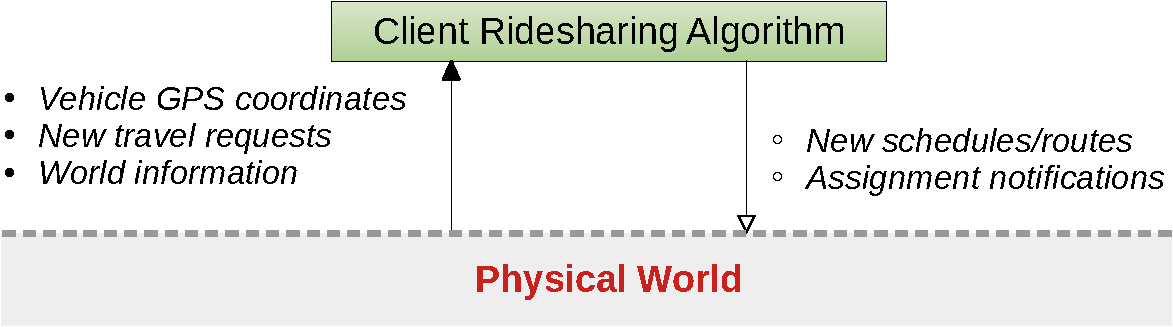
\includegraphics[width=100mm]{fig/physical}
\caption{To evaluate quality, ridesharing algorithms can be tested on physical
vehicles and customers, but this method is expensive, slow to deploy, and out
of reach for most researchers.}
\label{fig:physical}
\end{figure}

Jargo is the name of our environment for evaluating the quality of ridesharing
algorithms (Figure~\ref{fig:architecture}). It captures assignment dependence
by simulating real-time motion of vehicles and capacity, and it simulates
stochastic processes by perturbing route segment durations and locations. To
simulate real-time, it executes a ridesharing algorithm in parallel alongside
new requests so that an algorithm can be running while requests are arriving.
This chapter explains how Jargo's simulation data is organized, beginning with
a description of physical ridesharing (\S\ref{ch:1:sec:ridesharing-systems}),
then the mathematical model to describe physical ridesharing
(\S\ref{ch:1:sec:ridesharing-formulation}), and finally the SQL schema to store
the state data (\S\ref{ch:1:sec:ridesharing-data-model}).

\begin{figure}[h]
\centering
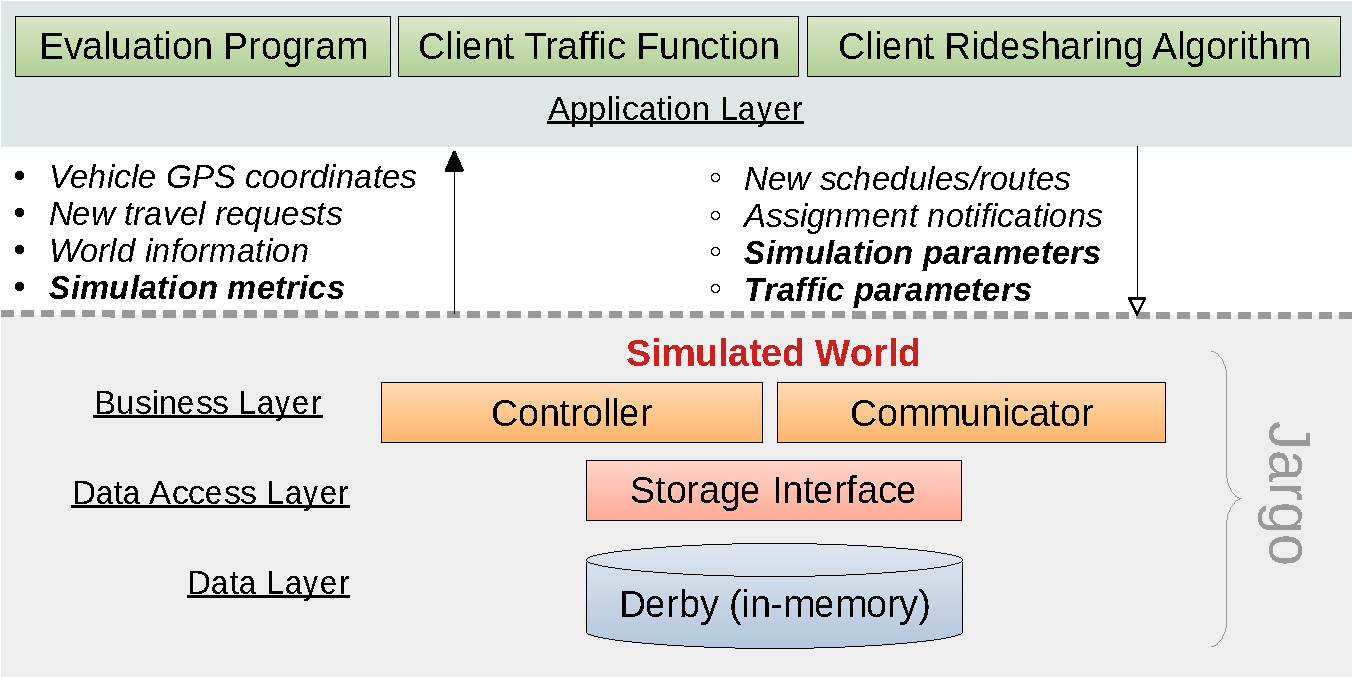
\includegraphics[width=120mm]{fig/architecture}
\caption{Alternatively, ridesharing algorithms can be evaluated on a software
simulator such as Jargo. The architecture and Jargo's ridesharing data model
are designed to protect simulation integrity and to provide analysis
capabilities.}
\label{fig:architecture}
\end{figure}

\section{Ridesharing Systems}
\label{ch:1:sec:ridesharing-systems}
To determine the best way to organize the state data, we first start with
examining real-world ridesharing systems.  Ridesharing involves the
\emph{users} and the \emph{rules} governing their behavior. The users can be
classified into four types, shown in Table~\ref{tab:user-types}.  We use the
term \emph{customer} to refer to both Type 1 and Type 2 users, and the term
\emph{vehicle} to refer to both Type 3 and Type 4 users.  Physical users have
the properties in Table~\ref{tab:user-properties} and obey the rules in
Table~\ref{tab:user-rules}.
\begin{table}[h]
\centering
\small
\caption{Types of ridesharing users.}
\label{tab:user-types}
\begin{tabular}{|l|l|}
\hline
Type   & Description \\
\hline
Type 1 & Single customer traveling alone \\
Type 2 & Group of customers traveling together \\
\hline
Type 3 & Ridesharing vehicle with a predefined final
    destination\footnote{For example a carpooling vehicle.} \\
Type 4 & Taxi-like vehicle continually serving customers without an
    explicit destination of its own\footnote{A Type 4 vehicle could have an
    eventual destination, for example a refueling station; but if the latest
    acceptable arrival time is outside the time span of the ridesharing
    scenario of interest, the destination is not considered. Otherwise, the
    vehicle would be classified as Type 3.}. \\
\hline
\end{tabular}
\caption{Ridesharing user properties.}
\label{tab:user-properties}
\begin{tabular}{|c|p{140mm}|}
\hline
Label & Description \\
\hline
P1 & \hi{Load.} Each user has a non-zero \emph{load}, indicating a
number of needed seats. For Type 1 users the load is 1, indicating they only
need a single seat. For Type 2 users the load exceeds 1. For Type 3 and Type 4
users the load is negative, indicating they have an availability of seats. \\
\hline
P2 & \hi{Origin and Destination.} Each user has an \emph{origin} and a
\emph{destination}, except for Type 4 users that only have an origin.  For Type
1 and Type 2, the origin indicates the initial location of the customer
and the destination indicates the desired final location.  For Type 3, the
origin and destination indicate where the vehicle's ridesharing service begins
and ends.\\
\hline
P3 & \hi{Time Window.} Each user has an \emph{early time} and a
\emph{late time}, together forming the user's \emph{time window}. For a Type 1
or Type 2 customer, the time window gives the desired departure time from the
origin and the desired arrival time at the destination.  For a Type 3 or Type 4
vehicle, the time window gives the time when service begins and the latest time
that service can end. The early time precedes the late time.\\
\hline
\end{tabular}
\caption{Rules bounding user behavior.}
\label{tab:user-rules}
\begin{tabular}{|c|p{140mm}|}
\hline
Label & Description \\
\hline
P4 & \hi{Motion.} Users are bound to a network of roads, for
example the streets of a city. Only vehicles may directly travel along the
roads, whereas customers must be serviced by a vehicle. Both customers and
vehicles may enter the system at any time and anywhere.\\
\hline
P5 & \hi{Pick-ups and Drop-offs.} For a vehicle to service a customer, it
must first travel to the customer's origin to pick up the customer, and then to
the customer's destination to drop off the customer, in that order. The
customer enters the vehicle during the pick-up and exits the vehicle during the
drop-off. These visits must occur within the customer's time window\footnote{We
limit our scope to the typical case where a customer is served by only one
vehicle (no transfers).}.\\
\hline
P6 & \hi{Vehicle Seats.} When a customer enters a vehicle, the customer
occupies a number of seats equal to the customer's load. When it exits the
vehicle, it relinquishes the seats. At no time can the number of occupied seats
exceed the number of available seats in a vehicle.\\
\hline
P7 & \hi{User States.} A customer can be in one of three states at any
time: \emph{waiting} for pick-up; \emph{in-transit} following a pick-up but
before the drop-off; or \emph{arrived} at destination. A vehicle can be either
\emph{in-service} or \emph{out-of-service}.\\
\hline
\end{tabular}
\end{table}

\section{Ridesharing Formulation}
\label{ch:1:sec:ridesharing-formulation}
We can now try to mathematically describe the system.  Users can naturally be
described by a set of values for their P1--P3 properties.  Each vehicle can
also be associated with a sequence of values describing its past and future
motion (P4); a set of values indicating when and where pick-ups and drop-offs
have occurred (P5); and a value to indicate the number of available seats at
any given time (P6). Each customer can be associated with a value indicating
its state (P7). Moreover, the ridesharing setting, namely the road network, can
be described using sets of values indicating coordinates and distances in the
network.

Now that we know what values we have, we can try to organize the data into variables
and constants and write equations to explain the relationships. If we
organize the data into \emph{relations}, we can use selection and projection
when we write the equations. These operations will turn out to be useful for
formalizing certain concepts such as pick-up and drop-off times for a customer
or the cruising and service distance for a vehicle.

\subsection*{Relations}
The following briefly overviews the concept of relations and introduces some
notation.
Relations can be defined in terms of \emph{sequences} and \emph{tuples}.
A sequence is an ordered list of elements.
We will write the integer sequence from $i$ to
$j$ as $i..j$. The sequence
$$(a_i)_{i\in 1..n}=a_1,a_2,...,a_{n-1},a_n$$
will be written $a_1..a_n$ or simply $a$ (without any subscript).
The number of elements in $a$ is called the \emph{length}
of $a$ and is expressed as $|a|$.
A copy $b$ of sequence $a$ but with some elements removed is called
a \emph{subsequence}.
Sequence $b$ is called a \emph{substring} of $a$
only if some $k$ exists such that $$b=a_{1+k}..a_{|b|+k},$$
in other words the elements in $b$ form a contiguous subsequence of $a$.
We call
sequence $a$ a \emph{tuple} if each element of $a$ is labeled. A
labeled element is called a \emph{component}.
A function mapping an element based on its position in the tuple to a label
is called a \emph{labeling scheme}.
Each component also has a \emph{domain} from which the component takes its value,
for example the set of real numbers.
A tuple of length $m$ is called an $m$-tuple. A 2-tuple is called a
\emph{pair}.
A tuple definition will be written as its labels surrounded by parentheses with the
domains given. Label names will be written in \texttt{typewriter} script
to avoid confusion with positional indices.

\begin{example}
\label{ex:tuple}
The sequence $a=a_\texttt{x},a_\texttt{y}$
is a 2-tuple with components named \texttt{x} and \texttt{y}.
The labeling
scheme for $a$ maps $1\rightarrow \texttt{x}$ and $2\rightarrow \texttt{y}$, with the
integers $1$ and $2$ referring to the position of the elements. A possible definition for
$a$ could be $a:=(\texttt{x},\texttt{y}),
a_\texttt{x}\in\mathbb{R}, a_\texttt{y}\in\{\textrm{cat},\textrm{dog}\}.$
\end{example}

A set of unique $m$-tuples with the same labeling scheme is called
an \emph{$m$-ary relation}, or simply relation.
Two operators can be applied onto relations\footnote{Our model is not concerned with joins.}.
The \emph{selection operator} $\sigma_P(R)$ is a function that returns a subset
$R'\subseteq R$ such that predicate $P(R'_i)$ is true for each tuple $R'_i\in R'$.
The \emph{projection} operator $\pi_L(R)$ is a function that returns a copy
$R'$ of $R$ such that each tuple $R'_i\in R'$ is distinct, and only components
with a label in set $L$ are included.

Observe that an $m$-tuple is an $m$-ary relation with one element.
The projection operator thus naturally applies to tuples. For instance, see that for
$R=R_\texttt{x},R_\texttt{y}:=(\texttt{x},\texttt{y}),$
the $\texttt{x}$ component is extracted with
$R_\texttt{x}=\pi_\texttt{x}(R)$
and the $\texttt{y}$ component is extracted with
$R_\texttt{y}=\pi_\texttt{y}(R)$.

\subsection{Setting}
\label{ch:1:sec:setting}
Now we begin to assign variables and constants to the ridesharing
system, starting with the setting.

\hi{Time.} Time is considered to be a positive integer $1\leq t\leq H$.  A
\emph{time horizon} $H$ is introduced to bound the system.

Time will occasionally need to be operated on.  Times cannot be added, and only
a later (greater) time can subtract an earlier (lesser) time.  The difference
is called a \emph{duration}, represented by the symbol $\delta$.  Durations can
add and subtract each other to get new durations, and times can also add and
subtract durations to get new times.

\hi{Road Network.}
The road network is considered to be a directed graph $\mathcal{G}(\mathcal{V},\mathcal{E})$.
Vertices in $\mathcal{V}$ represent points along roads in the network.
A function ${V:\mathcal{V}\rightarrow \mathbb{R}^2}$ maps vertices to
$2$-dimensional latitude and longitude coordinates in the real world.
An inverse function can be used to map-match customers and vehicles to vertices.
Edges in $\mathcal{E}$ represent road segments. The pair $(a,b)\in
\mathcal{V}^2, a\neq b$ exists in $\mathcal{E}$ only if physical traffic flows from
$V(a)$ to $V(b)$, and for all $c\in \mathcal{V}\setminus\{a,b\}$ no traffic flows from
$V(a)$ to $V(c)$ and from $V(c)$ to $V(b)$.
A function ${d:\mathcal{E}\rightarrow\mathbb{R}_{>0}}$ maps edges to positive real weights
corresponding to distance along the edge. See that the
shortest-path distances between the pairs among any three vertices satisfies the
triangle inequality.

\begin{figure}[h]
\centering
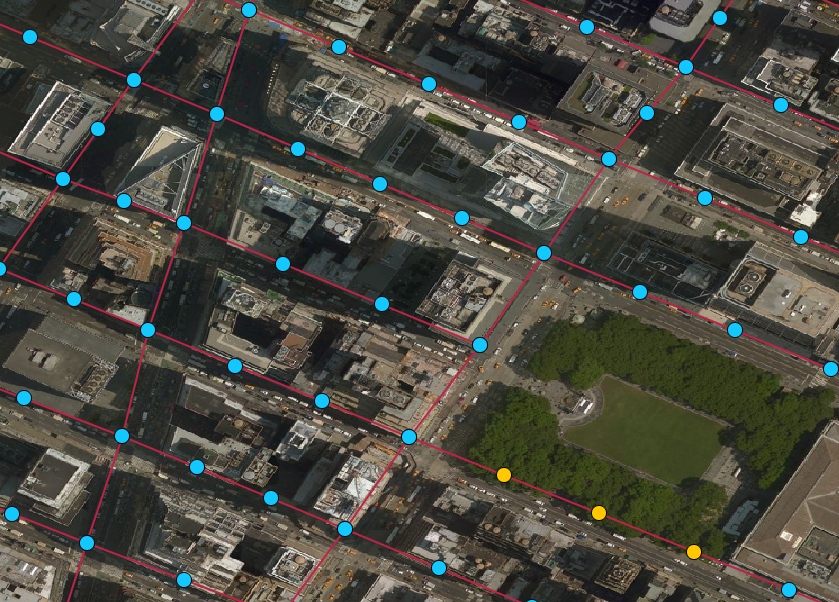
\includegraphics[width=0.8\textwidth]{fig/road}
\caption{Portion of a road network graph showing edges (red lines) and vertices
(blue circles) overlayed on top of Manhattan (QGIS 2.18.16, Bing Aerial).
Vertices do not have to be at an intersection (orange circles, lower right).}
\label{fig:road}
\end{figure}

\hi{Paths.}
A path $p=(p_i)_{i\in 1..n}=p_1..p_n$ is a sequence of $n$ vertices
such that any two adjacent vertices are an edge, or $(p_i,p_{i+1})\in \mathcal{E}$ for
$i\in 1..(n-1)$.
A vertex or edge can appear multiple times in a path.
The \emph{path distance} is
$$\sum_{i=1}^{n-1} d(p_i, p_{i+1}).$$
Path $p$ is a \emph{shortest path} only if it minimizes the distance out of all
possible paths from $p_1$ to $p_n$.
Multiple shortest paths are possible.

\hi{Waypoints.}
Waypoints are used to describe points in time as well as space.
A waypoint is a tuple $(\texttt{t},\texttt{v})$, with the
domain of $\texttt{t}$ as $1..H$ and the domain of $\texttt{v}$ as
$\mathcal{V}$. Waypoints can be labeled in a way that will be
discussed later.

\hi{Routes.}
Routes are formed by a sequence of waypoints. A route
$w=(w_i)_{i\in 1..n}=w_1..w_n=(t_1,v_1)..(t_n,v_n)$
is defined as a sequence of $n$ waypoints such that
$t_1..t_n$ is strictly increasing and $v_1..v_n$ is a path.
%In other words it is a binary relation on time and $\mathcal{V}$.
In the spatial dimension, function
$$D(w)=\sum_{i=1}^{n-1}d(\pi_\texttt{v}(w_i),\pi_\texttt{v}(w_{i+1}))$$
gives the \emph{route distance}, analogous to path distance.
% Abandoned: wordy. Projection $\pi_\texttt{v}(w_i)$ returns the vertex component of waypoint $w_i$.
In the time dimension, function
$$\delta(w)=\pi_\texttt{t}(w_n)-\pi_\texttt{t}(w_1)$$
gives the \emph{route duration}.
%The \emph{distance} of $w$ is $D(\pi_\texttt{v}(w))$.
%The \emph{duration} of $w$ is $t_n$.
Given a time $t$,
\begin{align*}
w_{\leq t}=\textrm{sort}(\sigma_{\texttt{t}\leq t}(w))\quad\textrm{and}\quad
w_{>t}=\textrm{sort}(\sigma_{\texttt{t}>t}(w))
\end{align*}
give the \emph{traveled route} denoted $w_{\leq t}$, and the \emph{remaining
route} denoted $w_{>t}$. As the selection operator imposes no ordering on the resulting
set, a $\textrm{sort}(...)$ function is introduced to
sort a set of waypoints by time in ascending order, returning a sequence.
% From now on, any selection or projection on time is assumed to be sorted
% in this manner.
For two adjacent waypoints $w_i$ and~$w_{i+1}$, function
$$\nu(w_i,w_{i+1})=\frac{d(\pi_\texttt{v}(w_i),\pi_\texttt{v}(w_{i+1}))}
{\pi_\texttt{t}(w_{i+1})-\pi_\texttt{t}(w_i)}$$ gives the
\emph{waypoint rate}, or more intuitively the \emph{speed}.
% The unit of speed depends on the units of $d$ and time and do not have to be
% a physical velocity, such as meters per second.
As $d$ only applies to edges, $\nu$ only applies to adjacent waypoints.
Speeds can be bounded above by a value $\nu^\textrm{max}(v_i,v_{i+1})$ on each edge,
for example to describe road speed limits.
%The speed limit can be different
%on different edges, but to simplify the notation, let $\nu_{max}$ denote the limit for any edge.
%Note that duration $t_n$ and distance $D(\pi_\texttt{v}(w))$ are
%convertible through the speeds along each of the edges.

\subsection{Requests and Servers}
\label{ch:1:sec:requests-and-servers}
Now we define the requests and servers.
The basic entity representing a ridesharing participant is the \emph{user}.  A
user is classified as a \emph{request} if it represents a Type~1 or Type~2
customer, or classified as a \emph{server} if it represents a Type~3 or Type~4
vehicle. As only vehicles can move about (P4), only servers are associated with
routes in order to describe the motions. Later, \emph{schedules} describing
pick-up and drop-off events will be defined on the routes.

\hi{User Relation}
A user $u$ is a 5-tuple defined by
${u:=(\texttt{q},\texttt{e},\texttt{l},\texttt{o},\texttt{d})}$.  The
\texttt{q} component corresponds to the user load; the \texttt{e} and
\texttt{l} components correspond to the user early and late times; the
\texttt{o} and \texttt{d} components correspond to the user origin and
destination.
From P1--P4, the domain of \texttt{q} is the non-zero integers; the domain of \texttt{e} is
$1..(H-1)$ and the domain of \texttt{l} is $(u_\texttt{e}+1)..H$; the domains
of \texttt{o} and \texttt{d} are both $\mathcal{V}$.
For a Type 4 vehicle, the destination can be set to a dummy vertex with edge
weight equal to 0 to every other vertex in the road network.

The set of all users forms the 5-ary relation $\mathcal{U}$, called
the \emph{user relation}.
The set
$\mathcal{U}_\texttt{o}=\pi_\texttt{o}(\mathcal{U})$ contains all origins and
$\mathcal{U}_\texttt{d}=\pi_\texttt{d}(\mathcal{U})$ contains all destinations.
From P1, a user can be classified as either a request or a server based on its load.

From now on as a convenience, the notation $d_u$ will be used to denote the distance of the
shortest path from $u_\texttt{o}$ to $u_\texttt{d}$ on graph $\mathcal{G}$, and
the notation $\delta_u$ will be used to denote the shortest travel duration
along $d_u$ using the speed limits $\nu^\textrm{max}$ along the shortest-path edges.

\hi{Requests.}
A request represents a Type 1 or Type 2 customer.
According to P1,
relation $\mathcal{R}\subseteq\mathcal{U}$,
$$\mathcal{R}=\sigma_{\texttt{q}>0}(\mathcal{U}),$$
% Abandoned: $$\mathcal{R}=\{r\in \mathcal{U}\mid r_\texttt{q}>0\},$$
forms the set of all requests by taking users with positive loads. The set
$\mathcal{R}_\texttt{o}=\pi_\texttt{o}(\mathcal{R})$ is the set of all request origins and
$\mathcal{R}_\texttt{d}=\pi_\texttt{d}(\mathcal{R})$ is the set of all request destinations.
%Abandoned: "corresponding" vertices
%Abandoned: Vertex $v$ is a \emph{pickup} if $v\in \mathcal{R}_o$ and it is a
%\emph{dropoff} if $v\in \mathcal{R}_d$.

\hi{Servers.}
Likewise, a server represents a Type 3 or Type 4 vehicle.
From P1, the relation $\mathcal{S}=\mathcal{U}\setminus\mathcal{R}$, or
$$\mathcal{S}=\sigma_{\texttt{q}<0}(\mathcal{U}),$$
% Abandoned: $$\mathcal{S}=\{s\in \mathcal{U}\mid s_\texttt{q}<0\},$$
forms the set of all servers. The set
$\mathcal{S}_\texttt{o}=\pi_\texttt{o}(\mathcal{S})$ is the set of all server origins and
$\mathcal{S}_\texttt{d}=\pi_\texttt{d}(\mathcal{S})$ is the set of all server destinations.
%Abandoned: The vehicle has a speed $\nu(a,b)$ along edge $(a,b)$. For
%simplicity, denote the speed as $\nu$ for all vehicles and all edges.

\hi{Routes and Schedules}
To encode vehicle motions, each server $s\in\mathcal{S}$ is associated with a
route and a schedule.  A server's route is a representation of the corresponding
vehicle's motion through the road network while a server's schedule
encodes the times and locations of customer pick-ups and drop-offs.
The schedule describes the events along the route and not any new motion,
therefore it is a subsequence of the server's route.

\hi{Server Routes.}
Let $w$ be the route for server $s$. As time
advances, the traveled route $w_{\leq t}$ encodes the server's past
motion while the remaining route $w_{>t}$ encodes the future motion.
From P2 and P3, the route is subject to two rules:
\begin{enumerate}
\item[R1.] The time component of the first waypoint equals the server's early time,
  and the time component of the last waypoint is not greater than the server's late time,
  or $\pi_\texttt{t}(w_1)=s_\texttt{e}$ and $\pi_\texttt{t}(w_{|w|})\leq s_\texttt{l}$;
\item[R2.] The vertex components of the first and last waypoints equal the
  server's origin and destination respectively, or
  $\pi_\texttt{v}(w_1)=s_\texttt{o}$ and $\pi_\texttt{v}(w_{|w|})=s_\texttt{d}$.
\end{enumerate}

\hi{Server Schedules.}
A server's schedule
$$b=(b_j)_{j\in 1..m}=(w_{i_j})_{j\in 1..m}=(t_{i_1},v_{i_1})..(t_{i_m},v_{i_m})$$
is a subsequence of the server's route $w$, with $m\leq |w|$ waypoints.
First:
\begin{enumerate}
\item[R3.] The first and last waypoints $b_1$ and $b_m$ equal the first and last
waypoints of $w$, or ${b_1=w_1}$ and ${b_m=w_{|w|}}$.
\end{enumerate}
This rule will help later when defining departure and arrival times.
Second, from P5:
\begin{enumerate}
\item[R4.] For each waypoint $b_j$ for $j\in 2..(m-1)$, the vertex component is either a
request origin or request destination, or $\pi_\texttt{v}(b_j)\in
\mathcal{R}_\texttt{o}\cup\mathcal{R}_\texttt{d}$.
\end{enumerate}
In other words, each entry or exit must occur at a customer origin or destination.

A schedule formalizes the notion of shared travel with other users, as
multiple entries and exits can overlap within the same server route.
At time $t$, the \emph{traveled schedule} denoted $b_{\leq t}$ encodes the past entries and exits and is given by
$\sigma_{\texttt{t}\leq t}(b)$. Likewise, the \emph{remaining schedule} denoted
$b_{>t}$ encodes the future entries and exits and is given by $\sigma_{\texttt{t}>t}(b)$.

\hi{Schedule Labels.}
Each waypoint in schedule $b$ has a set of labels in order to identify which
customers are entering and exiting the vehicle at the waypoint's time and location.
A labeling scheme can be applied to $b$ to determine each of the labels. The
set of all possible labels depends on the locations of the waypoints. Let
$$\mathcal{R}'=\sigma_{\texttt{o}\in\pi_\texttt{v}(b)\lor \texttt{d}\in\pi_\texttt{v}(b)}(\mathcal{R})$$
%Abandoned: $$\mathcal{R}'=\{r\in \mathcal{R}\mid
%     r_\texttt{o}\in\pi_\texttt{v}(b)\vee r_\texttt{d}\in\pi_\texttt{v}(b)\}$$
give the set of requests whose origin or destination is found
in at least one waypoint in $b$. The labeling scheme
\begin{equation*}
L:b\rightarrow \mathbb{P}(\mathcal{R}'\cup\{s\})
\end{equation*}
maps elements of $b$ to elements of the power set of $\mathcal{R}'\cup\{s\}$.
By using the power set $\mathbb{P}$,
a waypoint can have multiple labels, representing the case where multiple customers
enter or exit the vehicle at the waypoint.
The labeling scheme is subject to the following labeling rules:
\begin{enumerate}
\item[R5.] No waypoint can be labeled with $r\in\mathcal{R}'$ if a schedule for another server
already contains waypoints labeled with $r$;
\item[R6.] A waypoint $b_j\in b$ can be labeled with $r$ only if
$\pi_\texttt{v}(b_j)=r_\texttt{o}$ or $\pi_\texttt{v}(b_j)=r_\texttt{d}$;
\item[R7.] If $b_j$ is to be labeled with $r$ and $\pi_\texttt{v}(b_j)=r_\texttt{o}$, then
a second waypoint $b_{j'}$ such that $j'>j$ and
$\pi_\texttt{v}(b_{j'})=r_\texttt{d}$ must also be labeled with $r$;
\item[R8.] The time components of $b_j$ and $b_{j'}$ must be within request $r$'s time window,
formally $r_\texttt{e}\leq \pi_\texttt{t}(b_j)$ and $\pi_\texttt{t}(b_{j'})\leq r_\texttt{l}$;
\item[R9.] The number of waypoints labeled with $r$ must be exactly 0 or 2;
\item[R10.] The first and last waypoints must contain the schedule's server $s$
in their labels, and no other waypoint can be labeled with $s$.
\end{enumerate}
Rules R5--R9 express P5.  Rule R10 can be interpreted to mean that a vehicle
must ``serve itself'' at its own origin and destination.  This last rule
helps to define later concepts.

\hi{Server Relation}
By combining the routes, schedules, and labels into
a set of $(\texttt{s},\texttt{t},\texttt{v},\texttt{L})$ tuples, a
4-ary relation $\mathcal{X}$ can be formed. This relation is called the
\emph{server relation} and as will be shown soon, it is the basis for computing many common ridesharing metrics.
Each tuple associates the waypoint in the \texttt{t} and \texttt{v} components with the server
in the \texttt{s} component, along with the labels in the \texttt{L} component.
% The domain of $\texttt{s}$ is $\mathcal{S}$; the domain of $\texttt{t}$ is
% $1..H$; the domain of $\texttt{v}$ is $\mathcal{V}$; the domain of $\texttt{L}$
% is the power set $\mathbb{P}(\mathcal{U})$.

A server's route can be recovered by extracting \texttt{t} and \texttt{v}
components and sorting by time, or formally for a given server $s$, its route
is given by
$$W(\mathcal{X},s)=\textrm{sort}(\pi_{\texttt{t},\texttt{v}}(\sigma_{\texttt{s}=s}(\mathcal{X}))).$$
Similarly, a server's schedule can be recovered by
extracting only those waypoints that are labeled, formally
$$B(\mathcal{X},s)=\textrm{sort}(\pi_{\texttt{t},\texttt{v}}(\sigma_{\texttt{s}=s\land |\texttt{L}|>0}(\mathcal{X}))).$$

The server relation can be used to define the remaining physical concepts, P6 and P7.

\hi{Request Status.}
Given a request $r$, the function
\begin{equation}
\label{eq:status}
\textrm{status}(\mathcal{X},r,t)=|\sigma_{\texttt{t}\leq t\land
r\in\texttt{L}}(\mathcal{X})|
\end{equation}
gives the count of the tuples labeled with $r$
before or on a given time. From the labeling rules, the count can be only 0, 1,
or 2. See that these counts correspond to request waiting, in-transit, and arrived states
from P7, respectively.

Given a server $s$, knowing the in-transit requests for $s$ can be useful for
pricing and other rider-related
metrics. %~\cite{DBLP:conf/sigmod/ChengX017,DBLP:conf/dexa/ShiLZG17,DBLP:conf/ijcai/SantosX13}.
These requests can be easily found by
$$\mathcal{Q}(\mathcal{X},s,t)=\{r\in\mathcal{R}\mid\textrm{status}(\mathcal{X},r,t)=1
\land\pi_\texttt{s}(\sigma_{r\in\texttt{L}}(\mathcal{X}))=s\}.$$

\hi{Load Burden.}
The \emph{load burden} on $s$ can be computed using the in-transit requests by
\begin{equation}
\label{eq:load}
Q(\mathcal{X},s,t)=\sum_{r\in\mathcal{Q}(\mathcal{X},s,t)}r_\texttt{q}.
\end{equation}
From P6, server routes are subject to the additional rule:
\begin{enumerate}
\item[R11.] $Q(\mathcal{X},s,t)\leq -s_\texttt{q}$ must be true for all $s$ and $t$.
\end{enumerate}

\subsection{Ridesharing Metrics}
\label{ch:1:sec:ridesharing-metrics}
As a benefit from using relations, a variety of metrics can now be measured by
simple operations on $\mathcal{U}$ and $\mathcal{X}$.  The following lists
common metrics found in existing ridesharing studies, but others may be possible.

\hi{Assignments.}
Server $s$ is said to be \emph{assigned to} request $r$ at time $t$ only if
$\textrm{status}(\mathcal{X},r,t)=2$. That is, the request's status is arrived at time $t$.
The set of $(s,r)$ pairs
where this property is true is called the set of \emph{assignments}, formally
\begin{equation}
\label{eq:assignments}
\textit{assignments }A(\mathcal{X},t)=
\{(s,r)\in\mathcal{S}\times \mathcal{R} \mid \textrm{status}(\mathcal{X},r,t)=2\}.
\end{equation}
Using the assignments,
\begin{align}
\label{eq:assigned-requests}
\textit{assigned requests }R^\textrm{ok}(\mathcal{X},t)&=\pi_\texttt{r}(A(\mathcal{X},t))\textrm{, and}\\
\label{eq:unassigned-requests}
\textit{unassigned requests }R^\textrm{ko}(\mathcal{X},t)&=\mathcal{R}\setminus\mathcal{R}^\textrm{ok}(\mathcal{X},t).
\end{align}
The server assigned to $r$ can be obtained with
\begin{equation}
S(\mathcal{X},r,t)=\{s\in\mathcal{S}\mid\textrm{status}(\mathcal{X},r,t)=2\},
\end{equation}
guaranteed to return only one server due to R5.
Likewise, the set of requests assigned to $s$ can be obtained with
\begin{equation}
\label{eq:R(X,s,t)}
R(\mathcal{X},s,t)=\{r\in\mathcal{R}\mid\textrm{status}(\mathcal{X},r,t)=2\}.
\end{equation}

\hi{Service rate.}
The \emph{service rate} is the number of assigned requests over the number of all requests, or
\begin{equation}
\label{eq:service-rate}
\textit{service rate }\mu(\mathcal{X},t)=\frac{|R^\textrm{ok}(\mathcal{X},t)|}{|\mathcal{R}|}.
\end{equation}

\hi{Distances.}
The \emph{base distance} is the sum of the shortest-path distances for all users, or
\begin{equation}
\label{eq:base-distance}
\textit{base distance }D^\textrm{base}(\mathcal{U})=\sum_{u\in U}d_u.
\end{equation}
The \emph{travel distance} for one server $s$ is the distance of its route,
$D(W(\mathcal{X},s))$,
and the \emph{travel duration} can be found with
$\delta(W(\mathcal{X},s))$.

For a server with route $w$, travel distance $D(w)$ can be partitioned into
\emph{cruising distance} $D_0(w)$ and
\emph{service distance} $D_1(w)$.
The cruising distance sums the distance along portions where the load burden is zero.
The service distance sums the distance along portions of $w$ where the
load burden is non-zero.
Formally, partition $w$ into a set of substrings $\Omega(w)$ such that each waypoint
in $w$ is a member of exactly one substring and that for all substrings $\omega\in \Omega$,
\begin{align}
\label{eq:slack}\textrm{either }Q(\mathcal{X},s,t)&=0\textrm{ is true for all }t\in \pi_\texttt{t}(\omega),\\
\label{eq:block}\textrm{or }Q(\mathcal{X},s,t)&>0\textrm{ is true for all }t\in \pi_\texttt{t}(\omega).
\end{align}
%Observe that Eqs.~\ref{eq:slack}~and~\ref{eq:block}
%formalize concepts similar to the intuitive
%\emph{slack periods} and \emph{schedule blocks} in~\cite{jaw:1986}.
The equations can be used to partition $\Omega(w)$ into two subsets,
\begin{align*}
\Omega_0(w)&=\{\omega\in \Omega(w)\mid \omega\textrm{ satisfies Eq.~\ref{eq:slack}}\}\textrm{ and }\\
\Omega_1(w)&=\{\omega\in \Omega(w)\mid \omega\textrm{ satisfies Eq.~\ref{eq:block}}\}.
\end{align*}
The distances of each of the substrings in each subset can be summed
to get
$$D_0(w)=\sum_{\omega\in \Omega_0(w)} D(\omega)\quad\textrm{and}\quad
  D_1(w)=\sum_{\omega\in \Omega_1(w)} D(\omega).$$
These distances are written as
\begin{align}
\label{eq:cruising-distance}
\textit{cruising distance }D^\textrm{cruise} (\mathcal{X},s)&=D_0(W(\mathcal{X},s)),\textrm{ and}\\
\label{eq:service-distance}
\textit{service distance } D^\textrm{service}(\mathcal{X},s)&=D_1(W(\mathcal{X},s)).
\end{align}

\hi{Detours and Delays.}
In physical terms, the \emph{detour route} for a customer is the portion of a vehicle's
route between when it visits the customer's origin and destination. Formally, let
%\item $d_r$ be the distance of the shortest path from $r_\texttt{o}$ to $r_\texttt{d}$;
$w=W(\mathcal{X},S(\mathcal{X},r,H))$ be the route of the server assigned to $r$.
The detour route $\Delta W(\mathcal{X},r)$ is an $m$-length substring of $w$ given by
$\Delta W(\mathcal{X},r)=w_{1+k}..w_{m+k}$ such that for some $k$,
\begin{itemize}
\item $\Delta W(\mathcal{X},r)$ begins at $r_\texttt{o}$, or $\pi_\texttt{v}(w_{1+k})=r_\texttt{o}$,
\item $\Delta W(\mathcal{X},r)$ ends at $r_\texttt{d}$, or $\pi_\texttt{v}(w_{m+k})=r_\texttt{d}$, and
\item the first and last waypoints of $\Delta W(\mathcal{X},r)$ are labeled with $r$, or $r\in\pi_\texttt{L}(w_{1+k})\cap\pi_\texttt{L}(w_{m+k})$.
\end{itemize}
Observe that due to the labeling rules, only one value of $k$ can satisfy these
conditions. The first and last waypoints $w_{1+k}$ and $w_{m+k}$ can be found by
the equations on users,
\begin{align}
\label{eq:pickup}
\textrm{pickup}(\mathcal{X},u)&=\pi_{\texttt{t},\texttt{v}}(\sigma_{\texttt{v}=u_\texttt{o}\land u\in\texttt{L}}(\mathcal{X}))\textrm{, and}\\
\label{eq:dropoff}
\textrm{dropoff}(\mathcal{X},u)&=\pi_{\texttt{t},\texttt{v}}(\sigma_{\texttt{v}=u_\texttt{d}\land u\in\texttt{L}}(\mathcal{X})),
\end{align}
by substituting $r$ for $u$.
Note that if a server is substituted for $u$, these equations give the start and
end waypoints of the server's route due to R3 and R10.
These two equations can also be used to give two times for
any user,
\begin{align}
\label{eq:departure-time}
\textit{departure time }t^\textrm{depart}(\mathcal{X},u)&=\pi_\texttt{t}(\textrm{pickup}(\mathcal{X},u))\textrm{, and}\\
\label{eq:arrival-time}
\textit{arrival time }t^\textrm{arrive}(\mathcal{X},u)&=\pi_\texttt{t}(\textrm{dropoff}(\mathcal{X},u)).
\end{align}
In the real world, the time until a vehicle picks up a customer can be of interest.
This \emph{pick-up delay} can be found with
\begin{equation}
\label{eq:pick-up delay}
\textit{pick-up delay }\delta^\textrm{pickup}(\mathcal{X},r)=\pi_\texttt{t}(\textrm{pickup}(\mathcal{X},r))-r_\texttt{e}.
\end{equation}

The detour route $\Delta W(\mathcal{X},r)$ can only apply to assigned requests. If
a detour route exists, then
the \emph{transit} distance and duration are
\begin{align}
\label{eq:transit-distance}
\textit{transit distance }D^\textrm{transit}(\mathcal{X},r)&=D(\Delta W(\mathcal{X},r))\textrm{, and}\\
\label{eq:transit-duration}
\textit{transit duration }\delta^\textrm{transit}(\mathcal{X},r)&=\delta(\Delta W(\mathcal{X},r)).
\end{align}
Similarly, the \emph{detour} distance and duration are
\begin{align}
\label{eq:detour-distance}
\textit{detour distance }D^\textrm{detour}(\mathcal{X},r)&=D^\textrm{transit}(\mathcal{X},r)-d_r\textrm{, and}\\
\label{eq:detour-duration}
\textit{detour duration }\delta^\textrm{detour}(\mathcal{X},r)&=\delta^\textrm{transit}(\mathcal{X},r)-\delta_r.
\end{align}
Finally, the \emph{travel duration} is the sum of the pick-up and transit durations,
\begin{equation}
\label{eq:travel-duration}
\textit{travel duration }\delta^\textrm{travel}(\mathcal{X},r)=\delta^\textrm{pickup}(\mathcal{X},r)+\delta^\textrm{transit}(\mathcal{X},r)
=\pi_\texttt{t}(\textrm{dropoff}(\mathcal{X},r))-r_\texttt{e}.
\end{equation}

\hi{Utilization.}
The percentage of servers that are assigned to at least one request is given by
\begin{equation}
\label{eq:server-utilization}
\textit{server utilization }\rho^\textrm{server}(\mathcal{X})=\frac{|\pi_\texttt{s}(\mathcal{A}(\mathcal{X}))|}{|\mathcal{S}|}.
\end{equation}
The distance utilization is
\begin{equation}
\label{eq:distance-utilization}
\textit{distance utilization }\rho^\textrm{distance}(\mathcal{X})=
\frac{\sum_{s\in\mathcal{S}}D^\textrm{service}(\mathcal{X},s)}
{\sum_{s\in\mathcal{S}}D(\mathcal{X},s)}.
\end{equation}

\section{Ridesharing Data Model}
\label{ch:1:sec:ridesharing-data-model}
The simple constraints allowed by the SQL standard\footnote{ISO/IEC 9075}
(\texttt{CHECK}, \texttt{UNIQUE}, \texttt{NOT NULL}, \texttt{FOREIGN KEY}) are
unable to express the complex ridesharing properties
(\S\ref{ch:1:sec:ridesharing-systems}, P1--P7) and rules
(\S\ref{ch:1:sec:ridesharing-formulation}, R1--R11), and consequently a direct
``translation'' of the ridesharing relations into SQL is not possible without
either making code extensions to SQL or reorganizing the relational ridesharing
model.

The following schema can be implemented entirely in standard SQL without any
code extensions while staying faithful to the model.  In this schema,
\textit{tables} capture the descriptive elements of the model and
\textit{views} express the analytical measures.  Tables are further organized
into \emph{property}, \emph{solution}, and \emph{constraint} tables.  Property
tables store the road network $\mathcal{G}$ (\S\ref{ch:1:sec:setting}) and the user
relation $\mathcal{U}$ (\S\ref{ch:1:sec:requests-and-servers}).  Solution tables
store the server relation $\mathcal{X}$ (\S\ref{ch:1:sec:requests-and-servers}).
Constraint tables store copies of data from other tables for validation
purposes.  The views are mostly defined on the constraint tables.

Diagrams of the SQL tables are included in this section. In the diagrams,
primary keys are indicated in italics. Elsewhere, column names are
distinguished by \textsf{sans serif} script.  Parentheses are used to logically
group together columns.  A parent table next to a group of columns indicates
foreign key. In SQL, foreign keys must reference their values from the primary
key of the parent table. Many of the table diagrams contain duplicate columns
(for example, \textsf{sid} shows up three times in Table W).  These duplicates
are included for illustrating the foreign key relationships, but in practice
the duplicates are implemented as single columns participating in multiple
foreign keys.

\subsection{Table V and E (Road Network Tables)}
Each vertex $v\in\mathcal{V}$ is stored in Table V along with its coordinates
$V(v)$ while each edge $(a,b)\in\mathcal{E}$ is stored in Table E along with
its weight $d(a,b)$ and speed limit $\nu^\textrm{max}(a,b)$.  Table V thus has
three columns, storing $v$ in primary key column \textsf{v} ({\tt{}P1}) and its
coordinates in column \textsf{lng} and \textsf{lat}.  Likewise, Table E has
four columns, storing $a$ and $b$ in column \textsf{v1} and \textsf{v2},
$d(a,b)$ in column \textsf{dd}, and $\nu^\textrm{max}(a,b)$ in column
\textsf{nu}.  The four columns together form the primary key ({\tt{}P2}) in order
to be referenced by later tables.  Foreign keys on \textsf{v1} ({\tt{}F1}) and
\textsf{v2} ({\tt{}F2}) referencing Table V validate that $a$ and $b$ are actual
vertices.
\begin{table}[h]
\centering
\small
\begin{tabular}{|c|l|}
\hline
\rowcolor{TableTitle}
\multicolumn{2}{|c|}{Table V (Vertices)}\\
\hline
\rowcolor{TableHeader}
Column & Description\\
\hline
\textit{v} & Vertex $v\in\mathcal{V}$\\
\hline
lng & \multirow{2}{*}{Vertex coordinate $V(v)$}\\
lat & \\
\hline
\end{tabular}
\begin{tabular}{|c|c|l|}
\hline
\rowcolor{TableTitle}
\multicolumn{3}{|c|}{Table E (Edges)}\\
\hline
\rowcolor{TableHeader}
Column & Parent & Description\\
\hline
\textit{v1} & Table V & \multirow{2}{*}{Edge $(a, b)\in\mathcal{E}$} \\
\cline{2-2}
\textit{v2} & Table V & \\
\hline
\textit{dd} & & Weight $d(a,b)$\\
\hline
\textit{nu} & & Max. speed $\nu^\textrm{max}(a,b)$\\
\hline
\end{tabular}
\end{table}
\nwenddocs{}\nwbegincode{1}\sublabel{NW3jn8Pl-RzwV3-1}\nwmargintag{{\nwtagstyle{}\subpageref{NW3jn8Pl-RzwV3-1}}}\moddef{Create Table V statement~{\nwtagstyle{}\subpageref{NW3jn8Pl-RzwV3-1}}}\endmoddef\nwused{\\{NWgUSr6-RmKLy-1}}
"CREATE TABLE V ("
  + "v   int  CONSTRAINT P1 PRIMARY KEY,"
  + "lng int  CONSTRAINT C1 NOT NULL,"
  + "lat int  CONSTRAINT C2 NOT NULL,"
  + "CONSTRAINT C3 CHECK (lng BETWEEN -1800000000 AND 1800000000),"
  + "CONSTRAINT C4 CHECK (lat BETWEEN  -900000000 AND  900000000)"
  + ")"
\nwendcode{}\nwbegindocs{2}We consider vertex 0 to be a dummy vertex where any edged formed by 0 has no
weight. To implement the dummy vertex, we add a constraint ({\tt{}C11}) that
\textsf{dd} must be 0 if either \textsf{v1} or \textsf{v2} is 0.
\nwenddocs{}\nwbegincode{3}\sublabel{NW3jn8Pl-2WHSWQ-1}\nwmargintag{{\nwtagstyle{}\subpageref{NW3jn8Pl-2WHSWQ-1}}}\moddef{Create Table E statement~{\nwtagstyle{}\subpageref{NW3jn8Pl-2WHSWQ-1}}}\endmoddef\nwused{\\{NWgUSr6-RmKLy-1}}
"CREATE TABLE E ("
  + "v1  int  CONSTRAINT C5 NOT NULL,"
  + "v2  int  CONSTRAINT C6 NOT NULL,"
  + "dd  int  CONSTRAINT C7 NOT NULL,"
  + "nu  int  CONSTRAINT C8 NOT NULL,"
  + "CONSTRAINT F1 FOREIGN KEY (v1) REFERENCES V (v),"
  + "CONSTRAINT F2 FOREIGN KEY (v2) REFERENCES V (v),"
  + "CONSTRAINT P2 PRIMARY KEY (v1, v2, dd, nu),"
  + "CONSTRAINT C9 CHECK (nu >= 0),"
  + "CONSTRAINT C10 CHECK (v1 <> v2),"
  + "CONSTRAINT C11 CHECK ("
  + "  CASE WHEN v1 = 0 OR v2 = 0"
  + "    THEN dd = 0"
  + "    ELSE dd > 0"
  + "  END"
  + ")"
  + ")"
\nwendcode{}\nwbegindocs{4}\nwdocspar

\subsection{Table UQ, UE, UL, UO, UD, and UB (User Tables)}
To allow other tables to reference specific user components, the user relation
is partitioned into five 2-column tables, UQ, UE, UL, UO, and UD, by taking
projections on the respective \texttt{q}, \texttt{e}, \texttt{l}, \texttt{o},
and \texttt{d} components. Each row is a key-value pair, storing a unique
\textsf{uid} for user identification as the key alongside the component value,
and each row is also its own primary key.  A sixth table UB is introduced to
store base costs for computing $D^\textrm{base}$ and $\rho^\textrm{distance}$
(\S\ref{ch:1:sec:ridesharing-metrics}).  Table UO and UD can be referenced to Table
V to validate against property P2 and rule P4.
\begin{table}[h]
\centering
\small
\begin{tabular}{|c|c|l|}
\hline
\rowcolor{TableTitle}
\multicolumn{3}{|c|}{User Tables}\\
\hline
\rowcolor{TableHeader}
Table & Columns & Description \\
\hline
UQ & \textit{uid}, \textit{val} & User load $u_\texttt{q}$ \\
UE & \textit{uid}, \textit{val} & User early time $u_\texttt{e}$ \\
UL & \textit{uid}, \textit{val} & User late time $u_\texttt{l}$ \\
UO & \textit{uid}, \textit{val} & User origin $u_\texttt{o}$ \\
UD & \textit{uid}, \textit{val} & User destination $u_\texttt{d}$ \\
UB & \textit{uid}, \textit{val} & User base cost $d_u$ \\
\hline
\end{tabular}
\end{table}
\nwenddocs{}\nwbegincode{5}\sublabel{NW3jn8Pl-llmAG-1}\nwmargintag{{\nwtagstyle{}\subpageref{NW3jn8Pl-llmAG-1}}}\moddef{Create Table UQ statement~{\nwtagstyle{}\subpageref{NW3jn8Pl-llmAG-1}}}\endmoddef\nwused{\\{NWgUSr6-RmKLy-1}}
"CREATE TABLE UQ ("
  + "uid int  CONSTRAINT C12 NOT NULL,"
  + "uq  int  CONSTRAINT C13 NOT NULL,"
  + "CONSTRAINT C14 UNIQUE (uid),"
  + "CONSTRAINT C15 CHECK (uq != 0),"
  + "CONSTRAINT P3 PRIMARY KEY (uid, uq)"
  + ")"
\nwendcode{}\nwbegindocs{6}\nwdocspar
\nwenddocs{}\nwbegincode{7}\sublabel{NW3jn8Pl-sBCgz-1}\nwmargintag{{\nwtagstyle{}\subpageref{NW3jn8Pl-sBCgz-1}}}\moddef{Create Table UE statement~{\nwtagstyle{}\subpageref{NW3jn8Pl-sBCgz-1}}}\endmoddef\nwused{\\{NWgUSr6-RmKLy-1}}
"CREATE TABLE UE ("
  + "uid int  CONSTRAINT C16 NOT NULL,"
  + "ue  int  CONSTRAINT C17 NOT NULL,"
  + "CONSTRAINT C18 CHECK (ue BETWEEN 0 AND 86400000),"
  + "CONSTRAINT C19 UNIQUE (uid),"
  + "CONSTRAINT P4 PRIMARY KEY (uid, ue)"
  + ")"
\nwendcode{}\nwbegindocs{8}\nwdocspar
\nwenddocs{}\nwbegincode{9}\sublabel{NW3jn8Pl-3Q8NSk-1}\nwmargintag{{\nwtagstyle{}\subpageref{NW3jn8Pl-3Q8NSk-1}}}\moddef{Create Table UL statement~{\nwtagstyle{}\subpageref{NW3jn8Pl-3Q8NSk-1}}}\endmoddef\nwused{\\{NWgUSr6-RmKLy-1}}
"CREATE TABLE UL ("
  + "uid int  CONSTRAINT C20 NOT NULL,"
  + "ul  int  CONSTRAINT C21 NOT NULL,"
  + "CONSTRAINT C22 UNIQUE (uid),"
  + "CONSTRAINT C23 CHECK (ul BETWEEN 0 AND 86400000),"
  + "CONSTRAINT P5 PRIMARY KEY (uid, ul)"
  + ")"
\nwendcode{}\nwbegindocs{10}\nwdocspar
\nwenddocs{}\nwbegincode{11}\sublabel{NW3jn8Pl-qCW00-1}\nwmargintag{{\nwtagstyle{}\subpageref{NW3jn8Pl-qCW00-1}}}\moddef{Create Table UO statement~{\nwtagstyle{}\subpageref{NW3jn8Pl-qCW00-1}}}\endmoddef\nwused{\\{NWgUSr6-RmKLy-1}}
"CREATE TABLE UO ("
  + "uid int  CONSTRAINT C24 NOT NULL,"
  + "uo  int  CONSTRAINT C25 NOT NULL,"
  + "CONSTRAINT F3 FOREIGN KEY (uo) REFERENCES V (v),"
  + "CONSTRAINT C26 UNIQUE (uid),"
  + "CONSTRAINT P6 PRIMARY KEY (uid, uo)"
  + ")"
\nwendcode{}\nwbegindocs{12}\nwdocspar
\nwenddocs{}\nwbegincode{13}\sublabel{NW3jn8Pl-1OVMyH-1}\nwmargintag{{\nwtagstyle{}\subpageref{NW3jn8Pl-1OVMyH-1}}}\moddef{Create Table UD statement~{\nwtagstyle{}\subpageref{NW3jn8Pl-1OVMyH-1}}}\endmoddef\nwused{\\{NWgUSr6-RmKLy-1}}
"CREATE TABLE UD ("
  + "uid int  CONSTRAINT C27 NOT NULL,"
  + "ud  int  CONSTRAINT C28 NOT NULL,"
  + "CONSTRAINT F4 FOREIGN KEY (ud) REFERENCES V (v),"
  + "CONSTRAINT C29 UNIQUE (uid),"
  + "CONSTRAINT P7 PRIMARY KEY (uid, ud)"
  + ")"
\nwendcode{}\nwbegindocs{14}\nwdocspar
\nwenddocs{}\nwbegincode{15}\sublabel{NW3jn8Pl-3QSM5L-1}\nwmargintag{{\nwtagstyle{}\subpageref{NW3jn8Pl-3QSM5L-1}}}\moddef{Create Table UB statement~{\nwtagstyle{}\subpageref{NW3jn8Pl-3QSM5L-1}}}\endmoddef\nwused{\\{NWgUSr6-RmKLy-1}}
"CREATE TABLE UB ("
  + "uid int  CONSTRAINT C30 NOT NULL,"
  + "ub  int  CONSTRAINT C31 NOT NULL,"
  + "CONSTRAINT C32 CHECK (ub >= 0),"
  + "CONSTRAINT C33 UNIQUE (uid),"
  + "CONSTRAINT P8 PRIMARY KEY (uid, ub)"
  + ")"
\nwendcode{}\nwbegindocs{16}\nwdocspar

\subsection{Table W (Routes Table)}
Table W has eight columns, \textsf{sid}, \textsf{se}, \textsf{t1}, \textsf{v1},
\textsf{t2}, \textsf{v2}, \textsf{dd}, and \textsf{nu}.  The \texttt{s},
\texttt{t}, and \texttt{v} components of $\mathcal{X}$ are stored in the
(\textsf{sid}, \textsf{t2}, \textsf{v2}) columns.  By definition, the sequence
of vertices in a route must form a path and the speed of adjacent waypoints
cannot exceed the limit $\nu^\textrm{max}$.  To enforce these rules, the
\emph{predecessor} waypoint is stored in the (\textsf{sid}, \textsf{t1},
\textsf{v1}) columns.  The (\textsf{v1}, \textsf{v2}) columns can thus identify
an edge. Columns \textsf{dd} and \textsf{nu} are added to store the weight and
speed limit on the edge, and (\textsf{v1}, \textsf{v2}, \textsf{dd},
\textsf{nu}) is referenced by foreign key to Table E ({\tt{}F19}) to validate the
values. A row-level \texttt{CHECK} constraint ({\tt{}C56}) validates that the
speed $\textsf{dd}/(\textsf{t2}-\textsf{t1})$ is not greater than the maximum
free-flow speed, \textsf{nu}.
\begin{table}[h]
\centering
\small
\begin{tabular}{|c|c|l|}
\hline
\rowcolor{TableTitle}
\multicolumn{3}{|c|}{Table W (Routes)} \\
\hline
\rowcolor{TableHeader}
Col. & Parent & Description \\
\hline
\textit{sid} & Table S & Identification for server $s\in\mathcal{S}$ \\
\hline
sid & \multirow{2}{*}{Table UE} & \multirow{2}{*}{Server early time $s_\texttt{e}$} \\
se & & \\
\hline
sid & \multirow{3}{*}{Table W} & \multirow{3}{*}{Predecessor waypoint $w_{i-1}$} \\
t1 & & \\
v1 & & \\
\hline
\textit{t2} & & \multirow{2}{*}{Waypoint $w_i$} \\
\textit{v2} & & \\
\hline
v1 & \multirow{4}{*}{Table E} & \multirow{4}{*}{Properties of edge $(\pi_\texttt{v}(w_{i-1}),\pi_\texttt{v}(w_i))$} \\
v2 & & \\
dd & & \\
nu & & \\
\hline
\end{tabular}
\end{table}
The below items are easily implemented in SQL and establish that each
(\textsf{sid}, \textsf{t1}, \textsf{v1}) is indeed the predecessor to
(\textsf{sid}, \textsf{t2}, \textsf{v2}) in the same row:
\begin{enumerate}
\item The predecessor (\textsf{sid}, \textsf{t1}, \textsf{v1}) must reference
an existing waypoint (\textsf{sid}, \textsf{t2}, \textsf{v2}) from the table
({\tt{}F20});
\item Out of all rows, (\textsf{sid}, \textsf{t1}) must be unique and
(\textsf{sid}, \textsf{t2}) must be unique ({\tt{}C54}, {\tt{}C55});
\item Column \textsf{t2} and \textsf{v2} cannot be null ({\tt{}C52}, {\tt{}C53});
\item Unless \textsf{t2} is equal to the server's early time, \textsf{t1}
cannot be null and it must be less than \textsf{t2}, otherwise \textsf{t1},
\textsf{v1}, \textsf{dd}, and \textsf{nu} must all be null ({\tt{}C56}).
\end{enumerate}
The (\textsf{sid}, \textsf{t2}, \textsf{v2}) columns are the primary key
({\tt{}P11}) in order to allow the self-referencing foreign key in the first item.
The last item handles the case where the first waypoint in a server's route has
no predecessor. Only in this case are \textsf{t1}, \textsf{v1}, \textsf{dd},
and \textsf{nu} are allowed to be null.  From rule R1, the first waypoint is
detected by checking if \textsf{t2} is equal to the server's early time, stored
in column \textsf{se}. The (\textsf{sid}, \textsf{se}) columns are referenced
to UE to validate the early time ({\tt{}F18}).
\nwenddocs{}\nwbegincode{17}\sublabel{NW3jn8Pl-2FnbXJ-1}\nwmargintag{{\nwtagstyle{}\subpageref{NW3jn8Pl-2FnbXJ-1}}}\moddef{Create Table W statement~{\nwtagstyle{}\subpageref{NW3jn8Pl-2FnbXJ-1}}}\endmoddef\nwused{\\{NWgUSr6-RmKLy-1}}
"CREATE TABLE W ("
  + "sid int  CONSTRAINT C50 NOT NULL,"
  + "se  int  CONSTRAINT C51 NOT NULL,"
  + "t1  int  ,"
  + "v1  int  ,"
  + "t2  int  CONSTRAINT C52 NOT NULL,"
  + "v2  int  CONSTRAINT C53 NOT NULL,"
  + "dd  int ,"
  + "nu  int ,"
  + "CONSTRAINT P11 PRIMARY KEY (sid, t2, v2),"
  + "CONSTRAINT F17 FOREIGN KEY (sid) REFERENCES S,"
  + "CONSTRAINT F18 FOREIGN KEY (sid, se) REFERENCES UE (uid, ue),"
  + "CONSTRAINT F19 FOREIGN KEY (v1, v2, dd, nu) REFERENCES E INITIALLY DEFERRED,"
  + "CONSTRAINT F20 FOREIGN KEY (sid, t1, v1) REFERENCES W (sid, t2, v2) INITIALLY DEFERRED,"
  + "CONSTRAINT C54 UNIQUE (sid, t1),"
  + "CONSTRAINT C55 UNIQUE (sid, t2),"
  + "CONSTRAINT C56 CHECK ("
  + "  CASE WHEN t1 IS NULL"
  + "    THEN t2 = se AND v1 IS NULL AND dd IS NULL AND nu IS NULL"
  + "    ELSE dd/(t2-t1) <= nu AND t1 < t2"
  + "  END"
  + ") INITIALLY DEFERRED"
  + ")"
\nwendcode{}\nwbegindocs{18}\nwdocspar

\subsection{Table PD (Labels Table)}
Table PD (for ``pick-ups and drop-offs'') contains four columns, \textsf{sid},
\textsf{t2}, \textsf{v2}, and \textsf{rid}.  The (\textsf{sid}, \textsf{t2},
\textsf{v2}) columns reference Table W ({\tt{}F23}), and the \textsf{rid} column
indicates the label on that waypoint.  Each row is its own primary key
({\tt{}P12}) in order to be referenced by the CPD constraint table.  A waypoint
can have multiple labels simply by listing the waypoint multiple times with
different values of \textsf{rid}.
\begin{table}[h]
\centering
\small
\begin{tabular}{|c|c|l|}
\hline
\rowcolor{TableTitle}
\multicolumn{3}{|c|}{Table PD (Pick-up and Drop-off Labels)}\\
\hline
\rowcolor{TableHeader}
Col. & Parent & Description \\
\hline
\textit{sid} & \multirow{3}{*}{Table W} & \multirow{3}{*}{Waypoint $w_i$ (schedule element $b_j$)} \\
\textit{t2} & & \\
\textit{v2} & & \\
\hline
\textit{rid} & Table R & Identification for request $r\in\mathcal{R}$ \\
\hline
\end{tabular}
\end{table}
\nwenddocs{}\nwbegincode{19}\sublabel{NW3jn8Pl-1aGcZB-1}\nwmargintag{{\nwtagstyle{}\subpageref{NW3jn8Pl-1aGcZB-1}}}\moddef{Create Table PD statement~{\nwtagstyle{}\subpageref{NW3jn8Pl-1aGcZB-1}}}\endmoddef\nwused{\\{NWgUSr6-RmKLy-1}}
"CREATE TABLE PD ("
  + "sid int  CONSTRAINT C57 NOT NULL,"
  + "t2  int  CONSTRAINT C58 NOT NULL,"
  + "v2  int  CONSTRAINT C59 NOT NULL,"
  + "rid int  CONSTRAINT C60 NOT NULL,"
  + "CONSTRAINT P12 PRIMARY KEY (sid, t2, v2, rid),"
  + "CONSTRAINT F21 FOREIGN KEY (sid) REFERENCES S,"
  + "CONSTRAINT F22 FOREIGN KEY (rid) REFERENCES R,"
  + "CONSTRAINT F23 FOREIGN KEY (sid, t2, v2) REFERENCES W INITIALLY DEFERRED"
  + ")"
\nwendcode{}\nwbegindocs{20}\nwdocspar

\subsection{Table S and R (User Constraint Tables)}
Table S and Table R enforce the remaining user constraints.  Both tables have
six columns, one for each of \textsf{uq}, \textsf{ue}, \textsf{ul},
\textsf{uo}, \textsf{ud}, and \textsf{ub}, to store user data. A seventh column
stores the user identifier as the primary key. The identifier is stored in the
\textsf{sid} column for Table S and the \textsf{rid} column for Table R.  Each
(\textsf{sid}, column) or (\textsf{rid}, column) pair references the
corresponding user property table, for example (\textsf{sid}, \textsf{uq})
references Table UQ.
% An application must populate S and R for the \textsf{sid} and \textsf{rid} foreign keys in W and PD.

Properties P1 and P3 that could not be enforced in the user tables are now
enforced through simple constraints on S and R.  A \texttt{CHECK} constraint
validates that \textsf{uq} is less than 0 in Table S ({\tt{}C40}), and another
\texttt{CHECK} constraint validates it is greater than 0 in Table R ({\tt{}C48}),
corresponding to servers and requests (property P1). Likewise, a \texttt{CHECK}
constraint validates that \textsf{ue} is less than \textsf{ul} ({\tt{}C41},
{\tt{}C49}) (property P3). None of the columns can be null to prevent incomplete
users.
\begin{table}[h]
\centering
\small
\begin{tabular}{|c|l|}
\hline
\rowcolor{TableTitle}
\multicolumn{2}{|c|}{User Constraint Tables}\\
\hline
\rowcolor{TableHeader}
Table & Columns \\
\hline
Table S & \textit{sid}, sq, se, sl, so, sd, sb \\
Table R & \textit{rid}, rq, re, rl, ro, rd, rb \\
\hline
\end{tabular}
\end{table}
\nwenddocs{}\nwbegincode{21}\sublabel{NW3jn8Pl-2D0DN7-1}\nwmargintag{{\nwtagstyle{}\subpageref{NW3jn8Pl-2D0DN7-1}}}\moddef{Create Table S statement~{\nwtagstyle{}\subpageref{NW3jn8Pl-2D0DN7-1}}}\endmoddef\nwused{\\{NWgUSr6-RmKLy-1}}
"CREATE TABLE S ("
  + "sid int  CONSTRAINT P9 PRIMARY KEY,"
  + "sq  int  CONSTRAINT C34 NOT NULL,"
  + "se  int  CONSTRAINT C35 NOT NULL,"
  + "sl  int  CONSTRAINT C36 NOT NULL,"
  + "so  int  CONSTRAINT C37 NOT NULL,"
  + "sd  int  CONSTRAINT C38 NOT NULL,"
  + "sb  int  CONSTRAINT C39 NOT NULL,"
  + "CONSTRAINT C40 CHECK (sq < 0),"
  + "CONSTRAINT F5 FOREIGN KEY (sid, sq) REFERENCES UQ (uid, uq),"
  + "CONSTRAINT F6 FOREIGN KEY (sid, se) REFERENCES UE (uid, ue),"
  + "CONSTRAINT F7 FOREIGN KEY (sid, sl) REFERENCES UL (uid, ul),"
  + "CONSTRAINT F8 FOREIGN KEY (sid, so) REFERENCES UO (uid, uo),"
  + "CONSTRAINT F9 FOREIGN KEY (sid, sd) REFERENCES UD (uid, ud),"
  + "CONSTRAINT F10 FOREIGN KEY (sid, sb) REFERENCES UB (uid, ub),"
  + "CONSTRAINT C41 CHECK (se < sl)"
  + ")"
\nwendcode{}\nwbegindocs{22}\nwdocspar
\nwenddocs{}\nwbegincode{23}\sublabel{NW3jn8Pl-Uo9HJ-1}\nwmargintag{{\nwtagstyle{}\subpageref{NW3jn8Pl-Uo9HJ-1}}}\moddef{Create Table R statement~{\nwtagstyle{}\subpageref{NW3jn8Pl-Uo9HJ-1}}}\endmoddef\nwused{\\{NWgUSr6-RmKLy-1}}
"CREATE TABLE R ("
  + "rid int  CONSTRAINT P10 PRIMARY KEY,"
  + "rq  int  CONSTRAINT C42 NOT NULL,"
  + "re  int  CONSTRAINT C43 NOT NULL,"
  + "rl  int  CONSTRAINT C44 NOT NULL,"
  + "ro  int  CONSTRAINT C45 NOT NULL,"
  + "rd  int  CONSTRAINT C46 NOT NULL,"
  + "rb  int  CONSTRAINT C47 NOT NULL,"
  + "CONSTRAINT C48 CHECK (rq > 0),"
  + "CONSTRAINT F11 FOREIGN KEY (rid, rq) REFERENCES UQ (uid, uq),"
  + "CONSTRAINT F12 FOREIGN KEY (rid, re) REFERENCES UE (uid, ue),"
  + "CONSTRAINT F13 FOREIGN KEY (rid, rl) REFERENCES UL (uid, ul),"
  + "CONSTRAINT F14 FOREIGN KEY (rid, ro) REFERENCES UO (uid, uo),"
  + "CONSTRAINT F15 FOREIGN KEY (rid, rd) REFERENCES UD (uid, ud),"
  + "CONSTRAINT F16 FOREIGN KEY (rid, rb) REFERENCES UB (uid, ub),"
  + "CONSTRAINT C49 CHECK (re < rl)"
  + ")"
\nwendcode{}\nwbegindocs{24}\nwdocspar

\subsection{Table CW (Route Endpoint Constraints Table)}
Table CW stores the start and end waypoints of each server route.  The table
has nine columns, \textsf{sid}, \textsf{se}, \textsf{sl}, \textsf{so},
\textsf{sd}, \textsf{ts}, \textsf{vs}, \textsf{te}, and \textsf{ve}.  The start
waypoint is stored in (\textsf{sid}, \textsf{ts}, \textsf{vs}) and the end
waypoint is stored in (\textsf{sid}, \textsf{te}, \textsf{ve}). Both of these
groups reference the (\textsf{sid}, \textsf{t2}, \textsf{v2}) columns in Table
W ({\tt{}F29}, {\tt{}F30}).  The \textsf{sid} column is set to be \texttt{UNIQUE}
({\tt{}C70}) to prevent a server from being listed multiple times and having
``multiple'' start and end waypoints.  Rule R1 is enforced by adding the
server's early and late times into columns \textsf{se} and \textsf{sl},
referencing (\textsf{sid}, \textsf{se}) to UE ({\tt{}F25}) and (\textsf{sid},
\textsf{sl}) to UL ({\tt{}F26}).  A \texttt{CHECK} constraint validates the start
time \textsf{ts} equals \textsf{se} ({\tt{}C71}) and another one validates the end
time \textsf{te} is not beyond \textsf{sl} ({\tt{}C72}).  Rule 2 is enforced by
adding the server's origin and destination into columns \textsf{so} and
\textsf{sd}, referencing (\textsf{sid}, \textsf{so}) to UO ({\tt{}F27}) and
(\textsf{sid}, \textsf{sd}) to UD ({\tt{}F28}).  Likewise, constraint {\tt{}C71}
validates the start location \textsf{vs} equals \textsf{so} and {\tt{}C72}
validates the end location \textsf{ve} equals \textsf{sd}.
\begin{table}[h]
\centering
\small
\begin{tabular}{|c|c|l|}
\hline
\rowcolor{TableTitle}
\multicolumn{3}{|c|}{Table CW (Route Endpoint Constraints)}\\
\hline
\rowcolor{TableHeader}
Col. & Parent & Description\\
\hline
sid & \multirow{2}{*}{Table UE} & \multirow{2}{*}{Server early time $s_\texttt{e}$} \\
se & & \\
\hline
sid & \multirow{2}{*}{Table UL} & \multirow{2}{*}{Server late time $s_\texttt{l}$} \\
sl & & \\
\hline
sid & \multirow{2}{*}{Table UO} & \multirow{2}{*}{Server origin $s_\texttt{o}$} \\
so & &\\
\hline
sid & \multirow{2}{*}{Table UD} & \multirow{2}{*}{Server destination $s_\texttt{d}$} \\
sd & & \\
\hline
\textit{sid} & \multirow{3}{*}{Table W} & \multirow{3}{*}{Server $\textrm{pickup}(\mathcal{X},s)$}\\
\textit{ts} & & \\
vs & & \\
\hline
sid & \multirow{3}{*}{Table W} & \multirow{3}{*}{Server $\textrm{dropoff}(\mathcal{X},s)$}\\
\textit{te} & & \\
ve & & \\
\hline
\end{tabular}
\end{table}
\nwenddocs{}\nwbegincode{25}\sublabel{NW3jn8Pl-2HehGp-1}\nwmargintag{{\nwtagstyle{}\subpageref{NW3jn8Pl-2HehGp-1}}}\moddef{Create Table CW statement~{\nwtagstyle{}\subpageref{NW3jn8Pl-2HehGp-1}}}\endmoddef\nwused{\\{NWgUSr6-RmKLy-1}}
"CREATE TABLE CW ("
  + "sid int  CONSTRAINT C61 NOT NULL,"
  + "se  int  CONSTRAINT C62 NOT NULL,"
  + "sl  int  CONSTRAINT C63 NOT NULL,"
  + "so  int  CONSTRAINT C64 NOT NULL,"
  + "sd  int  CONSTRAINT C65 NOT NULL,"
  + "ts  int  CONSTRAINT C66 NOT NULL,"
  + "vs  int  CONSTRAINT C67 NOT NULL,"
  + "te  int  CONSTRAINT C68 NOT NULL,"
  + "ve  int  CONSTRAINT C69 NOT NULL,"
  + "CONSTRAINT C70 UNIQUE (sid),"
  + "CONSTRAINT P13 PRIMARY KEY (sid, ts, te),"
  + "CONSTRAINT F24 FOREIGN KEY (sid) REFERENCES S,"
  + "CONSTRAINT F25 FOREIGN KEY (sid, se) REFERENCES UE (uid, ue),"
  + "CONSTRAINT F26 FOREIGN KEY (sid, sl) REFERENCES UL (uid, ul),"
  + "CONSTRAINT F27 FOREIGN KEY (sid, so) REFERENCES UO (uid, uo),"
  + "CONSTRAINT F28 FOREIGN KEY (sid, sd) REFERENCES UD (uid, ud),"
  + "CONSTRAINT F29 FOREIGN KEY (sid, ts, vs) REFERENCES W (sid, t2, v2) INITIALLY DEFERRED,"
  + "CONSTRAINT F30 FOREIGN KEY (sid, te, ve) REFERENCES W (sid, t2, v2) INITIALLY DEFERRED,"
  + "CONSTRAINT C71 CHECK (ts = se),"
  + "CONSTRAINT C72 CHECK (vs = so),"
//+ "CONSTRAINT C73 CHECK (te <= sl),"
  + "CONSTRAINT C74 CHECK (ve = sd),"
  + "CONSTRAINT C75 CHECK (ts < te)"
  + ")"
\nwendcode{}\nwbegindocs{26}\nwdocspar

\subsection{Table CPD (Label Constraints Table)}
Table CPD enforces the pick-up and drop-off rules R5--R9. It contains twelve
columns, \textsf{sid}, \textsf{ts}, \textsf{te}, \textsf{tp}, \textsf{vp},
\textsf{td}, \textsf{vd}, \textsf{rid}, \textsf{re}, \textsf{rl}, \textsf{ro},
and \textsf{rd}.  The (\textsf{sid}, \textsf{tp}, \textsf{vp}, \textsf{rid})
and (\textsf{sid}, \textsf{td}, \textsf{vd}, \textsf{rid}) groups reference
rows in Table PD ({\tt{}F34}, {\tt{}F35}) and represent pick-up and drop-off
waypoints, respectively.  Rules R5 and R9 are enforced by setting \textsf{rid}
to \texttt{UNIQUE} ({\tt{}C86}), in other words any request identified in
\textsf{rid} has only one pick-up and drop-off pair.  Rule R6 is enforced by
adding columns for the request origin \textsf{ro} and destination \textsf{rd}
and validating that pick-up vertex \textsf{vp} equals \textsf{ro} ({\tt{}C89}) and
drop-off vertex \textsf{vd} equals \textsf{rd} ({\tt{}C90}). The (\textsf{rid},
\textsf{ro}) columns are referenced to UO ({\tt{}F38}) and (\textsf{rid},
\textsf{rd}) are referenced to UD ({\tt{}F39}).  Rules R7 and R8 are enforced by
simple \texttt{CHECK} constraints. Both \textsf{tp} and \textsf{td} are
validated to be between request early time \textsf{re} and late time
\textsf{rl} ({\tt{}C89}, {\tt{}C90}). The (\textsf{rid}, \textsf{re}) and
(\textsf{rid}, \textsf{rl}) columns are added and referenced to UE and UL
({\tt{}F36}, {\tt{}F37}) for this purpose.

So far, nothing prevents \textsf{tp} and \textsf{td} from falling outside the
server's start and end times. These times are thus added into (\textsf{sid},
\textsf{ts}, \textsf{te}) columns, referenced to Table CW ({\tt{}F33}).  Then,
\texttt{CHECK} constraints can validate that \textsf{tp} and \textsf{td} are
within the start time \textsf{ts} and the end time \textsf{te} ({\tt{}C87},
{\tt{}C88}).
\begin{table}[t]
\centering
\small
\begin{tabular}{|c|c|l|}
\hline
\rowcolor{TableTitle}
\multicolumn{3}{|c|}{Table CPD (Pick-up and Drop-off Constraints)}\\
\hline
\rowcolor{TableHeader}
Col. & Parent & Description \\
\hline
sid & \multirow{3}{*}{Table CW} & \multirow{3}{48mm}{Server start and end times $\pi_\texttt{t}(\textrm{pickup}(\mathcal{X},s))$, $\pi_\texttt{t}(\textrm{dropoff}(\mathcal{X},s))$} \\
ts & & \\
te & & \\
\hline
\textit{sid} & \multirow{4}{*}{Table PD} & \multirow{4}{*}{Request $\textrm{pickup}(\mathcal{X},r)$} \\
\textit{tp} & & \\
vp & & \\
rid & & \\
\hline
sid & \multirow{4}{*}{Table PD} & \multirow{4}{*}{Request $\textrm{dropoff}(\mathcal{X},r)$} \\
\textit{td} & & \\
vd & & \\
\textit{rid} & & \\
\hline
rid & \multirow{2}{*}{Table UE} & \multirow{2}{*}{Request early time $r_\texttt{e}$} \\
re & & \\
\hline
rid & \multirow{2}{*}{Table UL} & \multirow{2}{*}{Request late time $r_\texttt{l}$} \\
rl & & \\
\hline
rid & \multirow{2}{*}{Table UO} & \multirow{2}{*}{Request origin $r_\texttt{o}$} \\
ro & & \\
\hline
rid & \multirow{2}{*}{Table UD} & \multirow{2}{*}{Request destination $r_\texttt{d}$} \\
rd & & \\
\hline
\end{tabular}
\end{table}
\nwenddocs{}\nwbegincode{27}\sublabel{NW3jn8Pl-q5ofx-1}\nwmargintag{{\nwtagstyle{}\subpageref{NW3jn8Pl-q5ofx-1}}}\moddef{Create Table CPD statement~{\nwtagstyle{}\subpageref{NW3jn8Pl-q5ofx-1}}}\endmoddef\nwused{\\{NWgUSr6-RmKLy-1}}
"CREATE TABLE CPD ("
  + "sid int  CONSTRAINT C76 NOT NULL,"
  + "ts  int  CONSTRAINT C77 NOT NULL,"
  + "te  int  CONSTRAINT C78 NOT NULL,"
  + "tp  int  CONSTRAINT C79 NOT NULL,"
  + "vp  int  CONSTRAINT C80 NOT NULL,"
  + "td  int  CONSTRAINT C81 NOT NULL,"
  + "vd  int  CONSTRAINT C82 NOT NULL,"
  + "rid int  CONSTRAINT C83 NOT NULL,"
  + "re  int  CONSTRAINT C84 NOT NULL,"
  + "rl  int  CONSTRAINT C85 NOT NULL,"
  + "ro  int  CONSTRAINT C86 NOT NULL,"
  + "rd  int  CONSTRAINT C87 NOT NULL,"
  + "CONSTRAINT C88 UNIQUE (rid),"
  + "CONSTRAINT P14 PRIMARY KEY (sid, tp, td, rid),"
  + "CONSTRAINT F31 FOREIGN KEY (sid) REFERENCES S,"
  + "CONSTRAINT F32 FOREIGN KEY (rid) REFERENCES R,"
  + "CONSTRAINT F33 FOREIGN KEY (sid, ts, te) REFERENCES CW (sid, ts, te) "
  + "  INITIALLY DEFERRED,"
  + "CONSTRAINT F34 FOREIGN KEY (sid, tp, vp, rid) REFERENCES PD (sid, t2, v2, rid) "
  + "  INITIALLY DEFERRED,"
  + "CONSTRAINT F35 FOREIGN KEY (sid, td, vd, rid) REFERENCES PD (sid, t2, v2, rid) "
  + "  INITIALLY DEFERRED,"
  + "CONSTRAINT F36 FOREIGN KEY (rid, re) REFERENCES UE (uid, ue),"
  + "CONSTRAINT F37 FOREIGN KEY (rid, rl) REFERENCES UL (uid, ul),"
  + "CONSTRAINT F38 FOREIGN KEY (rid, ro) REFERENCES UO (uid, uo),"
  + "CONSTRAINT F39 FOREIGN KEY (rid, rd) REFERENCES UD (uid, ud),"
  + "CONSTRAINT C89 CHECK (tp BETWEEN ts AND td) INITIALLY DEFERRED,"
  + "CONSTRAINT C90 CHECK (td BETWEEN tp AND te) INITIALLY DEFERRED,"
  + "CONSTRAINT C91 CHECK (tp >= re) INITIALLY DEFERRED,"
  + "CONSTRAINT C92 CHECK (vp  = ro) INITIALLY DEFERRED,"
//+ "CONSTRAINT C93 CHECK (td <= rl) INITIALLY DEFERRED",
  + "CONSTRAINT C94 CHECK (vd  = rd) INITIALLY DEFERRED"
  + ")"
\nwendcode{}\nwbegindocs{28}\nwdocspar

\subsection{Table CQ (Load Constraints Table)}
Table CQ enforces the load rule R11. It has fourteen columns, \textsf{sid},
\textsf{sq}, \textsf{se}, \textsf{t1}, \textsf{t2}, \textsf{v2}, \textsf{q1},
\textsf{q2}, \textsf{rid}, \textsf{rq}, \textsf{tp}, \textsf{td}, \textsf{o1},
and \textsf{o2}.  From Eq.~\ref{eq:load}, the load burden only changes at the
times of waypoints labeled with a request. It increases when a waypoint
corresponds to a customer pick-up and decreases when the waypoint corresponds
to a customer drop-off. Each load-changing waypoint is stored in (\textsf{sid},
\textsf{t2}, \textsf{v2}, \textsf{rid}) and referenced to PD ({\tt{}F46}).  To
determine if the waypoint is a customer pick-up or drop-off, the pick-up and
drop-off times for \textsf{rid} are stored in (\textsf{sid}, \textsf{tp},
\textsf{td}, \textsf{rid}) and referenced to CPD ({\tt{}F47}).  If
$\textsf{t2}=\textsf{tp}$, then the waypoint represents a pick-up, otherwise it
represents a drop-off. The load of the server and request are stored in
(\textsf{sid}, \textsf{sq}) and (\textsf{rid}, \textsf{rq}), referenced to UQ
({\tt{}F44}, {\tt{}F45}).

To validate if the load burden is always within a server's capacity, CQ must
keep track of every load change. It does so by storing the \emph{predecessor}
load in columns (\textsf{sid}, \textsf{t1}, \textsf{q1}, \textsf{o1}) next to
the current load in columns (\textsf{sid}, \textsf{t2}, \textsf{q2},
\textsf{o2}).  If the waypoint in the row is a pick-up, CQ validates that
$\textsf{q1}+\textsf{rq}=\textsf{q2}$, otherwise that
$\textsf{q1}-\textsf{rq}=\textsf{q2}$ ({\tt{}C98}). As repetitive load changes can
occur at a single waypoint due to multiple pick-ups and drop-offs, the
\textsf{o1} and \textsf{o2} columns are introduced to store a unique
\emph{order number}. This number increments by 1 for each pick-up or drop-off
per server and can be handled by the application. Similar rules for
establishing predecessor waypoints in Table W can be used to establish
predecessor loads in CQ.  Subsequently, (\textsf{sid}, \textsf{t2},
\textsf{q2}, \textsf{o2}) is set to be the primary key ({\tt{}P15}) in order to
allow a self-referencing foreign key on (\textsf{sid}, \textsf{t1},
\textsf{q1}, \textsf{o1}) ({\tt{}F42}), and the server early time is stored in
(\textsf{sid}, \textsf{se}) and referenced to UE ({\tt{}F43}) in order to detect
the first load change.
\begin{table}[t]
\centering
\small
\begin{tabular}{|c|c|l|}
\hline
\rowcolor{TableTitle}
\multicolumn{3}{|c|}{Table CQ (Load Constraints)}\\
\hline
\rowcolor{TableHeader}
Col. & Parent & Description \\
\hline
sid & \multirow{2}{*}{Table UQ} & \multirow{2}{*}{Server load $s_q$} \\
sq & & \\
\hline
sid & \multirow{2}{*}{Table UE} & \multirow{2}{*}{Server early time $s_e$} \\
se & & \\
\hline
sid & \multirow{4}{*}{Table CQ} & \multirow{4}{48mm}{Load burden $\mathcal{Q}(\mathcal{X},s,\textrm{t1})$ up to order o1} \\
t1 & & \\
q1 & & \\
o1 & & \\
\hline
\textit{sid}& & \multirow{3}{48mm}{Load burden $\mathcal{Q}(\mathcal{X},s,\textrm{t2})$ up to order o2} \\
\textit{t2} & & \\
\textit{q2} & & \\
\textit{o2} & & \\
\hline
sid & \multirow{4}{*}{Table PD} & \multirow{4}{48mm}{Request pick-up or delivery waypoint} \\
t2 & & \\
v2 & & \\
rid& & \\
\hline
sid & \multirow{4}{*}{Table CPD} & \multirow{4}{48mm}{Request pick-up and delivery times $\pi_\texttt{t}(\textrm{pickup}(\mathcal{X},r))$, $\pi_\texttt{t}(\textrm{dropoff}(\mathcal{X},r))$} \\
tp & & \\
td & & \\
rid& & \\
\hline
rid & \multirow{2}{*}{Table UQ} & \multirow{2}{*}{Request load $r_q$} \\
rq & & \\
\hline
\end{tabular}
\end{table}
\nwenddocs{}\nwbegincode{29}\sublabel{NW3jn8Pl-2YsMAX-1}\nwmargintag{{\nwtagstyle{}\subpageref{NW3jn8Pl-2YsMAX-1}}}\moddef{Create Table CQ statement~{\nwtagstyle{}\subpageref{NW3jn8Pl-2YsMAX-1}}}\endmoddef\nwused{\\{NWgUSr6-RmKLy-1}}
"CREATE TABLE CQ ("
  + "sid int  CONSTRAINT C95 NOT NULL,"
  + "sq  int  CONSTRAINT C96 NOT NULL,"
  + "se  int  CONSTRAINT C97 NOT NULL,"
  + "t1  int  ,"
  + "t2  int  CONSTRAINT C98 NOT NULL,"
  + "v2  int  ,"
  + "q1  int  ,"
  + "q2  int  CONSTRAINT C99 NOT NULL,"
  + "rid int  ,"
  + "rq  int  ,"
  + "tp  int  ,"
  + "td  int  ,"
  + "o1  int  ,"
  + "o2  int  CONSTRAINT C100 NOT NULL,"
  + "CONSTRAINT C101 CHECK (o2 > 0),"
  + "CONSTRAINT P15 PRIMARY KEY (sid, t2, q2, o2),"
  + "CONSTRAINT F40 FOREIGN KEY (sid) REFERENCES S,"
  + "CONSTRAINT F41 FOREIGN KEY (rid) REFERENCES R,"
  + "CONSTRAINT F42 FOREIGN KEY (sid, t1, q1, o1) REFERENCES CQ (sid, t2, q2, o2)"
  + "  INITIALLY DEFERRED,"
  + "CONSTRAINT F43 FOREIGN KEY (sid, se) REFERENCES UE (uid, ue),"
  + "CONSTRAINT F44 FOREIGN KEY (sid, sq) REFERENCES UQ (uid, uq),"
  + "CONSTRAINT F45 FOREIGN KEY (rid, rq) REFERENCES UQ (uid, uq),"
  + "CONSTRAINT F46 FOREIGN KEY (sid, t2, v2, rid) REFERENCES PD INITIALLY DEFERRED,"
  + "CONSTRAINT F47 FOREIGN KEY (sid, tp, td, rid) REFERENCES CPD INITIALLY DEFERRED,"
  + "CONSTRAINT C102 CHECK ("
  + "  CASE WHEN t1 IS NULL"
  + "    THEN t2 = se AND q1 IS NULL AND q2 = sq AND o1 IS NULL AND o2 = 1"
  + "        AND rid IS NULL AND rq IS NULL AND tp IS NULL AND td IS NULL"
  + "    ELSE q2 <= 0 AND o2 = o1 + 1"
  + "  END"
  + ") INITIALLY DEFERRED,"
  + "CONSTRAINT C103 CHECK (CASE WHEN t2 = tp THEN q2 = q1 + rq END) INITIALLY DEFERRED,"
  + "CONSTRAINT C104 CHECK (CASE WHEN t2 = td THEN q2 = q1 - rq END) INITIALLY DEFERRED,"
  + "CONSTRAINT C105 UNIQUE (t2, v2, rid)"
  + ")"
\nwendcode{}\nwbegindocs{30}\nwdocspar

\subsection{View r\_user (User Relation)}
The user relation $\mathcal{U}$ can be formed by a union of Table S and R.
\nwenddocs{}\nwbegincode{31}\sublabel{NW3jn8Pl-35s8QT-1}\nwmargintag{{\nwtagstyle{}\subpageref{NW3jn8Pl-35s8QT-1}}}\moddef{Create View r\_user statement~{\nwtagstyle{}\subpageref{NW3jn8Pl-35s8QT-1}}}\endmoddef\nwused{\\{NWgUSr6-RmKLy-1}}
"CREATE VIEW r_user (uid, uq, ue, ul, uo, ud, ub) AS "
  + "SELECT * from S UNION SELECT * from R"
\nwendcode{}\nwbegindocs{32}\nwdocspar

\subsection{View r\_server (Server Relation)}
The server relation $\mathcal{X}$ can be constructed by joining the routes in
Table W with the labels in CW and PD.
\nwenddocs{}\nwbegincode{33}\sublabel{NW3jn8Pl-3E22nZ-1}\nwmargintag{{\nwtagstyle{}\subpageref{NW3jn8Pl-3E22nZ-1}}}\moddef{Create View r\_server statement~{\nwtagstyle{}\subpageref{NW3jn8Pl-3E22nZ-1}}}\endmoddef\nwused{\\{NWgUSr6-RmKLy-1}}
"CREATE VIEW r_server (sid, t, v, Ls, Lr) AS "
  + "SELECT W.sid, W.t2, W.v2, CW.sid, PD.rid "
  + "FROM W LEFT OUTER JOIN CW ON W.sid = CW.sid AND (W.t2 = CW.ts OR W.t2 = CW.te) "
  + "  LEFT OUTER JOIN PD ON W.sid = PD.sid AND W.t2 = PD.t2"
\nwendcode{}\nwbegindocs{34}\nwdocspar

\subsection{View f\_distance\_blocks (Distance Partitions)}
The cruising and service distances $D^\textrm{cruise}$ and $D^\textrm{service}$
require an auxilliary view. This view joins Table W with
CQ in such a way that the distances in column \textsf{dd} of W
can be aggregated based on whether there is load burden at the time of the
waypoint.
\nwenddocs{}\nwbegincode{35}\sublabel{NW3jn8Pl-2SQlWK-1}\nwmargintag{{\nwtagstyle{}\subpageref{NW3jn8Pl-2SQlWK-1}}}\moddef{Create View f\_distance\_blocks statement~{\nwtagstyle{}\subpageref{NW3jn8Pl-2SQlWK-1}}}\endmoddef\nwused{\\{NWgUSr6-RmKLy-1}}
"CREATE VIEW f_distance_blocks (sid, val, dtype) AS "
  + "SELECT d.sid, SUM (d.dd), d.dtype FROM ("
  + "  SELECT c.sid, c.dd, c.q2=c.sq as dtype FROM ("
  + "    SELECT b.sid, b.dd, b.q2, b.sq FROM ("
  + "      SELECT W.sid, W.t2, COALESCE (W.dd, 0) as dd, CQ.q2, CQ.sq, CQ.o2 "
  + "      FROM W LEFT OUTER JOIN CQ ON W.sid = CQ.sid AND W.t2 > CQ.t2"
  + "    ) AS b JOIN ("
  + "      SELECT W.sid, W.t2, MAX (CQ.o2) AS oprev "
  + "      FROM W LEFT OUTER JOIN CQ ON W.sid = CQ.sid AND W.t2 > CQ.t2 "
  + "      GROUP BY W.sid, W.t2"
  + "    ) AS a "
  + "    ON b.sid = a.sid AND b.t2 = a.t2 AND b.o2 = a.oprev"
  + "  ) AS c"
  + ") AS d "
  + "GROUP BY d.sid, d.dtype"
\nwendcode{}\nwbegindocs{36}Cruising and service distances are obtained by querying
f\_distance\_blocks where \textsf{dtype} is true or false, respectively.

\subsection{View f\_status (Request Status)}
Request status can also be obtained using an auxilliary view.  This view lists
the count of occurrences of a request in column \textsf{rid} of CQ,
corresponding to the request status.  Table CQ is used to get the counts over
time.  If the count is 0, it will not appear in the aggregation and the status
for the request is ``waiting''.
\nwenddocs{}\nwbegincode{37}\sublabel{NW3jn8Pl-qqtLb-1}\nwmargintag{{\nwtagstyle{}\subpageref{NW3jn8Pl-qqtLb-1}}}\moddef{Create View f\_status statement (Eq.~\ref{eq:status})~{\nwtagstyle{}\subpageref{NW3jn8Pl-qqtLb-1}}}\endmoddef\nwused{\\{NWgUSr6-RmKLy-1}}
"CREATE VIEW f_status (t, sid, rid, val) AS "
  + "SELECT a.t2, a.sid, a.rid, COUNT (b.rid) "
  + "FROM CQ AS a INNER JOIN CQ AS b ON a.t2 >= b.t2 "
  + "WHERE a.rid IS NOT NULL AND b.rid IS NOT NULL AND a.rid = b.rid "
  + "GROUP BY a.t2, a.sid, a.rid"
\nwendcode{}\nwbegindocs{38}\nwdocspar

\subsection{Analytical Views}
Most of the analytical measures in \S\ref{sec:ridesharing-metrics} can
be expressed using simple statements.

To list all assignments $\mathcal{A}$:
\nwenddocs{}\nwbegincode{39}\sublabel{NW3jn8Pl-4DFJnJ-1}\nwmargintag{{\nwtagstyle{}\subpageref{NW3jn8Pl-4DFJnJ-1}}}\moddef{Create View assignments statement (Eq.~\ref{eq:assignments})~{\nwtagstyle{}\subpageref{NW3jn8Pl-4DFJnJ-1}}}\endmoddef\nwused{\\{NWgUSr6-RmKLy-1}}
"CREATE VIEW assignments (t, sid, rid) AS "
  + "SELECT t, sid, rid FROM f_status WHERE val = 2 ORDER BY t ASC"
\nwendcode{}\nwbegindocs{40}\nwdocspar
To list assigned requests $\mathcal{R^\textrm{ok}}$:
\nwenddocs{}\nwbegincode{41}\sublabel{NW3jn8Pl-4Me5rv-1}\nwmargintag{{\nwtagstyle{}\subpageref{NW3jn8Pl-4Me5rv-1}}}\moddef{Create View assignments\_r statement (Eq.~\ref{eq:assigned-requests})~{\nwtagstyle{}\subpageref{NW3jn8Pl-4Me5rv-1}}}\endmoddef\nwused{\\{NWgUSr6-RmKLy-1}}
"CREATE VIEW assignments_r (t, rid) AS "
  + "SELECT t, rid FROM assignments"
\nwendcode{}\nwbegindocs{42}\nwdocspar
To list service rate $\mu$:
\nwenddocs{}\nwbegincode{43}\sublabel{NW3jn8Pl-3taWHj-1}\nwmargintag{{\nwtagstyle{}\subpageref{NW3jn8Pl-3taWHj-1}}}\moddef{Create View service\_rate statement (Eq.~\ref{eq:service-rate})~{\nwtagstyle{}\subpageref{NW3jn8Pl-3taWHj-1}}}\endmoddef\nwused{\\{NWgUSr6-RmKLy-1}}
"CREATE VIEW service_rate (val) AS "
  + "SELECT CAST(CAST(A.NUM AS FLOAT) / CAST(A.DENOM AS FLOAT) * 10000 as INT)"
  + "FROM ( "
  + "SELECT (SELECT COUNT(*) FROM assignments_r) AS NUM, "
  + "       (SELECT COUNT(*) FROM R) AS DENOM "
  + "       FROM assignments_r FETCH FIRST ROW ONLY "
  + ") A"
\nwendcode{}\nwbegindocs{44}\nwdocspar
To list base distance $D^\textrm{base}$:
\nwenddocs{}\nwbegincode{45}\sublabel{NW3jn8Pl-Xwf4i-1}\nwmargintag{{\nwtagstyle{}\subpageref{NW3jn8Pl-Xwf4i-1}}}\moddef{Create View dist\_base statement (Eq.~\ref{eq:base-distance})~{\nwtagstyle{}\subpageref{NW3jn8Pl-Xwf4i-1}}}\endmoddef\nwused{\\{NWgUSr6-RmKLy-1}}
"CREATE VIEW dist_base (val) AS "
  + "SELECT SUM (ub) FROM UB"
\nwendcode{}\nwbegindocs{46}\nwdocspar
To list travel distances $D$ of all servers:
\nwenddocs{}\nwbegincode{47}\sublabel{NW3jn8Pl-I0bnu-1}\nwmargintag{{\nwtagstyle{}\subpageref{NW3jn8Pl-I0bnu-1}}}\moddef{Create View dist\_s\_travel statement~{\nwtagstyle{}\subpageref{NW3jn8Pl-I0bnu-1}}}\endmoddef\nwused{\\{NWgUSr6-RmKLy-1}}
"CREATE VIEW dist_s_travel (sid, val) AS "
  + "SELECT W.sid, SUM (COALESCE (dd, 0)) "
  + "FROM W JOIN CW ON w.sid = cw.sid AND (t2 BETWEEN ts AND te) "
  + "GROUP BY W.sid"
\nwendcode{}\nwbegindocs{48}\nwdocspar
To list cruising distances $D^\textrm{cruise}$ of all servers:
\nwenddocs{}\nwbegincode{49}\sublabel{NW3jn8Pl-sPBsa-1}\nwmargintag{{\nwtagstyle{}\subpageref{NW3jn8Pl-sPBsa-1}}}\moddef{Create View dist\_s\_cruising statement (Eq.~\ref{eq:cruising-distance})~{\nwtagstyle{}\subpageref{NW3jn8Pl-sPBsa-1}}}\endmoddef\nwused{\\{NWgUSr6-RmKLy-1}}
"CREATE VIEW dist_s_cruising (sid, val) AS "
  + "SELECT sid, val FROM f_distance_blocks WHERE dtype = true"
\nwendcode{}\nwbegindocs{50}\nwdocspar
To list service distances $D^\textrm{service}$ of all servers:
\nwenddocs{}\nwbegincode{51}\sublabel{NW3jn8Pl-21lyOa-1}\nwmargintag{{\nwtagstyle{}\subpageref{NW3jn8Pl-21lyOa-1}}}\moddef{Create View dist\_s\_service statement (Eq.~\ref{eq:service-distance})~{\nwtagstyle{}\subpageref{NW3jn8Pl-21lyOa-1}}}\endmoddef\nwused{\\{NWgUSr6-RmKLy-1}}
"CREATE VIEW dist_s_service (sid, val) AS "
  + "SELECT sid, val FROM f_distance_blocks WHERE dtype = false"
\nwendcode{}\nwbegindocs{52}\nwdocspar
To list base distances $d$ of all servers:
\nwenddocs{}\nwbegincode{53}\sublabel{NW3jn8Pl-15VZds-1}\nwmargintag{{\nwtagstyle{}\subpageref{NW3jn8Pl-15VZds-1}}}\moddef{Create View dist\_s\_base statement~{\nwtagstyle{}\subpageref{NW3jn8Pl-15VZds-1}}}\endmoddef\nwused{\\{NWgUSr6-RmKLy-1}}
"CREATE VIEW dist_s_base (val) AS "
  + "SELECT SUM (sb) FROM S"
\nwendcode{}\nwbegindocs{54}\nwdocspar
To list base distances $d$ of all requests:
\nwenddocs{}\nwbegincode{55}\sublabel{NW3jn8Pl-2qZ1kZ-1}\nwmargintag{{\nwtagstyle{}\subpageref{NW3jn8Pl-2qZ1kZ-1}}}\moddef{Create View dist\_r\_base statement~{\nwtagstyle{}\subpageref{NW3jn8Pl-2qZ1kZ-1}}}\endmoddef\nwused{\\{NWgUSr6-RmKLy-1}}
"CREATE VIEW dist_r_base (val) AS "
  + "SELECT SUM (rb) FROM R"
\nwendcode{}\nwbegindocs{56}\nwdocspar
To list base distances $d$ of all unassigned requests:
\nwenddocs{}\nwbegincode{57}\sublabel{NW3jn8Pl-20Wo4P-1}\nwmargintag{{\nwtagstyle{}\subpageref{NW3jn8Pl-20Wo4P-1}}}\moddef{Create View dist\_r\_unassigned statement~{\nwtagstyle{}\subpageref{NW3jn8Pl-20Wo4P-1}}}\endmoddef\nwused{\\{NWgUSr6-RmKLy-1}}
"CREATE VIEW dist_r_unassigned (val) AS "
  + "SELECT SUM (rb) FROM R LEFT JOIN assignments_r "
  + "  ON R.rid = assignments_r.rid "
  + "WHERE assignments_r.rid IS NULL"
\nwendcode{}\nwbegindocs{58}\nwdocspar
To list detour distances $D^\textrm{detour}$ of all requests:
\nwenddocs{}\nwbegincode{59}\sublabel{NW3jn8Pl-4OnMrk-1}\nwmargintag{{\nwtagstyle{}\subpageref{NW3jn8Pl-4OnMrk-1}}}\moddef{Create View dist\_r\_detour statement (Eq.~\ref{eq:detour-distance})~{\nwtagstyle{}\subpageref{NW3jn8Pl-4OnMrk-1}}}\endmoddef\nwused{\\{NWgUSr6-RmKLy-1}}
"CREATE VIEW dist_r_detour (rid, val) AS "
  + "SELECT rid, val-ub FROM UB JOIN dist_r_transit ON uid = rid"
\nwendcode{}\nwbegindocs{60}\nwdocspar
To list transit distances $D^\textrm{transit}$ of all requests:
\nwenddocs{}\nwbegincode{61}\sublabel{NW3jn8Pl-eXH6J-1}\nwmargintag{{\nwtagstyle{}\subpageref{NW3jn8Pl-eXH6J-1}}}\moddef{Create View dist\_r\_transit statement (Eq.~\ref{eq:transit-distance})~{\nwtagstyle{}\subpageref{NW3jn8Pl-eXH6J-1}}}\endmoddef\nwused{\\{NWgUSr6-RmKLy-1}}
"CREATE VIEW dist_r_transit (rid, val) AS "
  + "SELECT rid, SUM (COALESCE (dd, 0)) "
  + "FROM CPD JOIN W ON CPD.sid = W.sid AND CPD.tp < W.t2 AND W.t2 <= CPD.td "
  + "GROUP BY rid"
\nwendcode{}\nwbegindocs{62}\nwdocspar
To list travel duration $\delta$ of all servers:
\nwenddocs{}\nwbegincode{63}\sublabel{NW3jn8Pl-3sQlba-1}\nwmargintag{{\nwtagstyle{}\subpageref{NW3jn8Pl-3sQlba-1}}}\moddef{Create View dur\_s\_travel statement~{\nwtagstyle{}\subpageref{NW3jn8Pl-3sQlba-1}}}\endmoddef\nwused{\\{NWgUSr6-RmKLy-1}}
"CREATE VIEW dur_s_travel (sid, val) AS "
  + "SELECT sid, te - ts FROM CW"
\nwendcode{}\nwbegindocs{64}\nwdocspar
To list pick-up delay $\delta^\textrm{pickup}$ of all requests:
\nwenddocs{}\nwbegincode{65}\sublabel{NW3jn8Pl-34NkTM-1}\nwmargintag{{\nwtagstyle{}\subpageref{NW3jn8Pl-34NkTM-1}}}\moddef{Create View dur\_r\_pickup statement (Eq.~\ref{eq:pick-up delay})~{\nwtagstyle{}\subpageref{NW3jn8Pl-34NkTM-1}}}\endmoddef\nwused{\\{NWgUSr6-RmKLy-1}}
"CREATE VIEW dur_r_pickup (rid, val) AS "
  + "SELECT rid, tp - re FROM CPD"
\nwendcode{}\nwbegindocs{66}\nwdocspar
To list transit durations $\delta^\textrm{transit}$ of all requests:
\nwenddocs{}\nwbegincode{67}\sublabel{NW3jn8Pl-Puojq-1}\nwmargintag{{\nwtagstyle{}\subpageref{NW3jn8Pl-Puojq-1}}}\moddef{Create View dur\_r\_transit statement (Eq.~\ref{eq:transit-duration})~{\nwtagstyle{}\subpageref{NW3jn8Pl-Puojq-1}}}\endmoddef\nwused{\\{NWgUSr6-RmKLy-1}}
"CREATE VIEW dur_r_transit (rid, val) AS "
  + "SELECT rid, td - tp FROM CPD"
\nwendcode{}\nwbegindocs{68}\nwdocspar
To list travel durations $\delta^\textrm{travel}$ of all requests:
\nwenddocs{}\nwbegincode{69}\sublabel{NW3jn8Pl-3a0WDv-1}\nwmargintag{{\nwtagstyle{}\subpageref{NW3jn8Pl-3a0WDv-1}}}\moddef{Create View dur\_r\_travel statement (Eq.~\ref{eq:travel-duration})~{\nwtagstyle{}\subpageref{NW3jn8Pl-3a0WDv-1}}}\endmoddef\nwused{\\{NWgUSr6-RmKLy-1}}
"CREATE VIEW dur_r_travel (rid, val) AS "
  + "SELECT rid, td - re FROM CPD"
\nwendcode{}\nwbegindocs{70}\nwdocspar
To list departure times $t^\textrm{depart}$ of all requests:
\nwenddocs{}\nwbegincode{71}\sublabel{NW3jn8Pl-45SyYZ-1}\nwmargintag{{\nwtagstyle{}\subpageref{NW3jn8Pl-45SyYZ-1}}}\moddef{Create View t\_r\_depart statement (Eq.~\ref{eq:departure-time})~{\nwtagstyle{}\subpageref{NW3jn8Pl-45SyYZ-1}}}\endmoddef\nwused{\\{NWgUSr6-RmKLy-1}}
"CREATE VIEW t_r_depart (rid, val) AS "
  + "SELECT rid, tp FROM CPD"
\nwendcode{}\nwbegindocs{72}\nwdocspar
To list departure times $t^\textrm{depart}$ of all servers:
\nwenddocs{}\nwbegincode{73}\sublabel{NW3jn8Pl-2riY0r-1}\nwmargintag{{\nwtagstyle{}\subpageref{NW3jn8Pl-2riY0r-1}}}\moddef{Create View t\_s\_depart statement (Eq.~\ref{eq:departure-time})~{\nwtagstyle{}\subpageref{NW3jn8Pl-2riY0r-1}}}\endmoddef\nwused{\\{NWgUSr6-RmKLy-1}}
"CREATE VIEW t_s_depart (sid, val) AS "
  + "SELECT sid, ts FROM CW"
\nwendcode{}\nwbegindocs{74}\nwdocspar
To list arrival times $t^\textrm{arrive}$ of all requests:
\nwenddocs{}\nwbegincode{75}\sublabel{NW3jn8Pl-28E5sQ-1}\nwmargintag{{\nwtagstyle{}\subpageref{NW3jn8Pl-28E5sQ-1}}}\moddef{Create View t\_r\_arrive statement (Eq.~\ref{eq:arrival-time})~{\nwtagstyle{}\subpageref{NW3jn8Pl-28E5sQ-1}}}\endmoddef\nwused{\\{NWgUSr6-RmKLy-1}}
"CREATE VIEW t_r_arrive (rid, val) AS "
  + "SELECT rid, td FROM CPD"
\nwendcode{}\nwbegindocs{76}\nwdocspar
To list arrival times $t^\textrm{arrive}$ of all servers:
\nwenddocs{}\nwbegincode{77}\sublabel{NW3jn8Pl-3oL4CY-1}\nwmargintag{{\nwtagstyle{}\subpageref{NW3jn8Pl-3oL4CY-1}}}\moddef{Create View t\_s\_arrive statement (Eq.~\ref{eq:arrival-time})~{\nwtagstyle{}\subpageref{NW3jn8Pl-3oL4CY-1}}}\endmoddef\nwused{\\{NWgUSr6-RmKLy-1}}
"CREATE VIEW t_s_arrive (sid, val) AS "
  + "SELECT sid, te FROM CW"
\nwendcode{}\nwbegindocs{78}\nwdocspar
To list time window violations of all servers:
\nwenddocs{}\nwbegincode{79}\sublabel{NW3jn8Pl-13PgQs-1}\nwmargintag{{\nwtagstyle{}\subpageref{NW3jn8Pl-13PgQs-1}}}\moddef{Create View violations\_t\_s~{\nwtagstyle{}\subpageref{NW3jn8Pl-13PgQs-1}}}\endmoddef\nwused{\\{NWgUSr6-RmKLy-1}}
"CREATE VIEW violations_t_s (sid, val) AS "
  + "SELECT sid, te - sl FROM CW WHERE te - sl > 0"
\nwendcode{}\nwbegindocs{80}\nwdocspar
To list time window violations of all requests:
\nwenddocs{}\nwbegincode{81}\sublabel{NW3jn8Pl-3kJouo-1}\nwmargintag{{\nwtagstyle{}\subpageref{NW3jn8Pl-3kJouo-1}}}\moddef{Create View violations\_t\_r~{\nwtagstyle{}\subpageref{NW3jn8Pl-3kJouo-1}}}\endmoddef\nwused{\\{NWgUSr6-RmKLy-1}}
"CREATE VIEW violations_t_r (rid, val) AS "
  + "SELECT rid, td - rl FROM CPD WHERE td - rl > 0"
\nwendcode{}\nwbegindocs{82}\nwdocspar
\nwenddocs{}\nwfilename{src/tex/2-Reading.nw}\nwbegindocs{0}\chapter{Read Operations}
\label{read}

\section{Chunks}

\subsection{Flatten results}
\nwenddocs{}\nwbegincode{1}\sublabel{NW18ZcDF-3qcw3I-1}\nwmargintag{{\nwtagstyle{}\subpageref{NW18ZcDF-3qcw3I-1}}}\moddef{Flatten results~{\nwtagstyle{}\subpageref{NW18ZcDF-3qcw3I-1}}}\endmoddef\nwused{\\{NW18ZcDF-3OEpPU-1}\\{NWgUSr6-yHOIP-1}}
output = new int[(ncols*res.getRow())];
res.first();
int i = 0;
do \{
  final int idx = i*ncols;
  for (int j = 1; j <= ncols; j++) \{
    output[(idx + (j - 1))] = res.getInt(j);
  \}
  i++;
\} while (res.next());
\nwendcode{}\nwbegindocs{2}\nwdocspar

\section{Methods: General}

\subsection{\texttt{DBQuery}(2)}
\begin{tabular}{p{\textwidth}}
\toprule
\rowcolor{TableTitle}
Method \textcolor{blue}{{\tt{}\protect\nwindexuse{DBQuery}{DBQuery}{NW18ZcDF-3OEpPU-1}DBQuery}}(2) executes an arbitrary {\tt{}SELECT}
query against the Jargo database instance.
A {\tt{}SQLException} is thrown in case of database failure.\\
\midrule
\textbf{Parameters:} \\
\begin{tabular}{lp{116mm}}
String {\tt{}sql} (param. 1):&{\tt{}SELECT} statement to execute.\\
Integer {\tt{}ncols} (param. 2):&number of columns $n$ in the selection.\\
\end{tabular}
\textbf{Returns:} results of the query flattened into an integer array,
or {\tt{}null} if no results.

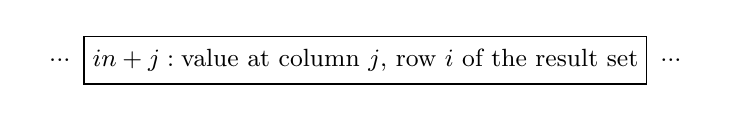
\begin{tikzpicture}
\small
\matrix[nodes={minimum size=6mm}] {
  \node {...};
 &\node[draw] {$in+j:\textrm{value at column $j$, row $i$ of the result set}$};
 &\node {...};\\
};
\end{tikzpicture}

where $i$, $j$ start from 0.\\
\textbf{Side Effects:} none.\\
\textbf{Throws:} {\tt{}SQLException} if database failure is encountered.\\
\bottomrule
\end{tabular}
\nwenddocs{}\nwbegincode{3}\sublabel{NW18ZcDF-3OEpPU-1}\nwmargintag{{\nwtagstyle{}\subpageref{NW18ZcDF-3OEpPU-1}}}\moddef{Read: DBQuery(2)~{\nwtagstyle{}\subpageref{NW18ZcDF-3OEpPU-1}}}\endmoddef\nwused{\\{NW3x1zuR-Oyob-1}}
int[] DBQuery(final String sql, final int ncols) throws SQLException \{
  int[] output = new int[] \{ \};
  try (\LA{}Open \code{}conn\edoc{}~{\nwtagstyle{}\subpageref{NWgUSr6-JT1v9-1}}\RA{}) \{
    Statement stmt = conn.createStatement(
      ResultSet.TYPE_SCROLL_INSENSITIVE, ResultSet.CONCUR_READ_ONLY);
    ResultSet res = stmt.executeQuery(sql);
    if (res.last()) \{
      \LA{}Flatten results~{\nwtagstyle{}\subpageref{NW18ZcDF-3qcw3I-1}}\RA{}
    \}
    conn.close();
  \} catch (SQLException e) \{
    throw e;
  \}
  return output;
\}
\nosublabel{NW18ZcDF-3OEpPU-1-u2}\nwindexdefn{DBQuery}{DBQuery}{NW18ZcDF-3OEpPU-1}\eatline
\nwidentdefs{\\{{DBQuery}{DBQuery}}}\nwendcode{}\nwbegindocs{4}\begin{tabular}{p{\textwidth}}
\toprule
\rowcolor{TableTitle}
Method \textcolor{blue}{{\tt{}\protect\nwindexuse{query}{query}{NW18ZcDF-47dtTX-1}query}}(2) wraps {\tt{}\protect\nwindexuse{DBQuery}{DBQuery}{NW18ZcDF-3OEpPU-1}DBQuery}(2).\\
\bottomrule
\end{tabular}
\nwenddocs{}\nwbegincode{5}\sublabel{NW18ZcDF-47dtTX-1}\nwmargintag{{\nwtagstyle{}\subpageref{NW18ZcDF-47dtTX-1}}}\moddef{Read: query(2)~{\nwtagstyle{}\subpageref{NW18ZcDF-47dtTX-1}}}\endmoddef\nwused{\\{NW3x1zuR-2u8vSA-1}}
int[] query(final String sql, final int ncols) throws SQLException \{
  return this.storage.DBQuery(sql, ncols);
\}
\nwindexdefn{query}{query}{NW18ZcDF-47dtTX-1}\eatline
\nwidentdefs{\\{{query}{query}}}\nwidentuses{\\{{DBQuery}{DBQuery}}}\nwindexuse{DBQuery}{DBQuery}{NW18ZcDF-47dtTX-1}\nwendcode{}\nwbegindocs{6}\nwdocspar
\section{Methods: Read Road Network}

\subsection{\texttt{DBQueryMBR}(0)}
\begin{tabular}{p{\textwidth}}
\toprule
\rowcolor{TableTitle}
Method \textcolor{blue}{{\tt{}\protect\nwindexuse{DBQueryMBR}{DBQueryMBR}{NW18ZcDF-17SWaf-1}DBQueryMBR}}(0) returns the minimum-bounding
rectangle of the road network.
A {\tt{}SQLException} is thrown in case of database failure.\\
\midrule
\textbf{Parameters:} none.\\
\textbf{Returns:} results of the query flattened into an integer array, or
{\tt{}null} if no results.

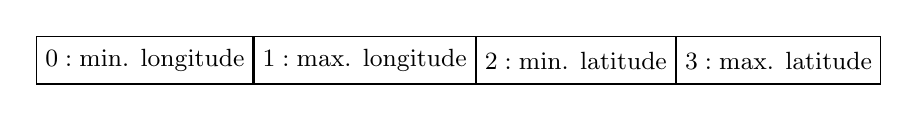
\begin{tikzpicture}
\small
\matrix[nodes={draw,minimum size=6mm}] {
  \node {$0:\textrm{min. longitude}$};
 &\node {$1:\textrm{max. longitude}$};
 &\node {$2:\textrm{min. latitude}$};
 &\node {$3:\textrm{max. latitude}$};\\
};
\end{tikzpicture}\\
\textbf{Side Effects:} none.\\
\textbf{Throws:} {\tt{}SQLException} if database failure is encountered.\\
\bottomrule
\end{tabular}
\nwenddocs{}\nwbegincode{7}\sublabel{NW18ZcDF-17SWaf-1}\nwmargintag{{\nwtagstyle{}\subpageref{NW18ZcDF-17SWaf-1}}}\moddef{Read: DBQueryMBR(0)~{\nwtagstyle{}\subpageref{NW18ZcDF-17SWaf-1}}}\endmoddef\nwused{\\{NW3x1zuR-Oyob-1}}
int[] DBQueryMBR() throws SQLException \{
  try (\LA{}Open \code{}conn\edoc{}~{\nwtagstyle{}\subpageref{NWgUSr6-JT1v9-1}}\RA{}) \{
    return this.PSQuery(conn, "S64", 4);
  \} catch (SQLException e) \{
    throw e;
  \}
\}
\nwindexdefn{DBQueryMBR}{DBQueryMBR}{NW18ZcDF-17SWaf-1}\eatline
\nwidentdefs{\\{{DBQueryMBR}{DBQueryMBR}}}\nwidentuses{\\{{PSQuery}{PSQuery}}\\{{S64}{S64}}}\nwindexuse{PSQuery}{PSQuery}{NW18ZcDF-17SWaf-1}\nwindexuse{S64}{S64}{NW18ZcDF-17SWaf-1}\nwendcode{}\nwbegindocs{8}\begin{tabular}{p{\textwidth}}
\toprule
\rowcolor{TableTitle}
Method \textcolor{blue}{{\tt{}\protect\nwindexuse{queryMBR}{queryMBR}{NW18ZcDF-4JQRjd-1}queryMBR}}(0) wraps {\tt{}\protect\nwindexuse{DBQueryMBR}{DBQueryMBR}{NW18ZcDF-17SWaf-1}DBQueryMBR}(0).\\
\bottomrule
\end{tabular}
\nwenddocs{}\nwbegincode{9}\sublabel{NW18ZcDF-4JQRjd-1}\nwmargintag{{\nwtagstyle{}\subpageref{NW18ZcDF-4JQRjd-1}}}\moddef{Read: queryMBR(0)~{\nwtagstyle{}\subpageref{NW18ZcDF-4JQRjd-1}}}\endmoddef\nwused{\\{NW3x1zuR-2u8vSA-1}}
int[] queryMBR() throws SQLException \{
  return this.storage.DBQueryMBR();
\}
\nwindexdefn{queryMBR}{queryMBR}{NW18ZcDF-4JQRjd-1}\eatline
\nwidentdefs{\\{{queryMBR}{queryMBR}}}\nwidentuses{\\{{DBQueryMBR}{DBQueryMBR}}}\nwindexuse{DBQueryMBR}{DBQueryMBR}{NW18ZcDF-4JQRjd-1}\nwendcode{}\nwbegindocs{10}\nwdocspar
\subsection{\texttt{DBQueryVertex}(1)}
\begin{tabular}{p{\textwidth}}
\toprule
\rowcolor{TableTitle}
Method \textcolor{blue}{{\tt{}\protect\nwindexuse{DBQueryVertex}{DBQueryVertex}{NW18ZcDF-48j64d-1}DBQueryVertex}}(1) returns the longitude and
latitude coordinates of the given vertex. If the vertex does not exist,
a {\tt{}VertexNotFoundException} is thrown.\\
\midrule
\textbf{Parameters:} \\
\begin{tabular}{lp{116mm}}
Integer {\tt{}v} (param. 1):&vertex identifier.
\end{tabular}
\textbf{Returns:} results of the query flattened into an integer array, or
{\tt{}null} if no results.

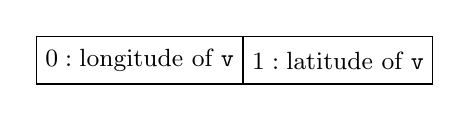
\begin{tikzpicture}
\small
\matrix[nodes={draw,minimum size=6mm}] {
  \node {$0:\textrm{longitude of }\texttt{v}$};
 &\node {$1:\textrm{latitude of }\texttt{v}$};\\
};
\end{tikzpicture}\\
\textbf{Side Effects:} none.\\
\textbf{Throws:} {\tt{}VertexNotFoundException} if vertex does not exist\\
\bottomrule
\end{tabular}
\nwenddocs{}\nwbegincode{11}\sublabel{NW18ZcDF-48j64d-1}\nwmargintag{{\nwtagstyle{}\subpageref{NW18ZcDF-48j64d-1}}}\moddef{Read: DBQueryVertex(1)~{\nwtagstyle{}\subpageref{NW18ZcDF-48j64d-1}}}\endmoddef\nwused{\\{NW3x1zuR-Oyob-1}\\{NW3x1zuR-3QhyAk-1}}
int[] DBQueryVertex(final int v) throws VertexNotFoundException \{
  if (!this.lu_vertices.containsKey(v)) \{
    throw new VertexNotFoundException("Vertex "+v+" not found.");
  \}
  int[] output = this.lu_vertices.get(v).clone();
  return new int[] \{ output[0], output[1], (int) Storage.CSHIFT \};
\}
\nwindexdefn{DBQueryVertex}{DBQueryVertex}{NW18ZcDF-48j64d-1}\eatline
\nwidentdefs{\\{{DBQueryVertex}{DBQueryVertex}}}\nwendcode{}\nwbegindocs{12}\begin{tabular}{p{\textwidth}}
\toprule
\rowcolor{TableTitle}
Method \textcolor{blue}{{\tt{}\protect\nwindexuse{queryVertex}{queryVertex}{NW18ZcDF-oIN5n-1}queryVertex}}(1) wraps {\tt{}\protect\nwindexuse{DBQueryVertex}{DBQueryVertex}{NW18ZcDF-48j64d-1}DBQueryVertex}(1).\\
\bottomrule
\end{tabular}
\nwenddocs{}\nwbegincode{13}\sublabel{NW18ZcDF-oIN5n-1}\nwmargintag{{\nwtagstyle{}\subpageref{NW18ZcDF-oIN5n-1}}}\moddef{Read: queryVertex(1)~{\nwtagstyle{}\subpageref{NW18ZcDF-oIN5n-1}}}\endmoddef\nwused{\\{NW3x1zuR-2u8vSA-1}\\{NW3x1zuR-2Rlctf-1}}
int[] queryVertex(final int v) throws VertexNotFoundException, SQLException \{
  long A0 = System.currentTimeMillis();
  int[] output = this.storage.DBQueryVertex(v);
  \LA{}Stats: queryVertex~{\nwtagstyle{}\subpageref{NW1n2CZQ-49ALld-1}}\RA{}
  return output;
\}
\nosublabel{NW18ZcDF-oIN5n-1-u1}\nwindexdefn{queryVertex}{queryVertex}{NW18ZcDF-oIN5n-1}\eatline
\nwidentdefs{\\{{queryVertex}{queryVertex}}}\nwidentuses{\\{{DBQueryVertex}{DBQueryVertex}}}\nwindexuse{DBQueryVertex}{DBQueryVertex}{NW18ZcDF-oIN5n-1}\nwendcode{}\nwbegindocs{14}\nwdocspar
\subsection{\texttt{DBQueryVertices}(0)}
\begin{tabular}{p{\textwidth}}
\toprule
\rowcolor{TableTitle}
Method \textcolor{blue}{{\tt{}\protect\nwindexuse{DBQueryVertices}{DBQueryVertices}{NW18ZcDF-1imYqa-1}DBQueryVertices}}(0) returns all rows in Table V.
A {\tt{}SQLException} is thrown in case of database failure.\\
\midrule
\textbf{Parameters:} none.\\
\textbf{Returns:} results of the query flattened into an integer array, or
{\tt{}null} if no results.

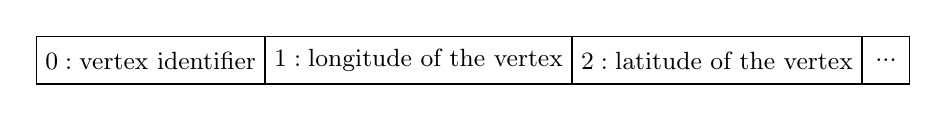
\begin{tikzpicture}
\small
\matrix[nodes={draw,minimum size=6mm}] {
  \node {$0:\textrm{vertex identifier}$};
 &\node {$1:\textrm{longitude of the vertex}$};
 &\node {$2:\textrm{latitude of the vertex}$};
 &\node {...};\\
};
\end{tikzpicture}\\
\textbf{Side Effects:} none.\\
\textbf{Throws:} {\tt{}SQLException} if database failure is encountered.\\
\bottomrule
\end{tabular}
\nwenddocs{}\nwbegincode{15}\sublabel{NW18ZcDF-1imYqa-1}\nwmargintag{{\nwtagstyle{}\subpageref{NW18ZcDF-1imYqa-1}}}\moddef{Read: DBQueryVertices(0)~{\nwtagstyle{}\subpageref{NW18ZcDF-1imYqa-1}}}\endmoddef\nwused{\\{NW3x1zuR-Oyob-1}}
int[] DBQueryVertices() throws SQLException \{
  try (\LA{}Open \code{}conn\edoc{}~{\nwtagstyle{}\subpageref{NWgUSr6-JT1v9-1}}\RA{}) \{
    return this.PSQuery(conn, "S136", 3);
  \} catch (SQLException e) \{
    throw e;
  \}
\}
\nwindexdefn{DBQueryVertices}{DBQueryVertices}{NW18ZcDF-1imYqa-1}\eatline
\nwidentdefs{\\{{DBQueryVertices}{DBQueryVertices}}}\nwidentuses{\\{{PSQuery}{PSQuery}}\\{{S136}{S136}}}\nwindexuse{PSQuery}{PSQuery}{NW18ZcDF-1imYqa-1}\nwindexuse{S136}{S136}{NW18ZcDF-1imYqa-1}\nwendcode{}\nwbegindocs{16}\begin{tabular}{p{\textwidth}}
\toprule
\rowcolor{TableTitle}
Method \textcolor{blue}{{\tt{}\protect\nwindexuse{queryVertices}{queryVertices}{NW18ZcDF-435mrM-1}queryVertices}}(2) wraps {\tt{}\protect\nwindexuse{DBQueryVertices}{DBQueryVertices}{NW18ZcDF-1imYqa-1}DBQueryVertices}(2).\\
\bottomrule
\end{tabular}
\nwenddocs{}\nwbegincode{17}\sublabel{NW18ZcDF-435mrM-1}\nwmargintag{{\nwtagstyle{}\subpageref{NW18ZcDF-435mrM-1}}}\moddef{Read: queryVertices(0)~{\nwtagstyle{}\subpageref{NW18ZcDF-435mrM-1}}}\endmoddef\nwused{\\{NW3x1zuR-2u8vSA-1}}
int[] queryVertices() throws SQLException \{
  return this.storage.DBQueryVertices();
\}
\nwindexdefn{queryVertices}{queryVertices}{NW18ZcDF-435mrM-1}\eatline
\nwidentdefs{\\{{queryVertices}{queryVertices}}}\nwidentuses{\\{{DBQueryVertices}{DBQueryVertices}}}\nwindexuse{DBQueryVertices}{DBQueryVertices}{NW18ZcDF-435mrM-1}\nwendcode{}\nwbegindocs{18}\nwdocspar
\subsection{\texttt{DBQueryVerticesCount}(0)}
\begin{tabular}{p{\textwidth}}
\toprule
\rowcolor{TableTitle}
Method \textcolor{blue}{{\tt{}\protect\nwindexuse{DBQueryVerticesCount}{DBQueryVerticesCount}{NW18ZcDF-1C883O-1}DBQueryVerticesCount}}(0) returns the total number
of vertices in Table V.
A {\tt{}SQLException} is thrown in case of database failure.\\
\midrule
\textbf{Parameters:} none.\\
\textbf{Returns:} results of the query flattened into an integer array, or
{\tt{}null} if no results.

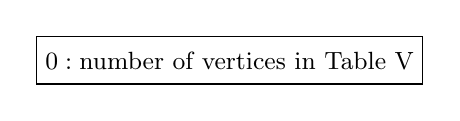
\begin{tikzpicture}
\small
\matrix[nodes={draw,minimum size=6mm}] {
  \node {$0:\textrm{number of vertices in Table V}$};\\
};
\end{tikzpicture}\\
\textbf{Side Effects:} none.\\
\textbf{Throws:} {\tt{}SQLException} if database failure is encountered.\\
\bottomrule
\end{tabular}
\nwenddocs{}\nwbegincode{19}\sublabel{NW18ZcDF-1C883O-1}\nwmargintag{{\nwtagstyle{}\subpageref{NW18ZcDF-1C883O-1}}}\moddef{Read: DBQueryVerticesCount(0)~{\nwtagstyle{}\subpageref{NW18ZcDF-1C883O-1}}}\endmoddef\nwused{\\{NW3x1zuR-Oyob-1}}
int[] DBQueryVerticesCount() throws SQLException \{
  try (\LA{}Open \code{}conn\edoc{}~{\nwtagstyle{}\subpageref{NWgUSr6-JT1v9-1}}\RA{}) \{
    return this.PSQuery(conn, "S62", 1);
  \} catch (SQLException e) \{
    throw e;
  \}
\}
\nwindexdefn{DBQueryVerticesCount}{DBQueryVerticesCount}{NW18ZcDF-1C883O-1}\eatline
\nwidentdefs{\\{{DBQueryVerticesCount}{DBQueryVerticesCount}}}\nwidentuses{\\{{PSQuery}{PSQuery}}\\{{S62}{S62}}}\nwindexuse{PSQuery}{PSQuery}{NW18ZcDF-1C883O-1}\nwindexuse{S62}{S62}{NW18ZcDF-1C883O-1}\nwendcode{}\nwbegindocs{20}\begin{tabular}{p{\textwidth}}
\toprule
\rowcolor{TableTitle}
Method \textcolor{blue}{{\tt{}\protect\nwindexuse{queryVerticesCount}{queryVerticesCount}{NW18ZcDF-EkhgX-1}queryVerticesCount}}(0) wraps {\tt{}\protect\nwindexuse{DBQueryVerticesCount}{DBQueryVerticesCount}{NW18ZcDF-1C883O-1}DBQueryVerticesCount}(0).\\
\bottomrule
\end{tabular}
\nwenddocs{}\nwbegincode{21}\sublabel{NW18ZcDF-EkhgX-1}\nwmargintag{{\nwtagstyle{}\subpageref{NW18ZcDF-EkhgX-1}}}\moddef{Read: queryVerticesCount(0)~{\nwtagstyle{}\subpageref{NW18ZcDF-EkhgX-1}}}\endmoddef\nwused{\\{NW3x1zuR-2u8vSA-1}}
int[] queryVerticesCount() throws SQLException \{
  return this.storage.DBQueryVerticesCount();
\}
\nwindexdefn{queryVerticesCount}{queryVerticesCount}{NW18ZcDF-EkhgX-1}\eatline
\nwidentdefs{\\{{queryVerticesCount}{queryVerticesCount}}}\nwidentuses{\\{{DBQueryVerticesCount}{DBQueryVerticesCount}}}\nwindexuse{DBQueryVerticesCount}{DBQueryVerticesCount}{NW18ZcDF-EkhgX-1}\nwendcode{}\nwbegindocs{22}\nwdocspar
\subsection{\texttt{DBQueryEdge}(2)}
\begin{tabular}{p{\textwidth}}
\toprule
\rowcolor{TableTitle}
Method \textcolor{blue}{{\tt{}\protect\nwindexuse{DBQueryEdge}{DBQueryEdge}{NW18ZcDF-1eCWox-1}DBQueryEdge}}(2) returns the distance and
maximum free-flow speed along the given edge.
An {\tt{}EdgeNotFoundException} is thrown if the edge does not exist.\\
\midrule
\textbf{Parameters:} \\
\begin{tabular}{lp{116mm}}
Integer {\tt{}v1} (param. 1):&source vertex identifier $v_1$\\
Integer {\tt{}v2} (param. 2):&target vertex identifier $v_2$
\end{tabular}\\
\textbf{Returns:} results of the query flattened into an integer array, or
{\tt{}null} if no results.

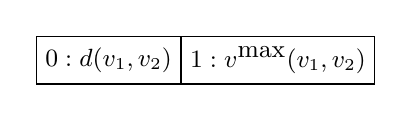
\begin{tikzpicture}
\small
\matrix[nodes={draw,minimum size=6mm}] {
  \node {$0:d(v_1,v_2)$}; & \node {$1:v^\textrm{max}(v_1,v_2)$}; \\
};
\end{tikzpicture}\\
\textbf{Side Effects:} none.\\
\textbf{Throws:} {\tt{}EdgeNotFoundException} if edge does not exit.\\
\bottomrule
\end{tabular}
\nwenddocs{}\nwbegincode{23}\sublabel{NW18ZcDF-1eCWox-1}\nwmargintag{{\nwtagstyle{}\subpageref{NW18ZcDF-1eCWox-1}}}\moddef{Read: DBQueryEdge(2)~{\nwtagstyle{}\subpageref{NW18ZcDF-1eCWox-1}}}\endmoddef\nwused{\\{NW3x1zuR-Oyob-1}\\{NW3x1zuR-3QhyAk-1}}
int[] DBQueryEdge(final int v1, final int v2) throws EdgeNotFoundException \{
  if (!(this.lu_edges.containsKey(v1) && this.lu_edges.get(v1).containsKey(v2))) \{
    throw new EdgeNotFoundException("Edge ("+v1+", "+v2+") not found.");
  \}
  return this.lu_edges.get(v1).get(v2).clone();
\}
\nwindexdefn{DBQueryEdge}{DBQueryEdge}{NW18ZcDF-1eCWox-1}\eatline
\nwidentdefs{\\{{DBQueryEdge}{DBQueryEdge}}}\nwendcode{}\nwbegindocs{24}\begin{tabular}{p{\textwidth}}
\toprule
\rowcolor{TableTitle}
Method \textcolor{blue}{{\tt{}\protect\nwindexuse{queryEdge}{queryEdge}{NW18ZcDF-1H3Dhp-1}queryEdge}}(2) wraps {\tt{}\protect\nwindexuse{DBQueryEdge}{DBQueryEdge}{NW18ZcDF-1eCWox-1}DBQueryEdge}(2).\\
\bottomrule
\end{tabular}
\nwenddocs{}\nwbegincode{25}\sublabel{NW18ZcDF-1H3Dhp-1}\nwmargintag{{\nwtagstyle{}\subpageref{NW18ZcDF-1H3Dhp-1}}}\moddef{Read: queryEdge(2)~{\nwtagstyle{}\subpageref{NW18ZcDF-1H3Dhp-1}}}\endmoddef\nwused{\\{NW3x1zuR-2u8vSA-1}\\{NW3x1zuR-2Rlctf-1}}
int[] queryEdge(final int v1, final int v2) throws EdgeNotFoundException, SQLException \{
  long A0 = System.currentTimeMillis();
  int[] output = this.storage.DBQueryEdge(v1, v2);
  \LA{}Stats: queryEdge~{\nwtagstyle{}\subpageref{NW1n2CZQ-FCg3E-1}}\RA{}
  return output;
\}
\nosublabel{NW18ZcDF-1H3Dhp-1-u1}\nwindexdefn{queryEdge}{queryEdge}{NW18ZcDF-1H3Dhp-1}\eatline
\nwidentdefs{\\{{queryEdge}{queryEdge}}}\nwidentuses{\\{{DBQueryEdge}{DBQueryEdge}}}\nwindexuse{DBQueryEdge}{DBQueryEdge}{NW18ZcDF-1H3Dhp-1}\nwendcode{}\nwbegindocs{26}\nwdocspar
\subsection{\texttt{DBQueryEdges}(0)}
\begin{tabular}{p{\textwidth}}
\toprule
\rowcolor{TableTitle}
Method \textcolor{blue}{{\tt{}\protect\nwindexuse{DBQueryEdges}{DBQueryEdges}{NW18ZcDF-1uCRXX-1}DBQueryEdges}}(0) returns all rows in Table E.
A {\tt{}SQLException} is thrown in case of database failure.\\
\midrule
\textbf{Parameters:} none.\\
\textbf{Returns:} results of the query flattened into an integer array, or
{\tt{}null} if no results.

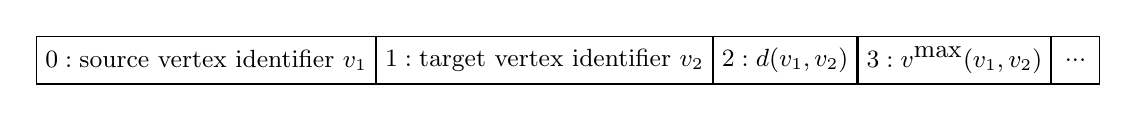
\begin{tikzpicture}
\small
\matrix[nodes={draw,minimum size=6mm}] {
  \node {$0:\textrm{source vertex identifier $v_1$}$};
 &\node {$1:\textrm{target vertex identifier $v_2$}$};
 &\node {$2:d(v_1,v_2)$};
 &\node {$3:v^\textrm{max}(v_1,v_2)$};
 &\node {...};\\
};
\end{tikzpicture}\\
\textbf{Side Effects:} none.\\
\textbf{Throws:} {\tt{}SQLException} if database failure is encountered.\\
\bottomrule
\end{tabular}
\nwenddocs{}\nwbegincode{27}\sublabel{NW18ZcDF-1uCRXX-1}\nwmargintag{{\nwtagstyle{}\subpageref{NW18ZcDF-1uCRXX-1}}}\moddef{Read: DBQueryEdges(0)~{\nwtagstyle{}\subpageref{NW18ZcDF-1uCRXX-1}}}\endmoddef\nwused{\\{NW3x1zuR-Oyob-1}}
int[] DBQueryEdges() throws SQLException \{
  try (\LA{}Open \code{}conn\edoc{}~{\nwtagstyle{}\subpageref{NWgUSr6-JT1v9-1}}\RA{}) \{
    return this.PSQuery(conn, "S137", 4);
  \} catch (SQLException e) \{
    throw e;
  \}
\}
\nwindexdefn{DBQueryEdges}{DBQueryEdges}{NW18ZcDF-1uCRXX-1}\eatline
\nwidentdefs{\\{{DBQueryEdges}{DBQueryEdges}}}\nwidentuses{\\{{PSQuery}{PSQuery}}\\{{S137}{S137}}}\nwindexuse{PSQuery}{PSQuery}{NW18ZcDF-1uCRXX-1}\nwindexuse{S137}{S137}{NW18ZcDF-1uCRXX-1}\nwendcode{}\nwbegindocs{28}\begin{tabular}{p{\textwidth}}
\toprule
\rowcolor{TableTitle}
Method \textcolor{blue}{{\tt{}\protect\nwindexuse{queryEdges}{queryEdges}{NW18ZcDF-14B11a-1}queryEdges}}(2) wraps {\tt{}\protect\nwindexuse{DBQueryEdges}{DBQueryEdges}{NW18ZcDF-1uCRXX-1}DBQueryEdges}(2).\\
\bottomrule
\end{tabular}
\nwenddocs{}\nwbegincode{29}\sublabel{NW18ZcDF-14B11a-1}\nwmargintag{{\nwtagstyle{}\subpageref{NW18ZcDF-14B11a-1}}}\moddef{Read: queryEdges(0)~{\nwtagstyle{}\subpageref{NW18ZcDF-14B11a-1}}}\endmoddef\nwused{\\{NW3x1zuR-2u8vSA-1}}
int[] queryEdges() throws SQLException \{
  return this.storage.DBQueryEdges();
\}
\nwindexdefn{queryEdges}{queryEdges}{NW18ZcDF-14B11a-1}\eatline
\nwidentdefs{\\{{queryEdges}{queryEdges}}}\nwidentuses{\\{{DBQueryEdges}{DBQueryEdges}}}\nwindexuse{DBQueryEdges}{DBQueryEdges}{NW18ZcDF-14B11a-1}\nwendcode{}\nwbegindocs{30}\nwdocspar
\subsection{\texttt{DBQueryEdgesCount}(0)}
\begin{tabular}{p{\textwidth}}
\toprule
\rowcolor{TableTitle}
Method \textcolor{blue}{{\tt{}\protect\nwindexuse{DBQueryEdgesCount}{DBQueryEdgesCount}{NW18ZcDF-4bU7WY-1}DBQueryEdgesCount}}(0) returns the total number
of vertices in Table V.
A {\tt{}SQLException} is thrown in case of database failure.\\
\midrule
\textbf{Parameters:} none.\\
\textbf{Returns:} results of the query flattened into an integer array, or
{\tt{}null} if no results.

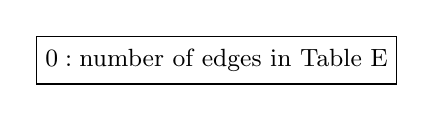
\begin{tikzpicture}
\small
\matrix[nodes={draw,minimum size=6mm}] {
  \node {$0:\textrm{number of edges in Table E}$};\\
};
\end{tikzpicture}\\
\textbf{Side Effects:} none.\\
\textbf{Throws:} {\tt{}SQLException} if database failure is encountered.\\
\bottomrule
\end{tabular}
\nwenddocs{}\nwbegincode{31}\sublabel{NW18ZcDF-4bU7WY-1}\nwmargintag{{\nwtagstyle{}\subpageref{NW18ZcDF-4bU7WY-1}}}\moddef{Read: DBQueryEdgesCount(0)~{\nwtagstyle{}\subpageref{NW18ZcDF-4bU7WY-1}}}\endmoddef\nwused{\\{NW3x1zuR-Oyob-1}}
int[] DBQueryEdgesCount() throws SQLException \{
  try (\LA{}Open \code{}conn\edoc{}~{\nwtagstyle{}\subpageref{NWgUSr6-JT1v9-1}}\RA{}) \{
    return this.PSQuery(conn, "S63", 1);
  \} catch (SQLException e) \{
    throw e;
  \}
\}
\nwindexdefn{DBQueryEdgesCount}{DBQueryEdgesCount}{NW18ZcDF-4bU7WY-1}\eatline
\nwidentdefs{\\{{DBQueryEdgesCount}{DBQueryEdgesCount}}}\nwidentuses{\\{{PSQuery}{PSQuery}}\\{{S63}{S63}}}\nwindexuse{PSQuery}{PSQuery}{NW18ZcDF-4bU7WY-1}\nwindexuse{S63}{S63}{NW18ZcDF-4bU7WY-1}\nwendcode{}\nwbegindocs{32}\begin{tabular}{p{\textwidth}}
\toprule
\rowcolor{TableTitle}
Method \textcolor{blue}{{\tt{}\protect\nwindexuse{queryEdgesCount}{queryEdgesCount}{NW18ZcDF-3fg08d-1}queryEdgesCount}}(0) wraps {\tt{}\protect\nwindexuse{DBQueryEdgesCount}{DBQueryEdgesCount}{NW18ZcDF-4bU7WY-1}DBQueryEdgesCount}(0).\\
\bottomrule
\end{tabular}
\nwenddocs{}\nwbegincode{33}\sublabel{NW18ZcDF-3fg08d-1}\nwmargintag{{\nwtagstyle{}\subpageref{NW18ZcDF-3fg08d-1}}}\moddef{Read: queryEdgesCount(0)~{\nwtagstyle{}\subpageref{NW18ZcDF-3fg08d-1}}}\endmoddef\nwused{\\{NW3x1zuR-2u8vSA-1}}
int[] queryEdgesCount() throws SQLException \{
  return this.storage.DBQueryEdgesCount();
\}
\nwindexdefn{queryEdgesCount}{queryEdgesCount}{NW18ZcDF-3fg08d-1}\eatline
\nwidentdefs{\\{{queryEdgesCount}{queryEdgesCount}}}\nwidentuses{\\{{DBQueryEdgesCount}{DBQueryEdgesCount}}}\nwindexuse{DBQueryEdgesCount}{DBQueryEdgesCount}{NW18ZcDF-3fg08d-1}\nwendcode{}\nwbegindocs{34}\nwdocspar
\subsection{\texttt{DBQueryEdgeStatistics}(0)}
\begin{tabular}{p{\textwidth}}
\toprule
\rowcolor{TableTitle}
Method \textcolor{blue}{{\tt{}\protect\nwindexuse{DBQueryEdgeStatistics}{DBQueryEdgeStatistics}{NW18ZcDF-3w6nA9-1}DBQueryEdgeStatistics}}(0) returns some edge statistics.
A {\tt{}SQLException} is thrown in case of database failure.\\
\midrule
\textbf{Parameters:} none.\\
\textbf{Returns:} results of the query flattened into an integer array, or
{\tt{}null} if no results.

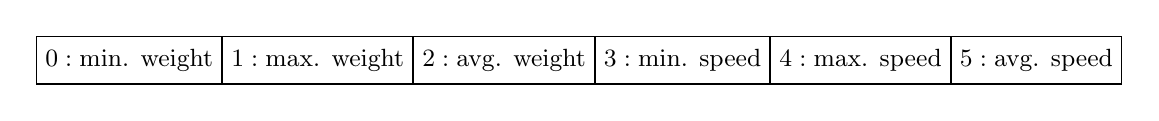
\begin{tikzpicture}
\small
\matrix[nodes={draw,minimum size=6mm}] {
  \node {$0:\textrm{min. weight}$};
 &\node {$1:\textrm{max. weight}$};
 &\node {$2:\textrm{avg. weight}$};
 &\node {$3:\textrm{min. speed}$};
 &\node {$4:\textrm{max. speed}$};
 &\node {$5:\textrm{avg. speed}$};\\
};
\end{tikzpicture}\\
\textbf{Side Effects:} none.\\
\textbf{Throws:} {\tt{}SQLException} if database failure is encountered.\\
\bottomrule
\end{tabular}
\nwenddocs{}\nwbegincode{35}\sublabel{NW18ZcDF-3w6nA9-1}\nwmargintag{{\nwtagstyle{}\subpageref{NW18ZcDF-3w6nA9-1}}}\moddef{Read: DBQueryEdgeStatistics(0)~{\nwtagstyle{}\subpageref{NW18ZcDF-3w6nA9-1}}}\endmoddef\nwused{\\{NW3x1zuR-Oyob-1}}
int[] DBQueryEdgeStatistics() throws SQLException \{
  try (\LA{}Open \code{}conn\edoc{}~{\nwtagstyle{}\subpageref{NWgUSr6-JT1v9-1}}\RA{}) \{
    return this.PSQuery(conn, "S65", 6);
  \} catch (SQLException e) \{
    throw e;
  \}
\}
\nwindexdefn{DBQueryEdgeStatistics}{DBQueryEdgeStatistics}{NW18ZcDF-3w6nA9-1}\eatline
\nwidentdefs{\\{{DBQueryEdgeStatistics}{DBQueryEdgeStatistics}}}\nwidentuses{\\{{PSQuery}{PSQuery}}\\{{S65}{S65}}}\nwindexuse{PSQuery}{PSQuery}{NW18ZcDF-3w6nA9-1}\nwindexuse{S65}{S65}{NW18ZcDF-3w6nA9-1}\nwendcode{}\nwbegindocs{36}\nwdocspar
\section{Methods: Read User Properties}

\subsection{\texttt{DBQueryUser}(1)}
\begin{tabular}{p{\textwidth}}
\toprule
\rowcolor{TableTitle}
Method \textcolor{blue}{{\tt{}\protect\nwindexuse{DBQueryUser}{DBQueryUser}{NW18ZcDF-8IJdE-1}DBQueryUser}}(0) returns the properties of the
given user.
A {\tt{}UserNotFoundException} is thrown if the user does not exist.\\
\midrule
\textbf{Parameters:} \\
\begin{tabular}{lp{116mm}}
Integer {\tt{}uid} (param. 1):&user identifier for user $u$
\end{tabular}
\textbf{Returns:} results of the query flattened into an integer array, or
{\tt{}null} if no results.

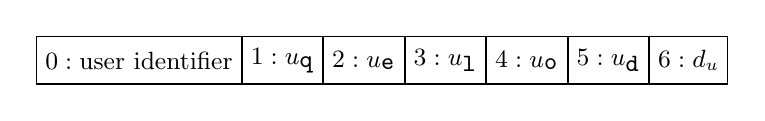
\begin{tikzpicture}
\small
\matrix[nodes={draw,minimum size=6mm}] {
  \node {$0:\textrm{user identifier}$};
 &\node {$1:u_\texttt{q}$};
 &\node {$2:u_\texttt{e}$};
 &\node {$3:u_\texttt{l}$};
 &\node {$4:u_\texttt{o}$};
 &\node {$5:u_\texttt{d}$};
 &\node {$6:d_u$};\\
};
\end{tikzpicture}\\
\textbf{Side Effects:} none.\\
\textbf{Throws:} {\tt{}UserNotFoundException} if user does not exist.\\
\bottomrule
\end{tabular}
\nwenddocs{}\nwbegincode{37}\sublabel{NW18ZcDF-8IJdE-1}\nwmargintag{{\nwtagstyle{}\subpageref{NW18ZcDF-8IJdE-1}}}\moddef{Read: DBQueryUser(1)~{\nwtagstyle{}\subpageref{NW18ZcDF-8IJdE-1}}}\endmoddef\nwused{\\{NW3x1zuR-Oyob-1}}
int[] DBQueryUser(final int uid)
throws UserNotFoundException \{
  if (!this.lu_users.containsKey(uid)) \{
    throw new UserNotFoundException("User "+uid+" not found.");
  \}
  return this.lu_users.get(uid).clone();
\}
\nwindexdefn{DBQueryUser}{DBQueryUser}{NW18ZcDF-8IJdE-1}\eatline
\nwidentdefs{\\{{DBQueryUser}{DBQueryUser}}}\nwendcode{}\nwbegindocs{38}\begin{tabular}{p{\textwidth}}
\toprule
\rowcolor{TableTitle}
Method \textcolor{blue}{{\tt{}\protect\nwindexuse{queryUser}{queryUser}{NW18ZcDF-SBVOE-1}queryUser}}(1) wraps {\tt{}\protect\nwindexuse{DBQueryUser}{DBQueryUser}{NW18ZcDF-8IJdE-1}DBQueryUser}(1).\\
\bottomrule
\end{tabular}
\nwenddocs{}\nwbegincode{39}\sublabel{NW18ZcDF-SBVOE-1}\nwmargintag{{\nwtagstyle{}\subpageref{NW18ZcDF-SBVOE-1}}}\moddef{Read: queryUser(1)~{\nwtagstyle{}\subpageref{NW18ZcDF-SBVOE-1}}}\endmoddef\nwused{\\{NW3x1zuR-2u8vSA-1}\\{NW3x1zuR-2Rlctf-1}}
int[] queryUser(final int rid) throws UserNotFoundException, SQLException \{
  long A0 = System.currentTimeMillis();
  int[] output = storage.DBQueryUser(rid);
  \LA{}Stats: queryUser~{\nwtagstyle{}\subpageref{NW1n2CZQ-3RV80d-1}}\RA{}
  return output;
\}
\nosublabel{NW18ZcDF-SBVOE-1-u1}\nwindexdefn{queryUser}{queryUser}{NW18ZcDF-SBVOE-1}\eatline
\nwidentdefs{\\{{queryUser}{queryUser}}}\nwidentuses{\\{{DBQueryUser}{DBQueryUser}}}\nwindexuse{DBQueryUser}{DBQueryUser}{NW18ZcDF-SBVOE-1}\nwendcode{}\nwbegindocs{40}\nwdocspar
\subsection{\texttt{DBQueryUsers}(0)}
\begin{tabular}{p{\textwidth}}
\toprule
\rowcolor{TableTitle}
Method \textcolor{blue}{{\tt{}\protect\nwindexuse{DBQueryUsers}{DBQueryUsers}{NW18ZcDF-4dNZxZ-1}DBQueryUsers}}(0) returns all rows in view {\tt{}r{\char95}user}.
A {\tt{}SQLException} is thrown in case of database failure.\\
\midrule
\textbf{Parameters:} none.\\
\textbf{Returns:} results of the query flattened into an integer array, or
{\tt{}null} if no results.

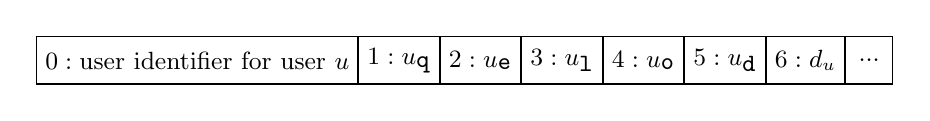
\begin{tikzpicture}
\small
\matrix[nodes={draw,minimum size=6mm}] {
  \node {$0:\textrm{user identifier for user $u$}$};
 &\node {$1:u_\texttt{q}$};
 &\node {$2:u_\texttt{e}$};
 &\node {$3:u_\texttt{l}$};
 &\node {$4:u_\texttt{o}$};
 &\node {$5:u_\texttt{d}$};
 &\node {$6:d_u$};
 &\node {...};\\
};
\end{tikzpicture}\\
\textbf{Side Effects:} none.\\
\textbf{Throws:} {\tt{}SQLException} if database failure is encountered.\\
\bottomrule
\end{tabular}
\nwenddocs{}\nwbegincode{41}\sublabel{NW18ZcDF-4dNZxZ-1}\nwmargintag{{\nwtagstyle{}\subpageref{NW18ZcDF-4dNZxZ-1}}}\moddef{Read: DBQueryUsers(0)~{\nwtagstyle{}\subpageref{NW18ZcDF-4dNZxZ-1}}}\endmoddef\nwused{\\{NW3x1zuR-Oyob-1}}
int[] DBQueryUsers() throws SQLException \{
  try (\LA{}Open \code{}conn\edoc{}~{\nwtagstyle{}\subpageref{NWgUSr6-JT1v9-1}}\RA{}) \{
    return this.PSQuery(conn, "S141", 7);
  \} catch (SQLException e) \{
    throw e;
  \}
\}
\nwindexdefn{DBQueryUsers}{DBQueryUsers}{NW18ZcDF-4dNZxZ-1}\eatline
\nwidentdefs{\\{{DBQueryUsers}{DBQueryUsers}}}\nwidentuses{\\{{PSQuery}{PSQuery}}\\{{S141}{S141}}}\nwindexuse{PSQuery}{PSQuery}{NW18ZcDF-4dNZxZ-1}\nwindexuse{S141}{S141}{NW18ZcDF-4dNZxZ-1}\nwendcode{}\nwbegindocs{42}\nwdocspar
\subsection{\texttt{DBQueryRequestStatus}(2)}
\begin{tabular}{p{\textwidth}}
\toprule
\rowcolor{TableTitle}
Method \textcolor{blue}{{\tt{}\protect\nwindexuse{DBQueryRequestStatus}{DBQueryRequestStatus}{NW18ZcDF-2bbv1T-1}DBQueryRequestStatus}}(0) returns the status of
the given request at the given time (Eq.~\ref{eq:status}).
A {\tt{}UserNotFoundException} is thrown if the user does not exist.
A {\tt{}SQLException} is thrown in case of database failure.\\
\midrule
\textbf{Parameters:} \\
\begin{tabular}{lp{116mm}}
Integer {\tt{}rid} (param. 1):&user identifier for request $r$\\
Integer {\tt{}t} (param. 2):&a time
\end{tabular}\\
\textbf{Returns:} results of the query flattened into an integer array, or
{\tt{}null} if no results.

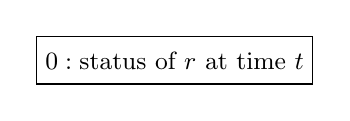
\begin{tikzpicture}
\small
\matrix[nodes={draw,minimum size=6mm}] {
  \node {$0:\textrm{status of $r$ at time $t$}$};\\
};
\end{tikzpicture}\\
\textbf{Side Effects:} none.\\
\textbf{Throws:} {\tt{}UserNotFoundException} if user does not exist, or
{\tt{}SQLException} if database failure is encountered.\\
\bottomrule
\end{tabular}
\nwenddocs{}\nwbegincode{43}\sublabel{NW18ZcDF-2bbv1T-1}\nwmargintag{{\nwtagstyle{}\subpageref{NW18ZcDF-2bbv1T-1}}}\moddef{Read: DBQueryRequestStatus(2)~{\nwtagstyle{}\subpageref{NW18ZcDF-2bbv1T-1}}}\endmoddef\nwused{\\{NW3x1zuR-Oyob-1}}
int[] DBQueryRequestStatus(final int rid, final int t)
throws UserNotFoundException, SQLException \{
  if (!this.lu_users.containsKey(rid)) \{
    throw new UserNotFoundException("User "+rid+" not found.");
  \}
  try (\LA{}Open \code{}conn\edoc{}~{\nwtagstyle{}\subpageref{NWgUSr6-JT1v9-1}}\RA{}) \{
    return this.PSQuery(conn, "S133", 1, rid, t);
  \} catch (SQLException e) \{
    throw e;
  \}
\}
\nwindexdefn{DBQueryRequestStatus}{DBQueryRequestStatus}{NW18ZcDF-2bbv1T-1}\eatline
\nwidentdefs{\\{{DBQueryRequestStatus}{DBQueryRequestStatus}}}\nwidentuses{\\{{PSQuery}{PSQuery}}\\{{S133}{S133}}}\nwindexuse{PSQuery}{PSQuery}{NW18ZcDF-2bbv1T-1}\nwindexuse{S133}{S133}{NW18ZcDF-2bbv1T-1}\nwendcode{}\nwbegindocs{44}\begin{tabular}{p{\textwidth}}
\toprule
\rowcolor{TableTitle}
Method \textcolor{blue}{{\tt{}\protect\nwindexuse{queryEdgeStatistics}{queryEdgeStatistics}{NW18ZcDF-1SAYMv-1}queryEdgeStatistics}}(0) wraps {\tt{}\protect\nwindexuse{DBQueryEdgeStatistics}{DBQueryEdgeStatistics}{NW18ZcDF-3w6nA9-1}DBQueryEdgeStatistics}(0).\\
\bottomrule
\end{tabular}
\nwenddocs{}\nwbegincode{45}\sublabel{NW18ZcDF-1SAYMv-1}\nwmargintag{{\nwtagstyle{}\subpageref{NW18ZcDF-1SAYMv-1}}}\moddef{Read: queryEdgeStatistics(0)~{\nwtagstyle{}\subpageref{NW18ZcDF-1SAYMv-1}}}\endmoddef\nwused{\\{NW3x1zuR-2u8vSA-1}}
int[] queryEdgeStatistics() throws SQLException \{
  return storage.DBQueryEdgeStatistics();
\}
\nwindexdefn{queryEdgeStatistics}{queryEdgeStatistics}{NW18ZcDF-1SAYMv-1}\eatline
\nwidentdefs{\\{{queryEdgeStatistics}{queryEdgeStatistics}}}\nwidentuses{\\{{DBQueryEdgeStatistics}{DBQueryEdgeStatistics}}}\nwindexuse{DBQueryEdgeStatistics}{DBQueryEdgeStatistics}{NW18ZcDF-1SAYMv-1}\nwendcode{}\nwbegindocs{46}\nwdocspar
\subsection{\texttt{DBQueryRequestIsAssigned}(1)}
\begin{tabular}{p{\textwidth}}
\toprule
\rowcolor{TableTitle}
Method \textcolor{blue}{{\tt{}\protect\nwindexuse{DBQueryRequestIsAssigned}{DBQueryRequestIsAssigned}{NW18ZcDF-1ZOEl0-1}DBQueryRequestIsAssigned}}(1) returns a
positive-length array if the given request is assigned (even if the request is
not yet picked-up), or {\tt{}null} if the request is not.  A
{\tt{}UserNotFoundException} is thrown if the user does not exist.
A {\tt{}SQLException} is thrown in case of database failure.\\
\midrule
\textbf{Parameters:} \\
\begin{tabular}{lp{116mm}}
Integer {\tt{}rid} (param. 1):&user identifier for request $r$
\end{tabular}\\
\textbf{Returns:} results of the query flattened into an integer array, or
{\tt{}null} if no results.

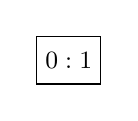
\begin{tikzpicture}
\small
\matrix[nodes={draw,minimum size=6mm}] {
  \node {$0:1$};\\
};
\end{tikzpicture}\\
\textbf{Side Effects:} none.\\
\textbf{Throws:} {\tt{}UserNotFoundException} if user does not exist, or
{\tt{}SQLException} if database failure is encountered.\\
\bottomrule
\end{tabular}
\nwenddocs{}\nwbegincode{47}\sublabel{NW18ZcDF-1ZOEl0-1}\nwmargintag{{\nwtagstyle{}\subpageref{NW18ZcDF-1ZOEl0-1}}}\moddef{Read: DBQueryRequestIsAssigned(1)~{\nwtagstyle{}\subpageref{NW18ZcDF-1ZOEl0-1}}}\endmoddef\nwused{\\{NW3x1zuR-Oyob-1}}
int[] DBQueryRequestIsAssigned(final int rid) throws SQLException \{
  try (\LA{}Open \code{}conn\edoc{}~{\nwtagstyle{}\subpageref{NWgUSr6-JT1v9-1}}\RA{}) \{
    return this.PSQuery(conn, "S148", 1, rid);
  \} catch (SQLException e) \{
    throw e;
  \}
\}
\nwindexdefn{DBQueryRequestIsAssigned}{DBQueryRequestIsAssigned}{NW18ZcDF-1ZOEl0-1}\eatline
\nwidentdefs{\\{{DBQueryRequestIsAssigned}{DBQueryRequestIsAssigned}}}\nwidentuses{\\{{PSQuery}{PSQuery}}\\{{S148}{S148}}}\nwindexuse{PSQuery}{PSQuery}{NW18ZcDF-1ZOEl0-1}\nwindexuse{S148}{S148}{NW18ZcDF-1ZOEl0-1}\nwendcode{}\nwbegindocs{48}\nwdocspar
\subsection{\texttt{DBQueryRequestDistanceDetour}(1)}
\begin{tabular}{p{\textwidth}}
\toprule
\rowcolor{TableTitle}
Method \textcolor{blue}{{\tt{}\protect\nwindexuse{DBQueryRequestDistanceDetour}{DBQueryRequestDistanceDetour}{NW18ZcDF-3Jk4Pm-1}DBQueryRequestDistanceDetour}}(1) returns the
detour distance $D^\textrm{detour}(\mathcal{X},r)$
(Eq.~\ref{eq:detour-distance}) of the given request.
A {\tt{}SQLException} is thrown in case of database failure.\\
\midrule
\textbf{Parameters:}\\
\begin{tabular}{lp{116mm}}
Integer {\tt{}rid} (param. 1):&request identifier.
\end{tabular}\\
\textbf{Returns:} results of the query flattened into an integer array,
or {\tt{}null} if no results.

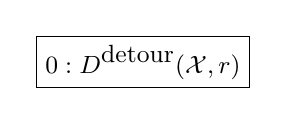
\begin{tikzpicture}
\small
\matrix[nodes={minimum size=6mm}] {
  \node[draw] {$0:D^\textrm{detour}(\mathcal{X},r)$};\\
};
\end{tikzpicture}

where $r$ is the request identified by {\tt{}rid} (param. 1).\\
\textbf{Side Effects:} none.\\
\textbf{Throws:} {\tt{}SQLException} if database failure is encountered.\\
\bottomrule
\end{tabular}
\nwenddocs{}\nwbegincode{49}\sublabel{NW18ZcDF-3Jk4Pm-1}\nwmargintag{{\nwtagstyle{}\subpageref{NW18ZcDF-3Jk4Pm-1}}}\moddef{Read: DBQueryRequestDistanceDetour(1)~{\nwtagstyle{}\subpageref{NW18ZcDF-3Jk4Pm-1}}}\endmoddef\nwused{\\{NW3x1zuR-Oyob-1}}
int[] DBQueryRequestDistanceDetour(final int rid) throws SQLException \{
  try (\LA{}Open \code{}conn\edoc{}~{\nwtagstyle{}\subpageref{NWgUSr6-JT1v9-1}}\RA{}) \{
    return PSQuery(conn, "S112", 1, rid);
  \} catch (SQLException e) \{
    throw e;
  \}
\}
\nwindexdefn{DBQueryRequestDistanceDetour}{DBQueryRequestDistanceDetour}{NW18ZcDF-3Jk4Pm-1}\eatline
\nwidentdefs{\\{{DBQueryRequestDistanceDetour}{DBQueryRequestDistanceDetour}}}\nwidentuses{\\{{PSQuery}{PSQuery}}\\{{S112}{S112}}}\nwindexuse{PSQuery}{PSQuery}{NW18ZcDF-3Jk4Pm-1}\nwindexuse{S112}{S112}{NW18ZcDF-3Jk4Pm-1}\nwendcode{}\nwbegindocs{50}\nwdocspar
\subsection{\texttt{DBQueryRequestDistanceTransit}(1)}
\begin{tabular}{p{\textwidth}}
\toprule
\rowcolor{TableTitle}
Method \textcolor{blue}{{\tt{}\protect\nwindexuse{DBQueryRequestDistanceTransit}{DBQueryRequestDistanceTransit}{NW18ZcDF-4808iY-1}DBQueryRequestDistanceTransit}}(1) returns the
transit distance $D^\textrm{transit}(\mathcal{X},r)$
(Eq.~\ref{eq:transit-distance}) of the given request.
A {\tt{}SQLException} is thrown in case of database failure.\\
\midrule
\textbf{Parameters:}\\
\begin{tabular}{lp{116mm}}
Integer {\tt{}rid} (param. 1):&request identifier.
\end{tabular}\\
\textbf{Returns:} results of the query flattened into an integer array,
or {\tt{}null} if no results.

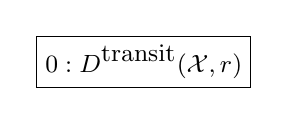
\begin{tikzpicture}
\small
\matrix[nodes={minimum size=6mm}] {
  \node[draw] {$0:D^\textrm{transit}(\mathcal{X},r)$};\\
};
\end{tikzpicture}

where $r$ is the request identified by {\tt{}rid} (param. 1).\\
\textbf{Side Effects:} none.\\
\textbf{Throws:} {\tt{}SQLException} if database failure is encountered.\\
\bottomrule
\end{tabular}
\nwenddocs{}\nwbegincode{51}\sublabel{NW18ZcDF-4808iY-1}\nwmargintag{{\nwtagstyle{}\subpageref{NW18ZcDF-4808iY-1}}}\moddef{Read: DBQueryRequestDistanceTransit(1)~{\nwtagstyle{}\subpageref{NW18ZcDF-4808iY-1}}}\endmoddef\nwused{\\{NW3x1zuR-Oyob-1}}
int[] DBQueryRequestDistanceTransit(final int rid) throws SQLException \{
  try (\LA{}Open \code{}conn\edoc{}~{\nwtagstyle{}\subpageref{NWgUSr6-JT1v9-1}}\RA{}) \{
    return PSQuery(conn, "S114", 1, rid);
  \} catch (SQLException e) \{
    throw e;
  \}
\}
\nwindexdefn{DBQueryRequestDistanceTransit}{DBQueryRequestDistanceTransit}{NW18ZcDF-4808iY-1}\eatline
\nwidentdefs{\\{{DBQueryRequestDistanceTransit}{DBQueryRequestDistanceTransit}}}\nwidentuses{\\{{PSQuery}{PSQuery}}\\{{S114}{S114}}}\nwindexuse{PSQuery}{PSQuery}{NW18ZcDF-4808iY-1}\nwindexuse{S114}{S114}{NW18ZcDF-4808iY-1}\nwendcode{}\nwbegindocs{52}\nwdocspar
\subsection{\texttt{DBQueryRequestDurationPickup}(1)}
\begin{tabular}{p{\textwidth}}
\toprule
\rowcolor{TableTitle}
Method \textcolor{blue}{{\tt{}\protect\nwindexuse{DBQueryRequestDurationPickup}{DBQueryRequestDurationPickup}{NW18ZcDF-3eqIl6-1}DBQueryRequestDurationPickup}}(1) returns the
pickup delay $\delta^\textrm{pickup}(\mathcal{X},r)$
(Eq.~\ref{eq:pick-up delay}) of the given request.
A {\tt{}SQLException} is thrown in case of database failure.\\
\midrule
\textbf{Parameters:}\\
\begin{tabular}{lp{116mm}}
Integer {\tt{}rid} (param. 1):&request identifier.
\end{tabular}\\
\textbf{Returns:} results of the query flattened into an integer array,
or {\tt{}null} if no results.

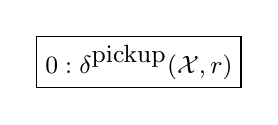
\begin{tikzpicture}
\small
\matrix[nodes={minimum size=6mm}] {
  \node[draw] {$0:\delta^\textrm{pickup}(\mathcal{X},r)$};\\
};
\end{tikzpicture}

where $r$ is the request identified by {\tt{}rid} (param. 1).\\
\textbf{Side Effects:} none.\\
\textbf{Throws:} {\tt{}SQLException} if database failure is encountered.\\
\bottomrule
\end{tabular}
\nwenddocs{}\nwbegincode{53}\sublabel{NW18ZcDF-3eqIl6-1}\nwmargintag{{\nwtagstyle{}\subpageref{NW18ZcDF-3eqIl6-1}}}\moddef{Read: DBQueryRequestDurationPickup(1)~{\nwtagstyle{}\subpageref{NW18ZcDF-3eqIl6-1}}}\endmoddef\nwused{\\{NW3x1zuR-Oyob-1}}
int[] DBQueryRequestDurationPickup(final int rid) throws SQLException \{
  try (\LA{}Open \code{}conn\edoc{}~{\nwtagstyle{}\subpageref{NWgUSr6-JT1v9-1}}\RA{}) \{
    return PSQuery(conn, "S118", 1, rid);
  \} catch (SQLException e) \{
    throw e;
  \}
\}
\nwindexdefn{DBQueryRequestDurationPickup}{DBQueryRequestDurationPickup}{NW18ZcDF-3eqIl6-1}\eatline
\nwidentdefs{\\{{DBQueryRequestDurationPickup}{DBQueryRequestDurationPickup}}}\nwidentuses{\\{{PSQuery}{PSQuery}}\\{{S118}{S118}}}\nwindexuse{PSQuery}{PSQuery}{NW18ZcDF-3eqIl6-1}\nwindexuse{S118}{S118}{NW18ZcDF-3eqIl6-1}\nwendcode{}\nwbegindocs{54}\nwdocspar
\subsection{\texttt{DBQueryRequestDurationTransit}(1)}
\begin{tabular}{p{\textwidth}}
\toprule
\rowcolor{TableTitle}
Method \textcolor{blue}{{\tt{}\protect\nwindexuse{DBQueryRequestDurationTransit}{DBQueryRequestDurationTransit}{NW18ZcDF-4Aq6dV-1}DBQueryRequestDurationTransit}}(1) returns the
transit duration $\delta^\textrm{transit}(\mathcal{X},r)$
(Eq.~\ref{eq:transit-duration}) of the given request.
A {\tt{}SQLException} is thrown in case of database failure.\\
\midrule
\textbf{Parameters:}\\
\begin{tabular}{lp{116mm}}
Integer {\tt{}rid} (param. 1):&request identifier.
\end{tabular}\\
\textbf{Returns:} results of the query flattened into an integer array,
or {\tt{}null} if no results.

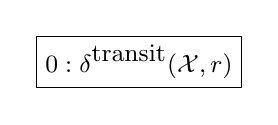
\begin{tikzpicture}
\small
\matrix[nodes={minimum size=6mm}] {
  \node[draw] {$0:\delta^\textrm{transit}(\mathcal{X},r)$};\\
};
\end{tikzpicture}

where $r$ is the request identified by {\tt{}rid} (param. 1).\\
\textbf{Side Effects:} none.\\
\textbf{Throws:} {\tt{}SQLException} if database failure is encountered.\\
\bottomrule
\end{tabular}
\nwenddocs{}\nwbegincode{55}\sublabel{NW18ZcDF-4Aq6dV-1}\nwmargintag{{\nwtagstyle{}\subpageref{NW18ZcDF-4Aq6dV-1}}}\moddef{Read: DBQueryRequestDurationTransit(1)~{\nwtagstyle{}\subpageref{NW18ZcDF-4Aq6dV-1}}}\endmoddef\nwused{\\{NW3x1zuR-Oyob-1}}
int[] DBQueryRequestDurationTransit(final int rid) throws SQLException \{
  try (\LA{}Open \code{}conn\edoc{}~{\nwtagstyle{}\subpageref{NWgUSr6-JT1v9-1}}\RA{}) \{
    return PSQuery(conn, "S120", 1, rid);
  \} catch (SQLException e) \{
    throw e;
  \}
\}
\nwindexdefn{DBQueryRequestDurationTransit}{DBQueryRequestDurationTransit}{NW18ZcDF-4Aq6dV-1}\eatline
\nwidentdefs{\\{{DBQueryRequestDurationTransit}{DBQueryRequestDurationTransit}}}\nwidentuses{\\{{PSQuery}{PSQuery}}\\{{S120}{S120}}}\nwindexuse{PSQuery}{PSQuery}{NW18ZcDF-4Aq6dV-1}\nwindexuse{S120}{S120}{NW18ZcDF-4Aq6dV-1}\nwendcode{}\nwbegindocs{56}\nwdocspar
\subsection{\texttt{DBQueryRequestDurationTravel}(1)}
\begin{tabular}{p{\textwidth}}
\toprule
\rowcolor{TableTitle}
Method \textcolor{blue}{{\tt{}\protect\nwindexuse{DBQueryRequestDurationTravel}{DBQueryRequestDurationTravel}{NW18ZcDF-3CyHZy-1}DBQueryRequestDurationTravel}}(1) returns the
travel duration $\delta^\textrm{travel}(\mathcal{X},r)$
(Eq.~\ref{eq:travel-duration}) of the given request.
A {\tt{}SQLException} is thrown in case of database failure.\\
\midrule
\textbf{Parameters:}\\
\begin{tabular}{lp{116mm}}
Integer {\tt{}rid} (param. 1):&request identifier.
\end{tabular}\\
\textbf{Returns:} results of the query flattened into an integer array,
or {\tt{}null} if no results.

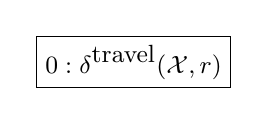
\begin{tikzpicture}
\small
\matrix[nodes={minimum size=6mm}] {
  \node[draw] {$0:\delta^\textrm{travel}(\mathcal{X},r)$};\\
};
\end{tikzpicture}

where $r$ is the request identified by {\tt{}rid} (param. 1).\\
\textbf{Side Effects:} none.\\
\textbf{Throws:} {\tt{}SQLException} if database failure is encountered.\\
\bottomrule
\end{tabular}
\nwenddocs{}\nwbegincode{57}\sublabel{NW18ZcDF-3CyHZy-1}\nwmargintag{{\nwtagstyle{}\subpageref{NW18ZcDF-3CyHZy-1}}}\moddef{Read: DBQueryRequestDurationTravel(1)~{\nwtagstyle{}\subpageref{NW18ZcDF-3CyHZy-1}}}\endmoddef\nwused{\\{NW3x1zuR-Oyob-1}}
int[] DBQueryRequestDurationTravel(final int rid) throws SQLException \{
  try (\LA{}Open \code{}conn\edoc{}~{\nwtagstyle{}\subpageref{NWgUSr6-JT1v9-1}}\RA{}) \{
    return PSQuery(conn, "S122", 1, rid);
  \} catch (SQLException e) \{
    throw e;
  \}
\}
\nwindexdefn{DBQueryRequestDurationTravel}{DBQueryRequestDurationTravel}{NW18ZcDF-3CyHZy-1}\eatline
\nwidentdefs{\\{{DBQueryRequestDurationTravel}{DBQueryRequestDurationTravel}}}\nwidentuses{\\{{PSQuery}{PSQuery}}\\{{S122}{S122}}}\nwindexuse{PSQuery}{PSQuery}{NW18ZcDF-3CyHZy-1}\nwindexuse{S122}{S122}{NW18ZcDF-3CyHZy-1}\nwendcode{}\nwbegindocs{58}\nwdocspar
\subsection{\texttt{DBQueryRequestTimeOfDeparture}(1)}
\begin{tabular}{p{\textwidth}}
\toprule
\rowcolor{TableTitle}
Method \textcolor{blue}{{\tt{}\protect\nwindexuse{DBQueryRequestTimeOfDeparture}{DBQueryRequestTimeOfDeparture}{NW18ZcDF-dlG5g-1}DBQueryRequestTimeOfDeparture}}(1) returns the
departure time $t^\textrm{depart}(\mathcal{X},r)$
(Eq.~\ref{eq:departure-time}) of the given request.
A {\tt{}SQLException} is thrown in case of database failure.\\
\midrule
\textbf{Parameters:}\\
\begin{tabular}{lp{116mm}}
Integer {\tt{}rid} (param. 1):&request identifier.
\end{tabular}\\
\textbf{Returns:} results of the query flattened into an integer array,
or {\tt{}null} if no results.

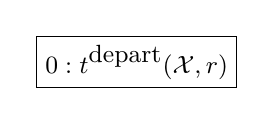
\begin{tikzpicture}
\small
\matrix[nodes={minimum size=6mm}] {
  \node[draw] {$0:t^\textrm{depart}(\mathcal{X},r)$};\\
};
\end{tikzpicture}

where $r$ is the request identified by {\tt{}rid} (param. 1).\\
\textbf{Side Effects:} none.\\
\textbf{Throws:} {\tt{}SQLException} if database failure is encountered.\\
\bottomrule
\end{tabular}
\nwenddocs{}\nwbegincode{59}\sublabel{NW18ZcDF-dlG5g-1}\nwmargintag{{\nwtagstyle{}\subpageref{NW18ZcDF-dlG5g-1}}}\moddef{Read: DBQueryRequestTimeOfDeparture(1)~{\nwtagstyle{}\subpageref{NW18ZcDF-dlG5g-1}}}\endmoddef\nwused{\\{NW3x1zuR-Oyob-1}}
int[] DBQueryRequestTimeOfDeparture(final int rid) throws SQLException \{
  try (\LA{}Open \code{}conn\edoc{}~{\nwtagstyle{}\subpageref{NWgUSr6-JT1v9-1}}\RA{}) \{
    return PSQuery(conn, "S124", 1, rid);
  \} catch (SQLException e) \{
    throw e;
  \}
\}
\nwindexdefn{DBQueryRequestTimeOfDeparture}{DBQueryRequestTimeOfDeparture}{NW18ZcDF-dlG5g-1}\eatline
\nwidentdefs{\\{{DBQueryRequestTimeOfDeparture}{DBQueryRequestTimeOfDeparture}}}\nwidentuses{\\{{PSQuery}{PSQuery}}\\{{S124}{S124}}}\nwindexuse{PSQuery}{PSQuery}{NW18ZcDF-dlG5g-1}\nwindexuse{S124}{S124}{NW18ZcDF-dlG5g-1}\nwendcode{}\nwbegindocs{60}\begin{tabular}{p{\textwidth}}
\toprule
\rowcolor{TableTitle}
Method \textcolor{blue}{{\tt{}\protect\nwindexuse{queryRequestTimeOfDeparture}{queryRequestTimeOfDeparture}{NW18ZcDF-JMT2Q-1}queryRequestTimeOfDeparture}}(1) wraps {\tt{}\protect\nwindexuse{DBQueryRequestTimeOfDeparture}{DBQueryRequestTimeOfDeparture}{NW18ZcDF-dlG5g-1}DBQueryRequestTimeOfDeparture}(1).\\
\bottomrule
\end{tabular}
\nwenddocs{}\nwbegincode{61}\sublabel{NW18ZcDF-JMT2Q-1}\nwmargintag{{\nwtagstyle{}\subpageref{NW18ZcDF-JMT2Q-1}}}\moddef{Read: queryRequestTimeOfDeparture(1)~{\nwtagstyle{}\subpageref{NW18ZcDF-JMT2Q-1}}}\endmoddef\nwused{\\{NW3x1zuR-2u8vSA-1}}
int[] queryRequestTimeOfDeparture(final int rid) throws SQLException \{
  return storage.DBQueryRequestTimeOfDeparture(rid);
\}
\nwindexdefn{queryRequestTimeOfDeparture}{queryRequestTimeOfDeparture}{NW18ZcDF-JMT2Q-1}\eatline
\nwidentdefs{\\{{queryRequestTimeOfDeparture}{queryRequestTimeOfDeparture}}}\nwidentuses{\\{{DBQueryRequestTimeOfDeparture}{DBQueryRequestTimeOfDeparture}}}\nwindexuse{DBQueryRequestTimeOfDeparture}{DBQueryRequestTimeOfDeparture}{NW18ZcDF-JMT2Q-1}\nwendcode{}\nwbegindocs{62}\nwdocspar
\subsection{\texttt{DBQueryRequestTimeOfArrival}(1)}
\begin{tabular}{p{\textwidth}}
\toprule
\rowcolor{TableTitle}
Method \textcolor{blue}{{\tt{}\protect\nwindexuse{DBQueryRequestTimeOfArrival}{DBQueryRequestTimeOfArrival}{NW18ZcDF-cz5yf-1}DBQueryRequestTimeOfArrival}}(1) returns the
arrival time $t^\textrm{arrive}(\mathcal{X},r)$
(Eq.~\ref{eq:arrival-time}) of the given request.
A {\tt{}SQLException} is thrown in case of database failure.\\
\midrule
\textbf{Parameters:}\\
\begin{tabular}{lp{116mm}}
Integer {\tt{}rid} (param. 1):&request identifier.
\end{tabular}\\
\textbf{Returns:} results of the query flattened into an integer array,
or {\tt{}null} if no results.

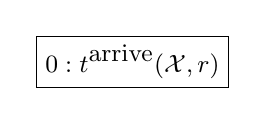
\begin{tikzpicture}
\small
\matrix[nodes={minimum size=6mm}] {
  \node[draw] {$0:t^\textrm{arrive}(\mathcal{X},r)$};\\
};
\end{tikzpicture}

where $r$ is the request identified by {\tt{}rid} (param. 1).\\
\textbf{Side Effects:} none.\\
\textbf{Throws:} {\tt{}SQLException} if database failure is encountered.\\
\bottomrule
\end{tabular}
\nwenddocs{}\nwbegincode{63}\sublabel{NW18ZcDF-cz5yf-1}\nwmargintag{{\nwtagstyle{}\subpageref{NW18ZcDF-cz5yf-1}}}\moddef{Read: DBQueryRequestTimeOfArrival(1)~{\nwtagstyle{}\subpageref{NW18ZcDF-cz5yf-1}}}\endmoddef\nwused{\\{NW3x1zuR-Oyob-1}}
int[] DBQueryRequestTimeOfArrival(final int rid) throws SQLException \{
  try (\LA{}Open \code{}conn\edoc{}~{\nwtagstyle{}\subpageref{NWgUSr6-JT1v9-1}}\RA{}) \{
    return PSQuery(conn, "S126", 1, rid);
  \} catch (SQLException e) \{
    throw e;
  \}
\}
\nwindexdefn{DBQueryRequestTimeOfArrival}{DBQueryRequestTimeOfArrival}{NW18ZcDF-cz5yf-1}\eatline
\nwidentdefs{\\{{DBQueryRequestTimeOfArrival}{DBQueryRequestTimeOfArrival}}}\nwidentuses{\\{{PSQuery}{PSQuery}}\\{{S126}{S126}}}\nwindexuse{PSQuery}{PSQuery}{NW18ZcDF-cz5yf-1}\nwindexuse{S126}{S126}{NW18ZcDF-cz5yf-1}\nwendcode{}\nwbegindocs{64}\begin{tabular}{p{\textwidth}}
\toprule
\rowcolor{TableTitle}
Method \textcolor{blue}{{\tt{}\protect\nwindexuse{queryRequestTimeOfArrival}{queryRequestTimeOfArrival}{NW18ZcDF-2DgZiX-1}queryRequestTimeOfArrival}}(1) wraps {\tt{}\protect\nwindexuse{DBQueryRequestTimeOfArrival}{DBQueryRequestTimeOfArrival}{NW18ZcDF-cz5yf-1}DBQueryRequestTimeOfArrival}(1).\\
\bottomrule
\end{tabular}
\nwenddocs{}\nwbegincode{65}\sublabel{NW18ZcDF-2DgZiX-1}\nwmargintag{{\nwtagstyle{}\subpageref{NW18ZcDF-2DgZiX-1}}}\moddef{Read: queryRequestTimeOfArrival(1)~{\nwtagstyle{}\subpageref{NW18ZcDF-2DgZiX-1}}}\endmoddef\nwused{\\{NW3x1zuR-2u8vSA-1}}
int[] queryRequestTimeOfArrival(final int rid) throws SQLException \{
  return storage.DBQueryRequestTimeOfArrival(rid);
\}
\nwindexdefn{queryRequestTimeOfArrival}{queryRequestTimeOfArrival}{NW18ZcDF-2DgZiX-1}\eatline
\nwidentdefs{\\{{queryRequestTimeOfArrival}{queryRequestTimeOfArrival}}}\nwidentuses{\\{{DBQueryRequestTimeOfArrival}{DBQueryRequestTimeOfArrival}}}\nwindexuse{DBQueryRequestTimeOfArrival}{DBQueryRequestTimeOfArrival}{NW18ZcDF-2DgZiX-1}\nwendcode{}\nwbegindocs{66}\nwdocspar
\subsection{\texttt{DBQueryRequestsCount}(0)}
\begin{tabular}{p{\textwidth}}
\toprule
\rowcolor{TableTitle}
Method \textcolor{blue}{{\tt{}\protect\nwindexuse{DBQueryRequestsCount}{DBQueryRequestsCount}{NW18ZcDF-3PzevO-1}DBQueryRequestsCount}}(0) returns the total number
of requests in Table R.
A {\tt{}SQLException} is thrown in case of database failure.\\
\midrule
\textbf{Parameters:} none.\\
\textbf{Returns:} results of the query flattened into an integer array, or
{\tt{}null} if no results.

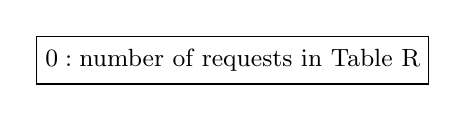
\begin{tikzpicture}
\small
\matrix[nodes={draw,minimum size=6mm}] {
  \node {$0:\textrm{number of requests in Table R}$};\\
};
\end{tikzpicture}\\
\textbf{Side Effects:} none.\\
\textbf{Throws:} {\tt{}SQLException} if database failure is encountered.\\
\bottomrule
\end{tabular}
\nwenddocs{}\nwbegincode{67}\sublabel{NW18ZcDF-3PzevO-1}\nwmargintag{{\nwtagstyle{}\subpageref{NW18ZcDF-3PzevO-1}}}\moddef{Read: DBQueryRequestsCount(0)~{\nwtagstyle{}\subpageref{NW18ZcDF-3PzevO-1}}}\endmoddef\nwused{\\{NW3x1zuR-Oyob-1}}
int[] DBQueryRequestsCount() throws SQLException \{
  try (\LA{}Open \code{}conn\edoc{}~{\nwtagstyle{}\subpageref{NWgUSr6-JT1v9-1}}\RA{}) \{
    return this.PSQuery(conn, "S67", 1);
  \} catch (SQLException e) \{
    throw e;
  \}
\}
\nwindexdefn{DBQueryRequestsCount}{DBQueryRequestsCount}{NW18ZcDF-3PzevO-1}\eatline
\nwidentdefs{\\{{DBQueryRequestsCount}{DBQueryRequestsCount}}}\nwidentuses{\\{{PSQuery}{PSQuery}}\\{{S67}{S67}}}\nwindexuse{PSQuery}{PSQuery}{NW18ZcDF-3PzevO-1}\nwindexuse{S67}{S67}{NW18ZcDF-3PzevO-1}\nwendcode{}\nwbegindocs{68}\begin{tabular}{p{\textwidth}}
\toprule
\rowcolor{TableTitle}
Method \textcolor{blue}{{\tt{}\protect\nwindexuse{queryRequestsCount}{queryRequestsCount}{NW18ZcDF-4WSGXN-1}queryRequestsCount}}(0) wraps {\tt{}\protect\nwindexuse{DBQueryRequestsCount}{DBQueryRequestsCount}{NW18ZcDF-3PzevO-1}DBQueryRequestsCount}(0).\\
\bottomrule
\end{tabular}
\nwenddocs{}\nwbegincode{69}\sublabel{NW18ZcDF-4WSGXN-1}\nwmargintag{{\nwtagstyle{}\subpageref{NW18ZcDF-4WSGXN-1}}}\moddef{Read: queryRequestsCount(0)~{\nwtagstyle{}\subpageref{NW18ZcDF-4WSGXN-1}}}\endmoddef\nwused{\\{NW3x1zuR-2u8vSA-1}}
int[] queryRequestsCount() throws SQLException \{
  return storage.DBQueryRequestsCount();
\}
\nwindexdefn{queryRequestsCount}{queryRequestsCount}{NW18ZcDF-4WSGXN-1}\eatline
\nwidentdefs{\\{{queryRequestsCount}{queryRequestsCount}}}\nwidentuses{\\{{DBQueryRequestsCount}{DBQueryRequestsCount}}}\nwindexuse{DBQueryRequestsCount}{DBQueryRequestsCount}{NW18ZcDF-4WSGXN-1}\nwendcode{}\nwbegindocs{70}\nwdocspar
\subsection{\texttt{DBQueryRequestsQueued}(1)}
\begin{tabular}{p{\textwidth}}
\toprule
\rowcolor{TableTitle}
Method \textcolor{blue}{{\tt{}\protect\nwindexuse{DBQueryRequestsQueued}{DBQueryRequestsQueued}{NW18ZcDF-4AIMTx-1}DBQueryRequestsQueued}}(1) returns the requests
eligible for assignment at the given time. A request $r$ is ``eligible'' if it
is not assigned at the given time, and if the given time is between the
request's early time $r_\texttt{e}$ and
$(r_\texttt{e}+\texttt{REQUEST\_TIMEOUT})$.
A {\tt{}SQLException} is thrown in case of database failure.\\
\midrule
\textbf{Parameters:} \\
\begin{tabular}{lp{116mm}}
Integer {\tt{}t} (param. 1):&a time
\end{tabular}\\
\textbf{Returns:} results of the query flattened into an integer array, or
{\tt{}null} if no results.

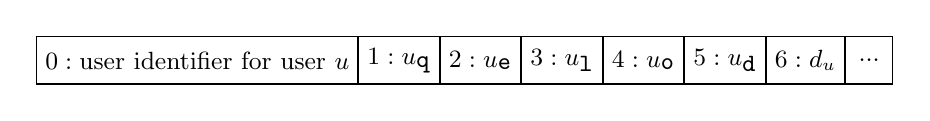
\begin{tikzpicture}
\small
\matrix[nodes={draw,minimum size=6mm}] {
  \node {$0:\textrm{user identifier for user $u$}$};
 &\node {$1:u_\texttt{q}$};
 &\node {$2:u_\texttt{e}$};
 &\node {$3:u_\texttt{l}$};
 &\node {$4:u_\texttt{o}$};
 &\node {$5:u_\texttt{d}$};
 &\node {$6:d_u$};
 &\node {...};\\
};
\end{tikzpicture}\\
\textbf{Side Effects:} none.\\
\textbf{Throws:} {\tt{}SQLException} if database failure is encountered.\\
\bottomrule
\end{tabular}
\nwenddocs{}\nwbegincode{71}\sublabel{NW18ZcDF-4AIMTx-1}\nwmargintag{{\nwtagstyle{}\subpageref{NW18ZcDF-4AIMTx-1}}}\moddef{Read: DBQueryRequestsQueued(1)~{\nwtagstyle{}\subpageref{NW18ZcDF-4AIMTx-1}}}\endmoddef\nwalsodefined{\\{NW18ZcDF-4AIMTx-2}\\{NW18ZcDF-4AIMTx-3}}\nwused{\\{NW3x1zuR-Oyob-1}}
int[] DBQueryRequestsQueued(final int t) throws SQLException \{
  try (\LA{}Open \code{}conn\edoc{}~{\nwtagstyle{}\subpageref{NWgUSr6-JT1v9-1}}\RA{}) \{
\nosublabel{NW18ZcDF-4AIMTx-1-u1}\nwindexdefn{DBQueryRequestsQueued}{DBQueryRequestsQueued}{NW18ZcDF-4AIMTx-1}\eatline
\nwidentdefs{\\{{DBQueryRequestsQueued}{DBQueryRequestsQueued}}}\nwendcode{}\nwbegindocs{72}{\small Our approach is to first select all requests where $t$ is between the
request's early time $r_\texttt{e}$ and
$r_\texttt{e}+\texttt{REQUEST\_TIMEOUT}$.  Then, we return a filtered subset of
these requests that are unassigned. As we don't know how many requests will
returned in the end, we initialize a temporary array {\tt{}temp1} to hold the
pre-filter number of requests.}
\nwenddocs{}\nwbegincode{73}\sublabel{NW18ZcDF-4AIMTx-2}\nwmargintag{{\nwtagstyle{}\subpageref{NW18ZcDF-4AIMTx-2}}}\moddef{Read: DBQueryRequestsQueued(1)~{\nwtagstyle{}\subpageref{NW18ZcDF-4AIMTx-1}}}\plusendmoddef
    final int[] output = this.PSQuery(conn, "S143", 7, t, t, REQUEST_TIMEOUT);
    int[] temp1 = new int[output.length];
    int j = 0;
    for (int i = 0; i < (output.length - 6); i += 7) \{
      if (this.lu_rstatus.get(output[i]) == false) \{
        temp1[(j + 0)] = output[(i + 0)];
        temp1[(j + 1)] = output[(i + 1)];
        temp1[(j + 2)] = output[(i + 2)];
        temp1[(j + 3)] = output[(i + 3)];
        temp1[(j + 4)] = output[(i + 4)];
        temp1[(j + 5)] = output[(i + 5)];
        temp1[(j + 6)] = output[(i + 6)];
        j += 7;
      \}
    \}
\nwidentuses{\\{{PSQuery}{PSQuery}}\\{{S143}{S143}}}\nwindexuse{PSQuery}{PSQuery}{NW18ZcDF-4AIMTx-2}\nwindexuse{S143}{S143}{NW18ZcDF-4AIMTx-2}\nwendcode{}\nwbegindocs{74}\nwdocspar
\nwenddocs{}\nwbegincode{75}\sublabel{NW18ZcDF-4AIMTx-3}\nwmargintag{{\nwtagstyle{}\subpageref{NW18ZcDF-4AIMTx-3}}}\moddef{Read: DBQueryRequestsQueued(1)~{\nwtagstyle{}\subpageref{NW18ZcDF-4AIMTx-1}}}\plusendmoddef
    return Arrays.copyOf(temp1, j);
  \} catch (SQLException e) \{
    throw e;
  \}
\}
\nwendcode{}\nwbegindocs{76}\nwdocspar
\begin{tabular}{p{\textwidth}}
\toprule
\rowcolor{TableTitle}
Method \textcolor{blue}{{\tt{}\protect\nwindexuse{queryRequestsQueued}{queryRequestsQueued}{NW18ZcDF-2FYATt-1}queryRequestsQueued}}(1) wraps {\tt{}\protect\nwindexuse{DBQueryRequestsQueued}{DBQueryRequestsQueued}{NW18ZcDF-4AIMTx-1}DBQueryRequestsQueued}(1).\\
\bottomrule
\end{tabular}
\nwenddocs{}\nwbegincode{77}\sublabel{NW18ZcDF-2FYATt-1}\nwmargintag{{\nwtagstyle{}\subpageref{NW18ZcDF-2FYATt-1}}}\moddef{Read: queryRequestsQueued(1)~{\nwtagstyle{}\subpageref{NW18ZcDF-2FYATt-1}}}\endmoddef\nwused{\\{NW3x1zuR-2u8vSA-1}}
int[] queryRequestsQueued(final int t) throws SQLException \{
  return storage.DBQueryRequestsQueued(t);
\}
\nwindexdefn{queryRequestsQueued}{queryRequestsQueued}{NW18ZcDF-2FYATt-1}\eatline
\nwidentdefs{\\{{queryRequestsQueued}{queryRequestsQueued}}}\nwidentuses{\\{{DBQueryRequestsQueued}{DBQueryRequestsQueued}}}\nwindexuse{DBQueryRequestsQueued}{DBQueryRequestsQueued}{NW18ZcDF-2FYATt-1}\nwendcode{}\nwbegindocs{78}\nwdocspar
\subsection{\texttt{DBQueryServerRoute}(1)}
\begin{tabular}{p{\textwidth}}
\toprule
\rowcolor{TableTitle}
Method \textcolor{blue}{{\tt{}\protect\nwindexuse{DBQueryServerRoute}{DBQueryServerRoute}{NW18ZcDF-1cB9Z1-1}DBQueryServerRoute}}(1) returns the route for the
given server identified by {\tt{}sid} (param. 1) at time $t$ (param. 2).
A {\tt{}SQLException} is thrown in case of database failure.\\
\midrule
\textbf{Parameters:} \\
\begin{tabular}{lp{116mm}}
Integer {\tt{}sid} (param. 1):&server identifier.\\
\end{tabular}
\textbf{Returns:} results of the query flattened into an integer array,
or {\tt{}null} if no results.

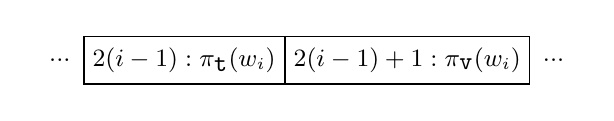
\begin{tikzpicture}
\small
\matrix[nodes={minimum size=6mm}] {
  \node {...};
 &\node[draw] {$2(i-1):\pi_\texttt{t}(w_i)$};
 &\node[draw] {$2(i-1)+1:\pi_\texttt{v}(w_i)$};
 &\node {...};\\
};
\end{tikzpicture}

where $1\leq i\leq |w|$ and $w$ is the route for the given server
identified by {\tt{}sid} (param. 1).\\
\textbf{Side Effects:} none.\\
\textbf{Throws:} {\tt{}SQLException} if database failure is encountered.\\
\bottomrule
\end{tabular}
\nwenddocs{}\nwbegincode{79}\sublabel{NW18ZcDF-1cB9Z1-1}\nwmargintag{{\nwtagstyle{}\subpageref{NW18ZcDF-1cB9Z1-1}}}\moddef{Read: DBQueryServerRoute(1)~{\nwtagstyle{}\subpageref{NW18ZcDF-1cB9Z1-1}}}\endmoddef\nwused{\\{NW3x1zuR-Oyob-1}}
int[] DBQueryServerRoute(final int sid) throws SQLException \{
  try (\LA{}Open \code{}conn\edoc{}~{\nwtagstyle{}\subpageref{NWgUSr6-JT1v9-1}}\RA{}) \{
    return PSQuery(conn, "S60", 2, sid);
  \} catch (SQLException e) \{
    throw e;
  \}
\}
\nwindexdefn{DBQueryServerRoute}{DBQueryServerRoute}{NW18ZcDF-1cB9Z1-1}\eatline
\nwidentdefs{\\{{DBQueryServerRoute}{DBQueryServerRoute}}}\nwidentuses{\\{{PSQuery}{PSQuery}}\\{{S60}{S60}}}\nwindexuse{PSQuery}{PSQuery}{NW18ZcDF-1cB9Z1-1}\nwindexuse{S60}{S60}{NW18ZcDF-1cB9Z1-1}\nwendcode{}\nwbegindocs{80}\begin{tabular}{p{\textwidth}}
\toprule
\rowcolor{TableTitle}
Method \textcolor{blue}{{\tt{}\protect\nwindexuse{queryServerRoute}{queryServerRoute}{NW18ZcDF-3INKD2-1}queryServerRoute}}(1) wraps {\tt{}\protect\nwindexuse{DBQueryServerRoute}{DBQueryServerRoute}{NW18ZcDF-1cB9Z1-1}DBQueryServerRoute}(1).\\
\bottomrule
\end{tabular}
\nwenddocs{}\nwbegincode{81}\sublabel{NW18ZcDF-3INKD2-1}\nwmargintag{{\nwtagstyle{}\subpageref{NW18ZcDF-3INKD2-1}}}\moddef{Read: queryServerRoute(1)~{\nwtagstyle{}\subpageref{NW18ZcDF-3INKD2-1}}}\endmoddef\nwused{\\{NW3x1zuR-2u8vSA-1}}
int[] queryServerRoute(final int sid) throws SQLException \{
  return storage.DBQueryServerRoute(sid);
\}
\nwindexdefn{queryServerRoute}{queryServerRoute}{NW18ZcDF-3INKD2-1}\eatline
\nwidentdefs{\\{{queryServerRoute}{queryServerRoute}}}\nwidentuses{\\{{DBQueryServerRoute}{DBQueryServerRoute}}}\nwindexuse{DBQueryServerRoute}{DBQueryServerRoute}{NW18ZcDF-3INKD2-1}\nwendcode{}\nwbegindocs{82}\nwdocspar
\subsection{\texttt{DBQueryServerRouteRemaining}(2)}
\begin{tabular}{p{\textwidth}}
\toprule
\rowcolor{TableTitle}
Method \textcolor{blue}{{\tt{}\protect\nwindexuse{DBQueryServerRouteRemaining}{DBQueryServerRouteRemaining}{NW18ZcDF-4JTjfI-1}DBQueryServerRouteRemaining}}(2) returns the
remaining route for the given server at the given time.
A {\tt{}SQLException} is thrown in case of database failure.\\
\midrule
\textbf{Parameters:} \\
\begin{tabular}{lp{116mm}}
Integer {\tt{}sid} (param. 1):&server identifier.\\
Integer {\tt{}t} (param. 2):&a time.\\
\end{tabular}
\textbf{Returns:} results of the query flattened into an integer array,
or {\tt{}null} if no results.

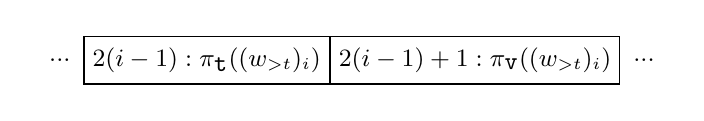
\begin{tikzpicture}
\small
\matrix[nodes={minimum size=6mm}] {
  \node {...};
 &\node[draw] {$2(i-1):\pi_\texttt{t}({(w_{>t}})_i)$};
 &\node[draw] {$2(i-1)+1:\pi_\texttt{v}({(w_{>t}})_i)$};
 &\node {...};\\
};
\end{tikzpicture}

where $1\leq i\leq |w_{>t}|$ and $w_{>t}$ is the remaining route for the
given server identified by {\tt{}sid} (param. 1) at time $t$ (param. 2).\\
\textbf{Side Effects:} none.\\
\textbf{Throws:} {\tt{}SQLException} if database failure is encountered.\\
\bottomrule
\end{tabular}
\nwenddocs{}\nwbegincode{83}\sublabel{NW18ZcDF-4JTjfI-1}\nwmargintag{{\nwtagstyle{}\subpageref{NW18ZcDF-4JTjfI-1}}}\moddef{Read: DBQueryServerRouteRemaining(2)~{\nwtagstyle{}\subpageref{NW18ZcDF-4JTjfI-1}}}\endmoddef\nwused{\\{NW3x1zuR-Oyob-1}}
int[] DBQueryServerRouteRemaining(final int sid, final int t) throws SQLException \{
  try (\LA{}Open \code{}conn\edoc{}~{\nwtagstyle{}\subpageref{NWgUSr6-JT1v9-1}}\RA{}) \{
    return PSQuery(conn, "S129", 2, sid, t);
  \} catch (SQLException e) \{
    throw e;
  \}
\}
\nwindexdefn{DBQueryServerRouteRemaining}{DBQueryServerRouteRemaining}{NW18ZcDF-4JTjfI-1}\eatline
\nwidentdefs{\\{{DBQueryServerRouteRemaining}{DBQueryServerRouteRemaining}}}\nwidentuses{\\{{PSQuery}{PSQuery}}\\{{S129}{S129}}}\nwindexuse{PSQuery}{PSQuery}{NW18ZcDF-4JTjfI-1}\nwindexuse{S129}{S129}{NW18ZcDF-4JTjfI-1}\nwendcode{}\nwbegindocs{84}\begin{tabular}{p{\textwidth}}
\toprule
\rowcolor{TableTitle}
Method \textcolor{blue}{{\tt{}\protect\nwindexuse{queryServerRouteRemaining}{queryServerRouteRemaining}{NW18ZcDF-3EQWyS-1}queryServerRouteRemaining}}(2) wraps {\tt{}\protect\nwindexuse{DBQueryServerRouteRemaining}{DBQueryServerRouteRemaining}{NW18ZcDF-4JTjfI-1}DBQueryServerRouteRemaining}(2).\\
\bottomrule
\end{tabular}
\nwenddocs{}\nwbegincode{85}\sublabel{NW18ZcDF-3EQWyS-1}\nwmargintag{{\nwtagstyle{}\subpageref{NW18ZcDF-3EQWyS-1}}}\moddef{Read: queryServerRouteRemaining(2)~{\nwtagstyle{}\subpageref{NW18ZcDF-3EQWyS-1}}}\endmoddef\nwused{\\{NW3x1zuR-2Rlctf-1}}
int[] queryServerRouteRemaining(final int sid, final int t) throws SQLException \{
  long A0 = System.currentTimeMillis();
  int[] output = this.storage.DBQueryServerRouteRemaining(sid, t);
  \LA{}Stats: queryServerRouteRemaining~{\nwtagstyle{}\subpageref{NW1n2CZQ-2Gmc1g-1}}\RA{}
  return output;
\}
\nosublabel{NW18ZcDF-3EQWyS-1-u1}\nwindexdefn{queryServerRouteRemaining}{queryServerRouteRemaining}{NW18ZcDF-3EQWyS-1}\eatline
\nwidentdefs{\\{{queryServerRouteRemaining}{queryServerRouteRemaining}}}\nwidentuses{\\{{DBQueryServerRouteRemaining}{DBQueryServerRouteRemaining}}}\nwindexuse{DBQueryServerRouteRemaining}{DBQueryServerRouteRemaining}{NW18ZcDF-3EQWyS-1}\nwendcode{}\nwbegindocs{86}\nwdocspar
\subsection{\texttt{DBQueryServerSchedule}(1)}
\begin{tabular}{p{\textwidth}}
\toprule
\rowcolor{TableTitle}
Method \textcolor{blue}{{\tt{}\protect\nwindexuse{DBQueryServerSchedule}{DBQueryServerSchedule}{NW18ZcDF-71ppP-1}DBQueryServerSchedule}}(1) returns the schedule
for the given server.
A {\tt{}SQLException} is thrown in case of database failure.\\
\midrule
\textbf{Parameters:} \\
\begin{tabular}{lp{116mm}}
Integer {\tt{}sid} (param. 1):&server identifier.\\
\end{tabular}
\textbf{Returns:} results of the query flattened into an integer array,
or {\tt{}null} if no results.

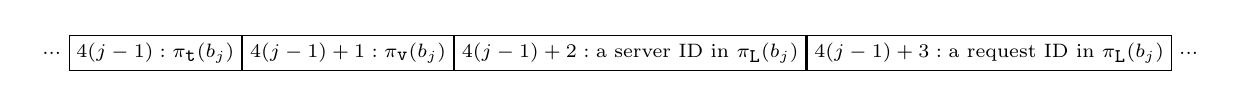
\begin{tikzpicture}
\scriptsize
\matrix[nodes={}] {
  \node {...};
 &\node[draw] {$4(j-1):\pi_\texttt{t}(b_j)$};
 &\node[draw] {$4(j-1)+1:\pi_\texttt{v}(b_j)$};
 &\node[draw] {$4(j-1)+2:\textrm{a server ID in }\pi_\texttt{L}(b_j)$};
 &\node[draw] {$4(j-1)+3:\textrm{a request ID in }\pi_\texttt{L}(b_j)$};
 &\node {...};\\
};
\end{tikzpicture}

where $1\leq j\leq |b|$ and $b$ is the schedule for the
given server  identified by {\tt{}sid} (param. 1).
If a label is empty (\textit{e.g.} not all waypoints will have a server
identifier in their label set), the element will be 0. If a waypoint has
multiple labels, the waypoint will be written once for each of the labels.
The returned sequence is in time-ascending order but \textbf{is not guaranteed}
to be in the same order as the actual pick-ups and drop-offs, \textit{e.g.} if a
waypoint has multiple labels with some indicating pick-ups and some indicating
drop-offs, the ordering of these waypoints is uncertain.\\
\textbf{Side Effects:} none.\\
\textbf{Throws:} {\tt{}SQLException} if database failure is encountered.\\
\bottomrule
\end{tabular}
\nwenddocs{}\nwbegincode{87}\sublabel{NW18ZcDF-71ppP-1}\nwmargintag{{\nwtagstyle{}\subpageref{NW18ZcDF-71ppP-1}}}\moddef{Read: DBQueryServerSchedule(1)~{\nwtagstyle{}\subpageref{NW18ZcDF-71ppP-1}}}\endmoddef\nwused{\\{NW3x1zuR-Oyob-1}}
int[] DBQueryServerSchedule(final int sid) throws SQLException \{
  try (\LA{}Open \code{}conn\edoc{}~{\nwtagstyle{}\subpageref{NWgUSr6-JT1v9-1}}\RA{}) \{
    return PSQuery(conn, "S61", 4, sid);
  \} catch (SQLException e) \{
    throw e;
  \}
\}
\nwindexdefn{DBQueryServerSchedule}{DBQueryServerSchedule}{NW18ZcDF-71ppP-1}\eatline
\nwidentdefs{\\{{DBQueryServerSchedule}{DBQueryServerSchedule}}}\nwidentuses{\\{{PSQuery}{PSQuery}}\\{{S61}{S61}}}\nwindexuse{PSQuery}{PSQuery}{NW18ZcDF-71ppP-1}\nwindexuse{S61}{S61}{NW18ZcDF-71ppP-1}\nwendcode{}\nwbegindocs{88}\begin{tabular}{p{\textwidth}}
\toprule
\rowcolor{TableTitle}
Method \textcolor{blue}{{\tt{}\protect\nwindexuse{queryServerSchedule}{queryServerSchedule}{NW18ZcDF-2vGK9z-1}queryServerSchedule}}(1) wraps {\tt{}\protect\nwindexuse{DBQueryServerSchedule}{DBQueryServerSchedule}{NW18ZcDF-71ppP-1}DBQueryServerSchedule}(1).\\
\bottomrule
\end{tabular}
\nwenddocs{}\nwbegincode{89}\sublabel{NW18ZcDF-2vGK9z-1}\nwmargintag{{\nwtagstyle{}\subpageref{NW18ZcDF-2vGK9z-1}}}\moddef{Read: queryServerSchedule(1)~{\nwtagstyle{}\subpageref{NW18ZcDF-2vGK9z-1}}}\endmoddef\nwused{\\{NW3x1zuR-2u8vSA-1}}
int[] queryServerSchedule(final int sid) throws SQLException \{
  return storage.DBQueryServerSchedule(sid);
\}
\nwindexdefn{queryServerSchedule}{queryServerSchedule}{NW18ZcDF-2vGK9z-1}\eatline
\nwidentdefs{\\{{queryServerSchedule}{queryServerSchedule}}}\nwidentuses{\\{{DBQueryServerSchedule}{DBQueryServerSchedule}}}\nwindexuse{DBQueryServerSchedule}{DBQueryServerSchedule}{NW18ZcDF-2vGK9z-1}\nwendcode{}\nwbegindocs{90}\nwdocspar
\subsection{\texttt{DBQueryServerScheduleRemaining}(2)}
\begin{tabular}{p{\textwidth}}
\toprule
\rowcolor{TableTitle}
Method \textcolor{blue}{{\tt{}\protect\nwindexuse{DBQueryServerScheduleRemaining}{DBQueryServerScheduleRemaining}{NW18ZcDF-48DsrJ-1}DBQueryServerScheduleRemaining}}(2) returns the
remaining schedule for the given server at the given time.
A {\tt{}SQLException} is thrown in case of database failure.\\
\midrule
\textbf{Parameters:} \\
\begin{tabular}{lp{116mm}}
Integer {\tt{}sid} (param. 1):&server identifier.\\
Integer {\tt{}t} (param. 2):&a time.\\
\end{tabular}
\textbf{Returns:} results of the query flattened into an integer array,
or {\tt{}null} if no results.

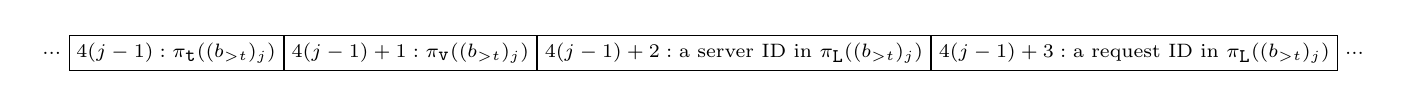
\begin{tikzpicture}
\scriptsize
\matrix[nodes={}] {
  \node {...};
 &\node[draw] {$4(j-1):\pi_\texttt{t}((b_{>t})_j)$};
 &\node[draw] {$4(j-1)+1:\pi_\texttt{v}((b_{>t})_j)$};
 &\node[draw] {$4(j-1)+2:\textrm{a server ID in }\pi_\texttt{L}((b_{>t})_j)$};
 &\node[draw] {$4(j-1)+3:\textrm{a request ID in }\pi_\texttt{L}((b_{>t})_j)$};
 &\node {...};\\
};
\end{tikzpicture}

where $1\leq j\leq |b_{>t}|$ and $b_{>t}$ is the remaining schedule for the
given server identified by {\tt{}sid} (param. 1) at time $t$ (param. 2).
If a label is empty (\textit{e.g.} not all waypoints will have a server
identifier in their label set), the element will be 0. If a waypoint has
multiple labels, the waypoint will be written once for each of the labels.
The returned sequence is in time-ascending order and \textbf{is guaranteed}
to be in the same order as the actual pick-ups and drop-offs.\\
\textbf{Side Effects:} none.\\
\textbf{Throws:} {\tt{}SQLException} if database failure is encountered.\\
\bottomrule
\end{tabular}
\nwenddocs{}\nwbegincode{91}\sublabel{NW18ZcDF-48DsrJ-1}\nwmargintag{{\nwtagstyle{}\subpageref{NW18ZcDF-48DsrJ-1}}}\moddef{Read: DBQueryServerScheduleRemaining(2)~{\nwtagstyle{}\subpageref{NW18ZcDF-48DsrJ-1}}}\endmoddef\nwused{\\{NW3x1zuR-Oyob-1}}
int[] DBQueryServerScheduleRemaining(final int sid, final int t)
throws SQLException \{
  int[] output = new int[] \{ \};
  try (\LA{}Open \code{}conn\edoc{}~{\nwtagstyle{}\subpageref{NWgUSr6-JT1v9-1}}\RA{}) \{
    int[] temp = PSQuery(conn, "S144", 3, sid, t);
    output = new int[(4*temp.length/3 + 4)];
    int j = 0;
    for (int i = 0; i < (temp.length - 2); i += 3) \{
      output[(j + 0)] = temp[(i + 0)];
      output[(j + 1)] = temp[(i + 1)];
      output[(j + 2)] = 0;
      output[(j + 3)] = temp[(i + 2)];
      j += 4;
    \}
    temp = PSQuery(conn, "S145", 2, sid);
    output[(j + 0)] = temp[0];
    output[(j + 1)] = temp[1];
    output[(j + 2)] = sid;
    output[(j + 3)] = 0;
  \} catch (SQLException e) \{
    throw e;
  \}
  return output;
\}
\nwindexdefn{DBQueryServerScheduleRemaining}{DBQueryServerScheduleRemaining}{NW18ZcDF-48DsrJ-1}\eatline
\nwidentdefs{\\{{DBQueryServerScheduleRemaining}{DBQueryServerScheduleRemaining}}}\nwidentuses{\\{{PSQuery}{PSQuery}}\\{{S144}{S144}}\\{{S145}{S145}}}\nwindexuse{PSQuery}{PSQuery}{NW18ZcDF-48DsrJ-1}\nwindexuse{S144}{S144}{NW18ZcDF-48DsrJ-1}\nwindexuse{S145}{S145}{NW18ZcDF-48DsrJ-1}\nwendcode{}\nwbegindocs{92}\begin{tabular}{p{\textwidth}}
\toprule
\rowcolor{TableTitle}
Method \textcolor{blue}{{\tt{}\protect\nwindexuse{queryServerScheduleRemaining}{queryServerScheduleRemaining}{NW18ZcDF-2iMTVQ-1}queryServerScheduleRemaining}}(2) wraps {\tt{}\protect\nwindexuse{DBQueryServerScheduleRemaining}{DBQueryServerScheduleRemaining}{NW18ZcDF-48DsrJ-1}DBQueryServerScheduleRemaining}(2).\\
\bottomrule
\end{tabular}
\nwenddocs{}\nwbegincode{93}\sublabel{NW18ZcDF-2iMTVQ-1}\nwmargintag{{\nwtagstyle{}\subpageref{NW18ZcDF-2iMTVQ-1}}}\moddef{Read: queryServerScheduleRemaining(2)~{\nwtagstyle{}\subpageref{NW18ZcDF-2iMTVQ-1}}}\endmoddef\nwused{\\{NW3x1zuR-2Rlctf-1}}
int[] queryServerScheduleRemaining(final int sid, final int t) throws SQLException \{
  long A0 = System.currentTimeMillis();
  int[] output = this.storage.DBQueryServerScheduleRemaining(sid, t);
  \LA{}Stats: queryServerScheduleRemaining~{\nwtagstyle{}\subpageref{NW1n2CZQ-3lnMEm-1}}\RA{}
  return output;
\}
\nosublabel{NW18ZcDF-2iMTVQ-1-u1}\nwindexdefn{queryServerScheduleRemaining}{queryServerScheduleRemaining}{NW18ZcDF-2iMTVQ-1}\eatline
\nwidentdefs{\\{{queryServerScheduleRemaining}{queryServerScheduleRemaining}}}\nwidentuses{\\{{DBQueryServerScheduleRemaining}{DBQueryServerScheduleRemaining}}}\nwindexuse{DBQueryServerScheduleRemaining}{DBQueryServerScheduleRemaining}{NW18ZcDF-2iMTVQ-1}\nwendcode{}\nwbegindocs{94}\nwdocspar
\subsection{\texttt{DBQueryServerLoadMax}(2)}
\begin{tabular}{p{\textwidth}}
\toprule
\rowcolor{TableTitle}
Method \textcolor{blue}{{\tt{}\protect\nwindexuse{DBQueryServerLoadMax}{DBQueryServerLoadMax}{NW18ZcDF-1O34Sj-1}DBQueryServerLoadMax}}(2) returns the maximum load
for the given server at the given time. The ``maximum load'' is equal to the
load burden $Q(\mathcal{X},s,t)$ \emph{plus} the sum of the loads of the
requests that are dropped off by the server at $t$. In other words it is the
number of occupied seats at $t$ before any drop-offs happen.
A {\tt{}SQLException} is thrown in case of database failure.\\
\midrule
\textbf{Parameters:} \\
\begin{tabular}{lp{116mm}}
Integer {\tt{}sid} (param. 1):&server identifier.\\
Integer {\tt{}t} (param. 2):&a time.\\
\end{tabular}
\textbf{Returns:} results of the query flattened into an integer array,
or {\tt{}null} if no results.

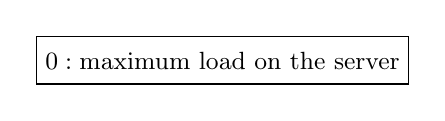
\begin{tikzpicture}
\small
\matrix[nodes={draw,minimum size=6mm}] {
  \node {$0:\textrm{maximum load on the server}$};\\
};
\end{tikzpicture}\\
\textbf{Side Effects:} none.\\
\textbf{Throws:} {\tt{}SQLException} if database failure is encountered.\\
\bottomrule
\end{tabular}
\nwenddocs{}\nwbegincode{95}\sublabel{NW18ZcDF-1O34Sj-1}\nwmargintag{{\nwtagstyle{}\subpageref{NW18ZcDF-1O34Sj-1}}}\moddef{Read: DBQueryServerLoadMax(2)~{\nwtagstyle{}\subpageref{NW18ZcDF-1O34Sj-1}}}\endmoddef\nwused{\\{NW3x1zuR-Oyob-1}}
int[] DBQueryServerLoadMax(final int sid, final int t) throws SQLException \{
  try (\LA{}Open \code{}conn\edoc{}~{\nwtagstyle{}\subpageref{NWgUSr6-JT1v9-1}}\RA{}) \{
    return PSQuery(conn, "S73", 1, sid, t);
  \} catch (SQLException e) \{
    throw e;
  \}
\}
\nwindexdefn{DBQueryServerLoadMax}{DBQueryServerLoadMax}{NW18ZcDF-1O34Sj-1}\eatline
\nwidentdefs{\\{{DBQueryServerLoadMax}{DBQueryServerLoadMax}}}\nwidentuses{\\{{PSQuery}{PSQuery}}\\{{S73}{S73}}}\nwindexuse{PSQuery}{PSQuery}{NW18ZcDF-1O34Sj-1}\nwindexuse{S73}{S73}{NW18ZcDF-1O34Sj-1}\nwendcode{}\nwbegindocs{96}\begin{tabular}{p{\textwidth}}
\toprule
\rowcolor{TableTitle}
Method \textcolor{blue}{{\tt{}\protect\nwindexuse{queryServerLoadMax}{queryServerLoadMax}{NW18ZcDF-7Mvmo-1}queryServerLoadMax}}(2) wraps {\tt{}\protect\nwindexuse{DBQueryServerLoadMax}{DBQueryServerLoadMax}{NW18ZcDF-1O34Sj-1}DBQueryServerLoadMax}(2).\\
\bottomrule
\end{tabular}
\nwenddocs{}\nwbegincode{97}\sublabel{NW18ZcDF-7Mvmo-1}\nwmargintag{{\nwtagstyle{}\subpageref{NW18ZcDF-7Mvmo-1}}}\moddef{Read: queryServerLoadMax(2)~{\nwtagstyle{}\subpageref{NW18ZcDF-7Mvmo-1}}}\endmoddef\nwused{\\{NW3x1zuR-2Rlctf-1}}
int[] queryServerLoadMax(final int sid, final int t) throws SQLException \{
  long A0 = System.currentTimeMillis();
  int[] output = this.storage.DBQueryServerLoadMax(sid, t);
  \LA{}Stats: queryServerLoadMax~{\nwtagstyle{}\subpageref{NW1n2CZQ-4eoHId-1}}\RA{}
  return output;
\}
\nosublabel{NW18ZcDF-7Mvmo-1-u1}\nwindexdefn{queryServerLoadMax}{queryServerLoadMax}{NW18ZcDF-7Mvmo-1}\eatline
\nwidentdefs{\\{{queryServerLoadMax}{queryServerLoadMax}}}\nwidentuses{\\{{DBQueryServerLoadMax}{DBQueryServerLoadMax}}}\nwindexuse{DBQueryServerLoadMax}{DBQueryServerLoadMax}{NW18ZcDF-7Mvmo-1}\nwendcode{}\nwbegindocs{98}\nwdocspar
\subsection{\texttt{DBQueryServerDistance}(1)}
\begin{tabular}{p{\textwidth}}
\toprule
\rowcolor{TableTitle}
Method \textcolor{blue}{{\tt{}\protect\nwindexuse{DBQueryServerDistance}{DBQueryServerDistance}{NW18ZcDF-cE03j-1}DBQueryServerDistance}}(1) returns the
travel distance $D(w)$ of the given server.
A {\tt{}SQLException} is thrown in case of database failure.\\
\midrule
\textbf{Parameters:} \\
\begin{tabular}{lp{116mm}}
Integer {\tt{}sid} (param. 1):&server identifier.
\end{tabular}\\
\textbf{Returns:} results of the query flattened into an integer array,
or {\tt{}null} if no results.

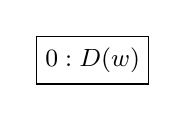
\begin{tikzpicture}
\small
\matrix[nodes={minimum size=6mm}] {
  \node[draw] {$0:D(w)$};\\
};
\end{tikzpicture}

where $w$ is the route of the given server identified by {\tt{}sid} (param. 1).\\
\textbf{Side Effects:} none.\\
\textbf{Throws:} {\tt{}SQLException} if database failure is encountered.\\
\bottomrule
\end{tabular}
\nwenddocs{}\nwbegincode{99}\sublabel{NW18ZcDF-cE03j-1}\nwmargintag{{\nwtagstyle{}\subpageref{NW18ZcDF-cE03j-1}}}\moddef{Read: DBQueryServerDistance(1)~{\nwtagstyle{}\subpageref{NW18ZcDF-cE03j-1}}}\endmoddef\nwused{\\{NW3x1zuR-Oyob-1}}
int[] DBQueryServerDistance(final int sid) throws SQLException \{
  try (\LA{}Open \code{}conn\edoc{}~{\nwtagstyle{}\subpageref{NWgUSr6-JT1v9-1}}\RA{}) \{
    return PSQuery(conn, "S104", 1, sid);
  \} catch (SQLException e) \{
    throw e;
  \}
\}
\nwindexdefn{DBQueryServerDistance}{DBQueryServerDistance}{NW18ZcDF-cE03j-1}\eatline
\nwidentdefs{\\{{DBQueryServerDistance}{DBQueryServerDistance}}}\nwidentuses{\\{{PSQuery}{PSQuery}}\\{{S104}{S104}}}\nwindexuse{PSQuery}{PSQuery}{NW18ZcDF-cE03j-1}\nwindexuse{S104}{S104}{NW18ZcDF-cE03j-1}\nwendcode{}\nwbegindocs{100}\nwdocspar
\subsection{\texttt{DBQueryServerDistanceRemaining}(2)}
\begin{tabular}{p{\textwidth}}
\toprule
\rowcolor{TableTitle}
Method \textcolor{blue}{{\tt{}\protect\nwindexuse{DBQueryServerDistanceRemaining}{DBQueryServerDistanceRemaining}{NW18ZcDF-23Wg9M-1}DBQueryServerDistanceRemaining}}(2) returns the
remaining distance $D(w_{>t})$ for the given server at the given time.
A {\tt{}SQLException} is thrown in case of database failure.\\
\midrule
\textbf{Parameters:} \\
\begin{tabular}{lp{116mm}}
Integer {\tt{}sid} (param. 1):&server identifier.\\
Integer {\tt{}t} (param. 2):&a time.\\
\end{tabular}
\textbf{Returns:} results of the query flattened into an integer array,
or {\tt{}null} if no results.

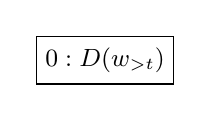
\begin{tikzpicture}
\small
\matrix[nodes={draw,minimum size=6mm}] {
  \node {$0:D(w_{>t})$};\\
};
\end{tikzpicture}

where $w_{>t}$ is the remaining route for the given server identified by {\tt{}sid} (param. 1).\\
\textbf{Side Effects:} none.\\
\textbf{Throws:} {\tt{}SQLException} if database failure is encountered.\\
\bottomrule
\end{tabular}
\nwenddocs{}\nwbegincode{101}\sublabel{NW18ZcDF-23Wg9M-1}\nwmargintag{{\nwtagstyle{}\subpageref{NW18ZcDF-23Wg9M-1}}}\moddef{Read: DBQueryServerDistanceRemaining(2)~{\nwtagstyle{}\subpageref{NW18ZcDF-23Wg9M-1}}}\endmoddef\nwused{\\{NW3x1zuR-Oyob-1}}
int[] DBQueryServerDistanceRemaining(final int sid, final int t)
throws SQLException \{
  try (\LA{}Open \code{}conn\edoc{}~{\nwtagstyle{}\subpageref{NWgUSr6-JT1v9-1}}\RA{}) \{
    return PSQuery(conn, "S142", 1, sid, t);
  \} catch (SQLException e) \{
    throw e;
  \}
\}
\nwindexdefn{DBQueryServerDistanceRemaining}{DBQueryServerDistanceRemaining}{NW18ZcDF-23Wg9M-1}\eatline
\nwidentdefs{\\{{DBQueryServerDistanceRemaining}{DBQueryServerDistanceRemaining}}}\nwidentuses{\\{{PSQuery}{PSQuery}}\\{{S142}{S142}}}\nwindexuse{PSQuery}{PSQuery}{NW18ZcDF-23Wg9M-1}\nwindexuse{S142}{S142}{NW18ZcDF-23Wg9M-1}\nwendcode{}\nwbegindocs{102}\begin{tabular}{p{\textwidth}}
\toprule
\rowcolor{TableTitle}
Method \textcolor{blue}{{\tt{}\protect\nwindexuse{queryServerDistanceRemaining}{queryServerDistanceRemaining}{NW18ZcDF-6TJm1-1}queryServerDistanceRemaining}}(2) wraps {\tt{}\protect\nwindexuse{DBQueryServerDistanceRemaining}{DBQueryServerDistanceRemaining}{NW18ZcDF-23Wg9M-1}DBQueryServerDistanceRemaining}(2).\\
\bottomrule
\end{tabular}
\nwenddocs{}\nwbegincode{103}\sublabel{NW18ZcDF-6TJm1-1}\nwmargintag{{\nwtagstyle{}\subpageref{NW18ZcDF-6TJm1-1}}}\moddef{Read: queryServerDistanceRemaining(2)~{\nwtagstyle{}\subpageref{NW18ZcDF-6TJm1-1}}}\endmoddef\nwused{\\{NW3x1zuR-2Rlctf-1}}
int[] queryServerDistanceRemaining(final int sid, final int t) throws SQLException \{
  long A0 = System.currentTimeMillis();
  int[] output = this.storage.DBQueryServerDistanceRemaining(sid, t);
  \LA{}Stats: queryServerDistanceRemaining~{\nwtagstyle{}\subpageref{NW1n2CZQ-3SSWVy-1}}\RA{}
  return output;
\}
\nosublabel{NW18ZcDF-6TJm1-1-u1}\nwindexdefn{queryServerDistanceRemaining}{queryServerDistanceRemaining}{NW18ZcDF-6TJm1-1}\eatline
\nwidentdefs{\\{{queryServerDistanceRemaining}{queryServerDistanceRemaining}}}\nwidentuses{\\{{DBQueryServerDistanceRemaining}{DBQueryServerDistanceRemaining}}}\nwindexuse{DBQueryServerDistanceRemaining}{DBQueryServerDistanceRemaining}{NW18ZcDF-6TJm1-1}\nwendcode{}\nwbegindocs{104}\nwdocspar
\subsection{\texttt{DBQueryServerDistanceCruising}(1)}
\begin{tabular}{p{\textwidth}}
\toprule
\rowcolor{TableTitle}
Method \textcolor{blue}{{\tt{}\protect\nwindexuse{DBQueryServerDistanceCruising}{DBQueryServerDistanceCruising}{NW18ZcDF-4MxFHH-1}DBQueryServerDistanceCruising}}(1) returns the
cruising distance $D^\textrm{cruise}(\mathcal{X},s)$
(Eq.~\ref{eq:cruising-distance}) of the given server.
A {\tt{}SQLException} is thrown in case of database failure.\\
\midrule
\textbf{Parameters:}\\
\begin{tabular}{lp{116mm}}
Integer {\tt{}sid} (param. 1):&server identifier.
\end{tabular}\\
\textbf{Returns:} results of the query flattened into an integer array,
or {\tt{}null} if no results.

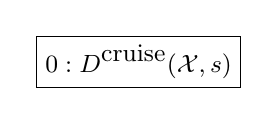
\begin{tikzpicture}
\small
\matrix[nodes={minimum size=6mm}] {
  \node[draw] {$0:D^\textrm{cruise}(\mathcal{X},s)$};\\
};
\end{tikzpicture}

where $s$ is the server identified by {\tt{}sid} (param. 1).\\
\textbf{Side Effects:} none.\\
\textbf{Throws:} {\tt{}SQLException} if database failure is encountered.\\
\bottomrule
\end{tabular}
\nwenddocs{}\nwbegincode{105}\sublabel{NW18ZcDF-4MxFHH-1}\nwmargintag{{\nwtagstyle{}\subpageref{NW18ZcDF-4MxFHH-1}}}\moddef{Read: DBQueryServerDistanceCruising(1)~{\nwtagstyle{}\subpageref{NW18ZcDF-4MxFHH-1}}}\endmoddef\nwused{\\{NW3x1zuR-Oyob-1}}
int[] DBQueryServerDistanceCruising(final int sid) throws SQLException \{
  try (\LA{}Open \code{}conn\edoc{}~{\nwtagstyle{}\subpageref{NWgUSr6-JT1v9-1}}\RA{}) \{
    return PSQuery(conn, "S106", 1, sid);
  \} catch (SQLException e) \{
    throw e;
  \}
\}
\nwindexdefn{DBQueryServerDistanceCruising}{DBQueryServerDistanceCruising}{NW18ZcDF-4MxFHH-1}\eatline
\nwidentdefs{\\{{DBQueryServerDistanceCruising}{DBQueryServerDistanceCruising}}}\nwidentuses{\\{{PSQuery}{PSQuery}}\\{{S106}{S106}}}\nwindexuse{PSQuery}{PSQuery}{NW18ZcDF-4MxFHH-1}\nwindexuse{S106}{S106}{NW18ZcDF-4MxFHH-1}\nwendcode{}\nwbegindocs{106}\nwdocspar
\subsection{\texttt{DBQueryServerDistanceService}(1)}
\begin{tabular}{p{\textwidth}}
\toprule
\rowcolor{TableTitle}
Method \textcolor{blue}{{\tt{}\protect\nwindexuse{DBQueryServerDistanceService}{DBQueryServerDistanceService}{NW18ZcDF-1qZuKY-1}DBQueryServerDistanceService}}(1) returns the
service distance $D^\textrm{service}(\mathcal{X},s)$
(Eq.~\ref{eq:service-distance}) of the given server.
A {\tt{}SQLException} is thrown in case of database failure.\\
\midrule
\textbf{Parameters:}\\
\begin{tabular}{lp{116mm}}
Integer {\tt{}sid} (param. 1):&server identifier.
\end{tabular}\\
\textbf{Returns:} results of the query flattened into an integer array,
or {\tt{}null} if no results.

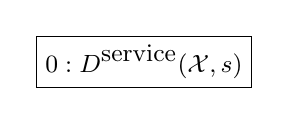
\begin{tikzpicture}
\small
\matrix[nodes={minimum size=6mm}] {
  \node[draw] {$0:D^\textrm{service}(\mathcal{X},s)$};\\
};
\end{tikzpicture}

where $s$ is the server identified by {\tt{}sid} (param. 1).\\
\textbf{Side Effects:} none.\\
\textbf{Throws:} {\tt{}SQLException} if database failure is encountered.\\
\bottomrule
\end{tabular}
\nwenddocs{}\nwbegincode{107}\sublabel{NW18ZcDF-1qZuKY-1}\nwmargintag{{\nwtagstyle{}\subpageref{NW18ZcDF-1qZuKY-1}}}\moddef{Read: DBQueryServerDistanceService(1)~{\nwtagstyle{}\subpageref{NW18ZcDF-1qZuKY-1}}}\endmoddef\nwused{\\{NW3x1zuR-Oyob-1}}
int[] DBQueryServerDistanceService(final int sid) throws SQLException \{
  try (\LA{}Open \code{}conn\edoc{}~{\nwtagstyle{}\subpageref{NWgUSr6-JT1v9-1}}\RA{}) \{
    return PSQuery(conn, "S108", 1, sid);
  \} catch (SQLException e) \{
    throw e;
  \}
\}
\nwindexdefn{DBQueryServerDistanceService}{DBQueryServerDistanceService}{NW18ZcDF-1qZuKY-1}\eatline
\nwidentdefs{\\{{DBQueryServerDistanceService}{DBQueryServerDistanceService}}}\nwidentuses{\\{{PSQuery}{PSQuery}}\\{{S108}{S108}}}\nwindexuse{PSQuery}{PSQuery}{NW18ZcDF-1qZuKY-1}\nwindexuse{S108}{S108}{NW18ZcDF-1qZuKY-1}\nwendcode{}\nwbegindocs{108}\nwdocspar
\subsection{\texttt{DBQueryServerDurationRemaining}(2)}
\begin{tabular}{p{\textwidth}}
\toprule
\rowcolor{TableTitle}
Method \textcolor{blue}{{\tt{}\protect\nwindexuse{DBQueryServerDurationRemaining}{DBQueryServerDurationRemaining}{NW18ZcDF-1aOzfQ-1}DBQueryServerDurationRemaining}}(2) returns the
remaining duration $\delta(w_{>t})$ for the given server at the given time.
A {\tt{}SQLException} is thrown in case of database failure.\\
\midrule
\textbf{Parameters:} \\
\begin{tabular}{lp{116mm}}
Integer {\tt{}sid} (param. 1):&server identifier.\\
Integer {\tt{}t} (param. 2):&a time.\\
\end{tabular}
\textbf{Returns:} results of the query flattened into an integer array,
or {\tt{}null} if no results.

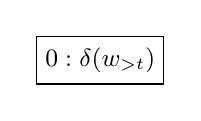
\begin{tikzpicture}
\small
\matrix[nodes={draw,minimum size=6mm}] {
  \node {$0:\delta(w_{>t})$};\\
};
\end{tikzpicture}

where $w_{>t}$ is the remaining route for the given server identified by {\tt{}sid} (param. 1).\\
\textbf{Side Effects:} none.\\
\textbf{Throws:} {\tt{}SQLException} if database failure is encountered.\\
\bottomrule
\end{tabular}
\nwenddocs{}\nwbegincode{109}\sublabel{NW18ZcDF-1aOzfQ-1}\nwmargintag{{\nwtagstyle{}\subpageref{NW18ZcDF-1aOzfQ-1}}}\moddef{Read: DBQueryServerDurationRemaining(2)~{\nwtagstyle{}\subpageref{NW18ZcDF-1aOzfQ-1}}}\endmoddef\nwused{\\{NW3x1zuR-Oyob-1}}
int[] DBQueryServerDurationRemaining(final int sid, final int t)
throws SQLException \{
  try (\LA{}Open \code{}conn\edoc{}~{\nwtagstyle{}\subpageref{NWgUSr6-JT1v9-1}}\RA{}) \{
    int[] output = PSQuery(conn, "S127", 1, sid, t);
    if (output != null) \{
      output[0] -= t;
    \}
    return output;
  \} catch (SQLException e) \{
    throw e;
  \}
\}
\nwindexdefn{DBQueryServerDurationRemaining}{DBQueryServerDurationRemaining}{NW18ZcDF-1aOzfQ-1}\eatline
\nwidentdefs{\\{{DBQueryServerDurationRemaining}{DBQueryServerDurationRemaining}}}\nwidentuses{\\{{PSQuery}{PSQuery}}\\{{S127}{S127}}}\nwindexuse{PSQuery}{PSQuery}{NW18ZcDF-1aOzfQ-1}\nwindexuse{S127}{S127}{NW18ZcDF-1aOzfQ-1}\nwendcode{}\nwbegindocs{110}\begin{tabular}{p{\textwidth}}
\toprule
\rowcolor{TableTitle}
Method \textcolor{blue}{{\tt{}\protect\nwindexuse{queryServerDurationRemaining}{queryServerDurationRemaining}{NW18ZcDF-e3rqH-1}queryServerDurationRemaining}}(2) wraps {\tt{}\protect\nwindexuse{DBQueryServerDurationRemaining}{DBQueryServerDurationRemaining}{NW18ZcDF-1aOzfQ-1}DBQueryServerDurationRemaining}(2).\\
\bottomrule
\end{tabular}
\nwenddocs{}\nwbegincode{111}\sublabel{NW18ZcDF-e3rqH-1}\nwmargintag{{\nwtagstyle{}\subpageref{NW18ZcDF-e3rqH-1}}}\moddef{Read: queryServerDurationRemaining(2)~{\nwtagstyle{}\subpageref{NW18ZcDF-e3rqH-1}}}\endmoddef\nwused{\\{NW3x1zuR-2Rlctf-1}}
int[] queryServerDurationRemaining(final int sid, final int t) throws SQLException \{
  long A0 = System.currentTimeMillis();
  int[] output = this.storage.DBQueryServerDurationRemaining(sid, t);
  \LA{}Stats: queryServerDurationRemaining~{\nwtagstyle{}\subpageref{NW1n2CZQ-2KsLG-1}}\RA{}
  return output;
\}
\nosublabel{NW18ZcDF-e3rqH-1-u1}\nwindexdefn{queryServerDurationRemaining}{queryServerDurationRemaining}{NW18ZcDF-e3rqH-1}\eatline
\nwidentdefs{\\{{queryServerDurationRemaining}{queryServerDurationRemaining}}}\nwidentuses{\\{{DBQueryServerDurationRemaining}{DBQueryServerDurationRemaining}}}\nwindexuse{DBQueryServerDurationRemaining}{DBQueryServerDurationRemaining}{NW18ZcDF-e3rqH-1}\nwendcode{}\nwbegindocs{112}\nwdocspar
\subsection{\texttt{DBQueryServerDurationTravel}(1)}
\begin{tabular}{p{\textwidth}}
\toprule
\rowcolor{TableTitle}
Method \textcolor{blue}{{\tt{}\protect\nwindexuse{DBQueryServerDurationTravel}{DBQueryServerDurationTravel}{NW18ZcDF-Sjxu7-1}DBQueryServerDurationTravel}}(1) returns the
travel duration $\delta^\textrm{travel}(\mathcal{X},r)$
(Eq.~\ref{eq:travel-duration}) of the given server.
A {\tt{}SQLException} is thrown in case of database failure.\\
\midrule
\textbf{Parameters:}\\
\begin{tabular}{lp{116mm}}
Integer {\tt{}sid} (param. 1):&server identifier.
\end{tabular}\\
\textbf{Returns:} results of the query flattened into an integer array,
or {\tt{}null} if no results.

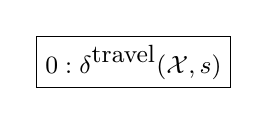
\begin{tikzpicture}
\small
\matrix[nodes={minimum size=6mm}] {
  \node[draw] {$0:\delta^\textrm{travel}(\mathcal{X},s)$};\\
};
\end{tikzpicture}

where $s$ is the server identified by {\tt{}sid} (param. 1).\\
\textbf{Side Effects:} none.\\
\textbf{Throws:} {\tt{}SQLException} if database failure is encountered.\\
\bottomrule
\end{tabular}
\nwenddocs{}\nwbegincode{113}\sublabel{NW18ZcDF-Sjxu7-1}\nwmargintag{{\nwtagstyle{}\subpageref{NW18ZcDF-Sjxu7-1}}}\moddef{Read: DBQueryServerDurationTravel(1)~{\nwtagstyle{}\subpageref{NW18ZcDF-Sjxu7-1}}}\endmoddef\nwused{\\{NW3x1zuR-Oyob-1}}
int[] DBQueryServerDurationTravel(final int sid) throws SQLException \{
  try (\LA{}Open \code{}conn\edoc{}~{\nwtagstyle{}\subpageref{NWgUSr6-JT1v9-1}}\RA{}) \{
    return PSQuery(conn, "S116", 1, sid);
  \} catch (SQLException e) \{
    throw e;
  \}
\}
\nwindexdefn{DBQueryServerDurationTravel}{DBQueryServerDurationTravel}{NW18ZcDF-Sjxu7-1}\eatline
\nwidentdefs{\\{{DBQueryServerDurationTravel}{DBQueryServerDurationTravel}}}\nwidentuses{\\{{PSQuery}{PSQuery}}\\{{S116}{S116}}}\nwindexuse{PSQuery}{PSQuery}{NW18ZcDF-Sjxu7-1}\nwindexuse{S116}{S116}{NW18ZcDF-Sjxu7-1}\nwendcode{}\nwbegindocs{114}\nwdocspar
\subsection{\texttt{DBQueryServerTimeOfDeparture}(1)}
\begin{tabular}{p{\textwidth}}
\toprule
\rowcolor{TableTitle}
Method \textcolor{blue}{{\tt{}\protect\nwindexuse{DBQueryServerTimeOfDeparture}{DBQueryServerTimeOfDeparture}{NW18ZcDF-3pEbv2-1}DBQueryServerTimeOfDeparture}}(1) returns the
departure time $t^\textrm{depart}(\mathcal{X},s)$
(Eq.~\ref{eq:departure-time}) of the given server.
A {\tt{}SQLException} is thrown in case of database failure.\\
\midrule
\textbf{Parameters:}\\
\begin{tabular}{lp{116mm}}
Integer {\tt{}sid} (param. 1):&server identifier.
\end{tabular}\\
\textbf{Returns:} results of the query flattened into an integer array,
or {\tt{}null} if no results.

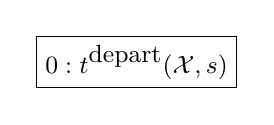
\begin{tikzpicture}
\small
\matrix[nodes={minimum size=6mm}] {
  \node[draw] {$0:t^\textrm{depart}(\mathcal{X},s)$};\\
};
\end{tikzpicture}

where $s$ is the server identified by {\tt{}sid} (param. 1).\\
\textbf{Side Effects:} none.\\
\textbf{Throws:} {\tt{}SQLException} if database failure is encountered.\\
\bottomrule
\end{tabular}
\nwenddocs{}\nwbegincode{115}\sublabel{NW18ZcDF-3pEbv2-1}\nwmargintag{{\nwtagstyle{}\subpageref{NW18ZcDF-3pEbv2-1}}}\moddef{Read: DBQueryServerTimeOfDeparture(1)~{\nwtagstyle{}\subpageref{NW18ZcDF-3pEbv2-1}}}\endmoddef\nwused{\\{NW3x1zuR-Oyob-1}}
int[] DBQueryServerTimeOfDeparture(final int sid) throws SQLException \{
  try (\LA{}Open \code{}conn\edoc{}~{\nwtagstyle{}\subpageref{NWgUSr6-JT1v9-1}}\RA{}) \{
    return PSQuery(conn, "S125", 1, sid);
  \} catch (SQLException e) \{
    throw e;
  \}
\}
\nwindexdefn{DBQueryServerTimeOfDeparture}{DBQueryServerTimeOfDeparture}{NW18ZcDF-3pEbv2-1}\eatline
\nwidentdefs{\\{{DBQueryServerTimeOfDeparture}{DBQueryServerTimeOfDeparture}}}\nwidentuses{\\{{PSQuery}{PSQuery}}\\{{S125}{S125}}}\nwindexuse{PSQuery}{PSQuery}{NW18ZcDF-3pEbv2-1}\nwindexuse{S125}{S125}{NW18ZcDF-3pEbv2-1}\nwendcode{}\nwbegindocs{116}\begin{tabular}{p{\textwidth}}
\toprule
\rowcolor{TableTitle}
Method \textcolor{blue}{{\tt{}\protect\nwindexuse{queryServerTimeOfDeparture}{queryServerTimeOfDeparture}{NW18ZcDF-3fOzh2-1}queryServerTimeOfDeparture}}(1) wraps {\tt{}\protect\nwindexuse{DBQueryServerTimeOfDeparture}{DBQueryServerTimeOfDeparture}{NW18ZcDF-3pEbv2-1}DBQueryServerTimeOfDeparture}(1).\\
\bottomrule
\end{tabular}
\nwenddocs{}\nwbegincode{117}\sublabel{NW18ZcDF-3fOzh2-1}\nwmargintag{{\nwtagstyle{}\subpageref{NW18ZcDF-3fOzh2-1}}}\moddef{Read: queryServerTimeOfDeparture(1)~{\nwtagstyle{}\subpageref{NW18ZcDF-3fOzh2-1}}}\endmoddef\nwused{\\{NW3x1zuR-2u8vSA-1}}
int[] queryServerTimeOfDeparture(final int sid) throws SQLException \{
  return storage.DBQueryServerTimeOfDeparture(sid);
\}
\nwindexdefn{queryServerTimeOfDeparture}{queryServerTimeOfDeparture}{NW18ZcDF-3fOzh2-1}\eatline
\nwidentdefs{\\{{queryServerTimeOfDeparture}{queryServerTimeOfDeparture}}}\nwidentuses{\\{{DBQueryServerTimeOfDeparture}{DBQueryServerTimeOfDeparture}}}\nwindexuse{DBQueryServerTimeOfDeparture}{DBQueryServerTimeOfDeparture}{NW18ZcDF-3fOzh2-1}\nwendcode{}\nwbegindocs{118}\nwdocspar

\subsection{\texttt{DBQueryServerTimeOfArrival}(1)}
\begin{tabular}{p{\textwidth}}
\toprule
\rowcolor{TableTitle}
Method \textcolor{blue}{{\tt{}\protect\nwindexuse{DBQueryServerTimeOfArrival}{DBQueryServerTimeOfArrival}{NW18ZcDF-4OXq2M-1}DBQueryServerTimeOfArrival}}(1) returns the
arrival time $t^\textrm{arrive}(\mathcal{X},s)$
(Eq.~\ref{eq:arrival-time}) of the given server.
A {\tt{}SQLException} is thrown in case of database failure.\\
\midrule
\textbf{Parameters:}\\
\begin{tabular}{lp{116mm}}
Integer {\tt{}sid} (param. 1):&server identifier.
\end{tabular}\\
\textbf{Returns:} results of the query flattened into an integer array,
or {\tt{}null} if no results.

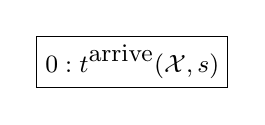
\begin{tikzpicture}
\small
\matrix[nodes={minimum size=6mm}] {
  \node[draw] {$0:t^\textrm{arrive}(\mathcal{X},s)$};\\
};
\end{tikzpicture}

where $s$ is the request identified by {\tt{}sid} (param. 1).\\
\textbf{Side Effects:} none.\\
\textbf{Throws:} {\tt{}SQLException} if database failure is encountered.\\
\bottomrule
\end{tabular}
\nwenddocs{}\nwbegincode{119}\sublabel{NW18ZcDF-4OXq2M-1}\nwmargintag{{\nwtagstyle{}\subpageref{NW18ZcDF-4OXq2M-1}}}\moddef{Read: DBQueryServerTimeOfArrival(1)~{\nwtagstyle{}\subpageref{NW18ZcDF-4OXq2M-1}}}\endmoddef\nwused{\\{NW3x1zuR-Oyob-1}}
int[] DBQueryServerTimeOfArrival(final int sid) throws SQLException \{
  try (\LA{}Open \code{}conn\edoc{}~{\nwtagstyle{}\subpageref{NWgUSr6-JT1v9-1}}\RA{}) \{
    return PSQuery(conn, "S127", 1, sid);
  \} catch (SQLException e) \{
    throw e;
  \}
\}
\nwindexdefn{DBQueryServerTimeOfArrival}{DBQueryServerTimeOfArrival}{NW18ZcDF-4OXq2M-1}\eatline
\nwidentdefs{\\{{DBQueryServerTimeOfArrival}{DBQueryServerTimeOfArrival}}}\nwidentuses{\\{{PSQuery}{PSQuery}}\\{{S127}{S127}}}\nwindexuse{PSQuery}{PSQuery}{NW18ZcDF-4OXq2M-1}\nwindexuse{S127}{S127}{NW18ZcDF-4OXq2M-1}\nwendcode{}\nwbegindocs{120}\begin{tabular}{p{\textwidth}}
\toprule
\rowcolor{TableTitle}
Method \textcolor{blue}{{\tt{}\protect\nwindexuse{queryServerTimeOfArrival}{queryServerTimeOfArrival}{NW18ZcDF-3Rabqu-1}queryServerTimeOfArrival}}(1) wraps {\tt{}\protect\nwindexuse{DBQueryServerTimeOfArrival}{DBQueryServerTimeOfArrival}{NW18ZcDF-4OXq2M-1}DBQueryServerTimeOfArrival}(1).\\
\bottomrule
\end{tabular}
\nwenddocs{}\nwbegincode{121}\sublabel{NW18ZcDF-3Rabqu-1}\nwmargintag{{\nwtagstyle{}\subpageref{NW18ZcDF-3Rabqu-1}}}\moddef{Read: queryServerTimeOfArrival(1)~{\nwtagstyle{}\subpageref{NW18ZcDF-3Rabqu-1}}}\endmoddef\nwnotused{Read:\ queryServerTimeOfArrival(1)}
int[] queryServerTimeOfArrival(final int sid) throws SQLException \{
  return storage.DBQueryServerTimeOfArrival(sid);
\}
\nwindexdefn{queryServerTimeOfArrival}{queryServerTimeOfArrival}{NW18ZcDF-3Rabqu-1}\eatline
\nwidentdefs{\\{{queryServerTimeOfArrival}{queryServerTimeOfArrival}}}\nwidentuses{\\{{DBQueryServerTimeOfArrival}{DBQueryServerTimeOfArrival}}}\nwindexuse{DBQueryServerTimeOfArrival}{DBQueryServerTimeOfArrival}{NW18ZcDF-3Rabqu-1}\nwendcode{}\nwbegindocs{122}\nwdocspar
\subsection{\texttt{DBQueryServerAssignmentsPending}(2)}
\begin{tabular}{p{\textwidth}}
\toprule
\rowcolor{TableTitle}
Method \textcolor{blue}{{\tt{}\protect\nwindexuse{DBQueryServerAssignmentsPending}{DBQueryServerAssignmentsPending}{NW18ZcDF-2nZ1VB-1}DBQueryServerAssignmentsPending}}(2) returns the
requests that will be picked up by the given server beyond the given time.
A {\tt{}SQLException} is thrown in case of database failure.\\
\midrule
\textbf{Parameters:} \\
\begin{tabular}{lp{116mm}}
Integer {\tt{}sid} (param. 1):&server identifier.\\
Integer {\tt{}t} (param. 2):&a time.\\
\end{tabular}
\textbf{Returns:} results of the query flattened into an integer array,
or {\tt{}null} if no results.

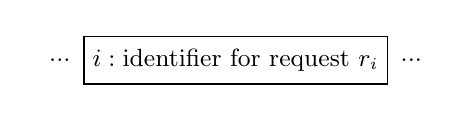
\begin{tikzpicture}
\small
\matrix[nodes={minimum size=6mm}] {
  \node {...};
 &\node[draw] {$i:\textrm{identifier for request }r_i$};
 &\node {...};\\
};
\end{tikzpicture}

where $1\leq i\leq |R^\textrm{pending}(\mathcal{X}, s, t)|$,
$r_i\in R^\textrm{pending}(\mathcal{X}, s, t)$, and
$R^\textrm{pending}(\mathcal{X}, s, t)= (R(\mathcal{X},s,H)\setminus R(\mathcal{X},s,t))$ for
time horizon $H$, server $s$ identified by {\tt{}sid} (param. 1), and time $t$ given by param. 2.\\
\textbf{Side Effects:} none.\\
\textbf{Throws:} {\tt{}SQLException} if database failure is encountered.\\
\bottomrule
\end{tabular}
\nwenddocs{}\nwbegincode{123}\sublabel{NW18ZcDF-2nZ1VB-1}\nwmargintag{{\nwtagstyle{}\subpageref{NW18ZcDF-2nZ1VB-1}}}\moddef{Read: DBQueryServerAssignmentsPending(2)~{\nwtagstyle{}\subpageref{NW18ZcDF-2nZ1VB-1}}}\endmoddef\nwused{\\{NW3x1zuR-Oyob-1}}
int[] DBQueryServerAssignmentsPending(final int sid, final int t)
throws SQLException \{
  try (\LA{}Open \code{}conn\edoc{}~{\nwtagstyle{}\subpageref{NWgUSr6-JT1v9-1}}\RA{}) \{
    return PSQuery(conn, "S100", 1, t, sid);
  \} catch (SQLException e) \{
    throw e;
  \}
\}
\nwindexdefn{DBQueryServerAssignmentsPending}{DBQueryServerAssignmentsPending}{NW18ZcDF-2nZ1VB-1}\eatline
\nwidentdefs{\\{{DBQueryServerAssignmentsPending}{DBQueryServerAssignmentsPending}}}\nwidentuses{\\{{PSQuery}{PSQuery}}\\{{S100}{S100}}}\nwindexuse{PSQuery}{PSQuery}{NW18ZcDF-2nZ1VB-1}\nwindexuse{S100}{S100}{NW18ZcDF-2nZ1VB-1}\nwendcode{}\nwbegindocs{124}\nwdocspar
\subsection{\texttt{DBQueryServerAssignmentsCompleted}(2)}
\begin{tabular}{p{\textwidth}}
\toprule
\rowcolor{TableTitle}
Method \textcolor{blue}{{\tt{}\protect\nwindexuse{DBQueryServerAssignmentsCompleted}{DBQueryServerAssignmentsCompleted}{NW18ZcDF-31osvi-1}DBQueryServerAssignmentsCompleted}}(2) returns the
requests that have been dropped off by the given server on or before the given time,
in other words $R(\mathcal{X},s,t)$ (Eq.~\ref{eq:R(X,s,t)}).
A {\tt{}SQLException} is thrown in case of database failure.\\
\midrule
\textbf{Parameters:} \\
\begin{tabular}{lp{116mm}}
Integer {\tt{}sid} (param. 1):&server identifier.\\
Integer {\tt{}t} (param. 2):&a time.\\
\end{tabular}
\textbf{Returns:} results of the query flattened into an integer array,
or {\tt{}null} if no results.

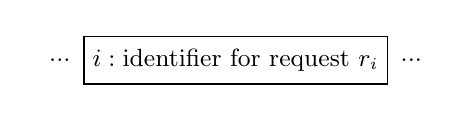
\begin{tikzpicture}
\small
\matrix[nodes={minimum size=6mm}] {
  \node {...};
 &\node[draw] {$i:\textrm{identifier for request }r_i$};
 &\node {...};\\
};
\end{tikzpicture}

where $1\leq i\leq |R(\mathcal{X},s,t)|$ and
$r_i\in R(\mathcal{X},s,t)$ for server $s$ identified by {\tt{}sid} (param. 1)
at time $t$ given by param. 2.\\
\textbf{Side Effects:} none.\\
\textbf{Throws:} {\tt{}SQLException} if database failure is encountered.\\
\bottomrule
\end{tabular}
\nwenddocs{}\nwbegincode{125}\sublabel{NW18ZcDF-31osvi-1}\nwmargintag{{\nwtagstyle{}\subpageref{NW18ZcDF-31osvi-1}}}\moddef{Read: DBQueryServerAssignmentsCompleted(2)~{\nwtagstyle{}\subpageref{NW18ZcDF-31osvi-1}}}\endmoddef\nwused{\\{NW3x1zuR-Oyob-1}}
int[] DBQueryServerAssignmentsCompleted(final int sid, final int t)
throws SQLException \{
  try (\LA{}Open \code{}conn\edoc{}~{\nwtagstyle{}\subpageref{NWgUSr6-JT1v9-1}}\RA{}) \{
    return PSQuery(conn, "S101", 1, t, sid);
  \} catch (SQLException e) \{
    throw e;
  \}
\}
\nwindexdefn{DBQueryServerAssignmentsCompleted}{DBQueryServerAssignmentsCompleted}{NW18ZcDF-31osvi-1}\eatline
\nwidentdefs{\\{{DBQueryServerAssignmentsCompleted}{DBQueryServerAssignmentsCompleted}}}\nwidentuses{\\{{PSQuery}{PSQuery}}\\{{S101}{S101}}}\nwindexuse{PSQuery}{PSQuery}{NW18ZcDF-31osvi-1}\nwindexuse{S101}{S101}{NW18ZcDF-31osvi-1}\nwendcode{}\nwbegindocs{126}\nwdocspar
\subsection{\texttt{DBQueryServersCount}(0)}
\begin{tabular}{p{\textwidth}}
\toprule
\rowcolor{TableTitle}
Method \textcolor{blue}{{\tt{}DBQueryCountSevers}}(0) returns the total number
of servers in Table S.
A {\tt{}SQLException} is thrown in case of database failure.\\
\midrule
\textbf{Parameters:} none.\\
\textbf{Returns:} results of the query flattened into an integer array, or
{\tt{}null} if no results.

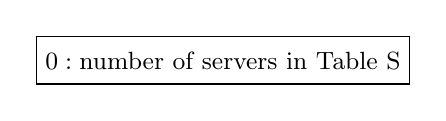
\begin{tikzpicture}
\small
\matrix[nodes={draw,minimum size=6mm}] {
  \node {$0:\textrm{number of servers in Table S}$};\\
};
\end{tikzpicture}\\
\textbf{Side Effects:} none.\\
\textbf{Throws:} {\tt{}SQLException} if database failure is encountered.\\
\bottomrule
\end{tabular}
\nwenddocs{}\nwbegincode{127}\sublabel{NW18ZcDF-23ZhQ2-1}\nwmargintag{{\nwtagstyle{}\subpageref{NW18ZcDF-23ZhQ2-1}}}\moddef{Read: DBQueryServersCount(0)~{\nwtagstyle{}\subpageref{NW18ZcDF-23ZhQ2-1}}}\endmoddef\nwused{\\{NW3x1zuR-Oyob-1}}
int[] DBQueryServersCount() throws SQLException \{
  try (\LA{}Open \code{}conn\edoc{}~{\nwtagstyle{}\subpageref{NWgUSr6-JT1v9-1}}\RA{}) \{
    return this.PSQuery(conn, "S66", 1);
  \} catch (SQLException e) \{
    throw e;
  \}
\}
\nwindexdefn{DBQueryServersCount}{DBQueryServersCount}{NW18ZcDF-23ZhQ2-1}\eatline
\nwidentdefs{\\{{DBQueryServersCount}{DBQueryServersCount}}}\nwidentuses{\\{{PSQuery}{PSQuery}}\\{{S66}{S66}}}\nwindexuse{PSQuery}{PSQuery}{NW18ZcDF-23ZhQ2-1}\nwindexuse{S66}{S66}{NW18ZcDF-23ZhQ2-1}\nwendcode{}\nwbegindocs{128}\begin{tabular}{p{\textwidth}}
\toprule
\rowcolor{TableTitle}
Method \textcolor{blue}{{\tt{}\protect\nwindexuse{queryServersCount}{queryServersCount}{NW18ZcDF-3YlcHc-1}queryServersCount}}(0) wraps {\tt{}\protect\nwindexuse{DBQueryServersCount}{DBQueryServersCount}{NW18ZcDF-23ZhQ2-1}DBQueryServersCount}(0).\\
\bottomrule
\end{tabular}
\nwenddocs{}\nwbegincode{129}\sublabel{NW18ZcDF-3YlcHc-1}\nwmargintag{{\nwtagstyle{}\subpageref{NW18ZcDF-3YlcHc-1}}}\moddef{Read: queryServersCount(0)~{\nwtagstyle{}\subpageref{NW18ZcDF-3YlcHc-1}}}\endmoddef\nwused{\\{NW3x1zuR-2u8vSA-1}}
int[] queryServersCount() throws SQLException \{
  return storage.DBQueryServersCount();
\}
\nwindexdefn{queryServersCount}{queryServersCount}{NW18ZcDF-3YlcHc-1}\eatline
\nwidentdefs{\\{{queryServersCount}{queryServersCount}}}\nwidentuses{\\{{DBQueryServersCount}{DBQueryServersCount}}}\nwindexuse{DBQueryServersCount}{DBQueryServersCount}{NW18ZcDF-3YlcHc-1}\nwendcode{}\nwbegindocs{130}\nwdocspar
\subsection{\texttt{DBQueryServersActive}(1)}
\begin{tabular}{p{\textwidth}}
\toprule
\rowcolor{TableTitle}
Method \textcolor{blue}{{\tt{}\protect\nwindexuse{DBQueryServersActive}{DBQueryServersActive}{NW18ZcDF-3NWzRo-1}DBQueryServersActive}}(1) returns the identifiers
of the active servers at the given time. A server is ``active'' if its
service has not ended.
A {\tt{}SQLException} is thrown in case of database failure.\\
\midrule
\textbf{Parameters:} \\
\begin{tabular}{lp{116mm}}
Integer {\tt{}t} (param. 1):&a time
\end{tabular}\\
\textbf{Returns:} results of the query flattened into an integer array, or
{\tt{}null} if no results.

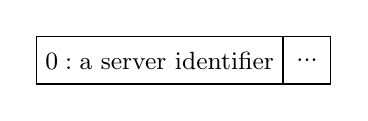
\begin{tikzpicture}
\small
\matrix[nodes={draw,minimum size=6mm}] {
  \node {$0:\textrm{a server identifier}$};
 &\node {...};\\
};
\end{tikzpicture}\\
\textbf{Side Effects:} none.\\
\textbf{Throws:} {\tt{}SQLException} if database failure is encountered.\\
\bottomrule
\end{tabular}
\nwenddocs{}\nwbegincode{131}\sublabel{NW18ZcDF-3NWzRo-1}\nwmargintag{{\nwtagstyle{}\subpageref{NW18ZcDF-3NWzRo-1}}}\moddef{Read: DBQueryServersActive(1)~{\nwtagstyle{}\subpageref{NW18ZcDF-3NWzRo-1}}}\endmoddef\nwused{\\{NW3x1zuR-Oyob-1}}
int[] DBQueryServersActive(final int t) throws SQLException \{
  try (\LA{}Open \code{}conn\edoc{}~{\nwtagstyle{}\subpageref{NWgUSr6-JT1v9-1}}\RA{}) \{
    return this.PSQuery(conn, "S134", 1, t, t, t);
  \} catch (SQLException e) \{
    throw e;
  \}
\}
\nwindexdefn{DBQueryServersActive}{DBQueryServersActive}{NW18ZcDF-3NWzRo-1}\eatline
\nwidentdefs{\\{{DBQueryServersActive}{DBQueryServersActive}}}\nwidentuses{\\{{PSQuery}{PSQuery}}\\{{S134}{S134}}}\nwindexuse{PSQuery}{PSQuery}{NW18ZcDF-3NWzRo-1}\nwindexuse{S134}{S134}{NW18ZcDF-3NWzRo-1}\nwendcode{}

\nwixlogsorted{c}{{..round to nearest meter}{NW3zOIuJ-1p0YRJ-1}{\nwixu{NW3zOIuJ-4DIogh-1}\nwixd{NW3zOIuJ-1p0YRJ-1}}}%
\nwixlogsorted{c}{{..skip header rows}{NW2ZDXo8-4FZ4vu-1}{\nwixu{NW2ZDXo8-1LrOKh-1}\nwixd{NW2ZDXo8-4FZ4vu-1}}}%
\nwixlogsorted{c}{{\code{}Client\edoc{} constructor}{NW2q3QGT-2crckK-1}{\nwixu{NW2q3QGT-bpC9O-1}\nwixd{NW2q3QGT-2crckK-1}}}%
\nwixlogsorted{c}{{\code{}Client\edoc{} member variables}{NW1n2CZQ-3qCSiR-1}{\nwixd{NW1n2CZQ-3qCSiR-1}\nwixu{NW2q3QGT-bpC9O-1}\nwixd{NW2q3QGT-3qCSiR-2}}}%
\nwixlogsorted{c}{{\code{}Client\edoc{} methods}{NW3x1zuR-1aFZ2n-1}{\nwixd{NW3x1zuR-1aFZ2n-1}\nwixd{NW3x1zuR-1aFZ2n-2}\nwixd{NW3x1zuR-1aFZ2n-3}\nwixd{NW1n2CZQ-1aFZ2n-4}\nwixu{NW2q3QGT-bpC9O-1}}}%
\nwixlogsorted{c}{{\code{}Client\edoc{} register JMX monitor}{NW1n2CZQ-3LVQBe-1}{\nwixd{NW1n2CZQ-3LVQBe-1}\nwixu{NW2q3QGT-2crckK-1}}}%
\nwixlogsorted{c}{{\code{}Communicator\edoc{} constructor}{NWvbkzY-1EwPlT-1}{\nwixu{NWvbkzY-1uGZre-1}\nwixd{NWvbkzY-1EwPlT-1}}}%
\nwixlogsorted{c}{{\code{}Communicator\edoc{} member variables}{NW1n2CZQ-18oERh-1}{\nwixd{NW1n2CZQ-18oERh-1}\nwixu{NWvbkzY-1uGZre-1}\nwixd{NWvbkzY-18oERh-2}}}%
\nwixlogsorted{c}{{\code{}Communicator\edoc{} methods}{NW3x1zuR-2Rlctf-1}{\nwixd{NW3x1zuR-2Rlctf-1}\nwixd{NW3x1zuR-2Rlctf-2}\nwixd{NW3x1zuR-2Rlctf-3}\nwixd{NW1n2CZQ-2Rlctf-4}\nwixu{NWvbkzY-1uGZre-1}}}%
\nwixlogsorted{c}{{\code{}Communicator\edoc{} register JMX monitor}{NW1n2CZQ-VjorX-1}{\nwixd{NW1n2CZQ-VjorX-1}\nwixu{NWvbkzY-1EwPlT-1}}}%
\nwixlogsorted{c}{{\code{}Controller\edoc{} constructor}{NW2ZDXo8-3AyyZG-1}{\nwixu{NW2ZDXo8-34QoYM-1}\nwixd{NW2ZDXo8-3AyyZG-1}}}%
\nwixlogsorted{c}{{\code{}Controller\edoc{} member variables}{NW1n2CZQ-3yXfwG-1}{\nwixd{NW1n2CZQ-3yXfwG-1}\nwixu{NW2ZDXo8-34QoYM-1}\nwixd{NW2ZDXo8-3yXfwG-2}}}%
\nwixlogsorted{c}{{\code{}Controller\edoc{} methods}{NW3x1zuR-2u8vSA-1}{\nwixd{NW3x1zuR-2u8vSA-1}\nwixd{NW3x1zuR-2u8vSA-2}\nwixd{NW3x1zuR-2u8vSA-3}\nwixd{NW1n2CZQ-2u8vSA-4}\nwixu{NW2ZDXo8-34QoYM-1}}}%
\nwixlogsorted{c}{{\code{}Controller\edoc{} register JMX monitor}{NW1n2CZQ-3vTTnp-1}{\nwixd{NW1n2CZQ-3vTTnp-1}\nwixu{NW2ZDXo8-3AyyZG-1}}}%
\nwixlogsorted{c}{{\code{}DesktopController\edoc{} member variables}{NWn0bN8-2iHsHO-1}{\nwixu{NWn0bN8-4ScqTl-1}\nwixd{NWn0bN8-2iHsHO-1}\nwixd{NWn0bN8-2iHsHO-2}\nwixd{NWn0bN8-2iHsHO-3}\nwixd{NWn0bN8-2iHsHO-4}\nwixd{NWn0bN8-2iHsHO-5}\nwixd{NWn0bN8-2iHsHO-6}\nwixd{NWn0bN8-2iHsHO-7}\nwixd{NWn0bN8-2iHsHO-8}\nwixd{NWn0bN8-2iHsHO-9}\nwixd{NWn0bN8-2iHsHO-A}\nwixd{NWn0bN8-2iHsHO-B}}}%
\nwixlogsorted{c}{{\code{}DesktopController\edoc{} methods}{NW3x1zuR-14uWYi-1}{\nwixd{NW3x1zuR-14uWYi-1}\nwixd{NW3x1zuR-14uWYi-2}\nwixd{NW3x1zuR-14uWYi-3}\nwixu{NWn0bN8-4ScqTl-1}}}%
\nwixlogsorted{c}{{\code{}Storage\edoc{} constructor}{NW27XAxz-36NvOs-1}{\nwixu{NW27XAxz-203Bbj-1}\nwixd{NW27XAxz-36NvOs-1}}}%
\nwixlogsorted{c}{{\code{}Storage\edoc{} member variables}{NW27XAxz-17yXws-1}{\nwixu{NW27XAxz-203Bbj-1}\nwixd{NW27XAxz-17yXws-1}\nwixd{NW27XAxz-17yXws-2}\nwixd{NW27XAxz-17yXws-3}\nwixd{NW27XAxz-17yXws-4}}}%
\nwixlogsorted{c}{{\code{}Storage\edoc{} methods}{NW3x1zuR-Oyob-1}{\nwixd{NW3x1zuR-Oyob-1}\nwixd{NW3x1zuR-Oyob-2}\nwixd{NW3x1zuR-Oyob-3}\nwixu{NW27XAxz-203Bbj-1}}}%
\nwixlogsorted{c}{{\code{}Storage\edoc{} register JMX monitor}{NW1n2CZQ-4R4Mml-1}{\nwixd{NW1n2CZQ-4R4Mml-1}\nwixu{NW27XAxz-36NvOs-1}}}%
\nwixlogsorted{c}{{\code{}Tools\edoc{} constructor}{NW3zOIuJ-t47ol-1}{\nwixu{NW3zOIuJ-2Vh5vZ-1}\nwixd{NW3zOIuJ-t47ol-1}}}%
\nwixlogsorted{c}{{\code{}Tools\edoc{} member variables}{NW3zOIuJ-2Qlw5e-1}{\nwixu{NW3zOIuJ-2Vh5vZ-1}\nwixd{NW3zOIuJ-2Qlw5e-1}}}%
\nwixlogsorted{c}{{\code{}Tools\edoc{} methods}{NW3x1zuR-3QhyAk-1}{\nwixd{NW3x1zuR-3QhyAk-1}\nwixd{NW3x1zuR-3QhyAk-2}\nwixd{NW3x1zuR-3QhyAk-3}\nwixu{NW3zOIuJ-2Vh5vZ-1}}}%
\nwixlogsorted{c}{{\code{}Traffic\edoc{} constructor}{NW24od5B-4V88df-1}{\nwixu{NW24od5B-2eR0nK-1}\nwixd{NW24od5B-4V88df-1}}}%
\nwixlogsorted{c}{{\code{}Traffic\edoc{} member variables}{NW24od5B-1j90we-1}{\nwixu{NW24od5B-2eR0nK-1}\nwixd{NW24od5B-1j90we-1}}}%
\nwixlogsorted{c}{{\code{}Traffic\edoc{} methods}{NW3x1zuR-1sp72R-1}{\nwixd{NW3x1zuR-1sp72R-1}\nwixd{NW3x1zuR-1sp72R-2}\nwixd{NW3x1zuR-1sp72R-3}\nwixu{NW24od5B-2eR0nK-1}}}%
\nwixlogsorted{c}{{actionAbout(1)}{NWn0bN8-3NAmly-1}{\nwixu{NW3x1zuR-14uWYi-3}\nwixd{NWn0bN8-3NAmly-1}}}%
\nwixlogsorted{c}{{actionClient(1)}{NWn0bN8-4G0CtX-1}{\nwixu{NW3x1zuR-14uWYi-3}\nwixd{NWn0bN8-4G0CtX-1}}}%
\nwixlogsorted{c}{{actionGitHub(1)}{NWn0bN8-1K1K6E-1}{\nwixu{NW3x1zuR-14uWYi-3}\nwixd{NWn0bN8-1K1K6E-1}}}%
\nwixlogsorted{c}{{actionGtree(1)}{NWn0bN8-18974H-1}{\nwixu{NW3x1zuR-14uWYi-3}\nwixd{NWn0bN8-18974H-1}}}%
\nwixlogsorted{c}{{actionLoad(1)}{NWn0bN8-2dDAtx-1}{\nwixu{NW3x1zuR-14uWYi-3}\nwixd{NWn0bN8-2dDAtx-1}}}%
\nwixlogsorted{c}{{actionNew(1)}{NWn0bN8-T7Xhs-1}{\nwixu{NW3x1zuR-14uWYi-3}\nwixd{NWn0bN8-T7Xhs-1}}}%
\nwixlogsorted{c}{{actionProb(1)}{NWn0bN8-ZrzWj-1}{\nwixu{NW3x1zuR-14uWYi-3}\nwixd{NWn0bN8-ZrzWj-1}}}%
\nwixlogsorted{c}{{actionQuit(1)}{NWn0bN8-2vzGSf-1}{\nwixu{NW3x1zuR-14uWYi-3}\nwixd{NWn0bN8-2vzGSf-1}}}%
\nwixlogsorted{c}{{actionRecordMousePress(1)}{NWn0bN8-3GqJTd-1}{\nwixu{NW3x1zuR-14uWYi-3}\nwixd{NWn0bN8-3GqJTd-1}}}%
\nwixlogsorted{c}{{actionRoad(1)}{NWn0bN8-2qwznl-1}{\nwixu{NW3x1zuR-14uWYi-3}\nwixd{NWn0bN8-2qwznl-1}}}%
\nwixlogsorted{c}{{actionStartRealtime(1)}{NWn0bN8-1u3CLd-1}{\nwixu{NW3x1zuR-14uWYi-3}\nwixd{NWn0bN8-1u3CLd-1}}}%
\nwixlogsorted{c}{{actionStartSequential(1)}{NWn0bN8-2DyoOl-1}{\nwixu{NW3x1zuR-14uWYi-3}\nwixd{NWn0bN8-2DyoOl-1}}}%
\nwixlogsorted{c}{{actionStop(1)}{NWn0bN8-27hSI5-1}{\nwixu{NW3x1zuR-14uWYi-3}\nwixd{NWn0bN8-27hSI5-1}}}%
\nwixlogsorted{c}{{actionTranslateCanvas(1)}{NWn0bN8-10utze-1}{\nwixu{NW3x1zuR-14uWYi-3}\nwixd{NWn0bN8-10utze-1}}}%
\nwixlogsorted{c}{{Add charts to chart containers}{NWn0bN8-35Xz53-1}{\nwixd{NWn0bN8-35Xz53-1}\nwixu{NWn0bN8-2DyoOl-1}}}%
\nwixlogsorted{c}{{addRequest(1)}{NW2q3QGT-3oJ3LB-1}{\nwixu{NW3x1zuR-1aFZ2n-3}\nwixd{NW2q3QGT-3oJ3LB-1}}}%
\nwixlogsorted{c}{{Admin: cacheRoadNetworkFromDB(0)}{NWgUSr6-fYeVD-1}{\nwixu{NW3x1zuR-2u8vSA-3}\nwixd{NWgUSr6-fYeVD-1}}}%
\nwixlogsorted{c}{{Admin: cacheUsersFromDB(0)}{NWgUSr6-3L7Lsf-1}{\nwixu{NW3x1zuR-2u8vSA-3}\nwixd{NWgUSr6-3L7Lsf-1}}}%
\nwixlogsorted{c}{{Admin: instanceClose(0)}{NWgUSr6-1Uv5LH-1}{\nwixu{NW3x1zuR-2u8vSA-3}\nwixd{NWgUSr6-1Uv5LH-1}}}%
\nwixlogsorted{c}{{Admin: instanceExport(1)}{NWgUSr6-41pCsM-1}{\nwixu{NW3x1zuR-2u8vSA-3}\nwixd{NWgUSr6-41pCsM-1}}}%
\nwixlogsorted{c}{{Admin: instanceInitialize(0)}{NWgUSr6-3zrPv1-1}{\nwixu{NW3x1zuR-2u8vSA-3}\nwixd{NWgUSr6-3zrPv1-1}}}%
\nwixlogsorted{c}{{Admin: instanceLoad(1)}{NWgUSr6-1xqWgs-1}{\nwixu{NW3x1zuR-2u8vSA-3}\nwixd{NWgUSr6-1xqWgs-1}}}%
\nwixlogsorted{c}{{Admin: instanceNew(0)}{NWgUSr6-7iNDJ-1}{\nwixu{NW3x1zuR-2u8vSA-3}\nwixd{NWgUSr6-7iNDJ-1}}}%
\nwixlogsorted{c}{{Admin: JargoCacheRoadNetworkFromDB(0)}{NWgUSr6-1Dy9Ql-1}{\nwixu{NW3x1zuR-Oyob-3}\nwixd{NWgUSr6-1Dy9Ql-1}\nwixd{NWgUSr6-1Dy9Ql-2}\nwixd{NWgUSr6-1Dy9Ql-3}\nwixd{NWgUSr6-1Dy9Ql-4}\nwixd{NWgUSr6-1Dy9Ql-5}}}%
\nwixlogsorted{c}{{Admin: JargoCacheUsersFromDB(0)}{NWgUSr6-3RkokI-1}{\nwixu{NW3x1zuR-Oyob-3}\nwixd{NWgUSr6-3RkokI-1}\nwixd{NWgUSr6-3RkokI-2}\nwixd{NWgUSr6-3RkokI-3}\nwixd{NWgUSr6-3RkokI-4}\nwixd{NWgUSr6-3RkokI-5}}}%
\nwixlogsorted{c}{{Admin: JargoInstanceClose(0)}{NWgUSr6-46VGhz-1}{\nwixu{NW3x1zuR-Oyob-3}\nwixd{NWgUSr6-46VGhz-1}}}%
\nwixlogsorted{c}{{Admin: JargoInstanceExport(1)}{NWgUSr6-4UssFH-1}{\nwixu{NW3x1zuR-Oyob-3}\nwixd{NWgUSr6-4UssFH-1}}}%
\nwixlogsorted{c}{{Admin: JargoInstanceInitialize(0)}{NWgUSr6-RmKLy-1}{\nwixu{NW3x1zuR-Oyob-3}\nwixd{NWgUSr6-RmKLy-1}}}%
\nwixlogsorted{c}{{Admin: JargoInstanceLoad(1)}{NWgUSr6-2ccHxN-1}{\nwixu{NW3x1zuR-Oyob-3}\nwixd{NWgUSr6-2ccHxN-1}}}%
\nwixlogsorted{c}{{Admin: JargoInstanceNew(0)}{NWgUSr6-2umFNk-1}{\nwixu{NW3x1zuR-Oyob-3}\nwixd{NWgUSr6-2umFNk-1}}}%
\nwixlogsorted{c}{{Admin: JargoSetupDriver(0)}{NWgUSr6-2KJvvu-1}{\nwixu{NW3x1zuR-Oyob-3}\nwixd{NWgUSr6-2KJvvu-1}}}%
\nwixlogsorted{c}{{Admin: JargoSetupPreparedStatements(0)}{NWgUSr6-1dEGs4-1}{\nwixu{NW3x1zuR-Oyob-3}\nwixd{NWgUSr6-1dEGs4-1}}}%
\nwixlogsorted{c}{{Admin: PSAdd(2..)}{NWgUSr6-1X4ymL-1}{\nwixu{NW3x1zuR-Oyob-3}\nwixd{NWgUSr6-1X4ymL-1}}}%
\nwixlogsorted{c}{{Admin: PSCreate(2)}{NWgUSr6-47iuYD-1}{\nwixu{NW3x1zuR-Oyob-3}\nwixd{NWgUSr6-47iuYD-1}}}%
\nwixlogsorted{c}{{Admin: PSQuery(3..)}{NWgUSr6-yHOIP-1}{\nwixu{NW3x1zuR-Oyob-3}\nwixd{NWgUSr6-yHOIP-1}}}%
\nwixlogsorted{c}{{Admin: PSSubmit(1..)}{NWgUSr6-1S1xBT-1}{\nwixu{NW3x1zuR-Oyob-3}\nwixd{NWgUSr6-1S1xBT-1}}}%
\nwixlogsorted{c}{{Apply traffic to route, sched}{NW32V2DP-UeHS0-1}{\nwixd{NW32V2DP-UeHS0-1}\nwixu{NW32V2DP-3PimUR-1}\nwixu{NW32V2DP-42pL1g-1}\nwixu{NW32V2DP-3O61Nf-1}}}%
\nwixlogsorted{c}{{apply(3)}{NW24od5B-14vbUh-1}{\nwixu{NW3x1zuR-1sp72R-3}\nwixd{NW24od5B-14vbUh-1}}}%
\nwixlogsorted{c}{{Check time window violation}{NW32V2DP-3kBClV-1}{\nwixd{NW32V2DP-3kBClV-1}\nwixu{NW32V2DP-3PimUR-1}\nwixu{NW32V2DP-42pL1g-1}\nwixu{NW32V2DP-3O61Nf-1}}}%
\nwixlogsorted{c}{{Client.java}{NW2q3QGT-bpC9O-1}{\nwixd{NW2q3QGT-bpC9O-1}}}%
\nwixlogsorted{c}{{Client.java preamble}{NW2q3QGT-xBgX1-1}{\nwixu{NW2q3QGT-bpC9O-1}\nwixd{NW2q3QGT-xBgX1-1}\nwixd{NW2q3QGT-xBgX1-2}\nwixd{NW2q3QGT-xBgX1-3}}}%
\nwixlogsorted{c}{{collectServerLocations(1)}{NW2q3QGT-k7vZ4-1}{\nwixu{NW3x1zuR-1aFZ2n-3}\nwixd{NW2q3QGT-k7vZ4-1}}}%
\nwixlogsorted{c}{{Communicator.java}{NWvbkzY-1uGZre-1}{\nwixd{NWvbkzY-1uGZre-1}}}%
\nwixlogsorted{c}{{Communicator.java preamble}{NWvbkzY-3IAuyF-1}{\nwixu{NWvbkzY-1uGZre-1}\nwixd{NWvbkzY-3IAuyF-1}\nwixd{NWvbkzY-3IAuyF-2}}}%
\nwixlogsorted{c}{{computeDuration(2)}{NW3zOIuJ-3wcav7-1}{\nwixu{NW3x1zuR-3QhyAk-3}\nwixd{NW3zOIuJ-3wcav7-1}}}%
\nwixlogsorted{c}{{computeHaversine(2)}{NW3zOIuJ-4DaU51-1}{\nwixu{NW3x1zuR-3QhyAk-3}\nwixd{NW3zOIuJ-4DaU51-1}}}%
\nwixlogsorted{c}{{computeHaversine(4)}{NW3zOIuJ-4DIogh-1}{\nwixu{NW3x1zuR-3QhyAk-3}\nwixd{NW3zOIuJ-4DIogh-1}}}%
\nwixlogsorted{c}{{computeRoute(3)}{NW3zOIuJ-AzxgG-1}{\nwixu{NW3x1zuR-3QhyAk-3}\nwixd{NW3zOIuJ-AzxgG-1}}}%
\nwixlogsorted{c}{{computeShortestPath(2)}{NW3zOIuJ-4dTO5e-1}{\nwixu{NW3x1zuR-3QhyAk-3}\nwixd{NW3zOIuJ-4dTO5e-1}}}%
\nwixlogsorted{c}{{computeShortestPathDistance(2)}{NW3zOIuJ-1zhqNP-1}{\nwixu{NW3x1zuR-3QhyAk-3}\nwixd{NW3zOIuJ-1zhqNP-1}}}%
\nwixlogsorted{c}{{Container objects}{NW2ZDXo8-OUspt-1}{\nwixu{NW2ZDXo8-3yXfwG-2}\nwixd{NW2ZDXo8-OUspt-1}}}%
\nwixlogsorted{c}{{Controller.java}{NW2ZDXo8-34QoYM-1}{\nwixd{NW2ZDXo8-34QoYM-1}}}%
\nwixlogsorted{c}{{Controller.java preamble}{NW2ZDXo8-m6OHq-1}{\nwixu{NW2ZDXo8-34QoYM-1}\nwixd{NW2ZDXo8-m6OHq-1}\nwixd{NW2ZDXo8-m6OHq-2}\nwixd{NW2ZDXo8-m6OHq-3}\nwixd{NW2ZDXo8-m6OHq-4}\nwixd{NW2ZDXo8-m6OHq-5}\nwixd{NW2ZDXo8-m6OHq-6}}}%
\nwixlogsorted{c}{{Create Table CPD statement}{NW3jn8Pl-q5ofx-1}{\nwixd{NW3jn8Pl-q5ofx-1}\nwixu{NWgUSr6-RmKLy-1}}}%
\nwixlogsorted{c}{{Create Table CQ statement}{NW3jn8Pl-2YsMAX-1}{\nwixd{NW3jn8Pl-2YsMAX-1}\nwixu{NWgUSr6-RmKLy-1}}}%
\nwixlogsorted{c}{{Create Table CW statement}{NW3jn8Pl-2HehGp-1}{\nwixd{NW3jn8Pl-2HehGp-1}\nwixu{NWgUSr6-RmKLy-1}}}%
\nwixlogsorted{c}{{Create Table E statement}{NW3jn8Pl-2WHSWQ-1}{\nwixd{NW3jn8Pl-2WHSWQ-1}\nwixu{NWgUSr6-RmKLy-1}}}%
\nwixlogsorted{c}{{Create Table PD statement}{NW3jn8Pl-1aGcZB-1}{\nwixd{NW3jn8Pl-1aGcZB-1}\nwixu{NWgUSr6-RmKLy-1}}}%
\nwixlogsorted{c}{{Create Table R statement}{NW3jn8Pl-Uo9HJ-1}{\nwixd{NW3jn8Pl-Uo9HJ-1}\nwixu{NWgUSr6-RmKLy-1}}}%
\nwixlogsorted{c}{{Create Table S statement}{NW3jn8Pl-2D0DN7-1}{\nwixd{NW3jn8Pl-2D0DN7-1}\nwixu{NWgUSr6-RmKLy-1}}}%
\nwixlogsorted{c}{{Create Table UB statement}{NW3jn8Pl-3QSM5L-1}{\nwixd{NW3jn8Pl-3QSM5L-1}\nwixu{NWgUSr6-RmKLy-1}}}%
\nwixlogsorted{c}{{Create Table UD statement}{NW3jn8Pl-1OVMyH-1}{\nwixd{NW3jn8Pl-1OVMyH-1}\nwixu{NWgUSr6-RmKLy-1}}}%
\nwixlogsorted{c}{{Create Table UE statement}{NW3jn8Pl-sBCgz-1}{\nwixd{NW3jn8Pl-sBCgz-1}\nwixu{NWgUSr6-RmKLy-1}}}%
\nwixlogsorted{c}{{Create Table UL statement}{NW3jn8Pl-3Q8NSk-1}{\nwixd{NW3jn8Pl-3Q8NSk-1}\nwixu{NWgUSr6-RmKLy-1}}}%
\nwixlogsorted{c}{{Create Table UO statement}{NW3jn8Pl-qCW00-1}{\nwixd{NW3jn8Pl-qCW00-1}\nwixu{NWgUSr6-RmKLy-1}}}%
\nwixlogsorted{c}{{Create Table UQ statement}{NW3jn8Pl-llmAG-1}{\nwixd{NW3jn8Pl-llmAG-1}\nwixu{NWgUSr6-RmKLy-1}}}%
\nwixlogsorted{c}{{Create Table V statement}{NW3jn8Pl-RzwV3-1}{\nwixd{NW3jn8Pl-RzwV3-1}\nwixu{NWgUSr6-RmKLy-1}}}%
\nwixlogsorted{c}{{Create Table W statement}{NW3jn8Pl-2FnbXJ-1}{\nwixd{NW3jn8Pl-2FnbXJ-1}\nwixu{NWgUSr6-RmKLy-1}}}%
\nwixlogsorted{c}{{Create View assignments statement (Eq.~\ref{eq:assignments})}{NW3jn8Pl-4DFJnJ-1}{\nwixd{NW3jn8Pl-4DFJnJ-1}\nwixu{NWgUSr6-RmKLy-1}}}%
\nwixlogsorted{c}{{Create View assignments\_r statement (Eq.~\ref{eq:assigned-requests})}{NW3jn8Pl-4Me5rv-1}{\nwixd{NW3jn8Pl-4Me5rv-1}\nwixu{NWgUSr6-RmKLy-1}}}%
\nwixlogsorted{c}{{Create View dist\_base statement (Eq.~\ref{eq:base-distance})}{NW3jn8Pl-Xwf4i-1}{\nwixd{NW3jn8Pl-Xwf4i-1}\nwixu{NWgUSr6-RmKLy-1}}}%
\nwixlogsorted{c}{{Create View dist\_r\_base statement}{NW3jn8Pl-2qZ1kZ-1}{\nwixd{NW3jn8Pl-2qZ1kZ-1}\nwixu{NWgUSr6-RmKLy-1}}}%
\nwixlogsorted{c}{{Create View dist\_r\_detour statement (Eq.~\ref{eq:detour-distance})}{NW3jn8Pl-4OnMrk-1}{\nwixd{NW3jn8Pl-4OnMrk-1}\nwixu{NWgUSr6-RmKLy-1}}}%
\nwixlogsorted{c}{{Create View dist\_r\_transit statement (Eq.~\ref{eq:transit-distance})}{NW3jn8Pl-eXH6J-1}{\nwixd{NW3jn8Pl-eXH6J-1}\nwixu{NWgUSr6-RmKLy-1}}}%
\nwixlogsorted{c}{{Create View dist\_r\_unassigned statement}{NW3jn8Pl-20Wo4P-1}{\nwixd{NW3jn8Pl-20Wo4P-1}\nwixu{NWgUSr6-RmKLy-1}}}%
\nwixlogsorted{c}{{Create View dist\_s\_base statement}{NW3jn8Pl-15VZds-1}{\nwixd{NW3jn8Pl-15VZds-1}\nwixu{NWgUSr6-RmKLy-1}}}%
\nwixlogsorted{c}{{Create View dist\_s\_cruising statement (Eq.~\ref{eq:cruising-distance})}{NW3jn8Pl-sPBsa-1}{\nwixd{NW3jn8Pl-sPBsa-1}\nwixu{NWgUSr6-RmKLy-1}}}%
\nwixlogsorted{c}{{Create View dist\_s\_service statement (Eq.~\ref{eq:service-distance})}{NW3jn8Pl-21lyOa-1}{\nwixd{NW3jn8Pl-21lyOa-1}\nwixu{NWgUSr6-RmKLy-1}}}%
\nwixlogsorted{c}{{Create View dist\_s\_travel statement}{NW3jn8Pl-I0bnu-1}{\nwixd{NW3jn8Pl-I0bnu-1}\nwixu{NWgUSr6-RmKLy-1}}}%
\nwixlogsorted{c}{{Create View dur\_r\_pickup statement (Eq.~\ref{eq:pick-up delay})}{NW3jn8Pl-34NkTM-1}{\nwixd{NW3jn8Pl-34NkTM-1}\nwixu{NWgUSr6-RmKLy-1}}}%
\nwixlogsorted{c}{{Create View dur\_r\_transit statement (Eq.~\ref{eq:transit-duration})}{NW3jn8Pl-Puojq-1}{\nwixd{NW3jn8Pl-Puojq-1}\nwixu{NWgUSr6-RmKLy-1}}}%
\nwixlogsorted{c}{{Create View dur\_r\_travel statement (Eq.~\ref{eq:travel-duration})}{NW3jn8Pl-3a0WDv-1}{\nwixd{NW3jn8Pl-3a0WDv-1}\nwixu{NWgUSr6-RmKLy-1}}}%
\nwixlogsorted{c}{{Create View dur\_s\_travel statement}{NW3jn8Pl-3sQlba-1}{\nwixd{NW3jn8Pl-3sQlba-1}\nwixu{NWgUSr6-RmKLy-1}}}%
\nwixlogsorted{c}{{Create View f\_distance\_blocks statement}{NW3jn8Pl-2SQlWK-1}{\nwixd{NW3jn8Pl-2SQlWK-1}\nwixu{NWgUSr6-RmKLy-1}}}%
\nwixlogsorted{c}{{Create View f\_status statement (Eq.~\ref{eq:status})}{NW3jn8Pl-qqtLb-1}{\nwixd{NW3jn8Pl-qqtLb-1}\nwixu{NWgUSr6-RmKLy-1}}}%
\nwixlogsorted{c}{{Create View r\_server statement}{NW3jn8Pl-3E22nZ-1}{\nwixd{NW3jn8Pl-3E22nZ-1}\nwixu{NWgUSr6-RmKLy-1}}}%
\nwixlogsorted{c}{{Create View r\_user statement}{NW3jn8Pl-35s8QT-1}{\nwixd{NW3jn8Pl-35s8QT-1}\nwixu{NWgUSr6-RmKLy-1}}}%
\nwixlogsorted{c}{{Create View service\_rate statement (Eq.~\ref{eq:service-rate})}{NW3jn8Pl-3taWHj-1}{\nwixd{NW3jn8Pl-3taWHj-1}\nwixu{NWgUSr6-RmKLy-1}}}%
\nwixlogsorted{c}{{Create View t\_r\_arrive statement (Eq.~\ref{eq:arrival-time})}{NW3jn8Pl-28E5sQ-1}{\nwixd{NW3jn8Pl-28E5sQ-1}\nwixu{NWgUSr6-RmKLy-1}}}%
\nwixlogsorted{c}{{Create View t\_r\_depart statement (Eq.~\ref{eq:departure-time})}{NW3jn8Pl-45SyYZ-1}{\nwixd{NW3jn8Pl-45SyYZ-1}\nwixu{NWgUSr6-RmKLy-1}}}%
\nwixlogsorted{c}{{Create View t\_s\_arrive statement (Eq.~\ref{eq:arrival-time})}{NW3jn8Pl-3oL4CY-1}{\nwixd{NW3jn8Pl-3oL4CY-1}\nwixu{NWgUSr6-RmKLy-1}}}%
\nwixlogsorted{c}{{Create View t\_s\_depart statement (Eq.~\ref{eq:departure-time})}{NW3jn8Pl-2riY0r-1}{\nwixd{NW3jn8Pl-2riY0r-1}\nwixu{NWgUSr6-RmKLy-1}}}%
\nwixlogsorted{c}{{Create View violations\_t\_r}{NW3jn8Pl-3kJouo-1}{\nwixd{NW3jn8Pl-3kJouo-1}\nwixu{NWgUSr6-RmKLy-1}}}%
\nwixlogsorted{c}{{Create View violations\_t\_s}{NW3jn8Pl-13PgQs-1}{\nwixd{NW3jn8Pl-13PgQs-1}\nwixu{NWgUSr6-RmKLy-1}}}%
\nwixlogsorted{c}{{Definition of clock loop}{NW2ZDXo8-2lFPcZ-1}{\nwixu{NW2ZDXo8-2e0Sfa-1}\nwixd{NW2ZDXo8-2lFPcZ-1}}}%
\nwixlogsorted{c}{{Definition of request collection loop}{NW2ZDXo8-10L3rI-1}{\nwixu{NW2ZDXo8-2e0Sfa-1}\nwixd{NW2ZDXo8-10L3rI-1}}}%
\nwixlogsorted{c}{{Definition of request handling loop}{NW2ZDXo8-183plv-1}{\nwixu{NW2ZDXo8-2e0Sfa-1}\nwixd{NW2ZDXo8-183plv-1}}}%
\nwixlogsorted{c}{{Definition of server collection loop}{NW2ZDXo8-1I3SnY-1}{\nwixu{NW2ZDXo8-2e0Sfa-1}\nwixd{NW2ZDXo8-1I3SnY-1}}}%
\nwixlogsorted{c}{{Delete from CQ remaining schedule}{NW32V2DP-38SajY-1}{\nwixd{NW32V2DP-38SajY-1}\nwixu{NW32V2DP-2g0LzJ-1}\nwixu{NW32V2DP-4JHoKM-1}}}%
\nwixlogsorted{c}{{Delete from PD, CPD jobs}{NW32V2DP-KKb67-1}{\nwixd{NW32V2DP-KKb67-1}\nwixu{NW32V2DP-PxyQL-1}}}%
\nwixlogsorted{c}{{Delete from W remaining route}{NW32V2DP-3yaRFT-1}{\nwixd{NW32V2DP-3yaRFT-1}\nwixu{NW32V2DP-3RBwFo-1}}}%
\nwixlogsorted{c}{{Deselect metrics checkboxes}{NWn0bN8-MvQLz-1}{\nwixd{NWn0bN8-MvQLz-1}\nwixu{NWn0bN8-27hSI5-1}}}%
\nwixlogsorted{c}{{DesktopController.java}{NWn0bN8-4ScqTl-1}{\nwixd{NWn0bN8-4ScqTl-1}}}%
\nwixlogsorted{c}{{DesktopController.java preamble}{NWn0bN8-4Xk0Zi-1}{\nwixu{NWn0bN8-4ScqTl-1}\nwixd{NWn0bN8-4Xk0Zi-1}\nwixd{NWn0bN8-4Xk0Zi-2}\nwixd{NWn0bN8-4Xk0Zi-3}}}%
\nwixlogsorted{c}{{Disable metrics checkbox containers}{NWn0bN8-1tcU0w-1}{\nwixd{NWn0bN8-1tcU0w-1}\nwixu{NWn0bN8-27hSI5-1}}}%
\nwixlogsorted{c}{{drawRoadNetwork(0)}{NWn0bN8-2vxdQO-1}{\nwixu{NW3x1zuR-14uWYi-3}\nwixd{NWn0bN8-2vxdQO-1}}}%
\nwixlogsorted{c}{{drawServersInitial(0)}{NWn0bN8-1MaShB-1}{\nwixu{NW3x1zuR-14uWYi-3}\nwixd{NWn0bN8-1MaShB-1}}}%
\nwixlogsorted{c}{{Enable metrics checkbox containers}{NWn0bN8-1VIplt-1}{\nwixd{NWn0bN8-1VIplt-1}\nwixu{NWn0bN8-2DyoOl-1}}}%
\nwixlogsorted{c}{{end(0)}{NW2q3QGT-XQiXx-1}{\nwixu{NW3x1zuR-1aFZ2n-3}\nwixd{NW2q3QGT-XQiXx-1}}}%
\nwixlogsorted{c}{{endCollectServerLocations(1)}{NW2q3QGT-hKCVj-1}{\nwixu{NW3x1zuR-1aFZ2n-3}\nwixd{NW2q3QGT-hKCVj-1}}}%
\nwixlogsorted{c}{{filterByHaversine(3)}{NW3zOIuJ-3xPljQ-1}{\nwixu{NW3x1zuR-3QhyAk-3}\nwixd{NW3zOIuJ-3xPljQ-1}}}%
\nwixlogsorted{c}{{Flatten results}{NW18ZcDF-3qcw3I-1}{\nwixd{NW18ZcDF-3qcw3I-1}\nwixu{NW18ZcDF-3OEpPU-1}\nwixu{NWgUSr6-yHOIP-1}}}%
\nwixlogsorted{c}{{forwardReturnRequest(1)}{NWvbkzY-49Aupt-1}{\nwixu{NW3x1zuR-2Rlctf-3}\nwixd{NWvbkzY-49Aupt-1}}}%
\nwixlogsorted{c}{{Get: getClientHandleRequestDurAvg(0)}{NW1n2CZQ-1rP08y-1}{\nwixu{NW1n2CZQ-1aFZ2n-4}\nwixd{NW1n2CZQ-1rP08y-1}}}%
\nwixlogsorted{c}{{Get: getClientHandleRequestDurLast(0)}{NW1n2CZQ-43ckab-1}{\nwixu{NW1n2CZQ-1aFZ2n-4}\nwixd{NW1n2CZQ-43ckab-1}}}%
\nwixlogsorted{c}{{Get: getClientHandleRequestDurMax(0)}{NW1n2CZQ-3GJP0r-1}{\nwixu{NW1n2CZQ-1aFZ2n-4}\nwixd{NW1n2CZQ-3GJP0r-1}}}%
\nwixlogsorted{c}{{Get: getClientHandleRequestDurMin(0)}{NW1n2CZQ-4IPNiD-1}{\nwixu{NW1n2CZQ-1aFZ2n-4}\nwixd{NW1n2CZQ-4IPNiD-1}}}%
\nwixlogsorted{c}{{Get: getClockNow(0)}{NWgUSr6-zbeOt-1}{\nwixu{NW3x1zuR-2u8vSA-3}\nwixd{NWgUSr6-zbeOt-1}}}%
\nwixlogsorted{c}{{Get: getControllerClockNow(0)}{NW1n2CZQ-2d9A2U-1}{\nwixu{NW1n2CZQ-2u8vSA-4}\nwixd{NW1n2CZQ-2d9A2U-1}}}%
\nwixlogsorted{c}{{Get: getControllerClockReferenceDay(0)}{NW1n2CZQ-2WU7ST-1}{\nwixu{NW1n2CZQ-2u8vSA-4}\nwixd{NW1n2CZQ-2WU7ST-1}}}%
\nwixlogsorted{c}{{Get: getControllerClockReferenceHour(0)}{NW1n2CZQ-4N30m3-1}{\nwixu{NW1n2CZQ-2u8vSA-4}\nwixd{NW1n2CZQ-4N30m3-1}}}%
\nwixlogsorted{c}{{Get: getControllerClockReferenceMinute(0)}{NW1n2CZQ-4MghBd-1}{\nwixu{NW1n2CZQ-2u8vSA-4}\nwixd{NW1n2CZQ-4MghBd-1}}}%
\nwixlogsorted{c}{{Get: getControllerClockReferenceSecond(0)}{NW1n2CZQ-24Lai1-1}{\nwixu{NW1n2CZQ-2u8vSA-4}\nwixd{NW1n2CZQ-24Lai1-1}}}%
\nwixlogsorted{c}{{Get: getControllerRequestCollectionDurAvg(0)}{NW1n2CZQ-49XXUB-1}{\nwixu{NW1n2CZQ-2u8vSA-4}\nwixd{NW1n2CZQ-49XXUB-1}}}%
\nwixlogsorted{c}{{Get: getControllerRequestCollectionDurLast(0)}{NW1n2CZQ-26D9xe-1}{\nwixu{NW1n2CZQ-2u8vSA-4}\nwixd{NW1n2CZQ-26D9xe-1}}}%
\nwixlogsorted{c}{{Get: getControllerRequestCollectionDurMax(0)}{NW1n2CZQ-yb6oY-1}{\nwixu{NW1n2CZQ-2u8vSA-4}\nwixd{NW1n2CZQ-yb6oY-1}}}%
\nwixlogsorted{c}{{Get: getControllerRequestCollectionDurMin(0)}{NW1n2CZQ-20hDja-1}{\nwixu{NW1n2CZQ-2u8vSA-4}\nwixd{NW1n2CZQ-20hDja-1}}}%
\nwixlogsorted{c}{{Get: getControllerRequestCollectionSizeAvg(0)}{NW1n2CZQ-1nSd3Z-1}{\nwixu{NW1n2CZQ-2u8vSA-4}\nwixd{NW1n2CZQ-1nSd3Z-1}}}%
\nwixlogsorted{c}{{Get: getControllerRequestCollectionSizeLast(0)}{NW1n2CZQ-4jB7i-1}{\nwixu{NW1n2CZQ-2u8vSA-4}\nwixd{NW1n2CZQ-4jB7i-1}}}%
\nwixlogsorted{c}{{Get: getControllerRequestCollectionSizeMax(0)}{NW1n2CZQ-3KFhqG-1}{\nwixu{NW1n2CZQ-2u8vSA-4}\nwixd{NW1n2CZQ-3KFhqG-1}}}%
\nwixlogsorted{c}{{Get: getControllerRequestCollectionSizeMin(0)}{NW1n2CZQ-4LHp3c-1}{\nwixu{NW1n2CZQ-2u8vSA-4}\nwixd{NW1n2CZQ-4LHp3c-1}}}%
\nwixlogsorted{c}{{Get: getRefCacheEdges(0)}{NWgUSr6-4JnCHJ-1}{\nwixu{NW3x1zuR-Oyob-3}\nwixd{NWgUSr6-4JnCHJ-1}}}%
\nwixlogsorted{c}{{Get: getRefCacheUsers(0)}{NWgUSr6-2K219H-1}{\nwixu{NW3x1zuR-Oyob-3}\nwixd{NWgUSr6-2K219H-1}}}%
\nwixlogsorted{c}{{Get: getRefCacheVertices(0)}{NWgUSr6-36IzCR-1}{\nwixu{NW3x1zuR-Oyob-3}\nwixd{NWgUSr6-36IzCR-1}}}%
\nwixlogsorted{c}{{Get: getRefCommunicator(0)}{NWgUSr6-3YpYRT-1}{\nwixu{NW3x1zuR-2u8vSA-3}\nwixd{NWgUSr6-3YpYRT-1}}}%
\nwixlogsorted{c}{{Get: getRefStorage(0)}{NWgUSr6-vW5JI-1}{\nwixu{NW3x1zuR-2u8vSA-3}\nwixd{NWgUSr6-vW5JI-1}}}%
\nwixlogsorted{c}{{Get: getStatClientQueueSize(0)}{NW1n2CZQ-3kgo4g-1}{\nwixu{NW1n2CZQ-1aFZ2n-4}\nwixd{NW1n2CZQ-3kgo4g-1}}}%
\nwixlogsorted{c}{{Get: getStatQueryEdgeCount(0)}{NW1n2CZQ-3nDTsE-1}{\nwixu{NW1n2CZQ-2u8vSA-4}\nwixu{NW1n2CZQ-2Rlctf-4}\nwixd{NW1n2CZQ-3nDTsE-1}}}%
\nwixlogsorted{c}{{Get: getStatQueryEdgeDurAvg(0)}{NW1n2CZQ-2VGSeH-1}{\nwixu{NW1n2CZQ-2u8vSA-4}\nwixu{NW1n2CZQ-2Rlctf-4}\nwixd{NW1n2CZQ-2VGSeH-1}}}%
\nwixlogsorted{c}{{Get: getStatQueryEdgeDurLast(0)}{NW1n2CZQ-aI6Qj-1}{\nwixu{NW1n2CZQ-2u8vSA-4}\nwixu{NW1n2CZQ-2Rlctf-4}\nwixd{NW1n2CZQ-aI6Qj-1}}}%
\nwixlogsorted{c}{{Get: getStatQueryEdgeDurMax(0)}{NW1n2CZQ-1k5cXc-1}{\nwixu{NW1n2CZQ-2u8vSA-4}\nwixu{NW1n2CZQ-2Rlctf-4}\nwixd{NW1n2CZQ-1k5cXc-1}}}%
\nwixlogsorted{c}{{Get: getStatQueryEdgeDurMin(0)}{NW1n2CZQ-8nNz2-1}{\nwixu{NW1n2CZQ-2u8vSA-4}\nwixu{NW1n2CZQ-2Rlctf-4}\nwixd{NW1n2CZQ-8nNz2-1}}}%
\nwixlogsorted{c}{{Get: getStatQueryEdgeDurTotal(0)}{NW1n2CZQ-3ytOEc-1}{\nwixu{NW1n2CZQ-2u8vSA-4}\nwixu{NW1n2CZQ-2Rlctf-4}\nwixd{NW1n2CZQ-3ytOEc-1}}}%
\nwixlogsorted{c}{{Get: getStatQueryServerDistanceRemainingCount(0)}{NW1n2CZQ-ocFrX-1}{\nwixu{NW1n2CZQ-2Rlctf-4}\nwixd{NW1n2CZQ-ocFrX-1}}}%
\nwixlogsorted{c}{{Get: getStatQueryServerDistanceRemainingDurAvg(0)}{NW1n2CZQ-1XuozG-1}{\nwixu{NW1n2CZQ-2Rlctf-4}\nwixd{NW1n2CZQ-1XuozG-1}}}%
\nwixlogsorted{c}{{Get: getStatQueryServerDistanceRemainingDurLast(0)}{NW1n2CZQ-3JXuxD-1}{\nwixu{NW1n2CZQ-2Rlctf-4}\nwixd{NW1n2CZQ-3JXuxD-1}}}%
\nwixlogsorted{c}{{Get: getStatQueryServerDistanceRemainingDurMax(0)}{NW1n2CZQ-2PpdJD-1}{\nwixu{NW1n2CZQ-2Rlctf-4}\nwixd{NW1n2CZQ-2PpdJD-1}}}%
\nwixlogsorted{c}{{Get: getStatQueryServerDistanceRemainingDurMin(0)}{NW1n2CZQ-41CP8l-1}{\nwixu{NW1n2CZQ-2Rlctf-4}\nwixd{NW1n2CZQ-41CP8l-1}}}%
\nwixlogsorted{c}{{Get: getStatQueryServerDistanceRemainingDurTotal(0)}{NW1n2CZQ-2WIyoR-1}{\nwixu{NW1n2CZQ-2Rlctf-4}\nwixd{NW1n2CZQ-2WIyoR-1}}}%
\nwixlogsorted{c}{{Get: getStatQueryServerDurationRemainingCount(0)}{NW1n2CZQ-36xtC3-1}{\nwixu{NW1n2CZQ-2Rlctf-4}\nwixd{NW1n2CZQ-36xtC3-1}}}%
\nwixlogsorted{c}{{Get: getStatQueryServerDurationRemainingDurAvg(0)}{NW1n2CZQ-28zRFb-1}{\nwixu{NW1n2CZQ-2Rlctf-4}\nwixd{NW1n2CZQ-28zRFb-1}}}%
\nwixlogsorted{c}{{Get: getStatQueryServerDurationRemainingDurLast(0)}{NW1n2CZQ-2JtqMy-1}{\nwixu{NW1n2CZQ-2Rlctf-4}\nwixd{NW1n2CZQ-2JtqMy-1}}}%
\nwixlogsorted{c}{{Get: getStatQueryServerDurationRemainingDurMax(0)}{NW1n2CZQ-2yhqeM-1}{\nwixu{NW1n2CZQ-2Rlctf-4}\nwixd{NW1n2CZQ-2yhqeM-1}}}%
\nwixlogsorted{c}{{Get: getStatQueryServerDurationRemainingDurMin(0)}{NW1n2CZQ-4a05TS-1}{\nwixu{NW1n2CZQ-2Rlctf-4}\nwixd{NW1n2CZQ-4a05TS-1}}}%
\nwixlogsorted{c}{{Get: getStatQueryServerDurationRemainingDurTotal(0)}{NW1n2CZQ-1AVpRk-1}{\nwixu{NW1n2CZQ-2Rlctf-4}\nwixd{NW1n2CZQ-1AVpRk-1}}}%
\nwixlogsorted{c}{{Get: getStatQueryServerLoadMaxCount(0)}{NW1n2CZQ-3bhCyN-1}{\nwixu{NW1n2CZQ-2Rlctf-4}\nwixd{NW1n2CZQ-3bhCyN-1}}}%
\nwixlogsorted{c}{{Get: getStatQueryServerLoadMaxDurAvg(0)}{NW1n2CZQ-1wO1H2-1}{\nwixu{NW1n2CZQ-2Rlctf-4}\nwixd{NW1n2CZQ-1wO1H2-1}}}%
\nwixlogsorted{c}{{Get: getStatQueryServerLoadMaxDurLast(0)}{NW1n2CZQ-3vosf9-1}{\nwixu{NW1n2CZQ-2Rlctf-4}\nwixd{NW1n2CZQ-3vosf9-1}}}%
\nwixlogsorted{c}{{Get: getStatQueryServerLoadMaxDurMax(0)}{NW1n2CZQ-3TD1mb-1}{\nwixu{NW1n2CZQ-2Rlctf-4}\nwixd{NW1n2CZQ-3TD1mb-1}}}%
\nwixlogsorted{c}{{Get: getStatQueryServerLoadMaxDurMin(0)}{NW1n2CZQ-4C2cFl-1}{\nwixu{NW1n2CZQ-2Rlctf-4}\nwixd{NW1n2CZQ-4C2cFl-1}}}%
\nwixlogsorted{c}{{Get: getStatQueryServerLoadMaxDurTotal(0)}{NW1n2CZQ-2Tn9nW-1}{\nwixu{NW1n2CZQ-2Rlctf-4}\nwixd{NW1n2CZQ-2Tn9nW-1}}}%
\nwixlogsorted{c}{{Get: getStatQueryServerRouteRemainingCount(0)}{NW1n2CZQ-4EuQzk-1}{\nwixu{NW1n2CZQ-2Rlctf-4}\nwixd{NW1n2CZQ-4EuQzk-1}}}%
\nwixlogsorted{c}{{Get: getStatQueryServerRouteRemainingDurAvg(0)}{NW1n2CZQ-4V1Sh5-1}{\nwixu{NW1n2CZQ-2Rlctf-4}\nwixd{NW1n2CZQ-4V1Sh5-1}}}%
\nwixlogsorted{c}{{Get: getStatQueryServerRouteRemainingDurLast(0)}{NW1n2CZQ-1ksBqH-1}{\nwixu{NW1n2CZQ-2Rlctf-4}\nwixd{NW1n2CZQ-1ksBqH-1}}}%
\nwixlogsorted{c}{{Get: getStatQueryServerRouteRemainingDurMax(0)}{NW1n2CZQ-cpfjW-1}{\nwixu{NW1n2CZQ-2Rlctf-4}\nwixd{NW1n2CZQ-cpfjW-1}}}%
\nwixlogsorted{c}{{Get: getStatQueryServerRouteRemainingDurMin(0)}{NW1n2CZQ-2FN2kM-1}{\nwixu{NW1n2CZQ-2Rlctf-4}\nwixd{NW1n2CZQ-2FN2kM-1}}}%
\nwixlogsorted{c}{{Get: getStatQueryServerRouteRemainingDurTotal(0)}{NW1n2CZQ-48ooYU-1}{\nwixu{NW1n2CZQ-2Rlctf-4}\nwixd{NW1n2CZQ-48ooYU-1}}}%
\nwixlogsorted{c}{{Get: getStatQueryServerScheduleRemainingCount(0)}{NW1n2CZQ-2XRp5n-1}{\nwixu{NW1n2CZQ-2Rlctf-4}\nwixd{NW1n2CZQ-2XRp5n-1}}}%
\nwixlogsorted{c}{{Get: getStatQueryServerScheduleRemainingDurAvg(0)}{NW1n2CZQ-1MZNXB-1}{\nwixu{NW1n2CZQ-2Rlctf-4}\nwixd{NW1n2CZQ-1MZNXB-1}}}%
\nwixlogsorted{c}{{Get: getStatQueryServerScheduleRemainingDurLast(0)}{NW1n2CZQ-130p7o-1}{\nwixu{NW1n2CZQ-2Rlctf-4}\nwixd{NW1n2CZQ-130p7o-1}}}%
\nwixlogsorted{c}{{Get: getStatQueryServerScheduleRemainingDurMax(0)}{NW1n2CZQ-2tKFey-1}{\nwixu{NW1n2CZQ-2Rlctf-4}\nwixd{NW1n2CZQ-2tKFey-1}}}%
\nwixlogsorted{c}{{Get: getStatQueryServerScheduleRemainingDurMin(0)}{NW1n2CZQ-3cEFCy-1}{\nwixu{NW1n2CZQ-2Rlctf-4}\nwixd{NW1n2CZQ-3cEFCy-1}}}%
\nwixlogsorted{c}{{Get: getStatQueryServerScheduleRemainingDurTotal(0)}{NW1n2CZQ-pwAqn-1}{\nwixu{NW1n2CZQ-2Rlctf-4}\nwixd{NW1n2CZQ-pwAqn-1}}}%
\nwixlogsorted{c}{{Get: getStatQueryServersLocationsActiveCount(0)}{NW1n2CZQ-a9Te8-1}{\nwixu{NW1n2CZQ-2Rlctf-4}\nwixd{NW1n2CZQ-a9Te8-1}}}%
\nwixlogsorted{c}{{Get: getStatQueryServersLocationsActiveDurAvg(0)}{NW1n2CZQ-4Dkkxa-1}{\nwixu{NW1n2CZQ-2Rlctf-4}\nwixd{NW1n2CZQ-4Dkkxa-1}}}%
\nwixlogsorted{c}{{Get: getStatQueryServersLocationsActiveDurLast(0)}{NW1n2CZQ-362tC8-1}{\nwixu{NW1n2CZQ-2Rlctf-4}\nwixd{NW1n2CZQ-362tC8-1}}}%
\nwixlogsorted{c}{{Get: getStatQueryServersLocationsActiveDurMax(0)}{NW1n2CZQ-tf00B-1}{\nwixu{NW1n2CZQ-2Rlctf-4}\nwixd{NW1n2CZQ-tf00B-1}}}%
\nwixlogsorted{c}{{Get: getStatQueryServersLocationsActiveDurMin(0)}{NW1n2CZQ-1vpNU3-1}{\nwixu{NW1n2CZQ-2Rlctf-4}\nwixd{NW1n2CZQ-1vpNU3-1}}}%
\nwixlogsorted{c}{{Get: getStatQueryServersLocationsActiveDurTotal(0)}{NW1n2CZQ-6g9Yq-1}{\nwixu{NW1n2CZQ-2Rlctf-4}\nwixd{NW1n2CZQ-6g9Yq-1}}}%
\nwixlogsorted{c}{{Get: getStatQueryUserCount(0)}{NW1n2CZQ-2G4I8r-1}{\nwixu{NW1n2CZQ-2u8vSA-4}\nwixu{NW1n2CZQ-2Rlctf-4}\nwixd{NW1n2CZQ-2G4I8r-1}}}%
\nwixlogsorted{c}{{Get: getStatQueryUserDurAvg(0)}{NW1n2CZQ-CNBvN-1}{\nwixu{NW1n2CZQ-2u8vSA-4}\nwixu{NW1n2CZQ-2Rlctf-4}\nwixd{NW1n2CZQ-CNBvN-1}}}%
\nwixlogsorted{c}{{Get: getStatQueryUserDurLast(0)}{NW1n2CZQ-CSOOc-1}{\nwixu{NW1n2CZQ-2u8vSA-4}\nwixu{NW1n2CZQ-2Rlctf-4}\nwixd{NW1n2CZQ-CSOOc-1}}}%
\nwixlogsorted{c}{{Get: getStatQueryUserDurMax(0)}{NW1n2CZQ-43OOWS-1}{\nwixu{NW1n2CZQ-2u8vSA-4}\nwixu{NW1n2CZQ-2Rlctf-4}\nwixd{NW1n2CZQ-43OOWS-1}}}%
\nwixlogsorted{c}{{Get: getStatQueryUserDurMin(0)}{NW1n2CZQ-2S1cQ8-1}{\nwixu{NW1n2CZQ-2u8vSA-4}\nwixu{NW1n2CZQ-2Rlctf-4}\nwixd{NW1n2CZQ-2S1cQ8-1}}}%
\nwixlogsorted{c}{{Get: getStatQueryUserDurTotal(0)}{NW1n2CZQ-1lcOaG-1}{\nwixu{NW1n2CZQ-2u8vSA-4}\nwixu{NW1n2CZQ-2Rlctf-4}\nwixd{NW1n2CZQ-1lcOaG-1}}}%
\nwixlogsorted{c}{{Get: getStatQueryVertexCount(0)}{NW1n2CZQ-142n6Y-1}{\nwixu{NW1n2CZQ-2u8vSA-4}\nwixu{NW1n2CZQ-2Rlctf-4}\nwixd{NW1n2CZQ-142n6Y-1}}}%
\nwixlogsorted{c}{{Get: getStatQueryVertexDurAvg(0)}{NW1n2CZQ-3RZ6Sl-1}{\nwixu{NW1n2CZQ-2u8vSA-4}\nwixu{NW1n2CZQ-2Rlctf-4}\nwixd{NW1n2CZQ-3RZ6Sl-1}}}%
\nwixlogsorted{c}{{Get: getStatQueryVertexDurLast(0)}{NW1n2CZQ-1kcLp2-1}{\nwixu{NW1n2CZQ-2u8vSA-4}\nwixu{NW1n2CZQ-2Rlctf-4}\nwixd{NW1n2CZQ-1kcLp2-1}}}%
\nwixlogsorted{c}{{Get: getStatQueryVertexDurMax(0)}{NW1n2CZQ-1y92bS-1}{\nwixu{NW1n2CZQ-2u8vSA-4}\nwixu{NW1n2CZQ-2Rlctf-4}\nwixd{NW1n2CZQ-1y92bS-1}}}%
\nwixlogsorted{c}{{Get: getStatQueryVertexDurMin(0)}{NW1n2CZQ-w0rmc-1}{\nwixu{NW1n2CZQ-2u8vSA-4}\nwixu{NW1n2CZQ-2Rlctf-4}\nwixd{NW1n2CZQ-w0rmc-1}}}%
\nwixlogsorted{c}{{Get: getStatQueryVertexDurTotal(0)}{NW1n2CZQ-oBJ4f-1}{\nwixu{NW1n2CZQ-2u8vSA-4}\nwixu{NW1n2CZQ-2Rlctf-4}\nwixd{NW1n2CZQ-oBJ4f-1}}}%
\nwixlogsorted{c}{{Get: retrieveClockNow(0)}{NWgUSr6-3Seh60-1}{\nwixu{NW3x1zuR-2Rlctf-3}\nwixd{NWgUSr6-3Seh60-1}}}%
\nwixlogsorted{c}{{Get: retrieveQueueSize(0)}{NWgUSr6-2CdKcD-1}{\nwixu{NW3x1zuR-2u8vSA-3}\nwixd{NWgUSr6-2CdKcD-1}}}%
\nwixlogsorted{c}{{Get: retrieveRefCacheEdges(0)}{NWgUSr6-2ftMHn-1}{\nwixu{NW3x1zuR-2u8vSA-3}\nwixu{NW3x1zuR-2Rlctf-3}\nwixd{NWgUSr6-2ftMHn-1}}}%
\nwixlogsorted{c}{{Get: retrieveRefCacheUsers(0)}{NWgUSr6-842o1-1}{\nwixu{NW3x1zuR-2u8vSA-3}\nwixu{NW3x1zuR-2Rlctf-3}\nwixd{NWgUSr6-842o1-1}}}%
\nwixlogsorted{c}{{Get: retrieveRefCacheVertices(0)}{NWgUSr6-38KfuO-1}{\nwixu{NW3x1zuR-2u8vSA-3}\nwixu{NW3x1zuR-2Rlctf-3}\nwixd{NWgUSr6-38KfuO-1}}}%
\nwixlogsorted{c}{{Gtree: GTGtreeClose(0)}{NW3ro5cf-1e9CNh-1}{\nwixu{NW3x1zuR-3QhyAk-3}\nwixd{NW3ro5cf-1e9CNh-1}}}%
\nwixlogsorted{c}{{Gtree: GTGtreeLoad(1)}{NW3ro5cf-3Gpko6-1}{\nwixu{NW3x1zuR-3QhyAk-3}\nwixd{NW3ro5cf-3Gpko6-1}}}%
\nwixlogsorted{c}{{Gtree: gtreeClose(0)}{NW3ro5cf-1axlrN-1}{\nwixu{NW3x1zuR-2u8vSA-3}\nwixu{NW3x1zuR-1aFZ2n-3}\nwixd{NW3ro5cf-1axlrN-1}}}%
\nwixlogsorted{c}{{Gtree: gtreeLoad(1)}{NW3ro5cf-3voKxu-1}{\nwixu{NW3x1zuR-2u8vSA-3}\nwixu{NW3x1zuR-1aFZ2n-3}\nwixd{NW3ro5cf-3voKxu-1}}}%
\nwixlogsorted{c}{{handleRequest(1)}{NW2q3QGT-3Ht2mF-1}{\nwixu{NW3x1zuR-1aFZ2n-3}\nwixd{NW2q3QGT-3Ht2mF-1}}}%
\nwixlogsorted{c}{{handleServerLocation(1)}{NW2q3QGT-4Q1Upa-1}{\nwixu{NW3x1zuR-1aFZ2n-3}\nwixd{NW2q3QGT-4Q1Upa-1}}}%
\nwixlogsorted{c}{{Import JMX dependences}{NW1n2CZQ-16TjcT-1}{\nwixd{NW1n2CZQ-16TjcT-1}\nwixu{NW2ZDXo8-m6OHq-2}\nwixu{NWvbkzY-3IAuyF-2}}}%
\nwixlogsorted{c}{{Initialize chart series}{NWn0bN8-2jgBHG-1}{\nwixd{NWn0bN8-2jgBHG-1}\nwixu{NWn0bN8-35Xz53-1}}}%
\nwixlogsorted{c}{{Initialize chart settings}{NWn0bN8-2Khh2C-1}{\nwixd{NWn0bN8-2Khh2C-1}\nwixu{NWn0bN8-35Xz53-1}}}%
\nwixlogsorted{c}{{Insert into CQ new remaining schedule}{NW32V2DP-4P25Zx-1}{\nwixd{NW32V2DP-4P25Zx-1}\nwixu{NW32V2DP-2g0LzJ-1}\nwixu{NW32V2DP-4JHoKM-1}}}%
\nwixlogsorted{c}{{Insert into CQ new server}{NW32V2DP-2lqIec-1}{\nwixd{NW32V2DP-2lqIec-1}\nwixu{NW32V2DP-4Dmn3V-1}}}%
\nwixlogsorted{c}{{Insert into CW new server route}{NW32V2DP-20MWZq-1}{\nwixd{NW32V2DP-20MWZq-1}\nwixu{NW32V2DP-4Dmn3V-1}}}%
\nwixlogsorted{c}{{Insert into PD, CPD new jobs}{NW32V2DP-2WswqS-1}{\nwixd{NW32V2DP-2WswqS-1}\nwixu{NW32V2DP-4JHoKM-1}}}%
\nwixlogsorted{c}{{Insert into R new request}{NW32V2DP-1X7mJ2-1}{\nwixd{NW32V2DP-1X7mJ2-1}\nwixu{NW32V2DP-xsVjY-1}}}%
\nwixlogsorted{c}{{Insert into S new server}{NW32V2DP-2NYY5V-1}{\nwixd{NW32V2DP-2NYY5V-1}\nwixu{NW32V2DP-4Dmn3V-1}}}%
\nwixlogsorted{c}{{Insert into user tables new user}{NW32V2DP-ZlHLe-1}{\nwixd{NW32V2DP-ZlHLe-1}\nwixu{NW32V2DP-xsVjY-1}\nwixu{NW32V2DP-4Dmn3V-1}}}%
\nwixlogsorted{c}{{Insert into W new remaining route}{NW32V2DP-2U1TR0-1}{\nwixd{NW32V2DP-2U1TR0-1}\nwixu{NW32V2DP-3RBwFo-1}}}%
\nwixlogsorted{c}{{Insert into W new server route}{NW32V2DP-2yYgTY-1}{\nwixd{NW32V2DP-2yYgTY-1}\nwixu{NW32V2DP-4Dmn3V-1}}}%
\nwixlogsorted{c}{{isKilled(0)}{NW2ZDXo8-2pFql0-1}{\nwixu{NW3x1zuR-2u8vSA-3}\nwixd{NW2ZDXo8-2pFql0-1}}}%
\nwixlogsorted{c}{{loadProblem(1)}{NW2ZDXo8-1LrOKh-1}{\nwixu{NW3x1zuR-2u8vSA-2}\nwixd{NW2ZDXo8-1LrOKh-1}}}%
\nwixlogsorted{c}{{loadRoadNetworkFromFile(1)}{NW2ZDXo8-f2kmq-1}{\nwixu{NW3x1zuR-2u8vSA-2}\nwixd{NW2ZDXo8-f2kmq-1}\nwixd{NW2ZDXo8-f2kmq-2}\nwixd{NW2ZDXo8-f2kmq-3}\nwixd{NW2ZDXo8-f2kmq-4}\nwixd{NW2ZDXo8-f2kmq-5}\nwixd{NW2ZDXo8-f2kmq-6}}}%
\nwixlogsorted{c}{{Loop objects}{NW2ZDXo8-2e0Sfa-1}{\nwixu{NW2ZDXo8-3yXfwG-2}\nwixd{NW2ZDXo8-2e0Sfa-1}}}%
\nwixlogsorted{c}{{notifyNew(0)}{NW2q3QGT-1rh8pC-1}{\nwixu{NW3x1zuR-1aFZ2n-3}\nwixd{NW2q3QGT-1rh8pC-1}}}%
\nwixlogsorted{c}{{Open \code{}conn\edoc{}}{NWgUSr6-JT1v9-1}{\nwixu{NW18ZcDF-3OEpPU-1}\nwixu{NW18ZcDF-17SWaf-1}\nwixu{NW18ZcDF-1imYqa-1}\nwixu{NW18ZcDF-1C883O-1}\nwixu{NW18ZcDF-1uCRXX-1}\nwixu{NW18ZcDF-4bU7WY-1}\nwixu{NW18ZcDF-3w6nA9-1}\nwixu{NW18ZcDF-4dNZxZ-1}\nwixu{NW18ZcDF-2bbv1T-1}\nwixu{NW18ZcDF-1ZOEl0-1}\nwixu{NW18ZcDF-3Jk4Pm-1}\nwixu{NW18ZcDF-4808iY-1}\nwixu{NW18ZcDF-3eqIl6-1}\nwixu{NW18ZcDF-4Aq6dV-1}\nwixu{NW18ZcDF-3CyHZy-1}\nwixu{NW18ZcDF-dlG5g-1}\nwixu{NW18ZcDF-cz5yf-1}\nwixu{NW18ZcDF-3PzevO-1}\nwixu{NW18ZcDF-4AIMTx-1}\nwixu{NW18ZcDF-1cB9Z1-1}\nwixu{NW18ZcDF-4JTjfI-1}\nwixu{NW18ZcDF-71ppP-1}\nwixu{NW18ZcDF-48DsrJ-1}\nwixu{NW18ZcDF-1O34Sj-1}\nwixu{NW18ZcDF-cE03j-1}\nwixu{NW18ZcDF-23Wg9M-1}\nwixu{NW18ZcDF-4MxFHH-1}\nwixu{NW18ZcDF-1qZuKY-1}\nwixu{NW18ZcDF-1aOzfQ-1}\nwixu{NW18ZcDF-Sjxu7-1}\nwixu{NW18ZcDF-3pEbv2-1}\nwixu{NW18ZcDF-4OXq2M-1}\nwixu{NW18ZcDF-2nZ1VB-1}\nwixu{NW18ZcDF-31osvi-1}\nwixu{NW18ZcDF-23ZhQ2-1}\nwixu{NW18ZcDF-3NWzRo-1}\nwixu{NW18ZcDF-1zUdrf-1}\nwixu{NW18ZcDF-2tWQc-1}\nwixu{NW18ZcDF-49bCCM-1}\nwixu{NW18ZcDF-1ZAnmM-1}\nwixu{NW18ZcDF-47NowU-1}\nwixu{NW18ZcDF-2gaNGt-1}\nwixu{NW18ZcDF-3ENmOe-1}\nwixu{NW18ZcDF-423lHf-1}\nwixu{NW18ZcDF-4UAOce-1}\nwixu{NW18ZcDF-31p3Hv-1}\nwixu{NW18ZcDF-3ddWJ0-1}\nwixu{NW18ZcDF-421s5A-1}\nwixu{NW18ZcDF-3066Ie-1}\nwixu{NW18ZcDF-Z4xun-1}\nwixu{NW18ZcDF-28z28Y-1}\nwixu{NW18ZcDF-2RC1QH-1}\nwixu{NW18ZcDF-3y4D9i-1}\nwixu{NW18ZcDF-4Q7d2w-1}\nwixu{NW32V2DP-3leoJR-3}\nwixu{NW32V2DP-14ASIs-1}\nwixu{NW32V2DP-4RKqny-1}\nwixu{NW32V2DP-xsVjY-1}\nwixu{NW32V2DP-4Dmn3V-1}\nwixu{NW32V2DP-MMhxz-1}\nwixu{NW32V2DP-3yF6ns-1}\nwixu{NW32V2DP-PxyQL-1}\nwixd{NWgUSr6-JT1v9-1}\nwixu{NWgUSr6-RmKLy-1}\nwixu{NWgUSr6-4UssFH-1}}}%
\nwixlogsorted{c}{{Populate the tp, td cache and update CQ}{NW32V2DP-2B99VS-1}{\nwixu{NW32V2DP-2g0LzJ-1}\nwixd{NW32V2DP-2B99VS-1}}}%
\nwixlogsorted{c}{{Populate the tp, td cache and vp, vd cache and update CQ}{NW32V2DP-1O0X6W-1}{\nwixu{NW32V2DP-4JHoKM-1}\nwixd{NW32V2DP-1O0X6W-1}}}%
\nwixlogsorted{c}{{Print(1)}{NW3zOIuJ-1EoAPq-1}{\nwixu{NW3x1zuR-3QhyAk-3}\nwixd{NW3zOIuJ-1EoAPq-1}}}%
\nwixlogsorted{c}{{Print(2)}{NW3zOIuJ-1EFvpK-1}{\nwixu{NW3x1zuR-3QhyAk-3}\nwixd{NW3zOIuJ-1EFvpK-1}}}%
\nwixlogsorted{c}{{printPath(1)}{NW3zOIuJ-43asmB-1}{\nwixu{NW3x1zuR-3QhyAk-3}\nwixd{NW3zOIuJ-43asmB-1}}}%
\nwixlogsorted{c}{{printRoute(1)}{NW3zOIuJ-2PApj1-1}{\nwixu{NW3x1zuR-3QhyAk-3}\nwixd{NW3zOIuJ-2PApj1-1}}}%
\nwixlogsorted{c}{{printSchedule(1)}{NW3zOIuJ-48V7Ey-1}{\nwixu{NW3x1zuR-3QhyAk-3}\nwixd{NW3zOIuJ-48V7Ey-1}}}%
\nwixlogsorted{c}{{PrintSQLException(1)}{NW3zOIuJ-2SDZU3-1}{\nwixu{NW3x1zuR-3QhyAk-3}\nwixd{NW3zOIuJ-2SDZU3-1}}}%
\nwixlogsorted{c}{{printUser(1)}{NW3zOIuJ-2VFnAZ-1}{\nwixu{NW3x1zuR-3QhyAk-3}\nwixd{NW3zOIuJ-2VFnAZ-1}}}%
\nwixlogsorted{c}{{Procedure to insert route}{NW32V2DP-3NpaSw-1}{\nwixu{NW32V2DP-2yYgTY-1}\nwixu{NW32V2DP-2U1TR0-1}\nwixd{NW32V2DP-3NpaSw-1}}}%
\nwixlogsorted{c}{{Procedure to update and add to schedule}{NW32V2DP-4JHoKM-1}{\nwixd{NW32V2DP-4JHoKM-1}\nwixu{NW32V2DP-3yF6ns-1}}}%
\nwixlogsorted{c}{{Procedure to update route}{NW32V2DP-3RBwFo-1}{\nwixd{NW32V2DP-3RBwFo-1}\nwixu{NW32V2DP-MMhxz-1}\nwixu{NW32V2DP-3yF6ns-1}\nwixu{NW32V2DP-PxyQL-1}}}%
\nwixlogsorted{c}{{Procedure to update schedule}{NW32V2DP-2g0LzJ-1}{\nwixd{NW32V2DP-2g0LzJ-1}\nwixu{NW32V2DP-MMhxz-1}\nwixu{NW32V2DP-PxyQL-1}}}%
\nwixlogsorted{c}{{Read: DBQuery(2)}{NW18ZcDF-3OEpPU-1}{\nwixu{NW3x1zuR-Oyob-1}\nwixd{NW18ZcDF-3OEpPU-1}}}%
\nwixlogsorted{c}{{Read: DBQueryEdge(2)}{NW18ZcDF-1eCWox-1}{\nwixu{NW3x1zuR-Oyob-1}\nwixu{NW3x1zuR-3QhyAk-1}\nwixd{NW18ZcDF-1eCWox-1}}}%
\nwixlogsorted{c}{{Read: DBQueryEdges(0)}{NW18ZcDF-1uCRXX-1}{\nwixu{NW3x1zuR-Oyob-1}\nwixd{NW18ZcDF-1uCRXX-1}}}%
\nwixlogsorted{c}{{Read: DBQueryEdgesCount(0)}{NW18ZcDF-4bU7WY-1}{\nwixu{NW3x1zuR-Oyob-1}\nwixd{NW18ZcDF-4bU7WY-1}}}%
\nwixlogsorted{c}{{Read: DBQueryEdgeStatistics(0)}{NW18ZcDF-3w6nA9-1}{\nwixu{NW3x1zuR-Oyob-1}\nwixd{NW18ZcDF-3w6nA9-1}}}%
\nwixlogsorted{c}{{Read: DBQueryMBR(0)}{NW18ZcDF-17SWaf-1}{\nwixu{NW3x1zuR-Oyob-1}\nwixd{NW18ZcDF-17SWaf-1}}}%
\nwixlogsorted{c}{{Read: DBQueryMetricRequestDistanceBaseTotal(0)}{NW18ZcDF-3ddWJ0-1}{\nwixu{NW3x1zuR-Oyob-1}\nwixd{NW18ZcDF-3ddWJ0-1}}}%
\nwixlogsorted{c}{{Read: DBQueryMetricRequestDistanceBaseUnassignedTotal(0)}{NW18ZcDF-421s5A-1}{\nwixu{NW3x1zuR-Oyob-1}\nwixd{NW18ZcDF-421s5A-1}}}%
\nwixlogsorted{c}{{Read: DBQueryMetricRequestDistanceDetourTotal(0)}{NW18ZcDF-3066Ie-1}{\nwixu{NW3x1zuR-Oyob-1}\nwixd{NW18ZcDF-3066Ie-1}}}%
\nwixlogsorted{c}{{Read: DBQueryMetricRequestDistanceTransitTotal(0)}{NW18ZcDF-Z4xun-1}{\nwixu{NW3x1zuR-Oyob-1}\nwixd{NW18ZcDF-Z4xun-1}}}%
\nwixlogsorted{c}{{Read: DBQueryMetricRequestDurationPickupTotal(0)}{NW18ZcDF-28z28Y-1}{\nwixu{NW3x1zuR-Oyob-1}\nwixd{NW18ZcDF-28z28Y-1}}}%
\nwixlogsorted{c}{{Read: DBQueryMetricRequestDurationTransitTotal(0)}{NW18ZcDF-2RC1QH-1}{\nwixu{NW3x1zuR-Oyob-1}\nwixd{NW18ZcDF-2RC1QH-1}}}%
\nwixlogsorted{c}{{Read: DBQueryMetricRequestDurationTravelTotal(0)}{NW18ZcDF-3y4D9i-1}{\nwixu{NW3x1zuR-Oyob-1}\nwixd{NW18ZcDF-3y4D9i-1}}}%
\nwixlogsorted{c}{{Read: DBQueryMetricRequestTWViolationsTotal(0)}{NW18ZcDF-4Q7d2w-1}{\nwixu{NW3x1zuR-Oyob-1}\nwixd{NW18ZcDF-4Q7d2w-1}}}%
\nwixlogsorted{c}{{Read: DBQueryMetricServerDistanceBaseTotal(0)}{NW18ZcDF-2gaNGt-1}{\nwixu{NW3x1zuR-Oyob-1}\nwixd{NW18ZcDF-2gaNGt-1}}}%
\nwixlogsorted{c}{{Read: DBQueryMetricServerDistanceCruisingTotal(0)}{NW18ZcDF-3ENmOe-1}{\nwixu{NW3x1zuR-Oyob-1}\nwixd{NW18ZcDF-3ENmOe-1}}}%
\nwixlogsorted{c}{{Read: DBQueryMetricServerDistanceServiceTotal(0)}{NW18ZcDF-423lHf-1}{\nwixu{NW3x1zuR-Oyob-1}\nwixd{NW18ZcDF-423lHf-1}}}%
\nwixlogsorted{c}{{Read: DBQueryMetricServerDistanceTotal(0)}{NW18ZcDF-47NowU-1}{\nwixu{NW3x1zuR-Oyob-1}\nwixd{NW18ZcDF-47NowU-1}}}%
\nwixlogsorted{c}{{Read: DBQueryMetricServerDurationTravelTotal(0)}{NW18ZcDF-4UAOce-1}{\nwixu{NW3x1zuR-Oyob-1}\nwixd{NW18ZcDF-4UAOce-1}}}%
\nwixlogsorted{c}{{Read: DBQueryMetricServerTWViolationsTotal(0)}{NW18ZcDF-31p3Hv-1}{\nwixu{NW3x1zuR-Oyob-1}\nwixd{NW18ZcDF-31p3Hv-1}}}%
\nwixlogsorted{c}{{Read: DBQueryMetricServiceRate(0)}{NW18ZcDF-49bCCM-1}{\nwixu{NW3x1zuR-Oyob-1}\nwixd{NW18ZcDF-49bCCM-1}}}%
\nwixlogsorted{c}{{Read: DBQueryMetricUserDistanceBaseTotal(0)}{NW18ZcDF-1ZAnmM-1}{\nwixu{NW3x1zuR-Oyob-1}\nwixd{NW18ZcDF-1ZAnmM-1}}}%
\nwixlogsorted{c}{{Read: DBQueryRequestDistanceDetour(1)}{NW18ZcDF-3Jk4Pm-1}{\nwixu{NW3x1zuR-Oyob-1}\nwixd{NW18ZcDF-3Jk4Pm-1}}}%
\nwixlogsorted{c}{{Read: DBQueryRequestDistanceTransit(1)}{NW18ZcDF-4808iY-1}{\nwixu{NW3x1zuR-Oyob-1}\nwixd{NW18ZcDF-4808iY-1}}}%
\nwixlogsorted{c}{{Read: DBQueryRequestDurationPickup(1)}{NW18ZcDF-3eqIl6-1}{\nwixu{NW3x1zuR-Oyob-1}\nwixd{NW18ZcDF-3eqIl6-1}}}%
\nwixlogsorted{c}{{Read: DBQueryRequestDurationTransit(1)}{NW18ZcDF-4Aq6dV-1}{\nwixu{NW3x1zuR-Oyob-1}\nwixd{NW18ZcDF-4Aq6dV-1}}}%
\nwixlogsorted{c}{{Read: DBQueryRequestDurationTravel(1)}{NW18ZcDF-3CyHZy-1}{\nwixu{NW3x1zuR-Oyob-1}\nwixd{NW18ZcDF-3CyHZy-1}}}%
\nwixlogsorted{c}{{Read: DBQueryRequestIsAssigned(1)}{NW18ZcDF-1ZOEl0-1}{\nwixu{NW3x1zuR-Oyob-1}\nwixd{NW18ZcDF-1ZOEl0-1}}}%
\nwixlogsorted{c}{{Read: DBQueryRequestsCount(0)}{NW18ZcDF-3PzevO-1}{\nwixu{NW3x1zuR-Oyob-1}\nwixd{NW18ZcDF-3PzevO-1}}}%
\nwixlogsorted{c}{{Read: DBQueryRequestsQueued(1)}{NW18ZcDF-4AIMTx-1}{\nwixu{NW3x1zuR-Oyob-1}\nwixd{NW18ZcDF-4AIMTx-1}\nwixd{NW18ZcDF-4AIMTx-2}\nwixd{NW18ZcDF-4AIMTx-3}}}%
\nwixlogsorted{c}{{Read: DBQueryRequestStatus(2)}{NW18ZcDF-2bbv1T-1}{\nwixu{NW3x1zuR-Oyob-1}\nwixd{NW18ZcDF-2bbv1T-1}}}%
\nwixlogsorted{c}{{Read: DBQueryRequestTimeOfArrival(1)}{NW18ZcDF-cz5yf-1}{\nwixu{NW3x1zuR-Oyob-1}\nwixd{NW18ZcDF-cz5yf-1}}}%
\nwixlogsorted{c}{{Read: DBQueryRequestTimeOfDeparture(1)}{NW18ZcDF-dlG5g-1}{\nwixu{NW3x1zuR-Oyob-1}\nwixd{NW18ZcDF-dlG5g-1}}}%
\nwixlogsorted{c}{{Read: DBQueryServerAssignmentsCompleted(2)}{NW18ZcDF-31osvi-1}{\nwixu{NW3x1zuR-Oyob-1}\nwixd{NW18ZcDF-31osvi-1}}}%
\nwixlogsorted{c}{{Read: DBQueryServerAssignmentsPending(2)}{NW18ZcDF-2nZ1VB-1}{\nwixu{NW3x1zuR-Oyob-1}\nwixd{NW18ZcDF-2nZ1VB-1}}}%
\nwixlogsorted{c}{{Read: DBQueryServerDistance(1)}{NW18ZcDF-cE03j-1}{\nwixu{NW3x1zuR-Oyob-1}\nwixd{NW18ZcDF-cE03j-1}}}%
\nwixlogsorted{c}{{Read: DBQueryServerDistanceCruising(1)}{NW18ZcDF-4MxFHH-1}{\nwixu{NW3x1zuR-Oyob-1}\nwixd{NW18ZcDF-4MxFHH-1}}}%
\nwixlogsorted{c}{{Read: DBQueryServerDistanceRemaining(2)}{NW18ZcDF-23Wg9M-1}{\nwixu{NW3x1zuR-Oyob-1}\nwixd{NW18ZcDF-23Wg9M-1}}}%
\nwixlogsorted{c}{{Read: DBQueryServerDistanceService(1)}{NW18ZcDF-1qZuKY-1}{\nwixu{NW3x1zuR-Oyob-1}\nwixd{NW18ZcDF-1qZuKY-1}}}%
\nwixlogsorted{c}{{Read: DBQueryServerDurationRemaining(2)}{NW18ZcDF-1aOzfQ-1}{\nwixu{NW3x1zuR-Oyob-1}\nwixd{NW18ZcDF-1aOzfQ-1}}}%
\nwixlogsorted{c}{{Read: DBQueryServerDurationTravel(1)}{NW18ZcDF-Sjxu7-1}{\nwixu{NW3x1zuR-Oyob-1}\nwixd{NW18ZcDF-Sjxu7-1}}}%
\nwixlogsorted{c}{{Read: DBQueryServerLoadMax(2)}{NW18ZcDF-1O34Sj-1}{\nwixu{NW3x1zuR-Oyob-1}\nwixd{NW18ZcDF-1O34Sj-1}}}%
\nwixlogsorted{c}{{Read: DBQueryServerRoute(1)}{NW18ZcDF-1cB9Z1-1}{\nwixu{NW3x1zuR-Oyob-1}\nwixd{NW18ZcDF-1cB9Z1-1}}}%
\nwixlogsorted{c}{{Read: DBQueryServerRouteRemaining(2)}{NW18ZcDF-4JTjfI-1}{\nwixu{NW3x1zuR-Oyob-1}\nwixd{NW18ZcDF-4JTjfI-1}}}%
\nwixlogsorted{c}{{Read: DBQueryServersActive(1)}{NW18ZcDF-3NWzRo-1}{\nwixu{NW3x1zuR-Oyob-1}\nwixd{NW18ZcDF-3NWzRo-1}}}%
\nwixlogsorted{c}{{Read: DBQueryServerSchedule(1)}{NW18ZcDF-71ppP-1}{\nwixu{NW3x1zuR-Oyob-1}\nwixd{NW18ZcDF-71ppP-1}}}%
\nwixlogsorted{c}{{Read: DBQueryServerScheduleRemaining(2)}{NW18ZcDF-48DsrJ-1}{\nwixu{NW3x1zuR-Oyob-1}\nwixd{NW18ZcDF-48DsrJ-1}}}%
\nwixlogsorted{c}{{Read: DBQueryServersCount(0)}{NW18ZcDF-23ZhQ2-1}{\nwixu{NW3x1zuR-Oyob-1}\nwixd{NW18ZcDF-23ZhQ2-1}}}%
\nwixlogsorted{c}{{Read: DBQueryServersLocations(1)}{NW18ZcDF-1zUdrf-1}{\nwixu{NW3x1zuR-Oyob-1}\nwixd{NW18ZcDF-1zUdrf-1}}}%
\nwixlogsorted{c}{{Read: DBQueryServersLocationsActive(1)}{NW18ZcDF-2tWQc-1}{\nwixu{NW3x1zuR-Oyob-1}\nwixd{NW18ZcDF-2tWQc-1}\nwixd{NW18ZcDF-2tWQc-2}}}%
\nwixlogsorted{c}{{Read: DBQueryServerTimeOfArrival(1)}{NW18ZcDF-4OXq2M-1}{\nwixu{NW3x1zuR-Oyob-1}\nwixd{NW18ZcDF-4OXq2M-1}}}%
\nwixlogsorted{c}{{Read: DBQueryServerTimeOfDeparture(1)}{NW18ZcDF-3pEbv2-1}{\nwixu{NW3x1zuR-Oyob-1}\nwixd{NW18ZcDF-3pEbv2-1}}}%
\nwixlogsorted{c}{{Read: DBQueryUser(1)}{NW18ZcDF-8IJdE-1}{\nwixu{NW3x1zuR-Oyob-1}\nwixd{NW18ZcDF-8IJdE-1}}}%
\nwixlogsorted{c}{{Read: DBQueryUsers(0)}{NW18ZcDF-4dNZxZ-1}{\nwixu{NW3x1zuR-Oyob-1}\nwixd{NW18ZcDF-4dNZxZ-1}}}%
\nwixlogsorted{c}{{Read: DBQueryVertex(1)}{NW18ZcDF-48j64d-1}{\nwixu{NW3x1zuR-Oyob-1}\nwixu{NW3x1zuR-3QhyAk-1}\nwixd{NW18ZcDF-48j64d-1}}}%
\nwixlogsorted{c}{{Read: DBQueryVertices(0)}{NW18ZcDF-1imYqa-1}{\nwixu{NW3x1zuR-Oyob-1}\nwixd{NW18ZcDF-1imYqa-1}}}%
\nwixlogsorted{c}{{Read: DBQueryVerticesCount(0)}{NW18ZcDF-1C883O-1}{\nwixu{NW3x1zuR-Oyob-1}\nwixd{NW18ZcDF-1C883O-1}}}%
\nwixlogsorted{c}{{Read: query(2)}{NW18ZcDF-47dtTX-1}{\nwixu{NW3x1zuR-2u8vSA-1}\nwixd{NW18ZcDF-47dtTX-1}}}%
\nwixlogsorted{c}{{Read: queryEdge(2)}{NW18ZcDF-1H3Dhp-1}{\nwixu{NW3x1zuR-2u8vSA-1}\nwixu{NW3x1zuR-2Rlctf-1}\nwixd{NW18ZcDF-1H3Dhp-1}}}%
\nwixlogsorted{c}{{Read: queryEdges(0)}{NW18ZcDF-14B11a-1}{\nwixu{NW3x1zuR-2u8vSA-1}\nwixd{NW18ZcDF-14B11a-1}}}%
\nwixlogsorted{c}{{Read: queryEdgesCount(0)}{NW18ZcDF-3fg08d-1}{\nwixu{NW3x1zuR-2u8vSA-1}\nwixd{NW18ZcDF-3fg08d-1}}}%
\nwixlogsorted{c}{{Read: queryEdgeStatistics(0)}{NW18ZcDF-1SAYMv-1}{\nwixu{NW3x1zuR-2u8vSA-1}\nwixd{NW18ZcDF-1SAYMv-1}}}%
\nwixlogsorted{c}{{Read: queryMBR(0)}{NW18ZcDF-4JQRjd-1}{\nwixu{NW3x1zuR-2u8vSA-1}\nwixd{NW18ZcDF-4JQRjd-1}}}%
\nwixlogsorted{c}{{Read: queryMetricRequestDistanceBaseTotal(0)}{NW18ZcDF-v7TDa-1}{\nwixu{NW3x1zuR-2u8vSA-1}\nwixd{NW18ZcDF-v7TDa-1}}}%
\nwixlogsorted{c}{{Read: queryMetricRequestDistanceBaseUnassignedTotal(0)}{NW18ZcDF-4H3t3H-1}{\nwixu{NW3x1zuR-2u8vSA-1}\nwixd{NW18ZcDF-4H3t3H-1}}}%
\nwixlogsorted{c}{{Read: queryMetricRequestDistanceDetourTotal(0)}{NW18ZcDF-1GQ2zQ-1}{\nwixu{NW3x1zuR-2u8vSA-1}\nwixd{NW18ZcDF-1GQ2zQ-1}}}%
\nwixlogsorted{c}{{Read: queryMetricRequestDistanceTransitTotal(0)}{NW18ZcDF-l8wOt-1}{\nwixu{NW3x1zuR-2u8vSA-1}\nwixd{NW18ZcDF-l8wOt-1}}}%
\nwixlogsorted{c}{{Read: queryMetricRequestDurationPickupTotal(0)}{NW18ZcDF-2hwTtW-1}{\nwixu{NW3x1zuR-2u8vSA-1}\nwixd{NW18ZcDF-2hwTtW-1}}}%
\nwixlogsorted{c}{{Read: queryMetricRequestDurationTransitTotal(0)}{NW18ZcDF-3GQbSd-1}{\nwixu{NW3x1zuR-2u8vSA-1}\nwixd{NW18ZcDF-3GQbSd-1}}}%
\nwixlogsorted{c}{{Read: queryMetricRequestDurationTravelTotal(0)}{NW18ZcDF-18k7oI-1}{\nwixu{NW3x1zuR-2u8vSA-1}\nwixd{NW18ZcDF-18k7oI-1}}}%
\nwixlogsorted{c}{{Read: queryMetricRequestTWViolationsTotal(0)}{NW18ZcDF-6MUNa-1}{\nwixu{NW3x1zuR-2u8vSA-1}\nwixd{NW18ZcDF-6MUNa-1}}}%
\nwixlogsorted{c}{{Read: queryMetricServerDistanceBaseTotal(0)}{NW18ZcDF-2ZOFmc-1}{\nwixu{NW3x1zuR-2u8vSA-1}\nwixd{NW18ZcDF-2ZOFmc-1}}}%
\nwixlogsorted{c}{{Read: queryMetricServerDistanceCruisingTotal(0)}{NW18ZcDF-2TPHRC-1}{\nwixu{NW3x1zuR-2u8vSA-1}\nwixd{NW18ZcDF-2TPHRC-1}}}%
\nwixlogsorted{c}{{Read: queryMetricServerDistanceServiceTotal(0)}{NW18ZcDF-14khfr-1}{\nwixu{NW3x1zuR-2u8vSA-1}\nwixd{NW18ZcDF-14khfr-1}}}%
\nwixlogsorted{c}{{Read: queryMetricServerDistanceTotal(0)}{NW18ZcDF-4fAqgC-1}{\nwixu{NW3x1zuR-2u8vSA-1}\nwixd{NW18ZcDF-4fAqgC-1}}}%
\nwixlogsorted{c}{{Read: queryMetricServerDurationTravelTotal(0)}{NW18ZcDF-3kbNxN-1}{\nwixu{NW3x1zuR-2u8vSA-1}\nwixd{NW18ZcDF-3kbNxN-1}}}%
\nwixlogsorted{c}{{Read: queryMetricServerTWViolationsTotal(0)}{NW18ZcDF-3R7vSs-1}{\nwixu{NW3x1zuR-2u8vSA-1}\nwixd{NW18ZcDF-3R7vSs-1}}}%
\nwixlogsorted{c}{{Read: queryMetricServiceRate(0)}{NW18ZcDF-f55U7-1}{\nwixu{NW3x1zuR-2u8vSA-1}\nwixd{NW18ZcDF-f55U7-1}}}%
\nwixlogsorted{c}{{Read: queryMetricUserDistanceBaseTotal(0)}{NW18ZcDF-4C6HwO-1}{\nwixu{NW3x1zuR-2u8vSA-1}\nwixd{NW18ZcDF-4C6HwO-1}}}%
\nwixlogsorted{c}{{Read: queryRequestsCount(0)}{NW18ZcDF-4WSGXN-1}{\nwixu{NW3x1zuR-2u8vSA-1}\nwixd{NW18ZcDF-4WSGXN-1}}}%
\nwixlogsorted{c}{{Read: queryRequestsQueued(1)}{NW18ZcDF-2FYATt-1}{\nwixu{NW3x1zuR-2u8vSA-1}\nwixd{NW18ZcDF-2FYATt-1}}}%
\nwixlogsorted{c}{{Read: queryRequestTimeOfArrival(1)}{NW18ZcDF-2DgZiX-1}{\nwixu{NW3x1zuR-2u8vSA-1}\nwixd{NW18ZcDF-2DgZiX-1}}}%
\nwixlogsorted{c}{{Read: queryRequestTimeOfDeparture(1)}{NW18ZcDF-JMT2Q-1}{\nwixu{NW3x1zuR-2u8vSA-1}\nwixd{NW18ZcDF-JMT2Q-1}}}%
\nwixlogsorted{c}{{Read: queryServerDistanceRemaining(2)}{NW18ZcDF-6TJm1-1}{\nwixu{NW3x1zuR-2Rlctf-1}\nwixd{NW18ZcDF-6TJm1-1}}}%
\nwixlogsorted{c}{{Read: queryServerDurationRemaining(2)}{NW18ZcDF-e3rqH-1}{\nwixu{NW3x1zuR-2Rlctf-1}\nwixd{NW18ZcDF-e3rqH-1}}}%
\nwixlogsorted{c}{{Read: queryServerLoadMax(2)}{NW18ZcDF-7Mvmo-1}{\nwixu{NW3x1zuR-2Rlctf-1}\nwixd{NW18ZcDF-7Mvmo-1}}}%
\nwixlogsorted{c}{{Read: queryServerRoute(1)}{NW18ZcDF-3INKD2-1}{\nwixu{NW3x1zuR-2u8vSA-1}\nwixd{NW18ZcDF-3INKD2-1}}}%
\nwixlogsorted{c}{{Read: queryServerRouteRemaining(2)}{NW18ZcDF-3EQWyS-1}{\nwixu{NW3x1zuR-2Rlctf-1}\nwixd{NW18ZcDF-3EQWyS-1}}}%
\nwixlogsorted{c}{{Read: queryServerSchedule(1)}{NW18ZcDF-2vGK9z-1}{\nwixu{NW3x1zuR-2u8vSA-1}\nwixd{NW18ZcDF-2vGK9z-1}}}%
\nwixlogsorted{c}{{Read: queryServerScheduleRemaining(2)}{NW18ZcDF-2iMTVQ-1}{\nwixu{NW3x1zuR-2Rlctf-1}\nwixd{NW18ZcDF-2iMTVQ-1}}}%
\nwixlogsorted{c}{{Read: queryServersCount(0)}{NW18ZcDF-3YlcHc-1}{\nwixu{NW3x1zuR-2u8vSA-1}\nwixd{NW18ZcDF-3YlcHc-1}}}%
\nwixlogsorted{c}{{Read: queryServersLocationsActive(1)}{NW18ZcDF-t5O2a-1}{\nwixu{NW3x1zuR-2Rlctf-1}\nwixd{NW18ZcDF-t5O2a-1}}}%
\nwixlogsorted{c}{{Read: queryServerTimeOfArrival(1)}{NW18ZcDF-3Rabqu-1}{\nwixd{NW18ZcDF-3Rabqu-1}}}%
\nwixlogsorted{c}{{Read: queryServerTimeOfDeparture(1)}{NW18ZcDF-3fOzh2-1}{\nwixu{NW3x1zuR-2u8vSA-1}\nwixd{NW18ZcDF-3fOzh2-1}}}%
\nwixlogsorted{c}{{Read: queryUser(1)}{NW18ZcDF-SBVOE-1}{\nwixu{NW3x1zuR-2u8vSA-1}\nwixu{NW3x1zuR-2Rlctf-1}\nwixd{NW18ZcDF-SBVOE-1}}}%
\nwixlogsorted{c}{{Read: queryVertex(1)}{NW18ZcDF-oIN5n-1}{\nwixu{NW3x1zuR-2u8vSA-1}\nwixu{NW3x1zuR-2Rlctf-1}\nwixd{NW18ZcDF-oIN5n-1}}}%
\nwixlogsorted{c}{{Read: queryVertices(0)}{NW18ZcDF-435mrM-1}{\nwixu{NW3x1zuR-2u8vSA-1}\nwixd{NW18ZcDF-435mrM-1}}}%
\nwixlogsorted{c}{{Read: queryVerticesCount(0)}{NW18ZcDF-EkhgX-1}{\nwixu{NW3x1zuR-2u8vSA-1}\nwixd{NW18ZcDF-EkhgX-1}}}%
\nwixlogsorted{c}{{Retrieve countRequestsActive}{NWn0bN8-3cIbwq-1}{\nwixu{NWn0bN8-2iHsHO-A}\nwixd{NWn0bN8-3cIbwq-1}}}%
\nwixlogsorted{c}{{Retrieve countRequestsCompleted}{NWn0bN8-3Gfa93-1}{\nwixu{NWn0bN8-2iHsHO-A}\nwixd{NWn0bN8-3Gfa93-1}}}%
\nwixlogsorted{c}{{Retrieve countRequestsFailed}{NWn0bN8-1a4eLj-1}{\nwixu{NWn0bN8-2iHsHO-A}\nwixd{NWn0bN8-1a4eLj-1}}}%
\nwixlogsorted{c}{{Retrieve countRequestsQueue}{NWn0bN8-2M0IDQ-1}{\nwixu{NWn0bN8-2iHsHO-A}\nwixd{NWn0bN8-2M0IDQ-1}}}%
\nwixlogsorted{c}{{Retrieve countRequestsViolations}{NWn0bN8-1qBKS6-1}{\nwixu{NWn0bN8-2iHsHO-A}\nwixd{NWn0bN8-1qBKS6-1}}}%
\nwixlogsorted{c}{{Retrieve countServersActive}{NWn0bN8-md0F8-1}{\nwixu{NWn0bN8-2iHsHO-A}\nwixd{NWn0bN8-md0F8-1}}}%
\nwixlogsorted{c}{{Retrieve countServersViolations}{NWn0bN8-40qlxP-1}{\nwixu{NWn0bN8-2iHsHO-A}\nwixd{NWn0bN8-40qlxP-1}}}%
\nwixlogsorted{c}{{Retrieve distanceSavings}{NWn0bN8-291XnK-1}{\nwixu{NWn0bN8-2iHsHO-A}\nwixd{NWn0bN8-291XnK-1}}}%
\nwixlogsorted{c}{{Retrieve requestDetourDistance}{NWn0bN8-1gub9i-1}{\nwixu{NWn0bN8-2iHsHO-A}\nwixd{NWn0bN8-1gub9i-1}}}%
\nwixlogsorted{c}{{Retrieve requestDetourDuration}{NWn0bN8-8tg1w-1}{\nwixu{NWn0bN8-2iHsHO-A}\nwixd{NWn0bN8-8tg1w-1}}}%
\nwixlogsorted{c}{{Retrieve requestDistanceUnassigned}{NWn0bN8-330MzF-1}{\nwixu{NWn0bN8-2iHsHO-A}\nwixd{NWn0bN8-330MzF-1}}}%
\nwixlogsorted{c}{{Retrieve requestPickupDuration}{NWn0bN8-4by79p-1}{\nwixu{NWn0bN8-2iHsHO-A}\nwixd{NWn0bN8-4by79p-1}}}%
\nwixlogsorted{c}{{Retrieve requestTransitDistance}{NWn0bN8-3cTfr4-1}{\nwixu{NWn0bN8-2iHsHO-A}\nwixd{NWn0bN8-3cTfr4-1}}}%
\nwixlogsorted{c}{{Retrieve requestTransitDuration}{NWn0bN8-2tPgJc-1}{\nwixu{NWn0bN8-2iHsHO-A}\nwixd{NWn0bN8-2tPgJc-1}}}%
\nwixlogsorted{c}{{Retrieve requestTravelDuration}{NWn0bN8-1aBbYv-1}{\nwixu{NWn0bN8-2iHsHO-A}\nwixd{NWn0bN8-1aBbYv-1}}}%
\nwixlogsorted{c}{{Retrieve serverCruisingDistance}{NWn0bN8-4HFFxW-1}{\nwixu{NWn0bN8-2iHsHO-A}\nwixd{NWn0bN8-4HFFxW-1}}}%
\nwixlogsorted{c}{{Retrieve serverCruisingDuration}{NWn0bN8-3GIbUG-1}{\nwixu{NWn0bN8-2iHsHO-A}\nwixd{NWn0bN8-3GIbUG-1}}}%
\nwixlogsorted{c}{{Retrieve serverServiceDistance}{NWn0bN8-2HdZms-1}{\nwixu{NWn0bN8-2iHsHO-A}\nwixd{NWn0bN8-2HdZms-1}}}%
\nwixlogsorted{c}{{Retrieve serverServiceDuration}{NWn0bN8-iLjau-1}{\nwixu{NWn0bN8-2iHsHO-A}\nwixd{NWn0bN8-iLjau-1}}}%
\nwixlogsorted{c}{{Retrieve serverTravelDistance}{NWn0bN8-2om2Zr-1}{\nwixu{NWn0bN8-2iHsHO-A}\nwixd{NWn0bN8-2om2Zr-1}}}%
\nwixlogsorted{c}{{Retrieve serverTravelDuration}{NWn0bN8-3YgpXN-1}{\nwixu{NWn0bN8-2iHsHO-A}\nwixd{NWn0bN8-3YgpXN-1}}}%
\nwixlogsorted{c}{{Retrieve serviceRate}{NWn0bN8-1Zm9TM-1}{\nwixu{NWn0bN8-2iHsHO-A}\nwixd{NWn0bN8-1Zm9TM-1}}}%
\nwixlogsorted{c}{{Retrieve timeRequestHandling}{NWn0bN8-2L8WYA-1}{\nwixu{NWn0bN8-2iHsHO-A}\nwixd{NWn0bN8-2L8WYA-1}}}%
\nwixlogsorted{c}{{Retrieve timeServerHandling}{NWn0bN8-2BeaZo-1}{\nwixu{NWn0bN8-2iHsHO-A}\nwixd{NWn0bN8-2BeaZo-1}}}%
\nwixlogsorted{c}{{returnRequest(1)}{NW2ZDXo8-23SuC3-1}{\nwixu{NW3x1zuR-2u8vSA-3}\nwixd{NW2ZDXo8-23SuC3-1}}}%
\nwixlogsorted{c}{{S0}{NWgUSr6-9czRY-1}{\nwixu{NWgUSr6-1dEGs4-1}\nwixd{NWgUSr6-9czRY-1}}}%
\nwixlogsorted{c}{{S1}{NWgUSr6-4dnsum-1}{\nwixu{NWgUSr6-1dEGs4-1}\nwixd{NWgUSr6-4dnsum-1}}}%
\nwixlogsorted{c}{{S10}{NWgUSr6-96fbA-1}{\nwixu{NWgUSr6-1dEGs4-1}\nwixd{NWgUSr6-96fbA-1}}}%
\nwixlogsorted{c}{{S100}{NWgUSr6-yxMXz-1}{\nwixu{NWgUSr6-1dEGs4-1}\nwixd{NWgUSr6-yxMXz-1}}}%
\nwixlogsorted{c}{{S101}{NWgUSr6-3WmKrr-1}{\nwixu{NWgUSr6-1dEGs4-1}\nwixd{NWgUSr6-3WmKrr-1}}}%
\nwixlogsorted{c}{{S102}{NWgUSr6-1RuRoZ-1}{\nwixu{NWgUSr6-1dEGs4-1}\nwixd{NWgUSr6-1RuRoZ-1}}}%
\nwixlogsorted{c}{{S103}{NWgUSr6-3POlUB-1}{\nwixu{NWgUSr6-1dEGs4-1}\nwixd{NWgUSr6-3POlUB-1}}}%
\nwixlogsorted{c}{{S104}{NWgUSr6-A9AGR-1}{\nwixu{NWgUSr6-1dEGs4-1}\nwixd{NWgUSr6-A9AGR-1}}}%
\nwixlogsorted{c}{{S105}{NWgUSr6-4eK3jf-1}{\nwixu{NWgUSr6-1dEGs4-1}\nwixd{NWgUSr6-4eK3jf-1}}}%
\nwixlogsorted{c}{{S106}{NWgUSr6-25vt9f-1}{\nwixu{NWgUSr6-1dEGs4-1}\nwixd{NWgUSr6-25vt9f-1}}}%
\nwixlogsorted{c}{{S107}{NWgUSr6-2TmC55-1}{\nwixu{NWgUSr6-1dEGs4-1}\nwixd{NWgUSr6-2TmC55-1}}}%
\nwixlogsorted{c}{{S108}{NWgUSr6-mtPWF-1}{\nwixu{NWgUSr6-1dEGs4-1}\nwixd{NWgUSr6-mtPWF-1}}}%
\nwixlogsorted{c}{{S109}{NWgUSr6-448CeR-1}{\nwixu{NWgUSr6-1dEGs4-1}\nwixd{NWgUSr6-448CeR-1}}}%
\nwixlogsorted{c}{{S11}{NWgUSr6-4dHZ4O-1}{\nwixu{NWgUSr6-1dEGs4-1}\nwixd{NWgUSr6-4dHZ4O-1}}}%
\nwixlogsorted{c}{{S110}{NWgUSr6-yTwJX-1}{\nwixu{NWgUSr6-1dEGs4-1}\nwixd{NWgUSr6-yTwJX-1}}}%
\nwixlogsorted{c}{{S111}{NWgUSr6-3WIudP-1}{\nwixu{NWgUSr6-1dEGs4-1}\nwixd{NWgUSr6-3WIudP-1}}}%
\nwixlogsorted{c}{{S112}{NWgUSr6-1SZQ6N-1}{\nwixu{NWgUSr6-1dEGs4-1}\nwixd{NWgUSr6-1SZQ6N-1}}}%
\nwixlogsorted{c}{{S113}{NWgUSr6-3Q3jlz-1}{\nwixu{NWgUSr6-1dEGs4-1}\nwixd{NWgUSr6-3Q3jlz-1}}}%
\nwixlogsorted{c}{{S114}{NWgUSr6-96Xlr-1}{\nwixu{NWgUSr6-1dEGs4-1}\nwixd{NWgUSr6-96Xlr-1}}}%
\nwixlogsorted{c}{{S115}{NWgUSr6-4dHRF5-1}{\nwixu{NWgUSr6-1dEGs4-1}\nwixd{NWgUSr6-4dHRF5-1}}}%
\nwixlogsorted{c}{{S116}{NWgUSr6-261fBL-1}{\nwixu{NWgUSr6-1dEGs4-1}\nwixd{NWgUSr6-261fBL-1}}}%
\nwixlogsorted{c}{{S117}{NWgUSr6-2Try6l-1}{\nwixu{NWgUSr6-1dEGs4-1}\nwixd{NWgUSr6-2Try6l-1}}}%
\nwixlogsorted{c}{{S118}{NWgUSr6-npyw7-1}{\nwixu{NWgUSr6-1dEGs4-1}\nwixd{NWgUSr6-npyw7-1}}}%
\nwixlogsorted{c}{{S119}{NWgUSr6-454m4J-1}{\nwixu{NWgUSr6-1dEGs4-1}\nwixd{NWgUSr6-454m4J-1}}}%
\nwixlogsorted{c}{{S12}{NWgUSr6-261n0e-1}{\nwixu{NWgUSr6-1dEGs4-1}\nwixd{NWgUSr6-261n0e-1}}}%
\nwixlogsorted{c}{{S120}{NWgUSr6-z4eLL-1}{\nwixu{NWgUSr6-1dEGs4-1}\nwixd{NWgUSr6-z4eLL-1}}}%
\nwixlogsorted{c}{{S121}{NWgUSr6-3WtcfD-1}{\nwixu{NWgUSr6-1dEGs4-1}\nwixd{NWgUSr6-3WtcfD-1}}}%
\nwixlogsorted{c}{{S122}{NWgUSr6-1S1jbv-1}{\nwixu{NWgUSr6-1dEGs4-1}\nwixd{NWgUSr6-1S1jbv-1}}}%
\nwixlogsorted{c}{{S123}{NWgUSr6-3PW3HX-1}{\nwixu{NWgUSr6-1dEGs4-1}\nwixd{NWgUSr6-3PW3HX-1}}}%
\nwixlogsorted{c}{{S124}{NWgUSr6-9hFnf-1}{\nwixu{NWgUSr6-1dEGs4-1}\nwixd{NWgUSr6-9hFnf-1}}}%
\nwixlogsorted{c}{{S125}{NWgUSr6-4ds9Gt-1}{\nwixu{NWgUSr6-1dEGs4-1}\nwixd{NWgUSr6-4ds9Gt-1}}}%
\nwixlogsorted{c}{{S126}{NWgUSr6-25Tygt-1}{\nwixu{NWgUSr6-1dEGs4-1}\nwixd{NWgUSr6-25Tygt-1}}}%
\nwixlogsorted{c}{{S127}{NWgUSr6-2TKHcJ-1}{\nwixu{NWgUSr6-1dEGs4-1}\nwixd{NWgUSr6-2TKHcJ-1}}}%
\nwixlogsorted{c}{{S128}{NWgUSr6-nIIRf-1}{\nwixu{NWgUSr6-1dEGs4-1}\nwixd{NWgUSr6-nIIRf-1}}}%
\nwixlogsorted{c}{{S129}{NWgUSr6-44X5Zr-1}{\nwixu{NWgUSr6-1dEGs4-1}\nwixd{NWgUSr6-44X5Zr-1}}}%
\nwixlogsorted{c}{{S13}{NWgUSr6-2Ts5w4-1}{\nwixu{NWgUSr6-1dEGs4-1}\nwixd{NWgUSr6-2Ts5w4-1}}}%
\nwixlogsorted{c}{{S130}{NWgUSr6-ySQXr-1}{\nwixu{NWgUSr6-1dEGs4-1}\nwixd{NWgUSr6-ySQXr-1}}}%
\nwixlogsorted{c}{{S131}{NWgUSr6-3WHOrj-1}{\nwixu{NWgUSr6-1dEGs4-1}\nwixd{NWgUSr6-3WHOrj-1}}}%
\nwixlogsorted{c}{{S133}{NWgUSr6-3Q2E0J-1}{\nwixu{NWgUSr6-1dEGs4-1}\nwixd{NWgUSr6-3Q2E0J-1}}}%
\nwixlogsorted{c}{{S134}{NWgUSr6-9eEGJ-1}{\nwixu{NWgUSr6-1dEGs4-1}\nwixd{NWgUSr6-9eEGJ-1}}}%
\nwixlogsorted{c}{{S135}{NWgUSr6-4dp7jX-1}{\nwixu{NWgUSr6-1dEGs4-1}\nwixd{NWgUSr6-4dp7jX-1}}}%
\nwixlogsorted{c}{{S136}{NWgUSr6-26ZLfn-1}{\nwixu{NWgUSr6-1dEGs4-1}\nwixd{NWgUSr6-26ZLfn-1}}}%
\nwixlogsorted{c}{{S137}{NWgUSr6-2UPebD-1}{\nwixu{NWgUSr6-1dEGs4-1}\nwixd{NWgUSr6-2UPebD-1}}}%
\nwixlogsorted{c}{{S138}{NWgUSr6-nWs2N-1}{\nwixu{NWgUSr6-1dEGs4-1}\nwixd{NWgUSr6-nWs2N-1}}}%
\nwixlogsorted{c}{{S139}{NWgUSr6-44lfAZ-1}{\nwixu{NWgUSr6-1dEGs4-1}\nwixd{NWgUSr6-44lfAZ-1}}}%
\nwixlogsorted{c}{{S14}{NWgUSr6-yU48q-1}{\nwixu{NWgUSr6-1dEGs4-1}\nwixd{NWgUSr6-yU48q-1}}}%
\nwixlogsorted{c}{{S140}{NWgUSr6-yno67-1}{\nwixu{NWgUSr6-1dEGs4-1}\nwixd{NWgUSr6-yno67-1}}}%
\nwixlogsorted{c}{{S141}{NWgUSr6-3WcmPz-1}{\nwixu{NWgUSr6-1dEGs4-1}\nwixd{NWgUSr6-3WcmPz-1}}}%
\nwixlogsorted{c}{{S142}{NWgUSr6-1RktMh-1}{\nwixu{NWgUSr6-1dEGs4-1}\nwixd{NWgUSr6-1RktMh-1}}}%
\nwixlogsorted{c}{{S143}{NWgUSr6-3PFD2J-1}{\nwixu{NWgUSr6-1dEGs4-1}\nwixd{NWgUSr6-3PFD2J-1}}}%
\nwixlogsorted{c}{{S144}{NWgUSr6-9zboZ-1}{\nwixu{NWgUSr6-1dEGs4-1}\nwixd{NWgUSr6-9zboZ-1}}}%
\nwixlogsorted{c}{{S145}{NWgUSr6-4eAVHn-1}{\nwixu{NWgUSr6-1dEGs4-1}\nwixd{NWgUSr6-4eAVHn-1}}}%
\nwixlogsorted{c}{{S147}{NWgUSr6-2TcddD-1}{\nwixu{NWgUSr6-1dEGs4-1}\nwixd{NWgUSr6-2TcddD-1}}}%
\nwixlogsorted{c}{{S148}{NWgUSr6-n1SCR-1}{\nwixu{NWgUSr6-1dEGs4-1}\nwixd{NWgUSr6-n1SCR-1}}}%
\nwixlogsorted{c}{{S149}{NWgUSr6-44GFKd-1}{\nwixu{NWgUSr6-1dEGs4-1}\nwixd{NWgUSr6-44GFKd-1}}}%
\nwixlogsorted{c}{{S15}{NWgUSr6-3WJ2Si-1}{\nwixu{NWgUSr6-1dEGs4-1}\nwixd{NWgUSr6-3WJ2Si-1}}}%
\nwixlogsorted{c}{{S150}{NWgUSr6-yi24R-1}{\nwixu{NWgUSr6-1dEGs4-1}\nwixd{NWgUSr6-yi24R-1}}}%
\nwixlogsorted{c}{{S151}{NWgUSr6-3WX0OJ-1}{\nwixu{NWgUSr6-1dEGs4-1}\nwixd{NWgUSr6-3WX0OJ-1}}}%
\nwixlogsorted{c}{{S2}{NWgUSr6-26Y6r2-1}{\nwixu{NWgUSr6-1dEGs4-1}\nwixd{NWgUSr6-26Y6r2-1}}}%
\nwixlogsorted{c}{{S3}{NWgUSr6-2UOPmS-1}{\nwixu{NWgUSr6-1dEGs4-1}\nwixd{NWgUSr6-2UOPmS-1}}}%
\nwixlogsorted{c}{{S4}{NWgUSr6-yRBj6-1}{\nwixu{NWgUSr6-1dEGs4-1}\nwixd{NWgUSr6-yRBj6-1}}}%
\nwixlogsorted{c}{{S42}{NWgUSr6-25mK0a-1}{\nwixu{NWgUSr6-1dEGs4-1}\nwixd{NWgUSr6-25mK0a-1}}}%
\nwixlogsorted{c}{{S43}{NWgUSr6-2Tccw0-1}{\nwixu{NWgUSr6-1dEGs4-1}\nwixd{NWgUSr6-2Tccw0-1}}}%
\nwixlogsorted{c}{{S46}{NWgUSr6-1RksfU-1}{\nwixu{NWgUSr6-1dEGs4-1}\nwixd{NWgUSr6-1RksfU-1}}}%
\nwixlogsorted{c}{{S48}{NWgUSr6-PSjhs-1}{\nwixu{NWgUSr6-1dEGs4-1}\nwixd{NWgUSr6-PSjhs-1}}}%
\nwixlogsorted{c}{{S5}{NWgUSr6-3WGA2y-1}{\nwixu{NWgUSr6-1dEGs4-1}\nwixd{NWgUSr6-3WGA2y-1}}}%
\nwixlogsorted{c}{{S51}{NWgUSr6-4dVWIm-1}{\nwixu{NWgUSr6-1dEGs4-1}\nwixd{NWgUSr6-4dVWIm-1}}}%
\nwixlogsorted{c}{{S59}{NWgUSr6-4APdTA-1}{\nwixu{NWgUSr6-1dEGs4-1}\nwixd{NWgUSr6-4APdTA-1}}}%
\nwixlogsorted{c}{{S6}{NWgUSr6-1SWfVw-1}{\nwixu{NWgUSr6-1dEGs4-1}\nwixd{NWgUSr6-1SWfVw-1}}}%
\nwixlogsorted{c}{{S60}{NWgUSr6-9tgZA-1}{\nwixu{NWgUSr6-1dEGs4-1}\nwixd{NWgUSr6-9tgZA-1}}}%
\nwixlogsorted{c}{{S61}{NWgUSr6-4e4a2O-1}{\nwixu{NWgUSr6-1dEGs4-1}\nwixd{NWgUSr6-4e4a2O-1}}}%
\nwixlogsorted{c}{{S62}{NWgUSr6-25gPSO-1}{\nwixu{NWgUSr6-1dEGs4-1}\nwixd{NWgUSr6-25gPSO-1}}}%
\nwixlogsorted{c}{{S63}{NWgUSr6-2TWiNo-1}{\nwixu{NWgUSr6-1dEGs4-1}\nwixd{NWgUSr6-2TWiNo-1}}}%
\nwixlogsorted{c}{{S64}{NWgUSr6-zH56q-1}{\nwixu{NWgUSr6-1dEGs4-1}\nwixd{NWgUSr6-zH56q-1}}}%
\nwixlogsorted{c}{{S65}{NWgUSr6-3X63Qi-1}{\nwixu{NWgUSr6-1dEGs4-1}\nwixd{NWgUSr6-3X63Qi-1}}}%
\nwixlogsorted{c}{{S66}{NWgUSr6-1SEANQ-1}{\nwixu{NWgUSr6-1dEGs4-1}\nwixd{NWgUSr6-1SEANQ-1}}}%
\nwixlogsorted{c}{{S67}{NWgUSr6-3PiU32-1}{\nwixu{NWgUSr6-1dEGs4-1}\nwixd{NWgUSr6-3PiU32-1}}}%
\nwixlogsorted{c}{{S68}{NWgUSr6-P5E1c-1}{\nwixu{NWgUSr6-1dEGs4-1}\nwixd{NWgUSr6-P5E1c-1}}}%
\nwixlogsorted{c}{{S69}{NWgUSr6-49qIgW-1}{\nwixu{NWgUSr6-1dEGs4-1}\nwixd{NWgUSr6-49qIgW-1}}}%
\nwixlogsorted{c}{{S7}{NWgUSr6-3Q0zBY-1}{\nwixu{NWgUSr6-1dEGs4-1}\nwixd{NWgUSr6-3Q0zBY-1}}}%
\nwixlogsorted{c}{{S70}{NWgUSr6-9NVqO-1}{\nwixu{NWgUSr6-1dEGs4-1}\nwixd{NWgUSr6-9NVqO-1}}}%
\nwixlogsorted{c}{{S73}{NWgUSr6-2U8wBI-1}{\nwixu{NWgUSr6-1dEGs4-1}\nwixd{NWgUSr6-2U8wBI-1}}}%
\nwixlogsorted{c}{{S75}{NWgUSr6-3W0gRo-1}{\nwixu{NWgUSr6-1dEGs4-1}\nwixd{NWgUSr6-3W0gRo-1}}}%
\nwixlogsorted{c}{{S76}{NWgUSr6-1SHBum-1}{\nwixu{NWgUSr6-1dEGs4-1}\nwixd{NWgUSr6-1SHBum-1}}}%
\nwixlogsorted{c}{{S77}{NWgUSr6-3PlVaO-1}{\nwixu{NWgUSr6-1dEGs4-1}\nwixd{NWgUSr6-3PlVaO-1}}}%
\nwixlogsorted{c}{{S8}{NWgUSr6-PwvQG-1}{\nwixu{NWgUSr6-1dEGs4-1}\nwixd{NWgUSr6-PwvQG-1}}}%
\nwixlogsorted{c}{{S80}{NWgUSr6-A8qO4-1}{\nwixu{NWgUSr6-1dEGs4-1}\nwixd{NWgUSr6-A8qO4-1}}}%
\nwixlogsorted{c}{{S82}{NWgUSr6-25vZHI-1}{\nwixu{NWgUSr6-1dEGs4-1}\nwixd{NWgUSr6-25vZHI-1}}}%
\nwixlogsorted{c}{{S83}{NWgUSr6-2TlsCi-1}{\nwixu{NWgUSr6-1dEGs4-1}\nwixd{NWgUSr6-2TlsCi-1}}}%
\nwixlogsorted{c}{{S84}{NWgUSr6-yx2fc-1}{\nwixu{NWgUSr6-1dEGs4-1}\nwixd{NWgUSr6-yx2fc-1}}}%
\nwixlogsorted{c}{{S85}{NWgUSr6-3Wm0zU-1}{\nwixu{NWgUSr6-1dEGs4-1}\nwixd{NWgUSr6-3Wm0zU-1}}}%
\nwixlogsorted{c}{{S86}{NWgUSr6-1Ru7wC-1}{\nwixu{NWgUSr6-1dEGs4-1}\nwixd{NWgUSr6-1Ru7wC-1}}}%
\nwixlogsorted{c}{{S87}{NWgUSr6-3PORbo-1}{\nwixu{NWgUSr6-1dEGs4-1}\nwixd{NWgUSr6-3PORbo-1}}}%
\nwixlogsorted{c}{{S9}{NWgUSr6-4Ai05A-1}{\nwixu{NWgUSr6-1dEGs4-1}\nwixd{NWgUSr6-4Ai05A-1}}}%
\nwixlogsorted{c}{{Select from CQ latest order number}{NW32V2DP-i1RXX-1}{\nwixu{NW32V2DP-2g0LzJ-1}\nwixu{NW32V2DP-4JHoKM-1}\nwixd{NW32V2DP-i1RXX-1}}}%
\nwixlogsorted{c}{{Set default t0, t1}{NWn0bN8-TFk9A-1}{\nwixd{NWn0bN8-TFk9A-1}\nwixu{NWn0bN8-2DyoOl-1}}}%
\nwixlogsorted{c}{{Set statement values}{NWgUSr6-GuyVo-1}{\nwixd{NWgUSr6-GuyVo-1}\nwixu{NWgUSr6-1X4ymL-1}\nwixu{NWgUSr6-yHOIP-1}}}%
\nwixlogsorted{c}{{Set: forwardRefCacheEdges(1)}{NWgUSr6-2pv9fW-1}{\nwixu{NW3x1zuR-1aFZ2n-3}\nwixu{NW3x1zuR-1sp72R-3}\nwixd{NWgUSr6-2pv9fW-1}}}%
\nwixlogsorted{c}{{Set: forwardRefCacheUsers(1)}{NWgUSr6-I6FmK-1}{\nwixu{NW3x1zuR-1aFZ2n-3}\nwixd{NWgUSr6-I6FmK-1}}}%
\nwixlogsorted{c}{{Set: forwardRefCacheVertices(1)}{NWgUSr6-4dJ1Eu-1}{\nwixu{NW3x1zuR-1aFZ2n-3}\nwixu{NW3x1zuR-1sp72R-3}\nwixd{NWgUSr6-4dJ1Eu-1}}}%
\nwixlogsorted{c}{{Set: forwardRefCommunicator(1)}{NWgUSr6-1z0h0j-1}{\nwixu{NW3x1zuR-2u8vSA-3}\nwixd{NWgUSr6-1z0h0j-1}}}%
\nwixlogsorted{c}{{Set: forwardRefTraffic(1)}{NWgUSr6-3K5RXB-1}{\nwixu{NW3x1zuR-2u8vSA-3}\nwixd{NWgUSr6-3K5RXB-1}}}%
\nwixlogsorted{c}{{Set: setClockEnd(1)}{NWgUSr6-1ORCdK-1}{\nwixu{NW3x1zuR-2u8vSA-3}\nwixd{NWgUSr6-1ORCdK-1}}}%
\nwixlogsorted{c}{{Set: setClockReference(1)}{NWgUSr6-3HH1hk-1}{\nwixu{NW3x1zuR-2u8vSA-3}\nwixd{NWgUSr6-3HH1hk-1}}}%
\nwixlogsorted{c}{{Set: setClockStart(1)}{NWgUSr6-3EQcO-1}{\nwixu{NW3x1zuR-2u8vSA-3}\nwixd{NWgUSr6-3EQcO-1}}}%
\nwixlogsorted{c}{{Set: setQueueTimeout(1)}{NWgUSr6-1fyoFF-1}{\nwixu{NW3x1zuR-2u8vSA-3}\nwixd{NWgUSr6-1fyoFF-1}}}%
\nwixlogsorted{c}{{Set: setRefCacheEdges(1)}{NWgUSr6-2Fbhsd-1}{\nwixu{NW3x1zuR-3QhyAk-3}\nwixd{NWgUSr6-2Fbhsd-1}}}%
\nwixlogsorted{c}{{Set: setRefCacheUsers(1)}{NWgUSr6-4ORm7x-1}{\nwixu{NW3x1zuR-3QhyAk-3}\nwixd{NWgUSr6-4ORm7x-1}}}%
\nwixlogsorted{c}{{Set: setRefCacheVertices(1)}{NWgUSr6-ybch6-1}{\nwixu{NW3x1zuR-3QhyAk-3}\nwixd{NWgUSr6-ybch6-1}}}%
\nwixlogsorted{c}{{Set: setRefClient(1)}{NWgUSr6-2cNpBb-1}{\nwixu{NW3x1zuR-2u8vSA-3}\nwixd{NWgUSr6-2cNpBb-1}}}%
\nwixlogsorted{c}{{Set: setRefCommunicator(1)}{NWgUSr6-1HvZee-1}{\nwixu{NW3x1zuR-1aFZ2n-3}\nwixd{NWgUSr6-1HvZee-1}}}%
\nwixlogsorted{c}{{Set: setRefController(1)}{NWgUSr6-1MHPnS-1}{\nwixu{NW3x1zuR-2Rlctf-3}\nwixd{NWgUSr6-1MHPnS-1}}}%
\nwixlogsorted{c}{{Set: setRefStorage(1)}{NWgUSr6-2JRkX7-1}{\nwixu{NW3x1zuR-2Rlctf-3}\nwixd{NWgUSr6-2JRkX7-1}}}%
\nwixlogsorted{c}{{Set: setRefTraffic(1)}{NWgUSr6-2HuHGR-1}{\nwixu{NW3x1zuR-2Rlctf-3}\nwixd{NWgUSr6-2HuHGR-1}}}%
\nwixlogsorted{c}{{Set: setRequestTimeout(1)}{NWgUSr6-380A5h-1}{\nwixu{NW3x1zuR-Oyob-3}\nwixd{NWgUSr6-380A5h-1}}}%
\nwixlogsorted{c}{{setStage(1)}{NWn0bN8-4RWb4b-1}{\nwixu{NW3x1zuR-14uWYi-3}\nwixd{NWn0bN8-4RWb4b-1}}}%
\nwixlogsorted{c}{{Settings objects}{NW2ZDXo8-2svhLD-1}{\nwixu{NW2ZDXo8-3yXfwG-2}\nwixd{NW2ZDXo8-2svhLD-1}\nwixd{NW2ZDXo8-2svhLD-2}\nwixd{NW2ZDXo8-2svhLD-3}\nwixd{NW2ZDXo8-2svhLD-4}}}%
\nwixlogsorted{c}{{setWindowHeight(1)}{NWn0bN8-13qzEo-1}{\nwixu{NW3x1zuR-14uWYi-3}\nwixd{NWn0bN8-13qzEo-1}}}%
\nwixlogsorted{c}{{setWindowWidth(1)}{NWn0bN8-3x7jy7-1}{\nwixu{NW3x1zuR-14uWYi-3}\nwixd{NWn0bN8-3x7jy7-1}}}%
\nwixlogsorted{c}{{startRealtime(1)}{NW2ZDXo8-1dNtp8-1}{\nwixu{NW3x1zuR-2u8vSA-3}\nwixd{NW2ZDXo8-1dNtp8-1}}}%
\nwixlogsorted{c}{{startSequential(1)}{NW2ZDXo8-2R9Ikm-1}{\nwixu{NW3x1zuR-2u8vSA-3}\nwixd{NW2ZDXo8-2R9Ikm-1}}}%
\nwixlogsorted{c}{{Stats members: clientHandleRequest}{NW1n2CZQ-3Nmvwq-1}{\nwixu{NW1n2CZQ-3qCSiR-1}\nwixd{NW1n2CZQ-3Nmvwq-1}}}%
\nwixlogsorted{c}{{Stats members: controllerClock}{NW1n2CZQ-1ODuIQ-1}{\nwixu{NW1n2CZQ-3yXfwG-1}\nwixd{NW1n2CZQ-1ODuIQ-1}}}%
\nwixlogsorted{c}{{Stats members: controllerClockReference}{NW1n2CZQ-abjTc-1}{\nwixu{NW1n2CZQ-3yXfwG-1}\nwixd{NW1n2CZQ-abjTc-1}}}%
\nwixlogsorted{c}{{Stats members: controllerRequestCollection}{NW1n2CZQ-3OFUn0-1}{\nwixu{NW1n2CZQ-3yXfwG-1}\nwixd{NW1n2CZQ-3OFUn0-1}}}%
\nwixlogsorted{c}{{Stats members: queryEdge}{NW1n2CZQ-37FBap-1}{\nwixu{NW1n2CZQ-3yXfwG-1}\nwixu{NW1n2CZQ-18oERh-1}\nwixd{NW1n2CZQ-37FBap-1}}}%
\nwixlogsorted{c}{{Stats members: queryServerDistanceRemaining}{NW1n2CZQ-30K7KR-1}{\nwixu{NW1n2CZQ-18oERh-1}\nwixd{NW1n2CZQ-30K7KR-1}}}%
\nwixlogsorted{c}{{Stats members: queryServerDurationRemaining}{NW1n2CZQ-Uc6fP-1}{\nwixu{NW1n2CZQ-18oERh-1}\nwixd{NW1n2CZQ-Uc6fP-1}}}%
\nwixlogsorted{c}{{Stats members: queryServerLoadMax}{NW1n2CZQ-4cpLxP-1}{\nwixu{NW1n2CZQ-18oERh-1}\nwixd{NW1n2CZQ-4cpLxP-1}}}%
\nwixlogsorted{c}{{Stats members: queryServerRouteRemaining}{NW1n2CZQ-3avBxH-1}{\nwixu{NW1n2CZQ-18oERh-1}\nwixd{NW1n2CZQ-3avBxH-1}}}%
\nwixlogsorted{c}{{Stats members: queryServerScheduleRemaining}{NW1n2CZQ-3tv6vN-1}{\nwixu{NW1n2CZQ-18oERh-1}\nwixd{NW1n2CZQ-3tv6vN-1}}}%
\nwixlogsorted{c}{{Stats members: queryServersLocationsActive}{NW1n2CZQ-38BNP4-1}{\nwixu{NW1n2CZQ-18oERh-1}\nwixd{NW1n2CZQ-38BNP4-1}}}%
\nwixlogsorted{c}{{Stats members: queryUser}{NW1n2CZQ-V47Hc-1}{\nwixu{NW1n2CZQ-3yXfwG-1}\nwixu{NW1n2CZQ-18oERh-1}\nwixd{NW1n2CZQ-V47Hc-1}}}%
\nwixlogsorted{c}{{Stats members: queryVertex}{NW1n2CZQ-2Ulgvj-1}{\nwixu{NW1n2CZQ-3yXfwG-1}\nwixu{NW1n2CZQ-18oERh-1}\nwixd{NW1n2CZQ-2Ulgvj-1}}}%
\nwixlogsorted{c}{{Stats: clientHandleRequest}{NW1n2CZQ-30b7Xg-1}{\nwixd{NW1n2CZQ-30b7Xg-1}\nwixu{NW2q3QGT-1rh8pC-1}}}%
\nwixlogsorted{c}{{Stats: controllerRequestCollection}{NW1n2CZQ-2zQqaE-1}{\nwixd{NW1n2CZQ-2zQqaE-1}\nwixu{NW2ZDXo8-10L3rI-1}}}%
\nwixlogsorted{c}{{Stats: queryEdge}{NW1n2CZQ-FCg3E-1}{\nwixu{NW18ZcDF-1H3Dhp-1}\nwixd{NW1n2CZQ-FCg3E-1}}}%
\nwixlogsorted{c}{{Stats: queryServerDistanceRemaining}{NW1n2CZQ-3SSWVy-1}{\nwixu{NW18ZcDF-6TJm1-1}\nwixd{NW1n2CZQ-3SSWVy-1}}}%
\nwixlogsorted{c}{{Stats: queryServerDurationRemaining}{NW1n2CZQ-2KsLG-1}{\nwixu{NW18ZcDF-e3rqH-1}\nwixd{NW1n2CZQ-2KsLG-1}}}%
\nwixlogsorted{c}{{Stats: queryServerLoadMax}{NW1n2CZQ-4eoHId-1}{\nwixu{NW18ZcDF-7Mvmo-1}\nwixd{NW1n2CZQ-4eoHId-1}}}%
\nwixlogsorted{c}{{Stats: queryServerRouteRemaining}{NW1n2CZQ-2Gmc1g-1}{\nwixu{NW18ZcDF-3EQWyS-1}\nwixd{NW1n2CZQ-2Gmc1g-1}}}%
\nwixlogsorted{c}{{Stats: queryServerScheduleRemaining}{NW1n2CZQ-3lnMEm-1}{\nwixu{NW18ZcDF-2iMTVQ-1}\nwixd{NW1n2CZQ-3lnMEm-1}}}%
\nwixlogsorted{c}{{Stats: queryServersLocationsActive}{NW1n2CZQ-3FW4vm-1}{\nwixu{NW18ZcDF-t5O2a-1}\nwixd{NW1n2CZQ-3FW4vm-1}}}%
\nwixlogsorted{c}{{Stats: queryUser}{NW1n2CZQ-3RV80d-1}{\nwixu{NW18ZcDF-SBVOE-1}\nwixd{NW1n2CZQ-3RV80d-1}}}%
\nwixlogsorted{c}{{Stats: queryVertex}{NW1n2CZQ-49ALld-1}{\nwixu{NW18ZcDF-oIN5n-1}\nwixd{NW1n2CZQ-49ALld-1}}}%
\nwixlogsorted{c}{{stop(1)}{NW2ZDXo8-3APzVY-1}{\nwixu{NW3x1zuR-2u8vSA-3}\nwixd{NW2ZDXo8-3APzVY-1}}}%
\nwixlogsorted{c}{{Storage.java}{NW27XAxz-203Bbj-1}{\nwixd{NW27XAxz-203Bbj-1}}}%
\nwixlogsorted{c}{{Storage.java preamble}{NW27XAxz-FkGTW-1}{\nwixu{NW27XAxz-203Bbj-1}\nwixd{NW27XAxz-FkGTW-1}\nwixd{NW27XAxz-FkGTW-2}\nwixd{NW27XAxz-FkGTW-3}\nwixd{NW27XAxz-FkGTW-4}\nwixd{NW27XAxz-FkGTW-5}\nwixd{NW27XAxz-FkGTW-6}}}%
\nwixlogsorted{c}{{toggleMetric(1)}{NWn0bN8-dsz3A-1}{\nwixu{NW3x1zuR-14uWYi-3}\nwixd{NWn0bN8-dsz3A-1}}}%
\nwixlogsorted{c}{{Tools.java}{NW3zOIuJ-2Vh5vZ-1}{\nwixd{NW3zOIuJ-2Vh5vZ-1}}}%
\nwixlogsorted{c}{{Tools.java preamble}{NW3zOIuJ-1ANZ96-1}{\nwixu{NW3zOIuJ-2Vh5vZ-1}\nwixd{NW3zOIuJ-1ANZ96-1}}}%
\nwixlogsorted{c}{{Traffic.java}{NW24od5B-2eR0nK-1}{\nwixd{NW24od5B-2eR0nK-1}}}%
\nwixlogsorted{c}{{Traffic.java preamble}{NW24od5B-1UV5UV-1}{\nwixu{NW24od5B-2eR0nK-1}\nwixd{NW24od5B-1UV5UV-1}}}%
\nwixlogsorted{c}{{Update CW, CPD route endpoint}{NW32V2DP-4RHgRh-1}{\nwixu{NW32V2DP-3RBwFo-1}\nwixd{NW32V2DP-4RHgRh-1}}}%
\nwixlogsorted{c}{{Update PD, CPD arrival and departure times}{NW32V2DP-2K0zzi-1}{\nwixu{NW32V2DP-2g0LzJ-1}\nwixu{NW32V2DP-4JHoKM-1}\nwixd{NW32V2DP-2K0zzi-1}}}%
\nwixlogsorted{c}{{Write: DBInsertEdge(4)}{NW32V2DP-14ASIs-1}{\nwixu{NW3x1zuR-Oyob-2}\nwixd{NW32V2DP-14ASIs-1}}}%
\nwixlogsorted{c}{{Write: DBInsertRequest(1)}{NW32V2DP-xsVjY-1}{\nwixu{NW3x1zuR-Oyob-2}\nwixd{NW32V2DP-xsVjY-1}\nwixd{NW32V2DP-xsVjY-2}}}%
\nwixlogsorted{c}{{Write: DBInsertServer(2)}{NW32V2DP-4Dmn3V-1}{\nwixu{NW3x1zuR-Oyob-2}\nwixd{NW32V2DP-4Dmn3V-1}\nwixd{NW32V2DP-4Dmn3V-2}}}%
\nwixlogsorted{c}{{Write: DBInsertVertex(3)}{NW32V2DP-3leoJR-1}{\nwixu{NW3x1zuR-Oyob-2}\nwixd{NW32V2DP-3leoJR-1}\nwixd{NW32V2DP-3leoJR-2}\nwixd{NW32V2DP-3leoJR-3}}}%
\nwixlogsorted{c}{{Write: DBUpdateEdgeSpeed(3)}{NW32V2DP-4RKqny-1}{\nwixu{NW3x1zuR-Oyob-2}\nwixd{NW32V2DP-4RKqny-1}}}%
\nwixlogsorted{c}{{Write: DBUpdateServerAddToSchedule(4)}{NW32V2DP-3yF6ns-1}{\nwixu{NW3x1zuR-Oyob-2}\nwixd{NW32V2DP-3yF6ns-1}\nwixd{NW32V2DP-3yF6ns-2}}}%
\nwixlogsorted{c}{{Write: DBUpdateServerRemoveFromSchedule(4)}{NW32V2DP-PxyQL-1}{\nwixu{NW3x1zuR-Oyob-2}\nwixd{NW32V2DP-PxyQL-1}\nwixd{NW32V2DP-PxyQL-2}}}%
\nwixlogsorted{c}{{Write: DBUpdateServerRoute(3)}{NW32V2DP-MMhxz-1}{\nwixu{NW3x1zuR-Oyob-2}\nwixd{NW32V2DP-MMhxz-1}}}%
\nwixlogsorted{c}{{Write: insertRequest(1)}{NW32V2DP-dzRRs-1}{\nwixu{NW3x1zuR-2u8vSA-2}\nwixd{NW32V2DP-dzRRs-1}}}%
\nwixlogsorted{c}{{Write: insertServer(2)}{NW32V2DP-3p28CD-1}{\nwixu{NW3x1zuR-2u8vSA-2}\nwixd{NW32V2DP-3p28CD-1}}}%
\nwixlogsorted{c}{{Write: updateServerAddToSchedule(4)}{NW32V2DP-42pL1g-1}{\nwixu{NW3x1zuR-2Rlctf-2}\nwixd{NW32V2DP-42pL1g-1}}}%
\nwixlogsorted{c}{{Write: updateServerRemoveFromSchedule(4)}{NW32V2DP-3O61Nf-1}{\nwixu{NW3x1zuR-2Rlctf-2}\nwixd{NW32V2DP-3O61Nf-1}}}%
\nwixlogsorted{c}{{Write: updateServerRoute(3)}{NW32V2DP-3PimUR-1}{\nwixu{NW3x1zuR-2Rlctf-2}\nwixd{NW32V2DP-3PimUR-1}}}%
\nwixlogsorted{i}{{actionAbout}{actionAbout}}%
\nwixlogsorted{i}{{actionGitHub}{actionGitHub}}%
\nwixlogsorted{i}{{actionLoad}{actionLoad}}%
\nwixlogsorted{i}{{actionNew}{actionNew}}%
\nwixlogsorted{i}{{actionQuit}{actionQuit}}%
\nwixlogsorted{i}{{actionRecordMousePress}{actionRecordMousePress}}%
\nwixlogsorted{i}{{actionStartRealtime}{actionStartRealtime}}%
\nwixlogsorted{i}{{actionStartSequential}{actionStartSequential}}%
\nwixlogsorted{i}{{actionStop}{actionStop}}%
\nwixlogsorted{i}{{actionTranslateCanvas}{actionTranslateCanvas}}%
\nwixlogsorted{i}{{addRequest}{addRequest}}%
\nwixlogsorted{i}{{apply}{apply}}%
\nwixlogsorted{i}{{cacheRoadNetworkFromDB}{cacheRoadNetworkFromDB}}%
\nwixlogsorted{i}{{cacheUsersFromDB}{cacheUsersFromDB}}%
\nwixlogsorted{i}{{collectServerLocations}{collectServerLocations}}%
\nwixlogsorted{i}{{computeHaversine}{computeHaversine}}%
\nwixlogsorted{i}{{computeRoute}{computeRoute}}%
\nwixlogsorted{i}{{computeShortestPath}{computeShortestPath}}%
\nwixlogsorted{i}{{computeShortestPathDistance}{computeShortestPathDistance}}%
\nwixlogsorted{i}{{DBInsertEdge}{DBInsertEdge}}%
\nwixlogsorted{i}{{DBInsertRequest}{DBInsertRequest}}%
\nwixlogsorted{i}{{DBInsertVertex}{DBInsertVertex}}%
\nwixlogsorted{i}{{DBQuery}{DBQuery}}%
\nwixlogsorted{i}{{DBQueryEdge}{DBQueryEdge}}%
\nwixlogsorted{i}{{DBQueryEdges}{DBQueryEdges}}%
\nwixlogsorted{i}{{DBQueryEdgesCount}{DBQueryEdgesCount}}%
\nwixlogsorted{i}{{DBQueryEdgeStatistics}{DBQueryEdgeStatistics}}%
\nwixlogsorted{i}{{DBQueryMBR}{DBQueryMBR}}%
\nwixlogsorted{i}{{DBQueryMetricRequestDistanceBaseTotal}{DBQueryMetricRequestDistanceBaseTotal}}%
\nwixlogsorted{i}{{DBQueryMetricRequestDistanceBaseUnassignedTotal}{DBQueryMetricRequestDistanceBaseUnassignedTotal}}%
\nwixlogsorted{i}{{DBQueryMetricRequestDistanceDetourTotal}{DBQueryMetricRequestDistanceDetourTotal}}%
\nwixlogsorted{i}{{DBQueryMetricRequestDistanceTransitTotal}{DBQueryMetricRequestDistanceTransitTotal}}%
\nwixlogsorted{i}{{DBQueryMetricRequestDurationPickupTotal}{DBQueryMetricRequestDurationPickupTotal}}%
\nwixlogsorted{i}{{DBQueryMetricRequestDurationTransitTotal}{DBQueryMetricRequestDurationTransitTotal}}%
\nwixlogsorted{i}{{DBQueryMetricRequestDurationTravelTotal}{DBQueryMetricRequestDurationTravelTotal}}%
\nwixlogsorted{i}{{DBQueryMetricRequestTWViolationsTotal}{DBQueryMetricRequestTWViolationsTotal}}%
\nwixlogsorted{i}{{DBQueryMetricServerDistanceBaseTotal}{DBQueryMetricServerDistanceBaseTotal}}%
\nwixlogsorted{i}{{DBQueryMetricServerDistanceCruisingTotal}{DBQueryMetricServerDistanceCruisingTotal}}%
\nwixlogsorted{i}{{DBQueryMetricServerDistanceServiceTotal}{DBQueryMetricServerDistanceServiceTotal}}%
\nwixlogsorted{i}{{DBQueryMetricServerDistanceTotal}{DBQueryMetricServerDistanceTotal}}%
\nwixlogsorted{i}{{DBQueryMetricServerDurationTravelTotal}{DBQueryMetricServerDurationTravelTotal}}%
\nwixlogsorted{i}{{DBQueryMetricServerTWViolationsTotal}{DBQueryMetricServerTWViolationsTotal}}%
\nwixlogsorted{i}{{DBQueryMetricServiceRate}{DBQueryMetricServiceRate}}%
\nwixlogsorted{i}{{DBQueryMetricUserDistanceBaseTotal}{DBQueryMetricUserDistanceBaseTotal}}%
\nwixlogsorted{i}{{DBQueryRequestDistanceDetour}{DBQueryRequestDistanceDetour}}%
\nwixlogsorted{i}{{DBQueryRequestDistanceTransit}{DBQueryRequestDistanceTransit}}%
\nwixlogsorted{i}{{DBQueryRequestDurationPickup}{DBQueryRequestDurationPickup}}%
\nwixlogsorted{i}{{DBQueryRequestDurationTransit}{DBQueryRequestDurationTransit}}%
\nwixlogsorted{i}{{DBQueryRequestDurationTravel}{DBQueryRequestDurationTravel}}%
\nwixlogsorted{i}{{DBQueryRequestIsAssigned}{DBQueryRequestIsAssigned}}%
\nwixlogsorted{i}{{DBQueryRequestsCount}{DBQueryRequestsCount}}%
\nwixlogsorted{i}{{DBQueryRequestsQueued}{DBQueryRequestsQueued}}%
\nwixlogsorted{i}{{DBQueryRequestStatus}{DBQueryRequestStatus}}%
\nwixlogsorted{i}{{DBQueryRequestTimeOfArrival}{DBQueryRequestTimeOfArrival}}%
\nwixlogsorted{i}{{DBQueryRequestTimeOfDeparture}{DBQueryRequestTimeOfDeparture}}%
\nwixlogsorted{i}{{DBQueryServerAssignmentsCompleted}{DBQueryServerAssignmentsCompleted}}%
\nwixlogsorted{i}{{DBQueryServerAssignmentsPending}{DBQueryServerAssignmentsPending}}%
\nwixlogsorted{i}{{DBQueryServerDistance}{DBQueryServerDistance}}%
\nwixlogsorted{i}{{DBQueryServerDistanceCruising}{DBQueryServerDistanceCruising}}%
\nwixlogsorted{i}{{DBQueryServerDistanceRemaining}{DBQueryServerDistanceRemaining}}%
\nwixlogsorted{i}{{DBQueryServerDistanceService}{DBQueryServerDistanceService}}%
\nwixlogsorted{i}{{DBQueryServerDurationRemaining}{DBQueryServerDurationRemaining}}%
\nwixlogsorted{i}{{DBQueryServerDurationTravel}{DBQueryServerDurationTravel}}%
\nwixlogsorted{i}{{DBQueryServerLoadMax}{DBQueryServerLoadMax}}%
\nwixlogsorted{i}{{DBQueryServerRoute}{DBQueryServerRoute}}%
\nwixlogsorted{i}{{DBQueryServerRouteRemaining}{DBQueryServerRouteRemaining}}%
\nwixlogsorted{i}{{DBQueryServersActive}{DBQueryServersActive}}%
\nwixlogsorted{i}{{DBQueryServerSchedule}{DBQueryServerSchedule}}%
\nwixlogsorted{i}{{DBQueryServerScheduleRemaining}{DBQueryServerScheduleRemaining}}%
\nwixlogsorted{i}{{DBQueryServersCount}{DBQueryServersCount}}%
\nwixlogsorted{i}{{DBQueryServersLocations}{DBQueryServersLocations}}%
\nwixlogsorted{i}{{DBQueryServersLocationsActive}{DBQueryServersLocationsActive}}%
\nwixlogsorted{i}{{DBQueryServerTimeOfArrival}{DBQueryServerTimeOfArrival}}%
\nwixlogsorted{i}{{DBQueryServerTimeOfDeparture}{DBQueryServerTimeOfDeparture}}%
\nwixlogsorted{i}{{DBQueryUser}{DBQueryUser}}%
\nwixlogsorted{i}{{DBQueryUsers}{DBQueryUsers}}%
\nwixlogsorted{i}{{DBQueryVertex}{DBQueryVertex}}%
\nwixlogsorted{i}{{DBQueryVertices}{DBQueryVertices}}%
\nwixlogsorted{i}{{DBQueryVerticesCount}{DBQueryVerticesCount}}%
\nwixlogsorted{i}{{DBUpdateEdgeSpeed}{DBUpdateEdgeSpeed}}%
\nwixlogsorted{i}{{DBUpdateServerAddToSchedule}{DBUpdateServerAddToSchedule}}%
\nwixlogsorted{i}{{DBUpdateServerRemoveFromSchedule}{DBUpdateServerRemoveFromSchedule}}%
\nwixlogsorted{i}{{DBUpdateServerRoute}{DBUpdateServerRoute}}%
\nwixlogsorted{i}{{drawRoadNetwork}{drawRoadNetwork}}%
\nwixlogsorted{i}{{end}{end}}%
\nwixlogsorted{i}{{endCollectServerLocations}{endCollectServerLocations}}%
\nwixlogsorted{i}{{filterByHaversine}{filterByHaversine}}%
\nwixlogsorted{i}{{forwardRefCacheEdges}{forwardRefCacheEdges}}%
\nwixlogsorted{i}{{forwardRefCacheUsers}{forwardRefCacheUsers}}%
\nwixlogsorted{i}{{forwardRefCacheVertices}{forwardRefCacheVertices}}%
\nwixlogsorted{i}{{forwardRefCommunicator}{forwardRefCommunicator}}%
\nwixlogsorted{i}{{forwardRefTraffic}{forwardRefTraffic}}%
\nwixlogsorted{i}{{forwardReturnRequest}{forwardReturnRequest}}%
\nwixlogsorted{i}{{getClientHandleRequestDurAvg}{getClientHandleRequestDurAvg}}%
\nwixlogsorted{i}{{getClientHandleRequestDurLast}{getClientHandleRequestDurLast}}%
\nwixlogsorted{i}{{getClientHandleRequestDurMax}{getClientHandleRequestDurMax}}%
\nwixlogsorted{i}{{getClientHandleRequestDurMin}{getClientHandleRequestDurMin}}%
\nwixlogsorted{i}{{getClockNow}{getClockNow}}%
\nwixlogsorted{i}{{getControllerClockNow}{getControllerClockNow}}%
\nwixlogsorted{i}{{getControllerClockReferenceDay}{getControllerClockReferenceDay}}%
\nwixlogsorted{i}{{getControllerClockReferenceHour}{getControllerClockReferenceHour}}%
\nwixlogsorted{i}{{getControllerClockReferenceMinute}{getControllerClockReferenceMinute}}%
\nwixlogsorted{i}{{getControllerClockReferenceSecond}{getControllerClockReferenceSecond}}%
\nwixlogsorted{i}{{getControllerRequestCollectionDurAvg}{getControllerRequestCollectionDurAvg}}%
\nwixlogsorted{i}{{getControllerRequestCollectionDurLast}{getControllerRequestCollectionDurLast}}%
\nwixlogsorted{i}{{getControllerRequestCollectionDurMax}{getControllerRequestCollectionDurMax}}%
\nwixlogsorted{i}{{getControllerRequestCollectionDurMin}{getControllerRequestCollectionDurMin}}%
\nwixlogsorted{i}{{getControllerRequestCollectionSizeAvg}{getControllerRequestCollectionSizeAvg}}%
\nwixlogsorted{i}{{getControllerRequestCollectionSizeLast}{getControllerRequestCollectionSizeLast}}%
\nwixlogsorted{i}{{getControllerRequestCollectionSizeMax}{getControllerRequestCollectionSizeMax}}%
\nwixlogsorted{i}{{getControllerRequestCollectionSizeMin}{getControllerRequestCollectionSizeMin}}%
\nwixlogsorted{i}{{getRefCacheEdges}{getRefCacheEdges}}%
\nwixlogsorted{i}{{getRefCacheUsers}{getRefCacheUsers}}%
\nwixlogsorted{i}{{getRefCacheVertices}{getRefCacheVertices}}%
\nwixlogsorted{i}{{getRefCommunicator}{getRefCommunicator}}%
\nwixlogsorted{i}{{getRefStorage}{getRefStorage}}%
\nwixlogsorted{i}{{getStatClientQueueSize}{getStatClientQueueSize}}%
\nwixlogsorted{i}{{getStatQueryEdgeCount}{getStatQueryEdgeCount}}%
\nwixlogsorted{i}{{getStatQueryEdgeDurAvg}{getStatQueryEdgeDurAvg}}%
\nwixlogsorted{i}{{getStatQueryEdgeDurLast}{getStatQueryEdgeDurLast}}%
\nwixlogsorted{i}{{getStatQueryEdgeDurMax}{getStatQueryEdgeDurMax}}%
\nwixlogsorted{i}{{getStatQueryEdgeDurMin}{getStatQueryEdgeDurMin}}%
\nwixlogsorted{i}{{getStatQueryEdgeDurTotal}{getStatQueryEdgeDurTotal}}%
\nwixlogsorted{i}{{getStatQueryServerDistanceRemainingCount}{getStatQueryServerDistanceRemainingCount}}%
\nwixlogsorted{i}{{getStatQueryServerDistanceRemainingDurAvg}{getStatQueryServerDistanceRemainingDurAvg}}%
\nwixlogsorted{i}{{getStatQueryServerDistanceRemainingDurLast}{getStatQueryServerDistanceRemainingDurLast}}%
\nwixlogsorted{i}{{getStatQueryServerDistanceRemainingDurMax}{getStatQueryServerDistanceRemainingDurMax}}%
\nwixlogsorted{i}{{getStatQueryServerDistanceRemainingDurMin}{getStatQueryServerDistanceRemainingDurMin}}%
\nwixlogsorted{i}{{getStatQueryServerDistanceRemainingDurTotal}{getStatQueryServerDistanceRemainingDurTotal}}%
\nwixlogsorted{i}{{getStatQueryServerDurationRemainingCount}{getStatQueryServerDurationRemainingCount}}%
\nwixlogsorted{i}{{getStatQueryServerDurationRemainingDurAvg}{getStatQueryServerDurationRemainingDurAvg}}%
\nwixlogsorted{i}{{getStatQueryServerDurationRemainingDurLast}{getStatQueryServerDurationRemainingDurLast}}%
\nwixlogsorted{i}{{getStatQueryServerDurationRemainingDurMax}{getStatQueryServerDurationRemainingDurMax}}%
\nwixlogsorted{i}{{getStatQueryServerDurationRemainingDurMin}{getStatQueryServerDurationRemainingDurMin}}%
\nwixlogsorted{i}{{getStatQueryServerDurationRemainingDurTotal}{getStatQueryServerDurationRemainingDurTotal}}%
\nwixlogsorted{i}{{getStatQueryServerLoadMaxCount}{getStatQueryServerLoadMaxCount}}%
\nwixlogsorted{i}{{getStatQueryServerLoadMaxDurAvg}{getStatQueryServerLoadMaxDurAvg}}%
\nwixlogsorted{i}{{getStatQueryServerLoadMaxDurLast}{getStatQueryServerLoadMaxDurLast}}%
\nwixlogsorted{i}{{getStatQueryServerLoadMaxDurMax}{getStatQueryServerLoadMaxDurMax}}%
\nwixlogsorted{i}{{getStatQueryServerLoadMaxDurMin}{getStatQueryServerLoadMaxDurMin}}%
\nwixlogsorted{i}{{getStatQueryServerLoadMaxDurTotal}{getStatQueryServerLoadMaxDurTotal}}%
\nwixlogsorted{i}{{getStatQueryServerRouteRemainingCount}{getStatQueryServerRouteRemainingCount}}%
\nwixlogsorted{i}{{getStatQueryServerRouteRemainingDurAvg}{getStatQueryServerRouteRemainingDurAvg}}%
\nwixlogsorted{i}{{getStatQueryServerRouteRemainingDurLast}{getStatQueryServerRouteRemainingDurLast}}%
\nwixlogsorted{i}{{getStatQueryServerRouteRemainingDurMax}{getStatQueryServerRouteRemainingDurMax}}%
\nwixlogsorted{i}{{getStatQueryServerRouteRemainingDurMin}{getStatQueryServerRouteRemainingDurMin}}%
\nwixlogsorted{i}{{getStatQueryServerRouteRemainingDurTotal}{getStatQueryServerRouteRemainingDurTotal}}%
\nwixlogsorted{i}{{getStatQueryServerScheduleRemainingCount}{getStatQueryServerScheduleRemainingCount}}%
\nwixlogsorted{i}{{getStatQueryServerScheduleRemainingDurAvg}{getStatQueryServerScheduleRemainingDurAvg}}%
\nwixlogsorted{i}{{getStatQueryServerScheduleRemainingDurLast}{getStatQueryServerScheduleRemainingDurLast}}%
\nwixlogsorted{i}{{getStatQueryServerScheduleRemainingDurMax}{getStatQueryServerScheduleRemainingDurMax}}%
\nwixlogsorted{i}{{getStatQueryServerScheduleRemainingDurMin}{getStatQueryServerScheduleRemainingDurMin}}%
\nwixlogsorted{i}{{getStatQueryServerScheduleRemainingDurTotal}{getStatQueryServerScheduleRemainingDurTotal}}%
\nwixlogsorted{i}{{getStatQueryServersLocationsActiveCount}{getStatQueryServersLocationsActiveCount}}%
\nwixlogsorted{i}{{getStatQueryServersLocationsActiveDurAvg}{getStatQueryServersLocationsActiveDurAvg}}%
\nwixlogsorted{i}{{getStatQueryServersLocationsActiveDurLast}{getStatQueryServersLocationsActiveDurLast}}%
\nwixlogsorted{i}{{getStatQueryServersLocationsActiveDurMax}{getStatQueryServersLocationsActiveDurMax}}%
\nwixlogsorted{i}{{getStatQueryServersLocationsActiveDurMin}{getStatQueryServersLocationsActiveDurMin}}%
\nwixlogsorted{i}{{getStatQueryServersLocationsActiveDurTotal}{getStatQueryServersLocationsActiveDurTotal}}%
\nwixlogsorted{i}{{getStatQueryUserCount}{getStatQueryUserCount}}%
\nwixlogsorted{i}{{getStatQueryUserDurAvg}{getStatQueryUserDurAvg}}%
\nwixlogsorted{i}{{getStatQueryUserDurLast}{getStatQueryUserDurLast}}%
\nwixlogsorted{i}{{getStatQueryUserDurMax}{getStatQueryUserDurMax}}%
\nwixlogsorted{i}{{getStatQueryUserDurMin}{getStatQueryUserDurMin}}%
\nwixlogsorted{i}{{getStatQueryUserDurTotal}{getStatQueryUserDurTotal}}%
\nwixlogsorted{i}{{getStatQueryVertexCount}{getStatQueryVertexCount}}%
\nwixlogsorted{i}{{getStatQueryVertexDurAvg}{getStatQueryVertexDurAvg}}%
\nwixlogsorted{i}{{getStatQueryVertexDurLast}{getStatQueryVertexDurLast}}%
\nwixlogsorted{i}{{getStatQueryVertexDurMax}{getStatQueryVertexDurMax}}%
\nwixlogsorted{i}{{getStatQueryVertexDurMin}{getStatQueryVertexDurMin}}%
\nwixlogsorted{i}{{getStatQueryVertexDurTotal}{getStatQueryVertexDurTotal}}%
\nwixlogsorted{i}{{GTGtreeClose}{GTGtreeClose}}%
\nwixlogsorted{i}{{GTGtreeLoad}{GTGtreeLoad}}%
\nwixlogsorted{i}{{gtreeClose}{gtreeClose}}%
\nwixlogsorted{i}{{gtreeLoad}{gtreeLoad}}%
\nwixlogsorted{i}{{handleRequest}{handleRequest}}%
\nwixlogsorted{i}{{handleServerLocation}{handleServerLocation}}%
\nwixlogsorted{i}{{insertRequest}{insertRequest}}%
\nwixlogsorted{i}{{insertServer}{insertServer}}%
\nwixlogsorted{i}{{instanceClose}{instanceClose}}%
\nwixlogsorted{i}{{instanceExport}{instanceExport}}%
\nwixlogsorted{i}{{instanceInitialize}{instanceInitialize}}%
\nwixlogsorted{i}{{instanceLoad}{instanceLoad}}%
\nwixlogsorted{i}{{instanceNew}{instanceNew}}%
\nwixlogsorted{i}{{isKilled}{isKilled}}%
\nwixlogsorted{i}{{JargoCacheRoadNetworkFromDB}{JargoCacheRoadNetworkFromDB}}%
\nwixlogsorted{i}{{JargoCacheUsersFromDB}{JargoCacheUsersFromDB}}%
\nwixlogsorted{i}{{JargoInstanceClose}{JargoInstanceClose}}%
\nwixlogsorted{i}{{JargoInstanceExport}{JargoInstanceExport}}%
\nwixlogsorted{i}{{JargoInstanceInitialize}{JargoInstanceInitialize}}%
\nwixlogsorted{i}{{JargoInstanceLoad}{JargoInstanceLoad}}%
\nwixlogsorted{i}{{JargoInstanceNew}{JargoInstanceNew}}%
\nwixlogsorted{i}{{JargoSetupDriver}{JargoSetupDriver}}%
\nwixlogsorted{i}{{JargoSetupPreparedStatements}{JargoSetupPreparedStatements}}%
\nwixlogsorted{i}{{loadProblem}{loadProblem}}%
\nwixlogsorted{i}{{loadRoadNetworkFromFile}{loadRoadNetworkFromFile}}%
\nwixlogsorted{i}{{notifyNew}{notifyNew}}%
\nwixlogsorted{i}{{Print}{Print}}%
\nwixlogsorted{i}{{printPath}{printPath}}%
\nwixlogsorted{i}{{printRoute}{printRoute}}%
\nwixlogsorted{i}{{printSchedule}{printSchedule}}%
\nwixlogsorted{i}{{PrintSQLException}{PrintSQLException}}%
\nwixlogsorted{i}{{printUser}{printUser}}%
\nwixlogsorted{i}{{PSAdd}{PSAdd}}%
\nwixlogsorted{i}{{PSCreate}{PSCreate}}%
\nwixlogsorted{i}{{PSQuery}{PSQuery}}%
\nwixlogsorted{i}{{PSSubmit}{PSSubmit}}%
\nwixlogsorted{i}{{query}{query}}%
\nwixlogsorted{i}{{queryEdge}{queryEdge}}%
\nwixlogsorted{i}{{queryEdges}{queryEdges}}%
\nwixlogsorted{i}{{queryEdgesCount}{queryEdgesCount}}%
\nwixlogsorted{i}{{queryEdgeStatistics}{queryEdgeStatistics}}%
\nwixlogsorted{i}{{queryMBR}{queryMBR}}%
\nwixlogsorted{i}{{queryMetricRequestDistanceBaseTotal}{queryMetricRequestDistanceBaseTotal}}%
\nwixlogsorted{i}{{queryMetricRequestDistanceBaseUnassignedTotal}{queryMetricRequestDistanceBaseUnassignedTotal}}%
\nwixlogsorted{i}{{queryMetricRequestDistanceDetourTotal}{queryMetricRequestDistanceDetourTotal}}%
\nwixlogsorted{i}{{queryMetricRequestDistanceTransitTotal}{queryMetricRequestDistanceTransitTotal}}%
\nwixlogsorted{i}{{queryMetricRequestDurationPickupTotal}{queryMetricRequestDurationPickupTotal}}%
\nwixlogsorted{i}{{queryMetricRequestDurationTransitTotal}{queryMetricRequestDurationTransitTotal}}%
\nwixlogsorted{i}{{queryMetricRequestDurationTravelTotal}{queryMetricRequestDurationTravelTotal}}%
\nwixlogsorted{i}{{queryMetricRequestTWViolationsTotal}{queryMetricRequestTWViolationsTotal}}%
\nwixlogsorted{i}{{queryMetricServerDistanceBaseTotal}{queryMetricServerDistanceBaseTotal}}%
\nwixlogsorted{i}{{queryMetricServerDistanceCruisingTotal}{queryMetricServerDistanceCruisingTotal}}%
\nwixlogsorted{i}{{queryMetricServerDistanceServiceTotal}{queryMetricServerDistanceServiceTotal}}%
\nwixlogsorted{i}{{queryMetricServerDistanceTotal}{queryMetricServerDistanceTotal}}%
\nwixlogsorted{i}{{queryMetricServerDurationTravelTotal}{queryMetricServerDurationTravelTotal}}%
\nwixlogsorted{i}{{queryMetricServerTWViolationsTotal}{queryMetricServerTWViolationsTotal}}%
\nwixlogsorted{i}{{queryMetricServiceRate}{queryMetricServiceRate}}%
\nwixlogsorted{i}{{queryMetricUserDistanceBaseTotal}{queryMetricUserDistanceBaseTotal}}%
\nwixlogsorted{i}{{queryRequestsCount}{queryRequestsCount}}%
\nwixlogsorted{i}{{queryRequestsQueued}{queryRequestsQueued}}%
\nwixlogsorted{i}{{queryRequestTimeOfArrival}{queryRequestTimeOfArrival}}%
\nwixlogsorted{i}{{queryRequestTimeOfDeparture}{queryRequestTimeOfDeparture}}%
\nwixlogsorted{i}{{queryServerDistanceRemaining}{queryServerDistanceRemaining}}%
\nwixlogsorted{i}{{queryServerDurationRemaining}{queryServerDurationRemaining}}%
\nwixlogsorted{i}{{queryServerLoadMax}{queryServerLoadMax}}%
\nwixlogsorted{i}{{queryServerRoute}{queryServerRoute}}%
\nwixlogsorted{i}{{queryServerRouteRemaining}{queryServerRouteRemaining}}%
\nwixlogsorted{i}{{queryServerSchedule}{queryServerSchedule}}%
\nwixlogsorted{i}{{queryServerScheduleRemaining}{queryServerScheduleRemaining}}%
\nwixlogsorted{i}{{queryServersCount}{queryServersCount}}%
\nwixlogsorted{i}{{queryServersLocationsActive}{queryServersLocationsActive}}%
\nwixlogsorted{i}{{queryServerTimeOfArrival}{queryServerTimeOfArrival}}%
\nwixlogsorted{i}{{queryServerTimeOfDeparture}{queryServerTimeOfDeparture}}%
\nwixlogsorted{i}{{queryUser}{queryUser}}%
\nwixlogsorted{i}{{queryVertex}{queryVertex}}%
\nwixlogsorted{i}{{queryVertices}{queryVertices}}%
\nwixlogsorted{i}{{queryVerticesCount}{queryVerticesCount}}%
\nwixlogsorted{i}{{retrieveClockNow}{retrieveClockNow}}%
\nwixlogsorted{i}{{retrieveQueueSize}{retrieveQueueSize}}%
\nwixlogsorted{i}{{retrieveRefCacheEdges}{retrieveRefCacheEdges}}%
\nwixlogsorted{i}{{retrieveRefCacheUsers}{retrieveRefCacheUsers}}%
\nwixlogsorted{i}{{retrieveRefCacheVertices}{retrieveRefCacheVertices}}%
\nwixlogsorted{i}{{returnRequest}{returnRequest}}%
\nwixlogsorted{i}{{S0}{S0}}%
\nwixlogsorted{i}{{S1}{S1}}%
\nwixlogsorted{i}{{S10}{S10}}%
\nwixlogsorted{i}{{S100}{S100}}%
\nwixlogsorted{i}{{S101}{S101}}%
\nwixlogsorted{i}{{S102}{S102}}%
\nwixlogsorted{i}{{S103}{S103}}%
\nwixlogsorted{i}{{S104}{S104}}%
\nwixlogsorted{i}{{S105}{S105}}%
\nwixlogsorted{i}{{S106}{S106}}%
\nwixlogsorted{i}{{S107}{S107}}%
\nwixlogsorted{i}{{S108}{S108}}%
\nwixlogsorted{i}{{S109}{S109}}%
\nwixlogsorted{i}{{S11}{S11}}%
\nwixlogsorted{i}{{S110}{S110}}%
\nwixlogsorted{i}{{S111}{S111}}%
\nwixlogsorted{i}{{S112}{S112}}%
\nwixlogsorted{i}{{S113}{S113}}%
\nwixlogsorted{i}{{S114}{S114}}%
\nwixlogsorted{i}{{S115}{S115}}%
\nwixlogsorted{i}{{S116}{S116}}%
\nwixlogsorted{i}{{S117}{S117}}%
\nwixlogsorted{i}{{S118}{S118}}%
\nwixlogsorted{i}{{S119}{S119}}%
\nwixlogsorted{i}{{S12}{S12}}%
\nwixlogsorted{i}{{S120}{S120}}%
\nwixlogsorted{i}{{S121}{S121}}%
\nwixlogsorted{i}{{S122}{S122}}%
\nwixlogsorted{i}{{S123}{S123}}%
\nwixlogsorted{i}{{S124}{S124}}%
\nwixlogsorted{i}{{S125}{S125}}%
\nwixlogsorted{i}{{S126}{S126}}%
\nwixlogsorted{i}{{S127}{S127}}%
\nwixlogsorted{i}{{S128}{S128}}%
\nwixlogsorted{i}{{S129}{S129}}%
\nwixlogsorted{i}{{S13}{S13}}%
\nwixlogsorted{i}{{S130}{S130}}%
\nwixlogsorted{i}{{S131}{S131}}%
\nwixlogsorted{i}{{S133}{S133}}%
\nwixlogsorted{i}{{S134}{S134}}%
\nwixlogsorted{i}{{S135}{S135}}%
\nwixlogsorted{i}{{S136}{S136}}%
\nwixlogsorted{i}{{S137}{S137}}%
\nwixlogsorted{i}{{S138}{S138}}%
\nwixlogsorted{i}{{S139}{S139}}%
\nwixlogsorted{i}{{S14}{S14}}%
\nwixlogsorted{i}{{S140}{S140}}%
\nwixlogsorted{i}{{S141}{S141}}%
\nwixlogsorted{i}{{S142}{S142}}%
\nwixlogsorted{i}{{S143}{S143}}%
\nwixlogsorted{i}{{S144}{S144}}%
\nwixlogsorted{i}{{S145}{S145}}%
\nwixlogsorted{i}{{S147}{S147}}%
\nwixlogsorted{i}{{S148}{S148}}%
\nwixlogsorted{i}{{S149}{S149}}%
\nwixlogsorted{i}{{S15}{S15}}%
\nwixlogsorted{i}{{S150}{S150}}%
\nwixlogsorted{i}{{S151}{S151}}%
\nwixlogsorted{i}{{S2}{S2}}%
\nwixlogsorted{i}{{S3}{S3}}%
\nwixlogsorted{i}{{S4}{S4}}%
\nwixlogsorted{i}{{S42}{S42}}%
\nwixlogsorted{i}{{S43}{S43}}%
\nwixlogsorted{i}{{S46}{S46}}%
\nwixlogsorted{i}{{S48}{S48}}%
\nwixlogsorted{i}{{S5}{S5}}%
\nwixlogsorted{i}{{S51}{S51}}%
\nwixlogsorted{i}{{S59}{S59}}%
\nwixlogsorted{i}{{S6}{S6}}%
\nwixlogsorted{i}{{S60}{S60}}%
\nwixlogsorted{i}{{S61}{S61}}%
\nwixlogsorted{i}{{S62}{S62}}%
\nwixlogsorted{i}{{S63}{S63}}%
\nwixlogsorted{i}{{S64}{S64}}%
\nwixlogsorted{i}{{S65}{S65}}%
\nwixlogsorted{i}{{S66}{S66}}%
\nwixlogsorted{i}{{S67}{S67}}%
\nwixlogsorted{i}{{S68}{S68}}%
\nwixlogsorted{i}{{S69}{S69}}%
\nwixlogsorted{i}{{S7}{S7}}%
\nwixlogsorted{i}{{S70}{S70}}%
\nwixlogsorted{i}{{S73}{S73}}%
\nwixlogsorted{i}{{S75}{S75}}%
\nwixlogsorted{i}{{S76}{S76}}%
\nwixlogsorted{i}{{S77}{S77}}%
\nwixlogsorted{i}{{S8}{S8}}%
\nwixlogsorted{i}{{S80}{S80}}%
\nwixlogsorted{i}{{S82}{S82}}%
\nwixlogsorted{i}{{S83}{S83}}%
\nwixlogsorted{i}{{S84}{S84}}%
\nwixlogsorted{i}{{S85}{S85}}%
\nwixlogsorted{i}{{S86}{S86}}%
\nwixlogsorted{i}{{S87}{S87}}%
\nwixlogsorted{i}{{S9}{S9}}%
\nwixlogsorted{i}{{setClockEnd}{setClockEnd}}%
\nwixlogsorted{i}{{setClockReference}{setClockReference}}%
\nwixlogsorted{i}{{setClockStart}{setClockStart}}%
\nwixlogsorted{i}{{setQueueTimeout}{setQueueTimeout}}%
\nwixlogsorted{i}{{setRefCacheEdges}{setRefCacheEdges}}%
\nwixlogsorted{i}{{setRefCacheUsers}{setRefCacheUsers}}%
\nwixlogsorted{i}{{setRefCacheVertices}{setRefCacheVertices}}%
\nwixlogsorted{i}{{setRefClient}{setRefClient}}%
\nwixlogsorted{i}{{setRefCommunicator}{setRefCommunicator}}%
\nwixlogsorted{i}{{setRefController}{setRefController}}%
\nwixlogsorted{i}{{setRefStorage}{setRefStorage}}%
\nwixlogsorted{i}{{setRefTraffic}{setRefTraffic}}%
\nwixlogsorted{i}{{setRequestTimeout}{setRequestTimeout}}%
\nwixlogsorted{i}{{setStage}{setStage}}%
\nwixlogsorted{i}{{setWindowHeight}{setWindowHeight}}%
\nwixlogsorted{i}{{setWindowWidth}{setWindowWidth}}%
\nwixlogsorted{i}{{startRealtime}{startRealtime}}%
\nwixlogsorted{i}{{startSequential}{startSequential}}%
\nwixlogsorted{i}{{stop}{stop}}%
\nwixlogsorted{i}{{toggleMetric}{toggleMetric}}%
\nwixlogsorted{i}{{updateServerAddToSchedule}{updateServerAddToSchedule}}%
\nwixlogsorted{i}{{updateServerRemoveFromSchedule}{updateServerRemoveFromSchedule}}%
\nwixlogsorted{i}{{updateServerRoute}{updateServerRoute}}%
\nwbegindocs{132}\nwdocspar
\subsection{\texttt{DBQueryServersLocations}(1)}
\begin{tabular}{p{\textwidth}}
\toprule
\rowcolor{TableTitle}
Method \textcolor{blue}{{\tt{}\protect\nwindexuse{DBQueryServersLocations}{DBQueryServersLocations}{NW18ZcDF-1zUdrf-1}DBQueryServersLocations}}(1) returns the
last-known locations of all servers (including inactive servers) at the given
time. The ``last-known location'' is the waypoint in the server's route $w$
with a time component closest to but not exceeding the given time, in other
words ${w_{\leq t}}_{|w_{\leq t}|}$.
A {\tt{}SQLException} is thrown in case of database failure.\\
\midrule
\textbf{Parameters:} \\
\begin{tabular}{lp{116mm}}
Integer {\tt{}t} (param. 1):&a time
\end{tabular}\\
\textbf{Returns:} results of the query flattened into an integer array, or
{\tt{}null} if no results.

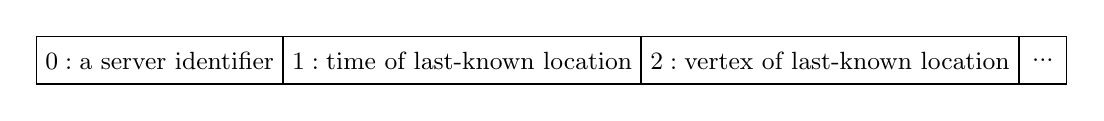
\begin{tikzpicture}
\small
\matrix[nodes={draw,minimum size=6mm}] {
  \node {$0:\textrm{a server identifier}$};
 &\node {$1:\textrm{time of last-known location}$};
 &\node {$2:\textrm{vertex of last-known location}$};
 &\node {...};\\
};
\end{tikzpicture}\\
\textbf{Side Effects:} none.\\
\textbf{Throws:} {\tt{}SQLException} if database failure is encountered.\\
\bottomrule
\end{tabular}
\nwenddocs{}\nwbegincode{133}\sublabel{NW18ZcDF-1zUdrf-1}\nwmargintag{{\nwtagstyle{}\subpageref{NW18ZcDF-1zUdrf-1}}}\moddef{Read: DBQueryServersLocations(1)~{\nwtagstyle{}\subpageref{NW18ZcDF-1zUdrf-1}}}\endmoddef\nwused{\\{NW3x1zuR-Oyob-1}}
int[] DBQueryServersLocations(final int t) throws SQLException \{
  try (\LA{}Open \code{}conn\edoc{}~{\nwtagstyle{}\subpageref{NWgUSr6-JT1v9-1}}\RA{}) \{
    return this.PSQuery(conn, "S59", 3, t, t, t, t);
  \} catch (SQLException e) \{
    throw e;
  \}
\}
\nwindexdefn{DBQueryServersLocations}{DBQueryServersLocations}{NW18ZcDF-1zUdrf-1}\eatline
\nwidentdefs{\\{{DBQueryServersLocations}{DBQueryServersLocations}}}\nwidentuses{\\{{PSQuery}{PSQuery}}\\{{S59}{S59}}}\nwindexuse{PSQuery}{PSQuery}{NW18ZcDF-1zUdrf-1}\nwindexuse{S59}{S59}{NW18ZcDF-1zUdrf-1}\nwendcode{}\nwbegindocs{134}\nwdocspar
\subsection{\texttt{DBQueryServersLocationsActive}(1)}
\begin{tabular}{p{\textwidth}}
\toprule
\rowcolor{TableTitle}
SINGLE-THREAD ONLY. Method \textcolor{blue}{{\tt{}\protect\nwindexuse{DBQueryServersLocationsActive}{DBQueryServersLocationsActive}{NW18ZcDF-2tWQc-1}DBQueryServersLocationsActive}}(1) returns the
last-known locations of all active servers at the given time. A server is
``active'' if its service has not ended, in other words it has not arrived
at its own destination.
The ``last-known location'' is the waypoint in the server's route $w$
with a time component closest to but not exceeding the given time, in other
words ${w_{\leq t}}_{|w_{\leq t}|}$.
A {\tt{}SQLException} is thrown in case of database failure.\\
\midrule
\textbf{Parameters:} \\
\begin{tabular}{lp{116mm}}
Integer {\tt{}t} (param. 1):&a time
\end{tabular}\\
\textbf{Returns:} results of the query flattened into an integer array, or
{\tt{}null} if no results.

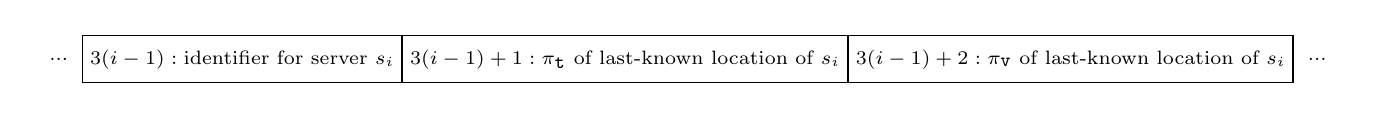
\begin{tikzpicture}
\scriptsize
\matrix[nodes={minimum size=6mm}] {
  \node {...};
 &\node[draw] {$3(i-1):\textrm{identifier for server $s_i$}$};
 &\node[draw] {$3(i-1)+1:\pi_\texttt{t}\textrm{ of last-known location of $s_i$}$};
 &\node[draw] {$3(i-1)+2:\pi_\texttt{v}\textrm{ of last-known location of $s_i$}$};
 &\node {...};\\
};
\end{tikzpicture}\\

where $1\leq i\leq |\mathcal{S}^\textrm{active}|$,
$s_i\in \mathcal{S}^\textrm{active}$, and
$\mathcal{S}^\textrm{active}= \{s\in\mathcal{S}\mid t^\textrm{arrive}(\mathcal{X},s)>t\}|$
for $t$ given by param. 1.\\
\textbf{Side Effects:} none.\\
\textbf{Throws:} {\tt{}SQLException} if database failure is encountered.\\
\bottomrule
\end{tabular}
\nwenddocs{}\nwbegincode{135}\sublabel{NW18ZcDF-2tWQc-1}\nwmargintag{{\nwtagstyle{}\subpageref{NW18ZcDF-2tWQc-1}}}\moddef{Read: DBQueryServersLocationsActive(1)~{\nwtagstyle{}\subpageref{NW18ZcDF-2tWQc-1}}}\endmoddef\nwalsodefined{\\{NW18ZcDF-2tWQc-2}}\nwused{\\{NW3x1zuR-Oyob-1}}
int[] DBQueryServersLocationsActive(final int t) throws SQLException \{
  int[] output = new int[] \{ \};
  try (\LA{}Open \code{}conn\edoc{}~{\nwtagstyle{}\subpageref{NWgUSr6-JT1v9-1}}\RA{}) \{
    int j = 0;
\nosublabel{NW18ZcDF-2tWQc-1-u1}\nwindexdefn{DBQueryServersLocationsActive}{DBQueryServersLocationsActive}{NW18ZcDF-2tWQc-1}\eatline
\nwidentdefs{\\{{DBQueryServersLocationsActive}{DBQueryServersLocationsActive}}}\nwendcode{}\nwbegindocs{136}{\small Our approach is to first use statement {\tt{}\protect\nwindexuse{S134}{S134}{NWgUSr6-9eEGJ-1}S134} to get the active
servers. Then for each active server, we use either statement {\tt{}\protect\nwindexuse{S135}{S135}{NWgUSr6-4dp7jX-1}S135} or
{\tt{}\protect\nwindexuse{S147}{S147}{NWgUSr6-2TcddD-1}S147} to get its last-known location.}
\nwenddocs{}\nwbegincode{137}\sublabel{NW18ZcDF-2tWQc-2}\nwmargintag{{\nwtagstyle{}\subpageref{NW18ZcDF-2tWQc-2}}}\moddef{Read: DBQueryServersLocationsActive(1)~{\nwtagstyle{}\subpageref{NW18ZcDF-2tWQc-1}}}\plusendmoddef
    // Query S134 selects from CW. The query time is not expected to grow
    // because Table CW does not grow as we pre-load all the servers when we
    // load the problem instance.
    final int[] temp1 = this.PSQuery(conn, "S134", 2, t, t, t);  // <-- 10 ms/call
    output = new int[(3*(temp1.length/2))];
    for (int i = 0; i < temp1.length - 1; i += 2) \{
      final int sid = temp1[(i + 0)];
      final int  te = temp1[(i + 1)];
      // Query S135 selects from W. The query time is expected to grow
      // O(log(|W|)) because we have indexes on the relevant columns,
      // implemented in Derby as B+trees (https://db.apache.org/derby/papers/btree_package.html).
      // The subquery in S135 is a range query with a tight range.
      // Query S147 is a key-lookup and also grows O(log(|W|)).
      final int lvt = this.lu_lvt.get(sid);
      final int[] temp2 = (t < te
        ? this.PSQuery(conn, "S135", 2, sid, sid, lvt, t, t)
        : this.PSQuery(conn, "S147", 2, sid, sid));
      output[(j + 0)] = sid;
      output[(j + 1)] = temp2[0];
      output[(j + 2)] = temp2[1];
      this.lu_lvt.put(sid, temp2[0]);
      j += 3;
    \}
  \} catch (SQLException e) \{
    throw e;
  \}
  return output;
\}
\nwidentuses{\\{{PSQuery}{PSQuery}}\\{{query}{query}}\\{{S134}{S134}}\\{{S135}{S135}}\\{{S147}{S147}}}\nwindexuse{PSQuery}{PSQuery}{NW18ZcDF-2tWQc-2}\nwindexuse{query}{query}{NW18ZcDF-2tWQc-2}\nwindexuse{S134}{S134}{NW18ZcDF-2tWQc-2}\nwindexuse{S135}{S135}{NW18ZcDF-2tWQc-2}\nwindexuse{S147}{S147}{NW18ZcDF-2tWQc-2}\nwendcode{}\nwbegindocs{138}\nwdocspar
\begin{tabular}{p{\textwidth}}
\toprule
\rowcolor{TableTitle}
Method \textcolor{blue}{{\tt{}\protect\nwindexuse{queryServersLocationsActive}{queryServersLocationsActive}{NW18ZcDF-t5O2a-1}queryServersLocationsActive}}(1) wraps {\tt{}\protect\nwindexuse{DBQueryServersLocationsActive}{DBQueryServersLocationsActive}{NW18ZcDF-2tWQc-1}DBQueryServersLocationsActive}(1).\\
\bottomrule
\end{tabular}
\nwenddocs{}\nwbegincode{139}\sublabel{NW18ZcDF-t5O2a-1}\nwmargintag{{\nwtagstyle{}\subpageref{NW18ZcDF-t5O2a-1}}}\moddef{Read: queryServersLocationsActive(1)~{\nwtagstyle{}\subpageref{NW18ZcDF-t5O2a-1}}}\endmoddef\nwused{\\{NW3x1zuR-2Rlctf-1}}
int[] queryServersLocationsActive(final int t) throws SQLException \{
  long A0 = System.currentTimeMillis();
  int[] output = this.storage.DBQueryServersLocationsActive(t);
  \LA{}Stats: queryServersLocationsActive~{\nwtagstyle{}\subpageref{NW1n2CZQ-3FW4vm-1}}\RA{}
  return output;
\}
\nosublabel{NW18ZcDF-t5O2a-1-u1}\nwindexdefn{queryServersLocationsActive}{queryServersLocationsActive}{NW18ZcDF-t5O2a-1}\eatline
\nwidentdefs{\\{{queryServersLocationsActive}{queryServersLocationsActive}}}\nwidentuses{\\{{DBQueryServersLocationsActive}{DBQueryServersLocationsActive}}}\nwindexuse{DBQueryServersLocationsActive}{DBQueryServersLocationsActive}{NW18ZcDF-t5O2a-1}\nwendcode{}\nwbegindocs{140}\nwdocspar
\section{Methods: Read Metrics}

\subsection{\texttt{DBQueryMetricServiceRate}(0)}
\begin{tabular}{p{\textwidth}}
\toprule
\rowcolor{TableTitle}
Method \textcolor{blue}{{\tt{}\protect\nwindexuse{DBQueryMetricServiceRate}{DBQueryMetricServiceRate}{NW18ZcDF-49bCCM-1}DBQueryMetricServiceRate}}(0) returns the
service rate $\mu$ (Eq.~\ref{eq:service-rate}).
A {\tt{}SQLException} is thrown in case of database failure.\\
\midrule
\textbf{Parameters:} none.\\
\textbf{Returns:} results of the query flattened into an integer array,
or {\tt{}null} if no results.

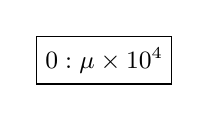
\begin{tikzpicture}
\small
\matrix[nodes={minimum size=6mm}] {
  \node[draw] {$0:\mu\times 10^4$};\\
};
\end{tikzpicture}

Note that the service rate is \textbf{multiplied by $10^4$} so that it can be
returned as an integer with 2 decimal points precision, for example if
$\mu=.1234$, then {\tt{}\protect\nwindexuse{DBQueryMetricServiceRate}{DBQueryMetricServiceRate}{NW18ZcDF-49bCCM-1}DBQueryMetricServiceRate}(0) returns $1234$.\\
\textbf{Side Effects:} none.\\
\textbf{Throws:} {\tt{}SQLException} if database failure is encountered.\\
\bottomrule
\end{tabular}
\nwenddocs{}\nwbegincode{141}\sublabel{NW18ZcDF-49bCCM-1}\nwmargintag{{\nwtagstyle{}\subpageref{NW18ZcDF-49bCCM-1}}}\moddef{Read: DBQueryMetricServiceRate(0)~{\nwtagstyle{}\subpageref{NW18ZcDF-49bCCM-1}}}\endmoddef\nwused{\\{NW3x1zuR-Oyob-1}}
int[] DBQueryMetricServiceRate() throws SQLException \{
  try (\LA{}Open \code{}conn\edoc{}~{\nwtagstyle{}\subpageref{NWgUSr6-JT1v9-1}}\RA{}) \{
    return PSQuery(conn, "S102", 1);
  \} catch (SQLException e) \{
    throw e;
  \}
\}
\nwindexdefn{DBQueryMetricServiceRate}{DBQueryMetricServiceRate}{NW18ZcDF-49bCCM-1}\eatline
\nwidentdefs{\\{{DBQueryMetricServiceRate}{DBQueryMetricServiceRate}}}\nwidentuses{\\{{PSQuery}{PSQuery}}\\{{S102}{S102}}}\nwindexuse{PSQuery}{PSQuery}{NW18ZcDF-49bCCM-1}\nwindexuse{S102}{S102}{NW18ZcDF-49bCCM-1}\nwendcode{}\nwbegindocs{142}\begin{tabular}{p{\textwidth}}
\toprule
\rowcolor{TableTitle}
Method \textcolor{blue}{{\tt{}\protect\nwindexuse{queryMetricServiceRate}{queryMetricServiceRate}{NW18ZcDF-f55U7-1}queryMetricServiceRate}}(0) wraps {\tt{}\protect\nwindexuse{DBQueryMetricServiceRate}{DBQueryMetricServiceRate}{NW18ZcDF-49bCCM-1}DBQueryMetricServiceRate}(0).\\
\bottomrule
\end{tabular}
\nwenddocs{}\nwbegincode{143}\sublabel{NW18ZcDF-f55U7-1}\nwmargintag{{\nwtagstyle{}\subpageref{NW18ZcDF-f55U7-1}}}\moddef{Read: queryMetricServiceRate(0)~{\nwtagstyle{}\subpageref{NW18ZcDF-f55U7-1}}}\endmoddef\nwused{\\{NW3x1zuR-2u8vSA-1}}
int[] queryMetricServiceRate() throws SQLException \{
  return storage.DBQueryMetricServiceRate();
\}
\nwindexdefn{queryMetricServiceRate}{queryMetricServiceRate}{NW18ZcDF-f55U7-1}\eatline
\nwidentdefs{\\{{queryMetricServiceRate}{queryMetricServiceRate}}}\nwidentuses{\\{{DBQueryMetricServiceRate}{DBQueryMetricServiceRate}}}\nwindexuse{DBQueryMetricServiceRate}{DBQueryMetricServiceRate}{NW18ZcDF-f55U7-1}\nwendcode{}\nwbegindocs{144}\nwdocspar
\subsection{\texttt{DBQueryMetricUserDistanceBaseTotal}(0)}
\begin{tabular}{p{\textwidth}}
\toprule
\rowcolor{TableTitle}
Method \textcolor{blue}{{\tt{}\protect\nwindexuse{DBQueryMetricUserDistanceBaseTotal}{DBQueryMetricUserDistanceBaseTotal}{NW18ZcDF-1ZAnmM-1}DBQueryMetricUserDistanceBaseTotal}}(0) returns the
base distance $D^\textrm{base}(\mathcal{U})$ (Eq.~\ref{eq:base-distance}).
A {\tt{}SQLException} is thrown in case of database failure.\\
\midrule
\textbf{Parameters:} none.\\
\textbf{Returns:} results of the query flattened into an integer array,
or {\tt{}null} if no results.

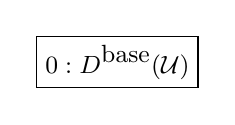
\begin{tikzpicture}
\small
\matrix[nodes={minimum size=6mm}] {
  \node[draw] {$0:D^\textrm{base}(\mathcal{U})$};\\
};
\end{tikzpicture}\\
\textbf{Side Effects:} none.\\
\textbf{Throws:} {\tt{}SQLException} if database failure is encountered.\\
\bottomrule
\end{tabular}
\nwenddocs{}\nwbegincode{145}\sublabel{NW18ZcDF-1ZAnmM-1}\nwmargintag{{\nwtagstyle{}\subpageref{NW18ZcDF-1ZAnmM-1}}}\moddef{Read: DBQueryMetricUserDistanceBaseTotal(0)~{\nwtagstyle{}\subpageref{NW18ZcDF-1ZAnmM-1}}}\endmoddef\nwused{\\{NW3x1zuR-Oyob-1}}
int[] DBQueryMetricUserDistanceBaseTotal() throws SQLException \{
  try (\LA{}Open \code{}conn\edoc{}~{\nwtagstyle{}\subpageref{NWgUSr6-JT1v9-1}}\RA{}) \{
    return PSQuery(conn, "S103", 1);
  \} catch (SQLException e) \{
    throw e;
  \}
\}
\nwindexdefn{DBQueryMetricUserDistanceBaseTotal}{DBQueryMetricUserDistanceBaseTotal}{NW18ZcDF-1ZAnmM-1}\eatline
\nwidentdefs{\\{{DBQueryMetricUserDistanceBaseTotal}{DBQueryMetricUserDistanceBaseTotal}}}\nwidentuses{\\{{PSQuery}{PSQuery}}\\{{S103}{S103}}}\nwindexuse{PSQuery}{PSQuery}{NW18ZcDF-1ZAnmM-1}\nwindexuse{S103}{S103}{NW18ZcDF-1ZAnmM-1}\nwendcode{}\nwbegindocs{146}\begin{tabular}{p{\textwidth}}
\toprule
\rowcolor{TableTitle}
Method \textcolor{blue}{{\tt{}\protect\nwindexuse{queryMetricUserDistanceBaseTotal}{queryMetricUserDistanceBaseTotal}{NW18ZcDF-4C6HwO-1}queryMetricUserDistanceBaseTotal}}(0) wraps {\tt{}\protect\nwindexuse{DBQueryMetricUserDistanceBaseTotal}{DBQueryMetricUserDistanceBaseTotal}{NW18ZcDF-1ZAnmM-1}DBQueryMetricUserDistanceBaseTotal}(0).\\
\bottomrule
\end{tabular}
\nwenddocs{}\nwbegincode{147}\sublabel{NW18ZcDF-4C6HwO-1}\nwmargintag{{\nwtagstyle{}\subpageref{NW18ZcDF-4C6HwO-1}}}\moddef{Read: queryMetricUserDistanceBaseTotal(0)~{\nwtagstyle{}\subpageref{NW18ZcDF-4C6HwO-1}}}\endmoddef\nwused{\\{NW3x1zuR-2u8vSA-1}}
int[] queryMetricUserDistanceBaseTotal() throws SQLException \{
  return storage.DBQueryMetricUserDistanceBaseTotal();
\}
\nwindexdefn{queryMetricUserDistanceBaseTotal}{queryMetricUserDistanceBaseTotal}{NW18ZcDF-4C6HwO-1}\eatline
\nwidentdefs{\\{{queryMetricUserDistanceBaseTotal}{queryMetricUserDistanceBaseTotal}}}\nwidentuses{\\{{DBQueryMetricUserDistanceBaseTotal}{DBQueryMetricUserDistanceBaseTotal}}}\nwindexuse{DBQueryMetricUserDistanceBaseTotal}{DBQueryMetricUserDistanceBaseTotal}{NW18ZcDF-4C6HwO-1}\nwendcode{}\nwbegindocs{148}\nwdocspar
\subsection{\texttt{DBQueryMetricServerDistanceTotal}(0)}
\begin{tabular}{p{\textwidth}}
\toprule
\rowcolor{TableTitle}
Method \textcolor{blue}{{\tt{}\protect\nwindexuse{DBQueryMetricServerDistanceTotal}{DBQueryMetricServerDistanceTotal}{NW18ZcDF-47NowU-1}DBQueryMetricServerDistanceTotal}}(0) returns the
total travel distance of all the servers.
A {\tt{}SQLException} is thrown in case of database failure.\\
\midrule
\textbf{Parameters:} none.\\
\textbf{Returns:} results of the query flattened into an integer array,
or {\tt{}null} if no results.

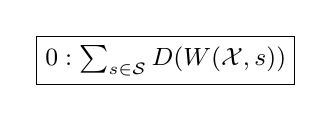
\begin{tikzpicture}
\small
\matrix[nodes={minimum size=6mm}] {
  \node[draw] {$0:\sum_{s\in\mathcal{S}}D(W(\mathcal{X},s))$};\\
};
\end{tikzpicture}\\
\textbf{Side Effects:} none.\\
\textbf{Throws:} {\tt{}SQLException} if database failure is encountered.\\
\bottomrule
\end{tabular}
\nwenddocs{}\nwbegincode{149}\sublabel{NW18ZcDF-47NowU-1}\nwmargintag{{\nwtagstyle{}\subpageref{NW18ZcDF-47NowU-1}}}\moddef{Read: DBQueryMetricServerDistanceTotal(0)~{\nwtagstyle{}\subpageref{NW18ZcDF-47NowU-1}}}\endmoddef\nwused{\\{NW3x1zuR-Oyob-1}}
int[] DBQueryMetricServerDistanceTotal() throws SQLException \{
  try (\LA{}Open \code{}conn\edoc{}~{\nwtagstyle{}\subpageref{NWgUSr6-JT1v9-1}}\RA{}) \{
    return PSQuery(conn, "S105", 1);
  \} catch (SQLException e) \{
    throw e;
  \}
\}
\nwindexdefn{DBQueryMetricServerDistanceTotal}{DBQueryMetricServerDistanceTotal}{NW18ZcDF-47NowU-1}\eatline
\nwidentdefs{\\{{DBQueryMetricServerDistanceTotal}{DBQueryMetricServerDistanceTotal}}}\nwidentuses{\\{{PSQuery}{PSQuery}}\\{{S105}{S105}}}\nwindexuse{PSQuery}{PSQuery}{NW18ZcDF-47NowU-1}\nwindexuse{S105}{S105}{NW18ZcDF-47NowU-1}\nwendcode{}\nwbegindocs{150}\begin{tabular}{p{\textwidth}}
\toprule
\rowcolor{TableTitle}
Method \textcolor{blue}{{\tt{}\protect\nwindexuse{queryMetricServerDistanceTotal}{queryMetricServerDistanceTotal}{NW18ZcDF-4fAqgC-1}queryMetricServerDistanceTotal}}(0) wraps {\tt{}\protect\nwindexuse{DBQueryMetricServerDistanceTotal}{DBQueryMetricServerDistanceTotal}{NW18ZcDF-47NowU-1}DBQueryMetricServerDistanceTotal}(0).\\
\bottomrule
\end{tabular}
\nwenddocs{}\nwbegincode{151}\sublabel{NW18ZcDF-4fAqgC-1}\nwmargintag{{\nwtagstyle{}\subpageref{NW18ZcDF-4fAqgC-1}}}\moddef{Read: queryMetricServerDistanceTotal(0)~{\nwtagstyle{}\subpageref{NW18ZcDF-4fAqgC-1}}}\endmoddef\nwused{\\{NW3x1zuR-2u8vSA-1}}
int[] queryMetricServerDistanceTotal() throws SQLException \{
  return storage.DBQueryMetricServerDistanceTotal();
\}
\nwindexdefn{queryMetricServerDistanceTotal}{queryMetricServerDistanceTotal}{NW18ZcDF-4fAqgC-1}\eatline
\nwidentdefs{\\{{queryMetricServerDistanceTotal}{queryMetricServerDistanceTotal}}}\nwidentuses{\\{{DBQueryMetricServerDistanceTotal}{DBQueryMetricServerDistanceTotal}}}\nwindexuse{DBQueryMetricServerDistanceTotal}{DBQueryMetricServerDistanceTotal}{NW18ZcDF-4fAqgC-1}\nwendcode{}\nwbegindocs{152}\nwdocspar
\subsection{\texttt{DBQueryMetricServerDistanceBaseTotal}(0)}
\begin{tabular}{p{\textwidth}}
\toprule
\rowcolor{TableTitle}
Method \textcolor{blue}{{\tt{}\protect\nwindexuse{DBQueryMetricServerDistanceBaseTotal}{DBQueryMetricServerDistanceBaseTotal}{NW18ZcDF-2gaNGt-1}DBQueryMetricServerDistanceBaseTotal}}(0) returns the
base distance of all the servers.
A {\tt{}SQLException} is thrown in case of database failure.\\
\midrule
\textbf{Parameters:} none.\\
\textbf{Returns:} results of the query flattened into an integer array,
or {\tt{}null} if no results.

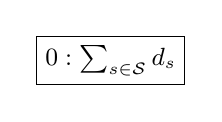
\begin{tikzpicture}
\small
\matrix[nodes={minimum size=6mm}] {
  \node[draw] {$0:\sum_{s\in\mathcal{S}}d_s$};\\
};
\end{tikzpicture}\\
\textbf{Side Effects:} none.\\
\textbf{Throws:} {\tt{}SQLException} if database failure is encountered.\\
\bottomrule
\end{tabular}
\nwenddocs{}\nwbegincode{153}\sublabel{NW18ZcDF-2gaNGt-1}\nwmargintag{{\nwtagstyle{}\subpageref{NW18ZcDF-2gaNGt-1}}}\moddef{Read: DBQueryMetricServerDistanceBaseTotal(0)~{\nwtagstyle{}\subpageref{NW18ZcDF-2gaNGt-1}}}\endmoddef\nwused{\\{NW3x1zuR-Oyob-1}}
int[] DBQueryMetricServerDistanceBaseTotal() throws SQLException \{
  try (\LA{}Open \code{}conn\edoc{}~{\nwtagstyle{}\subpageref{NWgUSr6-JT1v9-1}}\RA{}) \{
    return PSQuery(conn, "S110", 1);
  \} catch (SQLException e) \{
    throw e;
  \}
\}
\nwindexdefn{DBQueryMetricServerDistanceBaseTotal}{DBQueryMetricServerDistanceBaseTotal}{NW18ZcDF-2gaNGt-1}\eatline
\nwidentdefs{\\{{DBQueryMetricServerDistanceBaseTotal}{DBQueryMetricServerDistanceBaseTotal}}}\nwidentuses{\\{{PSQuery}{PSQuery}}\\{{S110}{S110}}}\nwindexuse{PSQuery}{PSQuery}{NW18ZcDF-2gaNGt-1}\nwindexuse{S110}{S110}{NW18ZcDF-2gaNGt-1}\nwendcode{}\nwbegindocs{154}\begin{tabular}{p{\textwidth}}
\toprule
\rowcolor{TableTitle}
Method \textcolor{blue}{{\tt{}\protect\nwindexuse{queryMetricServerDistanceBaseTotal}{queryMetricServerDistanceBaseTotal}{NW18ZcDF-2ZOFmc-1}queryMetricServerDistanceBaseTotal}}(0) wraps {\tt{}\protect\nwindexuse{DBQueryMetricServerDistanceBaseTotal}{DBQueryMetricServerDistanceBaseTotal}{NW18ZcDF-2gaNGt-1}DBQueryMetricServerDistanceBaseTotal}(0).\\
\bottomrule
\end{tabular}
\nwenddocs{}\nwbegincode{155}\sublabel{NW18ZcDF-2ZOFmc-1}\nwmargintag{{\nwtagstyle{}\subpageref{NW18ZcDF-2ZOFmc-1}}}\moddef{Read: queryMetricServerDistanceBaseTotal(0)~{\nwtagstyle{}\subpageref{NW18ZcDF-2ZOFmc-1}}}\endmoddef\nwused{\\{NW3x1zuR-2u8vSA-1}}
int[] queryMetricServerDistanceBaseTotal() throws SQLException \{
  return storage.DBQueryMetricServerDistanceBaseTotal();
\}
\nwindexdefn{queryMetricServerDistanceBaseTotal}{queryMetricServerDistanceBaseTotal}{NW18ZcDF-2ZOFmc-1}\eatline
\nwidentdefs{\\{{queryMetricServerDistanceBaseTotal}{queryMetricServerDistanceBaseTotal}}}\nwidentuses{\\{{DBQueryMetricServerDistanceBaseTotal}{DBQueryMetricServerDistanceBaseTotal}}}\nwindexuse{DBQueryMetricServerDistanceBaseTotal}{DBQueryMetricServerDistanceBaseTotal}{NW18ZcDF-2ZOFmc-1}\nwendcode{}\nwbegindocs{156}\nwdocspar
\subsection{\texttt{DBQueryMetricServerDistanceCruisingTotal}(0)}
\begin{tabular}{p{\textwidth}}
\toprule
\rowcolor{TableTitle}
Method \textcolor{blue}{{\tt{}\protect\nwindexuse{DBQueryMetricServerDistanceCruisingTotal}{DBQueryMetricServerDistanceCruisingTotal}{NW18ZcDF-3ENmOe-1}DBQueryMetricServerDistanceCruisingTotal}}(0) returns the
total cruising distance of all servers.
A {\tt{}SQLException} is thrown in case of database failure.\\
\midrule
\textbf{Parameters:} none.\\
\textbf{Returns:} results of the query flattened into an integer array,
or {\tt{}null} if no results.

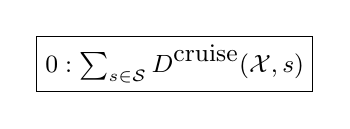
\begin{tikzpicture}
\small
\matrix[nodes={minimum size=6mm}] {
  \node[draw] {$0:\sum_{s\in\mathcal{S}}D^\textrm{cruise}(\mathcal{X},s)$};\\
};
\end{tikzpicture}\\
\textbf{Side Effects:} none.\\
\textbf{Throws:} {\tt{}SQLException} if database failure is encountered.\\
\bottomrule
\end{tabular}
\nwenddocs{}\nwbegincode{157}\sublabel{NW18ZcDF-3ENmOe-1}\nwmargintag{{\nwtagstyle{}\subpageref{NW18ZcDF-3ENmOe-1}}}\moddef{Read: DBQueryMetricServerDistanceCruisingTotal(0)~{\nwtagstyle{}\subpageref{NW18ZcDF-3ENmOe-1}}}\endmoddef\nwused{\\{NW3x1zuR-Oyob-1}}
int[] DBQueryMetricServerDistanceCruisingTotal() throws SQLException \{
  try (\LA{}Open \code{}conn\edoc{}~{\nwtagstyle{}\subpageref{NWgUSr6-JT1v9-1}}\RA{}) \{
    return PSQuery(conn, "S107", 1);
  \} catch (SQLException e) \{
    throw e;
  \}
\}
\nwindexdefn{DBQueryMetricServerDistanceCruisingTotal}{DBQueryMetricServerDistanceCruisingTotal}{NW18ZcDF-3ENmOe-1}\eatline
\nwidentdefs{\\{{DBQueryMetricServerDistanceCruisingTotal}{DBQueryMetricServerDistanceCruisingTotal}}}\nwidentuses{\\{{PSQuery}{PSQuery}}\\{{S107}{S107}}}\nwindexuse{PSQuery}{PSQuery}{NW18ZcDF-3ENmOe-1}\nwindexuse{S107}{S107}{NW18ZcDF-3ENmOe-1}\nwendcode{}\nwbegindocs{158}\begin{tabular}{p{\textwidth}}
\toprule
\rowcolor{TableTitle}
Method \textcolor{blue}{{\tt{}\protect\nwindexuse{queryMetricServerDistanceCruisingTotal}{queryMetricServerDistanceCruisingTotal}{NW18ZcDF-2TPHRC-1}queryMetricServerDistanceCruisingTotal}}(0) wraps {\tt{}\protect\nwindexuse{DBQueryMetricServerDistanceCruisingTotal}{DBQueryMetricServerDistanceCruisingTotal}{NW18ZcDF-3ENmOe-1}DBQueryMetricServerDistanceCruisingTotal}(0).\\
\bottomrule
\end{tabular}
\nwenddocs{}\nwbegincode{159}\sublabel{NW18ZcDF-2TPHRC-1}\nwmargintag{{\nwtagstyle{}\subpageref{NW18ZcDF-2TPHRC-1}}}\moddef{Read: queryMetricServerDistanceCruisingTotal(0)~{\nwtagstyle{}\subpageref{NW18ZcDF-2TPHRC-1}}}\endmoddef\nwused{\\{NW3x1zuR-2u8vSA-1}}
int[] queryMetricServerDistanceCruisingTotal() throws SQLException \{
  return storage.DBQueryMetricServerDistanceCruisingTotal();
\}
\nwindexdefn{queryMetricServerDistanceCruisingTotal}{queryMetricServerDistanceCruisingTotal}{NW18ZcDF-2TPHRC-1}\eatline
\nwidentdefs{\\{{queryMetricServerDistanceCruisingTotal}{queryMetricServerDistanceCruisingTotal}}}\nwidentuses{\\{{DBQueryMetricServerDistanceCruisingTotal}{DBQueryMetricServerDistanceCruisingTotal}}}\nwindexuse{DBQueryMetricServerDistanceCruisingTotal}{DBQueryMetricServerDistanceCruisingTotal}{NW18ZcDF-2TPHRC-1}\nwendcode{}\nwbegindocs{160}\nwdocspar
\subsection{\texttt{DBQueryMetricServerDistanceServiceTotal}(0)}
\begin{tabular}{p{\textwidth}}
\toprule
\rowcolor{TableTitle}
Method \textcolor{blue}{{\tt{}\protect\nwindexuse{DBQueryMetricServerDistanceServiceTotal}{DBQueryMetricServerDistanceServiceTotal}{NW18ZcDF-423lHf-1}DBQueryMetricServerDistanceServiceTotal}}(0) returns the
total service distance of all servers.
A {\tt{}SQLException} is thrown in case of database failure.\\
\midrule
\textbf{Parameters:} none.\\
\textbf{Returns:} results of the query flattened into an integer array,
or {\tt{}null} if no results.

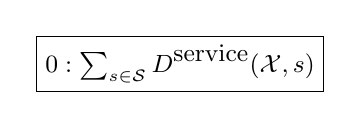
\begin{tikzpicture}
\small
\matrix[nodes={minimum size=6mm}] {
  \node[draw] {$0:\sum_{s\in\mathcal{S}}D^\textrm{service}(\mathcal{X},s)$};\\
};
\end{tikzpicture}\\
\textbf{Side Effects:} none.\\
\textbf{Throws:} {\tt{}SQLException} if database failure is encountered.\\
\bottomrule
\end{tabular}
\nwenddocs{}\nwbegincode{161}\sublabel{NW18ZcDF-423lHf-1}\nwmargintag{{\nwtagstyle{}\subpageref{NW18ZcDF-423lHf-1}}}\moddef{Read: DBQueryMetricServerDistanceServiceTotal(0)~{\nwtagstyle{}\subpageref{NW18ZcDF-423lHf-1}}}\endmoddef\nwused{\\{NW3x1zuR-Oyob-1}}
int[] DBQueryMetricServerDistanceServiceTotal() throws SQLException \{
  try (\LA{}Open \code{}conn\edoc{}~{\nwtagstyle{}\subpageref{NWgUSr6-JT1v9-1}}\RA{}) \{
    return PSQuery(conn, "S109", 1);
  \} catch (SQLException e) \{
    throw e;
  \}
\}
\nwindexdefn{DBQueryMetricServerDistanceServiceTotal}{DBQueryMetricServerDistanceServiceTotal}{NW18ZcDF-423lHf-1}\eatline
\nwidentdefs{\\{{DBQueryMetricServerDistanceServiceTotal}{DBQueryMetricServerDistanceServiceTotal}}}\nwidentuses{\\{{PSQuery}{PSQuery}}\\{{S109}{S109}}}\nwindexuse{PSQuery}{PSQuery}{NW18ZcDF-423lHf-1}\nwindexuse{S109}{S109}{NW18ZcDF-423lHf-1}\nwendcode{}\nwbegindocs{162}\begin{tabular}{p{\textwidth}}
\toprule
\rowcolor{TableTitle}
Method \textcolor{blue}{{\tt{}\protect\nwindexuse{queryMetricServerDistanceServiceTotal}{queryMetricServerDistanceServiceTotal}{NW18ZcDF-14khfr-1}queryMetricServerDistanceServiceTotal}}(0) wraps {\tt{}\protect\nwindexuse{DBQueryMetricServerDistanceServiceTotal}{DBQueryMetricServerDistanceServiceTotal}{NW18ZcDF-423lHf-1}DBQueryMetricServerDistanceServiceTotal}(0).\\
\bottomrule
\end{tabular}
\nwenddocs{}\nwbegincode{163}\sublabel{NW18ZcDF-14khfr-1}\nwmargintag{{\nwtagstyle{}\subpageref{NW18ZcDF-14khfr-1}}}\moddef{Read: queryMetricServerDistanceServiceTotal(0)~{\nwtagstyle{}\subpageref{NW18ZcDF-14khfr-1}}}\endmoddef\nwused{\\{NW3x1zuR-2u8vSA-1}}
int[] queryMetricServerDistanceServiceTotal() throws SQLException \{
  return storage.DBQueryMetricServerDistanceServiceTotal();
\}
\nwindexdefn{queryMetricServerDistanceServiceTotal}{queryMetricServerDistanceServiceTotal}{NW18ZcDF-14khfr-1}\eatline
\nwidentdefs{\\{{queryMetricServerDistanceServiceTotal}{queryMetricServerDistanceServiceTotal}}}\nwidentuses{\\{{DBQueryMetricServerDistanceServiceTotal}{DBQueryMetricServerDistanceServiceTotal}}}\nwindexuse{DBQueryMetricServerDistanceServiceTotal}{DBQueryMetricServerDistanceServiceTotal}{NW18ZcDF-14khfr-1}\nwendcode{}\nwbegindocs{164}\nwdocspar
\subsection{\texttt{DBQueryMetricServerDurationTravelTotal}(0)}
\begin{tabular}{p{\textwidth}}
\toprule
\rowcolor{TableTitle}
Method \textcolor{blue}{{\tt{}\protect\nwindexuse{DBQueryMetricServerDurationTravelTotal}{DBQueryMetricServerDurationTravelTotal}{NW18ZcDF-4UAOce-1}DBQueryMetricServerDurationTravelTotal}}(0) returns the
total travel duration of all servers.
A {\tt{}SQLException} is thrown in case of database failure.\\
\midrule
\textbf{Parameters:} none.\\
\textbf{Returns:} results of the query flattened into an integer array,
or {\tt{}null} if no results.

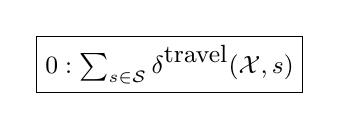
\begin{tikzpicture}
\small
\matrix[nodes={minimum size=6mm}] {
  \node[draw] {$0:\sum_{s\in\mathcal{S}}\delta^\textrm{travel}(\mathcal{X},s)$};\\
};
\end{tikzpicture}\\
\textbf{Side Effects:} none.\\
\textbf{Throws:} {\tt{}SQLException} if database failure is encountered.\\
\bottomrule
\end{tabular}
\nwenddocs{}\nwbegincode{165}\sublabel{NW18ZcDF-4UAOce-1}\nwmargintag{{\nwtagstyle{}\subpageref{NW18ZcDF-4UAOce-1}}}\moddef{Read: DBQueryMetricServerDurationTravelTotal(0)~{\nwtagstyle{}\subpageref{NW18ZcDF-4UAOce-1}}}\endmoddef\nwused{\\{NW3x1zuR-Oyob-1}}
int[] DBQueryMetricServerDurationTravelTotal() throws SQLException \{
  try (\LA{}Open \code{}conn\edoc{}~{\nwtagstyle{}\subpageref{NWgUSr6-JT1v9-1}}\RA{}) \{
    return PSQuery(conn, "S117", 1);
  \} catch (SQLException e) \{
    throw e;
  \}
\}
\nwindexdefn{DBQueryMetricServerDurationTravelTotal}{DBQueryMetricServerDurationTravelTotal}{NW18ZcDF-4UAOce-1}\eatline
\nwidentdefs{\\{{DBQueryMetricServerDurationTravelTotal}{DBQueryMetricServerDurationTravelTotal}}}\nwidentuses{\\{{PSQuery}{PSQuery}}\\{{S117}{S117}}}\nwindexuse{PSQuery}{PSQuery}{NW18ZcDF-4UAOce-1}\nwindexuse{S117}{S117}{NW18ZcDF-4UAOce-1}\nwendcode{}\nwbegindocs{166}\begin{tabular}{p{\textwidth}}
\toprule
\rowcolor{TableTitle}
Method \textcolor{blue}{{\tt{}\protect\nwindexuse{queryMetricServerDurationTravelTotal}{queryMetricServerDurationTravelTotal}{NW18ZcDF-3kbNxN-1}queryMetricServerDurationTravelTotal}}(0) wraps {\tt{}\protect\nwindexuse{DBQueryMetricServerDurationTravelTotal}{DBQueryMetricServerDurationTravelTotal}{NW18ZcDF-4UAOce-1}DBQueryMetricServerDurationTravelTotal}(0).\\
\bottomrule
\end{tabular}
\nwenddocs{}\nwbegincode{167}\sublabel{NW18ZcDF-3kbNxN-1}\nwmargintag{{\nwtagstyle{}\subpageref{NW18ZcDF-3kbNxN-1}}}\moddef{Read: queryMetricServerDurationTravelTotal(0)~{\nwtagstyle{}\subpageref{NW18ZcDF-3kbNxN-1}}}\endmoddef\nwused{\\{NW3x1zuR-2u8vSA-1}}
int[] queryMetricServerDurationTravelTotal() throws SQLException \{
  return storage.DBQueryMetricServerDurationTravelTotal();
\}
\nwindexdefn{queryMetricServerDurationTravelTotal}{queryMetricServerDurationTravelTotal}{NW18ZcDF-3kbNxN-1}\eatline
\nwidentdefs{\\{{queryMetricServerDurationTravelTotal}{queryMetricServerDurationTravelTotal}}}\nwidentuses{\\{{DBQueryMetricServerDurationTravelTotal}{DBQueryMetricServerDurationTravelTotal}}}\nwindexuse{DBQueryMetricServerDurationTravelTotal}{DBQueryMetricServerDurationTravelTotal}{NW18ZcDF-3kbNxN-1}\nwendcode{}\nwbegindocs{168}\nwdocspar
\subsection{\texttt{DBQueryMetricServerTWViolationsTotal}(0)}
\nwenddocs{}\nwbegincode{169}\sublabel{NW18ZcDF-31p3Hv-1}\nwmargintag{{\nwtagstyle{}\subpageref{NW18ZcDF-31p3Hv-1}}}\moddef{Read: DBQueryMetricServerTWViolationsTotal(0)~{\nwtagstyle{}\subpageref{NW18ZcDF-31p3Hv-1}}}\endmoddef\nwused{\\{NW3x1zuR-Oyob-1}}
int[] DBQueryMetricServerTWViolationsTotal() throws SQLException \{
  try (\LA{}Open \code{}conn\edoc{}~{\nwtagstyle{}\subpageref{NWgUSr6-JT1v9-1}}\RA{}) \{
    return PSQuery(conn, "S150", 2);
  \} catch (SQLException e) \{
    throw e;
  \}
\}
\nwindexdefn{DBQueryMetricServerTWViolationsTotal}{DBQueryMetricServerTWViolationsTotal}{NW18ZcDF-31p3Hv-1}\eatline
\nwidentdefs{\\{{DBQueryMetricServerTWViolationsTotal}{DBQueryMetricServerTWViolationsTotal}}}\nwidentuses{\\{{PSQuery}{PSQuery}}\\{{S150}{S150}}}\nwindexuse{PSQuery}{PSQuery}{NW18ZcDF-31p3Hv-1}\nwindexuse{S150}{S150}{NW18ZcDF-31p3Hv-1}\nwendcode{}\nwbegincode{170}\sublabel{NW18ZcDF-3R7vSs-1}\nwmargintag{{\nwtagstyle{}\subpageref{NW18ZcDF-3R7vSs-1}}}\moddef{Read: queryMetricServerTWViolationsTotal(0)~{\nwtagstyle{}\subpageref{NW18ZcDF-3R7vSs-1}}}\endmoddef\nwused{\\{NW3x1zuR-2u8vSA-1}}
int[] queryMetricServerTWViolationsTotal() throws SQLException \{
  return storage.DBQueryMetricServerTWViolationsTotal();
\}
\nwindexdefn{queryMetricServerTWViolationsTotal}{queryMetricServerTWViolationsTotal}{NW18ZcDF-3R7vSs-1}\eatline
\nwidentdefs{\\{{queryMetricServerTWViolationsTotal}{queryMetricServerTWViolationsTotal}}}\nwidentuses{\\{{DBQueryMetricServerTWViolationsTotal}{DBQueryMetricServerTWViolationsTotal}}}\nwindexuse{DBQueryMetricServerTWViolationsTotal}{DBQueryMetricServerTWViolationsTotal}{NW18ZcDF-3R7vSs-1}\nwendcode{}\nwbegindocs{171}\nwdocspar
\subsection{\texttt{DBQueryMetricRequestDistanceBaseTotal}(0)}
\begin{tabular}{p{\textwidth}}
\toprule
\rowcolor{TableTitle}
Method \textcolor{blue}{{\tt{}\protect\nwindexuse{DBQueryMetricRequestDistanceBaseTotal}{DBQueryMetricRequestDistanceBaseTotal}{NW18ZcDF-3ddWJ0-1}DBQueryMetricRequestDistanceBaseTotal}}(0) returns the
base distance of all the requests.
A {\tt{}SQLException} is thrown in case of database failure.\\
\midrule
\textbf{Parameters:} none.\\
\textbf{Returns:} results of the query flattened into an integer array,
or {\tt{}null} if no results.

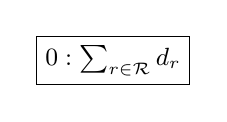
\begin{tikzpicture}
\small
\matrix[nodes={minimum size=6mm}] {
  \node[draw] {$0:\sum_{r\in\mathcal{R}}d_r$};\\
};
\end{tikzpicture}\\
\textbf{Side Effects:} none.\\
\textbf{Throws:} {\tt{}SQLException} if database failure is encountered.\\
\bottomrule
\end{tabular}
\nwenddocs{}\nwbegincode{172}\sublabel{NW18ZcDF-3ddWJ0-1}\nwmargintag{{\nwtagstyle{}\subpageref{NW18ZcDF-3ddWJ0-1}}}\moddef{Read: DBQueryMetricRequestDistanceBaseTotal(0)~{\nwtagstyle{}\subpageref{NW18ZcDF-3ddWJ0-1}}}\endmoddef\nwused{\\{NW3x1zuR-Oyob-1}}
int[] DBQueryMetricRequestDistanceBaseTotal() throws SQLException \{
  try (\LA{}Open \code{}conn\edoc{}~{\nwtagstyle{}\subpageref{NWgUSr6-JT1v9-1}}\RA{}) \{
    return PSQuery(conn, "S111", 1);
  \} catch (SQLException e) \{
    throw e;
  \}
\}
\nwindexdefn{DBQueryMetricRequestDistanceBaseTotal}{DBQueryMetricRequestDistanceBaseTotal}{NW18ZcDF-3ddWJ0-1}\eatline
\nwidentdefs{\\{{DBQueryMetricRequestDistanceBaseTotal}{DBQueryMetricRequestDistanceBaseTotal}}}\nwidentuses{\\{{PSQuery}{PSQuery}}\\{{S111}{S111}}}\nwindexuse{PSQuery}{PSQuery}{NW18ZcDF-3ddWJ0-1}\nwindexuse{S111}{S111}{NW18ZcDF-3ddWJ0-1}\nwendcode{}\nwbegindocs{173}\begin{tabular}{p{\textwidth}}
\toprule
\rowcolor{TableTitle}
Method \textcolor{blue}{{\tt{}\protect\nwindexuse{queryMetricRequestDistanceBaseTotal}{queryMetricRequestDistanceBaseTotal}{NW18ZcDF-v7TDa-1}queryMetricRequestDistanceBaseTotal}}(0) wraps {\tt{}\protect\nwindexuse{DBQueryMetricRequestDistanceBaseTotal}{DBQueryMetricRequestDistanceBaseTotal}{NW18ZcDF-3ddWJ0-1}DBQueryMetricRequestDistanceBaseTotal}(0).\\
\bottomrule
\end{tabular}
\nwenddocs{}\nwbegincode{174}\sublabel{NW18ZcDF-v7TDa-1}\nwmargintag{{\nwtagstyle{}\subpageref{NW18ZcDF-v7TDa-1}}}\moddef{Read: queryMetricRequestDistanceBaseTotal(0)~{\nwtagstyle{}\subpageref{NW18ZcDF-v7TDa-1}}}\endmoddef\nwused{\\{NW3x1zuR-2u8vSA-1}}
int[] queryMetricRequestDistanceBaseTotal() throws SQLException \{
  return storage.DBQueryMetricRequestDistanceBaseTotal();
\}
\nwindexdefn{queryMetricRequestDistanceBaseTotal}{queryMetricRequestDistanceBaseTotal}{NW18ZcDF-v7TDa-1}\eatline
\nwidentdefs{\\{{queryMetricRequestDistanceBaseTotal}{queryMetricRequestDistanceBaseTotal}}}\nwidentuses{\\{{DBQueryMetricRequestDistanceBaseTotal}{DBQueryMetricRequestDistanceBaseTotal}}}\nwindexuse{DBQueryMetricRequestDistanceBaseTotal}{DBQueryMetricRequestDistanceBaseTotal}{NW18ZcDF-v7TDa-1}\nwendcode{}\nwbegindocs{175}\nwdocspar
\subsection{\texttt{DBQueryMetricRequestDistanceBaseUnassignedTotal}(0)}
\begin{tabular}{p{\textwidth}}
\toprule
\rowcolor{TableTitle}
Method \textcolor{blue}{{\tt{}\protect\nwindexuse{DBQueryMetricRequestDistanceBaseUnassignedTotal}{DBQueryMetricRequestDistanceBaseUnassignedTotal}{NW18ZcDF-421s5A-1}DBQueryMetricRequestDistanceBaseUnassignedTotal}}(0) returns the
base distance of all the unassigned requests.
A {\tt{}SQLException} is thrown in case of database failure.\\
\midrule
\textbf{Parameters:} none.\\
\textbf{Returns:} results of the query flattened into an integer array,
or {\tt{}null} if no results.

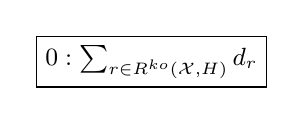
\begin{tikzpicture}
\small
\matrix[nodes={minimum size=6mm}] {
  \node[draw] {$0:\sum_{r\in R^{ko}(\mathcal{X},H)}d_r$};\\
};
\end{tikzpicture}

where $H$ is the time horizon.\\
\textbf{Side Effects:} none.\\
\textbf{Throws:} {\tt{}SQLException} if database failure is encountered.\\
\bottomrule
\end{tabular}
\nwenddocs{}\nwbegincode{176}\sublabel{NW18ZcDF-421s5A-1}\nwmargintag{{\nwtagstyle{}\subpageref{NW18ZcDF-421s5A-1}}}\moddef{Read: DBQueryMetricRequestDistanceBaseUnassignedTotal(0)~{\nwtagstyle{}\subpageref{NW18ZcDF-421s5A-1}}}\endmoddef\nwused{\\{NW3x1zuR-Oyob-1}}
int[] DBQueryMetricRequestDistanceBaseUnassignedTotal() throws SQLException \{
  try (\LA{}Open \code{}conn\edoc{}~{\nwtagstyle{}\subpageref{NWgUSr6-JT1v9-1}}\RA{}) \{
    return PSQuery(conn, "S138", 1);
  \} catch (SQLException e) \{
    throw e;
  \}
\}
\nwindexdefn{DBQueryMetricRequestDistanceBaseUnassignedTotal}{DBQueryMetricRequestDistanceBaseUnassignedTotal}{NW18ZcDF-421s5A-1}\eatline
\nwidentdefs{\\{{DBQueryMetricRequestDistanceBaseUnassignedTotal}{DBQueryMetricRequestDistanceBaseUnassignedTotal}}}\nwidentuses{\\{{PSQuery}{PSQuery}}\\{{S138}{S138}}}\nwindexuse{PSQuery}{PSQuery}{NW18ZcDF-421s5A-1}\nwindexuse{S138}{S138}{NW18ZcDF-421s5A-1}\nwendcode{}\nwbegindocs{177}\begin{tabular}{p{\textwidth}}
\toprule
\rowcolor{TableTitle}
Method \textcolor{blue}{{\tt{}\protect\nwindexuse{queryMetricRequestDistanceBaseUnassignedTotal}{queryMetricRequestDistanceBaseUnassignedTotal}{NW18ZcDF-4H3t3H-1}queryMetricRequestDistanceBaseUnassignedTotal}}(0) wraps {\tt{}\protect\nwindexuse{DBQueryMetricRequestDistanceBaseUnassignedTotal}{DBQueryMetricRequestDistanceBaseUnassignedTotal}{NW18ZcDF-421s5A-1}DBQueryMetricRequestDistanceBaseUnassignedTotal}(0).\\
\bottomrule
\end{tabular}
\nwenddocs{}\nwbegincode{178}\sublabel{NW18ZcDF-4H3t3H-1}\nwmargintag{{\nwtagstyle{}\subpageref{NW18ZcDF-4H3t3H-1}}}\moddef{Read: queryMetricRequestDistanceBaseUnassignedTotal(0)~{\nwtagstyle{}\subpageref{NW18ZcDF-4H3t3H-1}}}\endmoddef\nwused{\\{NW3x1zuR-2u8vSA-1}}
int[] queryMetricRequestDistanceBaseUnassignedTotal() throws SQLException \{
  return storage.DBQueryMetricRequestDistanceBaseUnassignedTotal();
\}
\nwindexdefn{queryMetricRequestDistanceBaseUnassignedTotal}{queryMetricRequestDistanceBaseUnassignedTotal}{NW18ZcDF-4H3t3H-1}\eatline
\nwidentdefs{\\{{queryMetricRequestDistanceBaseUnassignedTotal}{queryMetricRequestDistanceBaseUnassignedTotal}}}\nwidentuses{\\{{DBQueryMetricRequestDistanceBaseUnassignedTotal}{DBQueryMetricRequestDistanceBaseUnassignedTotal}}}\nwindexuse{DBQueryMetricRequestDistanceBaseUnassignedTotal}{DBQueryMetricRequestDistanceBaseUnassignedTotal}{NW18ZcDF-4H3t3H-1}\nwendcode{}\nwbegindocs{179}\nwdocspar
\subsection{\texttt{DBQueryMetricRequestDistanceDetourTotal}(0)}
\begin{tabular}{p{\textwidth}}
\toprule
\rowcolor{TableTitle}
Method \textcolor{blue}{{\tt{}\protect\nwindexuse{DBQueryMetricRequestDistanceDetourTotal}{DBQueryMetricRequestDistanceDetourTotal}{NW18ZcDF-3066Ie-1}DBQueryMetricRequestDistanceDetourTotal}}(0) returns the
total detour distance of all requests.
A {\tt{}SQLException} is thrown in case of database failure.\\
\midrule
\textbf{Parameters:} none.\\
\textbf{Returns:} results of the query flattened into an integer array,
or {\tt{}null} if no results.

\begin{tikzpicture}
\small
\matrix[nodes={minimum size=6mm}] {
  \node[draw] {$0:\sum_{r\in\mathcal{R}}D^\textrm{detour}(\mathcal{X},r)$};\\
};
\end{tikzpicture}\\
\textbf{Side Effects:} none.\\
\textbf{Throws:} {\tt{}SQLException} if database failure is encountered.\\
\bottomrule
\end{tabular}
\nwenddocs{}\nwbegincode{180}\sublabel{NW18ZcDF-3066Ie-1}\nwmargintag{{\nwtagstyle{}\subpageref{NW18ZcDF-3066Ie-1}}}\moddef{Read: DBQueryMetricRequestDistanceDetourTotal(0)~{\nwtagstyle{}\subpageref{NW18ZcDF-3066Ie-1}}}\endmoddef\nwused{\\{NW3x1zuR-Oyob-1}}
int[] DBQueryMetricRequestDistanceDetourTotal() throws SQLException \{
  try (\LA{}Open \code{}conn\edoc{}~{\nwtagstyle{}\subpageref{NWgUSr6-JT1v9-1}}\RA{}) \{
    return PSQuery(conn, "S113", 1);
  \} catch (SQLException e) \{
    throw e;
  \}
\}
\nwindexdefn{DBQueryMetricRequestDistanceDetourTotal}{DBQueryMetricRequestDistanceDetourTotal}{NW18ZcDF-3066Ie-1}\eatline
\nwidentdefs{\\{{DBQueryMetricRequestDistanceDetourTotal}{DBQueryMetricRequestDistanceDetourTotal}}}\nwidentuses{\\{{PSQuery}{PSQuery}}\\{{S113}{S113}}}\nwindexuse{PSQuery}{PSQuery}{NW18ZcDF-3066Ie-1}\nwindexuse{S113}{S113}{NW18ZcDF-3066Ie-1}\nwendcode{}\nwbegindocs{181}\begin{tabular}{p{\textwidth}}
\toprule
\rowcolor{TableTitle}
Method \textcolor{blue}{{\tt{}\protect\nwindexuse{queryMetricRequestDistanceDetourTotal}{queryMetricRequestDistanceDetourTotal}{NW18ZcDF-1GQ2zQ-1}queryMetricRequestDistanceDetourTotal}}(0) wraps {\tt{}\protect\nwindexuse{DBQueryMetricRequestDistanceDetourTotal}{DBQueryMetricRequestDistanceDetourTotal}{NW18ZcDF-3066Ie-1}DBQueryMetricRequestDistanceDetourTotal}(0).\\
\bottomrule
\end{tabular}
\nwenddocs{}\nwbegincode{182}\sublabel{NW18ZcDF-1GQ2zQ-1}\nwmargintag{{\nwtagstyle{}\subpageref{NW18ZcDF-1GQ2zQ-1}}}\moddef{Read: queryMetricRequestDistanceDetourTotal(0)~{\nwtagstyle{}\subpageref{NW18ZcDF-1GQ2zQ-1}}}\endmoddef\nwused{\\{NW3x1zuR-2u8vSA-1}}
int[] queryMetricRequestDistanceDetourTotal() throws SQLException \{
  return storage.DBQueryMetricRequestDistanceDetourTotal();
\}
\nwindexdefn{queryMetricRequestDistanceDetourTotal}{queryMetricRequestDistanceDetourTotal}{NW18ZcDF-1GQ2zQ-1}\eatline
\nwidentdefs{\\{{queryMetricRequestDistanceDetourTotal}{queryMetricRequestDistanceDetourTotal}}}\nwidentuses{\\{{DBQueryMetricRequestDistanceDetourTotal}{DBQueryMetricRequestDistanceDetourTotal}}}\nwindexuse{DBQueryMetricRequestDistanceDetourTotal}{DBQueryMetricRequestDistanceDetourTotal}{NW18ZcDF-1GQ2zQ-1}\nwendcode{}\nwbegindocs{183}\nwdocspar
\subsection{\texttt{DBQueryMetricRequestDistanceTransitTotal}(0)}
\begin{tabular}{p{\textwidth}}
\toprule
\rowcolor{TableTitle}
Method \textcolor{blue}{{\tt{}\protect\nwindexuse{DBQueryMetricRequestDistanceTransitTotal}{DBQueryMetricRequestDistanceTransitTotal}{NW18ZcDF-Z4xun-1}DBQueryMetricRequestDistanceTransitTotal}}(0) returns the
total transit distance of all requests.
A {\tt{}SQLException} is thrown in case of database failure.\\
\midrule
\textbf{Parameters:} none.\\
\textbf{Returns:} results of the query flattened into an integer array,
or {\tt{}null} if no results.

\begin{tikzpicture}
\small
\matrix[nodes={minimum size=6mm}] {
  \node[draw] {$0:\sum_{r\in\mathcal{R}}D^\textrm{transit}(\mathcal{X},r)$};\\
};
\end{tikzpicture}\\
\textbf{Side Effects:} none.\\
\textbf{Throws:} {\tt{}SQLException} if database failure is encountered.\\
\bottomrule
\end{tabular}
\nwenddocs{}\nwbegincode{184}\sublabel{NW18ZcDF-Z4xun-1}\nwmargintag{{\nwtagstyle{}\subpageref{NW18ZcDF-Z4xun-1}}}\moddef{Read: DBQueryMetricRequestDistanceTransitTotal(0)~{\nwtagstyle{}\subpageref{NW18ZcDF-Z4xun-1}}}\endmoddef\nwused{\\{NW3x1zuR-Oyob-1}}
int[] DBQueryMetricRequestDistanceTransitTotal() throws SQLException \{
  try (\LA{}Open \code{}conn\edoc{}~{\nwtagstyle{}\subpageref{NWgUSr6-JT1v9-1}}\RA{}) \{
    return PSQuery(conn, "S115", 1);
  \} catch (SQLException e) \{
    throw e;
  \}
\}
\nwindexdefn{DBQueryMetricRequestDistanceTransitTotal}{DBQueryMetricRequestDistanceTransitTotal}{NW18ZcDF-Z4xun-1}\eatline
\nwidentdefs{\\{{DBQueryMetricRequestDistanceTransitTotal}{DBQueryMetricRequestDistanceTransitTotal}}}\nwidentuses{\\{{PSQuery}{PSQuery}}\\{{S115}{S115}}}\nwindexuse{PSQuery}{PSQuery}{NW18ZcDF-Z4xun-1}\nwindexuse{S115}{S115}{NW18ZcDF-Z4xun-1}\nwendcode{}\nwbegindocs{185}\begin{tabular}{p{\textwidth}}
\toprule
\rowcolor{TableTitle}
Method \textcolor{blue}{{\tt{}\protect\nwindexuse{queryMetricRequestDistanceTransitTotal}{queryMetricRequestDistanceTransitTotal}{NW18ZcDF-l8wOt-1}queryMetricRequestDistanceTransitTotal}}(0) wraps {\tt{}\protect\nwindexuse{DBQueryMetricRequestDistanceTransitTotal}{DBQueryMetricRequestDistanceTransitTotal}{NW18ZcDF-Z4xun-1}DBQueryMetricRequestDistanceTransitTotal}(0).\\
\bottomrule
\end{tabular}
\nwenddocs{}\nwbegincode{186}\sublabel{NW18ZcDF-l8wOt-1}\nwmargintag{{\nwtagstyle{}\subpageref{NW18ZcDF-l8wOt-1}}}\moddef{Read: queryMetricRequestDistanceTransitTotal(0)~{\nwtagstyle{}\subpageref{NW18ZcDF-l8wOt-1}}}\endmoddef\nwused{\\{NW3x1zuR-2u8vSA-1}}
int[] queryMetricRequestDistanceTransitTotal() throws SQLException \{
  return storage.DBQueryMetricRequestDistanceTransitTotal();
\}
\nwindexdefn{queryMetricRequestDistanceTransitTotal}{queryMetricRequestDistanceTransitTotal}{NW18ZcDF-l8wOt-1}\eatline
\nwidentdefs{\\{{queryMetricRequestDistanceTransitTotal}{queryMetricRequestDistanceTransitTotal}}}\nwidentuses{\\{{DBQueryMetricRequestDistanceTransitTotal}{DBQueryMetricRequestDistanceTransitTotal}}}\nwindexuse{DBQueryMetricRequestDistanceTransitTotal}{DBQueryMetricRequestDistanceTransitTotal}{NW18ZcDF-l8wOt-1}\nwendcode{}\nwbegindocs{187}\nwdocspar
\subsection{\texttt{DBQueryMetricRequestDurationPickupTotal}(0)}
\begin{tabular}{p{\textwidth}}
\toprule
\rowcolor{TableTitle}
Method \textcolor{blue}{{\tt{}\protect\nwindexuse{DBQueryMetricRequestDurationPickupTotal}{DBQueryMetricRequestDurationPickupTotal}{NW18ZcDF-28z28Y-1}DBQueryMetricRequestDurationPickupTotal}}(0) returns the
total pickup delay of all requests.
A {\tt{}SQLException} is thrown in case of database failure.\\
\midrule
\textbf{Parameters:} none.\\
\textbf{Returns:} results of the query flattened into an integer array,
or {\tt{}null} if no results.

\begin{tikzpicture}
\small
\matrix[nodes={minimum size=6mm}] {
  \node[draw] {$0:\sum_{r\in\mathcal{R}}\delta^\textrm{pickup}(\mathcal{X},r)$};\\
};
\end{tikzpicture}\\
\textbf{Side Effects:} none.\\
\textbf{Throws:} {\tt{}SQLException} if database failure is encountered.\\
\bottomrule
\end{tabular}
\nwenddocs{}\nwbegincode{188}\sublabel{NW18ZcDF-28z28Y-1}\nwmargintag{{\nwtagstyle{}\subpageref{NW18ZcDF-28z28Y-1}}}\moddef{Read: DBQueryMetricRequestDurationPickupTotal(0)~{\nwtagstyle{}\subpageref{NW18ZcDF-28z28Y-1}}}\endmoddef\nwused{\\{NW3x1zuR-Oyob-1}}
int[] DBQueryMetricRequestDurationPickupTotal() throws SQLException \{
  try (\LA{}Open \code{}conn\edoc{}~{\nwtagstyle{}\subpageref{NWgUSr6-JT1v9-1}}\RA{}) \{
    return PSQuery(conn, "S119", 1);
  \} catch (SQLException e) \{
    throw e;
  \}
\}
\nwindexdefn{DBQueryMetricRequestDurationPickupTotal}{DBQueryMetricRequestDurationPickupTotal}{NW18ZcDF-28z28Y-1}\eatline
\nwidentdefs{\\{{DBQueryMetricRequestDurationPickupTotal}{DBQueryMetricRequestDurationPickupTotal}}}\nwidentuses{\\{{PSQuery}{PSQuery}}\\{{S119}{S119}}}\nwindexuse{PSQuery}{PSQuery}{NW18ZcDF-28z28Y-1}\nwindexuse{S119}{S119}{NW18ZcDF-28z28Y-1}\nwendcode{}\nwbegindocs{189}\begin{tabular}{p{\textwidth}}
\toprule
\rowcolor{TableTitle}
Method \textcolor{blue}{{\tt{}\protect\nwindexuse{queryMetricRequestDurationPickupTotal}{queryMetricRequestDurationPickupTotal}{NW18ZcDF-2hwTtW-1}queryMetricRequestDurationPickupTotal}}(0) wraps {\tt{}\protect\nwindexuse{DBQueryMetricRequestDurationPickupTotal}{DBQueryMetricRequestDurationPickupTotal}{NW18ZcDF-28z28Y-1}DBQueryMetricRequestDurationPickupTotal}(0).\\
\bottomrule
\end{tabular}
\nwenddocs{}\nwbegincode{190}\sublabel{NW18ZcDF-2hwTtW-1}\nwmargintag{{\nwtagstyle{}\subpageref{NW18ZcDF-2hwTtW-1}}}\moddef{Read: queryMetricRequestDurationPickupTotal(0)~{\nwtagstyle{}\subpageref{NW18ZcDF-2hwTtW-1}}}\endmoddef\nwused{\\{NW3x1zuR-2u8vSA-1}}
int[] queryMetricRequestDurationPickupTotal() throws SQLException \{
  return storage.DBQueryMetricRequestDurationPickupTotal();
\}
\nwindexdefn{queryMetricRequestDurationPickupTotal}{queryMetricRequestDurationPickupTotal}{NW18ZcDF-2hwTtW-1}\eatline
\nwidentdefs{\\{{queryMetricRequestDurationPickupTotal}{queryMetricRequestDurationPickupTotal}}}\nwidentuses{\\{{DBQueryMetricRequestDurationPickupTotal}{DBQueryMetricRequestDurationPickupTotal}}}\nwindexuse{DBQueryMetricRequestDurationPickupTotal}{DBQueryMetricRequestDurationPickupTotal}{NW18ZcDF-2hwTtW-1}\nwendcode{}\nwbegindocs{191}\nwdocspar
\subsection{\texttt{DBQueryMetricRequestDurationTransitTotal}(0)}
\begin{tabular}{p{\textwidth}}
\toprule
\rowcolor{TableTitle}
Method \textcolor{blue}{{\tt{}\protect\nwindexuse{DBQueryMetricRequestDurationTransitTotal}{DBQueryMetricRequestDurationTransitTotal}{NW18ZcDF-2RC1QH-1}DBQueryMetricRequestDurationTransitTotal}}(0) returns the
total transit duration of all requests.
A {\tt{}SQLException} is thrown in case of database failure.\\
\midrule
\textbf{Parameters:} none.\\
\textbf{Returns:} results of the query flattened into an integer array,
or {\tt{}null} if no results.

\begin{tikzpicture}
\small
\matrix[nodes={minimum size=6mm}] {
  \node[draw] {$0:\sum_{r\in\mathcal{R}}\delta^\textrm{transit}(\mathcal{X},r)$};\\
};
\end{tikzpicture}\\
\textbf{Side Effects:} none.\\
\textbf{Throws:} {\tt{}SQLException} if database failure is encountered.\\
\bottomrule
\end{tabular}
\nwenddocs{}\nwbegincode{192}\sublabel{NW18ZcDF-2RC1QH-1}\nwmargintag{{\nwtagstyle{}\subpageref{NW18ZcDF-2RC1QH-1}}}\moddef{Read: DBQueryMetricRequestDurationTransitTotal(0)~{\nwtagstyle{}\subpageref{NW18ZcDF-2RC1QH-1}}}\endmoddef\nwused{\\{NW3x1zuR-Oyob-1}}
int[] DBQueryMetricRequestDurationTransitTotal() throws SQLException \{
  try (\LA{}Open \code{}conn\edoc{}~{\nwtagstyle{}\subpageref{NWgUSr6-JT1v9-1}}\RA{}) \{
    return PSQuery(conn, "S121", 1);
  \} catch (SQLException e) \{
    throw e;
  \}
\}
\nwindexdefn{DBQueryMetricRequestDurationTransitTotal}{DBQueryMetricRequestDurationTransitTotal}{NW18ZcDF-2RC1QH-1}\eatline
\nwidentdefs{\\{{DBQueryMetricRequestDurationTransitTotal}{DBQueryMetricRequestDurationTransitTotal}}}\nwidentuses{\\{{PSQuery}{PSQuery}}\\{{S121}{S121}}}\nwindexuse{PSQuery}{PSQuery}{NW18ZcDF-2RC1QH-1}\nwindexuse{S121}{S121}{NW18ZcDF-2RC1QH-1}\nwendcode{}\nwbegindocs{193}\begin{tabular}{p{\textwidth}}
\toprule
\rowcolor{TableTitle}
Method \textcolor{blue}{{\tt{}\protect\nwindexuse{queryMetricRequestDurationTransitTotal}{queryMetricRequestDurationTransitTotal}{NW18ZcDF-3GQbSd-1}queryMetricRequestDurationTransitTotal}}(0) wraps {\tt{}\protect\nwindexuse{DBQueryMetricRequestDurationTransitTotal}{DBQueryMetricRequestDurationTransitTotal}{NW18ZcDF-2RC1QH-1}DBQueryMetricRequestDurationTransitTotal}(0).\\
\bottomrule
\end{tabular}
\nwenddocs{}\nwbegincode{194}\sublabel{NW18ZcDF-3GQbSd-1}\nwmargintag{{\nwtagstyle{}\subpageref{NW18ZcDF-3GQbSd-1}}}\moddef{Read: queryMetricRequestDurationTransitTotal(0)~{\nwtagstyle{}\subpageref{NW18ZcDF-3GQbSd-1}}}\endmoddef\nwused{\\{NW3x1zuR-2u8vSA-1}}
int[] queryMetricRequestDurationTransitTotal() throws SQLException \{
  return storage.DBQueryMetricRequestDurationTransitTotal();
\}
\nwindexdefn{queryMetricRequestDurationTransitTotal}{queryMetricRequestDurationTransitTotal}{NW18ZcDF-3GQbSd-1}\eatline
\nwidentdefs{\\{{queryMetricRequestDurationTransitTotal}{queryMetricRequestDurationTransitTotal}}}\nwidentuses{\\{{DBQueryMetricRequestDurationTransitTotal}{DBQueryMetricRequestDurationTransitTotal}}}\nwindexuse{DBQueryMetricRequestDurationTransitTotal}{DBQueryMetricRequestDurationTransitTotal}{NW18ZcDF-3GQbSd-1}\nwendcode{}\nwbegindocs{195}\nwdocspar
\subsection{\texttt{DBQueryMetricRequestDurationTravelTotal}(0)}
\begin{tabular}{p{\textwidth}}
\toprule
\rowcolor{TableTitle}
Method \textcolor{blue}{{\tt{}\protect\nwindexuse{DBQueryMetricRequestDurationTravelTotal}{DBQueryMetricRequestDurationTravelTotal}{NW18ZcDF-3y4D9i-1}DBQueryMetricRequestDurationTravelTotal}}(0) returns the
total travel duration of all requests.
A {\tt{}SQLException} is thrown in case of database failure.\\
\midrule
\textbf{Parameters:} none.\\
\textbf{Returns:} results of the query flattened into an integer array,
or {\tt{}null} if no results.

\begin{tikzpicture}
\small
\matrix[nodes={minimum size=6mm}] {
  \node[draw] {$0:\sum_{r\in\mathcal{R}}\delta^\textrm{travel}(\mathcal{X},r)$};\\
};
\end{tikzpicture}\\
\textbf{Side Effects:} none.\\
\textbf{Throws:} {\tt{}SQLException} if database failure is encountered.\\
\bottomrule
\end{tabular}
\nwenddocs{}\nwbegincode{196}\sublabel{NW18ZcDF-3y4D9i-1}\nwmargintag{{\nwtagstyle{}\subpageref{NW18ZcDF-3y4D9i-1}}}\moddef{Read: DBQueryMetricRequestDurationTravelTotal(0)~{\nwtagstyle{}\subpageref{NW18ZcDF-3y4D9i-1}}}\endmoddef\nwused{\\{NW3x1zuR-Oyob-1}}
int[] DBQueryMetricRequestDurationTravelTotal() throws SQLException \{
  try (\LA{}Open \code{}conn\edoc{}~{\nwtagstyle{}\subpageref{NWgUSr6-JT1v9-1}}\RA{}) \{
    return PSQuery(conn, "S123", 1);
  \} catch (SQLException e) \{
    throw e;
  \}
\}
\nwindexdefn{DBQueryMetricRequestDurationTravelTotal}{DBQueryMetricRequestDurationTravelTotal}{NW18ZcDF-3y4D9i-1}\eatline
\nwidentdefs{\\{{DBQueryMetricRequestDurationTravelTotal}{DBQueryMetricRequestDurationTravelTotal}}}\nwidentuses{\\{{PSQuery}{PSQuery}}\\{{S123}{S123}}}\nwindexuse{PSQuery}{PSQuery}{NW18ZcDF-3y4D9i-1}\nwindexuse{S123}{S123}{NW18ZcDF-3y4D9i-1}\nwendcode{}\nwbegindocs{197}\begin{tabular}{p{\textwidth}}
\toprule
\rowcolor{TableTitle}
Method \textcolor{blue}{{\tt{}\protect\nwindexuse{queryMetricRequestDurationTravelTotal}{queryMetricRequestDurationTravelTotal}{NW18ZcDF-18k7oI-1}queryMetricRequestDurationTravelTotal}}(0) wraps {\tt{}\protect\nwindexuse{DBQueryMetricRequestDurationTravelTotal}{DBQueryMetricRequestDurationTravelTotal}{NW18ZcDF-3y4D9i-1}DBQueryMetricRequestDurationTravelTotal}(0).\\
\bottomrule
\end{tabular}
\nwenddocs{}\nwbegincode{198}\sublabel{NW18ZcDF-18k7oI-1}\nwmargintag{{\nwtagstyle{}\subpageref{NW18ZcDF-18k7oI-1}}}\moddef{Read: queryMetricRequestDurationTravelTotal(0)~{\nwtagstyle{}\subpageref{NW18ZcDF-18k7oI-1}}}\endmoddef\nwused{\\{NW3x1zuR-2u8vSA-1}}
int[] queryMetricRequestDurationTravelTotal() throws SQLException \{
  return storage.DBQueryMetricRequestDurationTravelTotal();
\}
\nwindexdefn{queryMetricRequestDurationTravelTotal}{queryMetricRequestDurationTravelTotal}{NW18ZcDF-18k7oI-1}\eatline
\nwidentdefs{\\{{queryMetricRequestDurationTravelTotal}{queryMetricRequestDurationTravelTotal}}}\nwidentuses{\\{{DBQueryMetricRequestDurationTravelTotal}{DBQueryMetricRequestDurationTravelTotal}}}\nwindexuse{DBQueryMetricRequestDurationTravelTotal}{DBQueryMetricRequestDurationTravelTotal}{NW18ZcDF-18k7oI-1}\nwendcode{}\nwbegindocs{199}\nwdocspar
\subsection{\texttt{DBQueryMetricRequestTWViolationsTotal}(0)}
\nwenddocs{}\nwbegincode{200}\sublabel{NW18ZcDF-4Q7d2w-1}\nwmargintag{{\nwtagstyle{}\subpageref{NW18ZcDF-4Q7d2w-1}}}\moddef{Read: DBQueryMetricRequestTWViolationsTotal(0)~{\nwtagstyle{}\subpageref{NW18ZcDF-4Q7d2w-1}}}\endmoddef\nwused{\\{NW3x1zuR-Oyob-1}}
int[] DBQueryMetricRequestTWViolationsTotal() throws SQLException \{
  try (\LA{}Open \code{}conn\edoc{}~{\nwtagstyle{}\subpageref{NWgUSr6-JT1v9-1}}\RA{}) \{
    return PSQuery(conn, "S151", 2);
  \} catch (SQLException e) \{
    throw e;
  \}
\}
\nwindexdefn{DBQueryMetricRequestTWViolationsTotal}{DBQueryMetricRequestTWViolationsTotal}{NW18ZcDF-4Q7d2w-1}\eatline
\nwidentdefs{\\{{DBQueryMetricRequestTWViolationsTotal}{DBQueryMetricRequestTWViolationsTotal}}}\nwidentuses{\\{{PSQuery}{PSQuery}}\\{{S151}{S151}}}\nwindexuse{PSQuery}{PSQuery}{NW18ZcDF-4Q7d2w-1}\nwindexuse{S151}{S151}{NW18ZcDF-4Q7d2w-1}\nwendcode{}\nwbegincode{201}\sublabel{NW18ZcDF-6MUNa-1}\nwmargintag{{\nwtagstyle{}\subpageref{NW18ZcDF-6MUNa-1}}}\moddef{Read: queryMetricRequestTWViolationsTotal(0)~{\nwtagstyle{}\subpageref{NW18ZcDF-6MUNa-1}}}\endmoddef\nwused{\\{NW3x1zuR-2u8vSA-1}}
int[] queryMetricRequestTWViolationsTotal() throws SQLException \{
  return storage.DBQueryMetricRequestTWViolationsTotal();
\}
\nwindexdefn{queryMetricRequestTWViolationsTotal}{queryMetricRequestTWViolationsTotal}{NW18ZcDF-6MUNa-1}\eatline
\nwidentdefs{\\{{queryMetricRequestTWViolationsTotal}{queryMetricRequestTWViolationsTotal}}}\nwidentuses{\\{{DBQueryMetricRequestTWViolationsTotal}{DBQueryMetricRequestTWViolationsTotal}}}\nwindexuse{DBQueryMetricRequestTWViolationsTotal}{DBQueryMetricRequestTWViolationsTotal}{NW18ZcDF-6MUNa-1}\nwendcode{}\nwfilename{src/tex/3-Writing.nw}\nwbegindocs{0}\chapter{Write Operations}
\label{write}

\section{Chunks}

\subsection{Apply traffic to route, sched}
\nwenddocs{}\nwbegincode{1}\sublabel{NW32V2DP-UeHS0-1}\nwmargintag{{\nwtagstyle{}\subpageref{NW32V2DP-UeHS0-1}}}\moddef{Apply traffic to route, sched~{\nwtagstyle{}\subpageref{NW32V2DP-UeHS0-1}}}\endmoddef\nwused{\\{NW32V2DP-3PimUR-1}\\{NW32V2DP-42pL1g-1}\\{NW32V2DP-3O61Nf-1}}
int[] mutroute = route.clone();
int[] mutsched = sched.clone();
if (this.traffic != null) \{
  for (int k = 0; k < (mutroute.length - 3); k += 4) \{
    final int t1 = mutroute[k];
    final int v1 = mutroute[(k + 1)];
    final int t2 = mutroute[(k + 2)];
    final int v2 = mutroute[(k + 3)];
    int[] ddnu = this.storage.DBQueryEdge(v1, v2);
    final int dd = ddnu[0];
    final int nu_old = ddnu[1];
    final int nu_new = Math.max(1, (int) Math.round(this.traffic.apply(v1, v2, t1)*nu_old));
    final int diff = ((dd/(t2 - t1)) > nu_new
        ? ((int) Math.ceil((dd/(float) nu_new + t1))) - t2
        : 0);
    if (diff != 0) \{
      for (int p = 0; p < (mutsched.length - 2); p += 3) \{
        if (mutsched[p] >= mutroute[(k + 2)]) \{
          mutsched[p] += diff;
        \}
      \}
      for (int q = (k + 2); q < (mutroute.length - 1); q += 2) \{
        mutroute[q] += diff;
      \}
    \}
  \}
\}
\nwidentuses{\\{{apply}{apply}}\\{{DBQueryEdge}{DBQueryEdge}}}\nwindexuse{apply}{apply}{NW32V2DP-UeHS0-1}\nwindexuse{DBQueryEdge}{DBQueryEdge}{NW32V2DP-UeHS0-1}\nwendcode{}\nwbegindocs{2}\nwdocspar

\subsection{Check time window violation}
\nwenddocs{}\nwbegincode{3}\sublabel{NW32V2DP-3kBClV-1}\nwmargintag{{\nwtagstyle{}\subpageref{NW32V2DP-3kBClV-1}}}\moddef{Check time window violation~{\nwtagstyle{}\subpageref{NW32V2DP-3kBClV-1}}}\endmoddef\nwused{\\{NW32V2DP-3PimUR-1}\\{NW32V2DP-42pL1g-1}\\{NW32V2DP-3O61Nf-1}}
for (int k = 0; k < (sched.length - 2); k += 3) \{
  final int tl = this.storage.DBQueryUser(sched[(k + 2)])[3];
  if (sched[k] > tl) \{
    throw new TimeWindowException("Waypoint time (t="+sched[k]+") "
        +"after late window (t="+tl+", uid="+sched[(k + 2)]+")");
  \}
\}
\nwidentuses{\\{{DBQueryUser}{DBQueryUser}}}\nwindexuse{DBQueryUser}{DBQueryUser}{NW32V2DP-3kBClV-1}\nwendcode{}\nwbegindocs{4}\nwdocspar

\subsection{Delete from W remaining route}
\nwenddocs{}\nwbegincode{5}\sublabel{NW32V2DP-3yaRFT-1}\nwmargintag{{\nwtagstyle{}\subpageref{NW32V2DP-3yaRFT-1}}}\moddef{Delete from W remaining route~{\nwtagstyle{}\subpageref{NW32V2DP-3yaRFT-1}}}\endmoddef\nwused{\\{NW32V2DP-3RBwFo-1}}
PreparedStatement pS76 = this.PSCreate(conn, "S76");
this.PSAdd(pS76, sid, route[0]);
this.PSSubmit(pS76);
\nwidentuses{\\{{PSAdd}{PSAdd}}\\{{PSCreate}{PSCreate}}\\{{PSSubmit}{PSSubmit}}\\{{S76}{S76}}}\nwindexuse{PSAdd}{PSAdd}{NW32V2DP-3yaRFT-1}\nwindexuse{PSCreate}{PSCreate}{NW32V2DP-3yaRFT-1}\nwindexuse{PSSubmit}{PSSubmit}{NW32V2DP-3yaRFT-1}\nwindexuse{S76}{S76}{NW32V2DP-3yaRFT-1}\nwendcode{}\nwbegindocs{6}\nwdocspar

\subsection{Delete from PD, CPD jobs}
\nwenddocs{}\nwbegincode{7}\sublabel{NW32V2DP-KKb67-1}\nwmargintag{{\nwtagstyle{}\subpageref{NW32V2DP-KKb67-1}}}\moddef{Delete from PD, CPD jobs~{\nwtagstyle{}\subpageref{NW32V2DP-KKb67-1}}}\endmoddef\nwused{\\{NW32V2DP-PxyQL-1}}
PreparedStatement pS42 = this.PSCreate(conn, "S42");
PreparedStatement pS43 = this.PSCreate(conn, "S43");
for (final int r : rid) \{
  this.PSAdd(pS42, r);
  this.PSAdd(pS43, r);
\}
this.PSSubmit(pS42, pS43);
\nwidentuses{\\{{PSAdd}{PSAdd}}\\{{PSCreate}{PSCreate}}\\{{PSSubmit}{PSSubmit}}\\{{S42}{S42}}\\{{S43}{S43}}}\nwindexuse{PSAdd}{PSAdd}{NW32V2DP-KKb67-1}\nwindexuse{PSCreate}{PSCreate}{NW32V2DP-KKb67-1}\nwindexuse{PSSubmit}{PSSubmit}{NW32V2DP-KKb67-1}\nwindexuse{S42}{S42}{NW32V2DP-KKb67-1}\nwindexuse{S43}{S43}{NW32V2DP-KKb67-1}\nwendcode{}\nwbegindocs{8}\nwdocspar

\subsection{Delete from CQ remaining schedule}
\nwenddocs{}\nwbegincode{9}\sublabel{NW32V2DP-38SajY-1}\nwmargintag{{\nwtagstyle{}\subpageref{NW32V2DP-38SajY-1}}}\moddef{Delete from CQ remaining schedule~{\nwtagstyle{}\subpageref{NW32V2DP-38SajY-1}}}\endmoddef\nwused{\\{NW32V2DP-2g0LzJ-1}\\{NW32V2DP-4JHoKM-1}}
PreparedStatement pS80 = this.PSCreate(conn, "S80");
this.PSAdd(pS80, sid, route[0]);
this.PSSubmit(pS80);
\nwidentuses{\\{{PSAdd}{PSAdd}}\\{{PSCreate}{PSCreate}}\\{{PSSubmit}{PSSubmit}}\\{{S80}{S80}}}\nwindexuse{PSAdd}{PSAdd}{NW32V2DP-38SajY-1}\nwindexuse{PSCreate}{PSCreate}{NW32V2DP-38SajY-1}\nwindexuse{PSSubmit}{PSSubmit}{NW32V2DP-38SajY-1}\nwindexuse{S80}{S80}{NW32V2DP-38SajY-1}\nwendcode{}\nwbegindocs{10}\nwdocspar

\subsection{Insert into user tables new user}
\nwenddocs{}\nwbegincode{11}\sublabel{NW32V2DP-ZlHLe-1}\nwmargintag{{\nwtagstyle{}\subpageref{NW32V2DP-ZlHLe-1}}}\moddef{Insert into user tables new user~{\nwtagstyle{}\subpageref{NW32V2DP-ZlHLe-1}}}\endmoddef\nwused{\\{NW32V2DP-xsVjY-1}\\{NW32V2DP-4Dmn3V-1}}
PreparedStatement pS2 = this.PSCreate(conn, "S2");
PreparedStatement pS3 = this.PSCreate(conn, "S3");
PreparedStatement pS4 = this.PSCreate(conn, "S4");
PreparedStatement pS5 = this.PSCreate(conn, "S5");
PreparedStatement pS6 = this.PSCreate(conn, "S6");
PreparedStatement pS7 = this.PSCreate(conn, "S7");
this.PSAdd(pS2, uid, u[1]);
this.PSAdd(pS3, uid, u[2]);
this.PSAdd(pS4, uid, u[3]);
this.PSAdd(pS5, uid, u[4]);
this.PSAdd(pS6, uid, u[5]);
this.PSAdd(pS7, uid, u[6]);
this.PSSubmit(pS2, pS3, pS4, pS5, pS6, pS7);
\nwidentuses{\\{{PSAdd}{PSAdd}}\\{{PSCreate}{PSCreate}}\\{{PSSubmit}{PSSubmit}}\\{{S2}{S2}}\\{{S3}{S3}}\\{{S4}{S4}}\\{{S5}{S5}}\\{{S6}{S6}}\\{{S7}{S7}}}\nwindexuse{PSAdd}{PSAdd}{NW32V2DP-ZlHLe-1}\nwindexuse{PSCreate}{PSCreate}{NW32V2DP-ZlHLe-1}\nwindexuse{PSSubmit}{PSSubmit}{NW32V2DP-ZlHLe-1}\nwindexuse{S2}{S2}{NW32V2DP-ZlHLe-1}\nwindexuse{S3}{S3}{NW32V2DP-ZlHLe-1}\nwindexuse{S4}{S4}{NW32V2DP-ZlHLe-1}\nwindexuse{S5}{S5}{NW32V2DP-ZlHLe-1}\nwindexuse{S6}{S6}{NW32V2DP-ZlHLe-1}\nwindexuse{S7}{S7}{NW32V2DP-ZlHLe-1}\nwendcode{}\nwbegindocs{12}\nwdocspar

\subsection{Insert into R new request}
\nwenddocs{}\nwbegincode{13}\sublabel{NW32V2DP-1X7mJ2-1}\nwmargintag{{\nwtagstyle{}\subpageref{NW32V2DP-1X7mJ2-1}}}\moddef{Insert into R new request~{\nwtagstyle{}\subpageref{NW32V2DP-1X7mJ2-1}}}\endmoddef\nwused{\\{NW32V2DP-xsVjY-1}}
PreparedStatement pS9 = this.PSCreate(conn, "S9");
this.PSAdd(pS9, uid, u[1], u[2], u[3], u[4], u[5], u[6]);
this.PSSubmit(pS9);
\nwidentuses{\\{{PSAdd}{PSAdd}}\\{{PSCreate}{PSCreate}}\\{{PSSubmit}{PSSubmit}}\\{{S9}{S9}}}\nwindexuse{PSAdd}{PSAdd}{NW32V2DP-1X7mJ2-1}\nwindexuse{PSCreate}{PSCreate}{NW32V2DP-1X7mJ2-1}\nwindexuse{PSSubmit}{PSSubmit}{NW32V2DP-1X7mJ2-1}\nwindexuse{S9}{S9}{NW32V2DP-1X7mJ2-1}\nwendcode{}\nwbegindocs{14}\nwdocspar

\subsection{Insert into S new server}
\nwenddocs{}\nwbegincode{15}\sublabel{NW32V2DP-2NYY5V-1}\nwmargintag{{\nwtagstyle{}\subpageref{NW32V2DP-2NYY5V-1}}}\moddef{Insert into S new server~{\nwtagstyle{}\subpageref{NW32V2DP-2NYY5V-1}}}\endmoddef\nwused{\\{NW32V2DP-4Dmn3V-1}}
PreparedStatement pS8 = this.PSCreate(conn, "S8");
this.PSAdd(pS8, uid, u[1], u[2], u[3], u[4], u[5], u[6]);
this.PSSubmit(pS8);
\nwidentuses{\\{{PSAdd}{PSAdd}}\\{{PSCreate}{PSCreate}}\\{{PSSubmit}{PSSubmit}}\\{{S8}{S8}}}\nwindexuse{PSAdd}{PSAdd}{NW32V2DP-2NYY5V-1}\nwindexuse{PSCreate}{PSCreate}{NW32V2DP-2NYY5V-1}\nwindexuse{PSSubmit}{PSSubmit}{NW32V2DP-2NYY5V-1}\nwindexuse{S8}{S8}{NW32V2DP-2NYY5V-1}\nwendcode{}\nwbegindocs{16}\nwdocspar

\subsection{Insert into W new server route}
\nwenddocs{}\nwbegincode{17}\sublabel{NW32V2DP-2yYgTY-1}\nwmargintag{{\nwtagstyle{}\subpageref{NW32V2DP-2yYgTY-1}}}\moddef{Insert into W new server route~{\nwtagstyle{}\subpageref{NW32V2DP-2yYgTY-1}}}\endmoddef\nwused{\\{NW32V2DP-4Dmn3V-1}}
\LA{}Procedure to insert route~{\nwtagstyle{}\subpageref{NW32V2DP-3NpaSw-1}}\RA{}
pS10 = this.PSCreate(conn, "S10");
this.PSAdd(pS10, uid, se, null, null, route[0], route[1], null, null);
this.PSSubmit(pS10);
\nwidentuses{\\{{PSAdd}{PSAdd}}\\{{PSCreate}{PSCreate}}\\{{PSSubmit}{PSSubmit}}\\{{S10}{S10}}}\nwindexuse{PSAdd}{PSAdd}{NW32V2DP-2yYgTY-1}\nwindexuse{PSCreate}{PSCreate}{NW32V2DP-2yYgTY-1}\nwindexuse{PSSubmit}{PSSubmit}{NW32V2DP-2yYgTY-1}\nwindexuse{S10}{S10}{NW32V2DP-2yYgTY-1}\nwendcode{}\nwbegindocs{18}\nwdocspar

\subsection{Insert into W new remaining route}
\nwenddocs{}\nwbegincode{19}\sublabel{NW32V2DP-2U1TR0-1}\nwmargintag{{\nwtagstyle{}\subpageref{NW32V2DP-2U1TR0-1}}}\moddef{Insert into W new remaining route~{\nwtagstyle{}\subpageref{NW32V2DP-2U1TR0-1}}}\endmoddef\nwused{\\{NW32V2DP-3RBwFo-1}}
final int uid = sid;
\LA{}Procedure to insert route~{\nwtagstyle{}\subpageref{NW32V2DP-3NpaSw-1}}\RA{}
\nwendcode{}\nwbegindocs{20}\nwdocspar

\subsection{Insert into CW new server route}
\nwenddocs{}\nwbegincode{21}\sublabel{NW32V2DP-20MWZq-1}\nwmargintag{{\nwtagstyle{}\subpageref{NW32V2DP-20MWZq-1}}}\moddef{Insert into CW new server route~{\nwtagstyle{}\subpageref{NW32V2DP-20MWZq-1}}}\endmoddef\nwused{\\{NW32V2DP-4Dmn3V-1}}
PreparedStatement pS11 = this.PSCreate(conn, "S11");
final int te = route[(route.length - 2)];
this.PSAdd(pS11, uid, u[2], u[3], u[4], u[5], u[2], u[4], te, u[5]);
this.PSSubmit(pS11);
\nwidentuses{\\{{PSAdd}{PSAdd}}\\{{PSCreate}{PSCreate}}\\{{PSSubmit}{PSSubmit}}\\{{S11}{S11}}}\nwindexuse{PSAdd}{PSAdd}{NW32V2DP-20MWZq-1}\nwindexuse{PSCreate}{PSCreate}{NW32V2DP-20MWZq-1}\nwindexuse{PSSubmit}{PSSubmit}{NW32V2DP-20MWZq-1}\nwindexuse{S11}{S11}{NW32V2DP-20MWZq-1}\nwendcode{}\nwbegindocs{22}\nwdocspar

\subsection{Insert into CQ new server}
\nwenddocs{}\nwbegincode{23}\sublabel{NW32V2DP-2lqIec-1}\nwmargintag{{\nwtagstyle{}\subpageref{NW32V2DP-2lqIec-1}}}\moddef{Insert into CQ new server~{\nwtagstyle{}\subpageref{NW32V2DP-2lqIec-1}}}\endmoddef\nwused{\\{NW32V2DP-4Dmn3V-1}}
PreparedStatement pS14 = this.PSCreate(conn, "S14");
this.PSAdd(pS14, uid, u[1], u[2], null, u[2], u[4], null, u[1],
    null, null, null, null, null, 1);
this.PSSubmit(pS14);
\nwidentuses{\\{{PSAdd}{PSAdd}}\\{{PSCreate}{PSCreate}}\\{{PSSubmit}{PSSubmit}}\\{{S14}{S14}}}\nwindexuse{PSAdd}{PSAdd}{NW32V2DP-2lqIec-1}\nwindexuse{PSCreate}{PSCreate}{NW32V2DP-2lqIec-1}\nwindexuse{PSSubmit}{PSSubmit}{NW32V2DP-2lqIec-1}\nwindexuse{S14}{S14}{NW32V2DP-2lqIec-1}\nwendcode{}\nwbegindocs{24}\nwdocspar

\subsection{Insert into CQ new remaining schedule}
\nwenddocs{}\nwbegincode{25}\sublabel{NW32V2DP-4P25Zx-1}\nwmargintag{{\nwtagstyle{}\subpageref{NW32V2DP-4P25Zx-1}}}\moddef{Insert into CQ new remaining schedule~{\nwtagstyle{}\subpageref{NW32V2DP-4P25Zx-1}}}\endmoddef\nwused{\\{NW32V2DP-2g0LzJ-1}\\{NW32V2DP-4JHoKM-1}}
PreparedStatement pS14 = PSCreate(conn, "S14");
for (int j = 0; j < (sched.length - 2); j += 3) \{
  final int t2 = sched[(j + 0)];
  final int v2 = sched[(j + 1)];
  final int Lj = sched[(j + 2)];
  if (Lj != sid) \{
    final int[] qpd = cache.get(Lj);
    final int q2 = (t2 == qpd[1] ? q1 + qpd[0] : q1 - qpd[0]);
    final int o2 = o1 + 1;
    this.PSAdd(pS14, sid, sq, se, t1, t2, v2, q1, q2, Lj,
          qpd[0], qpd[1], qpd[2], o1, o2);
    t1 = t2;
    q1 = q2;
    o1 = o2;
  \}
\}
this.PSSubmit(pS14);
\nwidentuses{\\{{PSAdd}{PSAdd}}\\{{PSCreate}{PSCreate}}\\{{PSSubmit}{PSSubmit}}\\{{S14}{S14}}}\nwindexuse{PSAdd}{PSAdd}{NW32V2DP-4P25Zx-1}\nwindexuse{PSCreate}{PSCreate}{NW32V2DP-4P25Zx-1}\nwindexuse{PSSubmit}{PSSubmit}{NW32V2DP-4P25Zx-1}\nwindexuse{S14}{S14}{NW32V2DP-4P25Zx-1}\nwendcode{}\nwbegindocs{26}\nwdocspar

\subsection{Insert into PD, CPD new jobs}
\nwenddocs{}\nwbegincode{27}\sublabel{NW32V2DP-2WswqS-1}\nwmargintag{{\nwtagstyle{}\subpageref{NW32V2DP-2WswqS-1}}}\moddef{Insert into PD, CPD new jobs~{\nwtagstyle{}\subpageref{NW32V2DP-2WswqS-1}}}\endmoddef\nwused{\\{NW32V2DP-4JHoKM-1}}
PreparedStatement pS12 = this.PSCreate(conn, "S12");
PreparedStatement pS13 = this.PSCreate(conn, "S13");
for (final int r : rid) \{
  final int[] output2 = this.PSQuery(conn, "S51", 5, r);
  final int rq = output2[0];
  final int re = output2[1];
  final int rl = output2[2];
  final int ro = output2[3];
  final int rd = output2[4];
  final int[] qpd = cache.get(r);
  final int[]  pd = cache2.get(r);
  this.PSAdd(pS12, sid, qpd[1], pd[0], r);
  this.PSAdd(pS12, sid, qpd[2], pd[1], r);
  this.PSAdd(pS13, sid, se, route[(route.length - 2)], qpd[1], pd[0], qpd[2], pd[1],
        r, re, rl, ro, rd);
\}
this.PSSubmit(pS12, pS13);
\nwidentuses{\\{{PSAdd}{PSAdd}}\\{{PSCreate}{PSCreate}}\\{{PSQuery}{PSQuery}}\\{{PSSubmit}{PSSubmit}}\\{{S12}{S12}}\\{{S13}{S13}}\\{{S51}{S51}}}\nwindexuse{PSAdd}{PSAdd}{NW32V2DP-2WswqS-1}\nwindexuse{PSCreate}{PSCreate}{NW32V2DP-2WswqS-1}\nwindexuse{PSQuery}{PSQuery}{NW32V2DP-2WswqS-1}\nwindexuse{PSSubmit}{PSSubmit}{NW32V2DP-2WswqS-1}\nwindexuse{S12}{S12}{NW32V2DP-2WswqS-1}\nwindexuse{S13}{S13}{NW32V2DP-2WswqS-1}\nwindexuse{S51}{S51}{NW32V2DP-2WswqS-1}\nwendcode{}\nwbegindocs{28}\nwdocspar

\subsection{Procedure to insert route}
\nwenddocs{}\nwbegincode{29}\sublabel{NW32V2DP-3NpaSw-1}\nwmargintag{{\nwtagstyle{}\subpageref{NW32V2DP-3NpaSw-1}}}\moddef{Procedure to insert route~{\nwtagstyle{}\subpageref{NW32V2DP-3NpaSw-1}}}\endmoddef\nwused{\\{NW32V2DP-2yYgTY-1}\\{NW32V2DP-2U1TR0-1}}
PreparedStatement pS10 = this.PSCreate(conn, "S10");
for (int i = 0; i < (route.length - 3); i += 2) \{
  final int t1 = route[(i + 0)];
  final int v1 = route[(i + 1)];
  final int t2 = route[(i + 2)];
  final int v2 = route[(i + 3)];
  if (!(this.lu_edges.containsKey(v1) && this.lu_edges.get(v1).containsKey(v2))) \{
    throw new EdgeNotFoundException("Edge ("+v1+", "+v2+") not found.");
  \}
  final int dd = this.lu_edges.get(v1).get(v2)[0];
  final int nu = this.lu_edges.get(v1).get(v2)[1];
  this.PSAdd(pS10, uid, se, t1, v1, t2, v2, dd, nu);
\}
this.PSSubmit(pS10);
\nwidentuses{\\{{PSAdd}{PSAdd}}\\{{PSCreate}{PSCreate}}\\{{PSSubmit}{PSSubmit}}\\{{S10}{S10}}}\nwindexuse{PSAdd}{PSAdd}{NW32V2DP-3NpaSw-1}\nwindexuse{PSCreate}{PSCreate}{NW32V2DP-3NpaSw-1}\nwindexuse{PSSubmit}{PSSubmit}{NW32V2DP-3NpaSw-1}\nwindexuse{S10}{S10}{NW32V2DP-3NpaSw-1}\nwendcode{}\nwbegindocs{30}\nwdocspar

\subsection{Procedure to update route}
\nwenddocs{}\nwbegincode{31}\sublabel{NW32V2DP-3RBwFo-1}\nwmargintag{{\nwtagstyle{}\subpageref{NW32V2DP-3RBwFo-1}}}\moddef{Procedure to update route~{\nwtagstyle{}\subpageref{NW32V2DP-3RBwFo-1}}}\endmoddef\nwused{\\{NW32V2DP-MMhxz-1}\\{NW32V2DP-3yF6ns-1}\\{NW32V2DP-PxyQL-1}}
\LA{}Delete from W remaining route~{\nwtagstyle{}\subpageref{NW32V2DP-3yaRFT-1}}\RA{}
\LA{}Insert into W new remaining route~{\nwtagstyle{}\subpageref{NW32V2DP-2U1TR0-1}}\RA{}
\LA{}Update CW, CPD route endpoint~{\nwtagstyle{}\subpageref{NW32V2DP-4RHgRh-1}}\RA{}
\nwendcode{}\nwbegindocs{32}\nwdocspar

\subsection{Procedure to update schedule}
\nwenddocs{}\nwbegincode{33}\sublabel{NW32V2DP-2g0LzJ-1}\nwmargintag{{\nwtagstyle{}\subpageref{NW32V2DP-2g0LzJ-1}}}\moddef{Procedure to update schedule~{\nwtagstyle{}\subpageref{NW32V2DP-2g0LzJ-1}}}\endmoddef\nwused{\\{NW32V2DP-MMhxz-1}\\{NW32V2DP-PxyQL-1}}
\LA{}Update PD, CPD arrival and departure times~{\nwtagstyle{}\subpageref{NW32V2DP-2K0zzi-1}}\RA{}
\LA{}Populate the tp, td cache and update CQ~{\nwtagstyle{}\subpageref{NW32V2DP-2B99VS-1}}\RA{}
\LA{}Select from CQ latest order number~{\nwtagstyle{}\subpageref{NW32V2DP-i1RXX-1}}\RA{}
\LA{}Delete from CQ remaining schedule~{\nwtagstyle{}\subpageref{NW32V2DP-38SajY-1}}\RA{}
\LA{}Insert into CQ new remaining schedule~{\nwtagstyle{}\subpageref{NW32V2DP-4P25Zx-1}}\RA{}
\nwendcode{}\nwbegindocs{34}\nwdocspar

\subsection{Procedure to update and add to schedule}
\nwenddocs{}\nwbegincode{35}\sublabel{NW32V2DP-4JHoKM-1}\nwmargintag{{\nwtagstyle{}\subpageref{NW32V2DP-4JHoKM-1}}}\moddef{Procedure to update and add to schedule~{\nwtagstyle{}\subpageref{NW32V2DP-4JHoKM-1}}}\endmoddef\nwused{\\{NW32V2DP-3yF6ns-1}}
\LA{}Update PD, CPD arrival and departure times~{\nwtagstyle{}\subpageref{NW32V2DP-2K0zzi-1}}\RA{}
\LA{}Populate the tp, td cache and vp, vd cache and update CQ~{\nwtagstyle{}\subpageref{NW32V2DP-1O0X6W-1}}\RA{}
\LA{}Select from CQ latest order number~{\nwtagstyle{}\subpageref{NW32V2DP-i1RXX-1}}\RA{}
\LA{}Delete from CQ remaining schedule~{\nwtagstyle{}\subpageref{NW32V2DP-38SajY-1}}\RA{}
\LA{}Insert into CQ new remaining schedule~{\nwtagstyle{}\subpageref{NW32V2DP-4P25Zx-1}}\RA{}
\LA{}Insert into PD, CPD new jobs~{\nwtagstyle{}\subpageref{NW32V2DP-2WswqS-1}}\RA{}
\nwendcode{}\nwbegindocs{36}\nwdocspar

\subsection{Populate the tp, td cache and update CQ}
\nwenddocs{}\nwbegincode{37}\sublabel{NW32V2DP-2B99VS-1}\nwmargintag{{\nwtagstyle{}\subpageref{NW32V2DP-2B99VS-1}}}\moddef{Populate the tp, td cache and update CQ~{\nwtagstyle{}\subpageref{NW32V2DP-2B99VS-1}}}\endmoddef\nwused{\\{NW32V2DP-2g0LzJ-1}}
PreparedStatement pS140 = this.PSCreate(conn, "S140");
for (int j = 0; j < (sched.length - 2); j += 3) \{
  final int Lj = sched[(j + 2)];
  if (Lj != sid) \{
    if (!cache.containsKey(Lj)) \{
      final int[] output = PSQuery(conn, "S86", 2, Lj);
      final int tp = output[0];
      final int td = output[1];
      final int rq = this.lu_users.get(Lj)[1];
      cache.put(Lj, new int[] \{ rq, tp, td \});
      this.PSAdd(pS140, tp, td, Lj);
    \}
  \}
\}
this.PSSubmit(pS140);
\nwidentuses{\\{{PSAdd}{PSAdd}}\\{{PSCreate}{PSCreate}}\\{{PSQuery}{PSQuery}}\\{{PSSubmit}{PSSubmit}}\\{{S140}{S140}}\\{{S86}{S86}}}\nwindexuse{PSAdd}{PSAdd}{NW32V2DP-2B99VS-1}\nwindexuse{PSCreate}{PSCreate}{NW32V2DP-2B99VS-1}\nwindexuse{PSQuery}{PSQuery}{NW32V2DP-2B99VS-1}\nwindexuse{PSSubmit}{PSSubmit}{NW32V2DP-2B99VS-1}\nwindexuse{S140}{S140}{NW32V2DP-2B99VS-1}\nwindexuse{S86}{S86}{NW32V2DP-2B99VS-1}\nwendcode{}\nwbegindocs{38}\nwdocspar

\subsection{Populate the tp, td cache and vp, vd cache and update CQ}
\nwenddocs{}\nwbegincode{39}\sublabel{NW32V2DP-1O0X6W-1}\nwmargintag{{\nwtagstyle{}\subpageref{NW32V2DP-1O0X6W-1}}}\moddef{Populate the tp, td cache and vp, vd cache and update CQ~{\nwtagstyle{}\subpageref{NW32V2DP-1O0X6W-1}}}\endmoddef\nwused{\\{NW32V2DP-4JHoKM-1}}
PreparedStatement pS140 = this.PSCreate(conn, "S140");
for (int j = 0; j < (sched.length - 2); j += 3) \{
  final int Lj = sched[(j + 2)];
  if (Lj != sid && !cache.containsKey(Lj)) \{
    final int rq = lu_users.get(Lj)[1];
    boolean flagged = false;
    for (final int r : rid) \{
      if (Lj == r) \{
        flagged = true;
        break;
      \}
    \}
    if (flagged) \{
      final int tp = sched[(j + 0)];
      final int vp = sched[(j + 1)];
      for (int k = (j + 3); k < (sched.length - 2); k += 3) \{
        if (Lj == sched[(k + 2)]) \{
          final int td = sched[(k + 0)];
          final int vd = sched[(k + 1)];
          cache. put(Lj, new int[] \{ rq, tp, td \});
          cache2.put(Lj, new int[] \{ vp, vd \});
          break;
        \}
      \}
    \} else \{
      final int[] output = this.PSQuery(conn, "S86", 2, Lj);
      final int tp = output[0];
      final int td = output[1];
      this.PSAdd(pS140, tp, td, Lj);
      cache.put(Lj, new int[] \{ rq, tp, td \});
    \}
  \}
\}
this.PSSubmit(pS140);
\nwidentuses{\\{{PSAdd}{PSAdd}}\\{{PSCreate}{PSCreate}}\\{{PSQuery}{PSQuery}}\\{{PSSubmit}{PSSubmit}}\\{{S140}{S140}}\\{{S86}{S86}}}\nwindexuse{PSAdd}{PSAdd}{NW32V2DP-1O0X6W-1}\nwindexuse{PSCreate}{PSCreate}{NW32V2DP-1O0X6W-1}\nwindexuse{PSQuery}{PSQuery}{NW32V2DP-1O0X6W-1}\nwindexuse{PSSubmit}{PSSubmit}{NW32V2DP-1O0X6W-1}\nwindexuse{S140}{S140}{NW32V2DP-1O0X6W-1}\nwindexuse{S86}{S86}{NW32V2DP-1O0X6W-1}\nwendcode{}\nwbegindocs{40}\nwdocspar

\subsection{Select from CQ latest order number}
\nwenddocs{}\nwbegincode{41}\sublabel{NW32V2DP-i1RXX-1}\nwmargintag{{\nwtagstyle{}\subpageref{NW32V2DP-i1RXX-1}}}\moddef{Select from CQ latest order number~{\nwtagstyle{}\subpageref{NW32V2DP-i1RXX-1}}}\endmoddef\nwused{\\{NW32V2DP-2g0LzJ-1}\\{NW32V2DP-4JHoKM-1}}
final int[] output = (route[0] == 0 ? null : this.PSQuery(conn, "S87", 3, sid, route[0]));
int t1 = (route[0] == 0 ?  0 : output[0]);
int q1 = (route[0] == 0 ? sq : output[1]);
int o1 = (route[0] == 0 ?  1 : output[2]);
\nwidentuses{\\{{PSQuery}{PSQuery}}\\{{S87}{S87}}}\nwindexuse{PSQuery}{PSQuery}{NW32V2DP-i1RXX-1}\nwindexuse{S87}{S87}{NW32V2DP-i1RXX-1}\nwendcode{}\nwbegindocs{42}\nwdocspar

\subsection{Update CW, CPD route endpoint}
\nwenddocs{}\nwbegincode{43}\sublabel{NW32V2DP-4RHgRh-1}\nwmargintag{{\nwtagstyle{}\subpageref{NW32V2DP-4RHgRh-1}}}\moddef{Update CW, CPD route endpoint~{\nwtagstyle{}\subpageref{NW32V2DP-4RHgRh-1}}}\endmoddef\nwused{\\{NW32V2DP-3RBwFo-1}}
PreparedStatement pS77 = this.PSCreate(conn, "S77");
PreparedStatement pS139 = this.PSCreate(conn, "S139");
final int te = sched[(sched.length - 3)];
final int ve = sched[(sched.length - 2)];
this.PSAdd(pS77, te, ve, sid);
this.PSAdd(pS139, te, sid);
this.PSSubmit(pS77, pS139);
\nwidentuses{\\{{PSAdd}{PSAdd}}\\{{PSCreate}{PSCreate}}\\{{PSSubmit}{PSSubmit}}\\{{S139}{S139}}\\{{S77}{S77}}}\nwindexuse{PSAdd}{PSAdd}{NW32V2DP-4RHgRh-1}\nwindexuse{PSCreate}{PSCreate}{NW32V2DP-4RHgRh-1}\nwindexuse{PSSubmit}{PSSubmit}{NW32V2DP-4RHgRh-1}\nwindexuse{S139}{S139}{NW32V2DP-4RHgRh-1}\nwindexuse{S77}{S77}{NW32V2DP-4RHgRh-1}\nwendcode{}\nwbegindocs{44}\nwdocspar

\subsection{Update PD, CPD arrival and departure times}
\nwenddocs{}\nwbegincode{45}\sublabel{NW32V2DP-2K0zzi-1}\nwmargintag{{\nwtagstyle{}\subpageref{NW32V2DP-2K0zzi-1}}}\moddef{Update PD, CPD arrival and departure times~{\nwtagstyle{}\subpageref{NW32V2DP-2K0zzi-1}}}\endmoddef\nwused{\\{NW32V2DP-2g0LzJ-1}\\{NW32V2DP-4JHoKM-1}}
PreparedStatement pS82 = this.PSCreate(conn, "S82");
PreparedStatement pS83 = this.PSCreate(conn, "S83");
PreparedStatement pS84 = this.PSCreate(conn, "S84");
for (int j = 0; j < (sched.length - 2); j += 3) \{
  final int tj = sched[(j + 0)];
  final int vj = sched[(j + 1)];
  final int Lj = sched[(j + 2)];
  if (Lj != sid) \{
    this.PSAdd(pS82, tj, vj, Lj);
    this.PSAdd(pS83, tj, vj, Lj);
    this.PSAdd(pS84, tj, vj, Lj);
  \}
\}
this.PSSubmit(pS82, pS83, pS84);
\nwidentuses{\\{{PSAdd}{PSAdd}}\\{{PSCreate}{PSCreate}}\\{{PSSubmit}{PSSubmit}}\\{{S82}{S82}}\\{{S83}{S83}}\\{{S84}{S84}}}\nwindexuse{PSAdd}{PSAdd}{NW32V2DP-2K0zzi-1}\nwindexuse{PSCreate}{PSCreate}{NW32V2DP-2K0zzi-1}\nwindexuse{PSSubmit}{PSSubmit}{NW32V2DP-2K0zzi-1}\nwindexuse{S82}{S82}{NW32V2DP-2K0zzi-1}\nwindexuse{S83}{S83}{NW32V2DP-2K0zzi-1}\nwindexuse{S84}{S84}{NW32V2DP-2K0zzi-1}\nwendcode{}\nwbegindocs{46}\nwdocspar

\section{Methods: Write Road Network}

\subsection{\texttt{DBInsertVertex}(3)}
\begin{tabular}{p{\textwidth}}
\toprule
\rowcolor{TableTitle}
Method \textcolor{blue}{{\tt{}\protect\nwindexuse{DBInsertVertex}{DBInsertVertex}{NW32V2DP-3leoJR-1}DBInsertVertex}}(3) inserts a vertex into
Table V and into {\tt{}lu{\char95}vertices} if all succeeds. If the vertex attemping
to be inserted already exists, a {\tt{}DuplicateVertexException} is thrown.
A {\tt{}SQLException} is thrown for other database failures.\\
\midrule
\textbf{Parameters:} \\
\begin{tabular}{lp{116mm}}
Integer {\tt{}v} (param. 1):&vertex identifier.\\
Integer {\tt{}lng} (param. 2):&longitude, written to an \emph{integer
precision}, \emph{e.g.} for longitude $123.456789$, pass $123456789$ for
$10^6$ precision. \textbf{The caller is responsible for remembering the
precision.}\\
Integer {\tt{}lat} (param. 3):&latitude, written to an \emph{integer
precision} as above.
\end{tabular}\\
\textbf{Returns:} nothing.\\
\textbf{Side Effects:} inserts a row into Table V, puts an entry into
{\tt{}lu{\char95}vertices}.\\
\textbf{Throws:} {\tt{}DuplicateVertexException} if vertex already exists,
or {\tt{}SQLException} for other database failures.\\
\bottomrule
\end{tabular}
\nwenddocs{}\nwbegincode{47}\sublabel{NW32V2DP-3leoJR-1}\nwmargintag{{\nwtagstyle{}\subpageref{NW32V2DP-3leoJR-1}}}\moddef{Write: DBInsertVertex(3)~{\nwtagstyle{}\subpageref{NW32V2DP-3leoJR-1}}}\endmoddef\nwalsodefined{\\{NW32V2DP-3leoJR-2}\\{NW32V2DP-3leoJR-3}}\nwused{\\{NW3x1zuR-Oyob-2}}
void DBInsertVertex(final int v, final int lng, final int lat)
throws DuplicateVertexException, SQLException \{
\nwindexdefn{DBInsertVertex}{DBInsertVertex}{NW32V2DP-3leoJR-1}\eatline
\nwidentdefs{\\{{DBInsertVertex}{DBInsertVertex}}}\nwendcode{}\nwbegindocs{48}{\small If only {\tt{}\protect\nwindexuse{DBInsertVertex}{DBInsertVertex}{NW32V2DP-3leoJR-1}DBInsertVertex}(3) is ever used to write vertices into Table
V, we can be sure that any vertex appearing in Table V also appears in
{\tt{}lu{\char95}vertices}.  To check if the vertex in param. 1 is a duplicate entry, it
is sufficient to check {\tt{}lu{\char95}vertices}.}
\nwenddocs{}\nwbegincode{49}\sublabel{NW32V2DP-3leoJR-2}\nwmargintag{{\nwtagstyle{}\subpageref{NW32V2DP-3leoJR-2}}}\moddef{Write: DBInsertVertex(3)~{\nwtagstyle{}\subpageref{NW32V2DP-3leoJR-1}}}\plusendmoddef
  if (this.lu_vertices.containsKey(v)) \{
    throw new DuplicateVertexException("Vertex "+v+" already exists.");
  \}
\nwendcode{}\nwbegindocs{50}\nwdocspar
{\small All we do is use statement {\tt{}\protect\nwindexuse{S0}{S0}{NWgUSr6-9czRY-1}S0} to submit the insert statement
against Table V. By putting {\tt{}conn} in the resources of the outer try, we
ensure {\tt{}conn} gets closed in the end no matter what happens. This pattern
will appear in other write methods. If all succeeds, we put the vertex into
{\tt{}lu{\char95}vertices}.}
\nwenddocs{}\nwbegincode{51}\sublabel{NW32V2DP-3leoJR-3}\nwmargintag{{\nwtagstyle{}\subpageref{NW32V2DP-3leoJR-3}}}\moddef{Write: DBInsertVertex(3)~{\nwtagstyle{}\subpageref{NW32V2DP-3leoJR-1}}}\plusendmoddef
  try (\LA{}Open \code{}conn\edoc{}~{\nwtagstyle{}\subpageref{NWgUSr6-JT1v9-1}}\RA{}) \{
    try \{
      PreparedStatement pS0 = this.PSCreate(conn, "S0");
      this.PSAdd(pS0, v, lng, lat);
      this.PSSubmit(pS0);
      conn.commit();
    \} catch (SQLException e) \{
      conn.rollback();
      throw e;
    \}
  \} catch (SQLException e) \{
    throw e;
  \}
  this.lu_vertices.put(v, new int[] \{ lng, lat \});
\}
\nwidentuses{\\{{PSAdd}{PSAdd}}\\{{PSCreate}{PSCreate}}\\{{PSSubmit}{PSSubmit}}\\{{S0}{S0}}}\nwindexuse{PSAdd}{PSAdd}{NW32V2DP-3leoJR-3}\nwindexuse{PSCreate}{PSCreate}{NW32V2DP-3leoJR-3}\nwindexuse{PSSubmit}{PSSubmit}{NW32V2DP-3leoJR-3}\nwindexuse{S0}{S0}{NW32V2DP-3leoJR-3}\nwendcode{}\nwbegindocs{52}\nwdocspar

\subsection{\texttt{DBInsertEdge}(4)}
\begin{tabular}{p{\textwidth}}
\toprule
\rowcolor{TableTitle}
Method \textcolor{blue}{{\tt{}\protect\nwindexuse{DBInsertEdge}{DBInsertEdge}{NW32V2DP-14ASIs-1}DBInsertEdge}}(4) inserts an edge into Table E
and into {\tt{}lu{\char95}edges} if all succeeds. If the edge attempting to be inserted
already exists, a {\tt{}DuplicateEdgeException} is thrown. A {\tt{}SQLException}
is thrown for other database failures.\\
\midrule
\textbf{Parameters:} \\
\begin{tabular}{lp{116mm}}
Integer {\tt{}v1} (param. 1):&source vertex identifier.\\
Integer {\tt{}v2} (param. 2):&target vertex identifier.\\
Integer {\tt{}dd} (param. 3):&distance along the edge, in meters.\\
Integer {\tt{}nu} (param. 4):&maximum free-flow speed along the edge, in meters per second.\\
\end{tabular}\\
\textbf{Returns:} nothing.\\
\textbf{Side Effects:} inserts a row into Table E, puts an entry into
{\tt{}lu{\char95}edges}.\\
\textbf{Throws:} {\tt{}DuplicateEdgeException} if edge already exists, or
{\tt{}SQLException} for other database failures.\\
\bottomrule
\end{tabular}
\nwenddocs{}\nwbegincode{53}\sublabel{NW32V2DP-14ASIs-1}\nwmargintag{{\nwtagstyle{}\subpageref{NW32V2DP-14ASIs-1}}}\moddef{Write: DBInsertEdge(4)~{\nwtagstyle{}\subpageref{NW32V2DP-14ASIs-1}}}\endmoddef\nwused{\\{NW3x1zuR-Oyob-2}}
void DBInsertEdge(final int v1, final int v2, final int dd, final int nu)
throws DuplicateEdgeException, SQLException \{
  if (this.lu_edges.containsKey(v1) && this.lu_edges.get(v1).containsKey(v2)) \{
    throw new DuplicateEdgeException("Edge ("+v1+", "+v2+") already exists.");
  \}
  if (!this.lu_edges.containsKey(v1)) \{
    this.lu_edges.put(v1, new ConcurrentHashMap<Integer, int[]>());
  \}
  try (\LA{}Open \code{}conn\edoc{}~{\nwtagstyle{}\subpageref{NWgUSr6-JT1v9-1}}\RA{}) \{
    try \{
      PreparedStatement pS1 = this.PSCreate(conn, "S1");
      this.PSAdd(pS1, v1, v2, dd, nu);
      this.PSSubmit(pS1);
      conn.commit();
    \} catch (SQLException e) \{
      conn.rollback();
      throw e;
    \}
  \} catch (SQLException e) \{
    throw e;
  \}
  this.lu_edges.get(v1).put(v2, new int[] \{ dd, nu \});
\}
\nwindexdefn{DBInsertEdge}{DBInsertEdge}{NW32V2DP-14ASIs-1}\eatline
\nwidentdefs{\\{{DBInsertEdge}{DBInsertEdge}}}\nwidentuses{\\{{PSAdd}{PSAdd}}\\{{PSCreate}{PSCreate}}\\{{PSSubmit}{PSSubmit}}\\{{S1}{S1}}}\nwindexuse{PSAdd}{PSAdd}{NW32V2DP-14ASIs-1}\nwindexuse{PSCreate}{PSCreate}{NW32V2DP-14ASIs-1}\nwindexuse{PSSubmit}{PSSubmit}{NW32V2DP-14ASIs-1}\nwindexuse{S1}{S1}{NW32V2DP-14ASIs-1}\nwendcode{}\nwbegindocs{54}\nwdocspar
\subsection{\texttt{DBUpdateEdgeSpeed}(3)}
\begin{tabular}{p{\textwidth}}
\toprule
\rowcolor{TableTitle}
Method \textcolor{blue}{{\tt{}\protect\nwindexuse{DBUpdateEdgeSpeed}{DBUpdateEdgeSpeed}{NW32V2DP-4RKqny-1}DBUpdateEdgeSpeed}}(3) updates the maximum free-flow
speed of an edge in the road network. If the edge attempting to be updated
does not exist, an {\tt{}EdgeNotFoundException} is throw.
A {\tt{}SQLException} is thrown for other database failures.\\
\midrule
\textbf{Parameters:} \\
\begin{tabular}{lp{116mm}}
Integer {\tt{}v1} (param. 1):&source vertex identifier.\\
Integer {\tt{}v2} (param. 2):&target vertex identifier.\\
Integer {\tt{}nu} (param. 3):&new maximum free-flow speed, in meters per second.
\end{tabular}\\
\textbf{Returns:} nothing.\\
\textbf{Side Effects:} updates a row in Table E, updates an entry in
{\tt{}lu{\char95}edges}. \textbf{May update rows in Table W if edge belongs to
any server route. This update may cause C56 violations if waypoint times
(columns \textsf{t1}, \textsf{t2}) are not updated accordingly!}\\
\textbf{Throws:} {\tt{}EdgeNotFoundException} if edge does not exist,
or {\tt{}SQLException} for other database failures.\\
\bottomrule
\end{tabular}
\nwenddocs{}\nwbegincode{55}\sublabel{NW32V2DP-4RKqny-1}\nwmargintag{{\nwtagstyle{}\subpageref{NW32V2DP-4RKqny-1}}}\moddef{Write: DBUpdateEdgeSpeed(3)~{\nwtagstyle{}\subpageref{NW32V2DP-4RKqny-1}}}\endmoddef\nwused{\\{NW3x1zuR-Oyob-2}}
void DBUpdateEdgeSpeed(final int v1, final int v2, final int nu)
throws EdgeNotFoundException, SQLException \{
  if (!(this.lu_edges.containsKey(v1) && this.lu_edges.get(v1).containsKey(v2))) \{
    throw new EdgeNotFoundException("Edge ("+v1+", "+v2+") not found.");
  \}
  try (\LA{}Open \code{}conn\edoc{}~{\nwtagstyle{}\subpageref{NWgUSr6-JT1v9-1}}\RA{}) \{
    try \{
      PreparedStatement pS15 = this.PSCreate(conn, "S15");
      PreparedStatement pS131 = this.PSCreate(conn, "S131");
      this.PSAdd(pS15, nu, v1, v2);
      this.PSAdd(pS131, nu, v1, v2);
      this.PSSubmit(pS15, pS131);
      conn.commit();
    \} catch (SQLException e) \{
      conn.rollback();
      throw e;
    \}
  \} catch (SQLException e) \{
    throw e;
  \}
  this.lu_edges.get(v1).get(v2)[1] = nu;
\}
\nwindexdefn{DBUpdateEdgeSpeed}{DBUpdateEdgeSpeed}{NW32V2DP-4RKqny-1}\eatline
\nwidentdefs{\\{{DBUpdateEdgeSpeed}{DBUpdateEdgeSpeed}}}\nwidentuses{\\{{PSAdd}{PSAdd}}\\{{PSCreate}{PSCreate}}\\{{PSSubmit}{PSSubmit}}\\{{S131}{S131}}\\{{S15}{S15}}}\nwindexuse{PSAdd}{PSAdd}{NW32V2DP-4RKqny-1}\nwindexuse{PSCreate}{PSCreate}{NW32V2DP-4RKqny-1}\nwindexuse{PSSubmit}{PSSubmit}{NW32V2DP-4RKqny-1}\nwindexuse{S131}{S131}{NW32V2DP-4RKqny-1}\nwindexuse{S15}{S15}{NW32V2DP-4RKqny-1}\nwendcode{}\nwbegindocs{56}\nwdocspar
\section{Methods: Write Users}

\subsection{\texttt{DBInsertRequest}(1)}
\begin{tabular}{p{\textwidth}}
\toprule
\rowcolor{TableTitle}
Method \textcolor{blue}{{\tt{}\protect\nwindexuse{DBInsertRequest}{DBInsertRequest}{NW32V2DP-xsVjY-1}DBInsertRequest}}(1) inserts a new request into the
user tables and into {\tt{}lu{\char95}users} and {\tt{}lu{\char95}rstatus} if all succeeds.  If the
request attempting to be inserted already exists, a {\tt{}DuplicateUserException}
is thrown. A {\tt{}SQLException} is thrown for other database failures.\\
\midrule
\textbf{Parameters:} \\
\begin{tabular}{lp{116mm}}
Array {\tt{}u} (param. 1):&7-element integer array storing values of
request $r$'s components.

\begin{tikzpicture}
\small
\matrix[nodes={draw,minimum size=6mm}] {
  \node {$0:\textrm{identifier}$}; & \node {$1:r_\texttt{q}$}; & \node {$2:r_\texttt{e}$};
 &\node {$3:r_\texttt{l}$}; & \node {$4:r_\texttt{o}$}; & \node {$5:r_\texttt{d}$}; & \node {$6:d_r$};\\
};
\end{tikzpicture}
\end{tabular}\\
\textbf{Returns:} nothing.\\
\textbf{Side Effects:} inserts a row into each of the user tables, insert a
row into Table R, puts an entry into {\tt{}lu{\char95}users} and into {\tt{}lu{\char95}rstatus}.\\
\textbf{Throws:} {\tt{}DuplicateUserException} if request already exists, or
{\tt{}SQLException} for other database failures.\\
\bottomrule
\end{tabular}
\nwenddocs{}\nwbegincode{57}\sublabel{NW32V2DP-xsVjY-1}\nwmargintag{{\nwtagstyle{}\subpageref{NW32V2DP-xsVjY-1}}}\moddef{Write: DBInsertRequest(1)~{\nwtagstyle{}\subpageref{NW32V2DP-xsVjY-1}}}\endmoddef\nwalsodefined{\\{NW32V2DP-xsVjY-2}}\nwused{\\{NW3x1zuR-Oyob-2}}
void DBInsertRequest(final int[] u)
throws DuplicateUserException, SQLException \{
  final int uid = u[0];
  if (this.lu_users.containsKey(uid)) \{
    throw new DuplicateUserException("User "+uid+" already exists.");
  \}
  try (\LA{}Open \code{}conn\edoc{}~{\nwtagstyle{}\subpageref{NWgUSr6-JT1v9-1}}\RA{}) \{
    try \{
      \LA{}Insert into user tables new user~{\nwtagstyle{}\subpageref{NW32V2DP-ZlHLe-1}}\RA{}
      \LA{}Insert into R new request~{\nwtagstyle{}\subpageref{NW32V2DP-1X7mJ2-1}}\RA{}
      conn.commit();
    \} catch (SQLException e) \{
      conn.rollback();
      throw e;
    \}
  \} catch (SQLException e) \{
    throw e;
  \}
\nosublabel{NW32V2DP-xsVjY-1-u3}\nwindexdefn{DBInsertRequest}{DBInsertRequest}{NW32V2DP-xsVjY-1}\eatline
\nwidentdefs{\\{{DBInsertRequest}{DBInsertRequest}}}\nwendcode{}\nwbegindocs{58}{\small In the last step, we put $r$ into {\tt{}lu{\char95}users} and put it into
{\tt{}lu{\char95}rstatus} with the value set to {\tt{}false} to indicate that it is
unassigned. When we put it into {\tt{}lu{\char95}users}, we store a cloned array {\tt{}u} as
the value because we don't want any changes to {\tt{}u} on the caller side showing
up in our cache (we are considering users to be immutable).}
\nwenddocs{}\nwbegincode{59}\sublabel{NW32V2DP-xsVjY-2}\nwmargintag{{\nwtagstyle{}\subpageref{NW32V2DP-xsVjY-2}}}\moddef{Write: DBInsertRequest(1)~{\nwtagstyle{}\subpageref{NW32V2DP-xsVjY-1}}}\plusendmoddef
  this.lu_users.put(u[0], u.clone());
  this.lu_rstatus.put(u[0], false);
\}
\nwendcode{}\nwbegindocs{60}\nwdocspar
\begin{tabular}{p{\textwidth}}
\toprule
\rowcolor{TableTitle}
Method \textcolor{blue}{{\tt{}\protect\nwindexuse{insertRequest}{insertRequest}{NW32V2DP-dzRRs-1}insertRequest}}(1) wraps {\tt{}\protect\nwindexuse{DBInsertRequest}{DBInsertRequest}{NW32V2DP-xsVjY-1}DBInsertRequest}(1).\\
\bottomrule
\end{tabular}
\nwenddocs{}\nwbegincode{61}\sublabel{NW32V2DP-dzRRs-1}\nwmargintag{{\nwtagstyle{}\subpageref{NW32V2DP-dzRRs-1}}}\moddef{Write: insertRequest(1)~{\nwtagstyle{}\subpageref{NW32V2DP-dzRRs-1}}}\endmoddef\nwused{\\{NW3x1zuR-2u8vSA-2}}
void insertRequest(final int[] u) throws DuplicateUserException, SQLException \{
  this.storage.DBInsertRequest(u);
\}
\nwindexdefn{insertRequest}{insertRequest}{NW32V2DP-dzRRs-1}\eatline
\nwidentdefs{\\{{insertRequest}{insertRequest}}}\nwidentuses{\\{{DBInsertRequest}{DBInsertRequest}}}\nwindexuse{DBInsertRequest}{DBInsertRequest}{NW32V2DP-dzRRs-1}\nwendcode{}\nwbegindocs{62}\nwdocspar
\subsection{\texttt{DBInsertServer}(2)}
\begin{tabular}{p{\textwidth}}
\toprule
\rowcolor{TableTitle}
Method \textcolor{blue}{{\tt{}DBInsertServer}}(2) inserts a new server into the
user tables and into {\tt{}lu{\char95}users} if all succeeds.  If the server attempting to
be inserted already exists, a {\tt{}DuplicateUserException} is thrown. The method
requires the server's initial route be given in the second parameter. If the
supplied route contains an edge that does not exist in Table E, an
{\tt{}EdgeNotFoundException} is thrown. A {\tt{}SQLException} is thrown for other
database failures.\\
\midrule
\textbf{Parameters:} \\
\begin{tabular}{lp{116mm}}
Array {\tt{}u} (param. 1):&7-element integer array storing values of
server $s$'s components.

\begin{tikzpicture}
\small
\matrix[nodes={draw,minimum size=6mm}] {
  \node {$0:\textrm{identifier}$}; & \node {$1:s_\texttt{q}$}; & \node {$2:s_\texttt{e}$};
 &\node {$3:s_\texttt{l}$}; & \node {$4:s_\texttt{o}$}; & \node {$5:s_\texttt{d}$}; & \node {$6:d_s$};\\
};
\end{tikzpicture}\\
Array {\tt{}route} (param. 2):&$(2|w|)$-element integer array storing values of
waypoint components in the server's route $w$.

\begin{tikzpicture}
\small
\matrix[nodes={draw,minimum size=6mm}] {
  \node {$0:t_1$}; & \node {$1:v_1$}; & \node[minimum width=6mm] {...};
 &\node {$(2|w|-2):t_{|w|}$}; & \node {$(2|w|-1):v_{|w|}$}; \\
};
\end{tikzpicture}\\
\end{tabular}\\
\textbf{Returns:} nothing.\\
\textbf{Side Effects:} inserts a row into each of the user tables, insert a
row into Table S, inserts at least two rows into Table W, inserts a row into Table CW,
inserts a row into Table CQ, puts an entry into {\tt{}lu{\char95}users}.\\
\textbf{Throws:} {\tt{}DuplicateUserException} if server already exists,
{\tt{}EdgeNotFoundException} if {\tt{}route} contains an edge that does not exist
in Table E, or {\tt{}SQLException} for other database failures.\\
\bottomrule
\end{tabular}
\nwenddocs{}\nwbegincode{63}\sublabel{NW32V2DP-4Dmn3V-1}\nwmargintag{{\nwtagstyle{}\subpageref{NW32V2DP-4Dmn3V-1}}}\moddef{Write: DBInsertServer(2)~{\nwtagstyle{}\subpageref{NW32V2DP-4Dmn3V-1}}}\endmoddef\nwalsodefined{\\{NW32V2DP-4Dmn3V-2}}\nwused{\\{NW3x1zuR-Oyob-2}}
void DBInsertServer(final int[] u, final int[] route)
throws DuplicateUserException, EdgeNotFoundException, SQLException \{
  final int uid = u[0];
  if (this.lu_users.containsKey(uid)) \{
    throw new DuplicateUserException("User "+uid+" already exists.");
  \}
  try (\LA{}Open \code{}conn\edoc{}~{\nwtagstyle{}\subpageref{NWgUSr6-JT1v9-1}}\RA{}) \{
    try \{
      final int se = u[2];
      \LA{}Insert into user tables new user~{\nwtagstyle{}\subpageref{NW32V2DP-ZlHLe-1}}\RA{}
      \LA{}Insert into S new server~{\nwtagstyle{}\subpageref{NW32V2DP-2NYY5V-1}}\RA{}
      \LA{}Insert into W new server route~{\nwtagstyle{}\subpageref{NW32V2DP-2yYgTY-1}}\RA{}
      \LA{}Insert into CW new server route~{\nwtagstyle{}\subpageref{NW32V2DP-20MWZq-1}}\RA{}
      \LA{}Insert into CQ new server~{\nwtagstyle{}\subpageref{NW32V2DP-2lqIec-1}}\RA{}
      conn.commit();
    \} catch (SQLException e) \{
      conn.rollback();
      throw e;
    \}
  \} catch (SQLException e) \{
    throw e;
  \}
\nwendcode{}\nwbegindocs{64}\nwdocspar
{\small In the last step, we put $s$ into {\tt{}lu{\char95}users}.}
\nwenddocs{}\nwbegincode{65}\sublabel{NW32V2DP-4Dmn3V-2}\nwmargintag{{\nwtagstyle{}\subpageref{NW32V2DP-4Dmn3V-2}}}\moddef{Write: DBInsertServer(2)~{\nwtagstyle{}\subpageref{NW32V2DP-4Dmn3V-1}}}\plusendmoddef
  this.lu_users.put(uid, u.clone());
  this.lu_lvt.put(uid, 0);
\}
\nwendcode{}\nwbegindocs{66}\nwdocspar
\begin{tabular}{p{\textwidth}}
\toprule
\rowcolor{TableTitle}
Method \textcolor{blue}{{\tt{}\protect\nwindexuse{insertServer}{insertServer}{NW32V2DP-3p28CD-1}insertServer}}(2) wraps {\tt{}\protect\nwindexuse{insertServer}{insertServer}{NW32V2DP-3p28CD-1}insertServer}(2).\\
\bottomrule
\end{tabular}
\nwenddocs{}\nwbegincode{67}\sublabel{NW32V2DP-3p28CD-1}\nwmargintag{{\nwtagstyle{}\subpageref{NW32V2DP-3p28CD-1}}}\moddef{Write: insertServer(2)~{\nwtagstyle{}\subpageref{NW32V2DP-3p28CD-1}}}\endmoddef\nwused{\\{NW3x1zuR-2u8vSA-2}}
void insertServer(final int[] u)
throws DuplicateUserException, EdgeNotFoundException, SQLException,
       GtreeNotLoadedException, GtreeIllegalSourceException, GtreeIllegalTargetException \{
  this.storage.DBInsertServer(u, this.tools.computeRoute(u[4], u[5], u[2]));
\}
\nwindexdefn{insertServer}{insertServer}{NW32V2DP-3p28CD-1}\eatline
\nwidentdefs{\\{{insertServer}{insertServer}}}\nwidentuses{\\{{computeRoute}{computeRoute}}}\nwindexuse{computeRoute}{computeRoute}{NW32V2DP-3p28CD-1}\nwendcode{}\nwbegindocs{68}\nwdocspar
\section{Methods: Write Server Properties}

\subsection{\texttt{DBUpdateServerRoute}(3)}
\begin{tabular}{p{\textwidth}}
\toprule
\rowcolor{TableTitle}
Method \textcolor{blue}{{\tt{}\protect\nwindexuse{DBUpdateServerRoute}{DBUpdateServerRoute}{NW32V2DP-MMhxz-1}DBUpdateServerRoute}}(3) inserts a new
\emph{remaining route} for server $s$ into Table W. As the timing of waypoints
may change, the method also updates timings in the \emph{remaining schedule}.
If the server to be updated does not exist, a {\tt{}UserNotFoundException} is
thrown.  If the supplied route contains an edge that does not exist in Table E,
an {\tt{}EdgeNotFoundException} is thrown.  A {\tt{}SQLException} is thrown for other
database failures.\\
\midrule
\textbf{Parameters:} \\
\begin{tabular}{lp{116mm}}
Integer {\tt{}sid} (param. 1):&server identifier.\\
Array {\tt{}route} (param. 2):&$2n$-element integer array storing values of
waypoint components in the server's $n$-length remaining route $w_{>t}$.
In the diagram, $|w|-i=n$.
Here $t$ is taken to be {\tt{}route[0]}. Consequently, $(t_i,v_i)$ is \emph{not} part
of the remaining route, in other words \textbf{it must pre-exist in Table W}.

\begin{tikzpicture}
\small
\matrix[nodes={draw,minimum size=6mm}] {
  \node {$0:t_i$}; & \node {$1:v_i$}; & \node[minimum width=6mm] {...};
 &\node {$(2|w|-2):t_{|w|}$}; & \node {$(2|w|-1):v_{|w|}$}; \\
};
\end{tikzpicture}\\
Array {\tt{}sched} (param. 3):&$3m$-element integer array storing values of
waypoint components and their labels in the server's $m$-length remaining
schedule $b_{>t}$, where $m\leq n$. In the diagram, $|b|-j=m$.  Note
$(t_{i_j},v_{i_j})$ \emph{cannot equal} $(t_i,v_i)$, as $(t_i,v_i)$ is part of
the traveled route and not the remaining route (we cannot change the past).
Therefore $t_{i_j}$ \textbf{must be greater than} $t_i$. Due to rule R3,
$(t_{i_{|b|}},v_{i_{|b|}})$ \textbf{must equal} $(t_{|w|},v_{|w|})$.

\begin{tikzpicture}
\small
\matrix[nodes={draw,minimum size=6mm}] {
  \node {$0:t_{i_j}$}; & \node {$1:v_{i_j}$}; & \node {$2:L(b_j)$}; & \node[minimum width=6mm] {...};
 &\node {$(2|b|-3):t_{i_{|b|}}$}; & \node {$(2|b|-2):v_{i_{|b|}}$}; & \node {$(2|b|-1):L(b_{|b|})$};\\
};
\end{tikzpicture}

If a waypoint has multiple labels, write them side-by-side, \textit{e.g.}
to record two labels $L_1(b_j)$ and $L_2(b_j)$ on waypoint $b_j$, write
(indices omitted for clarity):

\begin{tikzpicture}
\small
\matrix[nodes={draw,minimum size=6mm}] {
  \node[minimum width=6mm] {...};
 &\node {$t_{i_j}$}; & \node {$v_{i_j}$};
 &\node {$L_1(b_j)$};
 &\node {$t_{i_j}$}; & \node {$v_{i_j}$};
 &\node {$L_2(b_j)$};
 &\node[minimum width=6mm] {...};\\
};
\end{tikzpicture}

If a waypoint has multiple labels with some indicating drop-offs, \textbf{write
the drop-offs first} before any of the pick-ups.
\end{tabular}\\
\textbf{Returns:} nothing.\\
\textbf{Side Effects:} may delete and insert rows into Table W, may
update columns in Table CW, may update columns in Tables PD and CPD,
may delete and insert rows into Table CQ.\\
\textbf{Throws:} {\tt{}UserNotFoundException} if server does not exist,
{\tt{}EdgeNotFoundException} if {\tt{}route} contains an edge that does not exist in
Table E, or {\tt{}SQLException} for other database failures.\\
\bottomrule
\end{tabular}
\nwenddocs{}\nwbegincode{69}\sublabel{NW32V2DP-MMhxz-1}\nwmargintag{{\nwtagstyle{}\subpageref{NW32V2DP-MMhxz-1}}}\moddef{Write: DBUpdateServerRoute(3)~{\nwtagstyle{}\subpageref{NW32V2DP-MMhxz-1}}}\endmoddef\nwused{\\{NW3x1zuR-Oyob-2}}
void DBUpdateServerRoute(final int sid, final int[] route, final int[] sched)
throws UserNotFoundException, EdgeNotFoundException, SQLException \{
  if (!this.lu_users.containsKey(sid)) \{
    throw new UserNotFoundException("User "+sid+" not found.");
  \}
  try (\LA{}Open \code{}conn\edoc{}~{\nwtagstyle{}\subpageref{NWgUSr6-JT1v9-1}}\RA{}) \{
    try \{
      final int sq = lu_users.get(sid)[1];
      final int se = lu_users.get(sid)[2];
      \LA{}Procedure to update route~{\nwtagstyle{}\subpageref{NW32V2DP-3RBwFo-1}}\RA{}
      if (sched.length > 0) \{
        Map<Integer, int[]> cache = new HashMap<>();
        \LA{}Procedure to update schedule~{\nwtagstyle{}\subpageref{NW32V2DP-2g0LzJ-1}}\RA{}
      \}
      conn.commit();
    \} catch (SQLException e) \{
      conn.rollback();
      throw e;
    \}
  \} catch (SQLException e) \{
    throw e;
  \}
\}
\nosublabel{NW32V2DP-MMhxz-1-u3}\nwindexdefn{DBUpdateServerRoute}{DBUpdateServerRoute}{NW32V2DP-MMhxz-1}\eatline
\nwidentdefs{\\{{DBUpdateServerRoute}{DBUpdateServerRoute}}}\nwendcode{}\nwbegindocs{70}\begin{tabular}{p{\textwidth}}
\toprule
\rowcolor{TableTitle}
Method \textcolor{blue}{{\tt{}\protect\nwindexuse{updateServerRoute}{updateServerRoute}{NW32V2DP-3PimUR-1}updateServerRoute}}(3) wraps {\tt{}\protect\nwindexuse{DBUpdateServerRoute}{DBUpdateServerRoute}{NW32V2DP-MMhxz-1}DBUpdateServerRoute}(3).
This wrapper adds an additional condition before calling {\tt{}\protect\nwindexuse{DBUpdateServerRoute}{DBUpdateServerRoute}{NW32V2DP-MMhxz-1}DBUpdateServerRoute}(3).
Given some arbitrary {\tt{}world{\char95}time}, the first element in {\tt{}route} (param. 2)
must not be less than the {\tt{}world{\char95}time}, otherwise the wrapper does not perform
the method call and returns {\tt{}false}.\\
\bottomrule
\end{tabular}
\nwenddocs{}\nwbegincode{71}\sublabel{NW32V2DP-3PimUR-1}\nwmargintag{{\nwtagstyle{}\subpageref{NW32V2DP-3PimUR-1}}}\moddef{Write: updateServerRoute(3)~{\nwtagstyle{}\subpageref{NW32V2DP-3PimUR-1}}}\endmoddef\nwused{\\{NW3x1zuR-2Rlctf-2}}
void updateServerRoute(final int sid, final int[] route, final int[] sched)
throws RouteIllegalOverwriteException, UserNotFoundException,
       EdgeNotFoundException, TimeWindowException, SQLException \{
  if (route[0] >= this.retrieveClockNow()) \{
    \LA{}Check time window violation~{\nwtagstyle{}\subpageref{NW32V2DP-3kBClV-1}}\RA{}
    \LA{}Apply traffic to route, sched~{\nwtagstyle{}\subpageref{NW32V2DP-UeHS0-1}}\RA{}
    this.storage.DBUpdateServerRoute(sid, mutroute, mutsched);
  \} else \{
    throw new RouteIllegalOverwriteException();
  \}
\}
\nwindexdefn{updateServerRoute}{updateServerRoute}{NW32V2DP-3PimUR-1}\eatline
\nwidentdefs{\\{{updateServerRoute}{updateServerRoute}}}\nwidentuses{\\{{DBUpdateServerRoute}{DBUpdateServerRoute}}\\{{retrieveClockNow}{retrieveClockNow}}}\nwindexuse{DBUpdateServerRoute}{DBUpdateServerRoute}{NW32V2DP-3PimUR-1}\nwindexuse{retrieveClockNow}{retrieveClockNow}{NW32V2DP-3PimUR-1}\nwendcode{}\nwbegindocs{72}\nwdocspar
\subsection{\texttt{DBUpdateServerAddToSchedule}(4)}
\begin{tabular}{p{\textwidth}}
\toprule
\rowcolor{TableTitle}
Method \textcolor{blue}{{\tt{}\protect\nwindexuse{DBUpdateServerAddToSchedule}{DBUpdateServerAddToSchedule}{NW32V2DP-3yF6ns-1}DBUpdateServerAddToSchedule}}(4) inserts a new
\emph{remaining route} for server $s$ into Table W, and a new \emph{remaining
schedule} with \emph{new labeled waypoints} not found in the pre-existing
remaining schedule into Tables PD, CPD, and CQ.  If the server to be updated
does not exist, a {\tt{}UserNotFoundException} is thrown.  This exception is also
thrown if any labels in the new labeled waypoints is not an existing user.  If
the supplied route contains an edge that does not exist in Table E, an
{\tt{}EdgeNotFoundException} is thrown. A {\tt{}SQLException} is thrown for other
database failures.\\
\midrule
\textbf{Parameters:} \\
\begin{tabular}{lp{116mm}}
Integer {\tt{}sid} (param. 1):&server identifier.\\
Array {\tt{}route} (param. 2):&$2n$-element integer array storing values of
waypoint components in the server's $n$-length remaining route $w_{>t}$.
In the diagram, $|w|-i=n$.
Here $t$ is taken to be {\tt{}route[0]}. Consequently, $(t_i,v_i)$ is \emph{not} part
of the remaining route, in other words \textbf{it must pre-exist in Table W}.

\begin{tikzpicture}
\small
\matrix[nodes={draw,minimum size=6mm}] {
  \node {$0:t_i$}; & \node {$1:v_i$}; & \node[minimum width=6mm] {...};
 &\node {$(2|w|-2):t_{|w|}$}; & \node {$(2|w|-1):v_{|w|}$}; \\
};
\end{tikzpicture}\\
Array {\tt{}sched} (param. 2):&$3m$-element integer array storing values of
waypoint components and their labels in the server's $m$-length remaining
schedule $b_{>t}$, where $m\leq n$. In the diagram, $|b|-j=m$.  Note
$(t_{i_j},v_{i_j})$ \emph{cannot equal} $(t_i,v_i)$, as $(t_i,v_i)$ is part of
the traveled route and not the remaining route (we cannot change the past).
Therefore $t_{i_j}$ \textbf{must be greater than} $t_i$. Due to rule R3,
$(t_{i_{|b|}},v_{i_{|b|}})$ \textbf{must equal} $(t_{|w|},v_{|w|})$.

\begin{tikzpicture}
\small
\matrix[nodes={draw,minimum size=6mm}] {
  \node {$0:t_{i_j}$}; & \node {$1:v_{i_j}$}; & \node {$2:L(b_j)$}; & \node[minimum width=6mm] {...};
 &\node {$(2|b|-3):t_{i_{|b|}}$}; & \node {$(2|b|-2):v_{i_{|b|}}$}; & \node {$(2|b|-1):L(b_{|b|})$};\\
};
\end{tikzpicture}

If a waypoint has multiple labels, write them side-by-side, \textit{e.g.}
to record two labels $L_1(b_j)$ and $L_2(b_j)$ on waypoint $b_j$, write
(indices omitted for clarity):

\begin{tikzpicture}
\small
\matrix[nodes={draw,minimum size=6mm}] {
  \node[minimum width=6mm] {...};
 &\node {$t_{i_j}$}; & \node {$v_{i_j}$};
 &\node {$L_1(b_j)$};
 &\node {$t_{i_j}$}; & \node {$v_{i_j}$};
 &\node {$L_2(b_j)$};
 &\node[minimum width=6mm] {...};\\
};
\end{tikzpicture}

If a waypoint has multiple labels with some indicating drop-offs, \textbf{write
the drop-offs first} before any of the pick-ups.\\
Array {\tt{}rid} (param. 4):&$k$-element integer array storing request identifiers
used to label \emph{new waypoints} not found in the pre-existing schedule but
found in the new remaining schedule {\tt{}sched}. The order of this array doesn't
matter.
\end{tabular}\\
\textbf{Returns:} nothing.\\
\textbf{Side Effects:} may delete and insert rows into Table W, may
update columns in Table CW, may update columns in Tables PD and CPD,
may delete and insert rows into Table CQ.\\
\textbf{Throws:} {\tt{}UserNotFoundException} if server does not exist or if any
request identifier in {\tt{}rid} (param. 4) cannot be found,
{\tt{}EdgeNotFoundException} if {\tt{}route} contains an edge that does not exist in
Table E, or {\tt{}SQLException} for other database failures.\\
\bottomrule
\end{tabular}
\nwenddocs{}\nwbegincode{73}\sublabel{NW32V2DP-3yF6ns-1}\nwmargintag{{\nwtagstyle{}\subpageref{NW32V2DP-3yF6ns-1}}}\moddef{Write: DBUpdateServerAddToSchedule(4)~{\nwtagstyle{}\subpageref{NW32V2DP-3yF6ns-1}}}\endmoddef\nwalsodefined{\\{NW32V2DP-3yF6ns-2}}\nwused{\\{NW3x1zuR-Oyob-2}}
void DBUpdateServerAddToSchedule(
    final int sid, final int[] route, final int[] sched, final int[] rid)
throws UserNotFoundException, EdgeNotFoundException, SQLException \{
  if (!this.lu_users.containsKey(sid)) \{
    throw new UserNotFoundException("User "+sid+" not found.");
  \}
  for (final int r : rid) \{
    if (!this.lu_users.containsKey(r)) \{
      throw new UserNotFoundException("User "+r+" not found.");
    \}
  \}
  Map<Integer, int[]> cache  = new HashMap<>();
  Map<Integer, int[]> cache2 = new HashMap<>();
  try (\LA{}Open \code{}conn\edoc{}~{\nwtagstyle{}\subpageref{NWgUSr6-JT1v9-1}}\RA{}) \{
    try \{
      final int sq = lu_users.get(sid)[1];
      final int se = lu_users.get(sid)[2];
      \LA{}Procedure to update route~{\nwtagstyle{}\subpageref{NW32V2DP-3RBwFo-1}}\RA{}
      \LA{}Procedure to update and add to schedule~{\nwtagstyle{}\subpageref{NW32V2DP-4JHoKM-1}}\RA{}
      conn.commit();
    \} catch (SQLException e) \{
      conn.rollback();
      throw e;
    \}
  \} catch (SQLException e) \{
    throw e;
  \}
\nosublabel{NW32V2DP-3yF6ns-1-u3}\nwindexdefn{DBUpdateServerAddToSchedule}{DBUpdateServerAddToSchedule}{NW32V2DP-3yF6ns-1}\eatline
\nwidentdefs{\\{{DBUpdateServerAddToSchedule}{DBUpdateServerAddToSchedule}}}\nwendcode{}\nwbegindocs{74}{\small If all goes well, we add each request identifier in {\tt{}rid} into
{\tt{}lu{\char95}rstatus} and change the value to {\tt{}true}, indicating that the request
is now \emph{assigned}.}
\nwenddocs{}\nwbegincode{75}\sublabel{NW32V2DP-3yF6ns-2}\nwmargintag{{\nwtagstyle{}\subpageref{NW32V2DP-3yF6ns-2}}}\moddef{Write: DBUpdateServerAddToSchedule(4)~{\nwtagstyle{}\subpageref{NW32V2DP-3yF6ns-1}}}\plusendmoddef
  for (final int r : rid) \{
    this.lu_rstatus.put(r, true);
  \}
\}
\nwendcode{}\nwbegindocs{76}\nwdocspar
\begin{tabular}{p{\textwidth}}
\toprule
\rowcolor{TableTitle}
Method \textcolor{blue}{{\tt{}\protect\nwindexuse{updateServerAddToSchedule}{updateServerAddToSchedule}{NW32V2DP-42pL1g-1}updateServerAddToSchedule}}(4) wraps
{\tt{}\protect\nwindexuse{DBUpdateServerAddToSchedule}{DBUpdateServerAddToSchedule}{NW32V2DP-3yF6ns-1}DBUpdateServerAddToSchedule}(4).  This wrapper adds an additional condition
before calling {\tt{}\protect\nwindexuse{DBUpdateServerAddToSchedule}{DBUpdateServerAddToSchedule}{NW32V2DP-3yF6ns-1}DBUpdateServerAddToSchedule}(4).  Given some arbitrary
{\tt{}world{\char95}time}, all waypoints in {\tt{}route} (param. 2) occurring before
{\tt{}world{\char95}time} must have an equivalent waypoint in the server's (identified by
param. 1) current route, otherwise the wrapper does not perform the method call
and returns {\tt{}false}.\\
\bottomrule
\end{tabular}
\nwenddocs{}\nwbegincode{77}\sublabel{NW32V2DP-42pL1g-1}\nwmargintag{{\nwtagstyle{}\subpageref{NW32V2DP-42pL1g-1}}}\moddef{Write: updateServerAddToSchedule(4)~{\nwtagstyle{}\subpageref{NW32V2DP-42pL1g-1}}}\endmoddef\nwused{\\{NW3x1zuR-2Rlctf-2}}
void updateServerAddToSchedule(final int sid, final int[] route, final int[] sched, final int[] rid)
throws RouteIllegalOverwriteException, UserNotFoundException,
       EdgeNotFoundException, TimeWindowException, SQLException \{
  final int t = this.retrieveClockNow();
  final int[] current = this.storage.DBQueryServerRoute(sid);
  int i = 0;
  while (i < current.length && current[i] != route[0]) \{
    i += 2;
  \}
  if (i == current.length) \{
    // branch point not found
    throw new RouteIllegalOverwriteException();
  \}
  int j = 0;
  while (i < current.length && (current[i] <= t && current[(i + 1)] != 0)) \{
    if (current[i] != route[j] || current[(i + 1)] != route[(j + 1)]) \{
      // overwrite history occurred
      throw new RouteIllegalOverwriteException();
    \}
    i += 2;
    j += 2;
  \}
  \LA{}Check time window violation~{\nwtagstyle{}\subpageref{NW32V2DP-3kBClV-1}}\RA{}
  \LA{}Apply traffic to route, sched~{\nwtagstyle{}\subpageref{NW32V2DP-UeHS0-1}}\RA{}
  this.storage.DBUpdateServerAddToSchedule(sid, mutroute, mutsched, rid);
\}
\nwindexdefn{updateServerAddToSchedule}{updateServerAddToSchedule}{NW32V2DP-42pL1g-1}\eatline
\nwidentdefs{\\{{updateServerAddToSchedule}{updateServerAddToSchedule}}}\nwidentuses{\\{{DBQueryServerRoute}{DBQueryServerRoute}}\\{{DBUpdateServerAddToSchedule}{DBUpdateServerAddToSchedule}}\\{{retrieveClockNow}{retrieveClockNow}}}\nwindexuse{DBQueryServerRoute}{DBQueryServerRoute}{NW32V2DP-42pL1g-1}\nwindexuse{DBUpdateServerAddToSchedule}{DBUpdateServerAddToSchedule}{NW32V2DP-42pL1g-1}\nwindexuse{retrieveClockNow}{retrieveClockNow}{NW32V2DP-42pL1g-1}\nwendcode{}\nwbegindocs{78}\nwdocspar
\subsection{\texttt{DBUpdateServerRemoveFromSchedule}(4)}
\begin{tabular}{p{\textwidth}}
\toprule
\rowcolor{TableTitle}
Method \textcolor{blue}{{\tt{}\protect\nwindexuse{DBUpdateServerRemoveFromSchedule}{DBUpdateServerRemoveFromSchedule}{NW32V2DP-PxyQL-1}DBUpdateServerRemoveFromSchedule}(4)} inserts a new
\emph{remaining route} for server $s$ into Table W, and a new \emph{remaining
schedule} with \emph{some pre-existing labeled waypoints removed} into Tables
PD, CPD, and CQ. If the server to be update does not exist, a
{\tt{}UserNotFoundException} is thrown.  This exception is also thrown if any
labels in the new labeled waypoints is not an existing user.  If the supplied
route contains an edge that does not exist in Table E, an
{\tt{}EdgeNotFoundException} is thrown. A {\tt{}SQLException} is thrown for other
database failures.\\
\midrule
\textbf{Parameters:} \\
\begin{tabular}{lp{116mm}}
Integer {\tt{}sid} (param. 1):&server identifier.\\
Array {\tt{}route} (param. 2):&$2n$-element integer array storing values of
waypoint components in the server's $n$-length remaining route $w_{>t}$.
In the diagram, $|w|-i=n$.
Here $t$ is taken to be {\tt{}route[0]}. Consequently, $(t_i,v_i)$ is \emph{not} part
of the remaining route, in other words \textbf{it must pre-exist in Table W}.

\begin{tikzpicture}
\small
\matrix[nodes={draw,minimum size=6mm}] {
  \node {$0:t_i$}; & \node {$1:v_i$}; & \node[minimum width=6mm] {...};
 &\node {$(2|w|-2):t_{|w|}$}; & \node {$(2|w|-1):v_{|w|}$}; \\
};
\end{tikzpicture}\\
Array {\tt{}sched} (param. 2):&$3m$-element integer array storing values of
waypoint components and their labels in the server's $m$-length remaining
schedule $b_{>t}$, where $m\leq n$. In the diagram, $|b|-j=m$.  Note
$(t_{i_j},v_{i_j})$ \emph{cannot equal} $(t_i,v_i)$, as $(t_i,v_i)$ is part of
the traveled route and not the remaining route (we cannot change the past).
Therefore $t_{i_j}$ \textbf{must be greater than} $t_i$. Due to rule R3,
$(t_{i_{|b|}},v_{i_{|b|}})$ \textbf{must equal} $(t_{|w|},v_{|w|})$.

\begin{tikzpicture}
\small
\matrix[nodes={draw,minimum size=6mm}] {
  \node {$0:t_{i_j}$}; & \node {$1:v_{i_j}$}; & \node {$2:L(b_j)$}; & \node[minimum width=6mm] {...};
 &\node {$(2|b|-3):t_{i_{|b|}}$}; & \node {$(2|b|-2):v_{i_{|b|}}$}; & \node {$(2|b|-1):L(b_{|b|})$};\\
};
\end{tikzpicture}

If a waypoint has multiple labels, write them side-by-side, \textit{e.g.}
to record two labels $L_1(b_j)$ and $L_2(b_j)$ on waypoint $b_j$, write
(indices omitted for clarity):

\begin{tikzpicture}
\small
\matrix[nodes={draw,minimum size=6mm}] {
  \node[minimum width=6mm] {...};
 &\node {$t_{i_j}$}; & \node {$v_{i_j}$};
 &\node {$L_1(b_j)$};
 &\node {$t_{i_j}$}; & \node {$v_{i_j}$};
 &\node {$L_2(b_j)$};
 &\node[minimum width=6mm] {...};\\
};
\end{tikzpicture}

If a waypoint has multiple labels with some indicating drop-offs, \textbf{write
the drop-offs first} before any of the pick-ups.\\
Array {\tt{}rid} (param. 4):&$k$-element integer array storing request
identifiers found in the pre-existing schedule \emph{but not found in the new
remaining schedule} {\tt{}sched}. The order of this array doesn't matter.
\end{tabular}\\
\textbf{Returns:} nothing.\\
\textbf{Side Effects:} may delete and insert rows into Table W, may
update columns in Table CW, may update columns in Tables PD and CPD,
may delete and insert rows into Table CQ.\\
\textbf{Throws:} {\tt{}UserNotFoundException} if server does not exist or if any
request identifier in {\tt{}rid} (param. 4) cannot be found,
{\tt{}EdgeNotFoundException} if {\tt{}route} contains an edge that does not exist in
Table E, or {\tt{}SQLException} for other database failures.\\
\bottomrule
\end{tabular}
\nwenddocs{}\nwbegincode{79}\sublabel{NW32V2DP-PxyQL-1}\nwmargintag{{\nwtagstyle{}\subpageref{NW32V2DP-PxyQL-1}}}\moddef{Write: DBUpdateServerRemoveFromSchedule(4)~{\nwtagstyle{}\subpageref{NW32V2DP-PxyQL-1}}}\endmoddef\nwalsodefined{\\{NW32V2DP-PxyQL-2}}\nwused{\\{NW3x1zuR-Oyob-2}}
void DBUpdateServerRemoveFromSchedule(
    final int sid, final int[] route, final int[] sched, final int[] rid)
throws UserNotFoundException, EdgeNotFoundException, SQLException \{
  if (!this.lu_users.containsKey(sid)) \{
    throw new UserNotFoundException("User "+sid+" not found.");
  \}
  for (final int r : rid) \{
    if (!this.lu_users.containsKey(r)) \{
      throw new UserNotFoundException("User "+r+" not found.");
    \}
  \}
  Map<Integer, int[]> cache = new HashMap<>();
  try (\LA{}Open \code{}conn\edoc{}~{\nwtagstyle{}\subpageref{NWgUSr6-JT1v9-1}}\RA{}) \{
    try \{
      final int sq = lu_users.get(sid)[1];
      final int se = lu_users.get(sid)[2];
      \LA{}Procedure to update route~{\nwtagstyle{}\subpageref{NW32V2DP-3RBwFo-1}}\RA{}
      \LA{}Procedure to update schedule~{\nwtagstyle{}\subpageref{NW32V2DP-2g0LzJ-1}}\RA{}
      \LA{}Delete from PD, CPD jobs~{\nwtagstyle{}\subpageref{NW32V2DP-KKb67-1}}\RA{}
      conn.commit();
    \} catch (SQLException e) \{
      conn.rollback();
      throw e;
    \}
  \} catch (SQLException e) \{
    throw e;
  \}
\nosublabel{NW32V2DP-PxyQL-1-u4}\nwindexdefn{DBUpdateServerRemoveFromSchedule}{DBUpdateServerRemoveFromSchedule}{NW32V2DP-PxyQL-1}\eatline
\nwidentdefs{\\{{DBUpdateServerRemoveFromSchedule}{DBUpdateServerRemoveFromSchedule}}}\nwendcode{}\nwbegindocs{80}{\small If all goes well, we put each request indentifier in {\tt{}rid} into
{\tt{}lu{\char95}rstatus} and change the value to {\tt{}false}, indicating that the request
is now \emph{unassigned}.}
\nwenddocs{}\nwbegincode{81}\sublabel{NW32V2DP-PxyQL-2}\nwmargintag{{\nwtagstyle{}\subpageref{NW32V2DP-PxyQL-2}}}\moddef{Write: DBUpdateServerRemoveFromSchedule(4)~{\nwtagstyle{}\subpageref{NW32V2DP-PxyQL-1}}}\plusendmoddef
  for (final int r : rid) \{
    this.lu_rstatus.put(r, false);
  \}
\}
\nwendcode{}\nwbegindocs{82}\nwdocspar
\begin{tabular}{p{\textwidth}}
\toprule
\rowcolor{TableTitle}
Method \textcolor{blue}{{\tt{}\protect\nwindexuse{updateServerRemoveFromSchedule}{updateServerRemoveFromSchedule}{NW32V2DP-3O61Nf-1}updateServerRemoveFromSchedule}}(4) wraps {\tt{}\protect\nwindexuse{DBUpdateServerRemoveFromSchedule}{DBUpdateServerRemoveFromSchedule}{NW32V2DP-PxyQL-1}DBUpdateServerRemoveFromSchedule}(4).
This wrapper adds an additional condition before calling {\tt{}\protect\nwindexuse{DBUpdateServerRemoveFromSchedule}{DBUpdateServerRemoveFromSchedule}{NW32V2DP-PxyQL-1}DBUpdateServerRemoveFromSchedule}(4).
Given some arbitrary {\tt{}world{\char95}time}, the first element in {\tt{}route} (param. 2)
must not be less than the {\tt{}world{\char95}time}, otherwise the wrapper does not perform
the method call and returns {\tt{}false}.\\
\bottomrule
\end{tabular}
\nwenddocs{}\nwbegincode{83}\sublabel{NW32V2DP-3O61Nf-1}\nwmargintag{{\nwtagstyle{}\subpageref{NW32V2DP-3O61Nf-1}}}\moddef{Write: updateServerRemoveFromSchedule(4)~{\nwtagstyle{}\subpageref{NW32V2DP-3O61Nf-1}}}\endmoddef\nwused{\\{NW3x1zuR-2Rlctf-2}}
void updateServerRemoveFromSchedule( final int sid, final int[] route, final int[] sched, final int[] rid)
throws RouteIllegalOverwriteException, UserNotFoundException,
       EdgeNotFoundException, TimeWindowException, SQLException \{
  if (route[0] >= this.retrieveClockNow()) \{
    \LA{}Check time window violation~{\nwtagstyle{}\subpageref{NW32V2DP-3kBClV-1}}\RA{}
    \LA{}Apply traffic to route, sched~{\nwtagstyle{}\subpageref{NW32V2DP-UeHS0-1}}\RA{}
    this.storage.DBUpdateServerRemoveFromSchedule(sid, mutroute, mutsched, rid);
  \} else \{
    throw new RouteIllegalOverwriteException();
  \}
\}
\nwindexdefn{updateServerRemoveFromSchedule}{updateServerRemoveFromSchedule}{NW32V2DP-3O61Nf-1}\eatline
\nwidentdefs{\\{{updateServerRemoveFromSchedule}{updateServerRemoveFromSchedule}}}\nwidentuses{\\{{DBUpdateServerRemoveFromSchedule}{DBUpdateServerRemoveFromSchedule}}\\{{retrieveClockNow}{retrieveClockNow}}}\nwindexuse{DBUpdateServerRemoveFromSchedule}{DBUpdateServerRemoveFromSchedule}{NW32V2DP-3O61Nf-1}\nwindexuse{retrieveClockNow}{retrieveClockNow}{NW32V2DP-3O61Nf-1}\nwendcode{}\nwbegindocs{84}\nwdocspar
\nwenddocs{}\nwfilename{src/tex/4-Administration.nw}\nwbegindocs{0}\chapter{Administration, Getters, and Setters}
\label{admin}

\section{Chunks}

\subsection{Open \texttt{conn}}
\nwenddocs{}\nwbegincode{1}\sublabel{NWgUSr6-JT1v9-1}\nwmargintag{{\nwtagstyle{}\subpageref{NWgUSr6-JT1v9-1}}}\moddef{Open \code{}conn\edoc{}~{\nwtagstyle{}\subpageref{NWgUSr6-JT1v9-1}}}\endmoddef\nwused{\\{NW18ZcDF-3OEpPU-1}\\{NW18ZcDF-17SWaf-1}\\{NW18ZcDF-1imYqa-1}\\{NW18ZcDF-1C883O-1}\\{NW18ZcDF-1uCRXX-1}\\{NW18ZcDF-4bU7WY-1}\\{NW18ZcDF-3w6nA9-1}\\{NW18ZcDF-4dNZxZ-1}\\{NW18ZcDF-2bbv1T-1}\\{NW18ZcDF-1ZOEl0-1}\\{NW18ZcDF-3Jk4Pm-1}\\{NW18ZcDF-4808iY-1}\\{NW18ZcDF-3eqIl6-1}\\{NW18ZcDF-4Aq6dV-1}\\{NW18ZcDF-3CyHZy-1}\\{NW18ZcDF-dlG5g-1}\\{NW18ZcDF-cz5yf-1}\\{NW18ZcDF-3PzevO-1}\\{NW18ZcDF-4AIMTx-1}\\{NW18ZcDF-1cB9Z1-1}\\{NW18ZcDF-4JTjfI-1}\\{NW18ZcDF-71ppP-1}\\{NW18ZcDF-48DsrJ-1}\\{NW18ZcDF-1O34Sj-1}\\{NW18ZcDF-cE03j-1}\\{NW18ZcDF-23Wg9M-1}\\{NW18ZcDF-4MxFHH-1}\\{NW18ZcDF-1qZuKY-1}\\{NW18ZcDF-1aOzfQ-1}\\{NW18ZcDF-Sjxu7-1}\\{NW18ZcDF-3pEbv2-1}\\{NW18ZcDF-4OXq2M-1}\\{NW18ZcDF-2nZ1VB-1}\\{NW18ZcDF-31osvi-1}\\{NW18ZcDF-23ZhQ2-1}\\{NW18ZcDF-3NWzRo-1}\\{NW18ZcDF-1zUdrf-1}\\{NW18ZcDF-2tWQc-1}\\{NW18ZcDF-49bCCM-1}\\{NW18ZcDF-1ZAnmM-1}\\{NW18ZcDF-47NowU-1}\\{NW18ZcDF-2gaNGt-1}\\{NW18ZcDF-3ENmOe-1}\\{NW18ZcDF-423lHf-1}\\{NW18ZcDF-4UAOce-1}\\{NW18ZcDF-31p3Hv-1}\\{NW18ZcDF-3ddWJ0-1}\\{NW18ZcDF-421s5A-1}\\{NW18ZcDF-3066Ie-1}\\{NW18ZcDF-Z4xun-1}\\{NW18ZcDF-28z28Y-1}\\{NW18ZcDF-2RC1QH-1}\\{NW18ZcDF-3y4D9i-1}\\{NW18ZcDF-4Q7d2w-1}\\{NW32V2DP-3leoJR-3}\\{NW32V2DP-14ASIs-1}\\{NW32V2DP-4RKqny-1}\\{NW32V2DP-xsVjY-1}\\{NW32V2DP-4Dmn3V-1}\\{NW32V2DP-MMhxz-1}\\{NW32V2DP-3yF6ns-1}\\{NW32V2DP-PxyQL-1}\\{NWgUSr6-RmKLy-1}\\{NWgUSr6-4UssFH-1}}
Connection conn = DriverManager.getConnection(CONNECTIONS_POOL_URL)
\nwendcode{}\nwbegindocs{2}\nwdocspar

\subsection{Set statement values}
\nwenddocs{}\nwbegincode{3}\sublabel{NWgUSr6-GuyVo-1}\nwmargintag{{\nwtagstyle{}\subpageref{NWgUSr6-GuyVo-1}}}\moddef{Set statement values~{\nwtagstyle{}\subpageref{NWgUSr6-GuyVo-1}}}\endmoddef\nwused{\\{NWgUSr6-1X4ymL-1}\\{NWgUSr6-yHOIP-1}}
for (int i = 0; i < values.length; i++) \{
  if (values[i] == null) \{
    p.setNull((i + 1), java.sql.Types.INTEGER);
  \} else \{
    p.setInt ((i + 1), values[i]);
  \}
\}
\nwendcode{}\nwbegindocs{4}\nwdocspar

\section{Methods: Administration}

\subsection{\texttt{JargoInstanceNew}(0)}
\begin{tabular}{p{\textwidth}}
\toprule
\rowcolor{TableTitle}
Method \textcolor{blue}{{\tt{}\protect\nwindexuse{JargoInstanceNew}{JargoInstanceNew}{NWgUSr6-2umFNk-1}JargoInstanceNew}}(0) creates a new database
instance. It uses {\tt{}\protect\nwindexuse{JargoSetupDriver}{JargoSetupDriver}{NWgUSr6-2KJvvu-1}JargoSetupDriver}(0) to register the JDBC {\tt{}DriverManager} to
the new instance.  If the DBCP2 {\tt{}PoolingDriver} cannot be found, a
{\tt{}ClassNotFoundException} is thrown. We consider this exception to be fatal
and we exit immediately.  On the other hand if a {\tt{}SQLException} occurs, we
rethrow to let the caller handle it. This exception can occur if the driver
cannot access the database for whatever reason.\\
\midrule
\textbf{Parameters:} none.\\
\textbf{Returns:} nothing.\\
\textbf{Side Effects:} initializes a new in-memory Derby instance,
or exits the JVM if the DBCP2 driver
cannot be loaded.\\
\textbf{Throws:} {\tt{}SQLException} if database cannot be accessed for whatever
reason.\\
\bottomrule
\end{tabular}
\nwenddocs{}\nwbegincode{5}\sublabel{NWgUSr6-2umFNk-1}\nwmargintag{{\nwtagstyle{}\subpageref{NWgUSr6-2umFNk-1}}}\moddef{Admin: JargoInstanceNew(0)~{\nwtagstyle{}\subpageref{NWgUSr6-2umFNk-1}}}\endmoddef\nwused{\\{NW3x1zuR-Oyob-3}}
void JargoInstanceNew() throws SQLException \{
  try \{
    this.JargoSetupDriver();
  \} catch (SQLException e) \{
    throw e;
  \} catch (ClassNotFoundException e) \{
    System.err.println("Fatail exception");
    e.printStackTrace();
    System.exit(1);
  \}
\}
\nwindexdefn{JargoInstanceNew}{JargoInstanceNew}{NWgUSr6-2umFNk-1}\eatline
\nwidentdefs{\\{{JargoInstanceNew}{JargoInstanceNew}}}\nwidentuses{\\{{JargoSetupDriver}{JargoSetupDriver}}}\nwindexuse{JargoSetupDriver}{JargoSetupDriver}{NWgUSr6-2umFNk-1}\nwendcode{}\nwbegindocs{6}\begin{tabular}{p{\textwidth}}
\toprule
\rowcolor{TableTitle}
Method \textcolor{blue}{{\tt{}\protect\nwindexuse{instanceNew}{instanceNew}{NWgUSr6-7iNDJ-1}instanceNew}}(0) wraps {\tt{}\protect\nwindexuse{JargoInstanceNew}{JargoInstanceNew}{NWgUSr6-2umFNk-1}JargoInstanceNew}(0).\\
\bottomrule
\end{tabular}
\nwenddocs{}\nwbegincode{7}\sublabel{NWgUSr6-7iNDJ-1}\nwmargintag{{\nwtagstyle{}\subpageref{NWgUSr6-7iNDJ-1}}}\moddef{Admin: instanceNew(0)~{\nwtagstyle{}\subpageref{NWgUSr6-7iNDJ-1}}}\endmoddef\nwused{\\{NW3x1zuR-2u8vSA-3}}
void instanceNew() throws SQLException \{
  this.storage.JargoInstanceNew();
\}
\nwindexdefn{instanceNew}{instanceNew}{NWgUSr6-7iNDJ-1}\eatline
\nwidentdefs{\\{{instanceNew}{instanceNew}}}\nwidentuses{\\{{JargoInstanceNew}{JargoInstanceNew}}}\nwindexuse{JargoInstanceNew}{JargoInstanceNew}{NWgUSr6-7iNDJ-1}\nwendcode{}\nwbegindocs{8}\nwdocspar
\subsection{\texttt{JargoInstanceInitialize}(0)}
\begin{tabular}{p{\textwidth}}
\toprule
\rowcolor{TableTitle}
Method \textcolor{blue}{{\tt{}\protect\nwindexuse{JargoInstanceInitialize}{JargoInstanceInitialize}{NWgUSr6-RmKLy-1}JargoInstanceInitialize}}(0) loads the data model in
\S\ref{TODO} into the Jargo database instance. If the
data model cannot be loaded, a {\tt{}SQLException} is thrown. We consider this
exception to be fatal and we exit immediately. Possible reasons for such an
exception might be because the caller forgot to first call
{\tt{}\protect\nwindexuse{JargoInstanceNew}{JargoInstanceNew}{NWgUSr6-2umFNk-1}JargoInstanceNew}(0) resulting in ``No suitable driver found'' (error
code 0), or because the caller previously called {\tt{}\protect\nwindexuse{JargoInstanceLoad}{JargoInstanceLoad}{NWgUSr6-2ccHxN-1}JargoInstanceLoad}(1) resulting
in ``Table/View V already exists'' (error code 20000). In either case we print
a hint to terminal to guide the debugging.\\
\midrule
\textbf{Parameters:} none.\\
\textbf{Returns:} nothing.\\
\textbf{Side Effects:} loads the data model in \S\ref{TODO}
into the Jargo instance, or exits the JVM if failure occurs.\\
\textbf{Throws:} nothing.\\
\bottomrule
\end{tabular}
\nwenddocs{}\nwbegincode{9}\sublabel{NWgUSr6-RmKLy-1}\nwmargintag{{\nwtagstyle{}\subpageref{NWgUSr6-RmKLy-1}}}\moddef{Admin: JargoInstanceInitialize(0)~{\nwtagstyle{}\subpageref{NWgUSr6-RmKLy-1}}}\endmoddef\nwused{\\{NW3x1zuR-Oyob-3}}
void JargoInstanceInitialize() \{
  try (\LA{}Open \code{}conn\edoc{}~{\nwtagstyle{}\subpageref{NWgUSr6-JT1v9-1}}\RA{}) \{
    Statement stmt = conn.createStatement();
    stmt.clearBatch();
    stmt.addBatch(\LA{}Create Table V statement~{\nwtagstyle{}\subpageref{NW3jn8Pl-RzwV3-1}}\RA{});
    stmt.addBatch(\LA{}Create Table E statement~{\nwtagstyle{}\subpageref{NW3jn8Pl-2WHSWQ-1}}\RA{});
    stmt.addBatch(\LA{}Create Table UQ statement~{\nwtagstyle{}\subpageref{NW3jn8Pl-llmAG-1}}\RA{});
    stmt.addBatch(\LA{}Create Table UE statement~{\nwtagstyle{}\subpageref{NW3jn8Pl-sBCgz-1}}\RA{});
    stmt.addBatch(\LA{}Create Table UL statement~{\nwtagstyle{}\subpageref{NW3jn8Pl-3Q8NSk-1}}\RA{});
    stmt.addBatch(\LA{}Create Table UO statement~{\nwtagstyle{}\subpageref{NW3jn8Pl-qCW00-1}}\RA{});
    stmt.addBatch(\LA{}Create Table UD statement~{\nwtagstyle{}\subpageref{NW3jn8Pl-1OVMyH-1}}\RA{});
    stmt.addBatch(\LA{}Create Table UB statement~{\nwtagstyle{}\subpageref{NW3jn8Pl-3QSM5L-1}}\RA{});
    stmt.addBatch(\LA{}Create Table S statement~{\nwtagstyle{}\subpageref{NW3jn8Pl-2D0DN7-1}}\RA{});
    stmt.addBatch(\LA{}Create Table R statement~{\nwtagstyle{}\subpageref{NW3jn8Pl-Uo9HJ-1}}\RA{});
    stmt.addBatch(\LA{}Create Table W statement~{\nwtagstyle{}\subpageref{NW3jn8Pl-2FnbXJ-1}}\RA{});
    stmt.addBatch(\LA{}Create Table PD statement~{\nwtagstyle{}\subpageref{NW3jn8Pl-1aGcZB-1}}\RA{});
    stmt.addBatch(\LA{}Create Table CW statement~{\nwtagstyle{}\subpageref{NW3jn8Pl-2HehGp-1}}\RA{});
    stmt.addBatch(\LA{}Create Table CPD statement~{\nwtagstyle{}\subpageref{NW3jn8Pl-q5ofx-1}}\RA{});
    stmt.addBatch(\LA{}Create Table CQ statement~{\nwtagstyle{}\subpageref{NW3jn8Pl-2YsMAX-1}}\RA{});
    stmt.addBatch(\LA{}Create View r\_user statement~{\nwtagstyle{}\subpageref{NW3jn8Pl-35s8QT-1}}\RA{});
    stmt.addBatch(\LA{}Create View r\_server statement~{\nwtagstyle{}\subpageref{NW3jn8Pl-3E22nZ-1}}\RA{});
    stmt.addBatch(\LA{}Create View f\_distance\_blocks statement~{\nwtagstyle{}\subpageref{NW3jn8Pl-2SQlWK-1}}\RA{});
    stmt.addBatch(\LA{}Create View f\_status statement (Eq.~\ref{eq:status})~{\nwtagstyle{}\subpageref{NW3jn8Pl-qqtLb-1}}\RA{});
    stmt.addBatch(\LA{}Create View assignments statement (Eq.~\ref{eq:assignments})~{\nwtagstyle{}\subpageref{NW3jn8Pl-4DFJnJ-1}}\RA{});
    stmt.addBatch(\LA{}Create View assignments\_r statement (Eq.~\ref{eq:assigned-requests})~{\nwtagstyle{}\subpageref{NW3jn8Pl-4Me5rv-1}}\RA{});
    stmt.addBatch(\LA{}Create View service\_rate statement (Eq.~\ref{eq:service-rate})~{\nwtagstyle{}\subpageref{NW3jn8Pl-3taWHj-1}}\RA{});
    stmt.addBatch(\LA{}Create View dist\_base statement (Eq.~\ref{eq:base-distance})~{\nwtagstyle{}\subpageref{NW3jn8Pl-Xwf4i-1}}\RA{});
    stmt.addBatch(\LA{}Create View dist\_s\_travel statement~{\nwtagstyle{}\subpageref{NW3jn8Pl-I0bnu-1}}\RA{});
    stmt.addBatch(\LA{}Create View dist\_s\_cruising statement (Eq.~\ref{eq:cruising-distance})~{\nwtagstyle{}\subpageref{NW3jn8Pl-sPBsa-1}}\RA{});
    stmt.addBatch(\LA{}Create View dist\_s\_service statement (Eq.~\ref{eq:service-distance})~{\nwtagstyle{}\subpageref{NW3jn8Pl-21lyOa-1}}\RA{});
    stmt.addBatch(\LA{}Create View dist\_s\_base statement~{\nwtagstyle{}\subpageref{NW3jn8Pl-15VZds-1}}\RA{});
    stmt.addBatch(\LA{}Create View dist\_r\_base statement~{\nwtagstyle{}\subpageref{NW3jn8Pl-2qZ1kZ-1}}\RA{});
    stmt.addBatch(\LA{}Create View dist\_r\_unassigned statement~{\nwtagstyle{}\subpageref{NW3jn8Pl-20Wo4P-1}}\RA{});
    stmt.addBatch(\LA{}Create View dist\_r\_transit statement (Eq.~\ref{eq:transit-distance})~{\nwtagstyle{}\subpageref{NW3jn8Pl-eXH6J-1}}\RA{});
    stmt.addBatch(\LA{}Create View dist\_r\_detour statement (Eq.~\ref{eq:detour-distance})~{\nwtagstyle{}\subpageref{NW3jn8Pl-4OnMrk-1}}\RA{});
    stmt.addBatch(\LA{}Create View dur\_s\_travel statement~{\nwtagstyle{}\subpageref{NW3jn8Pl-3sQlba-1}}\RA{});
    stmt.addBatch(\LA{}Create View dur\_r\_pickup statement (Eq.~\ref{eq:pick-up delay})~{\nwtagstyle{}\subpageref{NW3jn8Pl-34NkTM-1}}\RA{});
    stmt.addBatch(\LA{}Create View dur\_r\_transit statement (Eq.~\ref{eq:transit-duration})~{\nwtagstyle{}\subpageref{NW3jn8Pl-Puojq-1}}\RA{});
    stmt.addBatch(\LA{}Create View dur\_r\_travel statement (Eq.~\ref{eq:travel-duration})~{\nwtagstyle{}\subpageref{NW3jn8Pl-3a0WDv-1}}\RA{});
    stmt.addBatch(\LA{}Create View t\_r\_depart statement (Eq.~\ref{eq:departure-time})~{\nwtagstyle{}\subpageref{NW3jn8Pl-45SyYZ-1}}\RA{});
    stmt.addBatch(\LA{}Create View t\_s\_depart statement (Eq.~\ref{eq:departure-time})~{\nwtagstyle{}\subpageref{NW3jn8Pl-2riY0r-1}}\RA{});
    stmt.addBatch(\LA{}Create View t\_r\_arrive statement (Eq.~\ref{eq:arrival-time})~{\nwtagstyle{}\subpageref{NW3jn8Pl-28E5sQ-1}}\RA{});
    stmt.addBatch(\LA{}Create View t\_s\_arrive statement (Eq.~\ref{eq:arrival-time})~{\nwtagstyle{}\subpageref{NW3jn8Pl-3oL4CY-1}}\RA{});
    stmt.addBatch(\LA{}Create View violations\_t\_s~{\nwtagstyle{}\subpageref{NW3jn8Pl-13PgQs-1}}\RA{});
    stmt.addBatch(\LA{}Create View violations\_t\_r~{\nwtagstyle{}\subpageref{NW3jn8Pl-3kJouo-1}}\RA{});
    stmt.addBatch("CREATE INDEX R_re ON R (re)");
    stmt.addBatch("CREATE INDEX W_sid_t1 ON W (sid, t1)");
    stmt.addBatch("CREATE INDEX W_sid_t2 ON W (sid, t2)");
    stmt.addBatch("CREATE INDEX W_sid_v2 ON W (sid, v2)");
    stmt.addBatch("CREATE INDEX W_sid_t1_t2 ON W (sid, t1, t2)");
    stmt.addBatch("CREATE INDEX CQ_sid_t2_o2 ON CQ (sid, t2, o2)");
    stmt.addBatch("CREATE INDEX CQ_sid_t2_q2 ON CQ (sid, t2 DESC, q2 DESC)");
    stmt.executeBatch();
    conn.commit();
  \} catch (SQLException e) \{
    System.err.println("Fatal error.");
    if (e.getErrorCode() == 0) \{
      System.err.println("(did you forget to call Storage.JargoInstanceNew()?)");
    \} else if (e.getErrorCode() == 20000) \{
      System.err.println("(data model already exists from Storage.JargoInstanceLoad()?)");
    \}
    e.printStackTrace(System.err);
    System.exit(1);
  \}
\}
\nwindexdefn{JargoInstanceInitialize}{JargoInstanceInitialize}{NWgUSr6-RmKLy-1}\eatline
\nwidentdefs{\\{{JargoInstanceInitialize}{JargoInstanceInitialize}}}\nwidentuses{\\{{JargoInstanceLoad}{JargoInstanceLoad}}\\{{JargoInstanceNew}{JargoInstanceNew}}}\nwindexuse{JargoInstanceLoad}{JargoInstanceLoad}{NWgUSr6-RmKLy-1}\nwindexuse{JargoInstanceNew}{JargoInstanceNew}{NWgUSr6-RmKLy-1}\nwendcode{}\nwbegindocs{10}\begin{tabular}{p{\textwidth}}
\toprule
\rowcolor{TableTitle}
Method \textcolor{blue}{{\tt{}\protect\nwindexuse{instanceInitialize}{instanceInitialize}{NWgUSr6-3zrPv1-1}instanceInitialize}}(0) wraps {\tt{}\protect\nwindexuse{JargoInstanceInitialize}{JargoInstanceInitialize}{NWgUSr6-RmKLy-1}JargoInstanceInitialize}(0).\\
\bottomrule
\end{tabular}
\nwenddocs{}\nwbegincode{11}\sublabel{NWgUSr6-3zrPv1-1}\nwmargintag{{\nwtagstyle{}\subpageref{NWgUSr6-3zrPv1-1}}}\moddef{Admin: instanceInitialize(0)~{\nwtagstyle{}\subpageref{NWgUSr6-3zrPv1-1}}}\endmoddef\nwused{\\{NW3x1zuR-2u8vSA-3}}
void instanceInitialize() \{
  this.storage.JargoInstanceInitialize();
\}
\nwindexdefn{instanceInitialize}{instanceInitialize}{NWgUSr6-3zrPv1-1}\eatline
\nwidentdefs{\\{{instanceInitialize}{instanceInitialize}}}\nwidentuses{\\{{JargoInstanceInitialize}{JargoInstanceInitialize}}}\nwindexuse{JargoInstanceInitialize}{JargoInstanceInitialize}{NWgUSr6-3zrPv1-1}\nwendcode{}\nwbegindocs{12}\nwdocspar
\subsection{\texttt{JargoInstanceLoad}(1)}
\begin{tabular}{p{\textwidth}}
\toprule
\rowcolor{TableTitle}
Method \textcolor{blue}{{\tt{}\protect\nwindexuse{JargoInstanceLoad}{JargoInstanceLoad}{NWgUSr6-2ccHxN-1}JargoInstanceLoad}}(1) loads a previously saved Jargo
database instance from disk into working memory. It uses {\tt{}\protect\nwindexuse{JargoSetupDriver}{JargoSetupDriver}{NWgUSr6-2KJvvu-1}JargoSetupDriver}(0) to
register the JDBC {\tt{}DriverManager} to the new instance.  If the DBCP2
{\tt{}PoolingDriver} cannot be found, a {\tt{}ClassNotFoundException} is thrown. We
consider this exception to be fatal and we exit immediately.  On the other hand
if a {\tt{}SQLException} occurs, we rethrow to let the caller handle it. This
exception can occur if the driver cannot access the database for whatever
reason.\\
\midrule
\textbf{Parameters:} \\
\hspace{2mm} String {\tt{}p} (param. 1): path to directory where backup is located.\\
\textbf{Returns:} nothing.\\
\textbf{Side Effects:} loads backup into Jargo database instance, or exits the
JVM if failure occurs.\\
\textbf{Throws:} {\tt{}SQLException} if database cannot be accessed, or
{\tt{}ClassNotFoundException} if the DBCP2 driver cannot be found.\\
\bottomrule
\end{tabular}
\nwenddocs{}\nwbegincode{13}\sublabel{NWgUSr6-2ccHxN-1}\nwmargintag{{\nwtagstyle{}\subpageref{NWgUSr6-2ccHxN-1}}}\moddef{Admin: JargoInstanceLoad(1)~{\nwtagstyle{}\subpageref{NWgUSr6-2ccHxN-1}}}\endmoddef\nwused{\\{NW3x1zuR-Oyob-3}}
void JargoInstanceLoad(final String p) throws SQLException \{
  this.CONNECTIONS_URL = "jdbc:derby:memory:jargo;createFrom="+p;
  try \{
    this.JargoSetupDriver();
  \} catch (ClassNotFoundException e) \{
    System.out.println("Fatal error.");
    e.printStackTrace();
    System.exit(1);
  \}
\}
\nwindexdefn{JargoInstanceLoad}{JargoInstanceLoad}{NWgUSr6-2ccHxN-1}\eatline
\nwidentdefs{\\{{JargoInstanceLoad}{JargoInstanceLoad}}}\nwidentuses{\\{{JargoSetupDriver}{JargoSetupDriver}}}\nwindexuse{JargoSetupDriver}{JargoSetupDriver}{NWgUSr6-2ccHxN-1}\nwendcode{}\nwbegindocs{14}\begin{tabular}{p{\textwidth}}
\toprule
\rowcolor{TableTitle}
Method \textcolor{blue}{{\tt{}\protect\nwindexuse{instanceLoad}{instanceLoad}{NWgUSr6-1xqWgs-1}instanceLoad}}(1) wraps {\tt{}\protect\nwindexuse{JargoInstanceLoad}{JargoInstanceLoad}{NWgUSr6-2ccHxN-1}JargoInstanceLoad}(1).\\
\bottomrule
\end{tabular}
\nwenddocs{}\nwbegincode{15}\sublabel{NWgUSr6-1xqWgs-1}\nwmargintag{{\nwtagstyle{}\subpageref{NWgUSr6-1xqWgs-1}}}\moddef{Admin: instanceLoad(1)~{\nwtagstyle{}\subpageref{NWgUSr6-1xqWgs-1}}}\endmoddef\nwused{\\{NW3x1zuR-2u8vSA-3}}
void instanceLoad(final String p) throws SQLException \{
  this.storage.JargoInstanceLoad(p);
\}
\nwindexdefn{instanceLoad}{instanceLoad}{NWgUSr6-1xqWgs-1}\eatline
\nwidentdefs{\\{{instanceLoad}{instanceLoad}}}\nwidentuses{\\{{JargoInstanceLoad}{JargoInstanceLoad}}}\nwindexuse{JargoInstanceLoad}{JargoInstanceLoad}{NWgUSr6-1xqWgs-1}\nwendcode{}\nwbegindocs{16}\nwdocspar
\subsection{\texttt{JargoInstanceExport}(1)}
\begin{tabular}{p{\textwidth}}
\toprule
\rowcolor{TableTitle}
Method \textcolor{blue}{{\tt{}\protect\nwindexuse{JargoInstanceExport}{JargoInstanceExport}{NWgUSr6-4UssFH-1}JargoInstanceExport}}(1) exports the Jargo database
instance to disk. If a {\tt{}SQLException} occurs, we rethrow to let the caller
handle it.\\
\midrule
\textbf{Parameters:} \\
\hspace{2mm} String {\tt{}p} (param. 1): path to directory where instance should
be exported to.\\
\textbf{Returns:} nothing.\\
\textbf{Side Effects:} writes the database to disk.\\
\textbf{Throws:} {\tt{}SQLException} if failure is encountered.\\
\bottomrule
\end{tabular}
\nwenddocs{}\nwbegincode{17}\sublabel{NWgUSr6-4UssFH-1}\nwmargintag{{\nwtagstyle{}\subpageref{NWgUSr6-4UssFH-1}}}\moddef{Admin: JargoInstanceExport(1)~{\nwtagstyle{}\subpageref{NWgUSr6-4UssFH-1}}}\endmoddef\nwused{\\{NW3x1zuR-Oyob-3}}
void JargoInstanceExport(final String p) throws SQLException \{
  try (\LA{}Open \code{}conn\edoc{}~{\nwtagstyle{}\subpageref{NWgUSr6-JT1v9-1}}\RA{}) \{
    CallableStatement cs = conn.prepareCall("CALL SYSCS_UTIL.SYSCS_BACKUP_DATABASE('"+p+"')");
    cs.execute();
  \} catch (SQLException e) \{
    throw e;
  \}
\}
\nosublabel{NWgUSr6-4UssFH-1-u1}\nwindexdefn{JargoInstanceExport}{JargoInstanceExport}{NWgUSr6-4UssFH-1}\eatline
\nwidentdefs{\\{{JargoInstanceExport}{JargoInstanceExport}}}\nwendcode{}\nwbegindocs{18}\noindent\begin{tabular}{p{\textwidth}}
\toprule
\rowcolor{TableTitle}
Method \textcolor{blue}{{\tt{}\protect\nwindexuse{instanceExport}{instanceExport}{NWgUSr6-41pCsM-1}instanceExport}}(1) wraps {\tt{}\protect\nwindexuse{JargoInstanceExport}{JargoInstanceExport}{NWgUSr6-4UssFH-1}JargoInstanceExport}(1).\\
\bottomrule
\end{tabular}
\nwenddocs{}\nwbegincode{19}\sublabel{NWgUSr6-41pCsM-1}\nwmargintag{{\nwtagstyle{}\subpageref{NWgUSr6-41pCsM-1}}}\moddef{Admin: instanceExport(1)~{\nwtagstyle{}\subpageref{NWgUSr6-41pCsM-1}}}\endmoddef\nwused{\\{NW3x1zuR-2u8vSA-3}}
void instanceExport(final String p) throws SQLException \{
  this.storage.JargoInstanceExport(p);
\}
\nwindexdefn{instanceExport}{instanceExport}{NWgUSr6-41pCsM-1}\eatline
\nwidentdefs{\\{{instanceExport}{instanceExport}}}\nwidentuses{\\{{JargoInstanceExport}{JargoInstanceExport}}}\nwindexuse{JargoInstanceExport}{JargoInstanceExport}{NWgUSr6-41pCsM-1}\nwendcode{}\nwbegindocs{20}\nwdocspar
\subsection{\texttt{JargoInstanceClose}(0)}
\begin{tabular}{p{\textwidth}}
\toprule
\rowcolor{TableTitle}
Method \textcolor{blue}{{\tt{}\protect\nwindexuse{JargoInstanceClose}{JargoInstanceClose}{NWgUSr6-46VGhz-1}JargoInstanceClose}}(0) closes an existing Jargo
database instance.  If the instance closes successfully, a {\tt{}SQLException}
with error code {\tt{}45000} is thrown. Otherwise, some other error code is
thrown. In this case we rethrow to let the caller handle it.\\
\midrule
\textbf{Parameters:} none.\\
\textbf{Returns:} nothing.\\
\textbf{Side Effects:} closes an existing Jargo database instance.\\
\textbf{Throws:} {\tt{}SQLException} if database cannot be closed for whatever
reason.\\
\bottomrule
\end{tabular}
\nwenddocs{}\nwbegincode{21}\sublabel{NWgUSr6-46VGhz-1}\nwmargintag{{\nwtagstyle{}\subpageref{NWgUSr6-46VGhz-1}}}\moddef{Admin: JargoInstanceClose(0)~{\nwtagstyle{}\subpageref{NWgUSr6-46VGhz-1}}}\endmoddef\nwused{\\{NW3x1zuR-Oyob-3}}
void JargoInstanceClose() throws SQLException \{
  try \{
    DriverManager.getConnection("jdbc:derby:memory:jargo;drop=true");
  \} catch (SQLException e) \{
    if (e.getErrorCode() != 45000) \{
      throw e;
    \}
  \}
\}
\nwindexdefn{JargoInstanceClose}{JargoInstanceClose}{NWgUSr6-46VGhz-1}\eatline
\nwidentdefs{\\{{JargoInstanceClose}{JargoInstanceClose}}}\nwendcode{}\nwbegindocs{22}\begin{tabular}{p{\textwidth}}
\toprule
\rowcolor{TableTitle}
Method \textcolor{blue}{{\tt{}\protect\nwindexuse{instanceClose}{instanceClose}{NWgUSr6-1Uv5LH-1}instanceClose}}(0) wraps {\tt{}\protect\nwindexuse{JargoInstanceClose}{JargoInstanceClose}{NWgUSr6-46VGhz-1}JargoInstanceClose}(0).\\
\bottomrule
\end{tabular}
\nwenddocs{}\nwbegincode{23}\sublabel{NWgUSr6-1Uv5LH-1}\nwmargintag{{\nwtagstyle{}\subpageref{NWgUSr6-1Uv5LH-1}}}\moddef{Admin: instanceClose(0)~{\nwtagstyle{}\subpageref{NWgUSr6-1Uv5LH-1}}}\endmoddef\nwused{\\{NW3x1zuR-2u8vSA-3}}
void instanceClose() throws SQLException \{
  this.storage.JargoInstanceClose();
\}
\nwindexdefn{instanceClose}{instanceClose}{NWgUSr6-1Uv5LH-1}\eatline
\nwidentdefs{\\{{instanceClose}{instanceClose}}}\nwidentuses{\\{{JargoInstanceClose}{JargoInstanceClose}}}\nwindexuse{JargoInstanceClose}{JargoInstanceClose}{NWgUSr6-1Uv5LH-1}\nwendcode{}\nwbegindocs{24}\nwdocspar
\subsection{\texttt{JargoCacheRoadNetworkFromDB}(0)}
\begin{tabular}{p{\textwidth}}
\toprule
\rowcolor{TableTitle}
Method \textcolor{blue}{{\tt{}\protect\nwindexuse{JargoCacheRoadNetworkFromDB}{JargoCacheRoadNetworkFromDB}{NWgUSr6-1Dy9Ql-1}JargoCacheRoadNetworkFromDB}}(0) loads two caches
{\tt{}lu{\char95}vertices} and {\tt{}lu{\char95}edges} using the vertices and edges data in Tables V
and E in the database. If queries on Tables V and E fail, this method throws a
{\tt{}SQLException}.\\
\midrule
\textbf{Parameters:} none.\\
\textbf{Returns:} nothing.\\
\textbf{Side Effects:} populates {\tt{}lu{\char95}vertices} and {\tt{}lu{\char95}edges}.\\
\textbf{Throws:} {\tt{}SQLException} if Tables V and E cannot be queried or
other database failure is encountered.\\
\bottomrule
\end{tabular}
\nwenddocs{}\nwbegincode{25}\sublabel{NWgUSr6-1Dy9Ql-1}\nwmargintag{{\nwtagstyle{}\subpageref{NWgUSr6-1Dy9Ql-1}}}\moddef{Admin: JargoCacheRoadNetworkFromDB(0)~{\nwtagstyle{}\subpageref{NWgUSr6-1Dy9Ql-1}}}\endmoddef\nwalsodefined{\\{NWgUSr6-1Dy9Ql-2}\\{NWgUSr6-1Dy9Ql-3}\\{NWgUSr6-1Dy9Ql-4}\\{NWgUSr6-1Dy9Ql-5}}\nwused{\\{NW3x1zuR-Oyob-3}}
void JargoCacheRoadNetworkFromDB() throws SQLException \{
\nwindexdefn{JargoCacheRoadNetworkFromDB}{JargoCacheRoadNetworkFromDB}{NWgUSr6-1Dy9Ql-1}\eatline
\nwidentdefs{\\{{JargoCacheRoadNetworkFromDB}{JargoCacheRoadNetworkFromDB}}}\nwendcode{}\nwbegindocs{26}{\small Our approach is to create two temporary maps on the heap, populate the
temporary maps, then assign {\tt{}lu{\char95}vertices} and {\tt{}lu{\char95}edges} to reference the
temporary maps if all succeeds. This way we don't corrupt {\tt{}lu{\char95}vertices} and
{\tt{}lu{\char95}edges} in case of failure. (The approach might be overly cautious as it's
hard to imagine why this method would ever be called if the caches are already
populated.)}
\nwenddocs{}\nwbegincode{27}\sublabel{NWgUSr6-1Dy9Ql-2}\nwmargintag{{\nwtagstyle{}\subpageref{NWgUSr6-1Dy9Ql-2}}}\moddef{Admin: JargoCacheRoadNetworkFromDB(0)~{\nwtagstyle{}\subpageref{NWgUSr6-1Dy9Ql-1}}}\plusendmoddef
  ConcurrentHashMap<Integer, int[]>    lu1 = new ConcurrentHashMap<Integer, int[]>();
  ConcurrentHashMap<Integer,
    ConcurrentHashMap<Integer, int[]>> lu2 = new ConcurrentHashMap<Integer, ConcurrentHashMap<Integer, int[]>>();
\nwendcode{}\nwbegindocs{28}\nwdocspar
{\small We start by querying the vertices.}
\nwenddocs{}\nwbegincode{29}\sublabel{NWgUSr6-1Dy9Ql-3}\nwmargintag{{\nwtagstyle{}\subpageref{NWgUSr6-1Dy9Ql-3}}}\moddef{Admin: JargoCacheRoadNetworkFromDB(0)~{\nwtagstyle{}\subpageref{NWgUSr6-1Dy9Ql-1}}}\plusendmoddef
  try \{
    final int[] output = this.DBQueryVertices();
    for (int i = 0; i < (output.length - 2); i += 3) \{
      final int   v = output[(i + 0)];
      final int lng = output[(i + 1)];
      final int lat = output[(i + 2)];
      lu1.put(v, new int[] \{ lng, lat \});
    \}
  \} catch (SQLException e) \{
    throw e;
  \}
\nwidentuses{\\{{DBQueryVertices}{DBQueryVertices}}}\nwindexuse{DBQueryVertices}{DBQueryVertices}{NWgUSr6-1Dy9Ql-3}\nwendcode{}\nwbegindocs{30}\nwdocspar
{\small Then we go on to query the edges.}
\nwenddocs{}\nwbegincode{31}\sublabel{NWgUSr6-1Dy9Ql-4}\nwmargintag{{\nwtagstyle{}\subpageref{NWgUSr6-1Dy9Ql-4}}}\moddef{Admin: JargoCacheRoadNetworkFromDB(0)~{\nwtagstyle{}\subpageref{NWgUSr6-1Dy9Ql-1}}}\plusendmoddef
  try \{
    final int[] output = this.DBQueryEdges();
    for (int i = 0; i < (output.length - 3); i += 4) \{
      final int v1 = output[(i + 0)];
      final int v2 = output[(i + 1)];
      final int dd = output[(i + 2)];
      final int nu = output[(i + 3)];
      if (!lu2.containsKey(v1)) \{
        lu2.put(v1, new ConcurrentHashMap<Integer, int[]>());
      \}
      lu2.get(v1).put(v2, new int[] \{ dd, nu \});
    \}
  \} catch (SQLException e) \{
    throw e;
  \}
\nwidentuses{\\{{DBQueryEdges}{DBQueryEdges}}}\nwindexuse{DBQueryEdges}{DBQueryEdges}{NWgUSr6-1Dy9Ql-4}\nwendcode{}\nwbegindocs{32}\nwdocspar
{\small Finally we do the assignment.}
\nwenddocs{}\nwbegincode{33}\sublabel{NWgUSr6-1Dy9Ql-5}\nwmargintag{{\nwtagstyle{}\subpageref{NWgUSr6-1Dy9Ql-5}}}\moddef{Admin: JargoCacheRoadNetworkFromDB(0)~{\nwtagstyle{}\subpageref{NWgUSr6-1Dy9Ql-1}}}\plusendmoddef
  this.lu_vertices = lu1;
  this.lu_edges    = lu2;
\}
\nwendcode{}\nwbegindocs{34}\nwdocspar
\noindent\begin{tabular}{p{\textwidth}}
\toprule
\rowcolor{TableTitle}
Method \textcolor{blue}{{\tt{}\protect\nwindexuse{cacheRoadNetworkFromDB}{cacheRoadNetworkFromDB}{NWgUSr6-fYeVD-1}cacheRoadNetworkFromDB}}(0) wraps {\tt{}\protect\nwindexuse{JargoCacheRoadNetworkFromDB}{JargoCacheRoadNetworkFromDB}{NWgUSr6-1Dy9Ql-1}JargoCacheRoadNetworkFromDB}(0).\\
\bottomrule
\end{tabular}
\nwenddocs{}\nwbegincode{35}\sublabel{NWgUSr6-fYeVD-1}\nwmargintag{{\nwtagstyle{}\subpageref{NWgUSr6-fYeVD-1}}}\moddef{Admin: cacheRoadNetworkFromDB(0)~{\nwtagstyle{}\subpageref{NWgUSr6-fYeVD-1}}}\endmoddef\nwused{\\{NW3x1zuR-2u8vSA-3}}
void cacheRoadNetworkFromDB() throws SQLException \{
  this.storage.JargoCacheRoadNetworkFromDB();
\}
\nwindexdefn{cacheRoadNetworkFromDB}{cacheRoadNetworkFromDB}{NWgUSr6-fYeVD-1}\eatline
\nwidentdefs{\\{{cacheRoadNetworkFromDB}{cacheRoadNetworkFromDB}}}\nwidentuses{\\{{JargoCacheRoadNetworkFromDB}{JargoCacheRoadNetworkFromDB}}}\nwindexuse{JargoCacheRoadNetworkFromDB}{JargoCacheRoadNetworkFromDB}{NWgUSr6-fYeVD-1}\nwendcode{}\nwbegindocs{36}\nwdocspar


\subsection{\texttt{JargoCacheUsersFromDB}(0)}
\begin{tabular}{p{\textwidth}}
\toprule
\rowcolor{TableTitle}
Method \textcolor{blue}{{\tt{}\protect\nwindexuse{JargoCacheUsersFromDB}{JargoCacheUsersFromDB}{NWgUSr6-3RkokI-1}JargoCacheUsersFromDB}}(0) loads the two caches
{\tt{}lu{\char95}users} and {\tt{}lu{\char95}rstatus} using data in the user and assignment tables in
the database. If queries on these tables fail, this method throws a
{\tt{}SQLException}.\\
\midrule
\textbf{Parameters:} none.\\
\textbf{Returns:} nothing.\\
\textbf{Side Effects:} populates {\tt{}lu{\char95}users} and {\tt{}lu{\char95}rstatus}.\\
\textbf{Throws:} {\tt{}SQLException} if user and assignment tables cannot be
queried or other database failure is encountered.\\
\bottomrule
\end{tabular}
\nwenddocs{}\nwbegincode{37}\sublabel{NWgUSr6-3RkokI-1}\nwmargintag{{\nwtagstyle{}\subpageref{NWgUSr6-3RkokI-1}}}\moddef{Admin: JargoCacheUsersFromDB(0)~{\nwtagstyle{}\subpageref{NWgUSr6-3RkokI-1}}}\endmoddef\nwalsodefined{\\{NWgUSr6-3RkokI-2}\\{NWgUSr6-3RkokI-3}\\{NWgUSr6-3RkokI-4}\\{NWgUSr6-3RkokI-5}}\nwused{\\{NW3x1zuR-Oyob-3}}
void JargoCacheUsersFromDB() throws SQLException \{
\nwindexdefn{JargoCacheUsersFromDB}{JargoCacheUsersFromDB}{NWgUSr6-3RkokI-1}\eatline
\nwidentdefs{\\{{JargoCacheUsersFromDB}{JargoCacheUsersFromDB}}}\nwendcode{}\nwbegindocs{38}{\small Our approach follows the approach for {\tt{}\protect\nwindexuse{JargoCacheRoadNetworkFromDB}{JargoCacheRoadNetworkFromDB}{NWgUSr6-1Dy9Ql-1}JargoCacheRoadNetworkFromDB}(0).
We start by creating two temporary maps on the heap.}
\nwenddocs{}\nwbegincode{39}\sublabel{NWgUSr6-3RkokI-2}\nwmargintag{{\nwtagstyle{}\subpageref{NWgUSr6-3RkokI-2}}}\moddef{Admin: JargoCacheUsersFromDB(0)~{\nwtagstyle{}\subpageref{NWgUSr6-3RkokI-1}}}\plusendmoddef
  ConcurrentHashMap<Integer, int[]> lu1 = new ConcurrentHashMap<Integer, int[]>();
  Map<Integer, Boolean>             lu2 = new HashMap<Integer, Boolean>();
  Map<Integer, Integer>             lu3 = new HashMap<Integer, Integer>();
\nwendcode{}\nwbegindocs{40}\nwdocspar
{\small Then we query the users.}
\nwenddocs{}\nwbegincode{41}\sublabel{NWgUSr6-3RkokI-3}\nwmargintag{{\nwtagstyle{}\subpageref{NWgUSr6-3RkokI-3}}}\moddef{Admin: JargoCacheUsersFromDB(0)~{\nwtagstyle{}\subpageref{NWgUSr6-3RkokI-1}}}\plusendmoddef
  try \{
    final int[] output = this.DBQueryUsers();
    for (int i = 0; i < (output.length - 6); i += 7) \{
      final int uid = output[(i + 0)];
      final int  uq = output[(i + 1)];
      final int  ue = output[(i + 2)];
      final int  ul = output[(i + 3)];
      final int  uo = output[(i + 4)];
      final int  ud = output[(i + 5)];
      final int  ub = output[(i + 6)];
      lu1.put(uid, new int[] \{ uid, uq, ue, ul, uo, ud, ub \});
\nwidentuses{\\{{DBQueryUsers}{DBQueryUsers}}}\nwindexuse{DBQueryUsers}{DBQueryUsers}{NWgUSr6-3RkokI-3}\nwendcode{}\nwbegindocs{42}\nwdocspar
{\small If the user is a request, in other words the user load is positive,
we query the request's assignment status. Else, we initialize the last-visitation time.}
\nwenddocs{}\nwbegincode{43}\sublabel{NWgUSr6-3RkokI-4}\nwmargintag{{\nwtagstyle{}\subpageref{NWgUSr6-3RkokI-4}}}\moddef{Admin: JargoCacheUsersFromDB(0)~{\nwtagstyle{}\subpageref{NWgUSr6-3RkokI-1}}}\plusendmoddef
      if (uq > 0) \{
        lu2.put(uid, (this.DBQueryRequestIsAssigned(uid).length > 0 ? true : false));
      \} else \{
        lu3.put(uid, 0);
      \}
    \}
  \} catch (SQLException e) \{
    throw e;
  \}
\nwidentuses{\\{{DBQueryRequestIsAssigned}{DBQueryRequestIsAssigned}}}\nwindexuse{DBQueryRequestIsAssigned}{DBQueryRequestIsAssigned}{NWgUSr6-3RkokI-4}\nwendcode{}\nwbegindocs{44}\nwdocspar
{\small Finally we do the assignment.}
\nwenddocs{}\nwbegincode{45}\sublabel{NWgUSr6-3RkokI-5}\nwmargintag{{\nwtagstyle{}\subpageref{NWgUSr6-3RkokI-5}}}\moddef{Admin: JargoCacheUsersFromDB(0)~{\nwtagstyle{}\subpageref{NWgUSr6-3RkokI-1}}}\plusendmoddef
  this.lu_users   = lu1;
  this.lu_rstatus = lu2;
  this.lu_lvt     = lu3;
\}
\nwendcode{}\nwbegindocs{46}\nwdocspar
\noindent\begin{tabular}{p{\textwidth}}
\toprule
\rowcolor{TableTitle}
Method \textcolor{blue}{{\tt{}\protect\nwindexuse{cacheUsersFromDB}{cacheUsersFromDB}{NWgUSr6-3L7Lsf-1}cacheUsersFromDB}}(0) wraps {\tt{}\protect\nwindexuse{JargoCacheUsersFromDB}{JargoCacheUsersFromDB}{NWgUSr6-3RkokI-1}JargoCacheUsersFromDB}(0).\\
\bottomrule
\end{tabular}
\nwenddocs{}\nwbegincode{47}\sublabel{NWgUSr6-3L7Lsf-1}\nwmargintag{{\nwtagstyle{}\subpageref{NWgUSr6-3L7Lsf-1}}}\moddef{Admin: cacheUsersFromDB(0)~{\nwtagstyle{}\subpageref{NWgUSr6-3L7Lsf-1}}}\endmoddef\nwused{\\{NW3x1zuR-2u8vSA-3}}
void cacheUsersFromDB() throws SQLException \{
  this.storage.JargoCacheUsersFromDB();
\}
\nwindexdefn{cacheUsersFromDB}{cacheUsersFromDB}{NWgUSr6-3L7Lsf-1}\eatline
\nwidentdefs{\\{{cacheUsersFromDB}{cacheUsersFromDB}}}\nwidentuses{\\{{JargoCacheUsersFromDB}{JargoCacheUsersFromDB}}}\nwindexuse{JargoCacheUsersFromDB}{JargoCacheUsersFromDB}{NWgUSr6-3L7Lsf-1}\nwendcode{}\nwbegindocs{48}\nwdocspar
\subsection{\texttt{JargoSetupDriver}(0)}
\begin{tabular}{p{\textwidth}}
\toprule
\rowcolor{TableTitle}
Method \textcolor{blue}{{\tt{}\protect\nwindexuse{JargoSetupDriver}{JargoSetupDriver}{NWgUSr6-2KJvvu-1}JargoSetupDriver}}(0) registers a connection pool to the
JDBC driver.
The connection pool allows us to concurrently submit SQL
commands against the database from different threads.
A {\tt{}SQLException} is thrown in case of database failure.
A {\tt{}ClassNotFoundException} is thrown if the DBCP2 {\tt{}PoolingDriver}
cannot be found.
Portions of this code are licensed by the Apache Software Foundation.\\
\midrule
\textbf{Parameters:} none.\\
\textbf{Returns:} nothing.\\
\textbf{Side Effects:} registers a new connection pool to the JDBC driver manager.\\
\textbf{Throws:} {\tt{}SQLException} if database failure is encountered, or
{\tt{}ClassNotFoundException} if the DBCP2 driver cannot be found.\\
\bottomrule
\end{tabular}
\nwenddocs{}\nwbegincode{49}\sublabel{NWgUSr6-2KJvvu-1}\nwmargintag{{\nwtagstyle{}\subpageref{NWgUSr6-2KJvvu-1}}}\moddef{Admin: JargoSetupDriver(0)~{\nwtagstyle{}\subpageref{NWgUSr6-2KJvvu-1}}}\endmoddef\nwused{\\{NW3x1zuR-Oyob-3}}
void JargoSetupDriver() throws SQLException, ClassNotFoundException \{
  connection_factory = new DriverManagerConnectionFactory(CONNECTIONS_URL);
  poolableconnection_factory = new PoolableConnectionFactory(connection_factory, null);
  poolableconnection_factory.setPoolStatements(true);
  poolableconnection_factory.setDefaultAutoCommit(false);
  poolableconnection_factory.setMaxOpenPreparedStatements(STATEMENTS_MAX_COUNT);
  GenericObjectPoolConfig<PoolableConnection> cfg = new GenericObjectPoolConfig<PoolableConnection>();
  cfg.setMinIdle(100000);
  cfg.setMaxIdle(100000);
  cfg.setMaxTotal(100000);
  pool = new GenericObjectPool<PoolableConnection>(poolableconnection_factory, cfg);
  poolableconnection_factory.setPool(pool);
  Class.forName("org.apache.commons.dbcp2.PoolingDriver");
  driver = (PoolingDriver) DriverManager.getDriver(CONNECTIONS_DRIVER_URL);
  driver.registerPool(CONNECTIONS_POOL_NAME, pool);
\}
\nwindexdefn{JargoSetupDriver}{JargoSetupDriver}{NWgUSr6-2KJvvu-1}\eatline
\nwidentdefs{\\{{JargoSetupDriver}{JargoSetupDriver}}}\nwendcode{}\nwbegindocs{50}\nwdocspar
\subsection{\texttt{JargoSetupPreparedStatements}(0)}
\begin{tabular}{p{\textwidth}}
\toprule
\rowcolor{TableTitle}
Method \textcolor{blue}{{\tt{}\protect\nwindexuse{JargoSetupPreparedStatements}{JargoSetupPreparedStatements}{NWgUSr6-1dEGs4-1}JargoSetupPreparedStatements}}(0) initializes the statement cache
{\tt{}lu{\char95}pstr}.\\
\midrule
\textbf{Parameters:} none.\\
\textbf{Returns:} nothing.\\
\textbf{Side Effects:} populates {\tt{}lu{\char95}pstr}.\\
\textbf{Throws:} nothing.\\
\bottomrule
\end{tabular}
\nwenddocs{}\nwbegincode{51}\sublabel{NWgUSr6-1dEGs4-1}\nwmargintag{{\nwtagstyle{}\subpageref{NWgUSr6-1dEGs4-1}}}\moddef{Admin: JargoSetupPreparedStatements(0)~{\nwtagstyle{}\subpageref{NWgUSr6-1dEGs4-1}}}\endmoddef\nwused{\\{NW3x1zuR-Oyob-3}}
void JargoSetupPreparedStatements() \{
  final String INS = "INSERT INTO ";
  final String UPD = "UPDATE ";
  final String DEL = "DELETE FROM ";
  final String SEL = "SELECT ";
  final String q2  = "(?,?)";
  final String q3  = "(?,?,?)";
  final String q4  = "(?,?,?,?)";
  final String q7  = "(?,?,?,?,?,?,?)";
  final String q8  = "(?,?,?,?,?,?,?,?)";
  final String q9  = "(?,?,?,?,?,?,?,?,?)";
  final String q12 = "(?,?,?,?,?,?,?,?,?,?,?,?)";
  final String q14 = "(?,?,?,?,?,?,?,?,?,?,?,?,?,?)";
  \LA{}S0~{\nwtagstyle{}\subpageref{NWgUSr6-9czRY-1}}\RA{} \LA{}S1~{\nwtagstyle{}\subpageref{NWgUSr6-4dnsum-1}}\RA{} \LA{}S2~{\nwtagstyle{}\subpageref{NWgUSr6-26Y6r2-1}}\RA{} \LA{}S3~{\nwtagstyle{}\subpageref{NWgUSr6-2UOPmS-1}}\RA{} \LA{}S4~{\nwtagstyle{}\subpageref{NWgUSr6-yRBj6-1}}\RA{} \LA{}S5~{\nwtagstyle{}\subpageref{NWgUSr6-3WGA2y-1}}\RA{} \LA{}S6~{\nwtagstyle{}\subpageref{NWgUSr6-1SWfVw-1}}\RA{} \LA{}S7~{\nwtagstyle{}\subpageref{NWgUSr6-3Q0zBY-1}}\RA{} \LA{}S8~{\nwtagstyle{}\subpageref{NWgUSr6-PwvQG-1}}\RA{} \LA{}S9~{\nwtagstyle{}\subpageref{NWgUSr6-4Ai05A-1}}\RA{} \LA{}S10~{\nwtagstyle{}\subpageref{NWgUSr6-96fbA-1}}\RA{}
  \LA{}S11~{\nwtagstyle{}\subpageref{NWgUSr6-4dHZ4O-1}}\RA{} \LA{}S12~{\nwtagstyle{}\subpageref{NWgUSr6-261n0e-1}}\RA{} \LA{}S13~{\nwtagstyle{}\subpageref{NWgUSr6-2Ts5w4-1}}\RA{} \LA{}S14~{\nwtagstyle{}\subpageref{NWgUSr6-yU48q-1}}\RA{} \LA{}S15~{\nwtagstyle{}\subpageref{NWgUSr6-3WJ2Si-1}}\RA{} \LA{}S131~{\nwtagstyle{}\subpageref{NWgUSr6-3WHOrj-1}}\RA{} \LA{}S77~{\nwtagstyle{}\subpageref{NWgUSr6-3PlVaO-1}}\RA{} \LA{}S84~{\nwtagstyle{}\subpageref{NWgUSr6-yx2fc-1}}\RA{} \LA{}S82~{\nwtagstyle{}\subpageref{NWgUSr6-25vZHI-1}}\RA{}
  \LA{}S83~{\nwtagstyle{}\subpageref{NWgUSr6-2TlsCi-1}}\RA{} \LA{}S76~{\nwtagstyle{}\subpageref{NWgUSr6-1SHBum-1}}\RA{} \LA{}S42~{\nwtagstyle{}\subpageref{NWgUSr6-25mK0a-1}}\RA{} \LA{}S43~{\nwtagstyle{}\subpageref{NWgUSr6-2Tccw0-1}}\RA{} \LA{}S80~{\nwtagstyle{}\subpageref{NWgUSr6-A8qO4-1}}\RA{} \LA{}S62~{\nwtagstyle{}\subpageref{NWgUSr6-25gPSO-1}}\RA{} \LA{}S64~{\nwtagstyle{}\subpageref{NWgUSr6-zH56q-1}}\RA{} \LA{}S63~{\nwtagstyle{}\subpageref{NWgUSr6-2TWiNo-1}}\RA{} \LA{}S65~{\nwtagstyle{}\subpageref{NWgUSr6-3X63Qi-1}}\RA{}
  \LA{}S46~{\nwtagstyle{}\subpageref{NWgUSr6-1RksfU-1}}\RA{} \LA{}S130~{\nwtagstyle{}\subpageref{NWgUSr6-ySQXr-1}}\RA{} \LA{}S70~{\nwtagstyle{}\subpageref{NWgUSr6-9NVqO-1}}\RA{} \LA{}S48~{\nwtagstyle{}\subpageref{NWgUSr6-PSjhs-1}}\RA{} \LA{}S66~{\nwtagstyle{}\subpageref{NWgUSr6-1SEANQ-1}}\RA{} \LA{}S75~{\nwtagstyle{}\subpageref{NWgUSr6-3W0gRo-1}}\RA{} \LA{}S51~{\nwtagstyle{}\subpageref{NWgUSr6-4dVWIm-1}}\RA{} \LA{}S67~{\nwtagstyle{}\subpageref{NWgUSr6-3PiU32-1}}\RA{} \LA{}S59~{\nwtagstyle{}\subpageref{NWgUSr6-4APdTA-1}}\RA{}
  \LA{}S128~{\nwtagstyle{}\subpageref{NWgUSr6-nIIRf-1}}\RA{} \LA{}S60~{\nwtagstyle{}\subpageref{NWgUSr6-9tgZA-1}}\RA{} \LA{}S129~{\nwtagstyle{}\subpageref{NWgUSr6-44X5Zr-1}}\RA{} \LA{}S61~{\nwtagstyle{}\subpageref{NWgUSr6-4e4a2O-1}}\RA{} \LA{}S69~{\nwtagstyle{}\subpageref{NWgUSr6-49qIgW-1}}\RA{} \LA{}S68~{\nwtagstyle{}\subpageref{NWgUSr6-P5E1c-1}}\RA{} \LA{}S85~{\nwtagstyle{}\subpageref{NWgUSr6-3Wm0zU-1}}\RA{} \LA{}S86~{\nwtagstyle{}\subpageref{NWgUSr6-1Ru7wC-1}}\RA{} \LA{}S73~{\nwtagstyle{}\subpageref{NWgUSr6-2U8wBI-1}}\RA{}
  \LA{}S87~{\nwtagstyle{}\subpageref{NWgUSr6-3PORbo-1}}\RA{} \LA{}S100~{\nwtagstyle{}\subpageref{NWgUSr6-yxMXz-1}}\RA{} \LA{}S101~{\nwtagstyle{}\subpageref{NWgUSr6-3WmKrr-1}}\RA{} \LA{}S102~{\nwtagstyle{}\subpageref{NWgUSr6-1RuRoZ-1}}\RA{} \LA{}S103~{\nwtagstyle{}\subpageref{NWgUSr6-3POlUB-1}}\RA{} \LA{}S104~{\nwtagstyle{}\subpageref{NWgUSr6-A9AGR-1}}\RA{} \LA{}S105~{\nwtagstyle{}\subpageref{NWgUSr6-4eK3jf-1}}\RA{} \LA{}S106~{\nwtagstyle{}\subpageref{NWgUSr6-25vt9f-1}}\RA{}
  \LA{}S107~{\nwtagstyle{}\subpageref{NWgUSr6-2TmC55-1}}\RA{} \LA{}S108~{\nwtagstyle{}\subpageref{NWgUSr6-mtPWF-1}}\RA{} \LA{}S109~{\nwtagstyle{}\subpageref{NWgUSr6-448CeR-1}}\RA{} \LA{}S110~{\nwtagstyle{}\subpageref{NWgUSr6-yTwJX-1}}\RA{} \LA{}S111~{\nwtagstyle{}\subpageref{NWgUSr6-3WIudP-1}}\RA{} \LA{}S112~{\nwtagstyle{}\subpageref{NWgUSr6-1SZQ6N-1}}\RA{} \LA{}S113~{\nwtagstyle{}\subpageref{NWgUSr6-3Q3jlz-1}}\RA{} \LA{}S114~{\nwtagstyle{}\subpageref{NWgUSr6-96Xlr-1}}\RA{}
  \LA{}S115~{\nwtagstyle{}\subpageref{NWgUSr6-4dHRF5-1}}\RA{} \LA{}S116~{\nwtagstyle{}\subpageref{NWgUSr6-261fBL-1}}\RA{} \LA{}S117~{\nwtagstyle{}\subpageref{NWgUSr6-2Try6l-1}}\RA{} \LA{}S118~{\nwtagstyle{}\subpageref{NWgUSr6-npyw7-1}}\RA{} \LA{}S119~{\nwtagstyle{}\subpageref{NWgUSr6-454m4J-1}}\RA{} \LA{}S120~{\nwtagstyle{}\subpageref{NWgUSr6-z4eLL-1}}\RA{} \LA{}S121~{\nwtagstyle{}\subpageref{NWgUSr6-3WtcfD-1}}\RA{} \LA{}S122~{\nwtagstyle{}\subpageref{NWgUSr6-1S1jbv-1}}\RA{}
  \LA{}S123~{\nwtagstyle{}\subpageref{NWgUSr6-3PW3HX-1}}\RA{} \LA{}S124~{\nwtagstyle{}\subpageref{NWgUSr6-9hFnf-1}}\RA{} \LA{}S125~{\nwtagstyle{}\subpageref{NWgUSr6-4ds9Gt-1}}\RA{} \LA{}S126~{\nwtagstyle{}\subpageref{NWgUSr6-25Tygt-1}}\RA{} \LA{}S127~{\nwtagstyle{}\subpageref{NWgUSr6-2TKHcJ-1}}\RA{} \LA{}S133~{\nwtagstyle{}\subpageref{NWgUSr6-3Q2E0J-1}}\RA{} \LA{}S134~{\nwtagstyle{}\subpageref{NWgUSr6-9eEGJ-1}}\RA{} \LA{}S135~{\nwtagstyle{}\subpageref{NWgUSr6-4dp7jX-1}}\RA{}
  \LA{}S136~{\nwtagstyle{}\subpageref{NWgUSr6-26ZLfn-1}}\RA{} \LA{}S137~{\nwtagstyle{}\subpageref{NWgUSr6-2UPebD-1}}\RA{} \LA{}S138~{\nwtagstyle{}\subpageref{NWgUSr6-nWs2N-1}}\RA{} \LA{}S139~{\nwtagstyle{}\subpageref{NWgUSr6-44lfAZ-1}}\RA{} \LA{}S140~{\nwtagstyle{}\subpageref{NWgUSr6-yno67-1}}\RA{} \LA{}S141~{\nwtagstyle{}\subpageref{NWgUSr6-3WcmPz-1}}\RA{} \LA{}S142~{\nwtagstyle{}\subpageref{NWgUSr6-1RktMh-1}}\RA{} \LA{}S143~{\nwtagstyle{}\subpageref{NWgUSr6-3PFD2J-1}}\RA{}
  \LA{}S144~{\nwtagstyle{}\subpageref{NWgUSr6-9zboZ-1}}\RA{} \LA{}S145~{\nwtagstyle{}\subpageref{NWgUSr6-4eAVHn-1}}\RA{} \LA{}S147~{\nwtagstyle{}\subpageref{NWgUSr6-2TcddD-1}}\RA{} \LA{}S148~{\nwtagstyle{}\subpageref{NWgUSr6-n1SCR-1}}\RA{} \LA{}S149~{\nwtagstyle{}\subpageref{NWgUSr6-44GFKd-1}}\RA{} \LA{}S150~{\nwtagstyle{}\subpageref{NWgUSr6-yi24R-1}}\RA{} \LA{}S151~{\nwtagstyle{}\subpageref{NWgUSr6-3WX0OJ-1}}\RA{}
\}
\nosublabel{NWgUSr6-1dEGs4-1-u94}\nwindexdefn{JargoSetupPreparedStatements}{JargoSetupPreparedStatements}{NWgUSr6-1dEGs4-1}\eatline
\nwidentdefs{\\{{JargoSetupPreparedStatements}{JargoSetupPreparedStatements}}}\nwendcode{}\nwbegincode{52}\sublabel{NWgUSr6-9czRY-1}\nwmargintag{{\nwtagstyle{}\subpageref{NWgUSr6-9czRY-1}}}\moddef{S0~{\nwtagstyle{}\subpageref{NWgUSr6-9czRY-1}}}\endmoddef\nwused{\\{NWgUSr6-1dEGs4-1}}
this.lu_pstr.put("S0", INS+"V VALUES "+q3);
\nwindexdefn{S0}{S0}{NWgUSr6-9czRY-1}\eatline
\nwidentdefs{\\{{S0}{S0}}}\nwendcode{}\nwbegincode{53}\sublabel{NWgUSr6-4dnsum-1}\nwmargintag{{\nwtagstyle{}\subpageref{NWgUSr6-4dnsum-1}}}\moddef{S1~{\nwtagstyle{}\subpageref{NWgUSr6-4dnsum-1}}}\endmoddef\nwused{\\{NWgUSr6-1dEGs4-1}}
this.lu_pstr.put("S1", INS+"E VALUES "+q4);
\nwindexdefn{S1}{S1}{NWgUSr6-4dnsum-1}\eatline
\nwidentdefs{\\{{S1}{S1}}}\nwendcode{}\nwbegincode{54}\sublabel{NWgUSr6-26Y6r2-1}\nwmargintag{{\nwtagstyle{}\subpageref{NWgUSr6-26Y6r2-1}}}\moddef{S2~{\nwtagstyle{}\subpageref{NWgUSr6-26Y6r2-1}}}\endmoddef\nwused{\\{NWgUSr6-1dEGs4-1}}
this.lu_pstr.put("S2", INS+"UQ VALUES "+q2);
\nwindexdefn{S2}{S2}{NWgUSr6-26Y6r2-1}\eatline
\nwidentdefs{\\{{S2}{S2}}}\nwendcode{}\nwbegincode{55}\sublabel{NWgUSr6-2UOPmS-1}\nwmargintag{{\nwtagstyle{}\subpageref{NWgUSr6-2UOPmS-1}}}\moddef{S3~{\nwtagstyle{}\subpageref{NWgUSr6-2UOPmS-1}}}\endmoddef\nwused{\\{NWgUSr6-1dEGs4-1}}
this.lu_pstr.put("S3", INS+"UE VALUES "+q2);
\nwindexdefn{S3}{S3}{NWgUSr6-2UOPmS-1}\eatline
\nwidentdefs{\\{{S3}{S3}}}\nwendcode{}\nwbegincode{56}\sublabel{NWgUSr6-yRBj6-1}\nwmargintag{{\nwtagstyle{}\subpageref{NWgUSr6-yRBj6-1}}}\moddef{S4~{\nwtagstyle{}\subpageref{NWgUSr6-yRBj6-1}}}\endmoddef\nwused{\\{NWgUSr6-1dEGs4-1}}
this.lu_pstr.put("S4", INS+"UL VALUES "+q2);
\nwindexdefn{S4}{S4}{NWgUSr6-yRBj6-1}\eatline
\nwidentdefs{\\{{S4}{S4}}}\nwendcode{}\nwbegincode{57}\sublabel{NWgUSr6-3WGA2y-1}\nwmargintag{{\nwtagstyle{}\subpageref{NWgUSr6-3WGA2y-1}}}\moddef{S5~{\nwtagstyle{}\subpageref{NWgUSr6-3WGA2y-1}}}\endmoddef\nwused{\\{NWgUSr6-1dEGs4-1}}
this.lu_pstr.put("S5", INS+"UO VALUES "+q2);
\nwindexdefn{S5}{S5}{NWgUSr6-3WGA2y-1}\eatline
\nwidentdefs{\\{{S5}{S5}}}\nwendcode{}\nwbegincode{58}\sublabel{NWgUSr6-1SWfVw-1}\nwmargintag{{\nwtagstyle{}\subpageref{NWgUSr6-1SWfVw-1}}}\moddef{S6~{\nwtagstyle{}\subpageref{NWgUSr6-1SWfVw-1}}}\endmoddef\nwused{\\{NWgUSr6-1dEGs4-1}}
this.lu_pstr.put("S6", INS+"UD VALUES "+q2);
\nwindexdefn{S6}{S6}{NWgUSr6-1SWfVw-1}\eatline
\nwidentdefs{\\{{S6}{S6}}}\nwendcode{}\nwbegincode{59}\sublabel{NWgUSr6-3Q0zBY-1}\nwmargintag{{\nwtagstyle{}\subpageref{NWgUSr6-3Q0zBY-1}}}\moddef{S7~{\nwtagstyle{}\subpageref{NWgUSr6-3Q0zBY-1}}}\endmoddef\nwused{\\{NWgUSr6-1dEGs4-1}}
this.lu_pstr.put("S7", INS+"UB VALUES "+q2);
\nwindexdefn{S7}{S7}{NWgUSr6-3Q0zBY-1}\eatline
\nwidentdefs{\\{{S7}{S7}}}\nwendcode{}\nwbegincode{60}\sublabel{NWgUSr6-PwvQG-1}\nwmargintag{{\nwtagstyle{}\subpageref{NWgUSr6-PwvQG-1}}}\moddef{S8~{\nwtagstyle{}\subpageref{NWgUSr6-PwvQG-1}}}\endmoddef\nwused{\\{NWgUSr6-1dEGs4-1}}
this.lu_pstr.put("S8", INS+"S VALUES "+q7);
\nwindexdefn{S8}{S8}{NWgUSr6-PwvQG-1}\eatline
\nwidentdefs{\\{{S8}{S8}}}\nwendcode{}\nwbegincode{61}\sublabel{NWgUSr6-4Ai05A-1}\nwmargintag{{\nwtagstyle{}\subpageref{NWgUSr6-4Ai05A-1}}}\moddef{S9~{\nwtagstyle{}\subpageref{NWgUSr6-4Ai05A-1}}}\endmoddef\nwused{\\{NWgUSr6-1dEGs4-1}}
this.lu_pstr.put("S9", INS+"R VALUES "+q7);
\nwindexdefn{S9}{S9}{NWgUSr6-4Ai05A-1}\eatline
\nwidentdefs{\\{{S9}{S9}}}\nwendcode{}\nwbegincode{62}\sublabel{NWgUSr6-96fbA-1}\nwmargintag{{\nwtagstyle{}\subpageref{NWgUSr6-96fbA-1}}}\moddef{S10~{\nwtagstyle{}\subpageref{NWgUSr6-96fbA-1}}}\endmoddef\nwused{\\{NWgUSr6-1dEGs4-1}}
this.lu_pstr.put("S10", INS+"W VALUES "+q8);
\nwindexdefn{S10}{S10}{NWgUSr6-96fbA-1}\eatline
\nwidentdefs{\\{{S10}{S10}}}\nwendcode{}\nwbegincode{63}\sublabel{NWgUSr6-9NVqO-1}\nwmargintag{{\nwtagstyle{}\subpageref{NWgUSr6-9NVqO-1}}}\moddef{S70~{\nwtagstyle{}\subpageref{NWgUSr6-9NVqO-1}}}\endmoddef\nwused{\\{NWgUSr6-1dEGs4-1}}
this.lu_pstr.put("S70", SEL+"sid, sq, se, sl, so, sd, sb FROM S WHERE sid=?");
\nwindexdefn{S70}{S70}{NWgUSr6-9NVqO-1}\eatline
\nwidentdefs{\\{{S70}{S70}}}\nwendcode{}\nwbegincode{64}\sublabel{NWgUSr6-4dHZ4O-1}\nwmargintag{{\nwtagstyle{}\subpageref{NWgUSr6-4dHZ4O-1}}}\moddef{S11~{\nwtagstyle{}\subpageref{NWgUSr6-4dHZ4O-1}}}\endmoddef\nwused{\\{NWgUSr6-1dEGs4-1}}
this.lu_pstr.put("S11", INS+"CW VALUES "+q9);
\nwindexdefn{S11}{S11}{NWgUSr6-4dHZ4O-1}\eatline
\nwidentdefs{\\{{S11}{S11}}}\nwendcode{}\nwbegincode{65}\sublabel{NWgUSr6-261n0e-1}\nwmargintag{{\nwtagstyle{}\subpageref{NWgUSr6-261n0e-1}}}\moddef{S12~{\nwtagstyle{}\subpageref{NWgUSr6-261n0e-1}}}\endmoddef\nwused{\\{NWgUSr6-1dEGs4-1}}
this.lu_pstr.put("S12", INS+"PD VALUES "+q4);
\nwindexdefn{S12}{S12}{NWgUSr6-261n0e-1}\eatline
\nwidentdefs{\\{{S12}{S12}}}\nwendcode{}\nwbegincode{66}\sublabel{NWgUSr6-2Ts5w4-1}\nwmargintag{{\nwtagstyle{}\subpageref{NWgUSr6-2Ts5w4-1}}}\moddef{S13~{\nwtagstyle{}\subpageref{NWgUSr6-2Ts5w4-1}}}\endmoddef\nwused{\\{NWgUSr6-1dEGs4-1}}
this.lu_pstr.put("S13", INS+"CPD VALUES "+q12);
\nwindexdefn{S13}{S13}{NWgUSr6-2Ts5w4-1}\eatline
\nwidentdefs{\\{{S13}{S13}}}\nwendcode{}\nwbegincode{67}\sublabel{NWgUSr6-yU48q-1}\nwmargintag{{\nwtagstyle{}\subpageref{NWgUSr6-yU48q-1}}}\moddef{S14~{\nwtagstyle{}\subpageref{NWgUSr6-yU48q-1}}}\endmoddef\nwused{\\{NWgUSr6-1dEGs4-1}}
this.lu_pstr.put("S14", INS+"CQ VALUES "+q14);
\nwindexdefn{S14}{S14}{NWgUSr6-yU48q-1}\eatline
\nwidentdefs{\\{{S14}{S14}}}\nwendcode{}\nwbegincode{68}\sublabel{NWgUSr6-3WJ2Si-1}\nwmargintag{{\nwtagstyle{}\subpageref{NWgUSr6-3WJ2Si-1}}}\moddef{S15~{\nwtagstyle{}\subpageref{NWgUSr6-3WJ2Si-1}}}\endmoddef\nwused{\\{NWgUSr6-1dEGs4-1}}
this.lu_pstr.put("S15", UPD+"E SET nu=? WHERE v1=? AND v2=?");
\nwindexdefn{S15}{S15}{NWgUSr6-3WJ2Si-1}\eatline
\nwidentdefs{\\{{S15}{S15}}}\nwendcode{}\nwbegincode{69}\sublabel{NWgUSr6-3WHOrj-1}\nwmargintag{{\nwtagstyle{}\subpageref{NWgUSr6-3WHOrj-1}}}\moddef{S131~{\nwtagstyle{}\subpageref{NWgUSr6-3WHOrj-1}}}\endmoddef\nwused{\\{NWgUSr6-1dEGs4-1}}
this.lu_pstr.put("S131", UPD+"W SET nu=? WHERE v1=? AND v2=?");
\nwindexdefn{S131}{S131}{NWgUSr6-3WHOrj-1}\eatline
\nwidentdefs{\\{{S131}{S131}}}\nwendcode{}\nwbegincode{70}\sublabel{NWgUSr6-3PlVaO-1}\nwmargintag{{\nwtagstyle{}\subpageref{NWgUSr6-3PlVaO-1}}}\moddef{S77~{\nwtagstyle{}\subpageref{NWgUSr6-3PlVaO-1}}}\endmoddef\nwused{\\{NWgUSr6-1dEGs4-1}}
this.lu_pstr.put("S77", UPD+"CW SET te=?, ve=? WHERE sid=?");
\nwindexdefn{S77}{S77}{NWgUSr6-3PlVaO-1}\eatline
\nwidentdefs{\\{{S77}{S77}}}\nwendcode{}\nwbegincode{71}\sublabel{NWgUSr6-yx2fc-1}\nwmargintag{{\nwtagstyle{}\subpageref{NWgUSr6-yx2fc-1}}}\moddef{S84~{\nwtagstyle{}\subpageref{NWgUSr6-yx2fc-1}}}\endmoddef\nwused{\\{NWgUSr6-1dEGs4-1}}
this.lu_pstr.put("S84", UPD+"PD SET t2=? WHERE v2=? AND rid=?");
\nwindexdefn{S84}{S84}{NWgUSr6-yx2fc-1}\eatline
\nwidentdefs{\\{{S84}{S84}}}\nwendcode{}\nwbegincode{72}\sublabel{NWgUSr6-25vZHI-1}\nwmargintag{{\nwtagstyle{}\subpageref{NWgUSr6-25vZHI-1}}}\moddef{S82~{\nwtagstyle{}\subpageref{NWgUSr6-25vZHI-1}}}\endmoddef\nwused{\\{NWgUSr6-1dEGs4-1}}
this.lu_pstr.put("S82", UPD+"CPD SET tp=? WHERE vp=? AND rid=?");
\nwindexdefn{S82}{S82}{NWgUSr6-25vZHI-1}\eatline
\nwidentdefs{\\{{S82}{S82}}}\nwendcode{}\nwbegincode{73}\sublabel{NWgUSr6-2TlsCi-1}\nwmargintag{{\nwtagstyle{}\subpageref{NWgUSr6-2TlsCi-1}}}\moddef{S83~{\nwtagstyle{}\subpageref{NWgUSr6-2TlsCi-1}}}\endmoddef\nwused{\\{NWgUSr6-1dEGs4-1}}
this.lu_pstr.put("S83", UPD+"CPD SET td=? WHERE vd=? AND rid=?");
\nwindexdefn{S83}{S83}{NWgUSr6-2TlsCi-1}\eatline
\nwidentdefs{\\{{S83}{S83}}}\nwendcode{}\nwbegincode{74}\sublabel{NWgUSr6-1SHBum-1}\nwmargintag{{\nwtagstyle{}\subpageref{NWgUSr6-1SHBum-1}}}\moddef{S76~{\nwtagstyle{}\subpageref{NWgUSr6-1SHBum-1}}}\endmoddef\nwused{\\{NWgUSr6-1dEGs4-1}}
this.lu_pstr.put("S76", DEL+"W WHERE sid=? AND t2>?");
\nwindexdefn{S76}{S76}{NWgUSr6-1SHBum-1}\eatline
\nwidentdefs{\\{{S76}{S76}}}\nwendcode{}\nwbegincode{75}\sublabel{NWgUSr6-25mK0a-1}\nwmargintag{{\nwtagstyle{}\subpageref{NWgUSr6-25mK0a-1}}}\moddef{S42~{\nwtagstyle{}\subpageref{NWgUSr6-25mK0a-1}}}\endmoddef\nwused{\\{NWgUSr6-1dEGs4-1}}
this.lu_pstr.put("S42", DEL+"PD WHERE rid=?");
\nwindexdefn{S42}{S42}{NWgUSr6-25mK0a-1}\eatline
\nwidentdefs{\\{{S42}{S42}}}\nwendcode{}\nwbegincode{76}\sublabel{NWgUSr6-2Tccw0-1}\nwmargintag{{\nwtagstyle{}\subpageref{NWgUSr6-2Tccw0-1}}}\moddef{S43~{\nwtagstyle{}\subpageref{NWgUSr6-2Tccw0-1}}}\endmoddef\nwused{\\{NWgUSr6-1dEGs4-1}}
this.lu_pstr.put("S43", DEL+"CPD WHERE rid=?");
\nwindexdefn{S43}{S43}{NWgUSr6-2Tccw0-1}\eatline
\nwidentdefs{\\{{S43}{S43}}}\nwendcode{}\nwbegincode{77}\sublabel{NWgUSr6-A8qO4-1}\nwmargintag{{\nwtagstyle{}\subpageref{NWgUSr6-A8qO4-1}}}\moddef{S80~{\nwtagstyle{}\subpageref{NWgUSr6-A8qO4-1}}}\endmoddef\nwused{\\{NWgUSr6-1dEGs4-1}}
this.lu_pstr.put("S80", DEL+"CQ WHERE sid=? AND t2>?");
\nwindexdefn{S80}{S80}{NWgUSr6-A8qO4-1}\eatline
\nwidentdefs{\\{{S80}{S80}}}\nwendcode{}\nwbegincode{78}\sublabel{NWgUSr6-25gPSO-1}\nwmargintag{{\nwtagstyle{}\subpageref{NWgUSr6-25gPSO-1}}}\moddef{S62~{\nwtagstyle{}\subpageref{NWgUSr6-25gPSO-1}}}\endmoddef\nwused{\\{NWgUSr6-1dEGs4-1}}
this.lu_pstr.put("S62", SEL+"COUNT (*) FROM V WHERE v<>0");
\nwindexdefn{S62}{S62}{NWgUSr6-25gPSO-1}\eatline
\nwidentdefs{\\{{S62}{S62}}}\nwendcode{}\nwbegincode{79}\sublabel{NWgUSr6-zH56q-1}\nwmargintag{{\nwtagstyle{}\subpageref{NWgUSr6-zH56q-1}}}\moddef{S64~{\nwtagstyle{}\subpageref{NWgUSr6-zH56q-1}}}\endmoddef\nwused{\\{NWgUSr6-1dEGs4-1}}
this.lu_pstr.put("S64", SEL+"MIN (lng), MAX (lng), MIN (lat), MAX (lat) "
      + "FROM V WHERE v<>0");
\nwindexdefn{S64}{S64}{NWgUSr6-zH56q-1}\eatline
\nwidentdefs{\\{{S64}{S64}}}\nwendcode{}\nwbegincode{80}\sublabel{NWgUSr6-2TWiNo-1}\nwmargintag{{\nwtagstyle{}\subpageref{NWgUSr6-2TWiNo-1}}}\moddef{S63~{\nwtagstyle{}\subpageref{NWgUSr6-2TWiNo-1}}}\endmoddef\nwused{\\{NWgUSr6-1dEGs4-1}}
this.lu_pstr.put("S63", SEL+"COUNT (*) FROM E WHERE v1<>0 AND v2<>0");
\nwindexdefn{S63}{S63}{NWgUSr6-2TWiNo-1}\eatline
\nwidentdefs{\\{{S63}{S63}}}\nwendcode{}\nwbegincode{81}\sublabel{NWgUSr6-3X63Qi-1}\nwmargintag{{\nwtagstyle{}\subpageref{NWgUSr6-3X63Qi-1}}}\moddef{S65~{\nwtagstyle{}\subpageref{NWgUSr6-3X63Qi-1}}}\endmoddef\nwused{\\{NWgUSr6-1dEGs4-1}}
this.lu_pstr.put("S65", SEL+"MIN (dd), MAX (dd), SUM (dd) / COUNT (dd), "
      + "MIN (nu), MAX (nu), SUM (nu) / COUNT (nu) "
      + "FROM E WHERE v1<>0 AND v2<>0");
\nwindexdefn{S65}{S65}{NWgUSr6-3X63Qi-1}\eatline
\nwidentdefs{\\{{S65}{S65}}}\nwendcode{}\nwbegincode{82}\sublabel{NWgUSr6-1RksfU-1}\nwmargintag{{\nwtagstyle{}\subpageref{NWgUSr6-1RksfU-1}}}\moddef{S46~{\nwtagstyle{}\subpageref{NWgUSr6-1RksfU-1}}}\endmoddef\nwused{\\{NWgUSr6-1dEGs4-1}}
this.lu_pstr.put("S46", SEL+"dd, nu FROM E WHERE v1=? AND v2=?");
\nwindexdefn{S46}{S46}{NWgUSr6-1RksfU-1}\eatline
\nwidentdefs{\\{{S46}{S46}}}\nwendcode{}\nwbegincode{83}\sublabel{NWgUSr6-ySQXr-1}\nwmargintag{{\nwtagstyle{}\subpageref{NWgUSr6-ySQXr-1}}}\moddef{S130~{\nwtagstyle{}\subpageref{NWgUSr6-ySQXr-1}}}\endmoddef\nwused{\\{NWgUSr6-1dEGs4-1}}
this.lu_pstr.put("S130", SEL+"lng, lat FROM V WHERE v=?");
\nwindexdefn{S130}{S130}{NWgUSr6-ySQXr-1}\eatline
\nwidentdefs{\\{{S130}{S130}}}\nwendcode{}\nwbegincode{84}\sublabel{NWgUSr6-PSjhs-1}\nwmargintag{{\nwtagstyle{}\subpageref{NWgUSr6-PSjhs-1}}}\moddef{S48~{\nwtagstyle{}\subpageref{NWgUSr6-PSjhs-1}}}\endmoddef\nwused{\\{NWgUSr6-1dEGs4-1}}
this.lu_pstr.put("S48", SEL+"sq, se FROM S WHERE sid=?");
\nwindexdefn{S48}{S48}{NWgUSr6-PSjhs-1}\eatline
\nwidentdefs{\\{{S48}{S48}}}\nwendcode{}\nwbegincode{85}\sublabel{NWgUSr6-1SEANQ-1}\nwmargintag{{\nwtagstyle{}\subpageref{NWgUSr6-1SEANQ-1}}}\moddef{S66~{\nwtagstyle{}\subpageref{NWgUSr6-1SEANQ-1}}}\endmoddef\nwused{\\{NWgUSr6-1dEGs4-1}}
this.lu_pstr.put("S66", SEL+"COUNT (*) FROM S");
\nwindexdefn{S66}{S66}{NWgUSr6-1SEANQ-1}\eatline
\nwidentdefs{\\{{S66}{S66}}}\nwendcode{}\nwbegincode{86}\sublabel{NWgUSr6-3W0gRo-1}\nwmargintag{{\nwtagstyle{}\subpageref{NWgUSr6-3W0gRo-1}}}\moddef{S75~{\nwtagstyle{}\subpageref{NWgUSr6-3W0gRo-1}}}\endmoddef\nwused{\\{NWgUSr6-1dEGs4-1}}
this.lu_pstr.put("S75", SEL+"rid, rq, re, rl, ro, rd, rb FROM R WHERE rid=?");
\nwindexdefn{S75}{S75}{NWgUSr6-3W0gRo-1}\eatline
\nwidentdefs{\\{{S75}{S75}}}\nwendcode{}\nwbegincode{87}\sublabel{NWgUSr6-4dVWIm-1}\nwmargintag{{\nwtagstyle{}\subpageref{NWgUSr6-4dVWIm-1}}}\moddef{S51~{\nwtagstyle{}\subpageref{NWgUSr6-4dVWIm-1}}}\endmoddef\nwused{\\{NWgUSr6-1dEGs4-1}}
this.lu_pstr.put("S51", SEL+"rq, re, rl, ro, rd FROM R WHERE rid=?");
\nwindexdefn{S51}{S51}{NWgUSr6-4dVWIm-1}\eatline
\nwidentdefs{\\{{S51}{S51}}}\nwendcode{}\nwbegincode{88}\sublabel{NWgUSr6-3PiU32-1}\nwmargintag{{\nwtagstyle{}\subpageref{NWgUSr6-3PiU32-1}}}\moddef{S67~{\nwtagstyle{}\subpageref{NWgUSr6-3PiU32-1}}}\endmoddef\nwused{\\{NWgUSr6-1dEGs4-1}}
this.lu_pstr.put("S67", SEL+"COUNT (*) FROM R");
\nwindexdefn{S67}{S67}{NWgUSr6-3PiU32-1}\eatline
\nwidentdefs{\\{{S67}{S67}}}\nwendcode{}\nwbegincode{89}\sublabel{NWgUSr6-4APdTA-1}\nwmargintag{{\nwtagstyle{}\subpageref{NWgUSr6-4APdTA-1}}}\moddef{S59~{\nwtagstyle{}\subpageref{NWgUSr6-4APdTA-1}}}\endmoddef\nwused{\\{NWgUSr6-1dEGs4-1}}
this.lu_pstr.put("S59", SEL+"a.sid, a.t2, a.v2 FROM W AS a INNER JOIN ("
      + "SELECT sid, MIN(ABS(t2-?)) as tdiff FROM W WHERE t2<=? AND v2<>0 "
      + "GROUP BY sid"
      + ") as b ON a.sid=b.sid AND ABS(a.t2-?)=b.tdiff AND a.t2<=?");
\nwindexdefn{S59}{S59}{NWgUSr6-4APdTA-1}\eatline
\nwidentdefs{\\{{S59}{S59}}}\nwendcode{}\nwbegincode{90}\sublabel{NWgUSr6-nIIRf-1}\nwmargintag{{\nwtagstyle{}\subpageref{NWgUSr6-nIIRf-1}}}\moddef{S128~{\nwtagstyle{}\subpageref{NWgUSr6-nIIRf-1}}}\endmoddef\nwused{\\{NWgUSr6-1dEGs4-1}}
this.lu_pstr.put("S128", SEL+"a.sid, a.t2, a.v2 FROM W AS a INNER JOIN ("
      + "SELECT sid FROM CW WHERE te>? OR (ve=0 AND sl>?)"
      + ") as b ON a.sid=b.sid INNER JOIN ("
      + "SELECT sid, MIN(ABS(t2-?)) as tdiff FROM W WHERE t2<=? AND v2<>0 "
      + "GROUP BY sid"
      + ") as c ON a.sid=c.sid AND ABS(a.t2-?)=c.tdiff AND a.t2<=?");
\nwindexdefn{S128}{S128}{NWgUSr6-nIIRf-1}\eatline
\nwidentdefs{\\{{S128}{S128}}}\nwendcode{}\nwbegincode{91}\sublabel{NWgUSr6-9tgZA-1}\nwmargintag{{\nwtagstyle{}\subpageref{NWgUSr6-9tgZA-1}}}\moddef{S60~{\nwtagstyle{}\subpageref{NWgUSr6-9tgZA-1}}}\endmoddef\nwused{\\{NWgUSr6-1dEGs4-1}}
this.lu_pstr.put("S60", SEL+"t, v FROM r_server WHERE sid=? ORDER BY t ASC");
\nwindexdefn{S60}{S60}{NWgUSr6-9tgZA-1}\eatline
\nwidentdefs{\\{{S60}{S60}}}\nwendcode{}\nwbegincode{92}\sublabel{NWgUSr6-44X5Zr-1}\nwmargintag{{\nwtagstyle{}\subpageref{NWgUSr6-44X5Zr-1}}}\moddef{S129~{\nwtagstyle{}\subpageref{NWgUSr6-44X5Zr-1}}}\endmoddef\nwused{\\{NWgUSr6-1dEGs4-1}}
this.lu_pstr.put("S129", SEL+"t, v FROM r_server WHERE sid=? AND t>? ORDER BY t ASC");
\nwindexdefn{S129}{S129}{NWgUSr6-44X5Zr-1}\eatline
\nwidentdefs{\\{{S129}{S129}}}\nwendcode{}\nwbegincode{93}\sublabel{NWgUSr6-4e4a2O-1}\nwmargintag{{\nwtagstyle{}\subpageref{NWgUSr6-4e4a2O-1}}}\moddef{S61~{\nwtagstyle{}\subpageref{NWgUSr6-4e4a2O-1}}}\endmoddef\nwused{\\{NWgUSr6-1dEGs4-1}}
this.lu_pstr.put("S61", SEL+"t, v, Ls, Lr FROM r_server WHERE sid=?"
      + "AND (Ls IS NOT NULL OR Lr IS NOT NULL) ORDER BY t ASC");
\nwindexdefn{S61}{S61}{NWgUSr6-4e4a2O-1}\eatline
\nwidentdefs{\\{{S61}{S61}}}\nwendcode{}\nwbegindocs{94}Need to join CQ in order to sort by order number {\tt{}o2}. This query has
worse performance after W (r\_server), CQ, PD grow.
\nwenddocs{}\nwbegincode{95}\sublabel{NWgUSr6-49qIgW-1}\nwmargintag{{\nwtagstyle{}\subpageref{NWgUSr6-49qIgW-1}}}\moddef{S69~{\nwtagstyle{}\subpageref{NWgUSr6-49qIgW-1}}}\endmoddef\nwused{\\{NWgUSr6-1dEGs4-1}}
this.lu_pstr.put("S69", SEL+"t, v, Ls, Lr "
      + "FROM r_server LEFT JOIN CQ ON t=t2 and v=v2 and Lr=rid "
      + "WHERE r_server.sid=?"
      + "   AND (t>? OR v=0)"
      + "   AND (Ls IS NOT NULL OR Lr IS NOT NULL)"
      + "ORDER BY t ASC, o2 ASC");
\nwindexdefn{S69}{S69}{NWgUSr6-49qIgW-1}\eatline
\nwidentdefs{\\{{S69}{S69}}}\nwendcode{}\nwbegincode{96}\sublabel{NWgUSr6-P5E1c-1}\nwmargintag{{\nwtagstyle{}\subpageref{NWgUSr6-P5E1c-1}}}\moddef{S68~{\nwtagstyle{}\subpageref{NWgUSr6-P5E1c-1}}}\endmoddef\nwused{\\{NWgUSr6-1dEGs4-1}}
// A "timeout" of 30 seconds is hard-coded here
this.lu_pstr.put("S68", SEL+"* FROM R WHERE re<=? AND ?<=re+30 AND rid NOT IN  "
      + "(SELECT rid FROM assignments_r)");
\nwindexdefn{S68}{S68}{NWgUSr6-P5E1c-1}\eatline
\nwidentdefs{\\{{S68}{S68}}}\nwendcode{}\nwbegincode{97}\sublabel{NWgUSr6-3Wm0zU-1}\nwmargintag{{\nwtagstyle{}\subpageref{NWgUSr6-3Wm0zU-1}}}\moddef{S85~{\nwtagstyle{}\subpageref{NWgUSr6-3Wm0zU-1}}}\endmoddef\nwused{\\{NWgUSr6-1dEGs4-1}}
this.lu_pstr.put("S85", SEL+"uq FROM UQ WHERE uid=?");
\nwindexdefn{S85}{S85}{NWgUSr6-3Wm0zU-1}\eatline
\nwidentdefs{\\{{S85}{S85}}}\nwendcode{}\nwbegincode{98}\sublabel{NWgUSr6-1Ru7wC-1}\nwmargintag{{\nwtagstyle{}\subpageref{NWgUSr6-1Ru7wC-1}}}\moddef{S86~{\nwtagstyle{}\subpageref{NWgUSr6-1Ru7wC-1}}}\endmoddef\nwused{\\{NWgUSr6-1dEGs4-1}}
this.lu_pstr.put("S86", SEL+"tp, td FROM CPD WHERE rid=?");
\nwindexdefn{S86}{S86}{NWgUSr6-1Ru7wC-1}\eatline
\nwidentdefs{\\{{S86}{S86}}}\nwendcode{}\nwbegincode{99}\sublabel{NWgUSr6-2U8wBI-1}\nwmargintag{{\nwtagstyle{}\subpageref{NWgUSr6-2U8wBI-1}}}\moddef{S73~{\nwtagstyle{}\subpageref{NWgUSr6-2U8wBI-1}}}\endmoddef\nwused{\\{NWgUSr6-1dEGs4-1}}
this.lu_pstr.put("S73", SEL+"q2 FROM CQ WHERE sid=? AND t2<=? "
      + "ORDER BY t2 DESC, q2 DESC FETCH FIRST ROW ONLY");
\nwindexdefn{S73}{S73}{NWgUSr6-2U8wBI-1}\eatline
\nwidentdefs{\\{{S73}{S73}}}\nwendcode{}\nwbegincode{100}\sublabel{NWgUSr6-3PORbo-1}\nwmargintag{{\nwtagstyle{}\subpageref{NWgUSr6-3PORbo-1}}}\moddef{S87~{\nwtagstyle{}\subpageref{NWgUSr6-3PORbo-1}}}\endmoddef\nwused{\\{NWgUSr6-1dEGs4-1}}
this.lu_pstr.put("S87", SEL+"t2, q2, o2 FROM CQ WHERE sid=? AND t2<=? "
      + "ORDER BY t2 DESC, o2 DESC FETCH FIRST ROW ONLY");
\nwindexdefn{S87}{S87}{NWgUSr6-3PORbo-1}\eatline
\nwidentdefs{\\{{S87}{S87}}}\nwendcode{}\nwbegincode{101}\sublabel{NWgUSr6-yxMXz-1}\nwmargintag{{\nwtagstyle{}\subpageref{NWgUSr6-yxMXz-1}}}\moddef{S100~{\nwtagstyle{}\subpageref{NWgUSr6-yxMXz-1}}}\endmoddef\nwused{\\{NWgUSr6-1dEGs4-1}}
this.lu_pstr.put("S100", SEL+"rid FROM assignments WHERE t>? AND sid=?");
\nwindexdefn{S100}{S100}{NWgUSr6-yxMXz-1}\eatline
\nwidentdefs{\\{{S100}{S100}}}\nwendcode{}\nwbegincode{102}\sublabel{NWgUSr6-3WmKrr-1}\nwmargintag{{\nwtagstyle{}\subpageref{NWgUSr6-3WmKrr-1}}}\moddef{S101~{\nwtagstyle{}\subpageref{NWgUSr6-3WmKrr-1}}}\endmoddef\nwused{\\{NWgUSr6-1dEGs4-1}}
this.lu_pstr.put("S101", SEL+"rid FROM assignments WHERE t<=? AND sid=?");
\nwindexdefn{S101}{S101}{NWgUSr6-3WmKrr-1}\eatline
\nwidentdefs{\\{{S101}{S101}}}\nwendcode{}\nwbegincode{103}\sublabel{NWgUSr6-1RuRoZ-1}\nwmargintag{{\nwtagstyle{}\subpageref{NWgUSr6-1RuRoZ-1}}}\moddef{S102~{\nwtagstyle{}\subpageref{NWgUSr6-1RuRoZ-1}}}\endmoddef\nwused{\\{NWgUSr6-1dEGs4-1}}
this.lu_pstr.put("S102", SEL+"* FROM service_rate");
\nwindexdefn{S102}{S102}{NWgUSr6-1RuRoZ-1}\eatline
\nwidentdefs{\\{{S102}{S102}}}\nwendcode{}\nwbegincode{104}\sublabel{NWgUSr6-3POlUB-1}\nwmargintag{{\nwtagstyle{}\subpageref{NWgUSr6-3POlUB-1}}}\moddef{S103~{\nwtagstyle{}\subpageref{NWgUSr6-3POlUB-1}}}\endmoddef\nwused{\\{NWgUSr6-1dEGs4-1}}
this.lu_pstr.put("S103", SEL+"* FROM dist_base");
\nwindexdefn{S103}{S103}{NWgUSr6-3POlUB-1}\eatline
\nwidentdefs{\\{{S103}{S103}}}\nwendcode{}\nwbegincode{105}\sublabel{NWgUSr6-A9AGR-1}\nwmargintag{{\nwtagstyle{}\subpageref{NWgUSr6-A9AGR-1}}}\moddef{S104~{\nwtagstyle{}\subpageref{NWgUSr6-A9AGR-1}}}\endmoddef\nwused{\\{NWgUSr6-1dEGs4-1}}
this.lu_pstr.put("S104", SEL+"val FROM dist_s_travel WHERE sid=?");
\nwindexdefn{S104}{S104}{NWgUSr6-A9AGR-1}\eatline
\nwidentdefs{\\{{S104}{S104}}}\nwendcode{}\nwbegincode{106}\sublabel{NWgUSr6-4eK3jf-1}\nwmargintag{{\nwtagstyle{}\subpageref{NWgUSr6-4eK3jf-1}}}\moddef{S105~{\nwtagstyle{}\subpageref{NWgUSr6-4eK3jf-1}}}\endmoddef\nwused{\\{NWgUSr6-1dEGs4-1}}
this.lu_pstr.put("S105", SEL+"SUM (val) FROM dist_s_travel");
\nwindexdefn{S105}{S105}{NWgUSr6-4eK3jf-1}\eatline
\nwidentdefs{\\{{S105}{S105}}}\nwendcode{}\nwbegincode{107}\sublabel{NWgUSr6-25vt9f-1}\nwmargintag{{\nwtagstyle{}\subpageref{NWgUSr6-25vt9f-1}}}\moddef{S106~{\nwtagstyle{}\subpageref{NWgUSr6-25vt9f-1}}}\endmoddef\nwused{\\{NWgUSr6-1dEGs4-1}}
this.lu_pstr.put("S106", SEL+"val FROM dist_s_cruising WHERE sid=?");
\nwindexdefn{S106}{S106}{NWgUSr6-25vt9f-1}\eatline
\nwidentdefs{\\{{S106}{S106}}}\nwendcode{}\nwbegincode{108}\sublabel{NWgUSr6-2TmC55-1}\nwmargintag{{\nwtagstyle{}\subpageref{NWgUSr6-2TmC55-1}}}\moddef{S107~{\nwtagstyle{}\subpageref{NWgUSr6-2TmC55-1}}}\endmoddef\nwused{\\{NWgUSr6-1dEGs4-1}}
this.lu_pstr.put("S107", SEL+"SUM (val) FROM dist_s_cruising");
\nwindexdefn{S107}{S107}{NWgUSr6-2TmC55-1}\eatline
\nwidentdefs{\\{{S107}{S107}}}\nwendcode{}\nwbegincode{109}\sublabel{NWgUSr6-mtPWF-1}\nwmargintag{{\nwtagstyle{}\subpageref{NWgUSr6-mtPWF-1}}}\moddef{S108~{\nwtagstyle{}\subpageref{NWgUSr6-mtPWF-1}}}\endmoddef\nwused{\\{NWgUSr6-1dEGs4-1}}
this.lu_pstr.put("S108", SEL+"val FROM dist_s_service WHERE sid=?");
\nwindexdefn{S108}{S108}{NWgUSr6-mtPWF-1}\eatline
\nwidentdefs{\\{{S108}{S108}}}\nwendcode{}\nwbegincode{110}\sublabel{NWgUSr6-448CeR-1}\nwmargintag{{\nwtagstyle{}\subpageref{NWgUSr6-448CeR-1}}}\moddef{S109~{\nwtagstyle{}\subpageref{NWgUSr6-448CeR-1}}}\endmoddef\nwused{\\{NWgUSr6-1dEGs4-1}}
this.lu_pstr.put("S109", SEL+"SUM (val) FROM dist_s_service");
\nwindexdefn{S109}{S109}{NWgUSr6-448CeR-1}\eatline
\nwidentdefs{\\{{S109}{S109}}}\nwendcode{}\nwbegincode{111}\sublabel{NWgUSr6-yTwJX-1}\nwmargintag{{\nwtagstyle{}\subpageref{NWgUSr6-yTwJX-1}}}\moddef{S110~{\nwtagstyle{}\subpageref{NWgUSr6-yTwJX-1}}}\endmoddef\nwused{\\{NWgUSr6-1dEGs4-1}}
this.lu_pstr.put("S110", SEL+"val FROM dist_s_base");
\nwindexdefn{S110}{S110}{NWgUSr6-yTwJX-1}\eatline
\nwidentdefs{\\{{S110}{S110}}}\nwendcode{}\nwbegincode{112}\sublabel{NWgUSr6-3WIudP-1}\nwmargintag{{\nwtagstyle{}\subpageref{NWgUSr6-3WIudP-1}}}\moddef{S111~{\nwtagstyle{}\subpageref{NWgUSr6-3WIudP-1}}}\endmoddef\nwused{\\{NWgUSr6-1dEGs4-1}}
this.lu_pstr.put("S111", SEL+"val FROM dist_r_base");
\nwindexdefn{S111}{S111}{NWgUSr6-3WIudP-1}\eatline
\nwidentdefs{\\{{S111}{S111}}}\nwendcode{}\nwbegincode{113}\sublabel{NWgUSr6-1SZQ6N-1}\nwmargintag{{\nwtagstyle{}\subpageref{NWgUSr6-1SZQ6N-1}}}\moddef{S112~{\nwtagstyle{}\subpageref{NWgUSr6-1SZQ6N-1}}}\endmoddef\nwused{\\{NWgUSr6-1dEGs4-1}}
this.lu_pstr.put("S112", SEL+"val FROM dist_r_detour WHERE rid=?");
\nwindexdefn{S112}{S112}{NWgUSr6-1SZQ6N-1}\eatline
\nwidentdefs{\\{{S112}{S112}}}\nwendcode{}\nwbegincode{114}\sublabel{NWgUSr6-3Q3jlz-1}\nwmargintag{{\nwtagstyle{}\subpageref{NWgUSr6-3Q3jlz-1}}}\moddef{S113~{\nwtagstyle{}\subpageref{NWgUSr6-3Q3jlz-1}}}\endmoddef\nwused{\\{NWgUSr6-1dEGs4-1}}
this.lu_pstr.put("S113", SEL+"SUM (val) FROM dist_r_detour");
\nwindexdefn{S113}{S113}{NWgUSr6-3Q3jlz-1}\eatline
\nwidentdefs{\\{{S113}{S113}}}\nwendcode{}\nwbegincode{115}\sublabel{NWgUSr6-96Xlr-1}\nwmargintag{{\nwtagstyle{}\subpageref{NWgUSr6-96Xlr-1}}}\moddef{S114~{\nwtagstyle{}\subpageref{NWgUSr6-96Xlr-1}}}\endmoddef\nwused{\\{NWgUSr6-1dEGs4-1}}
this.lu_pstr.put("S114", SEL+"val FROM dist_r_transit WHERE rid=?");
\nwindexdefn{S114}{S114}{NWgUSr6-96Xlr-1}\eatline
\nwidentdefs{\\{{S114}{S114}}}\nwendcode{}\nwbegincode{116}\sublabel{NWgUSr6-4dHRF5-1}\nwmargintag{{\nwtagstyle{}\subpageref{NWgUSr6-4dHRF5-1}}}\moddef{S115~{\nwtagstyle{}\subpageref{NWgUSr6-4dHRF5-1}}}\endmoddef\nwused{\\{NWgUSr6-1dEGs4-1}}
this.lu_pstr.put("S115", SEL+"SUM (val) FROM dist_r_transit");
\nwindexdefn{S115}{S115}{NWgUSr6-4dHRF5-1}\eatline
\nwidentdefs{\\{{S115}{S115}}}\nwendcode{}\nwbegincode{117}\sublabel{NWgUSr6-261fBL-1}\nwmargintag{{\nwtagstyle{}\subpageref{NWgUSr6-261fBL-1}}}\moddef{S116~{\nwtagstyle{}\subpageref{NWgUSr6-261fBL-1}}}\endmoddef\nwused{\\{NWgUSr6-1dEGs4-1}}
this.lu_pstr.put("S116", SEL+"val FROM dur_s_travel WHERE sid=?");
\nwindexdefn{S116}{S116}{NWgUSr6-261fBL-1}\eatline
\nwidentdefs{\\{{S116}{S116}}}\nwendcode{}\nwbegincode{118}\sublabel{NWgUSr6-2Try6l-1}\nwmargintag{{\nwtagstyle{}\subpageref{NWgUSr6-2Try6l-1}}}\moddef{S117~{\nwtagstyle{}\subpageref{NWgUSr6-2Try6l-1}}}\endmoddef\nwused{\\{NWgUSr6-1dEGs4-1}}
this.lu_pstr.put("S117", SEL+"SUM (val) FROM dur_s_travel");
\nwindexdefn{S117}{S117}{NWgUSr6-2Try6l-1}\eatline
\nwidentdefs{\\{{S117}{S117}}}\nwendcode{}\nwbegincode{119}\sublabel{NWgUSr6-npyw7-1}\nwmargintag{{\nwtagstyle{}\subpageref{NWgUSr6-npyw7-1}}}\moddef{S118~{\nwtagstyle{}\subpageref{NWgUSr6-npyw7-1}}}\endmoddef\nwused{\\{NWgUSr6-1dEGs4-1}}
this.lu_pstr.put("S118", SEL+"val FROM dur_r_pickup WHERE rid=?");
\nwindexdefn{S118}{S118}{NWgUSr6-npyw7-1}\eatline
\nwidentdefs{\\{{S118}{S118}}}\nwendcode{}\nwbegincode{120}\sublabel{NWgUSr6-454m4J-1}\nwmargintag{{\nwtagstyle{}\subpageref{NWgUSr6-454m4J-1}}}\moddef{S119~{\nwtagstyle{}\subpageref{NWgUSr6-454m4J-1}}}\endmoddef\nwused{\\{NWgUSr6-1dEGs4-1}}
this.lu_pstr.put("S119", SEL+"SUM (val) FROM dur_r_pickup");
\nwindexdefn{S119}{S119}{NWgUSr6-454m4J-1}\eatline
\nwidentdefs{\\{{S119}{S119}}}\nwendcode{}\nwbegincode{121}\sublabel{NWgUSr6-z4eLL-1}\nwmargintag{{\nwtagstyle{}\subpageref{NWgUSr6-z4eLL-1}}}\moddef{S120~{\nwtagstyle{}\subpageref{NWgUSr6-z4eLL-1}}}\endmoddef\nwused{\\{NWgUSr6-1dEGs4-1}}
this.lu_pstr.put("S120", SEL+"val FROM dur_r_transit WHERE rid=?");
\nwindexdefn{S120}{S120}{NWgUSr6-z4eLL-1}\eatline
\nwidentdefs{\\{{S120}{S120}}}\nwendcode{}\nwbegincode{122}\sublabel{NWgUSr6-3WtcfD-1}\nwmargintag{{\nwtagstyle{}\subpageref{NWgUSr6-3WtcfD-1}}}\moddef{S121~{\nwtagstyle{}\subpageref{NWgUSr6-3WtcfD-1}}}\endmoddef\nwused{\\{NWgUSr6-1dEGs4-1}}
this.lu_pstr.put("S121", SEL+"SUM (val) FROM dur_r_transit");
\nwindexdefn{S121}{S121}{NWgUSr6-3WtcfD-1}\eatline
\nwidentdefs{\\{{S121}{S121}}}\nwendcode{}\nwbegincode{123}\sublabel{NWgUSr6-1S1jbv-1}\nwmargintag{{\nwtagstyle{}\subpageref{NWgUSr6-1S1jbv-1}}}\moddef{S122~{\nwtagstyle{}\subpageref{NWgUSr6-1S1jbv-1}}}\endmoddef\nwused{\\{NWgUSr6-1dEGs4-1}}
this.lu_pstr.put("S122", SEL+"val FROM dur_r_travel WHERE rid=?");
\nwindexdefn{S122}{S122}{NWgUSr6-1S1jbv-1}\eatline
\nwidentdefs{\\{{S122}{S122}}}\nwendcode{}\nwbegincode{124}\sublabel{NWgUSr6-3PW3HX-1}\nwmargintag{{\nwtagstyle{}\subpageref{NWgUSr6-3PW3HX-1}}}\moddef{S123~{\nwtagstyle{}\subpageref{NWgUSr6-3PW3HX-1}}}\endmoddef\nwused{\\{NWgUSr6-1dEGs4-1}}
this.lu_pstr.put("S123", SEL+"SUM (val) FROM dur_r_travel");
\nwindexdefn{S123}{S123}{NWgUSr6-3PW3HX-1}\eatline
\nwidentdefs{\\{{S123}{S123}}}\nwendcode{}\nwbegincode{125}\sublabel{NWgUSr6-9hFnf-1}\nwmargintag{{\nwtagstyle{}\subpageref{NWgUSr6-9hFnf-1}}}\moddef{S124~{\nwtagstyle{}\subpageref{NWgUSr6-9hFnf-1}}}\endmoddef\nwused{\\{NWgUSr6-1dEGs4-1}}
this.lu_pstr.put("S124", SEL+"val FROM t_r_depart WHERE rid=?");
\nwindexdefn{S124}{S124}{NWgUSr6-9hFnf-1}\eatline
\nwidentdefs{\\{{S124}{S124}}}\nwendcode{}\nwbegincode{126}\sublabel{NWgUSr6-4ds9Gt-1}\nwmargintag{{\nwtagstyle{}\subpageref{NWgUSr6-4ds9Gt-1}}}\moddef{S125~{\nwtagstyle{}\subpageref{NWgUSr6-4ds9Gt-1}}}\endmoddef\nwused{\\{NWgUSr6-1dEGs4-1}}
this.lu_pstr.put("S125", SEL+"val FROM t_s_depart WHERE sid=?");
\nwindexdefn{S125}{S125}{NWgUSr6-4ds9Gt-1}\eatline
\nwidentdefs{\\{{S125}{S125}}}\nwendcode{}\nwbegincode{127}\sublabel{NWgUSr6-25Tygt-1}\nwmargintag{{\nwtagstyle{}\subpageref{NWgUSr6-25Tygt-1}}}\moddef{S126~{\nwtagstyle{}\subpageref{NWgUSr6-25Tygt-1}}}\endmoddef\nwused{\\{NWgUSr6-1dEGs4-1}}
this.lu_pstr.put("S126", SEL+"val FROM t_r_arrive WHERE rid=?");
\nwindexdefn{S126}{S126}{NWgUSr6-25Tygt-1}\eatline
\nwidentdefs{\\{{S126}{S126}}}\nwendcode{}\nwbegincode{128}\sublabel{NWgUSr6-2TKHcJ-1}\nwmargintag{{\nwtagstyle{}\subpageref{NWgUSr6-2TKHcJ-1}}}\moddef{S127~{\nwtagstyle{}\subpageref{NWgUSr6-2TKHcJ-1}}}\endmoddef\nwused{\\{NWgUSr6-1dEGs4-1}}
this.lu_pstr.put("S127", SEL+"te FROM CW WHERE sid=?");
\nwindexdefn{S127}{S127}{NWgUSr6-2TKHcJ-1}\eatline
\nwidentdefs{\\{{S127}{S127}}}\nwendcode{}\nwbegincode{129}\sublabel{NWgUSr6-3Q2E0J-1}\nwmargintag{{\nwtagstyle{}\subpageref{NWgUSr6-3Q2E0J-1}}}\moddef{S133~{\nwtagstyle{}\subpageref{NWgUSr6-3Q2E0J-1}}}\endmoddef\nwused{\\{NWgUSr6-1dEGs4-1}}
this.lu_pstr.put("S133", SEL+"val FROM f_status WHERE rid=? AND t<=? "
    + "ORDER BY t DESC FETCH FIRST ROW ONLY");
\nwindexdefn{S133}{S133}{NWgUSr6-3Q2E0J-1}\eatline
\nwidentdefs{\\{{S133}{S133}}}\nwendcode{}\nwbegincode{130}\sublabel{NWgUSr6-9eEGJ-1}\nwmargintag{{\nwtagstyle{}\subpageref{NWgUSr6-9eEGJ-1}}}\moddef{S134~{\nwtagstyle{}\subpageref{NWgUSr6-9eEGJ-1}}}\endmoddef\nwused{\\{NWgUSr6-1dEGs4-1}}
this.lu_pstr.put("S134", SEL+"sid, te FROM CW WHERE se<=? AND (?<te OR (ve=0 AND sl>?))");
\nwindexdefn{S134}{S134}{NWgUSr6-9eEGJ-1}\eatline
\nwidentdefs{\\{{S134}{S134}}}\nwendcode{}\nwbegincode{131}\sublabel{NWgUSr6-4dp7jX-1}\nwmargintag{{\nwtagstyle{}\subpageref{NWgUSr6-4dp7jX-1}}}\moddef{S135~{\nwtagstyle{}\subpageref{NWgUSr6-4dp7jX-1}}}\endmoddef\nwused{\\{NWgUSr6-1dEGs4-1}}
this.lu_pstr.put("S135", SEL+"t2, v2 FROM W WHERE sid=? AND t2=("
    + "SELECT t1 FROM W WHERE sid=? AND ? <= t1 AND t1 <= ? AND ? < t2)");
\nwindexdefn{S135}{S135}{NWgUSr6-4dp7jX-1}\eatline
\nwidentdefs{\\{{S135}{S135}}}\nwendcode{}\nwbegincode{132}\sublabel{NWgUSr6-26ZLfn-1}\nwmargintag{{\nwtagstyle{}\subpageref{NWgUSr6-26ZLfn-1}}}\moddef{S136~{\nwtagstyle{}\subpageref{NWgUSr6-26ZLfn-1}}}\endmoddef\nwused{\\{NWgUSr6-1dEGs4-1}}
this.lu_pstr.put("S136", SEL+"* FROM V");
\nwindexdefn{S136}{S136}{NWgUSr6-26ZLfn-1}\eatline
\nwidentdefs{\\{{S136}{S136}}}\nwendcode{}\nwbegincode{133}\sublabel{NWgUSr6-2UPebD-1}\nwmargintag{{\nwtagstyle{}\subpageref{NWgUSr6-2UPebD-1}}}\moddef{S137~{\nwtagstyle{}\subpageref{NWgUSr6-2UPebD-1}}}\endmoddef\nwused{\\{NWgUSr6-1dEGs4-1}}
this.lu_pstr.put("S137", SEL+"* FROM E");
\nwindexdefn{S137}{S137}{NWgUSr6-2UPebD-1}\eatline
\nwidentdefs{\\{{S137}{S137}}}\nwendcode{}\nwbegincode{134}\sublabel{NWgUSr6-nWs2N-1}\nwmargintag{{\nwtagstyle{}\subpageref{NWgUSr6-nWs2N-1}}}\moddef{S138~{\nwtagstyle{}\subpageref{NWgUSr6-nWs2N-1}}}\endmoddef\nwused{\\{NWgUSr6-1dEGs4-1}}
this.lu_pstr.put("S138", SEL+"val FROM dist_r_unassigned");
\nwindexdefn{S138}{S138}{NWgUSr6-nWs2N-1}\eatline
\nwidentdefs{\\{{S138}{S138}}}\nwendcode{}\nwbegincode{135}\sublabel{NWgUSr6-44lfAZ-1}\nwmargintag{{\nwtagstyle{}\subpageref{NWgUSr6-44lfAZ-1}}}\moddef{S139~{\nwtagstyle{}\subpageref{NWgUSr6-44lfAZ-1}}}\endmoddef\nwused{\\{NWgUSr6-1dEGs4-1}}
this.lu_pstr.put("S139", UPD+"CPD SET te=? WHERE sid=?");
\nwindexdefn{S139}{S139}{NWgUSr6-44lfAZ-1}\eatline
\nwidentdefs{\\{{S139}{S139}}}\nwendcode{}\nwbegincode{136}\sublabel{NWgUSr6-yno67-1}\nwmargintag{{\nwtagstyle{}\subpageref{NWgUSr6-yno67-1}}}\moddef{S140~{\nwtagstyle{}\subpageref{NWgUSr6-yno67-1}}}\endmoddef\nwused{\\{NWgUSr6-1dEGs4-1}}
this.lu_pstr.put("S140", UPD+"CQ SET tp=?, td=? WHERE rid=?");
\nwindexdefn{S140}{S140}{NWgUSr6-yno67-1}\eatline
\nwidentdefs{\\{{S140}{S140}}}\nwendcode{}\nwbegincode{137}\sublabel{NWgUSr6-3WcmPz-1}\nwmargintag{{\nwtagstyle{}\subpageref{NWgUSr6-3WcmPz-1}}}\moddef{S141~{\nwtagstyle{}\subpageref{NWgUSr6-3WcmPz-1}}}\endmoddef\nwused{\\{NWgUSr6-1dEGs4-1}}
this.lu_pstr.put("S141", SEL+"* FROM r_user");
\nwindexdefn{S141}{S141}{NWgUSr6-3WcmPz-1}\eatline
\nwidentdefs{\\{{S141}{S141}}}\nwendcode{}\nwbegincode{138}\sublabel{NWgUSr6-1RktMh-1}\nwmargintag{{\nwtagstyle{}\subpageref{NWgUSr6-1RktMh-1}}}\moddef{S142~{\nwtagstyle{}\subpageref{NWgUSr6-1RktMh-1}}}\endmoddef\nwused{\\{NWgUSr6-1dEGs4-1}}
this.lu_pstr.put("S142", SEL+"SUM (dd) FROM W WHERE sid=? AND t2>?");
\nwindexdefn{S142}{S142}{NWgUSr6-1RktMh-1}\eatline
\nwidentdefs{\\{{S142}{S142}}}\nwendcode{}\nwbegincode{139}\sublabel{NWgUSr6-3PFD2J-1}\nwmargintag{{\nwtagstyle{}\subpageref{NWgUSr6-3PFD2J-1}}}\moddef{S143~{\nwtagstyle{}\subpageref{NWgUSr6-3PFD2J-1}}}\endmoddef\nwused{\\{NWgUSr6-1dEGs4-1}}
this.lu_pstr.put("S143", SEL+"* FROM R WHERE re<=? AND ?<=re+?");
\nwindexdefn{S143}{S143}{NWgUSr6-3PFD2J-1}\eatline
\nwidentdefs{\\{{S143}{S143}}}\nwendcode{}\nwbegincode{140}\sublabel{NWgUSr6-9zboZ-1}\nwmargintag{{\nwtagstyle{}\subpageref{NWgUSr6-9zboZ-1}}}\moddef{S144~{\nwtagstyle{}\subpageref{NWgUSr6-9zboZ-1}}}\endmoddef\nwused{\\{NWgUSr6-1dEGs4-1}}
this.lu_pstr.put("S144", SEL+"t2, v2, rid FROM CQ WHERE sid=? AND t2>? ORDER BY o2 ASC");
\nwindexdefn{S144}{S144}{NWgUSr6-9zboZ-1}\eatline
\nwidentdefs{\\{{S144}{S144}}}\nwendcode{}\nwbegincode{141}\sublabel{NWgUSr6-4eAVHn-1}\nwmargintag{{\nwtagstyle{}\subpageref{NWgUSr6-4eAVHn-1}}}\moddef{S145~{\nwtagstyle{}\subpageref{NWgUSr6-4eAVHn-1}}}\endmoddef\nwused{\\{NWgUSr6-1dEGs4-1}}
this.lu_pstr.put("S145", SEL+"te, ve FROM CW WHERE sid=?");
\nwindexdefn{S145}{S145}{NWgUSr6-4eAVHn-1}\eatline
\nwidentdefs{\\{{S145}{S145}}}\nwendcode{}\nwbegincode{142}\sublabel{NWgUSr6-2TcddD-1}\nwmargintag{{\nwtagstyle{}\subpageref{NWgUSr6-2TcddD-1}}}\moddef{S147~{\nwtagstyle{}\subpageref{NWgUSr6-2TcddD-1}}}\endmoddef\nwused{\\{NWgUSr6-1dEGs4-1}}
this.lu_pstr.put("S147", SEL+"t2, v2 FROM W WHERE sid=? AND t2=("
    + "SELECT t1 FROM W WHERE sid=? AND v2=0)");
\nwindexdefn{S147}{S147}{NWgUSr6-2TcddD-1}\eatline
\nwidentdefs{\\{{S147}{S147}}}\nwendcode{}\nwbegincode{143}\sublabel{NWgUSr6-n1SCR-1}\nwmargintag{{\nwtagstyle{}\subpageref{NWgUSr6-n1SCR-1}}}\moddef{S148~{\nwtagstyle{}\subpageref{NWgUSr6-n1SCR-1}}}\endmoddef\nwused{\\{NWgUSr6-1dEGs4-1}}
this.lu_pstr.put("S148", SEL+"1 FROM assignments_r WHERE rid=?");
\nwindexdefn{S148}{S148}{NWgUSr6-n1SCR-1}\eatline
\nwidentdefs{\\{{S148}{S148}}}\nwendcode{}\nwbegincode{144}\sublabel{NWgUSr6-44GFKd-1}\nwmargintag{{\nwtagstyle{}\subpageref{NWgUSr6-44GFKd-1}}}\moddef{S149~{\nwtagstyle{}\subpageref{NWgUSr6-44GFKd-1}}}\endmoddef\nwused{\\{NWgUSr6-1dEGs4-1}}
this.lu_pstr.put("S149", SEL+"t2, v2 FROM W WHERE sid=? ORDER BY t2 ASC");
\nwindexdefn{S149}{S149}{NWgUSr6-44GFKd-1}\eatline
\nwidentdefs{\\{{S149}{S149}}}\nwendcode{}\nwbegincode{145}\sublabel{NWgUSr6-yi24R-1}\nwmargintag{{\nwtagstyle{}\subpageref{NWgUSr6-yi24R-1}}}\moddef{S150~{\nwtagstyle{}\subpageref{NWgUSr6-yi24R-1}}}\endmoddef\nwused{\\{NWgUSr6-1dEGs4-1}}
this.lu_pstr.put("S150", SEL+"sid, val FROM violations_t_s");
\nwindexdefn{S150}{S150}{NWgUSr6-yi24R-1}\eatline
\nwidentdefs{\\{{S150}{S150}}}\nwendcode{}\nwbegincode{146}\sublabel{NWgUSr6-3WX0OJ-1}\nwmargintag{{\nwtagstyle{}\subpageref{NWgUSr6-3WX0OJ-1}}}\moddef{S151~{\nwtagstyle{}\subpageref{NWgUSr6-3WX0OJ-1}}}\endmoddef\nwused{\\{NWgUSr6-1dEGs4-1}}
this.lu_pstr.put("S151", SEL+"rid, val FROM violations_t_r");
\nwindexdefn{S151}{S151}{NWgUSr6-3WX0OJ-1}\eatline
\nwidentdefs{\\{{S151}{S151}}}\nwendcode{}\nwbegindocs{147}\nwdocspar
\subsection{\texttt{PSCreate}(2)}
\begin{tabular}{p{\textwidth}}
\toprule
\rowcolor{TableTitle}
Method \textcolor{blue}{{\tt{}\protect\nwindexuse{PSCreate}{PSCreate}{NWgUSr6-47iuYD-1}PSCreate}}(2) returns a JDBC {\tt{}PreparedStatement} for the
statement string identified by {\tt{}k} (param. 2) on the connection given in
param. 1.  A {\tt{}SQLException} is thrown in case of database failure.\\
\midrule
\textbf{Parameters:} \\
\begin{tabular}{lp{116mm}}
Connection {\tt{}conn} (param. 1):&a JDBC connection.\\
String {\tt{}k} (param. 2):&statement identifier.\\
\end{tabular}\\
\textbf{Returns:} a prepared statement on the connection in param. 1 of the
statement string identified by param. 2.\\
\textbf{Side Effects:} none.\\
\textbf{Throws:} {\tt{}SQLException} if database failure is encountered.\\
\bottomrule
\end{tabular}
\nwenddocs{}\nwbegincode{148}\sublabel{NWgUSr6-47iuYD-1}\nwmargintag{{\nwtagstyle{}\subpageref{NWgUSr6-47iuYD-1}}}\moddef{Admin: PSCreate(2)~{\nwtagstyle{}\subpageref{NWgUSr6-47iuYD-1}}}\endmoddef\nwused{\\{NW3x1zuR-Oyob-3}}
PreparedStatement PSCreate(final Connection conn, final String k) throws SQLException \{
  PreparedStatement p = null;
  try \{
    p = conn.prepareStatement(lu_pstr.get(k),
      ResultSet.TYPE_SCROLL_INSENSITIVE, ResultSet.CONCUR_READ_ONLY);
    p.clearBatch();
    p.clearParameters();
  \} catch (SQLException e) \{
    throw e;
  \}
  return p;
\}
\nwindexdefn{PSCreate}{PSCreate}{NWgUSr6-47iuYD-1}\eatline
\nwidentdefs{\\{{PSCreate}{PSCreate}}}\nwendcode{}\nwbegindocs{149}\nwdocspar
\subsection{\texttt{PSAdd}(2..)}
\begin{tabular}{p{\textwidth}}
\toprule
\rowcolor{TableTitle}
Method \textcolor{blue}{{\tt{}\protect\nwindexuse{PSAdd}{PSAdd}{NWgUSr6-1X4ymL-1}PSAdd}}(2..) adds a prepared statement to
the execution batch.
A {\tt{}SQLException} is thrown in case of database failure.\\
\midrule
\textbf{Parameters:} \\
\begin{tabular}{lp{116mm}}
Prepared statement {\tt{}p} (param. 1):&a prepared statement.\\
Integer... {\tt{}values} (param. 2..):&values to use in the statement, in order of appearance.\\
\end{tabular}\\
\textbf{Returns:} nothing.\\
\textbf{Side Effects:} adds to the execution batch for the statement in param. 1.\\
\textbf{Throws:} {\tt{}SQLException} if database failure is encountered.\\
\bottomrule
\end{tabular}
\nwenddocs{}\nwbegincode{150}\sublabel{NWgUSr6-1X4ymL-1}\nwmargintag{{\nwtagstyle{}\subpageref{NWgUSr6-1X4ymL-1}}}\moddef{Admin: PSAdd(2..)~{\nwtagstyle{}\subpageref{NWgUSr6-1X4ymL-1}}}\endmoddef\nwused{\\{NW3x1zuR-Oyob-3}}
void PSAdd(PreparedStatement p, final Integer... values) throws SQLException \{
  p.clearParameters();
  \LA{}Set statement values~{\nwtagstyle{}\subpageref{NWgUSr6-GuyVo-1}}\RA{}
  try \{
    p.addBatch();
  \} catch (SQLException e) \{
    throw e;
  \}
\}
\nosublabel{NWgUSr6-1X4ymL-1-u1}\nwindexdefn{PSAdd}{PSAdd}{NWgUSr6-1X4ymL-1}\eatline
\nwidentdefs{\\{{PSAdd}{PSAdd}}}\nwendcode{}\nwbegindocs{151}\nwdocspar
\subsection{\texttt{PSSubmit}(1..)}
\begin{tabular}{p{\textwidth}}
\toprule
\rowcolor{TableTitle}
Method \textcolor{blue}{{\tt{}\protect\nwindexuse{PSSubmit}{PSSubmit}{NWgUSr6-1S1xBT-1}PSSubmit}}(1..) executes a prepared statement's batch.
A {\tt{}SQLException} is thrown in case of database failure.\\
\midrule
\textbf{Parameters:} \\
\begin{tabular}{lp{116mm}}
Prepared statement {\tt{}p} (param. 1..):&prepared statements.
\end{tabular}\\
\textbf{Returns:} nothing.\\
\textbf{Side Effects:} may modify tables in the Jargo database.\\
\textbf{Throws:} {\tt{}SQLException} if database failure is encountered.\\
\bottomrule
\end{tabular}
\nwenddocs{}\nwbegincode{152}\sublabel{NWgUSr6-1S1xBT-1}\nwmargintag{{\nwtagstyle{}\subpageref{NWgUSr6-1S1xBT-1}}}\moddef{Admin: PSSubmit(1..)~{\nwtagstyle{}\subpageref{NWgUSr6-1S1xBT-1}}}\endmoddef\nwused{\\{NW3x1zuR-Oyob-3}}
void PSSubmit(PreparedStatement... statements) throws SQLException \{
  try \{
    for (PreparedStatement p : statements) \{
      p.executeBatch();
      p.close();
    \}
  \} catch (SQLException e) \{
    throw e;
  \}
\}
\nwindexdefn{PSSubmit}{PSSubmit}{NWgUSr6-1S1xBT-1}\eatline
\nwidentdefs{\\{{PSSubmit}{PSSubmit}}}\nwendcode{}\nwbegindocs{153}\nwdocspar
\subsection{\texttt{PSQuery}(3..)}
\begin{tabular}{p{\textwidth}}
\toprule
\rowcolor{TableTitle}
Method \textcolor{blue}{{\tt{}\protect\nwindexuse{PSQuery}{PSQuery}{NWgUSr6-yHOIP-1}PSQuery}}(3..) executes a predefined {\tt{}SELECT}
query against the Jargo database instance and returns the results in a
flattened array. A {\tt{}SQLException} is thrown in case of database failure.\\
\midrule
\textbf{Parameters:} \\
\begin{tabular}{lp{116mm}}
Connection {\tt{}conn} (param. 1):&a JDBC connection.\\
String {\tt{}k} (param. 2):&statement identifier.\\
Integer {\tt{}ncols} (param. 3):&number of columns in the selection.\\
Integer... {\tt{}values} (param. 4..):&values to use in the statement, in order
of appearance.
\end{tabular}\\
\textbf{Returns:} results of the query flattened into an integer array,
or {\tt{}null} if no results.

\begin{tikzpicture}
\small
\matrix[nodes={minimum size=6mm}] {
  \node {...};
 &\node[draw] {$in+j:\textrm{value at column $j$, row $i$ of the result set}$};
 &\node {...};\\
};
\end{tikzpicture}

where $i$, $j$ start from 0.\\
\textbf{Side Effects:} none.\\
\textbf{Throws:} {\tt{}SQLException} if database failure is encountered.\\
\bottomrule
\end{tabular}
\nwenddocs{}\nwbegincode{154}\sublabel{NWgUSr6-yHOIP-1}\nwmargintag{{\nwtagstyle{}\subpageref{NWgUSr6-yHOIP-1}}}\moddef{Admin: PSQuery(3..)~{\nwtagstyle{}\subpageref{NWgUSr6-yHOIP-1}}}\endmoddef\nwused{\\{NW3x1zuR-Oyob-3}}
int[] PSQuery(final Connection conn, final String k, final int ncols, final Integer... values)
throws SQLException \{
  int[] output = new int[] \{ \};
  try \{
    PreparedStatement p = PSCreate(conn, k);
    \LA{}Set statement values~{\nwtagstyle{}\subpageref{NWgUSr6-GuyVo-1}}\RA{}
    ResultSet res = p.executeQuery();
    if (res.last() == true) \{
      \LA{}Flatten results~{\nwtagstyle{}\subpageref{NW18ZcDF-3qcw3I-1}}\RA{}
    \}
    res.close();
    p.close();
  \} catch (SQLException e) \{
    throw e;
  \}
  return output;
\}
\nosublabel{NWgUSr6-yHOIP-1-u2}\nwindexdefn{PSQuery}{PSQuery}{NWgUSr6-yHOIP-1}\eatline
\nwidentdefs{\\{{PSQuery}{PSQuery}}}\nwidentuses{\\{{PSCreate}{PSCreate}}}\nwindexuse{PSCreate}{PSCreate}{NWgUSr6-yHOIP-1}\nwendcode{}\nwbegindocs{155}\nwdocspar
\section{Methods: Getters}

\subsection{\texttt{getRefCacheEdges}(0)}
\begin{tabular}{p{\textwidth}}
\toprule
\rowcolor{TableTitle}
Method \textcolor{blue}{{\tt{}\protect\nwindexuse{getRefCacheEdges}{getRefCacheEdges}{NWgUSr6-4JnCHJ-1}getRefCacheEdges}}(0) returns a read-only
reference to {\tt{}lu{\char95}edges}.\\
\midrule
\textbf{Parameters:} none.\\
\textbf{Returns:} a read-only reference to {\tt{}lu{\char95}edges}.\\
\textbf{Side Effects:} none.\\
\textbf{Throws:} nothing.\\
\bottomrule
\end{tabular}
\nwenddocs{}\nwbegincode{156}\sublabel{NWgUSr6-4JnCHJ-1}\nwmargintag{{\nwtagstyle{}\subpageref{NWgUSr6-4JnCHJ-1}}}\moddef{Get: getRefCacheEdges(0)~{\nwtagstyle{}\subpageref{NWgUSr6-4JnCHJ-1}}}\endmoddef\nwused{\\{NW3x1zuR-Oyob-3}}
final ConcurrentHashMap<Integer, ConcurrentHashMap<Integer, int[]>> getRefCacheEdges() \{
  return this.lu_edges;
\}
\nwindexdefn{getRefCacheEdges}{getRefCacheEdges}{NWgUSr6-4JnCHJ-1}\eatline
\nwidentdefs{\\{{getRefCacheEdges}{getRefCacheEdges}}}\nwendcode{}\nwbegindocs{157}\nwdocspar
\subsection{\texttt{getRefCacheUsers}(0)}
\begin{tabular}{p{\textwidth}}
\toprule
\rowcolor{TableTitle}
Method \textcolor{blue}{{\tt{}\protect\nwindexuse{getRefCacheUsers}{getRefCacheUsers}{NWgUSr6-2K219H-1}getRefCacheUsers}}(0) returns a read-only
reference to {\tt{}lu{\char95}users}.\\
\midrule
\textbf{Parameters:} none.\\
\textbf{Returns:} a read-only reference to {\tt{}lu{\char95}users}.\\
\textbf{Side Effects:} none.\\
\textbf{Throws:} nothing.\\
\bottomrule
\end{tabular}
\nwenddocs{}\nwbegincode{158}\sublabel{NWgUSr6-2K219H-1}\nwmargintag{{\nwtagstyle{}\subpageref{NWgUSr6-2K219H-1}}}\moddef{Get: getRefCacheUsers(0)~{\nwtagstyle{}\subpageref{NWgUSr6-2K219H-1}}}\endmoddef\nwused{\\{NW3x1zuR-Oyob-3}}
final ConcurrentHashMap<Integer, int[]> getRefCacheUsers() \{
  return this.lu_users;
\}
\nwindexdefn{getRefCacheUsers}{getRefCacheUsers}{NWgUSr6-2K219H-1}\eatline
\nwidentdefs{\\{{getRefCacheUsers}{getRefCacheUsers}}}\nwendcode{}\nwbegindocs{159}\nwdocspar

\subsection{\texttt{getRefCacheVertices}(0)}
\begin{tabular}{p{\textwidth}}
\toprule
\rowcolor{TableTitle}
Method \textcolor{blue}{{\tt{}\protect\nwindexuse{getRefCacheVertices}{getRefCacheVertices}{NWgUSr6-36IzCR-1}getRefCacheVertices}}(0) returns a read-only
reference to {\tt{}lu{\char95}vertices}.\\
\midrule
\textbf{Parameters:} none.\\
\textbf{Returns:} a read-only reference to {\tt{}lu{\char95}vertices}.\\
\textbf{Side Effects:} none.\\
\textbf{Throws:} nothing.\\
\bottomrule
\end{tabular}
\nwenddocs{}\nwbegincode{160}\sublabel{NWgUSr6-36IzCR-1}\nwmargintag{{\nwtagstyle{}\subpageref{NWgUSr6-36IzCR-1}}}\moddef{Get: getRefCacheVertices(0)~{\nwtagstyle{}\subpageref{NWgUSr6-36IzCR-1}}}\endmoddef\nwused{\\{NW3x1zuR-Oyob-3}}
final ConcurrentHashMap<Integer, int[]> getRefCacheVertices() \{
  return this.lu_vertices;
\}
\nwindexdefn{getRefCacheVertices}{getRefCacheVertices}{NWgUSr6-36IzCR-1}\eatline
\nwidentdefs{\\{{getRefCacheVertices}{getRefCacheVertices}}}\nwendcode{}\nwbegindocs{161}\nwdocspar
\subsection{\texttt{getRefCommunicator}(0)}
\nwenddocs{}\nwbegincode{162}\sublabel{NWgUSr6-3YpYRT-1}\nwmargintag{{\nwtagstyle{}\subpageref{NWgUSr6-3YpYRT-1}}}\moddef{Get: getRefCommunicator(0)~{\nwtagstyle{}\subpageref{NWgUSr6-3YpYRT-1}}}\endmoddef\nwused{\\{NW3x1zuR-2u8vSA-3}}
Communicator getRefCommunicator() \{
  return this.communicator;
\}
\nwindexdefn{getRefCommunicator}{getRefCommunicator}{NWgUSr6-3YpYRT-1}\eatline
\nwidentdefs{\\{{getRefCommunicator}{getRefCommunicator}}}\nwendcode{}\nwbegindocs{163}\nwdocspar
\subsection{\texttt{getRefStorage}(0)}
\nwenddocs{}\nwbegincode{164}\sublabel{NWgUSr6-vW5JI-1}\nwmargintag{{\nwtagstyle{}\subpageref{NWgUSr6-vW5JI-1}}}\moddef{Get: getRefStorage(0)~{\nwtagstyle{}\subpageref{NWgUSr6-vW5JI-1}}}\endmoddef\nwused{\\{NW3x1zuR-2u8vSA-3}}
Storage getRefStorage() \{
  return this.storage;
\}
\nwindexdefn{getRefStorage}{getRefStorage}{NWgUSr6-vW5JI-1}\eatline
\nwidentdefs{\\{{getRefStorage}{getRefStorage}}}\nwendcode{}\nwbegindocs{165}\nwdocspar
\subsection{\texttt{getClockNow(0)}}
\nwenddocs{}\nwbegincode{166}\sublabel{NWgUSr6-zbeOt-1}\nwmargintag{{\nwtagstyle{}\subpageref{NWgUSr6-zbeOt-1}}}\moddef{Get: getClockNow(0)~{\nwtagstyle{}\subpageref{NWgUSr6-zbeOt-1}}}\endmoddef\nwused{\\{NW3x1zuR-2u8vSA-3}}
int getClockNow() \{
  return this.statControllerClockNow;
\}
\nwindexdefn{getClockNow}{getClockNow}{NWgUSr6-zbeOt-1}\eatline
\nwidentdefs{\\{{getClockNow}{getClockNow}}}\nwendcode{}\nwbegindocs{167}\nwdocspar
\subsection{\texttt{retrieveQueueSize}(0)}
\nwenddocs{}\nwbegincode{168}\sublabel{NWgUSr6-2CdKcD-1}\nwmargintag{{\nwtagstyle{}\subpageref{NWgUSr6-2CdKcD-1}}}\moddef{Get: retrieveQueueSize(0)~{\nwtagstyle{}\subpageref{NWgUSr6-2CdKcD-1}}}\endmoddef\nwused{\\{NW3x1zuR-2u8vSA-3}}
int retrieveQueueSize() \{
  return this.client.getStatClientQueueSize();
\}
\nwindexdefn{retrieveQueueSize}{retrieveQueueSize}{NWgUSr6-2CdKcD-1}\eatline
\nwidentdefs{\\{{retrieveQueueSize}{retrieveQueueSize}}}\nwidentuses{\\{{getStatClientQueueSize}{getStatClientQueueSize}}}\nwindexuse{getStatClientQueueSize}{getStatClientQueueSize}{NWgUSr6-2CdKcD-1}\nwendcode{}\nwbegindocs{169}\nwdocspar
\subsection{\texttt{retrieveClockNow}(0)}
\nwenddocs{}\nwbegincode{170}\sublabel{NWgUSr6-3Seh60-1}\nwmargintag{{\nwtagstyle{}\subpageref{NWgUSr6-3Seh60-1}}}\moddef{Get: retrieveClockNow(0)~{\nwtagstyle{}\subpageref{NWgUSr6-3Seh60-1}}}\endmoddef\nwused{\\{NW3x1zuR-2Rlctf-3}}
int retrieveClockNow() \{
  return this.controller.getClockNow();
\}
\nwindexdefn{retrieveClockNow}{retrieveClockNow}{NWgUSr6-3Seh60-1}\eatline
\nwidentdefs{\\{{retrieveClockNow}{retrieveClockNow}}}\nwidentuses{\\{{getClockNow}{getClockNow}}}\nwindexuse{getClockNow}{getClockNow}{NWgUSr6-3Seh60-1}\nwendcode{}\nwbegindocs{171}\nwdocspar
\subsection{\texttt{retrieveRefCacheVertices}(0)}
\nwenddocs{}\nwbegincode{172}\sublabel{NWgUSr6-38KfuO-1}\nwmargintag{{\nwtagstyle{}\subpageref{NWgUSr6-38KfuO-1}}}\moddef{Get: retrieveRefCacheVertices(0)~{\nwtagstyle{}\subpageref{NWgUSr6-38KfuO-1}}}\endmoddef\nwused{\\{NW3x1zuR-2u8vSA-3}\\{NW3x1zuR-2Rlctf-3}}
final ConcurrentHashMap<Integer, int[]> retrieveRefCacheVertices() \{
  return this.storage.getRefCacheVertices();
\}
\nwindexdefn{retrieveRefCacheVertices}{retrieveRefCacheVertices}{NWgUSr6-38KfuO-1}\eatline
\nwidentdefs{\\{{retrieveRefCacheVertices}{retrieveRefCacheVertices}}}\nwidentuses{\\{{getRefCacheVertices}{getRefCacheVertices}}}\nwindexuse{getRefCacheVertices}{getRefCacheVertices}{NWgUSr6-38KfuO-1}\nwendcode{}\nwbegindocs{173}\nwdocspar
\subsection{\texttt{retrieveRefCacheEdges}(0)}
\nwenddocs{}\nwbegincode{174}\sublabel{NWgUSr6-2ftMHn-1}\nwmargintag{{\nwtagstyle{}\subpageref{NWgUSr6-2ftMHn-1}}}\moddef{Get: retrieveRefCacheEdges(0)~{\nwtagstyle{}\subpageref{NWgUSr6-2ftMHn-1}}}\endmoddef\nwused{\\{NW3x1zuR-2u8vSA-3}\\{NW3x1zuR-2Rlctf-3}}
final ConcurrentHashMap<Integer, ConcurrentHashMap<Integer, int[]>> retrieveRefCacheEdges() \{
  return this.storage.getRefCacheEdges();
\}
\nwindexdefn{retrieveRefCacheEdges}{retrieveRefCacheEdges}{NWgUSr6-2ftMHn-1}\eatline
\nwidentdefs{\\{{retrieveRefCacheEdges}{retrieveRefCacheEdges}}}\nwidentuses{\\{{getRefCacheEdges}{getRefCacheEdges}}}\nwindexuse{getRefCacheEdges}{getRefCacheEdges}{NWgUSr6-2ftMHn-1}\nwendcode{}\nwbegindocs{175}\nwdocspar
\subsection{\texttt{retrieveRefCacheUsers}(0)}
\nwenddocs{}\nwbegincode{176}\sublabel{NWgUSr6-842o1-1}\nwmargintag{{\nwtagstyle{}\subpageref{NWgUSr6-842o1-1}}}\moddef{Get: retrieveRefCacheUsers(0)~{\nwtagstyle{}\subpageref{NWgUSr6-842o1-1}}}\endmoddef\nwused{\\{NW3x1zuR-2u8vSA-3}\\{NW3x1zuR-2Rlctf-3}}
final ConcurrentHashMap<Integer, int[]> retrieveRefCacheUsers() \{
  return this.storage.getRefCacheUsers();
\}
\nwindexdefn{retrieveRefCacheUsers}{retrieveRefCacheUsers}{NWgUSr6-842o1-1}\eatline
\nwidentdefs{\\{{retrieveRefCacheUsers}{retrieveRefCacheUsers}}}\nwidentuses{\\{{getRefCacheUsers}{getRefCacheUsers}}}\nwindexuse{getRefCacheUsers}{getRefCacheUsers}{NWgUSr6-842o1-1}\nwendcode{}\nwbegindocs{177}\nwdocspar

\section{Methods: Setters}

\subsection{\texttt{setClockReference}(1)}
\nwenddocs{}\nwbegincode{178}\sublabel{NWgUSr6-3HH1hk-1}\nwmargintag{{\nwtagstyle{}\subpageref{NWgUSr6-3HH1hk-1}}}\moddef{Set: setClockReference(1)~{\nwtagstyle{}\subpageref{NWgUSr6-3HH1hk-1}}}\endmoddef\nwused{\\{NW3x1zuR-2u8vSA-3}}
void setClockReference(final String clock_reference) throws IllegalArgumentException \{
  int hour = Integer.parseInt(clock_reference.substring(0, 2));
  if (!(0 <= hour && hour <= 23)) \{
    throw new IllegalArgumentException("Invalid clock reference (hour got "+hour+"; must be between [00, 23])");
  \}
  int minute = Integer.parseInt(clock_reference.substring(2, 4));
  if (!(0 <= minute && minute <= 59)) \{
    throw new IllegalArgumentException("Invalid clock reference (minute got "+minute+"; must be between [00, 59])");
  \}
  this.statControllerClockReferenceHour= hour;
  this.statControllerClockReferenceMinute = minute;
\}
\nwindexdefn{setClockReference}{setClockReference}{NWgUSr6-3HH1hk-1}\eatline
\nwidentdefs{\\{{setClockReference}{setClockReference}}}\nwendcode{}\nwbegindocs{179}\nwdocspar
\subsection{\texttt{setClockStart}(1)}
\nwenddocs{}\nwbegincode{180}\sublabel{NWgUSr6-3EQcO-1}\nwmargintag{{\nwtagstyle{}\subpageref{NWgUSr6-3EQcO-1}}}\moddef{Set: setClockStart(1)~{\nwtagstyle{}\subpageref{NWgUSr6-3EQcO-1}}}\endmoddef\nwused{\\{NW3x1zuR-2u8vSA-3}}
void setClockStart(final int clock_start) \{
  this.CLOCK_START = clock_start;
\}
\nwindexdefn{setClockStart}{setClockStart}{NWgUSr6-3EQcO-1}\eatline
\nwidentdefs{\\{{setClockStart}{setClockStart}}}\nwendcode{}\nwbegindocs{181}\nwdocspar
\subsection{\texttt{setClockEnd}(1)}
\nwenddocs{}\nwbegincode{182}\sublabel{NWgUSr6-1ORCdK-1}\nwmargintag{{\nwtagstyle{}\subpageref{NWgUSr6-1ORCdK-1}}}\moddef{Set: setClockEnd(1)~{\nwtagstyle{}\subpageref{NWgUSr6-1ORCdK-1}}}\endmoddef\nwused{\\{NW3x1zuR-2u8vSA-3}}
void setClockEnd(final int clock_end) \{
  this.CLOCK_END = clock_end;
\}
\nwindexdefn{setClockEnd}{setClockEnd}{NWgUSr6-1ORCdK-1}\eatline
\nwidentdefs{\\{{setClockEnd}{setClockEnd}}}\nwendcode{}\nwbegindocs{183}\nwdocspar
\subsection{\texttt{setQueueTimeout}(1)}
\nwenddocs{}\nwbegincode{184}\sublabel{NWgUSr6-1fyoFF-1}\nwmargintag{{\nwtagstyle{}\subpageref{NWgUSr6-1fyoFF-1}}}\moddef{Set: setQueueTimeout(1)~{\nwtagstyle{}\subpageref{NWgUSr6-1fyoFF-1}}}\endmoddef\nwused{\\{NW3x1zuR-2u8vSA-3}}
void setQueueTimeout(final int queue_timeout) \{
  this.QUEUE_TIMEOUT = queue_timeout;
\}
\nwindexdefn{setQueueTimeout}{setQueueTimeout}{NWgUSr6-1fyoFF-1}\eatline
\nwidentdefs{\\{{setQueueTimeout}{setQueueTimeout}}}\nwendcode{}\nwbegindocs{185}\nwdocspar
\subsection{\texttt{setRequestTimeout}(1)}
\nwenddocs{}\nwbegincode{186}\sublabel{NWgUSr6-380A5h-1}\nwmargintag{{\nwtagstyle{}\subpageref{NWgUSr6-380A5h-1}}}\moddef{Set: setRequestTimeout(1)~{\nwtagstyle{}\subpageref{NWgUSr6-380A5h-1}}}\endmoddef\nwused{\\{NW3x1zuR-Oyob-3}}
void setRequestTimeout(final int request_timeout) \{
  this.REQUEST_TIMEOUT = request_timeout;
\}
\nwindexdefn{setRequestTimeout}{setRequestTimeout}{NWgUSr6-380A5h-1}\eatline
\nwidentdefs{\\{{setRequestTimeout}{setRequestTimeout}}}\nwendcode{}\nwbegindocs{187}\nwdocspar

\subsection{\texttt{setRefCacheVertices}(1)}
\nwenddocs{}\nwbegincode{188}\sublabel{NWgUSr6-ybch6-1}\nwmargintag{{\nwtagstyle{}\subpageref{NWgUSr6-ybch6-1}}}\moddef{Set: setRefCacheVertices(1)~{\nwtagstyle{}\subpageref{NWgUSr6-ybch6-1}}}\endmoddef\nwused{\\{NW3x1zuR-3QhyAk-3}}
void setRefCacheVertices(final ConcurrentHashMap<Integer, int[]> lu_vertices) \{
  this.lu_vertices = lu_vertices;
\}
\nwindexdefn{setRefCacheVertices}{setRefCacheVertices}{NWgUSr6-ybch6-1}\eatline
\nwidentdefs{\\{{setRefCacheVertices}{setRefCacheVertices}}}\nwendcode{}\nwbegindocs{189}\nwdocspar
\subsection{\texttt{setRefCacheEdges}(1)}
\nwenddocs{}\nwbegincode{190}\sublabel{NWgUSr6-2Fbhsd-1}\nwmargintag{{\nwtagstyle{}\subpageref{NWgUSr6-2Fbhsd-1}}}\moddef{Set: setRefCacheEdges(1)~{\nwtagstyle{}\subpageref{NWgUSr6-2Fbhsd-1}}}\endmoddef\nwused{\\{NW3x1zuR-3QhyAk-3}}
void setRefCacheEdges(final ConcurrentHashMap<Integer, ConcurrentHashMap<Integer, int[]>> lu_edges) \{
  this.lu_edges = lu_edges;
\}
\nwindexdefn{setRefCacheEdges}{setRefCacheEdges}{NWgUSr6-2Fbhsd-1}\eatline
\nwidentdefs{\\{{setRefCacheEdges}{setRefCacheEdges}}}\nwendcode{}\nwbegindocs{191}\nwdocspar
\subsection{\texttt{setRefCacheUsers}(1)}
\nwenddocs{}\nwbegincode{192}\sublabel{NWgUSr6-4ORm7x-1}\nwmargintag{{\nwtagstyle{}\subpageref{NWgUSr6-4ORm7x-1}}}\moddef{Set: setRefCacheUsers(1)~{\nwtagstyle{}\subpageref{NWgUSr6-4ORm7x-1}}}\endmoddef\nwused{\\{NW3x1zuR-3QhyAk-3}}
void setRefCacheUsers(final ConcurrentHashMap<Integer, int[]> lu_users) \{
  this.lu_users = lu_users;
\}
\nwindexdefn{setRefCacheUsers}{setRefCacheUsers}{NWgUSr6-4ORm7x-1}\eatline
\nwidentdefs{\\{{setRefCacheUsers}{setRefCacheUsers}}}\nwendcode{}\nwbegindocs{193}\nwdocspar
\subsection{\texttt{setRefClient}(1)}
\nwenddocs{}\nwbegincode{194}\sublabel{NWgUSr6-2cNpBb-1}\nwmargintag{{\nwtagstyle{}\subpageref{NWgUSr6-2cNpBb-1}}}\moddef{Set: setRefClient(1)~{\nwtagstyle{}\subpageref{NWgUSr6-2cNpBb-1}}}\endmoddef\nwused{\\{NW3x1zuR-2u8vSA-3}}
void setRefClient(final Client client) \{
  this.client = client;
\}
\nwindexdefn{setRefClient}{setRefClient}{NWgUSr6-2cNpBb-1}\eatline
\nwidentdefs{\\{{setRefClient}{setRefClient}}}\nwendcode{}\nwbegindocs{195}\nwdocspar
\subsection{\texttt{setRefCommunicator}(1)}
\nwenddocs{}\nwbegincode{196}\sublabel{NWgUSr6-1HvZee-1}\nwmargintag{{\nwtagstyle{}\subpageref{NWgUSr6-1HvZee-1}}}\moddef{Set: setRefCommunicator(1)~{\nwtagstyle{}\subpageref{NWgUSr6-1HvZee-1}}}\endmoddef\nwused{\\{NW3x1zuR-1aFZ2n-3}}
void setRefCommunicator(final Communicator communicator) \{
  this.communicator = communicator;
\}
\nwindexdefn{setRefCommunicator}{setRefCommunicator}{NWgUSr6-1HvZee-1}\eatline
\nwidentdefs{\\{{setRefCommunicator}{setRefCommunicator}}}\nwendcode{}\nwbegindocs{197}\nwdocspar
\subsection{\texttt{setRefController}(1)}
\nwenddocs{}\nwbegincode{198}\sublabel{NWgUSr6-1MHPnS-1}\nwmargintag{{\nwtagstyle{}\subpageref{NWgUSr6-1MHPnS-1}}}\moddef{Set: setRefController(1)~{\nwtagstyle{}\subpageref{NWgUSr6-1MHPnS-1}}}\endmoddef\nwused{\\{NW3x1zuR-2Rlctf-3}}
void setRefController(final Controller controller) \{
  this.controller = controller;
\}
\nwindexdefn{setRefController}{setRefController}{NWgUSr6-1MHPnS-1}\eatline
\nwidentdefs{\\{{setRefController}{setRefController}}}\nwendcode{}\nwbegindocs{199}\nwdocspar
\subsection{\texttt{setRefStorage}(1)}
\nwenddocs{}\nwbegincode{200}\sublabel{NWgUSr6-2JRkX7-1}\nwmargintag{{\nwtagstyle{}\subpageref{NWgUSr6-2JRkX7-1}}}\moddef{Set: setRefStorage(1)~{\nwtagstyle{}\subpageref{NWgUSr6-2JRkX7-1}}}\endmoddef\nwused{\\{NW3x1zuR-2Rlctf-3}}
void setRefStorage(final Storage storage) \{
  this.storage = storage;
\}
\nwindexdefn{setRefStorage}{setRefStorage}{NWgUSr6-2JRkX7-1}\eatline
\nwidentdefs{\\{{setRefStorage}{setRefStorage}}}\nwendcode{}\nwbegindocs{201}\nwdocspar
\subsection{\texttt{setRefTraffic}(1)}
\nwenddocs{}\nwbegincode{202}\sublabel{NWgUSr6-2HuHGR-1}\nwmargintag{{\nwtagstyle{}\subpageref{NWgUSr6-2HuHGR-1}}}\moddef{Set: setRefTraffic(1)~{\nwtagstyle{}\subpageref{NWgUSr6-2HuHGR-1}}}\endmoddef\nwused{\\{NW3x1zuR-2Rlctf-3}}
void setRefTraffic (final Traffic traffic) \{
  this.traffic = traffic;
  this.traffic.forwardRefCacheVertices(this.storage.getRefCacheVertices());
  this.traffic.forwardRefCacheEdges(this.storage.getRefCacheEdges());
\}
\nwindexdefn{setRefTraffic}{setRefTraffic}{NWgUSr6-2HuHGR-1}\eatline
\nwidentdefs{\\{{setRefTraffic}{setRefTraffic}}}\nwidentuses{\\{{forwardRefCacheEdges}{forwardRefCacheEdges}}\\{{forwardRefCacheVertices}{forwardRefCacheVertices}}\\{{getRefCacheEdges}{getRefCacheEdges}}\\{{getRefCacheVertices}{getRefCacheVertices}}}\nwindexuse{forwardRefCacheEdges}{forwardRefCacheEdges}{NWgUSr6-2HuHGR-1}\nwindexuse{forwardRefCacheVertices}{forwardRefCacheVertices}{NWgUSr6-2HuHGR-1}\nwindexuse{getRefCacheEdges}{getRefCacheEdges}{NWgUSr6-2HuHGR-1}\nwindexuse{getRefCacheVertices}{getRefCacheVertices}{NWgUSr6-2HuHGR-1}\nwendcode{}\nwbegindocs{203}\nwdocspar
\subsection{\texttt{forwardRefTraffic}(1)}
\nwenddocs{}\nwbegincode{204}\sublabel{NWgUSr6-3K5RXB-1}\nwmargintag{{\nwtagstyle{}\subpageref{NWgUSr6-3K5RXB-1}}}\moddef{Set: forwardRefTraffic(1)~{\nwtagstyle{}\subpageref{NWgUSr6-3K5RXB-1}}}\endmoddef\nwused{\\{NW3x1zuR-2u8vSA-3}}
void forwardRefTraffic(final Traffic traffic) \{
  this.communicator.setRefTraffic(traffic);
\}
\nwindexdefn{forwardRefTraffic}{forwardRefTraffic}{NWgUSr6-3K5RXB-1}\eatline
\nwidentdefs{\\{{forwardRefTraffic}{forwardRefTraffic}}}\nwidentuses{\\{{setRefTraffic}{setRefTraffic}}}\nwindexuse{setRefTraffic}{setRefTraffic}{NWgUSr6-3K5RXB-1}\nwendcode{}\nwbegindocs{205}\nwdocspar
\subsection{\texttt{forwardRefCommunicator}(1)}
\nwenddocs{}\nwbegincode{206}\sublabel{NWgUSr6-1z0h0j-1}\nwmargintag{{\nwtagstyle{}\subpageref{NWgUSr6-1z0h0j-1}}}\moddef{Set: forwardRefCommunicator(1)~{\nwtagstyle{}\subpageref{NWgUSr6-1z0h0j-1}}}\endmoddef\nwused{\\{NW3x1zuR-2u8vSA-3}}
void forwardRefCommunicator(final Communicator communicator) \{
  this.client.setRefCommunicator(communicator);
\}
\nwindexdefn{forwardRefCommunicator}{forwardRefCommunicator}{NWgUSr6-1z0h0j-1}\eatline
\nwidentdefs{\\{{forwardRefCommunicator}{forwardRefCommunicator}}}\nwidentuses{\\{{setRefCommunicator}{setRefCommunicator}}}\nwindexuse{setRefCommunicator}{setRefCommunicator}{NWgUSr6-1z0h0j-1}\nwendcode{}\nwbegindocs{207}\nwdocspar
\subsection{\texttt{forwardRefCacheEdges}(1)}
\nwenddocs{}\nwbegincode{208}\sublabel{NWgUSr6-2pv9fW-1}\nwmargintag{{\nwtagstyle{}\subpageref{NWgUSr6-2pv9fW-1}}}\moddef{Set: forwardRefCacheEdges(1)~{\nwtagstyle{}\subpageref{NWgUSr6-2pv9fW-1}}}\endmoddef\nwused{\\{NW3x1zuR-1aFZ2n-3}\\{NW3x1zuR-1sp72R-3}}
void forwardRefCacheEdges(final ConcurrentHashMap<Integer, ConcurrentHashMap<Integer, int[]>> lu_edges) \{
  this.tools.setRefCacheEdges(lu_edges);
\}
\nwindexdefn{forwardRefCacheEdges}{forwardRefCacheEdges}{NWgUSr6-2pv9fW-1}\eatline
\nwidentdefs{\\{{forwardRefCacheEdges}{forwardRefCacheEdges}}}\nwidentuses{\\{{setRefCacheEdges}{setRefCacheEdges}}}\nwindexuse{setRefCacheEdges}{setRefCacheEdges}{NWgUSr6-2pv9fW-1}\nwendcode{}\nwbegindocs{209}\nwdocspar
\subsection{\texttt{forwardRefCacheUsers}(1)}
\nwenddocs{}\nwbegincode{210}\sublabel{NWgUSr6-I6FmK-1}\nwmargintag{{\nwtagstyle{}\subpageref{NWgUSr6-I6FmK-1}}}\moddef{Set: forwardRefCacheUsers(1)~{\nwtagstyle{}\subpageref{NWgUSr6-I6FmK-1}}}\endmoddef\nwused{\\{NW3x1zuR-1aFZ2n-3}}
void forwardRefCacheUsers(final ConcurrentHashMap<Integer, int[]> lu_users) \{
  this.tools.setRefCacheUsers(lu_users);
\}
\nwindexdefn{forwardRefCacheUsers}{forwardRefCacheUsers}{NWgUSr6-I6FmK-1}\eatline
\nwidentdefs{\\{{forwardRefCacheUsers}{forwardRefCacheUsers}}}\nwidentuses{\\{{setRefCacheUsers}{setRefCacheUsers}}}\nwindexuse{setRefCacheUsers}{setRefCacheUsers}{NWgUSr6-I6FmK-1}\nwendcode{}\nwbegindocs{211}\nwdocspar
\subsection{\texttt{forwardRefCacheVertices}(1)}
\nwenddocs{}\nwbegincode{212}\sublabel{NWgUSr6-4dJ1Eu-1}\nwmargintag{{\nwtagstyle{}\subpageref{NWgUSr6-4dJ1Eu-1}}}\moddef{Set: forwardRefCacheVertices(1)~{\nwtagstyle{}\subpageref{NWgUSr6-4dJ1Eu-1}}}\endmoddef\nwused{\\{NW3x1zuR-1aFZ2n-3}\\{NW3x1zuR-1sp72R-3}}
void forwardRefCacheVertices(final ConcurrentHashMap<Integer, int[]> lu_vertices) \{
  this.tools.setRefCacheVertices(lu_vertices);
\}
\nwindexdefn{forwardRefCacheVertices}{forwardRefCacheVertices}{NWgUSr6-4dJ1Eu-1}\eatline
\nwidentdefs{\\{{forwardRefCacheVertices}{forwardRefCacheVertices}}}\nwidentuses{\\{{setRefCacheVertices}{setRefCacheVertices}}}\nwindexuse{setRefCacheVertices}{setRefCacheVertices}{NWgUSr6-4dJ1Eu-1}\nwendcode{}\nwbegindocs{213}\nwdocspar
\nwenddocs{}\nwfilename{src/tex/5-Gtree.nw}\nwbegindocs{0}\chapter{Using G-tree}
\label{gtree}

\section{Chunks}

\section{Methods}

\subsection{\texttt{GTGtreeLoad}(1)}
\nwenddocs{}\nwbegincode{1}\sublabel{NW3ro5cf-3Gpko6-1}\nwmargintag{{\nwtagstyle{}\subpageref{NW3ro5cf-3Gpko6-1}}}\moddef{Gtree: GTGtreeLoad(1)~{\nwtagstyle{}\subpageref{NW3ro5cf-3Gpko6-1}}}\endmoddef\nwused{\\{NW3x1zuR-3QhyAk-3}}
void GTGtreeLoad(final String p) throws FileNotFoundException \{
  try \{
    System.loadLibrary("gtree");
  \} catch (UnsatisfiedLinkError e) \{
    System.err.println("Native code library failed to load: "+e);
    System.exit(1);
  \}
  if (p.length() > 0) \{
    gtreeJNI.load(p);
    this.gtree = gtreeJNI.get();
    this.flag_gtree_loaded = true;
  \} else \{
    throw new FileNotFoundException("Bad path to gtree");
  \}
\}
\nwindexdefn{GTGtreeLoad}{GTGtreeLoad}{NW3ro5cf-3Gpko6-1}\eatline
\nwidentdefs{\\{{GTGtreeLoad}{GTGtreeLoad}}}\nwendcode{}\nwbegindocs{2}\begin{tabular}{p{\textwidth}}
\toprule
\rowcolor{TableTitle}
Method \textcolor{blue}{{\tt{}\protect\nwindexuse{gtreeLoad}{gtreeLoad}{NW3ro5cf-3voKxu-1}gtreeLoad}}(1) wraps {\tt{}\protect\nwindexuse{GTGtreeLoad}{GTGtreeLoad}{NW3ro5cf-3Gpko6-1}GTGtreeLoad}(1).\\
\bottomrule
\end{tabular}
\nwenddocs{}\nwbegincode{3}\sublabel{NW3ro5cf-3voKxu-1}\nwmargintag{{\nwtagstyle{}\subpageref{NW3ro5cf-3voKxu-1}}}\moddef{Gtree: gtreeLoad(1)~{\nwtagstyle{}\subpageref{NW3ro5cf-3voKxu-1}}}\endmoddef\nwused{\\{NW3x1zuR-2u8vSA-3}\\{NW3x1zuR-1aFZ2n-3}}
void gtreeLoad(String p) throws FileNotFoundException \{
  this.tools.GTGtreeLoad(p);
\}
\nwindexdefn{gtreeLoad}{gtreeLoad}{NW3ro5cf-3voKxu-1}\eatline
\nwidentdefs{\\{{gtreeLoad}{gtreeLoad}}}\nwidentuses{\\{{GTGtreeLoad}{GTGtreeLoad}}}\nwindexuse{GTGtreeLoad}{GTGtreeLoad}{NW3ro5cf-3voKxu-1}\nwendcode{}\nwbegindocs{4}\nwdocspar
\subsection{\texttt{GTGtreeClose}(0)}
\nwenddocs{}\nwbegincode{5}\sublabel{NW3ro5cf-1e9CNh-1}\nwmargintag{{\nwtagstyle{}\subpageref{NW3ro5cf-1e9CNh-1}}}\moddef{Gtree: GTGtreeClose(0)~{\nwtagstyle{}\subpageref{NW3ro5cf-1e9CNh-1}}}\endmoddef\nwused{\\{NW3x1zuR-3QhyAk-3}}
void GTGtreeClose() \{
  this.gtree = null;
  this.flag_gtree_loaded = false;
\}
\nwindexdefn{GTGtreeClose}{GTGtreeClose}{NW3ro5cf-1e9CNh-1}\eatline
\nwidentdefs{\\{{GTGtreeClose}{GTGtreeClose}}}\nwendcode{}\nwbegindocs{6}\begin{tabular}{p{\textwidth}}
\toprule
\rowcolor{TableTitle}
Method \textcolor{blue}{{\tt{}\protect\nwindexuse{gtreeClose}{gtreeClose}{NW3ro5cf-1axlrN-1}gtreeClose}}(0) wraps {\tt{}\protect\nwindexuse{GTGtreeClose}{GTGtreeClose}{NW3ro5cf-1e9CNh-1}GTGtreeClose}(0).\\
\bottomrule
\end{tabular}
\nwenddocs{}\nwbegincode{7}\sublabel{NW3ro5cf-1axlrN-1}\nwmargintag{{\nwtagstyle{}\subpageref{NW3ro5cf-1axlrN-1}}}\moddef{Gtree: gtreeClose(0)~{\nwtagstyle{}\subpageref{NW3ro5cf-1axlrN-1}}}\endmoddef\nwused{\\{NW3x1zuR-2u8vSA-3}\\{NW3x1zuR-1aFZ2n-3}}
void gtreeClose() \{
  this.tools.GTGtreeClose();
\}
\nwindexdefn{gtreeClose}{gtreeClose}{NW3ro5cf-1axlrN-1}\eatline
\nwidentdefs{\\{{gtreeClose}{gtreeClose}}}\nwidentuses{\\{{GTGtreeClose}{GTGtreeClose}}}\nwindexuse{GTGtreeClose}{GTGtreeClose}{NW3ro5cf-1axlrN-1}\nwendcode{}\nwbegindocs{8}\nwdocspar
\nwenddocs{}\nwfilename{src/tex/6-JMX.nw}\nwbegindocs{0}\chapter{Statistics with JMX}
\label{jmx}

\section{Class Members}
\subsection{Controller}
\nwenddocs{}\nwbegincode{1}\sublabel{NW1n2CZQ-3yXfwG-1}\nwmargintag{{\nwtagstyle{}\subpageref{NW1n2CZQ-3yXfwG-1}}}\moddef{\code{}Controller\edoc{} member variables~{\nwtagstyle{}\subpageref{NW1n2CZQ-3yXfwG-1}}}\endmoddef\nwalsodefined{\\{NW2ZDXo8-3yXfwG-2}}\nwused{\\{NW2ZDXo8-34QoYM-1}}
\LA{}Stats members: controllerClock~{\nwtagstyle{}\subpageref{NW1n2CZQ-1ODuIQ-1}}\RA{}
\LA{}Stats members: controllerClockReference~{\nwtagstyle{}\subpageref{NW1n2CZQ-abjTc-1}}\RA{}
\LA{}Stats members: controllerRequestCollection~{\nwtagstyle{}\subpageref{NW1n2CZQ-3OFUn0-1}}\RA{}
\LA{}Stats members: queryEdge~{\nwtagstyle{}\subpageref{NW1n2CZQ-37FBap-1}}\RA{}
\LA{}Stats members: queryUser~{\nwtagstyle{}\subpageref{NW1n2CZQ-V47Hc-1}}\RA{}
\LA{}Stats members: queryVertex~{\nwtagstyle{}\subpageref{NW1n2CZQ-2Ulgvj-1}}\RA{}
\nwendcode{}\nwbegindocs{2}\nwdocspar

\subsection{Communicator}
\nwenddocs{}\nwbegincode{3}\sublabel{NW1n2CZQ-18oERh-1}\nwmargintag{{\nwtagstyle{}\subpageref{NW1n2CZQ-18oERh-1}}}\moddef{\code{}Communicator\edoc{} member variables~{\nwtagstyle{}\subpageref{NW1n2CZQ-18oERh-1}}}\endmoddef\nwalsodefined{\\{NWvbkzY-18oERh-2}}\nwused{\\{NWvbkzY-1uGZre-1}}
\LA{}Stats members: queryEdge~{\nwtagstyle{}\subpageref{NW1n2CZQ-37FBap-1}}\RA{}
\LA{}Stats members: queryServerDistanceRemaining~{\nwtagstyle{}\subpageref{NW1n2CZQ-30K7KR-1}}\RA{}
\LA{}Stats members: queryServerDurationRemaining~{\nwtagstyle{}\subpageref{NW1n2CZQ-Uc6fP-1}}\RA{}
\LA{}Stats members: queryServerLoadMax~{\nwtagstyle{}\subpageref{NW1n2CZQ-4cpLxP-1}}\RA{}
\LA{}Stats members: queryServerRouteRemaining~{\nwtagstyle{}\subpageref{NW1n2CZQ-3avBxH-1}}\RA{}
\LA{}Stats members: queryServerScheduleRemaining~{\nwtagstyle{}\subpageref{NW1n2CZQ-3tv6vN-1}}\RA{}
\LA{}Stats members: queryServersLocationsActive~{\nwtagstyle{}\subpageref{NW1n2CZQ-38BNP4-1}}\RA{}
\LA{}Stats members: queryUser~{\nwtagstyle{}\subpageref{NW1n2CZQ-V47Hc-1}}\RA{}
\LA{}Stats members: queryVertex~{\nwtagstyle{}\subpageref{NW1n2CZQ-2Ulgvj-1}}\RA{}
\nwendcode{}\nwbegindocs{4}\nwdocspar

\subsection{Client}
\nwenddocs{}\nwbegincode{5}\sublabel{NW1n2CZQ-3qCSiR-1}\nwmargintag{{\nwtagstyle{}\subpageref{NW1n2CZQ-3qCSiR-1}}}\moddef{\code{}Client\edoc{} member variables~{\nwtagstyle{}\subpageref{NW1n2CZQ-3qCSiR-1}}}\endmoddef\nwalsodefined{\\{NW2q3QGT-3qCSiR-2}}\nwused{\\{NW2q3QGT-bpC9O-1}}
\LA{}Stats members: clientHandleRequest~{\nwtagstyle{}\subpageref{NW1n2CZQ-3Nmvwq-1}}\RA{}
\nwendcode{}\nwbegindocs{6}\nwdocspar

\section{Class Registers}
\subsection{Storage}
\nwenddocs{}\nwbegincode{7}\sublabel{NW1n2CZQ-4R4Mml-1}\nwmargintag{{\nwtagstyle{}\subpageref{NW1n2CZQ-4R4Mml-1}}}\moddef{\code{}Storage\edoc{} register JMX monitor~{\nwtagstyle{}\subpageref{NW1n2CZQ-4R4Mml-1}}}\endmoddef\nwused{\\{NW27XAxz-36NvOs-1}}
try \{
  MBeanServer mbs = ManagementFactory.getPlatformMBeanServer();
  StorageMonitor mon = new StorageMonitor(this);
  mbs.registerMBean(mon, new ObjectName("com.github.jargors.jmx:type=StorageMonitor"));
\} catch (Exception e) \{
  System.err.printf("StorageMonitor failed; reason: %s\\n", e.toString());
  System.err.printf("Continuing with monitoring disabled\\n");
\}
\nwendcode{}\nwbegindocs{8}\nwdocspar

\subsection{Controller}
\nwenddocs{}\nwbegincode{9}\sublabel{NW1n2CZQ-3vTTnp-1}\nwmargintag{{\nwtagstyle{}\subpageref{NW1n2CZQ-3vTTnp-1}}}\moddef{\code{}Controller\edoc{} register JMX monitor~{\nwtagstyle{}\subpageref{NW1n2CZQ-3vTTnp-1}}}\endmoddef\nwused{\\{NW2ZDXo8-3AyyZG-1}}
try \{
  MBeanServer mbs = ManagementFactory.getPlatformMBeanServer();
  ControllerMonitor mon = new ControllerMonitor(this);
  mbs.registerMBean(mon, new ObjectName("com.github.jargors.jmx:type=ControllerMonitor"));
\} catch (Exception e) \{
  System.err.printf("ControllerMonitor failed; reason: %s\\n", e.toString());
  System.err.printf("Continuing with monitoring disabled\\n");
\}
\nwendcode{}\nwbegindocs{10}\nwdocspar

\subsection{Communicator}
\nwenddocs{}\nwbegincode{11}\sublabel{NW1n2CZQ-VjorX-1}\nwmargintag{{\nwtagstyle{}\subpageref{NW1n2CZQ-VjorX-1}}}\moddef{\code{}Communicator\edoc{} register JMX monitor~{\nwtagstyle{}\subpageref{NW1n2CZQ-VjorX-1}}}\endmoddef\nwused{\\{NWvbkzY-1EwPlT-1}}
try \{
  MBeanServer mbs = ManagementFactory.getPlatformMBeanServer();
  CommunicatorMonitor mon = new CommunicatorMonitor(this);
  mbs.registerMBean(mon, new ObjectName("com.github.jargors.jmx:type=CommunicatorMonitor"));
\} catch (Exception e) \{
  System.err.printf("CommunicatorMonitor failed; reason: %s\\n", e.toString());
  System.err.printf("Continuing with monitoring disabled\\n");
\}
\nwendcode{}\nwbegindocs{12}\nwdocspar

\subsection{Client}
\nwenddocs{}\nwbegincode{13}\sublabel{NW1n2CZQ-3LVQBe-1}\nwmargintag{{\nwtagstyle{}\subpageref{NW1n2CZQ-3LVQBe-1}}}\moddef{\code{}Client\edoc{} register JMX monitor~{\nwtagstyle{}\subpageref{NW1n2CZQ-3LVQBe-1}}}\endmoddef\nwused{\\{NW2q3QGT-2crckK-1}}
try \{
  MBeanServer mbs = ManagementFactory.getPlatformMBeanServer();
  ClientMonitor mon = new ClientMonitor(this);
  mbs.registerMBean(mon, new ObjectName("com.github.jargors.jmx:type=ClientMonitor"));
\} catch (Exception e) \{
  System.err.printf("ClientMonitor failed; reason: %s\\n", e.toString());
  System.err.printf("Continuing with monitoring disabled\\n");
\}
\nwendcode{}\nwbegindocs{14}\nwdocspar

\section{Class Methods}
\subsection{Controller}
\nwenddocs{}\nwbegincode{15}\sublabel{NW1n2CZQ-2u8vSA-4}\nwmargintag{{\nwtagstyle{}\subpageref{NW1n2CZQ-2u8vSA-4}}}\moddef{\code{}Controller\edoc{} methods~{\nwtagstyle{}\subpageref{NW3x1zuR-2u8vSA-1}}}\plusendmoddef
public \LA{}Get: getControllerClockNow(0)~{\nwtagstyle{}\subpageref{NW1n2CZQ-2d9A2U-1}}\RA{}
public \LA{}Get: getControllerClockReferenceDay(0)~{\nwtagstyle{}\subpageref{NW1n2CZQ-2WU7ST-1}}\RA{}
public \LA{}Get: getControllerClockReferenceHour(0)~{\nwtagstyle{}\subpageref{NW1n2CZQ-4N30m3-1}}\RA{}
public \LA{}Get: getControllerClockReferenceMinute(0)~{\nwtagstyle{}\subpageref{NW1n2CZQ-4MghBd-1}}\RA{}
public \LA{}Get: getControllerClockReferenceSecond(0)~{\nwtagstyle{}\subpageref{NW1n2CZQ-24Lai1-1}}\RA{}
public \LA{}Get: getControllerRequestCollectionSizeLast(0)~{\nwtagstyle{}\subpageref{NW1n2CZQ-4jB7i-1}}\RA{}
public \LA{}Get: getControllerRequestCollectionSizeMin(0)~{\nwtagstyle{}\subpageref{NW1n2CZQ-4LHp3c-1}}\RA{}
public \LA{}Get: getControllerRequestCollectionSizeMax(0)~{\nwtagstyle{}\subpageref{NW1n2CZQ-3KFhqG-1}}\RA{}
public \LA{}Get: getControllerRequestCollectionSizeAvg(0)~{\nwtagstyle{}\subpageref{NW1n2CZQ-1nSd3Z-1}}\RA{}
public \LA{}Get: getControllerRequestCollectionDurLast(0)~{\nwtagstyle{}\subpageref{NW1n2CZQ-26D9xe-1}}\RA{}
public \LA{}Get: getControllerRequestCollectionDurMin(0)~{\nwtagstyle{}\subpageref{NW1n2CZQ-20hDja-1}}\RA{}
public \LA{}Get: getControllerRequestCollectionDurMax(0)~{\nwtagstyle{}\subpageref{NW1n2CZQ-yb6oY-1}}\RA{}
public \LA{}Get: getControllerRequestCollectionDurAvg(0)~{\nwtagstyle{}\subpageref{NW1n2CZQ-49XXUB-1}}\RA{}
public \LA{}Get: getStatQueryEdgeCount(0)~{\nwtagstyle{}\subpageref{NW1n2CZQ-3nDTsE-1}}\RA{}
public \LA{}Get: getStatQueryEdgeDurLast(0)~{\nwtagstyle{}\subpageref{NW1n2CZQ-aI6Qj-1}}\RA{}
public \LA{}Get: getStatQueryEdgeDurTotal(0)~{\nwtagstyle{}\subpageref{NW1n2CZQ-3ytOEc-1}}\RA{}
public \LA{}Get: getStatQueryEdgeDurMin(0)~{\nwtagstyle{}\subpageref{NW1n2CZQ-8nNz2-1}}\RA{}
public \LA{}Get: getStatQueryEdgeDurMax(0)~{\nwtagstyle{}\subpageref{NW1n2CZQ-1k5cXc-1}}\RA{}
public \LA{}Get: getStatQueryEdgeDurAvg(0)~{\nwtagstyle{}\subpageref{NW1n2CZQ-2VGSeH-1}}\RA{}
public \LA{}Get: getStatQueryUserCount(0)~{\nwtagstyle{}\subpageref{NW1n2CZQ-2G4I8r-1}}\RA{}
public \LA{}Get: getStatQueryUserDurLast(0)~{\nwtagstyle{}\subpageref{NW1n2CZQ-CSOOc-1}}\RA{}
public \LA{}Get: getStatQueryUserDurTotal(0)~{\nwtagstyle{}\subpageref{NW1n2CZQ-1lcOaG-1}}\RA{}
public \LA{}Get: getStatQueryUserDurMin(0)~{\nwtagstyle{}\subpageref{NW1n2CZQ-2S1cQ8-1}}\RA{}
public \LA{}Get: getStatQueryUserDurMax(0)~{\nwtagstyle{}\subpageref{NW1n2CZQ-43OOWS-1}}\RA{}
public \LA{}Get: getStatQueryUserDurAvg(0)~{\nwtagstyle{}\subpageref{NW1n2CZQ-CNBvN-1}}\RA{}
public \LA{}Get: getStatQueryVertexCount(0)~{\nwtagstyle{}\subpageref{NW1n2CZQ-142n6Y-1}}\RA{}
public \LA{}Get: getStatQueryVertexDurLast(0)~{\nwtagstyle{}\subpageref{NW1n2CZQ-1kcLp2-1}}\RA{}
public \LA{}Get: getStatQueryVertexDurTotal(0)~{\nwtagstyle{}\subpageref{NW1n2CZQ-oBJ4f-1}}\RA{}
public \LA{}Get: getStatQueryVertexDurMin(0)~{\nwtagstyle{}\subpageref{NW1n2CZQ-w0rmc-1}}\RA{}
public \LA{}Get: getStatQueryVertexDurMax(0)~{\nwtagstyle{}\subpageref{NW1n2CZQ-1y92bS-1}}\RA{}
public \LA{}Get: getStatQueryVertexDurAvg(0)~{\nwtagstyle{}\subpageref{NW1n2CZQ-3RZ6Sl-1}}\RA{}
\nwendcode{}\nwbegindocs{16}\nwdocspar

\subsection{Communicator}
\nwenddocs{}\nwbegincode{17}\sublabel{NW1n2CZQ-2Rlctf-4}\nwmargintag{{\nwtagstyle{}\subpageref{NW1n2CZQ-2Rlctf-4}}}\moddef{\code{}Communicator\edoc{} methods~{\nwtagstyle{}\subpageref{NW3x1zuR-2Rlctf-1}}}\plusendmoddef
public \LA{}Get: getStatQueryEdgeCount(0)~{\nwtagstyle{}\subpageref{NW1n2CZQ-3nDTsE-1}}\RA{}
public \LA{}Get: getStatQueryEdgeDurLast(0)~{\nwtagstyle{}\subpageref{NW1n2CZQ-aI6Qj-1}}\RA{}
public \LA{}Get: getStatQueryEdgeDurTotal(0)~{\nwtagstyle{}\subpageref{NW1n2CZQ-3ytOEc-1}}\RA{}
public \LA{}Get: getStatQueryEdgeDurMin(0)~{\nwtagstyle{}\subpageref{NW1n2CZQ-8nNz2-1}}\RA{}
public \LA{}Get: getStatQueryEdgeDurMax(0)~{\nwtagstyle{}\subpageref{NW1n2CZQ-1k5cXc-1}}\RA{}
public \LA{}Get: getStatQueryEdgeDurAvg(0)~{\nwtagstyle{}\subpageref{NW1n2CZQ-2VGSeH-1}}\RA{}
public \LA{}Get: getStatQueryServerDistanceRemainingCount(0)~{\nwtagstyle{}\subpageref{NW1n2CZQ-ocFrX-1}}\RA{}
public \LA{}Get: getStatQueryServerDistanceRemainingDurLast(0)~{\nwtagstyle{}\subpageref{NW1n2CZQ-3JXuxD-1}}\RA{}
public \LA{}Get: getStatQueryServerDistanceRemainingDurTotal(0)~{\nwtagstyle{}\subpageref{NW1n2CZQ-2WIyoR-1}}\RA{}
public \LA{}Get: getStatQueryServerDistanceRemainingDurMin(0)~{\nwtagstyle{}\subpageref{NW1n2CZQ-41CP8l-1}}\RA{}
public \LA{}Get: getStatQueryServerDistanceRemainingDurMax(0)~{\nwtagstyle{}\subpageref{NW1n2CZQ-2PpdJD-1}}\RA{}
public \LA{}Get: getStatQueryServerDistanceRemainingDurAvg(0)~{\nwtagstyle{}\subpageref{NW1n2CZQ-1XuozG-1}}\RA{}
public \LA{}Get: getStatQueryServerDurationRemainingCount(0)~{\nwtagstyle{}\subpageref{NW1n2CZQ-36xtC3-1}}\RA{}
public \LA{}Get: getStatQueryServerDurationRemainingDurLast(0)~{\nwtagstyle{}\subpageref{NW1n2CZQ-2JtqMy-1}}\RA{}
public \LA{}Get: getStatQueryServerDurationRemainingDurTotal(0)~{\nwtagstyle{}\subpageref{NW1n2CZQ-1AVpRk-1}}\RA{}
public \LA{}Get: getStatQueryServerDurationRemainingDurMin(0)~{\nwtagstyle{}\subpageref{NW1n2CZQ-4a05TS-1}}\RA{}
public \LA{}Get: getStatQueryServerDurationRemainingDurMax(0)~{\nwtagstyle{}\subpageref{NW1n2CZQ-2yhqeM-1}}\RA{}
public \LA{}Get: getStatQueryServerDurationRemainingDurAvg(0)~{\nwtagstyle{}\subpageref{NW1n2CZQ-28zRFb-1}}\RA{}
public \LA{}Get: getStatQueryServerLoadMaxCount(0)~{\nwtagstyle{}\subpageref{NW1n2CZQ-3bhCyN-1}}\RA{}
public \LA{}Get: getStatQueryServerLoadMaxDurLast(0)~{\nwtagstyle{}\subpageref{NW1n2CZQ-3vosf9-1}}\RA{}
public \LA{}Get: getStatQueryServerLoadMaxDurTotal(0)~{\nwtagstyle{}\subpageref{NW1n2CZQ-2Tn9nW-1}}\RA{}
public \LA{}Get: getStatQueryServerLoadMaxDurMin(0)~{\nwtagstyle{}\subpageref{NW1n2CZQ-4C2cFl-1}}\RA{}
public \LA{}Get: getStatQueryServerLoadMaxDurMax(0)~{\nwtagstyle{}\subpageref{NW1n2CZQ-3TD1mb-1}}\RA{}
public \LA{}Get: getStatQueryServerLoadMaxDurAvg(0)~{\nwtagstyle{}\subpageref{NW1n2CZQ-1wO1H2-1}}\RA{}
public \LA{}Get: getStatQueryServerRouteRemainingCount(0)~{\nwtagstyle{}\subpageref{NW1n2CZQ-4EuQzk-1}}\RA{}
public \LA{}Get: getStatQueryServerRouteRemainingDurLast(0)~{\nwtagstyle{}\subpageref{NW1n2CZQ-1ksBqH-1}}\RA{}
public \LA{}Get: getStatQueryServerRouteRemainingDurTotal(0)~{\nwtagstyle{}\subpageref{NW1n2CZQ-48ooYU-1}}\RA{}
public \LA{}Get: getStatQueryServerRouteRemainingDurMin(0)~{\nwtagstyle{}\subpageref{NW1n2CZQ-2FN2kM-1}}\RA{}
public \LA{}Get: getStatQueryServerRouteRemainingDurMax(0)~{\nwtagstyle{}\subpageref{NW1n2CZQ-cpfjW-1}}\RA{}
public \LA{}Get: getStatQueryServerRouteRemainingDurAvg(0)~{\nwtagstyle{}\subpageref{NW1n2CZQ-4V1Sh5-1}}\RA{}
public \LA{}Get: getStatQueryServerScheduleRemainingCount(0)~{\nwtagstyle{}\subpageref{NW1n2CZQ-2XRp5n-1}}\RA{}
public \LA{}Get: getStatQueryServerScheduleRemainingDurLast(0)~{\nwtagstyle{}\subpageref{NW1n2CZQ-130p7o-1}}\RA{}
public \LA{}Get: getStatQueryServerScheduleRemainingDurTotal(0)~{\nwtagstyle{}\subpageref{NW1n2CZQ-pwAqn-1}}\RA{}
public \LA{}Get: getStatQueryServerScheduleRemainingDurMin(0)~{\nwtagstyle{}\subpageref{NW1n2CZQ-3cEFCy-1}}\RA{}
public \LA{}Get: getStatQueryServerScheduleRemainingDurMax(0)~{\nwtagstyle{}\subpageref{NW1n2CZQ-2tKFey-1}}\RA{}
public \LA{}Get: getStatQueryServerScheduleRemainingDurAvg(0)~{\nwtagstyle{}\subpageref{NW1n2CZQ-1MZNXB-1}}\RA{}
public \LA{}Get: getStatQueryServersLocationsActiveCount(0)~{\nwtagstyle{}\subpageref{NW1n2CZQ-a9Te8-1}}\RA{}
public \LA{}Get: getStatQueryServersLocationsActiveDurLast(0)~{\nwtagstyle{}\subpageref{NW1n2CZQ-362tC8-1}}\RA{}
public \LA{}Get: getStatQueryServersLocationsActiveDurTotal(0)~{\nwtagstyle{}\subpageref{NW1n2CZQ-6g9Yq-1}}\RA{}
public \LA{}Get: getStatQueryServersLocationsActiveDurMin(0)~{\nwtagstyle{}\subpageref{NW1n2CZQ-1vpNU3-1}}\RA{}
public \LA{}Get: getStatQueryServersLocationsActiveDurMax(0)~{\nwtagstyle{}\subpageref{NW1n2CZQ-tf00B-1}}\RA{}
public \LA{}Get: getStatQueryServersLocationsActiveDurAvg(0)~{\nwtagstyle{}\subpageref{NW1n2CZQ-4Dkkxa-1}}\RA{}
public \LA{}Get: getStatQueryUserCount(0)~{\nwtagstyle{}\subpageref{NW1n2CZQ-2G4I8r-1}}\RA{}
public \LA{}Get: getStatQueryUserDurLast(0)~{\nwtagstyle{}\subpageref{NW1n2CZQ-CSOOc-1}}\RA{}
public \LA{}Get: getStatQueryUserDurTotal(0)~{\nwtagstyle{}\subpageref{NW1n2CZQ-1lcOaG-1}}\RA{}
public \LA{}Get: getStatQueryUserDurMin(0)~{\nwtagstyle{}\subpageref{NW1n2CZQ-2S1cQ8-1}}\RA{}
public \LA{}Get: getStatQueryUserDurMax(0)~{\nwtagstyle{}\subpageref{NW1n2CZQ-43OOWS-1}}\RA{}
public \LA{}Get: getStatQueryUserDurAvg(0)~{\nwtagstyle{}\subpageref{NW1n2CZQ-CNBvN-1}}\RA{}
public \LA{}Get: getStatQueryVertexCount(0)~{\nwtagstyle{}\subpageref{NW1n2CZQ-142n6Y-1}}\RA{}
public \LA{}Get: getStatQueryVertexDurLast(0)~{\nwtagstyle{}\subpageref{NW1n2CZQ-1kcLp2-1}}\RA{}
public \LA{}Get: getStatQueryVertexDurTotal(0)~{\nwtagstyle{}\subpageref{NW1n2CZQ-oBJ4f-1}}\RA{}
public \LA{}Get: getStatQueryVertexDurMin(0)~{\nwtagstyle{}\subpageref{NW1n2CZQ-w0rmc-1}}\RA{}
public \LA{}Get: getStatQueryVertexDurMax(0)~{\nwtagstyle{}\subpageref{NW1n2CZQ-1y92bS-1}}\RA{}
public \LA{}Get: getStatQueryVertexDurAvg(0)~{\nwtagstyle{}\subpageref{NW1n2CZQ-3RZ6Sl-1}}\RA{}
\nwendcode{}\nwbegindocs{18}\nwdocspar

\subsection{Client}
\nwenddocs{}\nwbegincode{19}\sublabel{NW1n2CZQ-1aFZ2n-4}\nwmargintag{{\nwtagstyle{}\subpageref{NW1n2CZQ-1aFZ2n-4}}}\moddef{\code{}Client\edoc{} methods~{\nwtagstyle{}\subpageref{NW3x1zuR-1aFZ2n-1}}}\plusendmoddef
public \LA{}Get: getStatClientQueueSize(0)~{\nwtagstyle{}\subpageref{NW1n2CZQ-3kgo4g-1}}\RA{}
public \LA{}Get: getClientHandleRequestDurLast(0)~{\nwtagstyle{}\subpageref{NW1n2CZQ-43ckab-1}}\RA{}
public \LA{}Get: getClientHandleRequestDurMin(0)~{\nwtagstyle{}\subpageref{NW1n2CZQ-4IPNiD-1}}\RA{}
public \LA{}Get: getClientHandleRequestDurMax(0)~{\nwtagstyle{}\subpageref{NW1n2CZQ-3GJP0r-1}}\RA{}
public \LA{}Get: getClientHandleRequestDurAvg(0)~{\nwtagstyle{}\subpageref{NW1n2CZQ-1rP08y-1}}\RA{}
\nwendcode{}\nwbegindocs{20}\nwdocspar

\section{Chunks}
\subsection{Import JMX dependencies}
\nwenddocs{}\nwbegincode{21}\sublabel{NW1n2CZQ-16TjcT-1}\nwmargintag{{\nwtagstyle{}\subpageref{NW1n2CZQ-16TjcT-1}}}\moddef{Import JMX dependences~{\nwtagstyle{}\subpageref{NW1n2CZQ-16TjcT-1}}}\endmoddef\nwused{\\{NW2ZDXo8-m6OHq-2}\\{NWvbkzY-3IAuyF-2}}
import com.github.jargors.jmx.*;
import java.lang.management.*;
import javax.management.*;
\nwendcode{}\nwbegindocs{22}\nwdocspar

\subsection{Stats members: controllerClock}
\nwenddocs{}\nwbegincode{23}\sublabel{NW1n2CZQ-1ODuIQ-1}\nwmargintag{{\nwtagstyle{}\subpageref{NW1n2CZQ-1ODuIQ-1}}}\moddef{Stats members: controllerClock~{\nwtagstyle{}\subpageref{NW1n2CZQ-1ODuIQ-1}}}\endmoddef\nwused{\\{NW1n2CZQ-3yXfwG-1}}
private int    statControllerClockNow;
\nwendcode{}\nwbegindocs{24}\nwdocspar

\subsection{Stats members: controllerClockReference}
\nwenddocs{}\nwbegincode{25}\sublabel{NW1n2CZQ-abjTc-1}\nwmargintag{{\nwtagstyle{}\subpageref{NW1n2CZQ-abjTc-1}}}\moddef{Stats members: controllerClockReference~{\nwtagstyle{}\subpageref{NW1n2CZQ-abjTc-1}}}\endmoddef\nwused{\\{NW1n2CZQ-3yXfwG-1}}
private int    statControllerClockReferenceDay;
private int    statControllerClockReferenceHour;
private int    statControllerClockReferenceMinute;
private int    statControllerClockReferenceSecond;
\nwendcode{}\nwbegindocs{26}\nwdocspar

\subsection{Stats members: controllerRequestCollection}
\nwenddocs{}\nwbegincode{27}\sublabel{NW1n2CZQ-3OFUn0-1}\nwmargintag{{\nwtagstyle{}\subpageref{NW1n2CZQ-3OFUn0-1}}}\moddef{Stats members: controllerRequestCollection~{\nwtagstyle{}\subpageref{NW1n2CZQ-3OFUn0-1}}}\endmoddef\nwused{\\{NW1n2CZQ-3yXfwG-1}}
private int    statControllerRequestCollectionCount = 0;
private int    statControllerRequestCollectionSizeTotal = 0;
private int    statControllerRequestCollectionSizeLast = 0;
private int    statControllerRequestCollectionSizeMin = Integer.MAX_VALUE;
private int    statControllerRequestCollectionSizeMax = 0;
private double statControllerRequestCollectionSizeAvg = 0;
private long   statControllerRequestCollectionDurLast = 0;
private long   statControllerRequestCollectionDurMin = Integer.MAX_VALUE;
private long   statControllerRequestCollectionDurMax = 0;
private long   statControllerRequestCollectionDurTotal = 0;
private double statControllerRequestCollectionDurAvg = 0;
\nwendcode{}\nwbegindocs{28}\nwdocspar

\subsection{Stats members: clientHandleRequest}
\nwenddocs{}\nwbegincode{29}\sublabel{NW1n2CZQ-3Nmvwq-1}\nwmargintag{{\nwtagstyle{}\subpageref{NW1n2CZQ-3Nmvwq-1}}}\moddef{Stats members: clientHandleRequest~{\nwtagstyle{}\subpageref{NW1n2CZQ-3Nmvwq-1}}}\endmoddef\nwused{\\{NW1n2CZQ-3qCSiR-1}}
private int    statClientHandleRequestCount = 0;
private long   statClientHandleRequestDurLast = 0;
private long   statClientHandleRequestDurMin = Integer.MAX_VALUE;
private long   statClientHandleRequestDurMax = 0;
private long   statClientHandleRequestDurTotal = 0;
private double statClientHandleRequestDurAvg = 0;
\nwendcode{}\nwbegindocs{30}\nwdocspar

\subsection{Stats members: queryEdge}
\nwenddocs{}\nwbegincode{31}\sublabel{NW1n2CZQ-37FBap-1}\nwmargintag{{\nwtagstyle{}\subpageref{NW1n2CZQ-37FBap-1}}}\moddef{Stats members: queryEdge~{\nwtagstyle{}\subpageref{NW1n2CZQ-37FBap-1}}}\endmoddef\nwused{\\{NW1n2CZQ-3yXfwG-1}\\{NW1n2CZQ-18oERh-1}}
private int    statQueryEdgeCount    = 0;
private long   statQueryEdgeDurLast  = 0;
private long   statQueryEdgeDurTotal = 0;
private long   statQueryEdgeDurMin   = Integer.MAX_VALUE;
private long   statQueryEdgeDurMax   = 0;
private double statQueryEdgeDurAvg   = 0;
\nwendcode{}\nwbegindocs{32}\nwdocspar

\subsection{Stats members: queryServerDistanceRemaining}
\nwenddocs{}\nwbegincode{33}\sublabel{NW1n2CZQ-30K7KR-1}\nwmargintag{{\nwtagstyle{}\subpageref{NW1n2CZQ-30K7KR-1}}}\moddef{Stats members: queryServerDistanceRemaining~{\nwtagstyle{}\subpageref{NW1n2CZQ-30K7KR-1}}}\endmoddef\nwused{\\{NW1n2CZQ-18oERh-1}}
private int    statQueryServerDistanceRemainingCount    = 0;
private long   statQueryServerDistanceRemainingDurLast  = 0;
private long   statQueryServerDistanceRemainingDurTotal = 0;
private long   statQueryServerDistanceRemainingDurMin   = Integer.MAX_VALUE;
private long   statQueryServerDistanceRemainingDurMax   = 0;
private double statQueryServerDistanceRemainingDurAvg   = 0;
\nwendcode{}\nwbegindocs{34}\nwdocspar

\subsection{Stats members: queryServerDurationRemaining}
\nwenddocs{}\nwbegincode{35}\sublabel{NW1n2CZQ-Uc6fP-1}\nwmargintag{{\nwtagstyle{}\subpageref{NW1n2CZQ-Uc6fP-1}}}\moddef{Stats members: queryServerDurationRemaining~{\nwtagstyle{}\subpageref{NW1n2CZQ-Uc6fP-1}}}\endmoddef\nwused{\\{NW1n2CZQ-18oERh-1}}
private int    statQueryServerDurationRemainingCount    = 0;
private long   statQueryServerDurationRemainingDurLast  = 0;
private long   statQueryServerDurationRemainingDurTotal = 0;
private long   statQueryServerDurationRemainingDurMin   = Integer.MAX_VALUE;
private long   statQueryServerDurationRemainingDurMax   = 0;
private double statQueryServerDurationRemainingDurAvg   = 0;
\nwendcode{}\nwbegindocs{36}\nwdocspar

\subsection{Stats members: queryServerLoadMax}
\nwenddocs{}\nwbegincode{37}\sublabel{NW1n2CZQ-4cpLxP-1}\nwmargintag{{\nwtagstyle{}\subpageref{NW1n2CZQ-4cpLxP-1}}}\moddef{Stats members: queryServerLoadMax~{\nwtagstyle{}\subpageref{NW1n2CZQ-4cpLxP-1}}}\endmoddef\nwused{\\{NW1n2CZQ-18oERh-1}}
private int    statQueryServerLoadMaxCount    = 0;
private long   statQueryServerLoadMaxDurLast  = 0;
private long   statQueryServerLoadMaxDurTotal = 0;
private long   statQueryServerLoadMaxDurMin   = Integer.MAX_VALUE;
private long   statQueryServerLoadMaxDurMax   = 0;
private double statQueryServerLoadMaxDurAvg   = 0;
\nwendcode{}\nwbegindocs{38}\nwdocspar

\subsection{Stats members: queryServerRouteRemaining}
\nwenddocs{}\nwbegincode{39}\sublabel{NW1n2CZQ-3avBxH-1}\nwmargintag{{\nwtagstyle{}\subpageref{NW1n2CZQ-3avBxH-1}}}\moddef{Stats members: queryServerRouteRemaining~{\nwtagstyle{}\subpageref{NW1n2CZQ-3avBxH-1}}}\endmoddef\nwused{\\{NW1n2CZQ-18oERh-1}}
private int    statQueryServerRouteRemainingCount    = 0;
private long   statQueryServerRouteRemainingDurLast  = 0;
private long   statQueryServerRouteRemainingDurTotal = 0;
private long   statQueryServerRouteRemainingDurMin   = Integer.MAX_VALUE;
private long   statQueryServerRouteRemainingDurMax   = 0;
private double statQueryServerRouteRemainingDurAvg   = 0;
\nwendcode{}\nwbegindocs{40}\nwdocspar

\subsection{Stats members: queryServerScheduleRemaining}
\nwenddocs{}\nwbegincode{41}\sublabel{NW1n2CZQ-3tv6vN-1}\nwmargintag{{\nwtagstyle{}\subpageref{NW1n2CZQ-3tv6vN-1}}}\moddef{Stats members: queryServerScheduleRemaining~{\nwtagstyle{}\subpageref{NW1n2CZQ-3tv6vN-1}}}\endmoddef\nwused{\\{NW1n2CZQ-18oERh-1}}
private int    statQueryServerScheduleRemainingCount    = 0;
private long   statQueryServerScheduleRemainingDurLast  = 0;
private long   statQueryServerScheduleRemainingDurTotal = 0;
private long   statQueryServerScheduleRemainingDurMin   = Integer.MAX_VALUE;
private long   statQueryServerScheduleRemainingDurMax   = 0;
private double statQueryServerScheduleRemainingDurAvg   = 0;
\nwendcode{}\nwbegindocs{42}\nwdocspar

\subsection{Stats members: queryServersLocationsActive}
\nwenddocs{}\nwbegincode{43}\sublabel{NW1n2CZQ-38BNP4-1}\nwmargintag{{\nwtagstyle{}\subpageref{NW1n2CZQ-38BNP4-1}}}\moddef{Stats members: queryServersLocationsActive~{\nwtagstyle{}\subpageref{NW1n2CZQ-38BNP4-1}}}\endmoddef\nwused{\\{NW1n2CZQ-18oERh-1}}
private int    statQueryServersLocationsActiveCount    = 0;
private long   statQueryServersLocationsActiveDurLast  = 0;
private long   statQueryServersLocationsActiveDurTotal = 0;
private long   statQueryServersLocationsActiveDurMin   = Integer.MAX_VALUE;
private long   statQueryServersLocationsActiveDurMax   = 0;
private double statQueryServersLocationsActiveDurAvg   = 0;
\nwendcode{}\nwbegindocs{44}\nwdocspar

\subsection{Stats members: queryUser}
\nwenddocs{}\nwbegincode{45}\sublabel{NW1n2CZQ-V47Hc-1}\nwmargintag{{\nwtagstyle{}\subpageref{NW1n2CZQ-V47Hc-1}}}\moddef{Stats members: queryUser~{\nwtagstyle{}\subpageref{NW1n2CZQ-V47Hc-1}}}\endmoddef\nwused{\\{NW1n2CZQ-3yXfwG-1}\\{NW1n2CZQ-18oERh-1}}
private int    statQueryUserCount    = 0;
private long   statQueryUserDurLast  = 0;
private long   statQueryUserDurTotal = 0;
private long   statQueryUserDurMin   = Integer.MAX_VALUE;
private long   statQueryUserDurMax   = 0;
private double statQueryUserDurAvg   = 0;
\nwendcode{}\nwbegindocs{46}\nwdocspar

\subsection{Stats members: queryVertex}
\nwenddocs{}\nwbegincode{47}\sublabel{NW1n2CZQ-2Ulgvj-1}\nwmargintag{{\nwtagstyle{}\subpageref{NW1n2CZQ-2Ulgvj-1}}}\moddef{Stats members: queryVertex~{\nwtagstyle{}\subpageref{NW1n2CZQ-2Ulgvj-1}}}\endmoddef\nwused{\\{NW1n2CZQ-3yXfwG-1}\\{NW1n2CZQ-18oERh-1}}
private int    statQueryVertexCount    = 0;
private long   statQueryVertexDurLast  = 0;
private long   statQueryVertexDurTotal = 0;
private long   statQueryVertexDurMin   = Integer.MAX_VALUE;
private long   statQueryVertexDurMax   = 0;
private double statQueryVertexDurAvg   = 0;
\nwendcode{}\nwbegindocs{48}\nwdocspar

\subsection{Stats: controllerRequestCollection}
\nwenddocs{}\nwbegincode{49}\sublabel{NW1n2CZQ-2zQqaE-1}\nwmargintag{{\nwtagstyle{}\subpageref{NW1n2CZQ-2zQqaE-1}}}\moddef{Stats: controllerRequestCollection~{\nwtagstyle{}\subpageref{NW1n2CZQ-2zQqaE-1}}}\endmoddef\nwused{\\{NW2ZDXo8-10L3rI-1}}
    this.statControllerRequestCollectionCount++;
    this.statControllerRequestCollectionSizeLast = A1;
    this.statControllerRequestCollectionSizeTotal +=
    this.statControllerRequestCollectionSizeLast;
if (this.statControllerRequestCollectionSizeLast <
    this.statControllerRequestCollectionSizeMin) \{
    this.statControllerRequestCollectionSizeMin =
    this.statControllerRequestCollectionSizeLast;\}
if (this.statControllerRequestCollectionSizeLast >
    this.statControllerRequestCollectionSizeMax) \{
    this.statControllerRequestCollectionSizeMax =
    this.statControllerRequestCollectionSizeLast;\}
    this.statControllerRequestCollectionSizeAvg = (double)
    this.statControllerRequestCollectionSizeTotal/
    this.statControllerRequestCollectionCount;
    this.statControllerRequestCollectionDurLast = (System.currentTimeMillis() - A0);
    this.statControllerRequestCollectionDurTotal +=
    this.statControllerRequestCollectionDurLast;
if (this.statControllerRequestCollectionDurLast <
    this.statControllerRequestCollectionDurMin) \{
    this.statControllerRequestCollectionDurMin =
    this.statControllerRequestCollectionDurLast;\}
if (this.statControllerRequestCollectionDurLast >
    this.statControllerRequestCollectionDurMax) \{
    this.statControllerRequestCollectionDurMax =
    this.statControllerRequestCollectionDurLast;\}
    this.statControllerRequestCollectionDurAvg = (double)
    this.statControllerRequestCollectionDurTotal/
    this.statControllerRequestCollectionCount;
\nwendcode{}\nwbegindocs{50}\nwdocspar

\subsection{Stats: clientHandleRequest}
\nwenddocs{}\nwbegincode{51}\sublabel{NW1n2CZQ-30b7Xg-1}\nwmargintag{{\nwtagstyle{}\subpageref{NW1n2CZQ-30b7Xg-1}}}\moddef{Stats: clientHandleRequest~{\nwtagstyle{}\subpageref{NW1n2CZQ-30b7Xg-1}}}\endmoddef\nwused{\\{NW2q3QGT-1rh8pC-1}}
    this.statClientHandleRequestCount++;
    this.statClientHandleRequestDurLast = (System.currentTimeMillis() - A0);
    this.statClientHandleRequestDurTotal +=
    this.statClientHandleRequestDurLast;
if (this.statClientHandleRequestDurLast <
    this.statClientHandleRequestDurMin) \{
    this.statClientHandleRequestDurMin =
    this.statClientHandleRequestDurLast;\}
if (this.statClientHandleRequestDurLast >
    this.statClientHandleRequestDurMax) \{
    this.statClientHandleRequestDurMax =
    this.statClientHandleRequestDurLast;\}
    this.statClientHandleRequestDurAvg = (double)
    this.statClientHandleRequestDurTotal/
    this.statClientHandleRequestCount;
\nwendcode{}\nwbegindocs{52}\nwdocspar

\subsection{Stats: queryEdge}
\nwenddocs{}\nwbegincode{53}\sublabel{NW1n2CZQ-FCg3E-1}\nwmargintag{{\nwtagstyle{}\subpageref{NW1n2CZQ-FCg3E-1}}}\moddef{Stats: queryEdge~{\nwtagstyle{}\subpageref{NW1n2CZQ-FCg3E-1}}}\endmoddef\nwused{\\{NW18ZcDF-1H3Dhp-1}}
    this.statQueryEdgeCount++;
    this.statQueryEdgeDurLast = (System.currentTimeMillis() - A0);
    this.statQueryEdgeDurTotal +=
    this.statQueryEdgeDurLast;
if (this.statQueryEdgeDurLast <
    this.statQueryEdgeDurMin) \{
    this.statQueryEdgeDurMin =
    this.statQueryEdgeDurLast;\}
if (this.statQueryEdgeDurLast >
    this.statQueryEdgeDurMax) \{
    this.statQueryEdgeDurMax =
    this.statQueryEdgeDurLast;\}
    this.statQueryEdgeDurAvg = (double)
    this.statQueryEdgeDurTotal/
    this.statQueryEdgeCount;
\nwendcode{}\nwbegindocs{54}\nwdocspar

\subsection{Stats: queryServerDistanceRemaining}
\nwenddocs{}\nwbegincode{55}\sublabel{NW1n2CZQ-3SSWVy-1}\nwmargintag{{\nwtagstyle{}\subpageref{NW1n2CZQ-3SSWVy-1}}}\moddef{Stats: queryServerDistanceRemaining~{\nwtagstyle{}\subpageref{NW1n2CZQ-3SSWVy-1}}}\endmoddef\nwused{\\{NW18ZcDF-6TJm1-1}}
    this.statQueryServerDistanceRemainingCount++;
    this.statQueryServerDistanceRemainingDurLast = (System.currentTimeMillis() - A0);
    this.statQueryServerDistanceRemainingDurTotal +=
    this.statQueryServerDistanceRemainingDurLast;
if (this.statQueryServerDistanceRemainingDurLast <
    this.statQueryServerDistanceRemainingDurMin) \{
    this.statQueryServerDistanceRemainingDurMin =
    this.statQueryServerDistanceRemainingDurLast;\}
if (this.statQueryServerDistanceRemainingDurLast >
    this.statQueryServerDistanceRemainingDurMax) \{
    this.statQueryServerDistanceRemainingDurMax =
    this.statQueryServerDistanceRemainingDurLast;\}
    this.statQueryServerDistanceRemainingDurAvg = (double)
    this.statQueryServerDistanceRemainingDurTotal/
    this.statQueryServerDistanceRemainingCount;
\nwendcode{}\nwbegindocs{56}\nwdocspar

\subsection{Stats: queryServerDurationRemaining}
\nwenddocs{}\nwbegincode{57}\sublabel{NW1n2CZQ-2KsLG-1}\nwmargintag{{\nwtagstyle{}\subpageref{NW1n2CZQ-2KsLG-1}}}\moddef{Stats: queryServerDurationRemaining~{\nwtagstyle{}\subpageref{NW1n2CZQ-2KsLG-1}}}\endmoddef\nwused{\\{NW18ZcDF-e3rqH-1}}
    this.statQueryServerDurationRemainingCount++;
    this.statQueryServerDurationRemainingDurLast = (System.currentTimeMillis() - A0);
    this.statQueryServerDurationRemainingDurTotal +=
    this.statQueryServerDurationRemainingDurLast;
if (this.statQueryServerDurationRemainingDurLast <
    this.statQueryServerDurationRemainingDurMin) \{
    this.statQueryServerDurationRemainingDurMin =
    this.statQueryServerDurationRemainingDurLast;\}
if (this.statQueryServerDurationRemainingDurLast >
    this.statQueryServerDurationRemainingDurMax) \{
    this.statQueryServerDurationRemainingDurMax =
    this.statQueryServerDurationRemainingDurLast;\}
    this.statQueryServerDurationRemainingDurAvg = (double)
    this.statQueryServerDurationRemainingDurTotal/
    this.statQueryServerDurationRemainingCount;
\nwendcode{}\nwbegindocs{58}\nwdocspar

\subsection{Stats: queryServerLoadMax}
\nwenddocs{}\nwbegincode{59}\sublabel{NW1n2CZQ-4eoHId-1}\nwmargintag{{\nwtagstyle{}\subpageref{NW1n2CZQ-4eoHId-1}}}\moddef{Stats: queryServerLoadMax~{\nwtagstyle{}\subpageref{NW1n2CZQ-4eoHId-1}}}\endmoddef\nwused{\\{NW18ZcDF-7Mvmo-1}}
    this.statQueryServerLoadMaxCount++;
    this.statQueryServerLoadMaxDurLast = (System.currentTimeMillis() - A0);
    this.statQueryServerLoadMaxDurTotal +=
    this.statQueryServerLoadMaxDurLast;
if (this.statQueryServerLoadMaxDurLast <
    this.statQueryServerLoadMaxDurMin) \{
    this.statQueryServerLoadMaxDurMin =
    this.statQueryServerLoadMaxDurLast;\}
if (this.statQueryServerLoadMaxDurLast >
    this.statQueryServerLoadMaxDurMax) \{
    this.statQueryServerLoadMaxDurMax =
    this.statQueryServerLoadMaxDurLast;\}
    this.statQueryServerLoadMaxDurAvg = (double)
    this.statQueryServerLoadMaxDurTotal/
    this.statQueryServerLoadMaxCount;
\nwendcode{}\nwbegindocs{60}\nwdocspar

\subsection{Stats: queryServerRouteRemaining}
\nwenddocs{}\nwbegincode{61}\sublabel{NW1n2CZQ-2Gmc1g-1}\nwmargintag{{\nwtagstyle{}\subpageref{NW1n2CZQ-2Gmc1g-1}}}\moddef{Stats: queryServerRouteRemaining~{\nwtagstyle{}\subpageref{NW1n2CZQ-2Gmc1g-1}}}\endmoddef\nwused{\\{NW18ZcDF-3EQWyS-1}}
    this.statQueryServerRouteRemainingCount++;
    this.statQueryServerRouteRemainingDurLast = (System.currentTimeMillis() - A0);
    this.statQueryServerRouteRemainingDurTotal +=
    this.statQueryServerRouteRemainingDurLast;
if (this.statQueryServerRouteRemainingDurLast <
    this.statQueryServerRouteRemainingDurMin) \{
    this.statQueryServerRouteRemainingDurMin =
    this.statQueryServerRouteRemainingDurLast;\}
if (this.statQueryServerRouteRemainingDurLast >
    this.statQueryServerRouteRemainingDurMax) \{
    this.statQueryServerRouteRemainingDurMax =
    this.statQueryServerRouteRemainingDurLast;\}
    this.statQueryServerRouteRemainingDurAvg = (double)
    this.statQueryServerRouteRemainingDurTotal/
    this.statQueryServerRouteRemainingCount;
\nwendcode{}\nwbegindocs{62}\nwdocspar

\subsection{Stats: queryServerScheduleRemaining}
\nwenddocs{}\nwbegincode{63}\sublabel{NW1n2CZQ-3lnMEm-1}\nwmargintag{{\nwtagstyle{}\subpageref{NW1n2CZQ-3lnMEm-1}}}\moddef{Stats: queryServerScheduleRemaining~{\nwtagstyle{}\subpageref{NW1n2CZQ-3lnMEm-1}}}\endmoddef\nwused{\\{NW18ZcDF-2iMTVQ-1}}
    this.statQueryServerScheduleRemainingCount++;
    this.statQueryServerScheduleRemainingDurLast = (System.currentTimeMillis() - A0);
    this.statQueryServerScheduleRemainingDurTotal +=
    this.statQueryServerScheduleRemainingDurLast;
if (this.statQueryServerScheduleRemainingDurLast <
    this.statQueryServerScheduleRemainingDurMin) \{
    this.statQueryServerScheduleRemainingDurMin =
    this.statQueryServerScheduleRemainingDurLast;\}
if (this.statQueryServerScheduleRemainingDurLast >
    this.statQueryServerScheduleRemainingDurMax) \{
    this.statQueryServerScheduleRemainingDurMax =
    this.statQueryServerScheduleRemainingDurLast;\}
    this.statQueryServerScheduleRemainingDurAvg = (double)
    this.statQueryServerScheduleRemainingDurTotal/
    this.statQueryServerScheduleRemainingCount;
\nwendcode{}\nwbegindocs{64}\nwdocspar

\subsection{Stats: queryServersLocationsActive}
\nwenddocs{}\nwbegincode{65}\sublabel{NW1n2CZQ-3FW4vm-1}\nwmargintag{{\nwtagstyle{}\subpageref{NW1n2CZQ-3FW4vm-1}}}\moddef{Stats: queryServersLocationsActive~{\nwtagstyle{}\subpageref{NW1n2CZQ-3FW4vm-1}}}\endmoddef\nwused{\\{NW18ZcDF-t5O2a-1}}
    this.statQueryServersLocationsActiveCount++;
    this.statQueryServersLocationsActiveDurLast = (System.currentTimeMillis() - A0);
    this.statQueryServersLocationsActiveDurTotal +=
    this.statQueryServersLocationsActiveDurLast;
if (this.statQueryServersLocationsActiveDurLast <
    this.statQueryServersLocationsActiveDurMin) \{
    this.statQueryServersLocationsActiveDurMin =
    this.statQueryServersLocationsActiveDurLast;\}
if (this.statQueryServersLocationsActiveDurLast >
    this.statQueryServersLocationsActiveDurMax) \{
    this.statQueryServersLocationsActiveDurMax =
    this.statQueryServersLocationsActiveDurLast;\}
    this.statQueryServersLocationsActiveDurAvg = (double)
    this.statQueryServersLocationsActiveDurTotal/
    this.statQueryServersLocationsActiveCount;
\nwendcode{}\nwbegindocs{66}\nwdocspar

\subsection{Stats: queryUser}
\nwenddocs{}\nwbegincode{67}\sublabel{NW1n2CZQ-3RV80d-1}\nwmargintag{{\nwtagstyle{}\subpageref{NW1n2CZQ-3RV80d-1}}}\moddef{Stats: queryUser~{\nwtagstyle{}\subpageref{NW1n2CZQ-3RV80d-1}}}\endmoddef\nwused{\\{NW18ZcDF-SBVOE-1}}
    this.statQueryUserCount++;
    this.statQueryUserDurLast = (System.currentTimeMillis() - A0);
    this.statQueryUserDurTotal +=
    this.statQueryUserDurLast;
if (this.statQueryUserDurLast <
    this.statQueryUserDurMin) \{
    this.statQueryUserDurMin =
    this.statQueryUserDurLast;\}
if (this.statQueryUserDurLast >
    this.statQueryUserDurMax) \{
    this.statQueryUserDurMax =
    this.statQueryUserDurLast;\}
    this.statQueryUserDurAvg = (double)
    this.statQueryUserDurTotal/
    this.statQueryUserCount;
\nwendcode{}\nwbegindocs{68}\nwdocspar

\subsection{Stats: queryVertex}
\nwenddocs{}\nwbegincode{69}\sublabel{NW1n2CZQ-49ALld-1}\nwmargintag{{\nwtagstyle{}\subpageref{NW1n2CZQ-49ALld-1}}}\moddef{Stats: queryVertex~{\nwtagstyle{}\subpageref{NW1n2CZQ-49ALld-1}}}\endmoddef\nwused{\\{NW18ZcDF-oIN5n-1}}
    this.statQueryVertexCount++;
    this.statQueryVertexDurLast = (System.currentTimeMillis() - A0);
    this.statQueryVertexDurTotal +=
    this.statQueryVertexDurLast;
if (this.statQueryVertexDurLast <
    this.statQueryVertexDurMin) \{
    this.statQueryVertexDurMin =
    this.statQueryVertexDurLast;\}
if (this.statQueryVertexDurLast >
    this.statQueryVertexDurMax) \{
    this.statQueryVertexDurMax =
    this.statQueryVertexDurLast;\}
    this.statQueryVertexDurAvg = (double)
    this.statQueryVertexDurTotal/
    this.statQueryVertexCount;
\nwendcode{}\nwbegindocs{70}\nwdocspar

\section{Methods}

\subsection{\texttt{getControllerClockNow}(0)}
\nwenddocs{}\nwbegincode{71}\sublabel{NW1n2CZQ-2d9A2U-1}\nwmargintag{{\nwtagstyle{}\subpageref{NW1n2CZQ-2d9A2U-1}}}\moddef{Get: getControllerClockNow(0)~{\nwtagstyle{}\subpageref{NW1n2CZQ-2d9A2U-1}}}\endmoddef\nwused{\\{NW1n2CZQ-2u8vSA-4}}
int    getControllerClockNow() \{
  return this.statControllerClockNow;
\}
\nwindexdefn{getControllerClockNow}{getControllerClockNow}{NW1n2CZQ-2d9A2U-1}\eatline
\nwidentdefs{\\{{getControllerClockNow}{getControllerClockNow}}}\nwendcode{}\nwbegindocs{72}\nwdocspar
\subsection{\texttt{getControllerClockReferenceDay}(0)}
\nwenddocs{}\nwbegincode{73}\sublabel{NW1n2CZQ-2WU7ST-1}\nwmargintag{{\nwtagstyle{}\subpageref{NW1n2CZQ-2WU7ST-1}}}\moddef{Get: getControllerClockReferenceDay(0)~{\nwtagstyle{}\subpageref{NW1n2CZQ-2WU7ST-1}}}\endmoddef\nwused{\\{NW1n2CZQ-2u8vSA-4}}
int    getControllerClockReferenceDay() \{
  return this.statControllerClockReferenceDay;
\}
\nwindexdefn{getControllerClockReferenceDay}{getControllerClockReferenceDay}{NW1n2CZQ-2WU7ST-1}\eatline
\nwidentdefs{\\{{getControllerClockReferenceDay}{getControllerClockReferenceDay}}}\nwendcode{}\nwbegindocs{74}\nwdocspar
\subsection{\texttt{getControllerClockReferenceHour}(0)}
\nwenddocs{}\nwbegincode{75}\sublabel{NW1n2CZQ-4N30m3-1}\nwmargintag{{\nwtagstyle{}\subpageref{NW1n2CZQ-4N30m3-1}}}\moddef{Get: getControllerClockReferenceHour(0)~{\nwtagstyle{}\subpageref{NW1n2CZQ-4N30m3-1}}}\endmoddef\nwused{\\{NW1n2CZQ-2u8vSA-4}}
int    getControllerClockReferenceHour() \{
  return this.statControllerClockReferenceHour;
\}
\nwindexdefn{getControllerClockReferenceHour}{getControllerClockReferenceHour}{NW1n2CZQ-4N30m3-1}\eatline
\nwidentdefs{\\{{getControllerClockReferenceHour}{getControllerClockReferenceHour}}}\nwendcode{}\nwbegindocs{76}\nwdocspar
\subsection{\texttt{getControllerClockReferenceMinute}(0)}
\nwenddocs{}\nwbegincode{77}\sublabel{NW1n2CZQ-4MghBd-1}\nwmargintag{{\nwtagstyle{}\subpageref{NW1n2CZQ-4MghBd-1}}}\moddef{Get: getControllerClockReferenceMinute(0)~{\nwtagstyle{}\subpageref{NW1n2CZQ-4MghBd-1}}}\endmoddef\nwused{\\{NW1n2CZQ-2u8vSA-4}}
int    getControllerClockReferenceMinute() \{
  return this.statControllerClockReferenceMinute;
\}
\nwindexdefn{getControllerClockReferenceMinute}{getControllerClockReferenceMinute}{NW1n2CZQ-4MghBd-1}\eatline
\nwidentdefs{\\{{getControllerClockReferenceMinute}{getControllerClockReferenceMinute}}}\nwendcode{}\nwbegindocs{78}\nwdocspar
\subsection{\texttt{getControllerClockReferenceSecond}(0)}
\nwenddocs{}\nwbegincode{79}\sublabel{NW1n2CZQ-24Lai1-1}\nwmargintag{{\nwtagstyle{}\subpageref{NW1n2CZQ-24Lai1-1}}}\moddef{Get: getControllerClockReferenceSecond(0)~{\nwtagstyle{}\subpageref{NW1n2CZQ-24Lai1-1}}}\endmoddef\nwused{\\{NW1n2CZQ-2u8vSA-4}}
int    getControllerClockReferenceSecond() \{
  return this.statControllerClockReferenceSecond;
\}
\nwindexdefn{getControllerClockReferenceSecond}{getControllerClockReferenceSecond}{NW1n2CZQ-24Lai1-1}\eatline
\nwidentdefs{\\{{getControllerClockReferenceSecond}{getControllerClockReferenceSecond}}}\nwendcode{}\nwbegindocs{80}\nwdocspar
\subsection{\texttt{getControllerRequestCollectionSizeLast}(0)}
\nwenddocs{}\nwbegincode{81}\sublabel{NW1n2CZQ-4jB7i-1}\nwmargintag{{\nwtagstyle{}\subpageref{NW1n2CZQ-4jB7i-1}}}\moddef{Get: getControllerRequestCollectionSizeLast(0)~{\nwtagstyle{}\subpageref{NW1n2CZQ-4jB7i-1}}}\endmoddef\nwused{\\{NW1n2CZQ-2u8vSA-4}}
int    getControllerRequestCollectionSizeLast() \{
  return this.statControllerRequestCollectionSizeLast;
\}
\nwindexdefn{getControllerRequestCollectionSizeLast}{getControllerRequestCollectionSizeLast}{NW1n2CZQ-4jB7i-1}\eatline
\nwidentdefs{\\{{getControllerRequestCollectionSizeLast}{getControllerRequestCollectionSizeLast}}}\nwendcode{}\nwbegindocs{82}\nwdocspar
\subsection{\texttt{getControllerRequestCollectionSizeMin}(0)}
\nwenddocs{}\nwbegincode{83}\sublabel{NW1n2CZQ-4LHp3c-1}\nwmargintag{{\nwtagstyle{}\subpageref{NW1n2CZQ-4LHp3c-1}}}\moddef{Get: getControllerRequestCollectionSizeMin(0)~{\nwtagstyle{}\subpageref{NW1n2CZQ-4LHp3c-1}}}\endmoddef\nwused{\\{NW1n2CZQ-2u8vSA-4}}
int    getControllerRequestCollectionSizeMin() \{
  return this.statControllerRequestCollectionSizeMin;
\}
\nwindexdefn{getControllerRequestCollectionSizeMin}{getControllerRequestCollectionSizeMin}{NW1n2CZQ-4LHp3c-1}\eatline
\nwidentdefs{\\{{getControllerRequestCollectionSizeMin}{getControllerRequestCollectionSizeMin}}}\nwendcode{}\nwbegindocs{84}\nwdocspar
\subsection{\texttt{getControllerRequestCollectionSizeMax}(0)}
\nwenddocs{}\nwbegincode{85}\sublabel{NW1n2CZQ-3KFhqG-1}\nwmargintag{{\nwtagstyle{}\subpageref{NW1n2CZQ-3KFhqG-1}}}\moddef{Get: getControllerRequestCollectionSizeMax(0)~{\nwtagstyle{}\subpageref{NW1n2CZQ-3KFhqG-1}}}\endmoddef\nwused{\\{NW1n2CZQ-2u8vSA-4}}
int    getControllerRequestCollectionSizeMax() \{
  return this.statControllerRequestCollectionSizeMax;
\}
\nwindexdefn{getControllerRequestCollectionSizeMax}{getControllerRequestCollectionSizeMax}{NW1n2CZQ-3KFhqG-1}\eatline
\nwidentdefs{\\{{getControllerRequestCollectionSizeMax}{getControllerRequestCollectionSizeMax}}}\nwendcode{}\nwbegindocs{86}\nwdocspar
\subsection{\texttt{getControllerRequestCollectionSizeAvg}(0)}
\nwenddocs{}\nwbegincode{87}\sublabel{NW1n2CZQ-1nSd3Z-1}\nwmargintag{{\nwtagstyle{}\subpageref{NW1n2CZQ-1nSd3Z-1}}}\moddef{Get: getControllerRequestCollectionSizeAvg(0)~{\nwtagstyle{}\subpageref{NW1n2CZQ-1nSd3Z-1}}}\endmoddef\nwused{\\{NW1n2CZQ-2u8vSA-4}}
double getControllerRequestCollectionSizeAvg() \{
  return this.statControllerRequestCollectionSizeAvg;
\}
\nwindexdefn{getControllerRequestCollectionSizeAvg}{getControllerRequestCollectionSizeAvg}{NW1n2CZQ-1nSd3Z-1}\eatline
\nwidentdefs{\\{{getControllerRequestCollectionSizeAvg}{getControllerRequestCollectionSizeAvg}}}\nwendcode{}\nwbegindocs{88}\nwdocspar
\subsection{\texttt{getControllerRequestCollectionDurLast}(0)}
\nwenddocs{}\nwbegincode{89}\sublabel{NW1n2CZQ-26D9xe-1}\nwmargintag{{\nwtagstyle{}\subpageref{NW1n2CZQ-26D9xe-1}}}\moddef{Get: getControllerRequestCollectionDurLast(0)~{\nwtagstyle{}\subpageref{NW1n2CZQ-26D9xe-1}}}\endmoddef\nwused{\\{NW1n2CZQ-2u8vSA-4}}
long   getControllerRequestCollectionDurLast() \{
  return this.statControllerRequestCollectionDurLast;
\}
\nwindexdefn{getControllerRequestCollectionDurLast}{getControllerRequestCollectionDurLast}{NW1n2CZQ-26D9xe-1}\eatline
\nwidentdefs{\\{{getControllerRequestCollectionDurLast}{getControllerRequestCollectionDurLast}}}\nwendcode{}\nwbegindocs{90}\nwdocspar
\subsection{\texttt{getControllerRequestCollectionDurMin}(0)}
\nwenddocs{}\nwbegincode{91}\sublabel{NW1n2CZQ-20hDja-1}\nwmargintag{{\nwtagstyle{}\subpageref{NW1n2CZQ-20hDja-1}}}\moddef{Get: getControllerRequestCollectionDurMin(0)~{\nwtagstyle{}\subpageref{NW1n2CZQ-20hDja-1}}}\endmoddef\nwused{\\{NW1n2CZQ-2u8vSA-4}}
long   getControllerRequestCollectionDurMin() \{
  return this.statControllerRequestCollectionDurMin;
\}
\nwindexdefn{getControllerRequestCollectionDurMin}{getControllerRequestCollectionDurMin}{NW1n2CZQ-20hDja-1}\eatline
\nwidentdefs{\\{{getControllerRequestCollectionDurMin}{getControllerRequestCollectionDurMin}}}\nwendcode{}\nwbegindocs{92}\nwdocspar
\subsection{\texttt{getControllerRequestCollectionDurMax}(0)}
\nwenddocs{}\nwbegincode{93}\sublabel{NW1n2CZQ-yb6oY-1}\nwmargintag{{\nwtagstyle{}\subpageref{NW1n2CZQ-yb6oY-1}}}\moddef{Get: getControllerRequestCollectionDurMax(0)~{\nwtagstyle{}\subpageref{NW1n2CZQ-yb6oY-1}}}\endmoddef\nwused{\\{NW1n2CZQ-2u8vSA-4}}
long   getControllerRequestCollectionDurMax() \{
  return this.statControllerRequestCollectionDurMax;
\}
\nwindexdefn{getControllerRequestCollectionDurMax}{getControllerRequestCollectionDurMax}{NW1n2CZQ-yb6oY-1}\eatline
\nwidentdefs{\\{{getControllerRequestCollectionDurMax}{getControllerRequestCollectionDurMax}}}\nwendcode{}\nwbegindocs{94}\nwdocspar
\subsection{\texttt{getControllerRequestCollectionDurAvg}(0)}
\nwenddocs{}\nwbegincode{95}\sublabel{NW1n2CZQ-49XXUB-1}\nwmargintag{{\nwtagstyle{}\subpageref{NW1n2CZQ-49XXUB-1}}}\moddef{Get: getControllerRequestCollectionDurAvg(0)~{\nwtagstyle{}\subpageref{NW1n2CZQ-49XXUB-1}}}\endmoddef\nwused{\\{NW1n2CZQ-2u8vSA-4}}
double getControllerRequestCollectionDurAvg() \{
  return this.statControllerRequestCollectionDurAvg;
\}
\nwindexdefn{getControllerRequestCollectionDurAvg}{getControllerRequestCollectionDurAvg}{NW1n2CZQ-49XXUB-1}\eatline
\nwidentdefs{\\{{getControllerRequestCollectionDurAvg}{getControllerRequestCollectionDurAvg}}}\nwendcode{}\nwbegindocs{96}\nwdocspar
\subsection{\texttt{getStatClientQueueSize}(0)}
\nwenddocs{}\nwbegincode{97}\sublabel{NW1n2CZQ-3kgo4g-1}\nwmargintag{{\nwtagstyle{}\subpageref{NW1n2CZQ-3kgo4g-1}}}\moddef{Get: getStatClientQueueSize(0)~{\nwtagstyle{}\subpageref{NW1n2CZQ-3kgo4g-1}}}\endmoddef\nwused{\\{NW1n2CZQ-1aFZ2n-4}}
int getStatClientQueueSize() \{
  return this.queue.size();
\}
\nwindexdefn{getStatClientQueueSize}{getStatClientQueueSize}{NW1n2CZQ-3kgo4g-1}\eatline
\nwidentdefs{\\{{getStatClientQueueSize}{getStatClientQueueSize}}}\nwendcode{}\nwbegindocs{98}\nwdocspar
\subsection{\texttt{getClientHandleRequestDurLast}(0)}
\nwenddocs{}\nwbegincode{99}\sublabel{NW1n2CZQ-43ckab-1}\nwmargintag{{\nwtagstyle{}\subpageref{NW1n2CZQ-43ckab-1}}}\moddef{Get: getClientHandleRequestDurLast(0)~{\nwtagstyle{}\subpageref{NW1n2CZQ-43ckab-1}}}\endmoddef\nwused{\\{NW1n2CZQ-1aFZ2n-4}}
long getClientHandleRequestDurLast() \{
  return this.statClientHandleRequestDurLast;
\}
\nwindexdefn{getClientHandleRequestDurLast}{getClientHandleRequestDurLast}{NW1n2CZQ-43ckab-1}\eatline
\nwidentdefs{\\{{getClientHandleRequestDurLast}{getClientHandleRequestDurLast}}}\nwendcode{}\nwbegindocs{100}\nwdocspar
\subsection{\texttt{getClientHandleRequestDurMin}(0)}
\nwenddocs{}\nwbegincode{101}\sublabel{NW1n2CZQ-4IPNiD-1}\nwmargintag{{\nwtagstyle{}\subpageref{NW1n2CZQ-4IPNiD-1}}}\moddef{Get: getClientHandleRequestDurMin(0)~{\nwtagstyle{}\subpageref{NW1n2CZQ-4IPNiD-1}}}\endmoddef\nwused{\\{NW1n2CZQ-1aFZ2n-4}}
long getClientHandleRequestDurMin() \{
  return this.statClientHandleRequestDurMin;
\}
\nwindexdefn{getClientHandleRequestDurMin}{getClientHandleRequestDurMin}{NW1n2CZQ-4IPNiD-1}\eatline
\nwidentdefs{\\{{getClientHandleRequestDurMin}{getClientHandleRequestDurMin}}}\nwendcode{}\nwbegindocs{102}\nwdocspar
\subsection{\texttt{getClientHandleRequestDurMax}(0)}
\nwenddocs{}\nwbegincode{103}\sublabel{NW1n2CZQ-3GJP0r-1}\nwmargintag{{\nwtagstyle{}\subpageref{NW1n2CZQ-3GJP0r-1}}}\moddef{Get: getClientHandleRequestDurMax(0)~{\nwtagstyle{}\subpageref{NW1n2CZQ-3GJP0r-1}}}\endmoddef\nwused{\\{NW1n2CZQ-1aFZ2n-4}}
long getClientHandleRequestDurMax() \{
  return this.statClientHandleRequestDurMax;
\}
\nwindexdefn{getClientHandleRequestDurMax}{getClientHandleRequestDurMax}{NW1n2CZQ-3GJP0r-1}\eatline
\nwidentdefs{\\{{getClientHandleRequestDurMax}{getClientHandleRequestDurMax}}}\nwendcode{}\nwbegindocs{104}\nwdocspar
\subsection{\texttt{getClientHandleRequestDurAvg}(0)}
\nwenddocs{}\nwbegincode{105}\sublabel{NW1n2CZQ-1rP08y-1}\nwmargintag{{\nwtagstyle{}\subpageref{NW1n2CZQ-1rP08y-1}}}\moddef{Get: getClientHandleRequestDurAvg(0)~{\nwtagstyle{}\subpageref{NW1n2CZQ-1rP08y-1}}}\endmoddef\nwused{\\{NW1n2CZQ-1aFZ2n-4}}
double getClientHandleRequestDurAvg() \{
  return this.statClientHandleRequestDurAvg;
\}
\nwindexdefn{getClientHandleRequestDurAvg}{getClientHandleRequestDurAvg}{NW1n2CZQ-1rP08y-1}\eatline
\nwidentdefs{\\{{getClientHandleRequestDurAvg}{getClientHandleRequestDurAvg}}}\nwendcode{}\nwbegindocs{106}\nwdocspar
\subsection{\texttt{getStatQueryEdgeCount}(0)}
\nwenddocs{}\nwbegincode{107}\sublabel{NW1n2CZQ-3nDTsE-1}\nwmargintag{{\nwtagstyle{}\subpageref{NW1n2CZQ-3nDTsE-1}}}\moddef{Get: getStatQueryEdgeCount(0)~{\nwtagstyle{}\subpageref{NW1n2CZQ-3nDTsE-1}}}\endmoddef\nwused{\\{NW1n2CZQ-2u8vSA-4}\\{NW1n2CZQ-2Rlctf-4}}
int    getStatQueryEdgeCount() \{
  return this.statQueryEdgeCount;
\}
\nwindexdefn{getStatQueryEdgeCount}{getStatQueryEdgeCount}{NW1n2CZQ-3nDTsE-1}\eatline
\nwidentdefs{\\{{getStatQueryEdgeCount}{getStatQueryEdgeCount}}}\nwendcode{}\nwbegindocs{108}\nwdocspar
\subsection{\texttt{getStatQueryEdgeDurLast}(0)}
\nwenddocs{}\nwbegincode{109}\sublabel{NW1n2CZQ-aI6Qj-1}\nwmargintag{{\nwtagstyle{}\subpageref{NW1n2CZQ-aI6Qj-1}}}\moddef{Get: getStatQueryEdgeDurLast(0)~{\nwtagstyle{}\subpageref{NW1n2CZQ-aI6Qj-1}}}\endmoddef\nwused{\\{NW1n2CZQ-2u8vSA-4}\\{NW1n2CZQ-2Rlctf-4}}
long   getStatQueryEdgeDurLast() \{
  return this.statQueryEdgeDurLast;
\}
\nwindexdefn{getStatQueryEdgeDurLast}{getStatQueryEdgeDurLast}{NW1n2CZQ-aI6Qj-1}\eatline
\nwidentdefs{\\{{getStatQueryEdgeDurLast}{getStatQueryEdgeDurLast}}}\nwendcode{}\nwbegindocs{110}\nwdocspar
\subsection{\texttt{getStatQueryEdgeDurTotal}(0)}
\nwenddocs{}\nwbegincode{111}\sublabel{NW1n2CZQ-3ytOEc-1}\nwmargintag{{\nwtagstyle{}\subpageref{NW1n2CZQ-3ytOEc-1}}}\moddef{Get: getStatQueryEdgeDurTotal(0)~{\nwtagstyle{}\subpageref{NW1n2CZQ-3ytOEc-1}}}\endmoddef\nwused{\\{NW1n2CZQ-2u8vSA-4}\\{NW1n2CZQ-2Rlctf-4}}
long   getStatQueryEdgeDurTotal() \{
  return this.statQueryEdgeDurTotal;
\}
\nwindexdefn{getStatQueryEdgeDurTotal}{getStatQueryEdgeDurTotal}{NW1n2CZQ-3ytOEc-1}\eatline
\nwidentdefs{\\{{getStatQueryEdgeDurTotal}{getStatQueryEdgeDurTotal}}}\nwendcode{}\nwbegindocs{112}\nwdocspar
\subsection{\texttt{getStatQueryEdgeDurMin}(0)}
\nwenddocs{}\nwbegincode{113}\sublabel{NW1n2CZQ-8nNz2-1}\nwmargintag{{\nwtagstyle{}\subpageref{NW1n2CZQ-8nNz2-1}}}\moddef{Get: getStatQueryEdgeDurMin(0)~{\nwtagstyle{}\subpageref{NW1n2CZQ-8nNz2-1}}}\endmoddef\nwused{\\{NW1n2CZQ-2u8vSA-4}\\{NW1n2CZQ-2Rlctf-4}}
long   getStatQueryEdgeDurMin() \{
  return this.statQueryEdgeDurMin;
\}
\nwindexdefn{getStatQueryEdgeDurMin}{getStatQueryEdgeDurMin}{NW1n2CZQ-8nNz2-1}\eatline
\nwidentdefs{\\{{getStatQueryEdgeDurMin}{getStatQueryEdgeDurMin}}}\nwendcode{}\nwbegindocs{114}\nwdocspar
\subsection{\texttt{getStatQueryEdgeDurMax}(0)}
\nwenddocs{}\nwbegincode{115}\sublabel{NW1n2CZQ-1k5cXc-1}\nwmargintag{{\nwtagstyle{}\subpageref{NW1n2CZQ-1k5cXc-1}}}\moddef{Get: getStatQueryEdgeDurMax(0)~{\nwtagstyle{}\subpageref{NW1n2CZQ-1k5cXc-1}}}\endmoddef\nwused{\\{NW1n2CZQ-2u8vSA-4}\\{NW1n2CZQ-2Rlctf-4}}
long   getStatQueryEdgeDurMax() \{
  return this.statQueryEdgeDurMax;
\}
\nwindexdefn{getStatQueryEdgeDurMax}{getStatQueryEdgeDurMax}{NW1n2CZQ-1k5cXc-1}\eatline
\nwidentdefs{\\{{getStatQueryEdgeDurMax}{getStatQueryEdgeDurMax}}}\nwendcode{}\nwbegindocs{116}\nwdocspar
\subsection{\texttt{getStatQueryEdgeDurAvg}(0)}
\nwenddocs{}\nwbegincode{117}\sublabel{NW1n2CZQ-2VGSeH-1}\nwmargintag{{\nwtagstyle{}\subpageref{NW1n2CZQ-2VGSeH-1}}}\moddef{Get: getStatQueryEdgeDurAvg(0)~{\nwtagstyle{}\subpageref{NW1n2CZQ-2VGSeH-1}}}\endmoddef\nwused{\\{NW1n2CZQ-2u8vSA-4}\\{NW1n2CZQ-2Rlctf-4}}
double getStatQueryEdgeDurAvg() \{
  return this.statQueryEdgeDurAvg;
\}
\nwindexdefn{getStatQueryEdgeDurAvg}{getStatQueryEdgeDurAvg}{NW1n2CZQ-2VGSeH-1}\eatline
\nwidentdefs{\\{{getStatQueryEdgeDurAvg}{getStatQueryEdgeDurAvg}}}\nwendcode{}\nwbegindocs{118}\nwdocspar
\subsection{\texttt{getStatQueryServerDistanceRemainingCount}(0)}
\nwenddocs{}\nwbegincode{119}\sublabel{NW1n2CZQ-ocFrX-1}\nwmargintag{{\nwtagstyle{}\subpageref{NW1n2CZQ-ocFrX-1}}}\moddef{Get: getStatQueryServerDistanceRemainingCount(0)~{\nwtagstyle{}\subpageref{NW1n2CZQ-ocFrX-1}}}\endmoddef\nwused{\\{NW1n2CZQ-2Rlctf-4}}
int    getStatQueryServerDistanceRemainingCount() \{
  return this.statQueryServerDistanceRemainingCount;
\}
\nwindexdefn{getStatQueryServerDistanceRemainingCount}{getStatQueryServerDistanceRemainingCount}{NW1n2CZQ-ocFrX-1}\eatline
\nwidentdefs{\\{{getStatQueryServerDistanceRemainingCount}{getStatQueryServerDistanceRemainingCount}}}\nwendcode{}\nwbegindocs{120}\nwdocspar
\subsection{\texttt{getStatQueryServerDistanceRemainingDurLast}(0)}
\nwenddocs{}\nwbegincode{121}\sublabel{NW1n2CZQ-3JXuxD-1}\nwmargintag{{\nwtagstyle{}\subpageref{NW1n2CZQ-3JXuxD-1}}}\moddef{Get: getStatQueryServerDistanceRemainingDurLast(0)~{\nwtagstyle{}\subpageref{NW1n2CZQ-3JXuxD-1}}}\endmoddef\nwused{\\{NW1n2CZQ-2Rlctf-4}}
long   getStatQueryServerDistanceRemainingDurLast() \{
  return this.statQueryServerDistanceRemainingDurLast;
\}
\nwindexdefn{getStatQueryServerDistanceRemainingDurLast}{getStatQueryServerDistanceRemainingDurLast}{NW1n2CZQ-3JXuxD-1}\eatline
\nwidentdefs{\\{{getStatQueryServerDistanceRemainingDurLast}{getStatQueryServerDistanceRemainingDurLast}}}\nwendcode{}\nwbegindocs{122}\nwdocspar
\subsection{\texttt{getStatQueryServerDistanceRemainingDurTotal}(0)}
\nwenddocs{}\nwbegincode{123}\sublabel{NW1n2CZQ-2WIyoR-1}\nwmargintag{{\nwtagstyle{}\subpageref{NW1n2CZQ-2WIyoR-1}}}\moddef{Get: getStatQueryServerDistanceRemainingDurTotal(0)~{\nwtagstyle{}\subpageref{NW1n2CZQ-2WIyoR-1}}}\endmoddef\nwused{\\{NW1n2CZQ-2Rlctf-4}}
long   getStatQueryServerDistanceRemainingDurTotal() \{
  return this.statQueryServerDistanceRemainingDurTotal;
\}
\nwindexdefn{getStatQueryServerDistanceRemainingDurTotal}{getStatQueryServerDistanceRemainingDurTotal}{NW1n2CZQ-2WIyoR-1}\eatline
\nwidentdefs{\\{{getStatQueryServerDistanceRemainingDurTotal}{getStatQueryServerDistanceRemainingDurTotal}}}\nwendcode{}\nwbegindocs{124}\nwdocspar
\subsection{\texttt{getStatQueryServerDistanceRemainingDurMin}(0)}
\nwenddocs{}\nwbegincode{125}\sublabel{NW1n2CZQ-41CP8l-1}\nwmargintag{{\nwtagstyle{}\subpageref{NW1n2CZQ-41CP8l-1}}}\moddef{Get: getStatQueryServerDistanceRemainingDurMin(0)~{\nwtagstyle{}\subpageref{NW1n2CZQ-41CP8l-1}}}\endmoddef\nwused{\\{NW1n2CZQ-2Rlctf-4}}
long   getStatQueryServerDistanceRemainingDurMin() \{
  return this.statQueryServerDistanceRemainingDurMin;
\}
\nwindexdefn{getStatQueryServerDistanceRemainingDurMin}{getStatQueryServerDistanceRemainingDurMin}{NW1n2CZQ-41CP8l-1}\eatline
\nwidentdefs{\\{{getStatQueryServerDistanceRemainingDurMin}{getStatQueryServerDistanceRemainingDurMin}}}\nwendcode{}\nwbegindocs{126}\nwdocspar
\subsection{\texttt{getStatQueryServerDistanceRemainingDurMax}(0)}
\nwenddocs{}\nwbegincode{127}\sublabel{NW1n2CZQ-2PpdJD-1}\nwmargintag{{\nwtagstyle{}\subpageref{NW1n2CZQ-2PpdJD-1}}}\moddef{Get: getStatQueryServerDistanceRemainingDurMax(0)~{\nwtagstyle{}\subpageref{NW1n2CZQ-2PpdJD-1}}}\endmoddef\nwused{\\{NW1n2CZQ-2Rlctf-4}}
long   getStatQueryServerDistanceRemainingDurMax() \{
  return this.statQueryServerDistanceRemainingDurMax;
\}
\nwindexdefn{getStatQueryServerDistanceRemainingDurMax}{getStatQueryServerDistanceRemainingDurMax}{NW1n2CZQ-2PpdJD-1}\eatline
\nwidentdefs{\\{{getStatQueryServerDistanceRemainingDurMax}{getStatQueryServerDistanceRemainingDurMax}}}\nwendcode{}\nwbegindocs{128}\nwdocspar
\subsection{\texttt{getStatQueryServerDistanceRemainingDurAvg}(0)}
\nwenddocs{}\nwbegincode{129}\sublabel{NW1n2CZQ-1XuozG-1}\nwmargintag{{\nwtagstyle{}\subpageref{NW1n2CZQ-1XuozG-1}}}\moddef{Get: getStatQueryServerDistanceRemainingDurAvg(0)~{\nwtagstyle{}\subpageref{NW1n2CZQ-1XuozG-1}}}\endmoddef\nwused{\\{NW1n2CZQ-2Rlctf-4}}
double getStatQueryServerDistanceRemainingDurAvg() \{
  return this.statQueryServerDistanceRemainingDurAvg;
\}
\nwindexdefn{getStatQueryServerDistanceRemainingDurAvg}{getStatQueryServerDistanceRemainingDurAvg}{NW1n2CZQ-1XuozG-1}\eatline
\nwidentdefs{\\{{getStatQueryServerDistanceRemainingDurAvg}{getStatQueryServerDistanceRemainingDurAvg}}}\nwendcode{}\nwbegindocs{130}\nwdocspar
\subsection{\texttt{getStatQueryServerDurationRemainingCount}(0)}
\nwenddocs{}\nwbegincode{131}\sublabel{NW1n2CZQ-36xtC3-1}\nwmargintag{{\nwtagstyle{}\subpageref{NW1n2CZQ-36xtC3-1}}}\moddef{Get: getStatQueryServerDurationRemainingCount(0)~{\nwtagstyle{}\subpageref{NW1n2CZQ-36xtC3-1}}}\endmoddef\nwused{\\{NW1n2CZQ-2Rlctf-4}}
int    getStatQueryServerDurationRemainingCount() \{
  return this.statQueryServerDurationRemainingCount;
\}
\nwindexdefn{getStatQueryServerDurationRemainingCount}{getStatQueryServerDurationRemainingCount}{NW1n2CZQ-36xtC3-1}\eatline
\nwidentdefs{\\{{getStatQueryServerDurationRemainingCount}{getStatQueryServerDurationRemainingCount}}}\nwendcode{}

\nwbegindocs{132}\nwdocspar
\subsection{\texttt{getStatQueryServerDurationRemainingDurLast}(0)}
\nwenddocs{}\nwbegincode{133}\sublabel{NW1n2CZQ-2JtqMy-1}\nwmargintag{{\nwtagstyle{}\subpageref{NW1n2CZQ-2JtqMy-1}}}\moddef{Get: getStatQueryServerDurationRemainingDurLast(0)~{\nwtagstyle{}\subpageref{NW1n2CZQ-2JtqMy-1}}}\endmoddef\nwused{\\{NW1n2CZQ-2Rlctf-4}}
long   getStatQueryServerDurationRemainingDurLast() \{
  return this.statQueryServerDurationRemainingDurLast;
\}
\nwindexdefn{getStatQueryServerDurationRemainingDurLast}{getStatQueryServerDurationRemainingDurLast}{NW1n2CZQ-2JtqMy-1}\eatline
\nwidentdefs{\\{{getStatQueryServerDurationRemainingDurLast}{getStatQueryServerDurationRemainingDurLast}}}\nwendcode{}\nwbegindocs{134}\nwdocspar
\subsection{\texttt{getStatQueryServerDurationRemainingDurTotal}(0)}
\nwenddocs{}\nwbegincode{135}\sublabel{NW1n2CZQ-1AVpRk-1}\nwmargintag{{\nwtagstyle{}\subpageref{NW1n2CZQ-1AVpRk-1}}}\moddef{Get: getStatQueryServerDurationRemainingDurTotal(0)~{\nwtagstyle{}\subpageref{NW1n2CZQ-1AVpRk-1}}}\endmoddef\nwused{\\{NW1n2CZQ-2Rlctf-4}}
long   getStatQueryServerDurationRemainingDurTotal() \{
  return this.statQueryServerDurationRemainingDurTotal;
\}
\nwindexdefn{getStatQueryServerDurationRemainingDurTotal}{getStatQueryServerDurationRemainingDurTotal}{NW1n2CZQ-1AVpRk-1}\eatline
\nwidentdefs{\\{{getStatQueryServerDurationRemainingDurTotal}{getStatQueryServerDurationRemainingDurTotal}}}\nwendcode{}\nwbegindocs{136}\nwdocspar
\subsection{\texttt{getStatQueryServerDurationRemainingDurMin}(0)}
\nwenddocs{}\nwbegincode{137}\sublabel{NW1n2CZQ-4a05TS-1}\nwmargintag{{\nwtagstyle{}\subpageref{NW1n2CZQ-4a05TS-1}}}\moddef{Get: getStatQueryServerDurationRemainingDurMin(0)~{\nwtagstyle{}\subpageref{NW1n2CZQ-4a05TS-1}}}\endmoddef\nwused{\\{NW1n2CZQ-2Rlctf-4}}
long   getStatQueryServerDurationRemainingDurMin() \{
  return this.statQueryServerDurationRemainingDurMin;
\}
\nwindexdefn{getStatQueryServerDurationRemainingDurMin}{getStatQueryServerDurationRemainingDurMin}{NW1n2CZQ-4a05TS-1}\eatline
\nwidentdefs{\\{{getStatQueryServerDurationRemainingDurMin}{getStatQueryServerDurationRemainingDurMin}}}\nwendcode{}\nwbegindocs{138}\nwdocspar
\subsection{\texttt{getStatQueryServerDurationRemainingDurMax}(0)}
\nwenddocs{}\nwbegincode{139}\sublabel{NW1n2CZQ-2yhqeM-1}\nwmargintag{{\nwtagstyle{}\subpageref{NW1n2CZQ-2yhqeM-1}}}\moddef{Get: getStatQueryServerDurationRemainingDurMax(0)~{\nwtagstyle{}\subpageref{NW1n2CZQ-2yhqeM-1}}}\endmoddef\nwused{\\{NW1n2CZQ-2Rlctf-4}}
long   getStatQueryServerDurationRemainingDurMax() \{
  return this.statQueryServerDurationRemainingDurMax;
\}
\nwindexdefn{getStatQueryServerDurationRemainingDurMax}{getStatQueryServerDurationRemainingDurMax}{NW1n2CZQ-2yhqeM-1}\eatline
\nwidentdefs{\\{{getStatQueryServerDurationRemainingDurMax}{getStatQueryServerDurationRemainingDurMax}}}\nwendcode{}\nwbegindocs{140}\nwdocspar
\subsection{\texttt{getStatQueryServerDurationRemainingDurAvg}(0)}
\nwenddocs{}\nwbegincode{141}\sublabel{NW1n2CZQ-28zRFb-1}\nwmargintag{{\nwtagstyle{}\subpageref{NW1n2CZQ-28zRFb-1}}}\moddef{Get: getStatQueryServerDurationRemainingDurAvg(0)~{\nwtagstyle{}\subpageref{NW1n2CZQ-28zRFb-1}}}\endmoddef\nwused{\\{NW1n2CZQ-2Rlctf-4}}
double getStatQueryServerDurationRemainingDurAvg() \{
  return this.statQueryServerDurationRemainingDurAvg;
\}
\nwindexdefn{getStatQueryServerDurationRemainingDurAvg}{getStatQueryServerDurationRemainingDurAvg}{NW1n2CZQ-28zRFb-1}\eatline
\nwidentdefs{\\{{getStatQueryServerDurationRemainingDurAvg}{getStatQueryServerDurationRemainingDurAvg}}}\nwendcode{}\nwbegindocs{142}\nwdocspar
\subsection{\texttt{getStatQueryServerLoadMaxCount}(0)}
\nwenddocs{}\nwbegincode{143}\sublabel{NW1n2CZQ-3bhCyN-1}\nwmargintag{{\nwtagstyle{}\subpageref{NW1n2CZQ-3bhCyN-1}}}\moddef{Get: getStatQueryServerLoadMaxCount(0)~{\nwtagstyle{}\subpageref{NW1n2CZQ-3bhCyN-1}}}\endmoddef\nwused{\\{NW1n2CZQ-2Rlctf-4}}
int    getStatQueryServerLoadMaxCount() \{
  return this.statQueryServerLoadMaxCount;
\}
\nwindexdefn{getStatQueryServerLoadMaxCount}{getStatQueryServerLoadMaxCount}{NW1n2CZQ-3bhCyN-1}\eatline
\nwidentdefs{\\{{getStatQueryServerLoadMaxCount}{getStatQueryServerLoadMaxCount}}}\nwendcode{}\nwbegindocs{144}\nwdocspar
\subsection{\texttt{getStatQueryServerLoadMaxDurLast}(0)}
\nwenddocs{}\nwbegincode{145}\sublabel{NW1n2CZQ-3vosf9-1}\nwmargintag{{\nwtagstyle{}\subpageref{NW1n2CZQ-3vosf9-1}}}\moddef{Get: getStatQueryServerLoadMaxDurLast(0)~{\nwtagstyle{}\subpageref{NW1n2CZQ-3vosf9-1}}}\endmoddef\nwused{\\{NW1n2CZQ-2Rlctf-4}}
long   getStatQueryServerLoadMaxDurLast() \{
  return this.statQueryServerLoadMaxDurLast;
\}
\nwindexdefn{getStatQueryServerLoadMaxDurLast}{getStatQueryServerLoadMaxDurLast}{NW1n2CZQ-3vosf9-1}\eatline
\nwidentdefs{\\{{getStatQueryServerLoadMaxDurLast}{getStatQueryServerLoadMaxDurLast}}}\nwendcode{}\nwbegindocs{146}\nwdocspar
\subsection{\texttt{getStatQueryServerLoadMaxDurTotal}(0)}
\nwenddocs{}\nwbegincode{147}\sublabel{NW1n2CZQ-2Tn9nW-1}\nwmargintag{{\nwtagstyle{}\subpageref{NW1n2CZQ-2Tn9nW-1}}}\moddef{Get: getStatQueryServerLoadMaxDurTotal(0)~{\nwtagstyle{}\subpageref{NW1n2CZQ-2Tn9nW-1}}}\endmoddef\nwused{\\{NW1n2CZQ-2Rlctf-4}}
long   getStatQueryServerLoadMaxDurTotal() \{
  return this.statQueryServerLoadMaxDurTotal;
\}
\nwindexdefn{getStatQueryServerLoadMaxDurTotal}{getStatQueryServerLoadMaxDurTotal}{NW1n2CZQ-2Tn9nW-1}\eatline
\nwidentdefs{\\{{getStatQueryServerLoadMaxDurTotal}{getStatQueryServerLoadMaxDurTotal}}}\nwendcode{}\nwbegindocs{148}\nwdocspar
\subsection{\texttt{getStatQueryServerLoadMaxDurMin}(0)}
\nwenddocs{}\nwbegincode{149}\sublabel{NW1n2CZQ-4C2cFl-1}\nwmargintag{{\nwtagstyle{}\subpageref{NW1n2CZQ-4C2cFl-1}}}\moddef{Get: getStatQueryServerLoadMaxDurMin(0)~{\nwtagstyle{}\subpageref{NW1n2CZQ-4C2cFl-1}}}\endmoddef\nwused{\\{NW1n2CZQ-2Rlctf-4}}
long   getStatQueryServerLoadMaxDurMin() \{
  return this.statQueryServerLoadMaxDurMin;
\}
\nwindexdefn{getStatQueryServerLoadMaxDurMin}{getStatQueryServerLoadMaxDurMin}{NW1n2CZQ-4C2cFl-1}\eatline
\nwidentdefs{\\{{getStatQueryServerLoadMaxDurMin}{getStatQueryServerLoadMaxDurMin}}}\nwendcode{}\nwbegindocs{150}\nwdocspar
\subsection{\texttt{getStatQueryServerLoadMaxDurMax}(0)}
\nwenddocs{}\nwbegincode{151}\sublabel{NW1n2CZQ-3TD1mb-1}\nwmargintag{{\nwtagstyle{}\subpageref{NW1n2CZQ-3TD1mb-1}}}\moddef{Get: getStatQueryServerLoadMaxDurMax(0)~{\nwtagstyle{}\subpageref{NW1n2CZQ-3TD1mb-1}}}\endmoddef\nwused{\\{NW1n2CZQ-2Rlctf-4}}
long   getStatQueryServerLoadMaxDurMax() \{
  return this.statQueryServerLoadMaxDurMax;
\}
\nwindexdefn{getStatQueryServerLoadMaxDurMax}{getStatQueryServerLoadMaxDurMax}{NW1n2CZQ-3TD1mb-1}\eatline
\nwidentdefs{\\{{getStatQueryServerLoadMaxDurMax}{getStatQueryServerLoadMaxDurMax}}}\nwendcode{}\nwbegindocs{152}\nwdocspar
\subsection{\texttt{getStatQueryServerLoadMaxDurAvg}(0)}
\nwenddocs{}\nwbegincode{153}\sublabel{NW1n2CZQ-1wO1H2-1}\nwmargintag{{\nwtagstyle{}\subpageref{NW1n2CZQ-1wO1H2-1}}}\moddef{Get: getStatQueryServerLoadMaxDurAvg(0)~{\nwtagstyle{}\subpageref{NW1n2CZQ-1wO1H2-1}}}\endmoddef\nwused{\\{NW1n2CZQ-2Rlctf-4}}
double getStatQueryServerLoadMaxDurAvg() \{
  return this.statQueryServerLoadMaxDurAvg;
\}
\nwindexdefn{getStatQueryServerLoadMaxDurAvg}{getStatQueryServerLoadMaxDurAvg}{NW1n2CZQ-1wO1H2-1}\eatline
\nwidentdefs{\\{{getStatQueryServerLoadMaxDurAvg}{getStatQueryServerLoadMaxDurAvg}}}\nwendcode{}\nwbegindocs{154}\nwdocspar
\subsection{\texttt{getStatQueryServerRouteRemainingCount}(0)}
\nwenddocs{}\nwbegincode{155}\sublabel{NW1n2CZQ-4EuQzk-1}\nwmargintag{{\nwtagstyle{}\subpageref{NW1n2CZQ-4EuQzk-1}}}\moddef{Get: getStatQueryServerRouteRemainingCount(0)~{\nwtagstyle{}\subpageref{NW1n2CZQ-4EuQzk-1}}}\endmoddef\nwused{\\{NW1n2CZQ-2Rlctf-4}}
int    getStatQueryServerRouteRemainingCount() \{
  return this.statQueryServerRouteRemainingCount;
\}
\nwindexdefn{getStatQueryServerRouteRemainingCount}{getStatQueryServerRouteRemainingCount}{NW1n2CZQ-4EuQzk-1}\eatline
\nwidentdefs{\\{{getStatQueryServerRouteRemainingCount}{getStatQueryServerRouteRemainingCount}}}\nwendcode{}\nwbegindocs{156}\nwdocspar
\subsection{\texttt{getStatQueryServerRouteRemainingDurLast}(0)}
\nwenddocs{}\nwbegincode{157}\sublabel{NW1n2CZQ-1ksBqH-1}\nwmargintag{{\nwtagstyle{}\subpageref{NW1n2CZQ-1ksBqH-1}}}\moddef{Get: getStatQueryServerRouteRemainingDurLast(0)~{\nwtagstyle{}\subpageref{NW1n2CZQ-1ksBqH-1}}}\endmoddef\nwused{\\{NW1n2CZQ-2Rlctf-4}}
long   getStatQueryServerRouteRemainingDurLast() \{
  return this.statQueryServerRouteRemainingDurLast;
\}
\nwindexdefn{getStatQueryServerRouteRemainingDurLast}{getStatQueryServerRouteRemainingDurLast}{NW1n2CZQ-1ksBqH-1}\eatline
\nwidentdefs{\\{{getStatQueryServerRouteRemainingDurLast}{getStatQueryServerRouteRemainingDurLast}}}\nwendcode{}\nwbegindocs{158}\nwdocspar
\subsection{\texttt{getStatQueryServerRouteRemainingDurTotal}(0)}
\nwenddocs{}\nwbegincode{159}\sublabel{NW1n2CZQ-48ooYU-1}\nwmargintag{{\nwtagstyle{}\subpageref{NW1n2CZQ-48ooYU-1}}}\moddef{Get: getStatQueryServerRouteRemainingDurTotal(0)~{\nwtagstyle{}\subpageref{NW1n2CZQ-48ooYU-1}}}\endmoddef\nwused{\\{NW1n2CZQ-2Rlctf-4}}
long   getStatQueryServerRouteRemainingDurTotal() \{
  return this.statQueryServerRouteRemainingDurTotal;
\}
\nwindexdefn{getStatQueryServerRouteRemainingDurTotal}{getStatQueryServerRouteRemainingDurTotal}{NW1n2CZQ-48ooYU-1}\eatline
\nwidentdefs{\\{{getStatQueryServerRouteRemainingDurTotal}{getStatQueryServerRouteRemainingDurTotal}}}\nwendcode{}\nwbegindocs{160}\nwdocspar
\subsection{\texttt{getStatQueryServerRouteRemainingDurMin}(0)}
\nwenddocs{}\nwbegincode{161}\sublabel{NW1n2CZQ-2FN2kM-1}\nwmargintag{{\nwtagstyle{}\subpageref{NW1n2CZQ-2FN2kM-1}}}\moddef{Get: getStatQueryServerRouteRemainingDurMin(0)~{\nwtagstyle{}\subpageref{NW1n2CZQ-2FN2kM-1}}}\endmoddef\nwused{\\{NW1n2CZQ-2Rlctf-4}}
long   getStatQueryServerRouteRemainingDurMin() \{
  return this.statQueryServerRouteRemainingDurMin;
\}
\nwindexdefn{getStatQueryServerRouteRemainingDurMin}{getStatQueryServerRouteRemainingDurMin}{NW1n2CZQ-2FN2kM-1}\eatline
\nwidentdefs{\\{{getStatQueryServerRouteRemainingDurMin}{getStatQueryServerRouteRemainingDurMin}}}\nwendcode{}\nwbegindocs{162}\nwdocspar
\subsection{\texttt{getStatQueryServerRouteRemainingDurMax}(0)}
\nwenddocs{}\nwbegincode{163}\sublabel{NW1n2CZQ-cpfjW-1}\nwmargintag{{\nwtagstyle{}\subpageref{NW1n2CZQ-cpfjW-1}}}\moddef{Get: getStatQueryServerRouteRemainingDurMax(0)~{\nwtagstyle{}\subpageref{NW1n2CZQ-cpfjW-1}}}\endmoddef\nwused{\\{NW1n2CZQ-2Rlctf-4}}
long   getStatQueryServerRouteRemainingDurMax() \{
  return this.statQueryServerRouteRemainingDurMax;
\}
\nwindexdefn{getStatQueryServerRouteRemainingDurMax}{getStatQueryServerRouteRemainingDurMax}{NW1n2CZQ-cpfjW-1}\eatline
\nwidentdefs{\\{{getStatQueryServerRouteRemainingDurMax}{getStatQueryServerRouteRemainingDurMax}}}\nwendcode{}\nwbegindocs{164}\nwdocspar
\subsection{\texttt{getStatQueryServerRouteRemainingDurAvg}(0)}
\nwenddocs{}\nwbegincode{165}\sublabel{NW1n2CZQ-4V1Sh5-1}\nwmargintag{{\nwtagstyle{}\subpageref{NW1n2CZQ-4V1Sh5-1}}}\moddef{Get: getStatQueryServerRouteRemainingDurAvg(0)~{\nwtagstyle{}\subpageref{NW1n2CZQ-4V1Sh5-1}}}\endmoddef\nwused{\\{NW1n2CZQ-2Rlctf-4}}
double getStatQueryServerRouteRemainingDurAvg() \{
  return this.statQueryServerRouteRemainingDurAvg;
\}
\nwindexdefn{getStatQueryServerRouteRemainingDurAvg}{getStatQueryServerRouteRemainingDurAvg}{NW1n2CZQ-4V1Sh5-1}\eatline
\nwidentdefs{\\{{getStatQueryServerRouteRemainingDurAvg}{getStatQueryServerRouteRemainingDurAvg}}}\nwendcode{}\nwbegindocs{166}\nwdocspar
\subsection{\texttt{getStatQueryServerScheduleRemainingCount}(0)}
\nwenddocs{}\nwbegincode{167}\sublabel{NW1n2CZQ-2XRp5n-1}\nwmargintag{{\nwtagstyle{}\subpageref{NW1n2CZQ-2XRp5n-1}}}\moddef{Get: getStatQueryServerScheduleRemainingCount(0)~{\nwtagstyle{}\subpageref{NW1n2CZQ-2XRp5n-1}}}\endmoddef\nwused{\\{NW1n2CZQ-2Rlctf-4}}
int    getStatQueryServerScheduleRemainingCount() \{
  return this.statQueryServerScheduleRemainingCount;
\}
\nwindexdefn{getStatQueryServerScheduleRemainingCount}{getStatQueryServerScheduleRemainingCount}{NW1n2CZQ-2XRp5n-1}\eatline
\nwidentdefs{\\{{getStatQueryServerScheduleRemainingCount}{getStatQueryServerScheduleRemainingCount}}}\nwendcode{}\nwbegindocs{168}\nwdocspar
\subsection{\texttt{getStatQueryServerScheduleRemainingDurLast}(0)}
\nwenddocs{}\nwbegincode{169}\sublabel{NW1n2CZQ-130p7o-1}\nwmargintag{{\nwtagstyle{}\subpageref{NW1n2CZQ-130p7o-1}}}\moddef{Get: getStatQueryServerScheduleRemainingDurLast(0)~{\nwtagstyle{}\subpageref{NW1n2CZQ-130p7o-1}}}\endmoddef\nwused{\\{NW1n2CZQ-2Rlctf-4}}
long   getStatQueryServerScheduleRemainingDurLast() \{
  return this.statQueryServerScheduleRemainingDurLast;
\}
\nwindexdefn{getStatQueryServerScheduleRemainingDurLast}{getStatQueryServerScheduleRemainingDurLast}{NW1n2CZQ-130p7o-1}\eatline
\nwidentdefs{\\{{getStatQueryServerScheduleRemainingDurLast}{getStatQueryServerScheduleRemainingDurLast}}}\nwendcode{}\nwbegindocs{170}\nwdocspar
\subsection{\texttt{getStatQueryServerScheduleRemainingDurTotal}(0)}
\nwenddocs{}\nwbegincode{171}\sublabel{NW1n2CZQ-pwAqn-1}\nwmargintag{{\nwtagstyle{}\subpageref{NW1n2CZQ-pwAqn-1}}}\moddef{Get: getStatQueryServerScheduleRemainingDurTotal(0)~{\nwtagstyle{}\subpageref{NW1n2CZQ-pwAqn-1}}}\endmoddef\nwused{\\{NW1n2CZQ-2Rlctf-4}}
long   getStatQueryServerScheduleRemainingDurTotal() \{
  return this.statQueryServerScheduleRemainingDurTotal;
\}
\nwindexdefn{getStatQueryServerScheduleRemainingDurTotal}{getStatQueryServerScheduleRemainingDurTotal}{NW1n2CZQ-pwAqn-1}\eatline
\nwidentdefs{\\{{getStatQueryServerScheduleRemainingDurTotal}{getStatQueryServerScheduleRemainingDurTotal}}}\nwendcode{}\nwbegindocs{172}\nwdocspar
\subsection{\texttt{getStatQueryServerScheduleRemainingDurMin}(0)}
\nwenddocs{}\nwbegincode{173}\sublabel{NW1n2CZQ-3cEFCy-1}\nwmargintag{{\nwtagstyle{}\subpageref{NW1n2CZQ-3cEFCy-1}}}\moddef{Get: getStatQueryServerScheduleRemainingDurMin(0)~{\nwtagstyle{}\subpageref{NW1n2CZQ-3cEFCy-1}}}\endmoddef\nwused{\\{NW1n2CZQ-2Rlctf-4}}
long   getStatQueryServerScheduleRemainingDurMin() \{
  return this.statQueryServerScheduleRemainingDurMin;
\}
\nwindexdefn{getStatQueryServerScheduleRemainingDurMin}{getStatQueryServerScheduleRemainingDurMin}{NW1n2CZQ-3cEFCy-1}\eatline
\nwidentdefs{\\{{getStatQueryServerScheduleRemainingDurMin}{getStatQueryServerScheduleRemainingDurMin}}}\nwendcode{}\nwbegindocs{174}\nwdocspar
\subsection{\texttt{getStatQueryServerScheduleRemainingDurMax}(0)}
\nwenddocs{}\nwbegincode{175}\sublabel{NW1n2CZQ-2tKFey-1}\nwmargintag{{\nwtagstyle{}\subpageref{NW1n2CZQ-2tKFey-1}}}\moddef{Get: getStatQueryServerScheduleRemainingDurMax(0)~{\nwtagstyle{}\subpageref{NW1n2CZQ-2tKFey-1}}}\endmoddef\nwused{\\{NW1n2CZQ-2Rlctf-4}}
long   getStatQueryServerScheduleRemainingDurMax() \{
  return this.statQueryServerScheduleRemainingDurMax;
\}
\nwindexdefn{getStatQueryServerScheduleRemainingDurMax}{getStatQueryServerScheduleRemainingDurMax}{NW1n2CZQ-2tKFey-1}\eatline
\nwidentdefs{\\{{getStatQueryServerScheduleRemainingDurMax}{getStatQueryServerScheduleRemainingDurMax}}}\nwendcode{}\nwbegindocs{176}\nwdocspar
\subsection{\texttt{getStatQueryServerScheduleRemainingDurAvg}(0)}
\nwenddocs{}\nwbegincode{177}\sublabel{NW1n2CZQ-1MZNXB-1}\nwmargintag{{\nwtagstyle{}\subpageref{NW1n2CZQ-1MZNXB-1}}}\moddef{Get: getStatQueryServerScheduleRemainingDurAvg(0)~{\nwtagstyle{}\subpageref{NW1n2CZQ-1MZNXB-1}}}\endmoddef\nwused{\\{NW1n2CZQ-2Rlctf-4}}
double getStatQueryServerScheduleRemainingDurAvg() \{
  return this.statQueryServerScheduleRemainingDurAvg;
\}
\nwindexdefn{getStatQueryServerScheduleRemainingDurAvg}{getStatQueryServerScheduleRemainingDurAvg}{NW1n2CZQ-1MZNXB-1}\eatline
\nwidentdefs{\\{{getStatQueryServerScheduleRemainingDurAvg}{getStatQueryServerScheduleRemainingDurAvg}}}\nwendcode{}\nwbegindocs{178}\nwdocspar
\subsection{\texttt{getStatQueryServersLocationsActiveCount}(0)}
\nwenddocs{}\nwbegincode{179}\sublabel{NW1n2CZQ-a9Te8-1}\nwmargintag{{\nwtagstyle{}\subpageref{NW1n2CZQ-a9Te8-1}}}\moddef{Get: getStatQueryServersLocationsActiveCount(0)~{\nwtagstyle{}\subpageref{NW1n2CZQ-a9Te8-1}}}\endmoddef\nwused{\\{NW1n2CZQ-2Rlctf-4}}
int    getStatQueryServersLocationsActiveCount() \{
  return this.statQueryServersLocationsActiveCount;
\}
\nwindexdefn{getStatQueryServersLocationsActiveCount}{getStatQueryServersLocationsActiveCount}{NW1n2CZQ-a9Te8-1}\eatline
\nwidentdefs{\\{{getStatQueryServersLocationsActiveCount}{getStatQueryServersLocationsActiveCount}}}\nwendcode{}\nwbegindocs{180}\nwdocspar
\subsection{\texttt{getStatQueryServersLocationsActiveDurLast}(0)}
\nwenddocs{}\nwbegincode{181}\sublabel{NW1n2CZQ-362tC8-1}\nwmargintag{{\nwtagstyle{}\subpageref{NW1n2CZQ-362tC8-1}}}\moddef{Get: getStatQueryServersLocationsActiveDurLast(0)~{\nwtagstyle{}\subpageref{NW1n2CZQ-362tC8-1}}}\endmoddef\nwused{\\{NW1n2CZQ-2Rlctf-4}}
long   getStatQueryServersLocationsActiveDurLast() \{
  return this.statQueryServersLocationsActiveDurLast;
\}
\nwindexdefn{getStatQueryServersLocationsActiveDurLast}{getStatQueryServersLocationsActiveDurLast}{NW1n2CZQ-362tC8-1}\eatline
\nwidentdefs{\\{{getStatQueryServersLocationsActiveDurLast}{getStatQueryServersLocationsActiveDurLast}}}\nwendcode{}\nwbegindocs{182}\nwdocspar
\subsection{\texttt{getStatQueryServersLocationsActiveDurTotal}(0)}
\nwenddocs{}\nwbegincode{183}\sublabel{NW1n2CZQ-6g9Yq-1}\nwmargintag{{\nwtagstyle{}\subpageref{NW1n2CZQ-6g9Yq-1}}}\moddef{Get: getStatQueryServersLocationsActiveDurTotal(0)~{\nwtagstyle{}\subpageref{NW1n2CZQ-6g9Yq-1}}}\endmoddef\nwused{\\{NW1n2CZQ-2Rlctf-4}}
long   getStatQueryServersLocationsActiveDurTotal() \{
  return this.statQueryServersLocationsActiveDurTotal;
\}
\nwindexdefn{getStatQueryServersLocationsActiveDurTotal}{getStatQueryServersLocationsActiveDurTotal}{NW1n2CZQ-6g9Yq-1}\eatline
\nwidentdefs{\\{{getStatQueryServersLocationsActiveDurTotal}{getStatQueryServersLocationsActiveDurTotal}}}\nwendcode{}\nwbegindocs{184}\nwdocspar
\subsection{\texttt{getStatQueryServersLocationsActiveDurMin}(0)}
\nwenddocs{}\nwbegincode{185}\sublabel{NW1n2CZQ-1vpNU3-1}\nwmargintag{{\nwtagstyle{}\subpageref{NW1n2CZQ-1vpNU3-1}}}\moddef{Get: getStatQueryServersLocationsActiveDurMin(0)~{\nwtagstyle{}\subpageref{NW1n2CZQ-1vpNU3-1}}}\endmoddef\nwused{\\{NW1n2CZQ-2Rlctf-4}}
long   getStatQueryServersLocationsActiveDurMin() \{
  return this.statQueryServersLocationsActiveDurMin;
\}
\nwindexdefn{getStatQueryServersLocationsActiveDurMin}{getStatQueryServersLocationsActiveDurMin}{NW1n2CZQ-1vpNU3-1}\eatline
\nwidentdefs{\\{{getStatQueryServersLocationsActiveDurMin}{getStatQueryServersLocationsActiveDurMin}}}\nwendcode{}\nwbegindocs{186}\nwdocspar
\subsection{\texttt{getStatQueryServersLocationsActiveDurMax}(0)}
\nwenddocs{}\nwbegincode{187}\sublabel{NW1n2CZQ-tf00B-1}\nwmargintag{{\nwtagstyle{}\subpageref{NW1n2CZQ-tf00B-1}}}\moddef{Get: getStatQueryServersLocationsActiveDurMax(0)~{\nwtagstyle{}\subpageref{NW1n2CZQ-tf00B-1}}}\endmoddef\nwused{\\{NW1n2CZQ-2Rlctf-4}}
long   getStatQueryServersLocationsActiveDurMax() \{
  return this.statQueryServersLocationsActiveDurMax;
\}
\nwindexdefn{getStatQueryServersLocationsActiveDurMax}{getStatQueryServersLocationsActiveDurMax}{NW1n2CZQ-tf00B-1}\eatline
\nwidentdefs{\\{{getStatQueryServersLocationsActiveDurMax}{getStatQueryServersLocationsActiveDurMax}}}\nwendcode{}\nwbegindocs{188}\nwdocspar
\subsection{\texttt{getStatQueryServersLocationsActiveDurAvg}(0)}
\nwenddocs{}\nwbegincode{189}\sublabel{NW1n2CZQ-4Dkkxa-1}\nwmargintag{{\nwtagstyle{}\subpageref{NW1n2CZQ-4Dkkxa-1}}}\moddef{Get: getStatQueryServersLocationsActiveDurAvg(0)~{\nwtagstyle{}\subpageref{NW1n2CZQ-4Dkkxa-1}}}\endmoddef\nwused{\\{NW1n2CZQ-2Rlctf-4}}
double getStatQueryServersLocationsActiveDurAvg() \{
  return this.statQueryServersLocationsActiveDurAvg;
\}
\nwindexdefn{getStatQueryServersLocationsActiveDurAvg}{getStatQueryServersLocationsActiveDurAvg}{NW1n2CZQ-4Dkkxa-1}\eatline
\nwidentdefs{\\{{getStatQueryServersLocationsActiveDurAvg}{getStatQueryServersLocationsActiveDurAvg}}}\nwendcode{}\nwbegindocs{190}\nwdocspar
\subsection{\texttt{getStatQueryUserCount}(0)}
\nwenddocs{}\nwbegincode{191}\sublabel{NW1n2CZQ-2G4I8r-1}\nwmargintag{{\nwtagstyle{}\subpageref{NW1n2CZQ-2G4I8r-1}}}\moddef{Get: getStatQueryUserCount(0)~{\nwtagstyle{}\subpageref{NW1n2CZQ-2G4I8r-1}}}\endmoddef\nwused{\\{NW1n2CZQ-2u8vSA-4}\\{NW1n2CZQ-2Rlctf-4}}
int    getStatQueryUserCount() \{
  return this.statQueryUserCount;
\}
\nwindexdefn{getStatQueryUserCount}{getStatQueryUserCount}{NW1n2CZQ-2G4I8r-1}\eatline
\nwidentdefs{\\{{getStatQueryUserCount}{getStatQueryUserCount}}}\nwendcode{}\nwbegindocs{192}\nwdocspar
\subsection{\texttt{getStatQueryUserDurLast}(0)}
\nwenddocs{}\nwbegincode{193}\sublabel{NW1n2CZQ-CSOOc-1}\nwmargintag{{\nwtagstyle{}\subpageref{NW1n2CZQ-CSOOc-1}}}\moddef{Get: getStatQueryUserDurLast(0)~{\nwtagstyle{}\subpageref{NW1n2CZQ-CSOOc-1}}}\endmoddef\nwused{\\{NW1n2CZQ-2u8vSA-4}\\{NW1n2CZQ-2Rlctf-4}}
long   getStatQueryUserDurLast() \{
  return this.statQueryUserDurLast;
\}
\nwindexdefn{getStatQueryUserDurLast}{getStatQueryUserDurLast}{NW1n2CZQ-CSOOc-1}\eatline
\nwidentdefs{\\{{getStatQueryUserDurLast}{getStatQueryUserDurLast}}}\nwendcode{}\nwbegindocs{194}\nwdocspar
\subsection{\texttt{getStatQueryUserDurTotal}(0)}
\nwenddocs{}\nwbegincode{195}\sublabel{NW1n2CZQ-1lcOaG-1}\nwmargintag{{\nwtagstyle{}\subpageref{NW1n2CZQ-1lcOaG-1}}}\moddef{Get: getStatQueryUserDurTotal(0)~{\nwtagstyle{}\subpageref{NW1n2CZQ-1lcOaG-1}}}\endmoddef\nwused{\\{NW1n2CZQ-2u8vSA-4}\\{NW1n2CZQ-2Rlctf-4}}
long   getStatQueryUserDurTotal() \{
  return this.statQueryUserDurTotal;
\}
\nwindexdefn{getStatQueryUserDurTotal}{getStatQueryUserDurTotal}{NW1n2CZQ-1lcOaG-1}\eatline
\nwidentdefs{\\{{getStatQueryUserDurTotal}{getStatQueryUserDurTotal}}}\nwendcode{}\nwbegindocs{196}\nwdocspar
\subsection{\texttt{getStatQueryUserDurMin}(0)}
\nwenddocs{}\nwbegincode{197}\sublabel{NW1n2CZQ-2S1cQ8-1}\nwmargintag{{\nwtagstyle{}\subpageref{NW1n2CZQ-2S1cQ8-1}}}\moddef{Get: getStatQueryUserDurMin(0)~{\nwtagstyle{}\subpageref{NW1n2CZQ-2S1cQ8-1}}}\endmoddef\nwused{\\{NW1n2CZQ-2u8vSA-4}\\{NW1n2CZQ-2Rlctf-4}}
long   getStatQueryUserDurMin() \{
  return this.statQueryUserDurMin;
\}
\nwindexdefn{getStatQueryUserDurMin}{getStatQueryUserDurMin}{NW1n2CZQ-2S1cQ8-1}\eatline
\nwidentdefs{\\{{getStatQueryUserDurMin}{getStatQueryUserDurMin}}}\nwendcode{}\nwbegindocs{198}\nwdocspar
\subsection{\texttt{getStatQueryUserDurMax}(0)}
\nwenddocs{}\nwbegincode{199}\sublabel{NW1n2CZQ-43OOWS-1}\nwmargintag{{\nwtagstyle{}\subpageref{NW1n2CZQ-43OOWS-1}}}\moddef{Get: getStatQueryUserDurMax(0)~{\nwtagstyle{}\subpageref{NW1n2CZQ-43OOWS-1}}}\endmoddef\nwused{\\{NW1n2CZQ-2u8vSA-4}\\{NW1n2CZQ-2Rlctf-4}}
long   getStatQueryUserDurMax() \{
  return this.statQueryUserDurMax;
\}
\nwindexdefn{getStatQueryUserDurMax}{getStatQueryUserDurMax}{NW1n2CZQ-43OOWS-1}\eatline
\nwidentdefs{\\{{getStatQueryUserDurMax}{getStatQueryUserDurMax}}}\nwendcode{}\nwbegindocs{200}\nwdocspar
\subsection{\texttt{getStatQueryUserDurAvg}(0)}
\nwenddocs{}\nwbegincode{201}\sublabel{NW1n2CZQ-CNBvN-1}\nwmargintag{{\nwtagstyle{}\subpageref{NW1n2CZQ-CNBvN-1}}}\moddef{Get: getStatQueryUserDurAvg(0)~{\nwtagstyle{}\subpageref{NW1n2CZQ-CNBvN-1}}}\endmoddef\nwused{\\{NW1n2CZQ-2u8vSA-4}\\{NW1n2CZQ-2Rlctf-4}}
double getStatQueryUserDurAvg() \{
  return this.statQueryUserDurAvg;
\}
\nwindexdefn{getStatQueryUserDurAvg}{getStatQueryUserDurAvg}{NW1n2CZQ-CNBvN-1}\eatline
\nwidentdefs{\\{{getStatQueryUserDurAvg}{getStatQueryUserDurAvg}}}\nwendcode{}\nwbegindocs{202}\nwdocspar
\subsection{\texttt{getStatQueryVertexCount}(0)}
\nwenddocs{}\nwbegincode{203}\sublabel{NW1n2CZQ-142n6Y-1}\nwmargintag{{\nwtagstyle{}\subpageref{NW1n2CZQ-142n6Y-1}}}\moddef{Get: getStatQueryVertexCount(0)~{\nwtagstyle{}\subpageref{NW1n2CZQ-142n6Y-1}}}\endmoddef\nwused{\\{NW1n2CZQ-2u8vSA-4}\\{NW1n2CZQ-2Rlctf-4}}
int    getStatQueryVertexCount() \{
  return this.statQueryVertexCount;
\}
\nwindexdefn{getStatQueryVertexCount}{getStatQueryVertexCount}{NW1n2CZQ-142n6Y-1}\eatline
\nwidentdefs{\\{{getStatQueryVertexCount}{getStatQueryVertexCount}}}\nwendcode{}\nwbegindocs{204}\nwdocspar
\subsection{\texttt{getStatQueryVertexDurLast}(0)}
\nwenddocs{}\nwbegincode{205}\sublabel{NW1n2CZQ-1kcLp2-1}\nwmargintag{{\nwtagstyle{}\subpageref{NW1n2CZQ-1kcLp2-1}}}\moddef{Get: getStatQueryVertexDurLast(0)~{\nwtagstyle{}\subpageref{NW1n2CZQ-1kcLp2-1}}}\endmoddef\nwused{\\{NW1n2CZQ-2u8vSA-4}\\{NW1n2CZQ-2Rlctf-4}}
long   getStatQueryVertexDurLast() \{
  return this.statQueryVertexDurLast;
\}
\nwindexdefn{getStatQueryVertexDurLast}{getStatQueryVertexDurLast}{NW1n2CZQ-1kcLp2-1}\eatline
\nwidentdefs{\\{{getStatQueryVertexDurLast}{getStatQueryVertexDurLast}}}\nwendcode{}\nwbegindocs{206}\nwdocspar
\subsection{\texttt{getStatQueryVertexDurTotal}(0)}
\nwenddocs{}\nwbegincode{207}\sublabel{NW1n2CZQ-oBJ4f-1}\nwmargintag{{\nwtagstyle{}\subpageref{NW1n2CZQ-oBJ4f-1}}}\moddef{Get: getStatQueryVertexDurTotal(0)~{\nwtagstyle{}\subpageref{NW1n2CZQ-oBJ4f-1}}}\endmoddef\nwused{\\{NW1n2CZQ-2u8vSA-4}\\{NW1n2CZQ-2Rlctf-4}}
long   getStatQueryVertexDurTotal() \{
  return this.statQueryVertexDurTotal;
\}
\nwindexdefn{getStatQueryVertexDurTotal}{getStatQueryVertexDurTotal}{NW1n2CZQ-oBJ4f-1}\eatline
\nwidentdefs{\\{{getStatQueryVertexDurTotal}{getStatQueryVertexDurTotal}}}\nwendcode{}\nwbegindocs{208}\nwdocspar
\subsection{\texttt{getStatQueryVertexDurMin}(0)}
\nwenddocs{}\nwbegincode{209}\sublabel{NW1n2CZQ-w0rmc-1}\nwmargintag{{\nwtagstyle{}\subpageref{NW1n2CZQ-w0rmc-1}}}\moddef{Get: getStatQueryVertexDurMin(0)~{\nwtagstyle{}\subpageref{NW1n2CZQ-w0rmc-1}}}\endmoddef\nwused{\\{NW1n2CZQ-2u8vSA-4}\\{NW1n2CZQ-2Rlctf-4}}
long   getStatQueryVertexDurMin() \{
  return this.statQueryVertexDurMin;
\}
\nwindexdefn{getStatQueryVertexDurMin}{getStatQueryVertexDurMin}{NW1n2CZQ-w0rmc-1}\eatline
\nwidentdefs{\\{{getStatQueryVertexDurMin}{getStatQueryVertexDurMin}}}\nwendcode{}\nwbegindocs{210}\nwdocspar
\subsection{\texttt{getStatQueryVertexDurMax}(0)}
\nwenddocs{}\nwbegincode{211}\sublabel{NW1n2CZQ-1y92bS-1}\nwmargintag{{\nwtagstyle{}\subpageref{NW1n2CZQ-1y92bS-1}}}\moddef{Get: getStatQueryVertexDurMax(0)~{\nwtagstyle{}\subpageref{NW1n2CZQ-1y92bS-1}}}\endmoddef\nwused{\\{NW1n2CZQ-2u8vSA-4}\\{NW1n2CZQ-2Rlctf-4}}
long   getStatQueryVertexDurMax() \{
  return this.statQueryVertexDurMax;
\}
\nwindexdefn{getStatQueryVertexDurMax}{getStatQueryVertexDurMax}{NW1n2CZQ-1y92bS-1}\eatline
\nwidentdefs{\\{{getStatQueryVertexDurMax}{getStatQueryVertexDurMax}}}\nwendcode{}\nwbegindocs{212}\nwdocspar
\subsection{\texttt{getStatQueryVertexDurAvg}(0)}
\nwenddocs{}\nwbegincode{213}\sublabel{NW1n2CZQ-3RZ6Sl-1}\nwmargintag{{\nwtagstyle{}\subpageref{NW1n2CZQ-3RZ6Sl-1}}}\moddef{Get: getStatQueryVertexDurAvg(0)~{\nwtagstyle{}\subpageref{NW1n2CZQ-3RZ6Sl-1}}}\endmoddef\nwused{\\{NW1n2CZQ-2u8vSA-4}\\{NW1n2CZQ-2Rlctf-4}}
double getStatQueryVertexDurAvg() \{
  return this.statQueryVertexDurAvg;
\}
\nwindexdefn{getStatQueryVertexDurAvg}{getStatQueryVertexDurAvg}{NW1n2CZQ-3RZ6Sl-1}\eatline
\nwidentdefs{\\{{getStatQueryVertexDurAvg}{getStatQueryVertexDurAvg}}}\nwendcode{}\nwbegindocs{214}\nwdocspar
\nwenddocs{}\nwfilename{src/Storage.nw}\nwbegindocs{0}\chapter{Class: Storage}
\label{storage}

\nwenddocs{}\nwbegincode{1}\sublabel{NW27XAxz-203Bbj-1}\nwmargintag{{\nwtagstyle{}\subpageref{NW27XAxz-203Bbj-1}}}\moddef{Storage.java~{\nwtagstyle{}\subpageref{NW27XAxz-203Bbj-1}}}\endmoddef\nwnotused{Storage.java}
\LA{}Storage.java preamble~{\nwtagstyle{}\subpageref{NW27XAxz-FkGTW-1}}\RA{}
public class Storage \{
  \LA{}\code{}Storage\edoc{} member variables~{\nwtagstyle{}\subpageref{NW27XAxz-17yXws-1}}\RA{}
  \LA{}\code{}Storage\edoc{} constructor~{\nwtagstyle{}\subpageref{NW27XAxz-36NvOs-1}}\RA{}
  \LA{}\code{}Storage\edoc{} methods~{\nwtagstyle{}\subpageref{NW3x1zuR-Oyob-1}}\RA{}
\}
\nwendcode{}\nwbegindocs{2}\nwdocspar

Jargo's storage interface is a data access layer for Jargo to record the
ground-truth state of ridesharing users (customers and vehicles) as they evolve
over time, and to query analytical metrics about the state.  The storage engine
is Apache Derby\footnote{\url{https://db.apache.org/derby}}, chosen for its
ability to defer table and column constraints until the end of a transaction.
This ability is needed during some write operations that may temporarily cause
the simulation to be in an invalid state. At all other times, Jargo's data
model guarantees the integrity of the simulation. The storage interface is
written in Java so it can communicate with Derby using JDBC. A listing of the
methods is shown in Figure~\ref{storage:fig:methods}.

\section{Preamble}
\nwenddocs{}\nwbegincode{3}\sublabel{NW27XAxz-FkGTW-1}\nwmargintag{{\nwtagstyle{}\subpageref{NW27XAxz-FkGTW-1}}}\moddef{Storage.java preamble~{\nwtagstyle{}\subpageref{NW27XAxz-FkGTW-1}}}\endmoddef\nwalsodefined{\\{NW27XAxz-FkGTW-2}\\{NW27XAxz-FkGTW-3}\\{NW27XAxz-FkGTW-4}\\{NW27XAxz-FkGTW-5}\\{NW27XAxz-FkGTW-6}}\nwused{\\{NW27XAxz-203Bbj-1}}
package com.github.jargors;
\nwendcode{}\nwbegindocs{4}\nwdocspar
We import:
\begin{itemize}
\item various Jargo exceptions for exception handling;
\nwenddocs{}\nwbegincode{5}\sublabel{NW27XAxz-FkGTW-2}\nwmargintag{{\nwtagstyle{}\subpageref{NW27XAxz-FkGTW-2}}}\moddef{Storage.java preamble~{\nwtagstyle{}\subpageref{NW27XAxz-FkGTW-1}}}\plusendmoddef
import com.github.jargors.exceptions.DuplicateVertexException;
import com.github.jargors.exceptions.DuplicateEdgeException;
import com.github.jargors.exceptions.DuplicateUserException;
import com.github.jargors.exceptions.EdgeNotFoundException;
import com.github.jargors.exceptions.UserNotFoundException;
import com.github.jargors.exceptions.VertexNotFoundException;
import com.github.jargors.exceptions.TimeWindowException;
\nwendcode{}\nwbegindocs{6}\item parts of the JDBC~API from {\tt{}java.sql}, for communication with Derby;
\nwenddocs{}\nwbegincode{7}\sublabel{NW27XAxz-FkGTW-3}\nwmargintag{{\nwtagstyle{}\subpageref{NW27XAxz-FkGTW-3}}}\moddef{Storage.java preamble~{\nwtagstyle{}\subpageref{NW27XAxz-FkGTW-1}}}\plusendmoddef
import java.sql.CallableStatement;   import java.sql.Connection;
import java.sql.DriverManager;       import java.sql.PreparedStatement;
import java.sql.ResultSet;           import java.sql.SQLException;
import java.sql.Statement;           import java.sql.Types;
\nwendcode{}\nwbegindocs{8}\item Apache DBCP2 and Pool2, for connection pooling;
\nwenddocs{}\nwbegincode{9}\sublabel{NW27XAxz-FkGTW-4}\nwmargintag{{\nwtagstyle{}\subpageref{NW27XAxz-FkGTW-4}}}\moddef{Storage.java preamble~{\nwtagstyle{}\subpageref{NW27XAxz-FkGTW-1}}}\plusendmoddef
import org.apache.commons.dbcp2.ConnectionFactory;
import org.apache.commons.dbcp2.DriverManagerConnectionFactory;
import org.apache.commons.dbcp2.PoolableConnection;
import org.apache.commons.dbcp2.PoolableConnectionFactory;
import org.apache.commons.dbcp2.PoolingDriver;
import org.apache.commons.pool2.ObjectPool;
import org.apache.commons.pool2.impl.GenericObjectPool;
import org.apache.commons.pool2.impl.GenericObjectPoolConfig;
\nwendcode{}\nwbegindocs{10}\item standard map classes for caching various items.
\nwenddocs{}\nwbegincode{11}\sublabel{NW27XAxz-FkGTW-5}\nwmargintag{{\nwtagstyle{}\subpageref{NW27XAxz-FkGTW-5}}}\moddef{Storage.java preamble~{\nwtagstyle{}\subpageref{NW27XAxz-FkGTW-1}}}\plusendmoddef
import java.util.Arrays;
import java.util.Map;
import java.util.HashMap;
import java.util.concurrent.ConcurrentHashMap;
\nwendcode{}\nwbegindocs{12}\item Management classes
\nwenddocs{}\nwbegincode{13}\sublabel{NW27XAxz-FkGTW-6}\nwmargintag{{\nwtagstyle{}\subpageref{NW27XAxz-FkGTW-6}}}\moddef{Storage.java preamble~{\nwtagstyle{}\subpageref{NW27XAxz-FkGTW-1}}}\plusendmoddef
import com.github.jargors.jmx.StorageMonitor;
import java.lang.management.*;
import javax.management.*;
\nwendcode{}\nwbegindocs{14}\nwdocspar
\end{itemize}

\section{Member Variables}
The storage interface caches static data to avoid unnecessary database queries.
\begin{itemize}
\item The {\tt{}lu{\char95}rstatus} map stores a boolean flag for each request indicating
whether the request is assigned or not. While the map elements are not static,
the elements do not change often. Guaranteeing consistency of the map is easy
because only {\tt{}Storage} can update assignment changes to the database.
Whenever it successfully does an update, we simply update the map at the same
time.
\nwenddocs{}\nwbegincode{15}\sublabel{NW27XAxz-17yXws-1}\nwmargintag{{\nwtagstyle{}\subpageref{NW27XAxz-17yXws-1}}}\moddef{\code{}Storage\edoc{} member variables~{\nwtagstyle{}\subpageref{NW27XAxz-17yXws-1}}}\endmoddef\nwalsodefined{\\{NW27XAxz-17yXws-2}\\{NW27XAxz-17yXws-3}\\{NW27XAxz-17yXws-4}}\nwused{\\{NW27XAxz-203Bbj-1}}
private Map<Integer, Boolean> lu_rstatus = new HashMap<>();  //*
\nwendcode{}\nwbegindocs{16}\nwdocspar
\item The other maps store static data values. References to these maps may be
held by other threads. To avoid accidental corruption due to concurrent access,
we use {\tt{}ConcurrentHashMap}.
\nwenddocs{}\nwbegincode{17}\sublabel{NW27XAxz-17yXws-2}\nwmargintag{{\nwtagstyle{}\subpageref{NW27XAxz-17yXws-2}}}\moddef{\code{}Storage\edoc{} member variables~{\nwtagstyle{}\subpageref{NW27XAxz-17yXws-1}}}\plusendmoddef
private ConcurrentHashMap<String, String> lu_pstr     = new ConcurrentHashMap<String, String>();
private ConcurrentHashMap<Integer, int[]> lu_vertices = new ConcurrentHashMap<Integer, int[]>();
private ConcurrentHashMap<Integer,
    ConcurrentHashMap<Integer, int[]>>    lu_edges    = new ConcurrentHashMap<Integer, ConcurrentHashMap<Integer, int[]>>();
private ConcurrentHashMap<Integer, int[]> lu_users    = new ConcurrentHashMap<Integer, int[]>();
private Map<Integer, Integer>             lu_lvt      = new HashMap<Integer, Integer>();
\nwendcode{}\nwbegindocs{18}\nwdocspar
\end{itemize}

The storage interface also contains configuration settings and JDBC objects.
\begin{itemize}
\item Parameter
{\tt{}STATEMENTS{\char95}MAX{\char95}COUNT} gives maximum number of simultaneous prepared
statements. Parameter {\tt{}REQUEST{\char95}TIMEOUT} sets how long a client is allowed to
try to match a request, in other words if request $r$ is not assigned within
$\pi_\texttt{e}(r)+\texttt{REQUEST\_TIMEOUT}$, then it is not tried again.
The remaining parameters configure the Derby database connection.
\nwenddocs{}\nwbegincode{19}\sublabel{NW27XAxz-17yXws-3}\nwmargintag{{\nwtagstyle{}\subpageref{NW27XAxz-17yXws-3}}}\moddef{\code{}Storage\edoc{} member variables~{\nwtagstyle{}\subpageref{NW27XAxz-17yXws-1}}}\plusendmoddef
private final int    STATEMENTS_MAX_COUNT   = 20;
private       int    REQUEST_TIMEOUT        = 30;
private       String CONNECTIONS_URL        = "jdbc:derby:memory:jargo;create=true";
private final String CONNECTIONS_DRIVER_URL = "jdbc:apache:commons:dbcp:";
private final String CONNECTIONS_POOL_NAME  = "jargo";
private final String CONNECTIONS_POOL_URL   = (CONNECTIONS_DRIVER_URL + CONNECTIONS_POOL_NAME);
public static final double CSHIFT           = 10000000.0;
\nwendcode{}\nwbegindocs{20}\nwdocspar
\item The {\tt{}connection{\char95}factory} is an object that returns new connections. The
{\tt{}poolableconnection{\char95}factory} registers {\tt{}connection{\char95}factory} and then can
return new poolable connections.  The {\tt{}pool} is an object containing the
available poolable connections, and it is registered by the
{\tt{}poolableconnection{\char95}factory}. The {\tt{}driver} is the JDBC {\tt{}DriverManager}.
We get a reference to {\tt{}DriverManager} in order to register the pool.
\nwenddocs{}\nwbegincode{21}\sublabel{NW27XAxz-17yXws-4}\nwmargintag{{\nwtagstyle{}\subpageref{NW27XAxz-17yXws-4}}}\moddef{\code{}Storage\edoc{} member variables~{\nwtagstyle{}\subpageref{NW27XAxz-17yXws-1}}}\plusendmoddef
private ConnectionFactory               connection_factory;
private PoolableConnectionFactory       poolableconnection_factory;
private ObjectPool<PoolableConnection>  pool;
private PoolingDriver                   driver;
\nwendcode{}\nwbegindocs{22}\nwdocspar
\end{itemize}

\section{Constructor}
\begin{tabular}{p{\textwidth}}
\toprule
\rowcolor{TableTitle}
Constructor \textcolor{blue}{{\tt{}Storage}}(0) simply initializes the
prepared statement strings into {\tt{}lu{\char95}pstr} by using {\tt{}\protect\nwindexuse{JargoSetupPreparedStatements}{JargoSetupPreparedStatements}{NWgUSr6-1dEGs4-1}JargoSetupPreparedStatements}(0).\\
\midrule
\textbf{Parameters:} none.\\
\textbf{Returns:} nothing.\\
\textbf{Side Effects:} adds entries into {\tt{}lu{\char95}pstr}.\\
\textbf{Throws:} nothing.\\
\bottomrule
\end{tabular}
\nwenddocs{}\nwbegincode{23}\sublabel{NW27XAxz-36NvOs-1}\nwmargintag{{\nwtagstyle{}\subpageref{NW27XAxz-36NvOs-1}}}\moddef{\code{}Storage\edoc{} constructor~{\nwtagstyle{}\subpageref{NW27XAxz-36NvOs-1}}}\endmoddef\nwused{\\{NW27XAxz-203Bbj-1}}
public Storage() \{
  this.JargoSetupPreparedStatements();
  \LA{}\code{}Storage\edoc{} register JMX monitor~{\nwtagstyle{}\subpageref{NW1n2CZQ-4R4Mml-1}}\RA{}
\}
\nwidentuses{\\{{JargoSetupPreparedStatements}{JargoSetupPreparedStatements}}}\nwindexuse{JargoSetupPreparedStatements}{JargoSetupPreparedStatements}{NW27XAxz-36NvOs-1}\nwendcode{}\nwbegindocs{24}\nwdocspar

\nwenddocs{}\nwfilename{src/Controller.nw}\nwbegindocs{0}\chapter{Class: Controller}
\label{controller}

\nwenddocs{}\nwbegincode{1}\sublabel{NW2ZDXo8-34QoYM-1}\nwmargintag{{\nwtagstyle{}\subpageref{NW2ZDXo8-34QoYM-1}}}\moddef{Controller.java~{\nwtagstyle{}\subpageref{NW2ZDXo8-34QoYM-1}}}\endmoddef\nwnotused{Controller.java}
\LA{}Controller.java preamble~{\nwtagstyle{}\subpageref{NW2ZDXo8-m6OHq-1}}\RA{}
public class Controller \{
  \LA{}\code{}Controller\edoc{} member variables~{\nwtagstyle{}\subpageref{NW1n2CZQ-3yXfwG-1}}\RA{}
  \LA{}\code{}Controller\edoc{} constructor~{\nwtagstyle{}\subpageref{NW2ZDXo8-3AyyZG-1}}\RA{}
  \LA{}\code{}Controller\edoc{} methods~{\nwtagstyle{}\subpageref{NW3x1zuR-2u8vSA-1}}\RA{}
\}
\nwendcode{}\nwbegindocs{2}\nwdocspar

The simulation controller is intended to be the sole interface for an
evaluation program to control Jargo's simulation environment. The controller
advances the simulation world time, ``pushes'' server locations and new
requests to the client, perturbs server routes stored in the data layer in
order to mimic traffic and other stochastic vehicle processes, and can be used
to report evaluation metrics to the program.  A listing of the methods is shown
in Figure~\ref{controller:fig:methods}.

\section{Preamble}
\nwenddocs{}\nwbegincode{3}\sublabel{NW2ZDXo8-m6OHq-1}\nwmargintag{{\nwtagstyle{}\subpageref{NW2ZDXo8-m6OHq-1}}}\moddef{Controller.java preamble~{\nwtagstyle{}\subpageref{NW2ZDXo8-m6OHq-1}}}\endmoddef\nwalsodefined{\\{NW2ZDXo8-m6OHq-2}\\{NW2ZDXo8-m6OHq-3}\\{NW2ZDXo8-m6OHq-4}\\{NW2ZDXo8-m6OHq-5}\\{NW2ZDXo8-m6OHq-6}}\nwused{\\{NW2ZDXo8-34QoYM-1}}
package com.github.jargors;
\nwendcode{}\nwbegindocs{4}\nwdocspar
We import:
\begin{itemize}
\item all parts of the Jargo stack;
\nwenddocs{}\nwbegincode{5}\sublabel{NW2ZDXo8-m6OHq-2}\nwmargintag{{\nwtagstyle{}\subpageref{NW2ZDXo8-m6OHq-2}}}\moddef{Controller.java preamble~{\nwtagstyle{}\subpageref{NW2ZDXo8-m6OHq-1}}}\plusendmoddef
import com.github.jargors.Storage;
import com.github.jargors.Communicator;
import com.github.jargors.Client;
import com.github.jargors.Tools;
import com.github.jargors.exceptions.ClientException;
import com.github.jargors.exceptions.ClientFatalException;
import com.github.jargors.exceptions.DuplicateVertexException;
import com.github.jargors.exceptions.DuplicateEdgeException;
import com.github.jargors.exceptions.DuplicateUserException;
import com.github.jargors.exceptions.EdgeNotFoundException;
import com.github.jargors.exceptions.UserNotFoundException;
import com.github.jargors.exceptions.VertexNotFoundException;
import com.github.jargors.exceptions.GtreeNotLoadedException;
import com.github.jargors.exceptions.GtreeIllegalSourceException;
import com.github.jargors.exceptions.GtreeIllegalTargetException;
\LA{}Import JMX dependences~{\nwtagstyle{}\subpageref{NW1n2CZQ-16TjcT-1}}\RA{}
\nwendcode{}\nwbegindocs{6}\item standard utilities for concurrent execution;
\nwenddocs{}\nwbegincode{7}\sublabel{NW2ZDXo8-m6OHq-3}\nwmargintag{{\nwtagstyle{}\subpageref{NW2ZDXo8-m6OHq-3}}}\moddef{Controller.java preamble~{\nwtagstyle{}\subpageref{NW2ZDXo8-m6OHq-1}}}\plusendmoddef
import java.util.concurrent.CompletableFuture;
import java.util.concurrent.Executors;
import java.util.concurrent.ConcurrentHashMap;
import java.util.concurrent.ScheduledExecutorService;
import java.util.concurrent.ScheduledFuture;
import java.util.concurrent.TimeUnit;
import java.util.function.Consumer;
\nwendcode{}\nwbegindocs{8}\item standard classes for file operations;
\nwenddocs{}\nwbegincode{9}\sublabel{NW2ZDXo8-m6OHq-4}\nwmargintag{{\nwtagstyle{}\subpageref{NW2ZDXo8-m6OHq-4}}}\moddef{Controller.java preamble~{\nwtagstyle{}\subpageref{NW2ZDXo8-m6OHq-1}}}\plusendmoddef
import java.util.Scanner;
import java.io.File;
import java.io.FileNotFoundException;
\nwendcode{}\nwbegindocs{10}\item standard map classes for caching various items.
\nwenddocs{}\nwbegincode{11}\sublabel{NW2ZDXo8-m6OHq-5}\nwmargintag{{\nwtagstyle{}\subpageref{NW2ZDXo8-m6OHq-5}}}\moddef{Controller.java preamble~{\nwtagstyle{}\subpageref{NW2ZDXo8-m6OHq-1}}}\plusendmoddef
import java.util.Map;
import java.util.HashMap;
\nwendcode{}\nwbegindocs{12}\nwdocspar
\nwenddocs{}\nwbegincode{13}\sublabel{NW2ZDXo8-m6OHq-6}\nwmargintag{{\nwtagstyle{}\subpageref{NW2ZDXo8-m6OHq-6}}}\moddef{Controller.java preamble~{\nwtagstyle{}\subpageref{NW2ZDXo8-m6OHq-1}}}\plusendmoddef
import java.sql.SQLException;
\nwendcode{}\nwbegindocs{14}\nwdocspar
\end{itemize}

\section{Member Variables}
Member variables are grouped into \emph{containers}, \emph{settings}, and
\emph{loops}.
\nwenddocs{}\nwbegincode{15}\sublabel{NW2ZDXo8-3yXfwG-2}\nwmargintag{{\nwtagstyle{}\subpageref{NW2ZDXo8-3yXfwG-2}}}\moddef{\code{}Controller\edoc{} member variables~{\nwtagstyle{}\subpageref{NW1n2CZQ-3yXfwG-1}}}\plusendmoddef
\LA{}Container objects~{\nwtagstyle{}\subpageref{NW2ZDXo8-OUspt-1}}\RA{}
\LA{}Settings objects~{\nwtagstyle{}\subpageref{NW2ZDXo8-2svhLD-1}}\RA{}
\LA{}Loop objects~{\nwtagstyle{}\subpageref{NW2ZDXo8-2e0Sfa-1}}\RA{}
\nwendcode{}\nwbegindocs{16}\nwdocspar
\hi{Containers.}
\nwenddocs{}\nwbegincode{17}\sublabel{NW2ZDXo8-OUspt-1}\nwmargintag{{\nwtagstyle{}\subpageref{NW2ZDXo8-OUspt-1}}}\moddef{Container objects~{\nwtagstyle{}\subpageref{NW2ZDXo8-OUspt-1}}}\endmoddef\nwused{\\{NW2ZDXo8-3yXfwG-2}}
private Storage storage;
private Communicator communicator;
private Tools tools = new Tools();
private Client client;
private Map<Integer, Boolean> lu_seen = new HashMap<Integer, Boolean>();
\nwendcode{}\nwbegindocs{18}\nwdocspar

\hi{Settings.} Settings objects configure various aspects of the simulation.
\nwenddocs{}\nwbegincode{19}\sublabel{NW2ZDXo8-2svhLD-1}\nwmargintag{{\nwtagstyle{}\subpageref{NW2ZDXo8-2svhLD-1}}}\moddef{Settings objects~{\nwtagstyle{}\subpageref{NW2ZDXo8-2svhLD-1}}}\endmoddef\nwalsodefined{\\{NW2ZDXo8-2svhLD-2}\\{NW2ZDXo8-2svhLD-3}\\{NW2ZDXo8-2svhLD-4}}\nwused{\\{NW2ZDXo8-3yXfwG-2}}
private int CLOCK_START =
    Integer.parseInt(System.getProperty("jargors.controller.clock_start", "0"));
private int CLOCK_END =
    Integer.parseInt(System.getProperty("jargors.controller.clock_end", "1800"));
private int REQUEST_TIMEOUT =
    Integer.parseInt(System.getProperty("jargors.controller.request_timeout", "30"));
private int QUEUE_TIMEOUT =
    Integer.parseInt(System.getProperty("jargors.controller.queue_timeout", "30"));
private int REQUEST_COLLECTION_PERIOD =
    Integer.parseInt(System.getProperty("jargors.controller.request_collection_period", "1"));
private int REQUEST_HANDLING_PERIOD =
    Integer.parseInt(System.getProperty("jargors.controller.request_handling_period", "1"));
private int SERVER_COLLECTION_PERIOD =
    Integer.parseInt(System.getProperty("jargors.controller.server_collection_period", "1"));
\nwendcode{}\nwbegindocs{20}\nwdocspar
The {\tt{}loop{\char95}delay} configures how many seconds to wait until the controller
loops start. The update periods configure how often particular loops should
execute, in seconds.
\nwenddocs{}\nwbegincode{21}\sublabel{NW2ZDXo8-2svhLD-2}\nwmargintag{{\nwtagstyle{}\subpageref{NW2ZDXo8-2svhLD-2}}}\moddef{Settings objects~{\nwtagstyle{}\subpageref{NW2ZDXo8-2svhLD-1}}}\plusendmoddef
private int loop_delay = 0;
// private int deviation_rate = 0.02;
// private int breakdown_rate = 0.005;
\nwendcode{}\nwbegindocs{22}\nwdocspar
The {\tt{}CSHIFT} setting configures the precision for longitude and latitude
coordiates (see {\tt{}Storage.\protect\nwindexuse{DBInsertVertex}{DBInsertVertex}{NW32V2DP-3leoJR-1}DBInsertVertex}(3)).
\nwenddocs{}\nwbegincode{23}\sublabel{NW2ZDXo8-2svhLD-3}\nwmargintag{{\nwtagstyle{}\subpageref{NW2ZDXo8-2svhLD-3}}}\moddef{Settings objects~{\nwtagstyle{}\subpageref{NW2ZDXo8-2svhLD-1}}}\plusendmoddef
private final double CSHIFT = Storage.CSHIFT;
private boolean kill = false;
private boolean working = false;
private ScheduledExecutorService exe = null;
private ScheduledFuture<?> cb1 = null;
private ScheduledFuture<?> cb2 = null;
private ScheduledFuture<?> cb3 = null;
private ScheduledFuture<?> cb4 = null;
private ScheduledFuture<?> cb5 = null;
\nwendcode{}\nwbegindocs{24}\nwdocspar
The {\tt{}DEBUG} setting controls whether certain messages are print to screen.
Pass {\tt{}-Djargors.controller.debug=true} to the {\tt{}java} command to set
{\tt{}DEBUG} to {\tt{}true}.
\nwenddocs{}\nwbegincode{25}\sublabel{NW2ZDXo8-2svhLD-4}\nwmargintag{{\nwtagstyle{}\subpageref{NW2ZDXo8-2svhLD-4}}}\moddef{Settings objects~{\nwtagstyle{}\subpageref{NW2ZDXo8-2svhLD-1}}}\plusendmoddef
private final boolean DEBUG =
    "true".equals(System.getProperty("jargors.controller.debug"));
\nwendcode{}\nwbegindocs{26}\nwdocspar

\hi{Loops.} Jargo's simulation environment comprises four ``loops'', defined
here, running in parallel. They are executed using Java's
{\tt{}ScheduledExecutorService} to control timing.
\nwenddocs{}\nwbegincode{27}\sublabel{NW2ZDXo8-2e0Sfa-1}\nwmargintag{{\nwtagstyle{}\subpageref{NW2ZDXo8-2e0Sfa-1}}}\moddef{Loop objects~{\nwtagstyle{}\subpageref{NW2ZDXo8-2e0Sfa-1}}}\endmoddef\nwused{\\{NW2ZDXo8-3yXfwG-2}}
\LA{}Definition of clock loop~{\nwtagstyle{}\subpageref{NW2ZDXo8-2lFPcZ-1}}\RA{}
\LA{}Definition of request collection loop~{\nwtagstyle{}\subpageref{NW2ZDXo8-10L3rI-1}}\RA{}
\LA{}Definition of request handling loop~{\nwtagstyle{}\subpageref{NW2ZDXo8-183plv-1}}\RA{}
\LA{}Definition of server collection loop~{\nwtagstyle{}\subpageref{NW2ZDXo8-1I3SnY-1}}\RA{}
\nwendcode{}\nwbegindocs{28}\nwdocspar

\subsection{Clock Loop}
\begin{tabular}{p{\textwidth}}
\toprule
\rowcolor{TableTitle}
Member \textcolor{blue}{{\tt{}ClockLoop}} is a {\tt{}Runnable} that does two things.
First it advances the simulation world time, and then it tells {\tt{}communicator}
about the new time.\\
\midrule
\textbf{Parameters:} none.\\
\textbf{Returns:} nothing.\\
\textbf{Side Effects:} increments {\tt{}statControllerClockNow} by 1, may modify
{\tt{}communicator} by changing {\tt{}Communicator.statControllerClockNow}, may print to
standard error if {\tt{}DEBUG} is {\tt{}true}.\\
\textbf{Throws:} nothing.\\
\bottomrule
\end{tabular}
\nwenddocs{}\nwbegincode{29}\sublabel{NW2ZDXo8-2lFPcZ-1}\nwmargintag{{\nwtagstyle{}\subpageref{NW2ZDXo8-2lFPcZ-1}}}\moddef{Definition of clock loop~{\nwtagstyle{}\subpageref{NW2ZDXo8-2lFPcZ-1}}}\endmoddef\nwused{\\{NW2ZDXo8-2e0Sfa-1}}
private Runnable ClockLoop = () -> \{
  // TODO: The speed of the updateServer.. methods is about 50ms, meaning we
  // can do ~20 updates per second. If a problem instance has more than 20
  // requests per second and an algo is fast enough to do more than 20 updates
  // per second, the updates will become the bottleneck. It might be unfair
  // to the algo if we advance the clock while waiting for updates to finish.
  // So in this case we only advance the clock after the updates finish.
  // How to implement? We just measure the time it takes to do an update and
  // add that duration onto the clock. We can output a "clock rate" to show
  // the user the current simulation rate, i.e. clock_rate=1x means real-time,
  // clock_rate=0.5x means 1 simulated second takes 2 real seconds, etc.
  this.statControllerClockNow++;
  this.statControllerClockReferenceSecond++;
  if (this.statControllerClockReferenceSecond > 59) \{
    this.statControllerClockReferenceSecond = 0;
    this.statControllerClockReferenceMinute++;
    if (this.statControllerClockReferenceMinute > 59) \{
      this.statControllerClockReferenceMinute = 0;
      this.statControllerClockReferenceHour++;
      if (this.statControllerClockReferenceHour > 23) \{
        this.statControllerClockReferenceHour = 0;
        this.statControllerClockReferenceDay++;
      \}
    \}
  \}
\};
\nwendcode{}\nwbegindocs{30}\nwdocspar

\subsection{Request Collection Loop}
\begin{tabular}{p{\textwidth}}
\toprule
\rowcolor{TableTitle}
Member \textcolor{blue}{{\tt{}RequestCollectionLoop}} is a {\tt{}Runnable} that
collects requests eligible for assignment at the current world time.  A request
$r$ is ``eligible'' if it is not assigned at the current world time, and if the
world time is between the request's early time $r_\texttt{e}$ and
$(r_\texttt{e}+\texttt{REQUEST\_TIMEOUT})$ (see
{\tt{}Storage.\protect\nwindexuse{DBQueryRequestsQueued}{DBQueryRequestsQueued}{NW18ZcDF-4AIMTx-1}DBQueryRequestsQueued}(1)). If the eligible requests cannot be
collected, we consider this failure to be fatal and exit immediately. A possible
reason may be database failure in {\tt{}storage}. \\
\midrule
\textbf{Parameters:} none.\\
\textbf{Returns:} nothing.\\
\textbf{Side Effects:} may modify {\tt{}client} by adding objects into
{\tt{}Client.queue}, may put new entries or modify existing entries in
{\tt{}lu{\char95}seen}, may print to standard error if {\tt{}DEBUG} is {\tt{}true}, or exits the JVM if
failure occurs.\\
\textbf{Throws:} nothing.\\
\bottomrule
\end{tabular}
\nwenddocs{}\nwbegincode{31}\sublabel{NW2ZDXo8-10L3rI-1}\nwmargintag{{\nwtagstyle{}\subpageref{NW2ZDXo8-10L3rI-1}}}\moddef{Definition of request collection loop~{\nwtagstyle{}\subpageref{NW2ZDXo8-10L3rI-1}}}\endmoddef\nwused{\\{NW2ZDXo8-2e0Sfa-1}}
private Runnable RequestCollectionLoop = () -> \{
  long A0 = System.currentTimeMillis();
  int  A1 = 0;
  try \{
    int[] output = this.storage.DBQueryRequestsQueued(this.statControllerClockNow);
    for (int i = 0; i < (output.length - 6); i += 7) \{
      if (!this.lu_seen.containsKey(output[i]) || this.lu_seen.get(output[i]) == false) \{
        this.client.addRequest(new int[] \{
          output[(i + 0)],
          output[(i + 1)],
          output[(i + 2)],
          output[(i + 3)],
          output[(i + 4)],
          output[(i + 5)],
          output[(i + 6)] \});
        this.lu_seen.put(output[i], true);
        A1++;
      \}
    \}
  \} catch (SQLException e) \{
    if (e.getErrorCode() == 40000) \{
      System.err.println("Warning: database connection interrupted");
    \} else \{
      System.err.println("Encountered fatal error");
      System.err.println(e.toString());
      System.err.println(e.getErrorCode());
      e.printStackTrace();
      System.exit(1);
    \}
  \}
  \LA{}Stats: controllerRequestCollection~{\nwtagstyle{}\subpageref{NW1n2CZQ-2zQqaE-1}}\RA{}
\};
\nwidentuses{\\{{addRequest}{addRequest}}\\{{DBQueryRequestsQueued}{DBQueryRequestsQueued}}}\nwindexuse{addRequest}{addRequest}{NW2ZDXo8-10L3rI-1}\nwindexuse{DBQueryRequestsQueued}{DBQueryRequestsQueued}{NW2ZDXo8-10L3rI-1}\nwendcode{}\nwbegindocs{32}\nwdocspar

\subsection{Request Handling Loop}
\begin{tabular}{p{\textwidth}}
\toprule
\rowcolor{TableTitle}
Member \textcolor{blue}{{\tt{}RequestHandlingLoop}} is a {\tt{}Runnable} that
notifies the client algorithm to check for and process new requests.\\
\midrule
\textbf{Parameters:} none.\\
\textbf{Returns:} nothing.\\
\textbf{Side Effects:} may indirectly modify the database underlying
{\tt{}storage} depending on the body of {\tt{}Client.\protect\nosublabel{NW2ZDXo8-10L3rI-1-u1}\protect\nwindexuse{notifyNew}{notifyNew}{NW2q3QGT-1rh8pC-1}notifyNew}(0). May print to
standard error if a {\tt{}ClientException} occurs or {\tt{}ClientFatalException}
occurs or {\tt{}DEBUG} is {\tt{}true}, or exits the JVM if {\tt{}ClientFatalException}
occurs.\\
\textbf{Throws:} nothing.\\
\bottomrule
\end{tabular}
\nwenddocs{}\nwbegincode{33}\sublabel{NW2ZDXo8-183plv-1}\nwmargintag{{\nwtagstyle{}\subpageref{NW2ZDXo8-183plv-1}}}\moddef{Definition of request handling loop~{\nwtagstyle{}\subpageref{NW2ZDXo8-183plv-1}}}\endmoddef\nwused{\\{NW2ZDXo8-2e0Sfa-1}}
private Runnable RequestHandlingLoop = () -> \{
  try \{
    this.client.notifyNew();  // blocks this thread until queue is empty
  \} catch (ClientException e) \{
    System.err.printf("[t=%d] Controller.RequestHandlingLoop caught a ClientException: %s\\n",
        this.statControllerClockNow, e.toString());
    e.printStackTrace();
  \} catch (ClientFatalException e) \{
    System.err.printf("[t=%d] Controller.RequestHandlingLoop caught a ClientFatalException: %s\\n",
        this.statControllerClockNow, e.toString());
    e.printStackTrace();
    System.exit(1);
  \}
\};
\nwidentuses{\\{{notifyNew}{notifyNew}}}\nwindexuse{notifyNew}{notifyNew}{NW2ZDXo8-183plv-1}\nwendcode{}\nwbegindocs{34}\nwdocspar

\subsection{Server Loop}
\begin{tabular}{p{\textwidth}}
\toprule
\rowcolor{TableTitle}
Member \textcolor{blue}{{\tt{}ServerLoop}} is a {\tt{}Runnable} that collects
last-known locations of all active servers at the current word time.  A server
is ``active'' if its service has not ended, in other words it has not arrived
at its own destination.  The ``last-known location'' is the waypoint in the
server's route $w$ with a time component closest to but not exceeding the given
time, in other words ${w_{\leq t}}_{|w_{\leq t}|}$ (see
{\tt{}Storage.\protect\nwindexuse{DBQueryServersLocationsActive}{DBQueryServersLocationsActive}{NW18ZcDF-2tWQc-1}DBQueryServersLocationsActive}(1)).  If the last-known locations
cannot be collected, we consider this failure to be fatal and exit immediately.
A possible reason may be database failure in {\tt{}storage}. \\
\midrule
\textbf{Parameters:} none.\\
\textbf{Returns:} nothing.\\
\textbf{Side Effects:} may indirectly modify the database underlying
{\tt{}storage} depending on the body of {\tt{}Client.\protect\nwindexuse{collectServerLocations}{collectServerLocations}{NW2q3QGT-k7vZ4-1}collectServerLocations}(1).
May print to standard error if {\tt{}DEBUG} is {\tt{}true}, or
exits the JVM if failure occurs.\\
\textbf{Throws:} nothing.\\
\bottomrule
\end{tabular}
\nwenddocs{}\nwbegincode{35}\sublabel{NW2ZDXo8-1I3SnY-1}\nwmargintag{{\nwtagstyle{}\subpageref{NW2ZDXo8-1I3SnY-1}}}\moddef{Definition of server collection loop~{\nwtagstyle{}\subpageref{NW2ZDXo8-1I3SnY-1}}}\endmoddef\nwused{\\{NW2ZDXo8-2e0Sfa-1}}
private Runnable ServerLoop = () -> \{
  try \{
    int[] output = this.storage.DBQueryServersLocationsActive(this.statControllerClockNow);
    this.client.collectServerLocations(output);
  \} catch (SQLException e) \{
    if (e.getErrorCode() == 40000) \{
      System.err.println("Warning: database connection interrupted");
    \} else \{
      System.err.println("Encountered fatal error");
      System.err.println(e.toString());
      System.err.println(e.getErrorCode());
      e.printStackTrace();
      System.exit(1);
    \}
  \}
\};
\nwidentuses{\\{{collectServerLocations}{collectServerLocations}}\\{{DBQueryServersLocationsActive}{DBQueryServersLocationsActive}}}\nwindexuse{collectServerLocations}{collectServerLocations}{NW2ZDXo8-1I3SnY-1}\nwindexuse{DBQueryServersLocationsActive}{DBQueryServersLocationsActive}{NW2ZDXo8-1I3SnY-1}\nwendcode{}\nwbegindocs{36}\nwdocspar

\section{Constructor}
\begin{tabular}{p{\textwidth}}
\toprule
\rowcolor{TableTitle}
Constructor \textcolor{blue}{{\tt{}Controller}}(0) registers a new {\tt{}Storage} to
the {\tt{}storage} member variable. It also registers a new {\tt{}Communicator} to
the {\tt{}communicator} member variable. It then registers itself and the new
{\tt{}Storage} to {\tt{}communicator}.\\
\midrule
\textbf{Parameters:} none.\\
\textbf{Returns:} nothing.\\
\textbf{Side Effects:} creates a new {\tt{}Storage} and {\tt{}Communicator} on the
memory heap, modifies {\tt{}storage} and {\tt{}communicator}.\\
\textbf{Throws:} nothing.\\
\bottomrule
\end{tabular}
\nwenddocs{}\nwbegincode{37}\sublabel{NW2ZDXo8-3AyyZG-1}\nwmargintag{{\nwtagstyle{}\subpageref{NW2ZDXo8-3AyyZG-1}}}\moddef{\code{}Controller\edoc{} constructor~{\nwtagstyle{}\subpageref{NW2ZDXo8-3AyyZG-1}}}\endmoddef\nwused{\\{NW2ZDXo8-34QoYM-1}}
public Controller() \{
  this.storage = new Storage();
  this.communicator = new Communicator();
  this.communicator.setRefStorage(this.storage);
  this.communicator.setRefController(this);
  \LA{}\code{}Controller\edoc{} register JMX monitor~{\nwtagstyle{}\subpageref{NW1n2CZQ-3vTTnp-1}}\RA{}
\}
\nwidentuses{\\{{setRefController}{setRefController}}\\{{setRefStorage}{setRefStorage}}}\nwindexuse{setRefController}{setRefController}{NW2ZDXo8-3AyyZG-1}\nwindexuse{setRefStorage}{setRefStorage}{NW2ZDXo8-3AyyZG-1}\nwendcode{}\nwbegindocs{38}\nwdocspar

\section{Methods}

\subsection{\texttt{loadRoadNetworkFromFile}(1)}
\nwenddocs{}\nwbegincode{39}\sublabel{NW2ZDXo8-f2kmq-1}\nwmargintag{{\nwtagstyle{}\subpageref{NW2ZDXo8-f2kmq-1}}}\moddef{loadRoadNetworkFromFile(1)~{\nwtagstyle{}\subpageref{NW2ZDXo8-f2kmq-1}}}\endmoddef\nwalsodefined{\\{NW2ZDXo8-f2kmq-2}\\{NW2ZDXo8-f2kmq-3}\\{NW2ZDXo8-f2kmq-4}\\{NW2ZDXo8-f2kmq-5}\\{NW2ZDXo8-f2kmq-6}}\nwused{\\{NW3x1zuR-2u8vSA-2}}
void loadRoadNetworkFromFile(final String f_rnet) throws FileNotFoundException, SQLException \{
  Scanner sc = new Scanner(new File(f_rnet));
  while (sc.hasNext()) \{
\nwindexdefn{loadRoadNetworkFromFile}{loadRoadNetworkFromFile}{NW2ZDXo8-f2kmq-1}\eatline
\nwidentdefs{\\{{loadRoadNetworkFromFile}{loadRoadNetworkFromFile}}}\nwendcode{}\nwbegindocs{40}{\small If a vertex identifier is $0$, then we store its coordinates as $(0,0)$. We
still call {\tt{}Scanner.nextDouble}(0) because we need to advance to the next
token.}
\nwenddocs{}\nwbegincode{41}\sublabel{NW2ZDXo8-f2kmq-2}\nwmargintag{{\nwtagstyle{}\subpageref{NW2ZDXo8-f2kmq-2}}}\moddef{loadRoadNetworkFromFile(1)~{\nwtagstyle{}\subpageref{NW2ZDXo8-f2kmq-1}}}\plusendmoddef
final int col0 = sc.nextInt();
final int col1 = sc.nextInt();
final int col2 = sc.nextInt();
final int col3 = (col1 == 0 ? (int) (0*sc.nextDouble()) : (int) Math.round(sc.nextDouble()*CSHIFT));
final int col4 = (col1 == 0 ? (int) (0*sc.nextDouble()) : (int) Math.round(sc.nextDouble()*CSHIFT));
final int col5 = (col2 == 0 ? (int) (0*sc.nextDouble()) : (int) Math.round(sc.nextDouble()*CSHIFT));
final int col6 = (col2 == 0 ? (int) (0*sc.nextDouble()) : (int) Math.round(sc.nextDouble()*CSHIFT));
\nwendcode{}\nwbegindocs{42}\nwdocspar
{\small Now we insert the vertices into the database.}
\nwenddocs{}\nwbegincode{43}\sublabel{NW2ZDXo8-f2kmq-3}\nwmargintag{{\nwtagstyle{}\subpageref{NW2ZDXo8-f2kmq-3}}}\moddef{loadRoadNetworkFromFile(1)~{\nwtagstyle{}\subpageref{NW2ZDXo8-f2kmq-1}}}\plusendmoddef
try \{
  this.storage.DBInsertVertex(col1, col3, col4);
\} catch (DuplicateVertexException e) \{
  if (DEBUG) \{
    // System.err.println("Warning! Duplicate vertex ignored.");
  \}
\}
try \{
  this.storage.DBInsertVertex(col2, col5, col6);
\} catch (DuplicateVertexException e) \{
  if (DEBUG) \{
    // System.err.println("Warning! Duplicate vertex ignored.");
  \}
\}
\nwidentuses{\\{{DBInsertVertex}{DBInsertVertex}}}\nwindexuse{DBInsertVertex}{DBInsertVertex}{NW2ZDXo8-f2kmq-3}\nwendcode{}\nwbegindocs{44}\nwdocspar
{\small We use haversine to compute edge weights\footnote{If the distance between two
vertices is 0 due to rounding, then we round it up to 1.}.  If one of the
vertices in the edge is a dummy vertex, we set the weight to 0\footnote{The
dummy vertex should only terminate and never begin an edge in the road network,
otherwise a shortest path could take a shortcut through the dummy vertex to
reach any other vertex with 0 weight!}.}
\nwenddocs{}\nwbegincode{45}\sublabel{NW2ZDXo8-f2kmq-4}\nwmargintag{{\nwtagstyle{}\subpageref{NW2ZDXo8-f2kmq-4}}}\moddef{loadRoadNetworkFromFile(1)~{\nwtagstyle{}\subpageref{NW2ZDXo8-f2kmq-1}}}\plusendmoddef
final int dist = ((col1 != 0 && col2 != 0)
  ? this.tools.computeHaversine(
        col3/CSHIFT, col4/CSHIFT,
        col5/CSHIFT, col6/CSHIFT) : 0);
\nwidentuses{\\{{computeHaversine}{computeHaversine}}}\nwindexuse{computeHaversine}{computeHaversine}{NW2ZDXo8-f2kmq-4}\nwendcode{}\nwbegindocs{46}\nwdocspar
{\small The fifth parameter is the \textit{initial speed} on all the edges
\footnote{In the future, the speed on each edge may be recorded directly in the
road network file instead of hardcoded here.}.}
\nwenddocs{}\nwbegincode{47}\sublabel{NW2ZDXo8-f2kmq-5}\nwmargintag{{\nwtagstyle{}\subpageref{NW2ZDXo8-f2kmq-5}}}\moddef{loadRoadNetworkFromFile(1)~{\nwtagstyle{}\subpageref{NW2ZDXo8-f2kmq-1}}}\plusendmoddef
try \{
  this.storage.DBInsertEdge(col1, col2, dist, 10);
\} catch (DuplicateEdgeException e) \{
  if (DEBUG) \{
    // System.err.println("Warning! Duplicate edge ignored.");
  \}
\}
\nwidentuses{\\{{DBInsertEdge}{DBInsertEdge}}}\nwindexuse{DBInsertEdge}{DBInsertEdge}{NW2ZDXo8-f2kmq-5}\nwendcode{}\nwbegindocs{48}\nwdocspar
{\small Now we close the {\tt{}while} loop and register the caches to Tools.}
\nwenddocs{}\nwbegincode{49}\sublabel{NW2ZDXo8-f2kmq-6}\nwmargintag{{\nwtagstyle{}\subpageref{NW2ZDXo8-f2kmq-6}}}\moddef{loadRoadNetworkFromFile(1)~{\nwtagstyle{}\subpageref{NW2ZDXo8-f2kmq-1}}}\plusendmoddef
  \}
  this.tools.setRefCacheVertices(this.storage.getRefCacheVertices());
  this.tools.setRefCacheEdges(this.storage.getRefCacheEdges());
\}
\nwidentuses{\\{{getRefCacheEdges}{getRefCacheEdges}}\\{{getRefCacheVertices}{getRefCacheVertices}}\\{{setRefCacheEdges}{setRefCacheEdges}}\\{{setRefCacheVertices}{setRefCacheVertices}}}\nwindexuse{getRefCacheEdges}{getRefCacheEdges}{NW2ZDXo8-f2kmq-6}\nwindexuse{getRefCacheVertices}{getRefCacheVertices}{NW2ZDXo8-f2kmq-6}\nwindexuse{setRefCacheEdges}{setRefCacheEdges}{NW2ZDXo8-f2kmq-6}\nwindexuse{setRefCacheVertices}{setRefCacheVertices}{NW2ZDXo8-f2kmq-6}\nwendcode{}\nwbegindocs{50}\nwdocspar

\subsection{\texttt{loadProblem(1)}}
\nwenddocs{}\nwbegincode{51}\sublabel{NW2ZDXo8-1LrOKh-1}\nwmargintag{{\nwtagstyle{}\subpageref{NW2ZDXo8-1LrOKh-1}}}\moddef{loadProblem(1)~{\nwtagstyle{}\subpageref{NW2ZDXo8-1LrOKh-1}}}\endmoddef\nwused{\\{NW3x1zuR-2u8vSA-2}}
void loadProblem(String p)
throws FileNotFoundException, DuplicateUserException, EdgeNotFoundException, SQLException,
       GtreeNotLoadedException, GtreeIllegalSourceException, GtreeIllegalTargetException \{
  Scanner sc = new Scanner(new File(p));
  \LA{}..skip header rows~{\nwtagstyle{}\subpageref{NW2ZDXo8-4FZ4vu-1}}\RA{}
  while (sc.hasNext()) \{
    final int uid = sc.nextInt();
    final int  uo = sc.nextInt();
    final int  ud = sc.nextInt();
    final int  uq = sc.nextInt();
    final int  ue = sc.nextInt();
    final int  ul = sc.nextInt();
    final int  ub = this.tools.computeShortestPathDistance(uo, ud);
    if (uq < 0) \{
      this.insertServer(new int[] \{ uid, uq, ue, ul, uo, ud, ub \});
    \} else \{
      this.insertRequest(new int[] \{ uid, uq, ue, ul, uo, ud, ub \});
    \}
  \}
\}
\nwindexdefn{loadProblem}{loadProblem}{NW2ZDXo8-1LrOKh-1}\eatline
\nwidentdefs{\\{{loadProblem}{loadProblem}}}\nwidentuses{\\{{computeShortestPathDistance}{computeShortestPathDistance}}\\{{insertRequest}{insertRequest}}\\{{insertServer}{insertServer}}}\nwindexuse{computeShortestPathDistance}{computeShortestPathDistance}{NW2ZDXo8-1LrOKh-1}\nwindexuse{insertRequest}{insertRequest}{NW2ZDXo8-1LrOKh-1}\nwindexuse{insertServer}{insertServer}{NW2ZDXo8-1LrOKh-1}\nwendcode{}\nwbegincode{52}\sublabel{NW2ZDXo8-4FZ4vu-1}\nwmargintag{{\nwtagstyle{}\subpageref{NW2ZDXo8-4FZ4vu-1}}}\moddef{..skip header rows~{\nwtagstyle{}\subpageref{NW2ZDXo8-4FZ4vu-1}}}\endmoddef\nwused{\\{NW2ZDXo8-1LrOKh-1}}
for (int i = 0; i < 6; i++) \{
  sc.nextLine();
\}
\nwendcode{}\nwbegindocs{53}\nwdocspar

\subsection{\texttt{startRealtime}(1)}
\nwenddocs{}\nwbegincode{54}\sublabel{NW2ZDXo8-1dNtp8-1}\nwmargintag{{\nwtagstyle{}\subpageref{NW2ZDXo8-1dNtp8-1}}}\moddef{startRealtime(1)~{\nwtagstyle{}\subpageref{NW2ZDXo8-1dNtp8-1}}}\endmoddef\nwused{\\{NW3x1zuR-2u8vSA-3}}
void startRealtime(final Consumer<Boolean> app_cb) \{
  this.storage.setRequestTimeout(REQUEST_TIMEOUT);
  this.statControllerClockNow = CLOCK_START;

  int simulation_duration = (CLOCK_END - CLOCK_START);

  this.exe = Executors.newScheduledThreadPool(5);

  this.cb1 = exe.scheduleAtFixedRate(
    this.ClockLoop, 0, 1, TimeUnit.SECONDS);

  this.cb2 = exe.scheduleAtFixedRate(
    this.RequestCollectionLoop, this.loop_delay, REQUEST_COLLECTION_PERIOD, TimeUnit.SECONDS);

  this.cb3 = exe.scheduleAtFixedRate(
    this.RequestHandlingLoop, this.loop_delay, REQUEST_HANDLING_PERIOD, TimeUnit.MILLISECONDS);

  this.cb4 = exe.scheduleAtFixedRate(
    this.ServerLoop, this.loop_delay, SERVER_COLLECTION_PERIOD, TimeUnit.SECONDS);

  this.exe.schedule(() -> \{
    this.stop(app_cb);
  \}, simulation_duration, TimeUnit.SECONDS);
\}
\nwindexdefn{startRealtime}{startRealtime}{NW2ZDXo8-1dNtp8-1}\eatline
\nwidentdefs{\\{{startRealtime}{startRealtime}}}\nwidentuses{\\{{setRequestTimeout}{setRequestTimeout}}\\{{stop}{stop}}}\nwindexuse{setRequestTimeout}{setRequestTimeout}{NW2ZDXo8-1dNtp8-1}\nwindexuse{stop}{stop}{NW2ZDXo8-1dNtp8-1}\nwendcode{}\nwbegindocs{55}\nwdocspar
\subsection{\texttt{startSequential}(1)}
\nwenddocs{}\nwbegincode{56}\sublabel{NW2ZDXo8-2R9Ikm-1}\nwmargintag{{\nwtagstyle{}\subpageref{NW2ZDXo8-2R9Ikm-1}}}\moddef{startSequential(1)~{\nwtagstyle{}\subpageref{NW2ZDXo8-2R9Ikm-1}}}\endmoddef\nwused{\\{NW3x1zuR-2u8vSA-3}}
void startSequential(final Consumer<Boolean> app_cb) \{
  this.storage.setRequestTimeout(REQUEST_TIMEOUT);
  this.statControllerClockNow = CLOCK_START;
  while (!kill && this.statControllerClockNow < CLOCK_END) \{
    this.working = true;
    this.ClockLoop.run();  // this.statControllerClockNow gets incremented here!
    this.ServerLoop.run();
    this.RequestCollectionLoop.run();
    this.RequestHandlingLoop.run();
    this.working = false;
  \}
  this.stop(app_cb);
\}
\nwindexdefn{startSequential}{startSequential}{NW2ZDXo8-2R9Ikm-1}\eatline
\nwidentdefs{\\{{startSequential}{startSequential}}}\nwidentuses{\\{{setRequestTimeout}{setRequestTimeout}}\\{{stop}{stop}}}\nwindexuse{setRequestTimeout}{setRequestTimeout}{NW2ZDXo8-2R9Ikm-1}\nwindexuse{stop}{stop}{NW2ZDXo8-2R9Ikm-1}\nwendcode{}\nwbegindocs{57}\nwdocspar
\subsection{\texttt{stop}(1)}
\nwenddocs{}\nwbegincode{58}\sublabel{NW2ZDXo8-3APzVY-1}\nwmargintag{{\nwtagstyle{}\subpageref{NW2ZDXo8-3APzVY-1}}}\moddef{stop(1)~{\nwtagstyle{}\subpageref{NW2ZDXo8-3APzVY-1}}}\endmoddef\nwused{\\{NW3x1zuR-2u8vSA-3}}
void stop(final Consumer<Boolean> app_cb) \{
  if (this.exe == null) \{  // sequential mode
    this.kill = true;
    while (this.working) \{
      try \{
        Thread.sleep(100);
      \} catch (InterruptedException e) \{
        // ...
      \}
    \}
  \} else \{  // realtime mode
    this.cb1.cancel(true);
    this.cb2.cancel(true);
    this.cb3.cancel(true);
    this.cb4.cancel(true);
    this.exe.shutdown();
  \}
  try \{
    if (this.client != null) \{
      this.client.end();
    \}
    app_cb.accept(true);
  \} catch (Exception e) \{
    System.err.println("Error in ending callback");
    System.err.println(e.toString());
    e.printStackTrace();
    return;
  \}
\}
\nwindexdefn{stop}{stop}{NW2ZDXo8-3APzVY-1}\eatline
\nwidentdefs{\\{{stop}{stop}}}\nwidentuses{\\{{end}{end}}}\nwindexuse{end}{end}{NW2ZDXo8-3APzVY-1}\nwendcode{}\nwbegindocs{59}\nwdocspar
\subsection{\texttt{returnRequest}(1)}
\nwenddocs{}\nwbegincode{60}\sublabel{NW2ZDXo8-23SuC3-1}\nwmargintag{{\nwtagstyle{}\subpageref{NW2ZDXo8-23SuC3-1}}}\moddef{returnRequest(1)~{\nwtagstyle{}\subpageref{NW2ZDXo8-23SuC3-1}}}\endmoddef\nwused{\\{NW3x1zuR-2u8vSA-3}}
void returnRequest(final int[] r) \{
  if (this.statControllerClockNow - r[2] < QUEUE_TIMEOUT) \{
    this.lu_seen.put(r[0], false);
  \}
\}
\nwindexdefn{returnRequest}{returnRequest}{NW2ZDXo8-23SuC3-1}\eatline
\nwidentdefs{\\{{returnRequest}{returnRequest}}}\nwendcode{}\nwbegindocs{61}\nwdocspar
\subsection{\texttt{isKilled}(0)}
\nwenddocs{}\nwbegincode{62}\sublabel{NW2ZDXo8-2pFql0-1}\nwmargintag{{\nwtagstyle{}\subpageref{NW2ZDXo8-2pFql0-1}}}\moddef{isKilled(0)~{\nwtagstyle{}\subpageref{NW2ZDXo8-2pFql0-1}}}\endmoddef\nwused{\\{NW3x1zuR-2u8vSA-3}}
final boolean isKilled() \{
  return this.kill;
\}
\nwindexdefn{isKilled}{isKilled}{NW2ZDXo8-2pFql0-1}\eatline
\nwidentdefs{\\{{isKilled}{isKilled}}}\nwendcode{}\nwbegindocs{63}\nwdocspar
\nwenddocs{}\nwfilename{src/Communicator.nw}\nwbegindocs{0}\chapter{Class: Communicator}
\label{communicator}

\nwenddocs{}\nwbegincode{1}\sublabel{NWvbkzY-1uGZre-1}\nwmargintag{{\nwtagstyle{}\subpageref{NWvbkzY-1uGZre-1}}}\moddef{Communicator.java~{\nwtagstyle{}\subpageref{NWvbkzY-1uGZre-1}}}\endmoddef\nwnotused{Communicator.java}
\LA{}Communicator.java preamble~{\nwtagstyle{}\subpageref{NWvbkzY-3IAuyF-1}}\RA{}
public class Communicator \{
  \LA{}\code{}Communicator\edoc{} member variables~{\nwtagstyle{}\subpageref{NW1n2CZQ-18oERh-1}}\RA{}
  \LA{}\code{}Communicator\edoc{} constructor~{\nwtagstyle{}\subpageref{NWvbkzY-1EwPlT-1}}\RA{}
  \LA{}\code{}Communicator\edoc{} methods~{\nwtagstyle{}\subpageref{NW3x1zuR-2Rlctf-1}}\RA{}
\}
\nwendcode{}\nwbegindocs{2}\nwdocspar

Jargo's communicator intends to be the sole way for Jargo clients to interact
with the Jargo simulated world. The communicator exposes only the subset of
Jargo's storage interface API that a client would possibly have access to in
the real world, including querying and submitting server routes and schedules.
The communicator also performs some \emph{input validation} on submitted routes
to prevent clients from overwriting historical traveled routes depending on
time of submission.

\section{Preamble}
The preamble declares the package and imports dependencies.
\nwenddocs{}\nwbegincode{3}\sublabel{NWvbkzY-3IAuyF-1}\nwmargintag{{\nwtagstyle{}\subpageref{NWvbkzY-3IAuyF-1}}}\moddef{Communicator.java preamble~{\nwtagstyle{}\subpageref{NWvbkzY-3IAuyF-1}}}\endmoddef\nwalsodefined{\\{NWvbkzY-3IAuyF-2}}\nwused{\\{NWvbkzY-1uGZre-1}}
package com.github.jargors;
\nwendcode{}\nwbegindocs{4}\nwdocspar
\nwenddocs{}\nwbegincode{5}\sublabel{NWvbkzY-3IAuyF-2}\nwmargintag{{\nwtagstyle{}\subpageref{NWvbkzY-3IAuyF-2}}}\moddef{Communicator.java preamble~{\nwtagstyle{}\subpageref{NWvbkzY-3IAuyF-1}}}\plusendmoddef
import com.github.jargors.Storage;
import com.github.jargors.Controller;
import com.github.jargors.Traffic;
import com.github.jargors.exceptions.ClientException;
import com.github.jargors.exceptions.ClientFatalException;
import com.github.jargors.exceptions.DuplicateVertexException;
import com.github.jargors.exceptions.DuplicateEdgeException;
import com.github.jargors.exceptions.DuplicateUserException;
import com.github.jargors.exceptions.EdgeNotFoundException;
import com.github.jargors.exceptions.UserNotFoundException;
import com.github.jargors.exceptions.VertexNotFoundException;
import com.github.jargors.exceptions.RouteIllegalOverwriteException;
import com.github.jargors.exceptions.TimeWindowException;
import java.util.Map;
import java.util.concurrent.ConcurrentHashMap;
import java.sql.SQLException;
\LA{}Import JMX dependences~{\nwtagstyle{}\subpageref{NW1n2CZQ-16TjcT-1}}\RA{}
\nwendcode{}\nwbegindocs{6}\nwdocspar

\section{Member Variables}
\nwenddocs{}\nwbegincode{7}\sublabel{NWvbkzY-18oERh-2}\nwmargintag{{\nwtagstyle{}\subpageref{NWvbkzY-18oERh-2}}}\moddef{\code{}Communicator\edoc{} member variables~{\nwtagstyle{}\subpageref{NW1n2CZQ-18oERh-1}}}\plusendmoddef
private Storage storage;
private Controller controller;
private Traffic traffic = null;
private final boolean DEBUG = "true".equals(System.getProperty("jargors.communicator.debug"));
\nwendcode{}\nwbegindocs{8}\nwdocspar

\section{Constructor}
\nwenddocs{}\nwbegincode{9}\sublabel{NWvbkzY-1EwPlT-1}\nwmargintag{{\nwtagstyle{}\subpageref{NWvbkzY-1EwPlT-1}}}\moddef{\code{}Communicator\edoc{} constructor~{\nwtagstyle{}\subpageref{NWvbkzY-1EwPlT-1}}}\endmoddef\nwused{\\{NWvbkzY-1uGZre-1}}
public Communicator() \{
  \LA{}\code{}Communicator\edoc{} register JMX monitor~{\nwtagstyle{}\subpageref{NW1n2CZQ-VjorX-1}}\RA{}
\}
\nwendcode{}\nwbegindocs{10}\nwdocspar

\section{Methods}
\subsection{\texttt{forwardReturnRequest}(1)}
\nwenddocs{}\nwbegincode{11}\sublabel{NWvbkzY-49Aupt-1}\nwmargintag{{\nwtagstyle{}\subpageref{NWvbkzY-49Aupt-1}}}\moddef{forwardReturnRequest(1)~{\nwtagstyle{}\subpageref{NWvbkzY-49Aupt-1}}}\endmoddef\nwused{\\{NW3x1zuR-2Rlctf-3}}
void forwardReturnRequest(final int[] r) \{
  this.controller.returnRequest(r);
\}
\nwindexdefn{forwardReturnRequest}{forwardReturnRequest}{NWvbkzY-49Aupt-1}\eatline
\nwidentdefs{\\{{forwardReturnRequest}{forwardReturnRequest}}}\nwidentuses{\\{{returnRequest}{returnRequest}}}\nwindexuse{returnRequest}{returnRequest}{NWvbkzY-49Aupt-1}\nwendcode{}\nwfilename{src/Client.nw}\nwbegindocs{0}\chapter{Class: Client}
\label{client}

\nwenddocs{}\nwbegincode{1}\sublabel{NW2q3QGT-bpC9O-1}\nwmargintag{{\nwtagstyle{}\subpageref{NW2q3QGT-bpC9O-1}}}\moddef{Client.java~{\nwtagstyle{}\subpageref{NW2q3QGT-bpC9O-1}}}\endmoddef\nwnotused{Client.java}
\LA{}Client.java preamble~{\nwtagstyle{}\subpageref{NW2q3QGT-xBgX1-1}}\RA{}
public abstract class Client \{
  \LA{}\code{}Client\edoc{} member variables~{\nwtagstyle{}\subpageref{NW1n2CZQ-3qCSiR-1}}\RA{}
  \LA{}\code{}Client\edoc{} constructor~{\nwtagstyle{}\subpageref{NW2q3QGT-2crckK-1}}\RA{}
  \LA{}\code{}Client\edoc{} methods~{\nwtagstyle{}\subpageref{NW3x1zuR-1aFZ2n-1}}\RA{}
\}
\nwendcode{}\nwbegindocs{2}\nwdocspar

We supply an abstract base class for developing Jargo client ridesharing
algorithms. The class provides a standard interface for interacting with the
simulation engine (Figure~\ref{fig:client}). Algorithm developers extend the
base class to add specific customer-to-vehicle matching and vehicle routing
functionality.

\section{Preamble}
The preamble declares the package and imports dependencies.
\nwenddocs{}\nwbegincode{3}\sublabel{NW2q3QGT-xBgX1-1}\nwmargintag{{\nwtagstyle{}\subpageref{NW2q3QGT-xBgX1-1}}}\moddef{Client.java preamble~{\nwtagstyle{}\subpageref{NW2q3QGT-xBgX1-1}}}\endmoddef\nwalsodefined{\\{NW2q3QGT-xBgX1-2}\\{NW2q3QGT-xBgX1-3}}\nwused{\\{NW2q3QGT-bpC9O-1}}
package com.github.jargors;
\nwendcode{}\nwbegindocs{4}\nwdocspar
We import {\tt{}Communicator} so we can interact with the simulated world,
and we import {\tt{}LocalDateTime} so we can query the physical time for
logging purposes.
\nwenddocs{}\nwbegincode{5}\sublabel{NW2q3QGT-xBgX1-2}\nwmargintag{{\nwtagstyle{}\subpageref{NW2q3QGT-xBgX1-2}}}\moddef{Client.java preamble~{\nwtagstyle{}\subpageref{NW2q3QGT-xBgX1-1}}}\plusendmoddef
import com.github.jargors.Communicator;
import com.github.jargors.Tools;
import com.github.jargors.exceptions.ClientException;
import com.github.jargors.exceptions.ClientFatalException;
import java.util.concurrent.ConcurrentLinkedQueue;
import java.util.concurrent.ConcurrentHashMap;
import java.io.FileNotFoundException;
\nwendcode{}\nwbegindocs{6}\nwdocspar
\nwenddocs{}\nwbegincode{7}\sublabel{NW2q3QGT-xBgX1-3}\nwmargintag{{\nwtagstyle{}\subpageref{NW2q3QGT-xBgX1-3}}}\moddef{Client.java preamble~{\nwtagstyle{}\subpageref{NW2q3QGT-xBgX1-1}}}\plusendmoddef
import com.github.jargors.jmx.ClientMonitor;
import java.lang.management.*;
import javax.management.*;
\nwendcode{}\nwbegindocs{8}\nwdocspar

\section{Member Variables}
\nwenddocs{}\nwbegincode{9}\sublabel{NW2q3QGT-3qCSiR-2}\nwmargintag{{\nwtagstyle{}\subpageref{NW2q3QGT-3qCSiR-2}}}\moddef{\code{}Client\edoc{} member variables~{\nwtagstyle{}\subpageref{NW1n2CZQ-3qCSiR-1}}}\plusendmoddef
protected ConcurrentLinkedQueue<int[]> queue = new ConcurrentLinkedQueue<int[]>();
protected Communicator communicator;
protected Tools tools = new Tools();
protected final boolean DEBUG =
    "true".equals(System.getProperty("jargors.client.debug"));
\nwendcode{}\nwbegindocs{10}\nwdocspar
\section{Constructor}
\nwenddocs{}\nwbegincode{11}\sublabel{NW2q3QGT-2crckK-1}\nwmargintag{{\nwtagstyle{}\subpageref{NW2q3QGT-2crckK-1}}}\moddef{\code{}Client\edoc{} constructor~{\nwtagstyle{}\subpageref{NW2q3QGT-2crckK-1}}}\endmoddef\nwused{\\{NW2q3QGT-bpC9O-1}}
public Client() \{
  \LA{}\code{}Client\edoc{} register JMX monitor~{\nwtagstyle{}\subpageref{NW1n2CZQ-3LVQBe-1}}\RA{}
\}
\nwendcode{}\nwbegindocs{12}\nwdocspar

\section{Methods}

\subsection{\texttt{notifyNew}(0)}
\nwenddocs{}\nwbegincode{13}\sublabel{NW2q3QGT-1rh8pC-1}\nwmargintag{{\nwtagstyle{}\subpageref{NW2q3QGT-1rh8pC-1}}}\moddef{notifyNew(0)~{\nwtagstyle{}\subpageref{NW2q3QGT-1rh8pC-1}}}\endmoddef\nwused{\\{NW3x1zuR-1aFZ2n-3}}
void notifyNew() throws ClientException, ClientFatalException \{
  while (!this.queue.isEmpty()) \{
    long A0 = System.currentTimeMillis();
    this.handleRequest(this.queue.remove());
    \LA{}Stats: clientHandleRequest~{\nwtagstyle{}\subpageref{NW1n2CZQ-30b7Xg-1}}\RA{}
  \}
\}
\nosublabel{NW2q3QGT-1rh8pC-1-u1}\nwindexdefn{notifyNew}{notifyNew}{NW2q3QGT-1rh8pC-1}\eatline
\nwidentdefs{\\{{notifyNew}{notifyNew}}}\nwidentuses{\\{{handleRequest}{handleRequest}}}\nwindexuse{handleRequest}{handleRequest}{NW2q3QGT-1rh8pC-1}\nwendcode{}\nwbegindocs{14}\nwdocspar
\subsection{\texttt{addRequest}(1)}
\nwenddocs{}\nwbegincode{15}\sublabel{NW2q3QGT-3oJ3LB-1}\nwmargintag{{\nwtagstyle{}\subpageref{NW2q3QGT-3oJ3LB-1}}}\moddef{addRequest(1)~{\nwtagstyle{}\subpageref{NW2q3QGT-3oJ3LB-1}}}\endmoddef\nwused{\\{NW3x1zuR-1aFZ2n-3}}
void addRequest(final int[] r) \{
  this.queue.add(r);
\}
\nwindexdefn{addRequest}{addRequest}{NW2q3QGT-3oJ3LB-1}\eatline
\nwidentdefs{\\{{addRequest}{addRequest}}}\nwendcode{}\nwbegindocs{16}\nwdocspar
\subsection{\texttt{collectServerLocations}(1)}
Array {\tt{}src} =

\noindent
\begin{tikzpicture}
\small
\matrix[nodes={draw,minimum size=6mm}] {
  \node {$0:\textrm{{\tt{}sid} of server }s$};
 &\node {$1:\textrm{time of $s$'s last location}$};
 &\node {$2:\textrm{vertex of $s$'s last location}$};
 &\node[minimum width=12mm] {...};\\
};
\end{tikzpicture}

\noindent If locations are polled for and stored into {\tt{}src} at $t'$ world
time, then formally the last location for server $s$ is defined as waypoint
$(t,v)$ that satisfies $t=\textrm{argmin}_{(t,v)\in w_{\leq t'}} (t-t')$, where
$w_{\leq t'}$ is the server's traveled route.  In other words the last location
is the waypoint in the server's traveled route that is nearest $t'$.  After
copying {\tt{}src} into {\tt{}locations}, the {\tt{}\protect\nwindexuse{endCollectServerLocations}{endCollectServerLocations}{NW2q3QGT-hKCVj-1}endCollectServerLocations}(0) method
is executed.
\nwenddocs{}\nwbegincode{17}\sublabel{NW2q3QGT-k7vZ4-1}\nwmargintag{{\nwtagstyle{}\subpageref{NW2q3QGT-k7vZ4-1}}}\moddef{collectServerLocations(1)~{\nwtagstyle{}\subpageref{NW2q3QGT-k7vZ4-1}}}\endmoddef\nwused{\\{NW3x1zuR-1aFZ2n-3}}
void collectServerLocations(final int[] src) \{
  this.endCollectServerLocations(src.clone());
\}
\nwindexdefn{collectServerLocations}{collectServerLocations}{NW2q3QGT-k7vZ4-1}\eatline
\nwidentdefs{\\{{collectServerLocations}{collectServerLocations}}}\nwidentuses{\\{{endCollectServerLocations}{endCollectServerLocations}}}\nwindexuse{endCollectServerLocations}{endCollectServerLocations}{NW2q3QGT-k7vZ4-1}\nwendcode{}\nwbegindocs{18}\nwdocspar

\subsection{\texttt{endCollectServerLocations}(1)}
\nwenddocs{}\nwbegincode{19}\sublabel{NW2q3QGT-hKCVj-1}\nwmargintag{{\nwtagstyle{}\subpageref{NW2q3QGT-hKCVj-1}}}\moddef{endCollectServerLocations(1)~{\nwtagstyle{}\subpageref{NW2q3QGT-hKCVj-1}}}\endmoddef\nwused{\\{NW3x1zuR-1aFZ2n-3}}
void endCollectServerLocations(final int[] locations) \{
  for (int i = 0; i < (locations.length - 2); i += 3) \{
    this.handleServerLocation(new int[] \{
      locations[i],
      locations[(i + 1)],
      locations[(i + 2)]
    \});
  \}
\}
\nwindexdefn{endCollectServerLocations}{endCollectServerLocations}{NW2q3QGT-hKCVj-1}\eatline
\nwidentdefs{\\{{endCollectServerLocations}{endCollectServerLocations}}}\nwidentuses{\\{{handleServerLocation}{handleServerLocation}}}\nwindexuse{handleServerLocation}{handleServerLocation}{NW2q3QGT-hKCVj-1}\nwendcode{}\nwbegindocs{20}\nwdocspar
\subsection{\texttt{end}(0)}
\nwenddocs{}\nwbegincode{21}\sublabel{NW2q3QGT-XQiXx-1}\nwmargintag{{\nwtagstyle{}\subpageref{NW2q3QGT-XQiXx-1}}}\moddef{end(0)~{\nwtagstyle{}\subpageref{NW2q3QGT-XQiXx-1}}}\endmoddef\nwused{\\{NW3x1zuR-1aFZ2n-3}}
void end() \{ \}
\nwindexdefn{end}{end}{NW2q3QGT-XQiXx-1}\eatline
\nwidentdefs{\\{{end}{end}}}\nwendcode{}\nwbegindocs{22}\nwdocspar
\subsection{\texttt{handleRequest}(1)}
Array {\tt{}r} =

\begin{tikzpicture}
\small
\matrix[nodes={draw,minimum size=6mm}] {
  \node {$0:\textrm{{\tt{}rid} of request $r$}$};
 &\node {$1:r_q$}; & \node {$2:r_e$}; & \node {$3:r_l$};
 &\node {$4:r_o$}; & \node {$5:r_d$}; & \node {$6:d_r$};\\
};
\end{tikzpicture}

\nwenddocs{}\nwbegincode{23}\sublabel{NW2q3QGT-3Ht2mF-1}\nwmargintag{{\nwtagstyle{}\subpageref{NW2q3QGT-3Ht2mF-1}}}\moddef{handleRequest(1)~{\nwtagstyle{}\subpageref{NW2q3QGT-3Ht2mF-1}}}\endmoddef\nwused{\\{NW3x1zuR-1aFZ2n-3}}
void handleRequest(final int[] r) throws ClientException, ClientFatalException \{ \}
\nwindexdefn{handleRequest}{handleRequest}{NW2q3QGT-3Ht2mF-1}\eatline
\nwidentdefs{\\{{handleRequest}{handleRequest}}}\nwendcode{}\nwbegindocs{24}\nwdocspar
\subsection{\texttt{handleServerLocation}(1)}
Array {\tt{}loc} =

\begin{tikzpicture}
\small
\matrix[nodes={draw,minimum size=6mm}] {
  \node {$0:\textrm{{\tt{}sid} of server $s$}$};
 &\node {$1:\textrm{time of $s$'s last location}$};
 &\node {$2:\textrm{vertex of $s$'s last location}$};\\
};
\end{tikzpicture}

\nwenddocs{}\nwbegincode{25}\sublabel{NW2q3QGT-4Q1Upa-1}\nwmargintag{{\nwtagstyle{}\subpageref{NW2q3QGT-4Q1Upa-1}}}\moddef{handleServerLocation(1)~{\nwtagstyle{}\subpageref{NW2q3QGT-4Q1Upa-1}}}\endmoddef\nwused{\\{NW3x1zuR-1aFZ2n-3}}
void handleServerLocation(final int[] loc) \{ \}
\nwindexdefn{handleServerLocation}{handleServerLocation}{NW2q3QGT-4Q1Upa-1}\eatline
\nwidentdefs{\\{{handleServerLocation}{handleServerLocation}}}\nwendcode{}\nwbegindocs{26}\nwdocspar
\nwenddocs{}\nwfilename{src/Traffic.nw}\nwbegindocs{0}\chapter{Class: Traffic}
\label{traffic}

\nwenddocs{}\nwbegincode{1}\sublabel{NW24od5B-2eR0nK-1}\nwmargintag{{\nwtagstyle{}\subpageref{NW24od5B-2eR0nK-1}}}\moddef{Traffic.java~{\nwtagstyle{}\subpageref{NW24od5B-2eR0nK-1}}}\endmoddef\nwnotused{Traffic.java}
\LA{}Traffic.java preamble~{\nwtagstyle{}\subpageref{NW24od5B-1UV5UV-1}}\RA{}
public abstract class Traffic \{
  \LA{}\code{}Traffic\edoc{} member variables~{\nwtagstyle{}\subpageref{NW24od5B-1j90we-1}}\RA{}
  \LA{}\code{}Traffic\edoc{} constructor~{\nwtagstyle{}\subpageref{NW24od5B-4V88df-1}}\RA{}
  \LA{}\code{}Traffic\edoc{} methods~{\nwtagstyle{}\subpageref{NW3x1zuR-1sp72R-1}}\RA{}
\}
\nwendcode{}\nwbegindocs{2}\nwdocspar

We supply an abstract base class for developing Jargo traffic functions.

\section{Preamble}
The preamble declares the package and imports dependencies.
\nwenddocs{}\nwbegincode{3}\sublabel{NW24od5B-1UV5UV-1}\nwmargintag{{\nwtagstyle{}\subpageref{NW24od5B-1UV5UV-1}}}\moddef{Traffic.java preamble~{\nwtagstyle{}\subpageref{NW24od5B-1UV5UV-1}}}\endmoddef\nwused{\\{NW24od5B-2eR0nK-1}}
package com.github.jargors;
import com.github.jargors.Tools;
import java.util.Map;
import java.util.HashMap;
import java.util.concurrent.ConcurrentHashMap;
\nwendcode{}\nwbegindocs{4}\nwdocspar

\section{Member Variables}
\nwenddocs{}\nwbegincode{5}\sublabel{NW24od5B-1j90we-1}\nwmargintag{{\nwtagstyle{}\subpageref{NW24od5B-1j90we-1}}}\moddef{\code{}Traffic\edoc{} member variables~{\nwtagstyle{}\subpageref{NW24od5B-1j90we-1}}}\endmoddef\nwused{\\{NW24od5B-2eR0nK-1}}
protected Tools tools = new Tools();
private final boolean DEBUG = "true".equals(System.getProperty("jargors.traffic.debug"));
\nwendcode{}\nwbegindocs{6}\nwdocspar


\section{Constructor}
\nwenddocs{}\nwbegincode{7}\sublabel{NW24od5B-4V88df-1}\nwmargintag{{\nwtagstyle{}\subpageref{NW24od5B-4V88df-1}}}\moddef{\code{}Traffic\edoc{} constructor~{\nwtagstyle{}\subpageref{NW24od5B-4V88df-1}}}\endmoddef\nwused{\\{NW24od5B-2eR0nK-1}}
public Traffic() \{ \}
\nwendcode{}\nwbegindocs{8}\nwdocspar

\section{Methods}

\subsection{\texttt{apply}(3)}
\nwenddocs{}\nwbegincode{9}\sublabel{NW24od5B-14vbUh-1}\nwmargintag{{\nwtagstyle{}\subpageref{NW24od5B-14vbUh-1}}}\moddef{apply(3)~{\nwtagstyle{}\subpageref{NW24od5B-14vbUh-1}}}\endmoddef\nwused{\\{NW3x1zuR-1sp72R-3}}
double apply(int v1, int v2, int t) \{
  return 1.0;
\}
\nwindexdefn{apply}{apply}{NW24od5B-14vbUh-1}\eatline
\nwidentdefs{\\{{apply}{apply}}}\nwendcode{}\nwbegindocs{10}\nwdocspar

\nwenddocs{}\nwfilename{src/Tools.nw}\nwbegindocs{0}\chapter{Class: Tools}
\label{tools}

\nwenddocs{}\nwbegincode{1}\sublabel{NW3zOIuJ-2Vh5vZ-1}\nwmargintag{{\nwtagstyle{}\subpageref{NW3zOIuJ-2Vh5vZ-1}}}\moddef{Tools.java~{\nwtagstyle{}\subpageref{NW3zOIuJ-2Vh5vZ-1}}}\endmoddef\nwnotused{Tools.java}
\LA{}Tools.java preamble~{\nwtagstyle{}\subpageref{NW3zOIuJ-1ANZ96-1}}\RA{}
public class Tools \{
  \LA{}\code{}Tools\edoc{} member variables~{\nwtagstyle{}\subpageref{NW3zOIuJ-2Qlw5e-1}}\RA{}
  \LA{}\code{}Tools\edoc{} constructor~{\nwtagstyle{}\subpageref{NW3zOIuJ-t47ol-1}}\RA{}
  \LA{}\code{}Tools\edoc{} methods~{\nwtagstyle{}\subpageref{NW3x1zuR-3QhyAk-1}}\RA{}
\}
\nwendcode{}\nwbegindocs{2}\nwdocspar

The Tools class that provides some helper procedures, including computing
shortest paths.

\section{Preamble}
The preamble declares the package and imports dependencies.
\nwenddocs{}\nwbegincode{3}\sublabel{NW3zOIuJ-1ANZ96-1}\nwmargintag{{\nwtagstyle{}\subpageref{NW3zOIuJ-1ANZ96-1}}}\moddef{Tools.java preamble~{\nwtagstyle{}\subpageref{NW3zOIuJ-1ANZ96-1}}}\endmoddef\nwused{\\{NW3zOIuJ-2Vh5vZ-1}}
package com.github.jargors;
import com.github.jargors.gtreeJNI.*;
import com.github.jargors.exceptions.EdgeNotFoundException;
import com.github.jargors.exceptions.VertexNotFoundException;
import com.github.jargors.exceptions.GtreeNotLoadedException;
import com.github.jargors.exceptions.GtreeIllegalSourceException;
import com.github.jargors.exceptions.GtreeIllegalTargetException;
import java.util.concurrent.ConcurrentHashMap;
import java.util.Arrays;
import java.time.LocalDateTime;
import java.sql.SQLException;
import java.io.FileNotFoundException;
\nwendcode{}\nwbegindocs{4}\nwdocspar

\section{Member Variables}
\nwenddocs{}\nwbegincode{5}\sublabel{NW3zOIuJ-2Qlw5e-1}\nwmargintag{{\nwtagstyle{}\subpageref{NW3zOIuJ-2Qlw5e-1}}}\moddef{\code{}Tools\edoc{} member variables~{\nwtagstyle{}\subpageref{NW3zOIuJ-2Qlw5e-1}}}\endmoddef\nwused{\\{NW3zOIuJ-2Vh5vZ-1}}
private G_Tree gtree;
private boolean flag_gtree_loaded = false;
private ConcurrentHashMap<Integer, int[]> lu_vertices = new ConcurrentHashMap<Integer, int[]>();
private ConcurrentHashMap<Integer,
    ConcurrentHashMap<Integer, int[]>>    lu_edges    = new ConcurrentHashMap<Integer, ConcurrentHashMap<Integer, int[]>>();
private ConcurrentHashMap<Integer, int[]> lu_users    = new ConcurrentHashMap<Integer, int[]>();
private final double CSHIFT = Storage.CSHIFT;
private final boolean DEBUG = "true".equals(System.getProperty("jargors.tools.debug"));
\nwendcode{}\nwbegindocs{6}\nwdocspar

\section{Constructor}
\nwenddocs{}\nwbegincode{7}\sublabel{NW3zOIuJ-t47ol-1}\nwmargintag{{\nwtagstyle{}\subpageref{NW3zOIuJ-t47ol-1}}}\moddef{\code{}Tools\edoc{} constructor~{\nwtagstyle{}\subpageref{NW3zOIuJ-t47ol-1}}}\endmoddef\nwused{\\{NW3zOIuJ-2Vh5vZ-1}}
public Tools() \{ \}
\nwendcode{}\nwbegindocs{8}\nwdocspar

\section{Methods}

\subsection{\texttt{computeHaversine}(4)}
\nwenddocs{}\nwbegincode{9}\sublabel{NW3zOIuJ-4DIogh-1}\nwmargintag{{\nwtagstyle{}\subpageref{NW3zOIuJ-4DIogh-1}}}\moddef{computeHaversine(4)~{\nwtagstyle{}\subpageref{NW3zOIuJ-4DIogh-1}}}\endmoddef\nwused{\\{NW3x1zuR-3QhyAk-3}}
int computeHaversine(
    final double lng1, final double lat1, final double lng2, final double lat2) \{
  final double  dlat = Math.toRadians((lat2 - lat1));
  final double  dlng = Math.toRadians((lng2 - lng1));
  final double rlat1 = Math.toRadians(lat1);
  final double rlat2 = Math.toRadians(lat2);
  final double a = Math.pow(Math.sin((dlat/2)), 2)
    + (Math.pow(Math.sin((dlng/2)), 2)*Math.cos(rlat1)*Math.cos(rlat2));
  final double c = 2*Math.asin(Math.sqrt(a));
  int d = (int) Math.round(c*6371000);
  \LA{}..round to nearest meter~{\nwtagstyle{}\subpageref{NW3zOIuJ-1p0YRJ-1}}\RA{}
  return d;
\}
\nosublabel{NW3zOIuJ-4DIogh-1-u1}\nwindexdefn{computeHaversine}{computeHaversine}{NW3zOIuJ-4DIogh-1}\eatline
\nwidentdefs{\\{{computeHaversine}{computeHaversine}}}\nwendcode{}\nwbegindocs{10}If the nearest meter is 0 and the two points are not equal, then the distance
is rounded up to 1 meter.
\nwenddocs{}\nwbegincode{11}\sublabel{NW3zOIuJ-1p0YRJ-1}\nwmargintag{{\nwtagstyle{}\subpageref{NW3zOIuJ-1p0YRJ-1}}}\moddef{..round to nearest meter~{\nwtagstyle{}\subpageref{NW3zOIuJ-1p0YRJ-1}}}\endmoddef\nwused{\\{NW3zOIuJ-4DIogh-1}}
if (d == 0 && (lng1 != lng2 || lat1 != lat2)) \{
  d = 1;
\}
\nwendcode{}\nwbegindocs{12}\nwdocspar

\subsection{\texttt{computeHaversine}(2)}
\nwenddocs{}\nwbegincode{13}\sublabel{NW3zOIuJ-4DaU51-1}\nwmargintag{{\nwtagstyle{}\subpageref{NW3zOIuJ-4DaU51-1}}}\moddef{computeHaversine(2)~{\nwtagstyle{}\subpageref{NW3zOIuJ-4DaU51-1}}}\endmoddef\nwused{\\{NW3x1zuR-3QhyAk-3}}
int computeHaversine(final int u, final int v) throws VertexNotFoundException \{
  if (!this.lu_vertices.containsKey(u)) \{
    throw new VertexNotFoundException("Vertex "+u+" not found.");
  \}
  if (!this.lu_vertices.containsKey(v)) \{
    throw new VertexNotFoundException("Vertex "+v+" not found.");
  \}
  return this.computeHaversine(
    this.lu_vertices.get(u)[0]/CSHIFT, this.lu_vertices.get(u)[1]/CSHIFT,
    this.lu_vertices.get(v)[0]/CSHIFT, this.lu_vertices.get(v)[1]/CSHIFT);
\}
\nwidentuses{\\{{computeHaversine}{computeHaversine}}}\nwindexuse{computeHaversine}{computeHaversine}{NW3zOIuJ-4DaU51-1}\nwendcode{}\nwbegindocs{14}\nwdocspar

\subsection{\texttt{computeDuration}(2)}
\nwenddocs{}\nwbegincode{15}\sublabel{NW3zOIuJ-3wcav7-1}\nwmargintag{{\nwtagstyle{}\subpageref{NW3zOIuJ-3wcav7-1}}}\moddef{computeDuration(2)~{\nwtagstyle{}\subpageref{NW3zOIuJ-3wcav7-1}}}\endmoddef\nwused{\\{NW3x1zuR-3QhyAk-3}}
int computeDuration(final int dd, final int nu) \{
  int d = (int) Math.ceil(dd/(float) nu);
  return (d == 0 ? 1 : d);
\}
\nwendcode{}\nwbegindocs{16}\nwdocspar

\subsection{\texttt{computeShortestPath}(2)}
Beware, two important notes:
\begin{itemize}
\item The vertices in G-tree are 0-indexed while they are 1-indexed in Jargo.  To
compensate, at location {\tt{}L1} we subtract 1 from {\tt{}u} and {\tt{}v}, and at
location {\tt{}L2} we add 1 to the vertices returned in the path.
\item We consider vertex 0 to be a dummy vertex. The path to this vertex
from any other vertex $v$ is always $\{v, 0\}$. The path from 0 to any other
vertex is undefined and throws a {\tt{}RuntimeException}.
\end{itemize}
\nwenddocs{}\nwbegincode{17}\sublabel{NW3zOIuJ-4dTO5e-1}\nwmargintag{{\nwtagstyle{}\subpageref{NW3zOIuJ-4dTO5e-1}}}\moddef{computeShortestPath(2)~{\nwtagstyle{}\subpageref{NW3zOIuJ-4dTO5e-1}}}\endmoddef\nwused{\\{NW3x1zuR-3QhyAk-3}}
int[] computeShortestPath(final int u, final int v)
throws GtreeNotLoadedException, GtreeIllegalSourceException \{
  int[] output = null;
  if (!this.flag_gtree_loaded) \{
    throw new GtreeNotLoadedException("Gtree not loaded!");
  \} else if (u == 0) \{
    throw new GtreeIllegalSourceException("Source cannot be 0!");
  \} else if (v == 0) \{
    output = new int[] \{ u, v \};
  \} else if (u == v) \{
    output = new int[] \{ u \};
  \} else \{
    IntVector path = new IntVector();
    gtree.find_path((u - 1), (v - 1), path);        // L1
    if (path != null) \{
      output = new int[path.size()];
      for (int i = 0; i < path.size(); i++) \{
        output[i] = path.get(i) + 1;                // L2
      \}
    \}
  \}
  return output;
\}
\nwindexdefn{computeShortestPath}{computeShortestPath}{NW3zOIuJ-4dTO5e-1}\eatline
\nwidentdefs{\\{{computeShortestPath}{computeShortestPath}}}\nwendcode{}\nwbegindocs{18}\nwdocspar
\subsection{\texttt{computeShortestPathDistance}(2)}
Beware, two important notes:
\begin{itemize}
\item The vertices in G-tree are 0-indexed while they are 1-indexed in Jargo.
To compensate, at we subtract 1 from {\tt{}u} and {\tt{}v} when calling
{\tt{}gtree.search}(2).
\item We consider vertex 0 to be a dummy vertex. The distance to this vertex
is always 0.
\end{itemize}
\nwenddocs{}\nwbegincode{19}\sublabel{NW3zOIuJ-1zhqNP-1}\nwmargintag{{\nwtagstyle{}\subpageref{NW3zOIuJ-1zhqNP-1}}}\moddef{computeShortestPathDistance(2)~{\nwtagstyle{}\subpageref{NW3zOIuJ-1zhqNP-1}}}\endmoddef\nwused{\\{NW3x1zuR-3QhyAk-3}}
int computeShortestPathDistance(final int u, final int v)
throws GtreeNotLoadedException, GtreeIllegalSourceException \{
  int d = 0;
  if (!this.flag_gtree_loaded) \{
    throw new GtreeNotLoadedException("GTree not loaded!");
  \} else if (u == 0) \{
    throw new GtreeIllegalSourceException("Source cannot be 0!");
  \} else if (u != v && v != 0) \{
    d = gtree.search((u - 1), (v - 1));
  \}
  return d;
\}
\nwindexdefn{computeShortestPathDistance}{computeShortestPathDistance}{NW3zOIuJ-1zhqNP-1}\eatline
\nwidentdefs{\\{{computeShortestPathDistance}{computeShortestPathDistance}}}\nwendcode{}\nwbegindocs{20}\nwdocspar
\subsection{\texttt{computeRoute}(3)}
\nwenddocs{}\nwbegincode{21}\sublabel{NW3zOIuJ-AzxgG-1}\nwmargintag{{\nwtagstyle{}\subpageref{NW3zOIuJ-AzxgG-1}}}\moddef{computeRoute(3)~{\nwtagstyle{}\subpageref{NW3zOIuJ-AzxgG-1}}}\endmoddef\nwused{\\{NW3x1zuR-3QhyAk-3}}
int[] computeRoute(final int source, final int target, final int starttime)
throws GtreeNotLoadedException, GtreeIllegalSourceException, GtreeIllegalTargetException \{
  int[] output = null;
  if (source == 0) \{
    throw new GtreeIllegalSourceException("Source cannot be 0!");
  \} else if (target == 0) \{
    output = new int[] \{ starttime, source, starttime + 1, target \};
  \} else \{
    int[] path = this.computeShortestPath(source, target);
    if (path == null) \{
      throw new GtreeIllegalTargetException("No path from source to target!");
    \} else \{
      output = new int[(path.length*2)];
      output[0] = starttime;
      output[1] = source;
      int t = starttime;
      int j = 2;
      for (int i = 0; i < (path.length - 1); i++) \{
        int u = path[(i + 0)];
        int v = path[(i + 1)];
        int[] edge = this.lu_edges.get(u).get(v);
        output[(j + 0)] = (t += computeDuration(edge[0], edge[1]));
        output[(j + 1)] = v;
        j += 2;
      \}
    \}
  \}
  return output;
\}
\nwindexdefn{computeRoute}{computeRoute}{NW3zOIuJ-AzxgG-1}\eatline
\nwidentdefs{\\{{computeRoute}{computeRoute}}}\nwidentuses{\\{{computeShortestPath}{computeShortestPath}}}\nwindexuse{computeShortestPath}{computeShortestPath}{NW3zOIuJ-AzxgG-1}\nwendcode{}\nwbegindocs{22}\nwdocspar
\subsection{\texttt{filterByHaversine}(3)}
This function takes a request origin {\tt{}ro}, a locations array {\tt{}locs}, and
a distance threshold {\tt{}threshold} as input, and returns a copy of {\tt{}locs}
that keeps only those location triplets where the haversine distance between
the location in the triplet and {\tt{}ro} is within {\tt{}threshold}.

Locations array {\tt{}locs} =

\noindent
\begin{tikzpicture}
\small
\matrix[nodes={minimum size=6mm}] {
  \node[draw] {$0:\texttt{sid}\textrm{ of server }s_1$};
 &\node[draw] {$1:\pi_t(w_{|w_{\leq t}|})\textrm{ of server }s_1$};
 &\node[draw] {$2:\pi_v(w_{|w_{\leq t}|})\textrm{ of server }s_1$};\\
  \node[draw] {$3:\texttt{sid}\textrm{ of server }s_2$};
 &\node[draw] {$4:\pi_t(w_{|w_{\leq t}|})\textrm{ of server }s_2$};
 &\node[draw] {$5:\pi_v(w_{|w_{\leq t}|})\textrm{ of server }s_2$};\\
  \node {$...$ and so on,};\\
};
\end{tikzpicture}

\noindent
where $\pi_t(w_{|w_{\leq t}|})$ gives the time component of a server's
last-visited waypoint, and $\pi_v(w_{|w_{\leq t}|})$ gives the vertex
component.

\nwenddocs{}\nwbegincode{23}\sublabel{NW3zOIuJ-3xPljQ-1}\nwmargintag{{\nwtagstyle{}\subpageref{NW3zOIuJ-3xPljQ-1}}}\moddef{filterByHaversine(3)~{\nwtagstyle{}\subpageref{NW3zOIuJ-3xPljQ-1}}}\endmoddef\nwused{\\{NW3x1zuR-3QhyAk-3}}
int[] filterByHaversine(final int ro, final int[] locs, final int threshold)
throws VertexNotFoundException \{
  final int n = (locs.length/3);
  int[] temp = new int[n];
  int i = 0;
  for (int k = 0; k < n; k++) \{
    if (this.computeHaversine(ro, locs[((3*k) + 2)]) < threshold) \{
      temp[i++] = 3*k;
    \}
  \}
  return Arrays.copyOf(temp, i);
\}
\nwindexdefn{filterByHaversine}{filterByHaversine}{NW3zOIuJ-3xPljQ-1}\eatline
\nwidentdefs{\\{{filterByHaversine}{filterByHaversine}}}\nwidentuses{\\{{computeHaversine}{computeHaversine}}}\nwindexuse{computeHaversine}{computeHaversine}{NW3zOIuJ-3xPljQ-1}\nwendcode{}\nwbegindocs{24}\nwdocspar
\subsection{\texttt{printUser}(1)}
\nwenddocs{}\nwbegincode{25}\sublabel{NW3zOIuJ-2VFnAZ-1}\nwmargintag{{\nwtagstyle{}\subpageref{NW3zOIuJ-2VFnAZ-1}}}\moddef{printUser(1)~{\nwtagstyle{}\subpageref{NW3zOIuJ-2VFnAZ-1}}}\endmoddef\nwused{\\{NW3x1zuR-3QhyAk-3}}
void printUser(final int[] u) \{
  System.out.println("User \{uid="+u[0]+", q="+u[1]+", e="+u[2]+", l="+u[3]
    +", o="+u[4]+", d="+u[5]+", b="+u[6]+"\}");
\}
\nwindexdefn{printUser}{printUser}{NW3zOIuJ-2VFnAZ-1}\eatline
\nwidentdefs{\\{{printUser}{printUser}}}\nwendcode{}\nwbegindocs{26}\nwdocspar
\subsection{\texttt{printPath}(1)}
\nwenddocs{}\nwbegincode{27}\sublabel{NW3zOIuJ-43asmB-1}\nwmargintag{{\nwtagstyle{}\subpageref{NW3zOIuJ-43asmB-1}}}\moddef{printPath(1)~{\nwtagstyle{}\subpageref{NW3zOIuJ-43asmB-1}}}\endmoddef\nwused{\\{NW3x1zuR-3QhyAk-3}}
void printPath(final int[] p) \{
  for (Integer i : p) \{
    System.out.print(i+" ");
  \}
  System.out.println();
\}
\nwindexdefn{printPath}{printPath}{NW3zOIuJ-43asmB-1}\eatline
\nwidentdefs{\\{{printPath}{printPath}}}\nwendcode{}\nwbegindocs{28}\nwdocspar
\subsection{\texttt{printRoute}(1)}
\nwenddocs{}\nwbegincode{29}\sublabel{NW3zOIuJ-2PApj1-1}\nwmargintag{{\nwtagstyle{}\subpageref{NW3zOIuJ-2PApj1-1}}}\moddef{printRoute(1)~{\nwtagstyle{}\subpageref{NW3zOIuJ-2PApj1-1}}}\endmoddef\nwused{\\{NW3x1zuR-3QhyAk-3}}
void printRoute(final int[] w) \{
  for (int i = 0; i < (w.length - 1); i += 2) \{
    System.out.print("("+w[i]+", "+w[(i + 1)]+") ");
  \}
  System.out.println();
\}
\nwindexdefn{printRoute}{printRoute}{NW3zOIuJ-2PApj1-1}\eatline
\nwidentdefs{\\{{printRoute}{printRoute}}}\nwendcode{}\nwbegindocs{30}\nwdocspar
\subsection{\texttt{printSchedule}(1)}
\nwenddocs{}\nwbegincode{31}\sublabel{NW3zOIuJ-48V7Ey-1}\nwmargintag{{\nwtagstyle{}\subpageref{NW3zOIuJ-48V7Ey-1}}}\moddef{printSchedule(1)~{\nwtagstyle{}\subpageref{NW3zOIuJ-48V7Ey-1}}}\endmoddef\nwused{\\{NW3x1zuR-3QhyAk-3}}
void printSchedule(final int[] b) \{
  for (int i = 0; i < (b.length - 3); i += 4) \{
    System.out.print("("+b[i]+", "+b[(i + 1)]
      + ", "+b[(i + 2)]+", "+b[(i + 3)]+") ");
  \}
  System.out.println();
\}
\nwindexdefn{printSchedule}{printSchedule}{NW3zOIuJ-48V7Ey-1}\eatline
\nwidentdefs{\\{{printSchedule}{printSchedule}}}\nwendcode{}\nwbegindocs{32}\nwdocspar

\subsection{\texttt{Print}(2)}
\nwenddocs{}\nwbegincode{33}\sublabel{NW3zOIuJ-1EFvpK-1}\nwmargintag{{\nwtagstyle{}\subpageref{NW3zOIuJ-1EFvpK-1}}}\moddef{Print(2)~{\nwtagstyle{}\subpageref{NW3zOIuJ-1EFvpK-1}}}\endmoddef\nwused{\\{NW3x1zuR-3QhyAk-3}}
void Print(final String a, final String b) \{
  System.out.println(String.format("[%s][%s] %s", a, LocalDateTime.now(), b));
\}
\nwindexdefn{Print}{Print}{NW3zOIuJ-1EFvpK-1}\eatline
\nwidentdefs{\\{{Print}{Print}}}\nwendcode{}\nwbegindocs{34}\nwdocspar
\subsection{\texttt{Print}(1)}
\nwenddocs{}\nwbegincode{35}\sublabel{NW3zOIuJ-1EoAPq-1}\nwmargintag{{\nwtagstyle{}\subpageref{NW3zOIuJ-1EoAPq-1}}}\moddef{Print(1)~{\nwtagstyle{}\subpageref{NW3zOIuJ-1EoAPq-1}}}\endmoddef\nwused{\\{NW3x1zuR-3QhyAk-3}}
void Print(final String b) \{
  System.out.println(String.format("[*][%s] %s", LocalDateTime.now(), b));
\}
\nwidentuses{\\{{Print}{Print}}}\nwindexuse{Print}{Print}{NW3zOIuJ-1EoAPq-1}\nwendcode{}\nwbegindocs{36}\nwdocspar

\subsection{\texttt{PrintSQLException}(1)}
\nwenddocs{}\nwbegincode{37}\sublabel{NW3zOIuJ-2SDZU3-1}\nwmargintag{{\nwtagstyle{}\subpageref{NW3zOIuJ-2SDZU3-1}}}\moddef{PrintSQLException(1)~{\nwtagstyle{}\subpageref{NW3zOIuJ-2SDZU3-1}}}\endmoddef\nwused{\\{NW3x1zuR-3QhyAk-3}}
void PrintSQLException(SQLException e) \{
  while (e != null) \{
    System.err.println("\\n----- SQLException -----");
    System.err.println("  SQL State:  " + e.getSQLState());
    System.err.println("  Error Code: " + e.getErrorCode());
    System.err.println("  Message:    " + e.getMessage());
    e.printStackTrace(System.err);
    e = e.getNextException();
  \}
\}
\nwindexdefn{PrintSQLException}{PrintSQLException}{NW3zOIuJ-2SDZU3-1}\eatline
\nwidentdefs{\\{{PrintSQLException}{PrintSQLException}}}\nwendcode{}\nwbegindocs{38}\nwdocspar
\nwenddocs{}\nwfilename{src/desktop/DesktopController.nw}\nwbegindocs{0}\chapter{Class: DesktopController}
\label{deskcon}

\nwenddocs{}\nwbegincode{1}\sublabel{NWn0bN8-4ScqTl-1}\nwmargintag{{\nwtagstyle{}\subpageref{NWn0bN8-4ScqTl-1}}}\moddef{DesktopController.java~{\nwtagstyle{}\subpageref{NWn0bN8-4ScqTl-1}}}\endmoddef\nwnotused{DesktopController.java}
\LA{}DesktopController.java preamble~{\nwtagstyle{}\subpageref{NWn0bN8-4Xk0Zi-1}}\RA{}
public class DesktopController \{
  \LA{}\code{}DesktopController\edoc{} member variables~{\nwtagstyle{}\subpageref{NWn0bN8-2iHsHO-1}}\RA{}
  \LA{}\code{}DesktopController\edoc{} methods~{\nwtagstyle{}\subpageref{NW3x1zuR-14uWYi-1}}\RA{}
  public void initialize() \{ \}
\}
\nwendcode{}\nwbegindocs{2}\nwdocspar

\section{Preamble}
\nwenddocs{}\nwbegincode{3}\sublabel{NWn0bN8-4Xk0Zi-1}\nwmargintag{{\nwtagstyle{}\subpageref{NWn0bN8-4Xk0Zi-1}}}\moddef{DesktopController.java preamble~{\nwtagstyle{}\subpageref{NWn0bN8-4Xk0Zi-1}}}\endmoddef\nwalsodefined{\\{NWn0bN8-4Xk0Zi-2}\\{NWn0bN8-4Xk0Zi-3}}\nwused{\\{NWn0bN8-4ScqTl-1}}
package com.github.jargors.desktop;
import com.github.jargors.Controller;
import com.github.jargors.Client;
import com.github.jargors.Tools;
import com.github.jargors.exceptions.*;
\nwendcode{}\nwbegindocs{4}\nwdocspar

\nwenddocs{}\nwbegincode{5}\sublabel{NWn0bN8-4Xk0Zi-2}\nwmargintag{{\nwtagstyle{}\subpageref{NWn0bN8-4Xk0Zi-2}}}\moddef{DesktopController.java preamble~{\nwtagstyle{}\subpageref{NWn0bN8-4Xk0Zi-1}}}\plusendmoddef
import java.io.File;
import java.io.FileInputStream;
import java.io.IOException;
import java.io.FileNotFoundException;
import java.sql.SQLException;
import java.util.concurrent.CompletableFuture;
import java.util.concurrent.Executors;
import java.util.concurrent.ScheduledExecutorService;
import java.util.concurrent.ScheduledFuture;
import java.util.concurrent.TimeUnit;
import java.util.List;
import java.util.ArrayList;
import java.util.Map;
import java.util.HashMap;
import java.util.concurrent.ConcurrentHashMap;
import java.util.zip.ZipInputStream;
import java.util.zip.ZipEntry;
import java.net.URLClassLoader;
import java.net.URL;
import java.net.MalformedURLException;
import java.lang.reflect.Constructor;
import java.lang.reflect.InvocationTargetException;
\nwendcode{}\nwbegindocs{6}\nwdocspar

\nwenddocs{}\nwbegincode{7}\sublabel{NWn0bN8-4Xk0Zi-3}\nwmargintag{{\nwtagstyle{}\subpageref{NWn0bN8-4Xk0Zi-3}}}\moddef{DesktopController.java preamble~{\nwtagstyle{}\subpageref{NWn0bN8-4Xk0Zi-1}}}\plusendmoddef
import javafx.animation.AnimationTimer;
import javafx.application.Application;
import javafx.application.Platform;
import javafx.concurrent.Task;
import javafx.event.ActionEvent;
import javafx.stage.Stage;
import javafx.stage.DirectoryChooser;
import javafx.stage.FileChooser;
import javafx.stage.FileChooser.ExtensionFilter;
import javafx.scene.canvas.Canvas;
import javafx.scene.canvas.GraphicsContext;
import javafx.scene.Scene;
import javafx.scene.chart.LineChart;
import javafx.scene.chart.NumberAxis;
import javafx.scene.chart.XYChart.Series;
import javafx.scene.chart.XYChart.Data;
import javafx.scene.control.Button;
import javafx.scene.control.CheckBox;
import javafx.scene.control.Label;
import javafx.scene.control.ScrollPane;
import javafx.scene.control.TextField;
import javafx.scene.layout.AnchorPane;
import javafx.scene.layout.VBox;
import javafx.scene.input.MouseEvent;
import javafx.scene.paint.Color;
import javafx.scene.shape.Circle;
import javafx.fxml.FXML;
import javafx.fxml.FXMLLoader;
\nwendcode{}\nwbegindocs{8}\nwdocspar

\section{Member Variables}
\nwenddocs{}\nwbegincode{9}\sublabel{NWn0bN8-2iHsHO-1}\nwmargintag{{\nwtagstyle{}\subpageref{NWn0bN8-2iHsHO-1}}}\moddef{\code{}DesktopController\edoc{} member variables~{\nwtagstyle{}\subpageref{NWn0bN8-2iHsHO-1}}}\endmoddef\nwalsodefined{\\{NWn0bN8-2iHsHO-2}\\{NWn0bN8-2iHsHO-3}\\{NWn0bN8-2iHsHO-4}\\{NWn0bN8-2iHsHO-5}\\{NWn0bN8-2iHsHO-6}\\{NWn0bN8-2iHsHO-7}\\{NWn0bN8-2iHsHO-8}\\{NWn0bN8-2iHsHO-9}\\{NWn0bN8-2iHsHO-A}\\{NWn0bN8-2iHsHO-B}}\nwused{\\{NWn0bN8-4ScqTl-1}}
private final boolean DEBUG =
    "true".equals(System.getProperty("jargors.desktop.debug"));
\nwendcode{}\nwbegindocs{10}\nwdocspar

\subsection{User Interface}
\nwenddocs{}\nwbegincode{11}\sublabel{NWn0bN8-2iHsHO-2}\nwmargintag{{\nwtagstyle{}\subpageref{NWn0bN8-2iHsHO-2}}}\moddef{\code{}DesktopController\edoc{} member variables~{\nwtagstyle{}\subpageref{NWn0bN8-2iHsHO-1}}}\plusendmoddef
private Stage stage;
private Canvas can_road;
\nwendcode{}\nwbegindocs{12}\nwdocspar

\nwenddocs{}\nwbegincode{13}\sublabel{NWn0bN8-2iHsHO-3}\nwmargintag{{\nwtagstyle{}\subpageref{NWn0bN8-2iHsHO-3}}}\moddef{\code{}DesktopController\edoc{} member variables~{\nwtagstyle{}\subpageref{NWn0bN8-2iHsHO-1}}}\plusendmoddef
@FXML private Button btn_new;
@FXML private Button btn_load;
@FXML private Button btn_prob;
@FXML private Button btn_road;
@FXML private Button btn_gtree;
@FXML private Button btn_client;
@FXML private Button btn_startseq;
@FXML private Button btn_startreal;
@FXML private Button btn_pause;
@FXML private Button btn_stop;
@FXML private TextField tf_client;
@FXML private TextField tf_t0;
@FXML private TextField tf_t1;
@FXML private Label lbl_status;
@FXML private Circle circ_status;
@FXML private ScrollPane container_canvas;
@FXML private AnchorPane container_lc_rates;
@FXML private AnchorPane container_lc_distances;
@FXML private AnchorPane container_lc_durations;
@FXML private AnchorPane container_lc_counts;
@FXML private AnchorPane container_lc_times;
@FXML private VBox vbox_metrics_rates;
@FXML private VBox vbox_metrics_distances;
@FXML private VBox vbox_metrics_durations;
@FXML private VBox vbox_metrics_counts;
@FXML private VBox vbox_metrics_times;
@FXML private CheckBox chk_serviceRate;
@FXML private CheckBox chk_distanceSavings;
@FXML private CheckBox chk_serverTravelDistance;
@FXML private CheckBox chk_serverServiceDistance;
@FXML private CheckBox chk_serverCruisingDistance;
@FXML private CheckBox chk_serverTravelDuration;
@FXML private CheckBox chk_serverServiceDuration;
@FXML private CheckBox chk_serverCruisingDuration;
@FXML private CheckBox chk_requestDistanceUnassigned;
@FXML private CheckBox chk_requestTransitDistance;
@FXML private CheckBox chk_requestDetourDistance;
@FXML private CheckBox chk_requestTransitDuration;
@FXML private CheckBox chk_requestDetourDuration;
@FXML private CheckBox chk_requestTravelDuration;
@FXML private CheckBox chk_requestPickupDuration;
@FXML private CheckBox chk_countRequestsQueue;
@FXML private CheckBox chk_countRequestsActive;
@FXML private CheckBox chk_countRequestsCompleted;
@FXML private CheckBox chk_countRequestsFailed;
@FXML private CheckBox chk_countServersActive;
@FXML private CheckBox chk_countRequestsViolations;
@FXML private CheckBox chk_countServersViolations;
@FXML private CheckBox chk_timeRequestHandling;
@FXML private CheckBox chk_timeServerHandling;
\nwendcode{}\nwbegindocs{14}\nwdocspar

\nwenddocs{}\nwbegincode{15}\sublabel{NWn0bN8-2iHsHO-4}\nwmargintag{{\nwtagstyle{}\subpageref{NWn0bN8-2iHsHO-4}}}\moddef{\code{}DesktopController\edoc{} member variables~{\nwtagstyle{}\subpageref{NWn0bN8-2iHsHO-1}}}\plusendmoddef
private final Color C_SUCCESS = Color.GREEN;
private final Color C_WARN = Color.YELLOW;
private final Color C_ERROR = Color.RED;
private final String TITLE_STRING = "Jargo Desktop";
\nwendcode{}\nwbegindocs{16}\nwdocspar

\subsection{Jargo Interface}
\nwenddocs{}\nwbegincode{17}\sublabel{NWn0bN8-2iHsHO-5}\nwmargintag{{\nwtagstyle{}\subpageref{NWn0bN8-2iHsHO-5}}}\moddef{\code{}DesktopController\edoc{} member variables~{\nwtagstyle{}\subpageref{NWn0bN8-2iHsHO-1}}}\plusendmoddef
private Controller controller = null;
private Client client = null;
private String db = null;
private String gtree = null;
private String prob = null;
private String road = null;
private String jar = null;
private String jarclass = null;
\nwendcode{}\nwbegindocs{18}\nwdocspar

\subsection{Workspace}
\nwenddocs{}\nwbegincode{19}\sublabel{NWn0bN8-2iHsHO-6}\nwmargintag{{\nwtagstyle{}\subpageref{NWn0bN8-2iHsHO-6}}}\moddef{\code{}DesktopController\edoc{} member variables~{\nwtagstyle{}\subpageref{NWn0bN8-2iHsHO-1}}}\plusendmoddef
private GraphicsContext gc = null;
private double window_height = 0;
private double window_width = 0;
private double mouse_x = 0;
private double mouse_y = 0;
private int[] edges = null;
private int[] mbr = null;
private double xunit = 0;
private double yunit = 0;
private int t0 = 0;
private int t1 = 0;
\nwendcode{}\nwbegindocs{20}\nwdocspar

\subsection{Background Processes}
\nwenddocs{}\nwbegincode{21}\sublabel{NWn0bN8-2iHsHO-7}\nwmargintag{{\nwtagstyle{}\subpageref{NWn0bN8-2iHsHO-7}}}\moddef{\code{}DesktopController\edoc{} member variables~{\nwtagstyle{}\subpageref{NWn0bN8-2iHsHO-1}}}\plusendmoddef
private AnimationTimer timer = new MyTimer();
private ScheduledExecutorService exe = null;
private ScheduledFuture<?> cbMapUpdater = null;
private Map<String, ScheduledFuture<?>> cbMetricFetcher = new HashMap<String, ScheduledFuture<?>>();
\nwendcode{}\nwbegindocs{22}\nwdocspar

\nwenddocs{}\nwbegincode{23}\sublabel{NWn0bN8-2iHsHO-8}\nwmargintag{{\nwtagstyle{}\subpageref{NWn0bN8-2iHsHO-8}}}\moddef{\code{}DesktopController\edoc{} member variables~{\nwtagstyle{}\subpageref{NWn0bN8-2iHsHO-1}}}\plusendmoddef
private class MyTimer extends AnimationTimer \{
  public void handle(long now) \{
    // System.out.println(now);
  \}
\}
\nwendcode{}\nwbegindocs{24}\nwdocspar
\nwenddocs{}\nwbegincode{25}\sublabel{NWn0bN8-2iHsHO-9}\nwmargintag{{\nwtagstyle{}\subpageref{NWn0bN8-2iHsHO-9}}}\moddef{\code{}DesktopController\edoc{} member variables~{\nwtagstyle{}\subpageref{NWn0bN8-2iHsHO-1}}}\plusendmoddef
private class MapUpdater implements Runnable \{
  private Controller controller = null;
  private Label lbl_status = null;
  private Canvas can_road = null;
  public MapUpdater(
      final Controller controller,
      final Label lbl_status,
      final Canvas can_road) \{
    this.controller = controller;
    this.lbl_status = lbl_status;
    this.can_road = can_road;
  \}
  public void run() \{
    final int t = this.controller.getClockNow();
    Platform.runLater(() -> \{
      this.lbl_status.setText("Simulation running (t="+t+")...");
    \});
  \};
\}
\nwidentuses{\\{{getClockNow}{getClockNow}}}\nwindexuse{getClockNow}{getClockNow}{NWn0bN8-2iHsHO-9}\nwendcode{}\nwbegindocs{26}\nwdocspar

\nwenddocs{}\nwbegincode{27}\sublabel{NWn0bN8-2iHsHO-A}\nwmargintag{{\nwtagstyle{}\subpageref{NWn0bN8-2iHsHO-A}}}\moddef{\code{}DesktopController\edoc{} member variables~{\nwtagstyle{}\subpageref{NWn0bN8-2iHsHO-1}}}\plusendmoddef
private class MetricFetcher implements Runnable \{
  private Controller controller = null;
  private ConcurrentHashMap<String, Series<Number, Number>> series = null;
  private String id = "";
  private long A0 = 0;
  public MetricFetcher(
      final Controller controller,
      final ConcurrentHashMap<String, Series<Number, Number>> series,
      final String id) \{
    this.controller = controller;
    this.series = series;
    this.id = id;
  \}
  public void run() \{
    if (DEBUG) \{
      this.A0 = System.currentTimeMillis();
    \}
    final int t = this.controller.getClockNow();
    Number val = null;
    try \{
      if ("chk_serviceRate".equals(this.id)) \{
        \LA{}Retrieve serviceRate~{\nwtagstyle{}\subpageref{NWn0bN8-1Zm9TM-1}}\RA{}
      \} else if ("chk_distanceSavings".equals(this.id)) \{
        \LA{}Retrieve distanceSavings~{\nwtagstyle{}\subpageref{NWn0bN8-291XnK-1}}\RA{}
      \} else if ("chk_serverTravelDistance".equals(this.id)) \{
        \LA{}Retrieve serverTravelDistance~{\nwtagstyle{}\subpageref{NWn0bN8-2om2Zr-1}}\RA{}
      \} else if ("chk_serverServiceDistance".equals(this.id)) \{
        \LA{}Retrieve serverServiceDistance~{\nwtagstyle{}\subpageref{NWn0bN8-2HdZms-1}}\RA{}
      \} else if ("chk_serverCruisingDistance".equals(this.id)) \{
        \LA{}Retrieve serverCruisingDistance~{\nwtagstyle{}\subpageref{NWn0bN8-4HFFxW-1}}\RA{}
      \} else if ("chk_serverTravelDuration".equals(this.id)) \{
        \LA{}Retrieve serverTravelDuration~{\nwtagstyle{}\subpageref{NWn0bN8-3YgpXN-1}}\RA{}
      \} else if ("chk_serverServiceDuration".equals(this.id)) \{
        \LA{}Retrieve serverServiceDuration~{\nwtagstyle{}\subpageref{NWn0bN8-iLjau-1}}\RA{}
      \} else if ("chk_serverCruisingDuration".equals(this.id)) \{
        \LA{}Retrieve serverCruisingDuration~{\nwtagstyle{}\subpageref{NWn0bN8-3GIbUG-1}}\RA{}
      \} else if ("chk_requestDistanceUnassigned".equals(this.id)) \{
        \LA{}Retrieve requestDistanceUnassigned~{\nwtagstyle{}\subpageref{NWn0bN8-330MzF-1}}\RA{}
      \} else if ("chk_requestTransitDistance".equals(this.id)) \{
        \LA{}Retrieve requestTransitDistance~{\nwtagstyle{}\subpageref{NWn0bN8-3cTfr4-1}}\RA{}
      \} else if ("chk_requestDetourDistance".equals(this.id)) \{
        \LA{}Retrieve requestDetourDistance~{\nwtagstyle{}\subpageref{NWn0bN8-1gub9i-1}}\RA{}
      \} else if ("chk_requestTransitDuration".equals(this.id)) \{
        \LA{}Retrieve requestTransitDuration~{\nwtagstyle{}\subpageref{NWn0bN8-2tPgJc-1}}\RA{}
      \} else if ("chk_requestDetourDuration".equals(this.id)) \{
        \LA{}Retrieve requestDetourDuration~{\nwtagstyle{}\subpageref{NWn0bN8-8tg1w-1}}\RA{}
      \} else if ("chk_requestTravelDuration".equals(this.id)) \{
        \LA{}Retrieve requestTravelDuration~{\nwtagstyle{}\subpageref{NWn0bN8-1aBbYv-1}}\RA{}
      \} else if ("chk_requestPickupDuration".equals(this.id)) \{
        \LA{}Retrieve requestPickupDuration~{\nwtagstyle{}\subpageref{NWn0bN8-4by79p-1}}\RA{}
      \} else if ("chk_countRequestsQueue".equals(this.id)) \{
        \LA{}Retrieve countRequestsQueue~{\nwtagstyle{}\subpageref{NWn0bN8-2M0IDQ-1}}\RA{}
      \} else if ("chk_countRequestsActive".equals(this.id)) \{
        \LA{}Retrieve countRequestsActive~{\nwtagstyle{}\subpageref{NWn0bN8-3cIbwq-1}}\RA{}
      \} else if ("chk_countRequestsCompleted".equals(this.id)) \{
        \LA{}Retrieve countRequestsCompleted~{\nwtagstyle{}\subpageref{NWn0bN8-3Gfa93-1}}\RA{}
      \} else if ("chk_countRequestsFailed".equals(this.id)) \{
        \LA{}Retrieve countRequestsFailed~{\nwtagstyle{}\subpageref{NWn0bN8-1a4eLj-1}}\RA{}
      \} else if ("chk_countServersActive".equals(this.id)) \{
        \LA{}Retrieve countServersActive~{\nwtagstyle{}\subpageref{NWn0bN8-md0F8-1}}\RA{}
      \} else if ("chk_countRequestsViolations".equals(this.id)) \{
        \LA{}Retrieve countRequestsViolations~{\nwtagstyle{}\subpageref{NWn0bN8-1qBKS6-1}}\RA{}
      \} else if ("chk_countServersViolations".equals(this.id)) \{
        \LA{}Retrieve countServersViolations~{\nwtagstyle{}\subpageref{NWn0bN8-40qlxP-1}}\RA{}
      \} else if ("chk_timeRequestHandling".equals(this.id)) \{
        \LA{}Retrieve timeRequestHandling~{\nwtagstyle{}\subpageref{NWn0bN8-2L8WYA-1}}\RA{}
      \} else if ("chk_timeServerHandling".equals(this.id)) \{
        \LA{}Retrieve timeServerHandling~{\nwtagstyle{}\subpageref{NWn0bN8-2BeaZo-1}}\RA{}
      \}
    \} catch (SQLException se) \{
      System.err.printf("SQL failure: %s\\n", se.getMessage());
    \}
    if (val != null) \{
      final Number fval = val;
      Platform.runLater(() -> \{
        this.series.get(this.id).getData().add(new Data<Number, Number>(t, fval));
      \});
    \}
    if (DEBUG) \{
      System.err.printf("t=%s, %s execution took %d ms\\n", t, id, (System.currentTimeMillis() - this.A0));
    \}
  \}
\}
\nwidentuses{\\{{getClockNow}{getClockNow}}}\nwindexuse{getClockNow}{getClockNow}{NWn0bN8-2iHsHO-A}\nwendcode{}\nwbegindocs{28}\nwdocspar

\subsection{Charts}
\nwenddocs{}\nwbegincode{29}\sublabel{NWn0bN8-2iHsHO-B}\nwmargintag{{\nwtagstyle{}\subpageref{NWn0bN8-2iHsHO-B}}}\moddef{\code{}DesktopController\edoc{} member variables~{\nwtagstyle{}\subpageref{NWn0bN8-2iHsHO-1}}}\plusendmoddef
private NumberAxis rates_x = new NumberAxis();
private NumberAxis rates_y = new NumberAxis();
private NumberAxis distances_x = new NumberAxis();
private NumberAxis distances_y = new NumberAxis();
private NumberAxis durations_x = new NumberAxis();
private NumberAxis durations_y = new NumberAxis();
private NumberAxis counts_x = new NumberAxis();
private NumberAxis counts_y = new NumberAxis();
private NumberAxis times_x = new NumberAxis();
private NumberAxis times_y = new NumberAxis();
private LineChart<Number, Number> lc_rates = new LineChart<Number, Number>(rates_x, rates_y);
private LineChart<Number, Number> lc_distances = new LineChart<Number, Number>(distances_x, distances_y);
private LineChart<Number, Number> lc_durations = new LineChart<Number, Number>(durations_x, durations_y);
private LineChart<Number, Number> lc_counts = new LineChart<Number, Number>(counts_x, counts_y);
private LineChart<Number, Number> lc_times = new LineChart<Number, Number>(times_x, times_y);
private ConcurrentHashMap<String, Series<Number, Number>> lc_rates_series =
    new ConcurrentHashMap<String, Series<Number, Number>>();
private ConcurrentHashMap<String, Series<Number, Number>> lc_distances_series =
    new ConcurrentHashMap<String, Series<Number, Number>>();
private ConcurrentHashMap<String, Series<Number, Number>> lc_durations_series =
    new ConcurrentHashMap<String, Series<Number, Number>>();
private ConcurrentHashMap<String, Series<Number, Number>> lc_counts_series =
    new ConcurrentHashMap<String, Series<Number, Number>>();
private ConcurrentHashMap<String, Series<Number, Number>> lc_times_series =
    new ConcurrentHashMap<String, Series<Number, Number>>();
private String[] metric_rates = new String[] \{
      "chk_serviceRate",
      "chk_distanceSavings"
    \};
private String[] metric_distances = new String[] \{
      "chk_serverTravelDistance",
      "chk_serverServiceDistance",
      "chk_serverCruisingDistance",
      "chk_requestDistanceUnassigned",
      "chk_requestTransitDistance",
      "chk_requestDetourDistance"
    \};
private String[] metric_durations = new String[] \{
      "chk_serverTravelDuration",
      "chk_serverServiceDuration",
      "chk_serverCruisingDuration",
      "chk_requestTransitDuration",
      "chk_requestDetourDuration",
      "chk_requestTravelDuration",
      "chk_requestPickupDuration"
    \};
private String[] metric_counts = new String[] \{
      "chk_countRequestsQueue",
      "chk_countRequestsActive",
      "chk_countRequestsCompleted",
      "chk_countRequestsFailed",
      "chk_countServersActive",
      "chk_countRequestsViolations",
      "chk_countServersViolations"
    \};
private String[] metric_times = new String[] \{
      "chk_timeRequestHandling",
      "chk_timeServerHandling"
    \};
private ConcurrentHashMap<String, ConcurrentHashMap<String, Series<Number, Number>>> lu_series =
    new ConcurrentHashMap<String, ConcurrentHashMap<String, Series<Number, Number>>>();
\nwendcode{}\nwbegindocs{30}\nwdocspar

\section{Chunks}
\nwenddocs{}\nwbegincode{31}\sublabel{NWn0bN8-2Khh2C-1}\nwmargintag{{\nwtagstyle{}\subpageref{NWn0bN8-2Khh2C-1}}}\moddef{Initialize chart settings~{\nwtagstyle{}\subpageref{NWn0bN8-2Khh2C-1}}}\endmoddef\nwused{\\{NWn0bN8-35Xz53-1}}
this.lc_rates.setCreateSymbols(false);
this.lc_rates.setAnimated(false);
this.lc_rates.setLegendVisible(false);
this.lc_distances.setCreateSymbols(false);
this.lc_distances.setAnimated(false);
this.lc_distances.setLegendVisible(false);
this.lc_durations.setCreateSymbols(false);
this.lc_durations.setAnimated(false);
this.lc_durations.setLegendVisible(false);
this.lc_counts.setCreateSymbols(false);
this.lc_counts.setAnimated(false);
this.lc_counts.setLegendVisible(false);
this.lc_times.setCreateSymbols(false);
this.lc_times.setAnimated(false);
this.lc_times.setLegendVisible(false);
this.rates_x = new NumberAxis("Simulation World Time (seconds since start)", 0, 60, 5);
this.rates_y = new NumberAxis("Value (%)", 0, 100, 10);
this.rates_x.setAutoRanging(true);
this.rates_y.setAutoRanging(true);
this.distances_x = new NumberAxis("Simulation World Time (seconds since start)", 0, 60, 5);
this.distances_y = new NumberAxis("Value (meters)", 0, 100, 10);
this.distances_x.setAutoRanging(true);
this.distances_y.setAutoRanging(true);
this.durations_x = new NumberAxis("Simulation World Time (seconds since start)", 0, 60, 5);
this.durations_y = new NumberAxis("Value (seconds)", 0, 100, 10);
this.durations_x.setAutoRanging(true);
this.durations_y.setAutoRanging(true);
this.counts_x = new NumberAxis("Simulation World Time (seconds since start)", 0, 60, 5);
this.counts_y = new NumberAxis("Value (count)", 0, 100, 10);
this.counts_x.setAutoRanging(true);
this.counts_y.setAutoRanging(true);
this.times_x = new NumberAxis("Simulation World Time (seconds since start)", 0, 60, 5);
this.times_y = new NumberAxis("Value (milliseconds)", 0, 100, 10);
this.times_x.setAutoRanging(true);
this.times_y.setAutoRanging(true);
\nwendcode{}\nwbegindocs{32}\nwdocspar

\nwenddocs{}\nwbegincode{33}\sublabel{NWn0bN8-2jgBHG-1}\nwmargintag{{\nwtagstyle{}\subpageref{NWn0bN8-2jgBHG-1}}}\moddef{Initialize chart series~{\nwtagstyle{}\subpageref{NWn0bN8-2jgBHG-1}}}\endmoddef\nwused{\\{NWn0bN8-35Xz53-1}}
for (String metric : this.metric_rates) \{
  this.lc_rates_series.put(metric, new Series<Number, Number>());
  this.lc_rates.getData().add(this.lc_rates_series.get(metric));
  this.lu_series.put(metric, this.lc_rates_series);
\}
for (String metric : this.metric_distances) \{
  this.lc_distances_series.put(metric, new Series<Number, Number>());
  this.lc_distances.getData().add(this.lc_distances_series.get(metric));
  this.lu_series.put(metric, this.lc_distances_series);
\}
for (String metric : this.metric_durations) \{
  this.lc_durations_series.put(metric, new Series<Number, Number>());
  this.lc_durations.getData().add(this.lc_durations_series.get(metric));
  this.lu_series.put(metric, this.lc_durations_series);
\}
for (String metric : this.metric_counts) \{
  this.lc_counts_series.put(metric, new Series<Number, Number>());
  this.lc_counts.getData().add(this.lc_counts_series.get(metric));
  this.lu_series.put(metric, this.lc_counts_series);
\}
for (String metric : this.metric_times) \{
  this.lc_times_series.put(metric, new Series<Number, Number>());
  this.lc_times.getData().add(this.lc_times_series.get(metric));
  this.lu_series.put(metric, this.lc_times_series);
\}
\nwendcode{}\nwbegindocs{34}\nwdocspar

\nwenddocs{}\nwbegincode{35}\sublabel{NWn0bN8-TFk9A-1}\nwmargintag{{\nwtagstyle{}\subpageref{NWn0bN8-TFk9A-1}}}\moddef{Set default t0, t1~{\nwtagstyle{}\subpageref{NWn0bN8-TFk9A-1}}}\endmoddef\nwused{\\{NWn0bN8-2DyoOl-1}}
if ("".equals(this.tf_t0.getText())) \{
  this.tf_t0.setText("0");
\}
if ("".equals(this.tf_t1.getText())) \{
  this.tf_t1.setText("1800");
\}
\nwendcode{}\nwbegindocs{36}\nwdocspar

\nwenddocs{}\nwbegincode{37}\sublabel{NWn0bN8-35Xz53-1}\nwmargintag{{\nwtagstyle{}\subpageref{NWn0bN8-35Xz53-1}}}\moddef{Add charts to chart containers~{\nwtagstyle{}\subpageref{NWn0bN8-35Xz53-1}}}\endmoddef\nwused{\\{NWn0bN8-2DyoOl-1}}
\LA{}Initialize chart settings~{\nwtagstyle{}\subpageref{NWn0bN8-2Khh2C-1}}\RA{}
\LA{}Initialize chart series~{\nwtagstyle{}\subpageref{NWn0bN8-2jgBHG-1}}\RA{}
this.container_lc_rates.setTopAnchor(this.lc_rates, 0.0);
this.container_lc_rates.setLeftAnchor(this.lc_rates, 0.0);
this.container_lc_rates.setRightAnchor(this.lc_rates, 0.0);
this.container_lc_rates.setBottomAnchor(this.lc_rates, 0.0);
this.container_lc_rates.getChildren().add(this.lc_rates);
this.container_lc_distances.setTopAnchor(this.lc_distances, 0.0);
this.container_lc_distances.setLeftAnchor(this.lc_distances, 0.0);
this.container_lc_distances.setRightAnchor(this.lc_distances, 0.0);
this.container_lc_distances.setBottomAnchor(this.lc_distances, 0.0);
this.container_lc_distances.getChildren().add(this.lc_distances);
this.container_lc_durations.setTopAnchor(this.lc_durations, 0.0);
this.container_lc_durations.setLeftAnchor(this.lc_durations, 0.0);
this.container_lc_durations.setRightAnchor(this.lc_durations, 0.0);
this.container_lc_durations.setBottomAnchor(this.lc_durations, 0.0);
this.container_lc_durations.getChildren().add(this.lc_durations);
this.container_lc_counts.setTopAnchor(this.lc_counts, 0.0);
this.container_lc_counts.setLeftAnchor(this.lc_counts, 0.0);
this.container_lc_counts.setRightAnchor(this.lc_counts, 0.0);
this.container_lc_counts.setBottomAnchor(this.lc_counts, 0.0);
this.container_lc_counts.getChildren().add(this.lc_counts);
this.container_lc_times.setTopAnchor(this.lc_times, 0.0);
this.container_lc_times.setLeftAnchor(this.lc_times, 0.0);
this.container_lc_times.setRightAnchor(this.lc_times, 0.0);
this.container_lc_times.setBottomAnchor(this.lc_times, 0.0);
this.container_lc_times.getChildren().add(this.lc_times);
\nwendcode{}\nwbegindocs{38}\nwdocspar

\nwenddocs{}\nwbegincode{39}\sublabel{NWn0bN8-1VIplt-1}\nwmargintag{{\nwtagstyle{}\subpageref{NWn0bN8-1VIplt-1}}}\moddef{Enable metrics checkbox containers~{\nwtagstyle{}\subpageref{NWn0bN8-1VIplt-1}}}\endmoddef\nwused{\\{NWn0bN8-2DyoOl-1}}
this.vbox_metrics_rates.setDisable(false);
this.vbox_metrics_distances.setDisable(false);
this.vbox_metrics_durations.setDisable(false);
this.vbox_metrics_counts.setDisable(false);
this.vbox_metrics_times.setDisable(false);
\nwendcode{}\nwbegindocs{40}\nwdocspar

\nwenddocs{}\nwbegincode{41}\sublabel{NWn0bN8-1tcU0w-1}\nwmargintag{{\nwtagstyle{}\subpageref{NWn0bN8-1tcU0w-1}}}\moddef{Disable metrics checkbox containers~{\nwtagstyle{}\subpageref{NWn0bN8-1tcU0w-1}}}\endmoddef\nwused{\\{NWn0bN8-27hSI5-1}}
this.vbox_metrics_rates.setDisable(true);
this.vbox_metrics_distances.setDisable(true);
this.vbox_metrics_durations.setDisable(true);
this.vbox_metrics_counts.setDisable(true);
this.vbox_metrics_times.setDisable(true);
\nwendcode{}\nwbegindocs{42}\nwdocspar

\nwenddocs{}\nwbegincode{43}\sublabel{NWn0bN8-MvQLz-1}\nwmargintag{{\nwtagstyle{}\subpageref{NWn0bN8-MvQLz-1}}}\moddef{Deselect metrics checkboxes~{\nwtagstyle{}\subpageref{NWn0bN8-MvQLz-1}}}\endmoddef\nwused{\\{NWn0bN8-27hSI5-1}}
this.chk_serviceRate.setSelected(false);
this.chk_distanceSavings.setSelected(false);
this.chk_serverTravelDistance.setSelected(false);
this.chk_serverServiceDistance.setSelected(false);
this.chk_serverCruisingDistance.setSelected(false);
this.chk_serverTravelDuration.setSelected(false);
this.chk_serverServiceDuration.setSelected(false);
this.chk_serverCruisingDuration.setSelected(false);
this.chk_requestDistanceUnassigned.setSelected(false);
this.chk_requestTransitDistance.setSelected(false);
this.chk_requestDetourDistance.setSelected(false);
this.chk_requestTransitDuration.setSelected(false);
this.chk_requestDetourDuration.setSelected(false);
this.chk_requestTravelDuration.setSelected(false);
this.chk_requestPickupDuration.setSelected(false);
this.chk_countRequestsQueue.setSelected(false);
this.chk_countRequestsActive.setSelected(false);
this.chk_countRequestsCompleted.setSelected(false);
this.chk_countRequestsFailed.setSelected(false);
this.chk_countServersActive.setSelected(false);
this.chk_countRequestsViolations.setSelected(false);
this.chk_countServersViolations.setSelected(false);
this.chk_timeRequestHandling.setSelected(false);
this.chk_timeServerHandling.setSelected(false);
\nwendcode{}\nwbegindocs{44}\nwdocspar

\nwenddocs{}\nwbegincode{45}\sublabel{NWn0bN8-1Zm9TM-1}\nwmargintag{{\nwtagstyle{}\subpageref{NWn0bN8-1Zm9TM-1}}}\moddef{Retrieve serviceRate~{\nwtagstyle{}\subpageref{NWn0bN8-1Zm9TM-1}}}\endmoddef\nwused{\\{NWn0bN8-2iHsHO-A}}
int[] output = this.controller.queryMetricServiceRate();
val = (output.length > 0 ? (output[0]/100.0) : 0);
\nwidentuses{\\{{queryMetricServiceRate}{queryMetricServiceRate}}}\nwindexuse{queryMetricServiceRate}{queryMetricServiceRate}{NWn0bN8-1Zm9TM-1}\nwendcode{}\nwbegindocs{46}\nwdocspar

\nwenddocs{}\nwbegincode{47}\sublabel{NWn0bN8-291XnK-1}\nwmargintag{{\nwtagstyle{}\subpageref{NWn0bN8-291XnK-1}}}\moddef{Retrieve distanceSavings~{\nwtagstyle{}\subpageref{NWn0bN8-291XnK-1}}}\endmoddef\nwused{\\{NWn0bN8-2iHsHO-A}}
int[] output = this.controller.queryMetricServerDistanceTotal();
final int val1 = (output.length > 0 ? output[0] : 0);
output = this.controller.queryMetricRequestDistanceBaseUnassignedTotal();
final int val2 = (output.length > 0 ? output[0] : 0);
output = this.controller.queryMetricUserDistanceBaseTotal();
final int val3 = (output.length > 0 ? output[0] : 0);
val = (val3 == 0 ? 0 : (100.0*(1 - ((double) (val1 + val2)/val3))));
\nwidentuses{\\{{queryMetricRequestDistanceBaseUnassignedTotal}{queryMetricRequestDistanceBaseUnassignedTotal}}\\{{queryMetricServerDistanceTotal}{queryMetricServerDistanceTotal}}\\{{queryMetricUserDistanceBaseTotal}{queryMetricUserDistanceBaseTotal}}}\nwindexuse{queryMetricRequestDistanceBaseUnassignedTotal}{queryMetricRequestDistanceBaseUnassignedTotal}{NWn0bN8-291XnK-1}\nwindexuse{queryMetricServerDistanceTotal}{queryMetricServerDistanceTotal}{NWn0bN8-291XnK-1}\nwindexuse{queryMetricUserDistanceBaseTotal}{queryMetricUserDistanceBaseTotal}{NWn0bN8-291XnK-1}\nwendcode{}\nwbegindocs{48}\nwdocspar

\nwenddocs{}\nwbegincode{49}\sublabel{NWn0bN8-2om2Zr-1}\nwmargintag{{\nwtagstyle{}\subpageref{NWn0bN8-2om2Zr-1}}}\moddef{Retrieve serverTravelDistance~{\nwtagstyle{}\subpageref{NWn0bN8-2om2Zr-1}}}\endmoddef\nwused{\\{NWn0bN8-2iHsHO-A}}
int[] output = this.controller.queryMetricServerDistanceTotal();
val = (output.length > 0 ? output[0] : 0);
\nwidentuses{\\{{queryMetricServerDistanceTotal}{queryMetricServerDistanceTotal}}}\nwindexuse{queryMetricServerDistanceTotal}{queryMetricServerDistanceTotal}{NWn0bN8-2om2Zr-1}\nwendcode{}\nwbegindocs{50}\nwdocspar

\nwenddocs{}\nwbegincode{51}\sublabel{NWn0bN8-2HdZms-1}\nwmargintag{{\nwtagstyle{}\subpageref{NWn0bN8-2HdZms-1}}}\moddef{Retrieve serverServiceDistance~{\nwtagstyle{}\subpageref{NWn0bN8-2HdZms-1}}}\endmoddef\nwused{\\{NWn0bN8-2iHsHO-A}}
// VERY SLOW AND BAD
// int[] output = this.controller.queryServerServiceDistanceTotal();
// val = (output.length > 0 ? output[0] : 0);
\nwendcode{}\nwbegindocs{52}\nwdocspar

\nwenddocs{}\nwbegincode{53}\sublabel{NWn0bN8-4HFFxW-1}\nwmargintag{{\nwtagstyle{}\subpageref{NWn0bN8-4HFFxW-1}}}\moddef{Retrieve serverCruisingDistance~{\nwtagstyle{}\subpageref{NWn0bN8-4HFFxW-1}}}\endmoddef\nwused{\\{NWn0bN8-2iHsHO-A}}
// VERY SLOW AND BAD
// int[] output = this.controller.queryServerCruisingDistanceTotal();
// val = (output.length > 0 ? output[0] : 0);
\nwendcode{}\nwbegindocs{54}\nwdocspar

\nwenddocs{}\nwbegincode{55}\sublabel{NWn0bN8-3YgpXN-1}\nwmargintag{{\nwtagstyle{}\subpageref{NWn0bN8-3YgpXN-1}}}\moddef{Retrieve serverTravelDuration~{\nwtagstyle{}\subpageref{NWn0bN8-3YgpXN-1}}}\endmoddef\nwused{\\{NWn0bN8-2iHsHO-A}}
int[] output = this.controller.queryMetricServerDurationTravelTotal();
val = (output.length > 0 ? output[0] : 0);
\nwidentuses{\\{{queryMetricServerDurationTravelTotal}{queryMetricServerDurationTravelTotal}}}\nwindexuse{queryMetricServerDurationTravelTotal}{queryMetricServerDurationTravelTotal}{NWn0bN8-3YgpXN-1}\nwendcode{}\nwbegindocs{56}\nwdocspar

\nwenddocs{}\nwbegincode{57}\sublabel{NWn0bN8-iLjau-1}\nwmargintag{{\nwtagstyle{}\subpageref{NWn0bN8-iLjau-1}}}\moddef{Retrieve serverServiceDuration~{\nwtagstyle{}\subpageref{NWn0bN8-iLjau-1}}}\endmoddef\nwused{\\{NWn0bN8-2iHsHO-A}}
\nwendcode{}\nwbegindocs{58}\nwdocspar

\nwenddocs{}\nwbegincode{59}\sublabel{NWn0bN8-3GIbUG-1}\nwmargintag{{\nwtagstyle{}\subpageref{NWn0bN8-3GIbUG-1}}}\moddef{Retrieve serverCruisingDuration~{\nwtagstyle{}\subpageref{NWn0bN8-3GIbUG-1}}}\endmoddef\nwused{\\{NWn0bN8-2iHsHO-A}}
\nwendcode{}\nwbegindocs{60}\nwdocspar

\nwenddocs{}\nwbegincode{61}\sublabel{NWn0bN8-330MzF-1}\nwmargintag{{\nwtagstyle{}\subpageref{NWn0bN8-330MzF-1}}}\moddef{Retrieve requestDistanceUnassigned~{\nwtagstyle{}\subpageref{NWn0bN8-330MzF-1}}}\endmoddef\nwused{\\{NWn0bN8-2iHsHO-A}}
int[] output = this.controller.queryMetricRequestDistanceBaseUnassignedTotal();
val = (output.length > 0 ? output[0] : 0);
\nwidentuses{\\{{queryMetricRequestDistanceBaseUnassignedTotal}{queryMetricRequestDistanceBaseUnassignedTotal}}}\nwindexuse{queryMetricRequestDistanceBaseUnassignedTotal}{queryMetricRequestDistanceBaseUnassignedTotal}{NWn0bN8-330MzF-1}\nwendcode{}\nwbegindocs{62}\nwdocspar

\nwenddocs{}\nwbegincode{63}\sublabel{NWn0bN8-3cTfr4-1}\nwmargintag{{\nwtagstyle{}\subpageref{NWn0bN8-3cTfr4-1}}}\moddef{Retrieve requestTransitDistance~{\nwtagstyle{}\subpageref{NWn0bN8-3cTfr4-1}}}\endmoddef\nwused{\\{NWn0bN8-2iHsHO-A}}
int[] output = this.controller.queryMetricRequestDistanceTransitTotal();
val = (output.length > 0 ? output[0] : 0);
\nwidentuses{\\{{queryMetricRequestDistanceTransitTotal}{queryMetricRequestDistanceTransitTotal}}}\nwindexuse{queryMetricRequestDistanceTransitTotal}{queryMetricRequestDistanceTransitTotal}{NWn0bN8-3cTfr4-1}\nwendcode{}\nwbegindocs{64}\nwdocspar

\nwenddocs{}\nwbegincode{65}\sublabel{NWn0bN8-1gub9i-1}\nwmargintag{{\nwtagstyle{}\subpageref{NWn0bN8-1gub9i-1}}}\moddef{Retrieve requestDetourDistance~{\nwtagstyle{}\subpageref{NWn0bN8-1gub9i-1}}}\endmoddef\nwused{\\{NWn0bN8-2iHsHO-A}}
int[] output = this.controller.queryMetricRequestDistanceDetourTotal();
val = (output.length > 0 ? output[0] : 0);
\nwidentuses{\\{{queryMetricRequestDistanceDetourTotal}{queryMetricRequestDistanceDetourTotal}}}\nwindexuse{queryMetricRequestDistanceDetourTotal}{queryMetricRequestDistanceDetourTotal}{NWn0bN8-1gub9i-1}\nwendcode{}\nwbegindocs{66}\nwdocspar

\nwenddocs{}\nwbegincode{67}\sublabel{NWn0bN8-2tPgJc-1}\nwmargintag{{\nwtagstyle{}\subpageref{NWn0bN8-2tPgJc-1}}}\moddef{Retrieve requestTransitDuration~{\nwtagstyle{}\subpageref{NWn0bN8-2tPgJc-1}}}\endmoddef\nwused{\\{NWn0bN8-2iHsHO-A}}
int[] output = this.controller.queryMetricRequestDurationTransitTotal();
val = (output.length > 0 ? output[0] : 0);
\nwidentuses{\\{{queryMetricRequestDurationTransitTotal}{queryMetricRequestDurationTransitTotal}}}\nwindexuse{queryMetricRequestDurationTransitTotal}{queryMetricRequestDurationTransitTotal}{NWn0bN8-2tPgJc-1}\nwendcode{}\nwbegindocs{68}\nwdocspar

\nwenddocs{}\nwbegincode{69}\sublabel{NWn0bN8-8tg1w-1}\nwmargintag{{\nwtagstyle{}\subpageref{NWn0bN8-8tg1w-1}}}\moddef{Retrieve requestDetourDuration~{\nwtagstyle{}\subpageref{NWn0bN8-8tg1w-1}}}\endmoddef\nwused{\\{NWn0bN8-2iHsHO-A}}
\nwendcode{}\nwbegindocs{70}\nwdocspar

\nwenddocs{}\nwbegincode{71}\sublabel{NWn0bN8-1aBbYv-1}\nwmargintag{{\nwtagstyle{}\subpageref{NWn0bN8-1aBbYv-1}}}\moddef{Retrieve requestTravelDuration~{\nwtagstyle{}\subpageref{NWn0bN8-1aBbYv-1}}}\endmoddef\nwused{\\{NWn0bN8-2iHsHO-A}}
int[] output = this.controller.queryMetricRequestDurationTravelTotal();
val = (output.length > 0 ? output[0] : 0);
\nwidentuses{\\{{queryMetricRequestDurationTravelTotal}{queryMetricRequestDurationTravelTotal}}}\nwindexuse{queryMetricRequestDurationTravelTotal}{queryMetricRequestDurationTravelTotal}{NWn0bN8-1aBbYv-1}\nwendcode{}\nwbegindocs{72}\nwdocspar

\nwenddocs{}\nwbegincode{73}\sublabel{NWn0bN8-4by79p-1}\nwmargintag{{\nwtagstyle{}\subpageref{NWn0bN8-4by79p-1}}}\moddef{Retrieve requestPickupDuration~{\nwtagstyle{}\subpageref{NWn0bN8-4by79p-1}}}\endmoddef\nwused{\\{NWn0bN8-2iHsHO-A}}
int[] output = this.controller.queryMetricRequestDurationPickupTotal();
val = (output.length > 0 ? output[0] : 0);
\nwidentuses{\\{{queryMetricRequestDurationPickupTotal}{queryMetricRequestDurationPickupTotal}}}\nwindexuse{queryMetricRequestDurationPickupTotal}{queryMetricRequestDurationPickupTotal}{NWn0bN8-4by79p-1}\nwendcode{}\nwbegindocs{74}\nwdocspar

\nwenddocs{}\nwbegincode{75}\sublabel{NWn0bN8-2M0IDQ-1}\nwmargintag{{\nwtagstyle{}\subpageref{NWn0bN8-2M0IDQ-1}}}\moddef{Retrieve countRequestsQueue~{\nwtagstyle{}\subpageref{NWn0bN8-2M0IDQ-1}}}\endmoddef\nwused{\\{NWn0bN8-2iHsHO-A}}
val = this.controller.retrieveQueueSize();
\nwidentuses{\\{{retrieveQueueSize}{retrieveQueueSize}}}\nwindexuse{retrieveQueueSize}{retrieveQueueSize}{NWn0bN8-2M0IDQ-1}\nwendcode{}\nwbegindocs{76}\nwdocspar

\nwenddocs{}\nwbegincode{77}\sublabel{NWn0bN8-3cIbwq-1}\nwmargintag{{\nwtagstyle{}\subpageref{NWn0bN8-3cIbwq-1}}}\moddef{Retrieve countRequestsActive~{\nwtagstyle{}\subpageref{NWn0bN8-3cIbwq-1}}}\endmoddef\nwused{\\{NWn0bN8-2iHsHO-A}}
\nwendcode{}\nwbegindocs{78}\nwdocspar

\nwenddocs{}\nwbegincode{79}\sublabel{NWn0bN8-3Gfa93-1}\nwmargintag{{\nwtagstyle{}\subpageref{NWn0bN8-3Gfa93-1}}}\moddef{Retrieve countRequestsCompleted~{\nwtagstyle{}\subpageref{NWn0bN8-3Gfa93-1}}}\endmoddef\nwused{\\{NWn0bN8-2iHsHO-A}}
\nwendcode{}\nwbegindocs{80}\nwdocspar

\nwenddocs{}\nwbegincode{81}\sublabel{NWn0bN8-1a4eLj-1}\nwmargintag{{\nwtagstyle{}\subpageref{NWn0bN8-1a4eLj-1}}}\moddef{Retrieve countRequestsFailed~{\nwtagstyle{}\subpageref{NWn0bN8-1a4eLj-1}}}\endmoddef\nwused{\\{NWn0bN8-2iHsHO-A}}
\nwendcode{}\nwbegindocs{82}\nwdocspar

\nwenddocs{}\nwbegincode{83}\sublabel{NWn0bN8-md0F8-1}\nwmargintag{{\nwtagstyle{}\subpageref{NWn0bN8-md0F8-1}}}\moddef{Retrieve countServersActive~{\nwtagstyle{}\subpageref{NWn0bN8-md0F8-1}}}\endmoddef\nwused{\\{NWn0bN8-2iHsHO-A}}
\nwendcode{}\nwbegindocs{84}\nwdocspar

\nwenddocs{}\nwbegincode{85}\sublabel{NWn0bN8-1qBKS6-1}\nwmargintag{{\nwtagstyle{}\subpageref{NWn0bN8-1qBKS6-1}}}\moddef{Retrieve countRequestsViolations~{\nwtagstyle{}\subpageref{NWn0bN8-1qBKS6-1}}}\endmoddef\nwused{\\{NWn0bN8-2iHsHO-A}}
\nwendcode{}\nwbegindocs{86}\nwdocspar

\nwenddocs{}\nwbegincode{87}\sublabel{NWn0bN8-40qlxP-1}\nwmargintag{{\nwtagstyle{}\subpageref{NWn0bN8-40qlxP-1}}}\moddef{Retrieve countServersViolations~{\nwtagstyle{}\subpageref{NWn0bN8-40qlxP-1}}}\endmoddef\nwused{\\{NWn0bN8-2iHsHO-A}}
\nwendcode{}\nwbegindocs{88}\nwdocspar

\nwenddocs{}\nwbegincode{89}\sublabel{NWn0bN8-2L8WYA-1}\nwmargintag{{\nwtagstyle{}\subpageref{NWn0bN8-2L8WYA-1}}}\moddef{Retrieve timeRequestHandling~{\nwtagstyle{}\subpageref{NWn0bN8-2L8WYA-1}}}\endmoddef\nwused{\\{NWn0bN8-2iHsHO-A}}
\nwendcode{}\nwbegindocs{90}\nwdocspar

\nwenddocs{}\nwbegincode{91}\sublabel{NWn0bN8-2BeaZo-1}\nwmargintag{{\nwtagstyle{}\subpageref{NWn0bN8-2BeaZo-1}}}\moddef{Retrieve timeServerHandling~{\nwtagstyle{}\subpageref{NWn0bN8-2BeaZo-1}}}\endmoddef\nwused{\\{NWn0bN8-2iHsHO-A}}
\nwendcode{}\nwbegindocs{92}\nwdocspar

\section{Methods}

\subsection{\texttt{actionQuit}(1)}
\nwenddocs{}\nwbegincode{93}\sublabel{NWn0bN8-2vzGSf-1}\nwmargintag{{\nwtagstyle{}\subpageref{NWn0bN8-2vzGSf-1}}}\moddef{actionQuit(1)~{\nwtagstyle{}\subpageref{NWn0bN8-2vzGSf-1}}}\endmoddef\nwused{\\{NW3x1zuR-14uWYi-3}}
void actionQuit(final ActionEvent e) \{
  System.exit(0);
\}
\nwindexdefn{actionQuit}{actionQuit}{NWn0bN8-2vzGSf-1}\eatline
\nwidentdefs{\\{{actionQuit}{actionQuit}}}\nwendcode{}\nwbegindocs{94}\nwdocspar
\subsection{\texttt{actionGitHub}(1)}
\nwenddocs{}\nwbegincode{95}\sublabel{NWn0bN8-1K1K6E-1}\nwmargintag{{\nwtagstyle{}\subpageref{NWn0bN8-1K1K6E-1}}}\moddef{actionGitHub(1)~{\nwtagstyle{}\subpageref{NWn0bN8-1K1K6E-1}}}\endmoddef\nwused{\\{NW3x1zuR-14uWYi-3}}
void actionGitHub(final ActionEvent e) \{
  // ...
\}
\nwindexdefn{actionGitHub}{actionGitHub}{NWn0bN8-1K1K6E-1}\eatline
\nwidentdefs{\\{{actionGitHub}{actionGitHub}}}\nwendcode{}\nwbegindocs{96}\nwdocspar
\subsection{\texttt{actionAbout}(1)}
\nwenddocs{}\nwbegincode{97}\sublabel{NWn0bN8-3NAmly-1}\nwmargintag{{\nwtagstyle{}\subpageref{NWn0bN8-3NAmly-1}}}\moddef{actionAbout(1)~{\nwtagstyle{}\subpageref{NWn0bN8-3NAmly-1}}}\endmoddef\nwused{\\{NW3x1zuR-14uWYi-3}}
void actionAbout(final ActionEvent e) \{
  // ...
\}
\nwindexdefn{actionAbout}{actionAbout}{NWn0bN8-3NAmly-1}\eatline
\nwidentdefs{\\{{actionAbout}{actionAbout}}}\nwendcode{}\nwbegindocs{98}\nwdocspar
\subsection{\texttt{actionNew}(1)}
\nwenddocs{}\nwbegincode{99}\sublabel{NWn0bN8-T7Xhs-1}\nwmargintag{{\nwtagstyle{}\subpageref{NWn0bN8-T7Xhs-1}}}\moddef{actionNew(1)~{\nwtagstyle{}\subpageref{NWn0bN8-T7Xhs-1}}}\endmoddef\nwused{\\{NW3x1zuR-14uWYi-3}}
void actionNew(final ActionEvent e) \{
  this.btn_new      .setDisable(true);
  this.btn_load     .setDisable(true);
  this.btn_stop     .setDisable(true);
  this.circ_status.setFill(C_WARN);
  this.lbl_status.setText("Create new Jargo instance...");
  CompletableFuture.runAsync(() -> \{
    this.controller = new Controller();
    try \{
      this.controller.instanceNew();
    \} catch (SQLException se) \{
      System.err.println("Could not create new instance");
      System.exit(1);
    \}
    this.controller.instanceInitialize();
    this.db = "no-name";
    Platform.runLater(() -> \{
      this.btn_road     .setDisable(false);
      this.btn_gtree    .setDisable(false);
      this.btn_stop     .setDisable(false);
      this.tf_client     .setDisable(false);
      this.tf_t0        .setDisable(false);
      this.tf_t1        .setDisable(false);
      this.container_canvas.setContent(null);
      this.container_lc_rates.getChildren().clear();
      this.container_lc_distances.getChildren().clear();
      this.container_lc_durations.getChildren().clear();
      this.circ_status.setFill(C_SUCCESS);
      this.lbl_status.setText("Created new Jargo instance.");
    \});
  \});
\}
\nwindexdefn{actionNew}{actionNew}{NWn0bN8-T7Xhs-1}\eatline
\nwidentdefs{\\{{actionNew}{actionNew}}}\nwidentuses{\\{{instanceInitialize}{instanceInitialize}}\\{{instanceNew}{instanceNew}}}\nwindexuse{instanceInitialize}{instanceInitialize}{NWn0bN8-T7Xhs-1}\nwindexuse{instanceNew}{instanceNew}{NWn0bN8-T7Xhs-1}\nwendcode{}\nwbegindocs{100}\nwdocspar
\subsection{\texttt{actionLoad}(1)}
\nwenddocs{}\nwbegincode{101}\sublabel{NWn0bN8-2dDAtx-1}\nwmargintag{{\nwtagstyle{}\subpageref{NWn0bN8-2dDAtx-1}}}\moddef{actionLoad(1)~{\nwtagstyle{}\subpageref{NWn0bN8-2dDAtx-1}}}\endmoddef\nwused{\\{NW3x1zuR-14uWYi-3}}
void actionLoad(final ActionEvent e) \{
  this.btn_new      .setDisable(true);
  this.btn_load     .setDisable(true);
  this.btn_stop     .setDisable(true);
  DirectoryChooser dc = new DirectoryChooser();
  File db = dc.showDialog(this.stage);
  if (db != null) \{
    this.db = db.toString();
    this.circ_status.setFill(C_WARN);
    this.lbl_status.setText("Load '"+this.db+"'...");
    CompletableFuture.runAsync(() -> \{
      try \{
        this.controller = new Controller();
        this.controller.instanceLoad(this.db);
        this.controller.cacheRoadNetworkFromDB();
        this.controller.cacheUsersFromDB();
        int nv = this.controller.queryVerticesCount()[0];
        int ne = this.controller.queryEdgesCount()[0];
        int ns = this.controller.queryServersCount()[0];
        int nr = this.controller.queryRequestsCount()[0];
        Platform.runLater(() -> \{
          this.btn_prob     .setDisable(true);
          this.btn_prob     .setText("*in-instance problem*");
          this.prob = "*in-instance problem*";
          this.btn_road     .setDisable(true);
          this.btn_road     .setText("*in-instance road network*");
          this.road = "*in-instance road network*";
          this.btn_gtree    .setDisable(false);
          this.btn_stop     .setDisable(false);
          this.circ_status  .setFill(C_SUCCESS);
          this.lbl_status   .setText("Loaded Jargo instance (#vertices="+nv+"; #edges="+ne+") (#servers="+ns+"; #requests="+nr+")");
          this.container_canvas.setContent(null);
          this.container_lc_rates.getChildren().clear();
          this.container_lc_distances.getChildren().clear();
          this.container_lc_durations.getChildren().clear();
          this.drawRoadNetwork();
        \});
      \} catch (SQLException se) \{
        System.err.println("Failed");
        Tools.PrintSQLException(se);
        return;
      \}
    \});
  \} else \{
    this.btn_new      .setDisable(false);
    this.btn_load     .setDisable(false);
    this.btn_stop     .setDisable(false);
  \}
\}
\nwindexdefn{actionLoad}{actionLoad}{NWn0bN8-2dDAtx-1}\eatline
\nwidentdefs{\\{{actionLoad}{actionLoad}}}\nwidentuses{\\{{cacheRoadNetworkFromDB}{cacheRoadNetworkFromDB}}\\{{cacheUsersFromDB}{cacheUsersFromDB}}\\{{drawRoadNetwork}{drawRoadNetwork}}\\{{instanceLoad}{instanceLoad}}\\{{PrintSQLException}{PrintSQLException}}\\{{queryEdgesCount}{queryEdgesCount}}\\{{queryRequestsCount}{queryRequestsCount}}\\{{queryServersCount}{queryServersCount}}\\{{queryVerticesCount}{queryVerticesCount}}}\nwindexuse{cacheRoadNetworkFromDB}{cacheRoadNetworkFromDB}{NWn0bN8-2dDAtx-1}\nwindexuse{cacheUsersFromDB}{cacheUsersFromDB}{NWn0bN8-2dDAtx-1}\nwindexuse{drawRoadNetwork}{drawRoadNetwork}{NWn0bN8-2dDAtx-1}\nwindexuse{instanceLoad}{instanceLoad}{NWn0bN8-2dDAtx-1}\nwindexuse{PrintSQLException}{PrintSQLException}{NWn0bN8-2dDAtx-1}\nwindexuse{queryEdgesCount}{queryEdgesCount}{NWn0bN8-2dDAtx-1}\nwindexuse{queryRequestsCount}{queryRequestsCount}{NWn0bN8-2dDAtx-1}\nwindexuse{queryServersCount}{queryServersCount}{NWn0bN8-2dDAtx-1}\nwindexuse{queryVerticesCount}{queryVerticesCount}{NWn0bN8-2dDAtx-1}\nwendcode{}\nwbegindocs{102}\nwdocspar
\subsection{\texttt{actionRoad(1)}}
\nwenddocs{}\nwbegincode{103}\sublabel{NWn0bN8-2qwznl-1}\nwmargintag{{\nwtagstyle{}\subpageref{NWn0bN8-2qwznl-1}}}\moddef{actionRoad(1)~{\nwtagstyle{}\subpageref{NWn0bN8-2qwznl-1}}}\endmoddef\nwused{\\{NW3x1zuR-14uWYi-3}}
void actionRoad(final ActionEvent e) \{
  boolean state_btn_gtree = this.btn_gtree.isDisabled();
  this.btn_road     .setDisable(true);
  this.btn_gtree    .setDisable(true);
  this.btn_stop     .setDisable(true);
  this.tf_client     .setDisable(true);
  this.tf_t0        .setDisable(true);
  this.tf_t1        .setDisable(true);
  this.circ_status  .setFill(C_WARN);
  this.lbl_status   .setText("Select *.rnet...");
  FileChooser fc = new FileChooser();
  fc.getExtensionFilters().addAll(new ExtensionFilter("Road network *.rnet", "*.rnet"));
  File road = fc.showOpenDialog(this.stage);
  if (road != null) \{
    this.road = road.toString();
    this.lbl_status.setText("Load '"+this.road+"'...");
    CompletableFuture.runAsync(() -> \{
      try \{
        this.controller.loadRoadNetworkFromFile(this.road);
        int nv = this.controller.queryVerticesCount()[0];
        int ne = this.controller.queryEdgesCount()[0];
        Platform.runLater(() -> \{
          this.btn_gtree    .setDisable(state_btn_gtree);
          this.btn_stop     .setDisable(false);
          this.btn_road     .setText(road.getName());
          if (this.gtree != null) \{
            this.btn_prob   .setDisable(false);
          \}
          this.tf_client     .setDisable(false);
          this.tf_t0        .setDisable(false);
          this.tf_t1        .setDisable(false);
          this.circ_status  .setFill(C_SUCCESS);
          this.lbl_status   .setText("Loaded "+road.getName()+" (#vertices="+nv+"; #edges="+ne+")");
          this.drawRoadNetwork();
        \});
      \} catch (FileNotFoundException fe) \{
        System.err.println("Failed: "+fe.toString());
        return;
      \} catch (SQLException se) \{
        System.err.println("SQL error:");
        Tools.PrintSQLException(se);
        return;
      \}
    \});
  \}
\}
\nwidentuses{\\{{drawRoadNetwork}{drawRoadNetwork}}\\{{loadRoadNetworkFromFile}{loadRoadNetworkFromFile}}\\{{PrintSQLException}{PrintSQLException}}\\{{queryEdgesCount}{queryEdgesCount}}\\{{queryVerticesCount}{queryVerticesCount}}}\nwindexuse{drawRoadNetwork}{drawRoadNetwork}{NWn0bN8-2qwznl-1}\nwindexuse{loadRoadNetworkFromFile}{loadRoadNetworkFromFile}{NWn0bN8-2qwznl-1}\nwindexuse{PrintSQLException}{PrintSQLException}{NWn0bN8-2qwznl-1}\nwindexuse{queryEdgesCount}{queryEdgesCount}{NWn0bN8-2qwznl-1}\nwindexuse{queryVerticesCount}{queryVerticesCount}{NWn0bN8-2qwznl-1}\nwendcode{}\nwbegindocs{104}\nwdocspar

\subsection{\texttt{actionGtree(1)}}
\nwenddocs{}\nwbegincode{105}\sublabel{NWn0bN8-18974H-1}\nwmargintag{{\nwtagstyle{}\subpageref{NWn0bN8-18974H-1}}}\moddef{actionGtree(1)~{\nwtagstyle{}\subpageref{NWn0bN8-18974H-1}}}\endmoddef\nwused{\\{NW3x1zuR-14uWYi-3}}
void actionGtree(final ActionEvent e) \{
  boolean state_btn_prob = this.btn_prob.isDisabled();
  boolean state_btn_road = this.btn_road.isDisabled();
  this.btn_prob     .setDisable(true);
  this.btn_road     .setDisable(true);
  this.btn_stop     .setDisable(true);
  this.btn_gtree    .setDisable(true);
  this.circ_status  .setFill(C_WARN);
  this.lbl_status   .setText("Select *.gtree...");
  FileChooser fc = new FileChooser();
  fc.getExtensionFilters().addAll(new ExtensionFilter("G-tree *.gtree", "*.gtree"));
  File gt = fc.showOpenDialog(this.stage);
  if (gt != null) \{
    if (this.gtree != null) \{
      this.controller.gtreeClose();
    \}
    this.gtree = gt.toString();
    this.lbl_status.setText("Load '"+this.gtree+"'...");
    CompletableFuture.runAsync(() -> \{
      try \{
        this.controller.gtreeLoad(this.gtree);
        Platform.runLater(() -> \{
          this.btn_prob     .setDisable(state_btn_prob);
          this.btn_road     .setDisable(state_btn_road);
          this.btn_stop     .setDisable(false);
          if (this.road != null && this.prob == null) \{
            this.btn_prob   .setDisable(false);
          \}
          if (this.road != null && this.prob != null) \{
            this.btn_client .setDisable(false);
          \}
          this.btn_gtree    .setText(gt.getName());
          this.circ_status  .setFill(C_SUCCESS);
          this.lbl_status   .setText("Loaded "+gt.getName());
        \});
      \} catch (FileNotFoundException fe) \{
        System.err.println("Failed: "+fe.toString());
        return;
      \}
    \});
  \} else \{
    this.btn_prob     .setDisable(state_btn_prob);
    this.btn_road     .setDisable(state_btn_road);
    this.btn_stop     .setDisable(false);
    this.btn_gtree    .setDisable(false);
    this.circ_status  .setFill(C_SUCCESS);
    this.lbl_status   .setText("Cancelled load gtree.");
  \}
\}
\nwidentuses{\\{{gtreeClose}{gtreeClose}}\\{{gtreeLoad}{gtreeLoad}}}\nwindexuse{gtreeClose}{gtreeClose}{NWn0bN8-18974H-1}\nwindexuse{gtreeLoad}{gtreeLoad}{NWn0bN8-18974H-1}\nwendcode{}\nwbegindocs{106}\nwdocspar

\subsection{\texttt{actionProb}(1)}
\nwenddocs{}\nwbegincode{107}\sublabel{NWn0bN8-ZrzWj-1}\nwmargintag{{\nwtagstyle{}\subpageref{NWn0bN8-ZrzWj-1}}}\moddef{actionProb(1)~{\nwtagstyle{}\subpageref{NWn0bN8-ZrzWj-1}}}\endmoddef\nwused{\\{NW3x1zuR-14uWYi-3}}
void actionProb(final ActionEvent e) \{
  this.btn_prob     .setDisable(true);
  this.circ_status  .setFill(C_WARN);
  this.lbl_status   .setText("Select *.instance...");
  FileChooser fc = new FileChooser();
  fc.getExtensionFilters().addAll(new ExtensionFilter("Problem Instance *.instance", "*.instance"));
  File pb = fc.showOpenDialog(this.stage);
  if (pb != null) \{
    this.prob = pb.toString();
    this.lbl_status.setText("Load '"+this.prob+"'...");
    CompletableFuture.runAsync(() -> \{
      try \{
        this.controller.loadProblem(this.prob);
        int ns = this.controller.queryServersCount()[0];
        int nr = this.controller.queryRequestsCount()[0];
        Platform.runLater(() -> \{
          this.btn_prob     .setText(pb.getName());
          this.btn_client   .setDisable(false);
          this.circ_status  .setFill(C_SUCCESS);
          this.lbl_status   .setText("Loaded "+pb.getName()+"(#servers="+ns+"; #requests="+nr+")");
        \});
      \} catch (FileNotFoundException fe) \{
        System.err.println("File not found: "+fe.toString());
        return;
      \} catch (DuplicateUserException de) \{
        System.err.println("Duplicate user: "+de.toString());
        return;
      \} catch (EdgeNotFoundException ee) \{
        System.err.println("Edge not found: "+ee.toString());
        return;
      \} catch (SQLException se) \{
        System.err.println("SQL error:");
        Tools.PrintSQLException(se);
        return;
      \} catch (GtreeNotLoadedException ge) \{
        System.err.println("Gtree not loaded? "+ge.toString());
        return;
      \} catch (GtreeIllegalSourceException ge) \{
        System.err.println("Gtree illegal source? "+ge.toString());
        return;
      \} catch (GtreeIllegalTargetException ge) \{
        System.err.println("Gtree illegal target? "+ge.toString());
        return;
      \}
    \});
  \}
\}
\nwidentuses{\\{{loadProblem}{loadProblem}}\\{{PrintSQLException}{PrintSQLException}}\\{{queryRequestsCount}{queryRequestsCount}}\\{{queryServersCount}{queryServersCount}}}\nwindexuse{loadProblem}{loadProblem}{NWn0bN8-ZrzWj-1}\nwindexuse{PrintSQLException}{PrintSQLException}{NWn0bN8-ZrzWj-1}\nwindexuse{queryRequestsCount}{queryRequestsCount}{NWn0bN8-ZrzWj-1}\nwindexuse{queryServersCount}{queryServersCount}{NWn0bN8-ZrzWj-1}\nwendcode{}\nwbegindocs{108}\nwdocspar

\subsection{\texttt{actionClient}(1)}
\nwenddocs{}\nwbegincode{109}\sublabel{NWn0bN8-4G0CtX-1}\nwmargintag{{\nwtagstyle{}\subpageref{NWn0bN8-4G0CtX-1}}}\moddef{actionClient(1)~{\nwtagstyle{}\subpageref{NWn0bN8-4G0CtX-1}}}\endmoddef\nwused{\\{NW3x1zuR-14uWYi-3}}
void actionClient(final ActionEvent e) \{
  this.btn_client   .setDisable(true);
  this.circ_status  .setFill(C_WARN);
  this.lbl_status   .setText("Select *.jar...");
  FileChooser fc = new FileChooser();
  fc.getExtensionFilters().addAll(new ExtensionFilter("Client *.jar", "*.jar"));
  File cj = fc.showOpenDialog(this.stage);
  if (cj != null) \{
    this.jar = cj.toString();

    try \{
/*https://stackoverflow.com/questions/15720822/how-to-get-names-of-classes-inside-a-jar-file*/
List<String> classNames = new ArrayList<String>();
ZipInputStream zip = new ZipInputStream(new FileInputStream(this.jar));
for (ZipEntry entry = zip.getNextEntry(); entry != null; entry = zip.getNextEntry()) \{
  if (!entry.isDirectory() && entry.getName().endsWith(".class")) \{
    String className = entry.getName().replace('/', '.');
    classNames.add(className.substring(0, className.length() - ".class".length()));
  \}
\}
/******/
      if (classNames.size() == 0) \{
        System.err.println("Bad jar?");
        return;
      \}
      this.jarclass = classNames.get(0);
    \} catch (IOException ie) \{
      System.err.println(ie.toString());
      return;
    \}
    this.tf_client.setText(this.jarclass);
    this.btn_client   .setText(cj.getName());
    this.tf_client     .setDisable(false);
    this.tf_t0        .setDisable(false);
    this.tf_t1        .setDisable(false);
    this.btn_startseq .setDisable(false);
    this.btn_startreal.setDisable(false);
    this.circ_status  .setFill(C_SUCCESS);
    this.lbl_status   .setText("Loaded "+cj.getName());
  \}
\}
\nwendcode{}\nwbegindocs{110}\nwdocspar

\subsection{\texttt{actionStartSequential}(1)}
\nwenddocs{}\nwbegincode{111}\sublabel{NWn0bN8-2DyoOl-1}\nwmargintag{{\nwtagstyle{}\subpageref{NWn0bN8-2DyoOl-1}}}\moddef{actionStartSequential(1)~{\nwtagstyle{}\subpageref{NWn0bN8-2DyoOl-1}}}\endmoddef\nwused{\\{NW3x1zuR-14uWYi-3}}
void actionStartSequential(final ActionEvent e) \{
  this.jarclass = this.tf_client.getText();
  if ("".equals(this.jarclass)) \{
    System.err.println("Class empty!");
    return;
  \}
  \LA{}Set default t0, t1~{\nwtagstyle{}\subpageref{NWn0bN8-TFk9A-1}}\RA{}
  this.btn_startseq .setDisable(true);
  this.btn_startreal.setDisable(true);
  this.tf_client     .setDisable(true);
  this.tf_t0        .setDisable(true);
  this.tf_t1        .setDisable(true);
  this.circ_status  .setFill(C_WARN);
  this.lbl_status   .setText("Loading '"+this.jarclass+"'...");
  try \{
    URLClassLoader loader = new URLClassLoader(new URL[] \{new URL("file://"+this.jar)\},
        this.getClass().getClassLoader());
    Class<?> tempclass = Class.forName(this.jarclass, true, loader);
    Constructor<?> tempcstor = tempclass.getDeclaredConstructor();
    this.client = (Client) tempcstor.newInstance();
    this.controller.setRefClient(this.client);
    this.client.forwardRefCacheVertices(this.controller.retrieveRefCacheVertices());
    this.client.forwardRefCacheEdges(this.controller.retrieveRefCacheEdges());
    this.client.forwardRefCacheUsers(this.controller.retrieveRefCacheUsers());
    try \{
      this.client.gtreeLoad(this.gtree);
    \} catch (FileNotFoundException fe) \{
      System.err.println(e.toString());
      return;
    \}
    this.t0 = Integer.parseInt(this.tf_t0.getText());
    this.t1 = Integer.parseInt(this.tf_t1.getText());
    this.controller.setClockStart(t0);
    this.controller.setClockEnd(t1);
    this.timer.start();
    \LA{}Add charts to chart containers~{\nwtagstyle{}\subpageref{NWn0bN8-35Xz53-1}}\RA{}
    \LA{}Enable metrics checkbox containers~{\nwtagstyle{}\subpageref{NWn0bN8-1VIplt-1}}\RA{}
    this.circ_status  .setFill(C_SUCCESS);
    this.lbl_status   .setText("Simulation started.");
    CompletableFuture.runAsync(() -> \{
      this.controller.startSequential((status) -> \{
        Platform.runLater(() -> \{
          this.lbl_status.setText("Simulation "+(status ? "ended." : "failed."));
        \});
      \});
    \});
    this.exe = Executors.newScheduledThreadPool(1);
    this.cbMapUpdater = this.exe.scheduleAtFixedRate(new MapUpdater(this.controller, this.lbl_status, this.can_road), 0, 1, TimeUnit.SECONDS);
  \} catch (MalformedURLException
      | ClassNotFoundException
      | NoSuchMethodException
      | InstantiationException
      | IllegalAccessException
      | InvocationTargetException me) \{
    System.err.println(me.toString());
    return;
  \}
\}
\nwindexdefn{actionStartSequential}{actionStartSequential}{NWn0bN8-2DyoOl-1}\eatline
\nwidentdefs{\\{{actionStartSequential}{actionStartSequential}}}\nwidentuses{\\{{forwardRefCacheEdges}{forwardRefCacheEdges}}\\{{forwardRefCacheUsers}{forwardRefCacheUsers}}\\{{forwardRefCacheVertices}{forwardRefCacheVertices}}\\{{gtreeLoad}{gtreeLoad}}\\{{retrieveRefCacheEdges}{retrieveRefCacheEdges}}\\{{retrieveRefCacheUsers}{retrieveRefCacheUsers}}\\{{retrieveRefCacheVertices}{retrieveRefCacheVertices}}\\{{setClockEnd}{setClockEnd}}\\{{setClockStart}{setClockStart}}\\{{setRefClient}{setRefClient}}\\{{startSequential}{startSequential}}}\nwindexuse{forwardRefCacheEdges}{forwardRefCacheEdges}{NWn0bN8-2DyoOl-1}\nwindexuse{forwardRefCacheUsers}{forwardRefCacheUsers}{NWn0bN8-2DyoOl-1}\nwindexuse{forwardRefCacheVertices}{forwardRefCacheVertices}{NWn0bN8-2DyoOl-1}\nwindexuse{gtreeLoad}{gtreeLoad}{NWn0bN8-2DyoOl-1}\nwindexuse{retrieveRefCacheEdges}{retrieveRefCacheEdges}{NWn0bN8-2DyoOl-1}\nwindexuse{retrieveRefCacheUsers}{retrieveRefCacheUsers}{NWn0bN8-2DyoOl-1}\nwindexuse{retrieveRefCacheVertices}{retrieveRefCacheVertices}{NWn0bN8-2DyoOl-1}\nwindexuse{setClockEnd}{setClockEnd}{NWn0bN8-2DyoOl-1}\nwindexuse{setClockStart}{setClockStart}{NWn0bN8-2DyoOl-1}\nwindexuse{setRefClient}{setRefClient}{NWn0bN8-2DyoOl-1}\nwindexuse{startSequential}{startSequential}{NWn0bN8-2DyoOl-1}\nwendcode{}\nwbegindocs{112}\nwdocspar
\subsection{\texttt{actionStartRealtime}(1)}
\nwenddocs{}\nwbegincode{113}\sublabel{NWn0bN8-1u3CLd-1}\nwmargintag{{\nwtagstyle{}\subpageref{NWn0bN8-1u3CLd-1}}}\moddef{actionStartRealtime(1)~{\nwtagstyle{}\subpageref{NWn0bN8-1u3CLd-1}}}\endmoddef\nwused{\\{NW3x1zuR-14uWYi-3}}
void actionStartRealtime(final ActionEvent e) \{
\}
\nwindexdefn{actionStartRealtime}{actionStartRealtime}{NWn0bN8-1u3CLd-1}\eatline
\nwidentdefs{\\{{actionStartRealtime}{actionStartRealtime}}}\nwendcode{}\nwbegindocs{114}\nwdocspar
\subsection{\texttt{actionStop}(1)}
\nwenddocs{}\nwbegincode{115}\sublabel{NWn0bN8-27hSI5-1}\nwmargintag{{\nwtagstyle{}\subpageref{NWn0bN8-27hSI5-1}}}\moddef{actionStop(1)~{\nwtagstyle{}\subpageref{NWn0bN8-27hSI5-1}}}\endmoddef\nwused{\\{NW3x1zuR-14uWYi-3}}
void actionStop(final ActionEvent e) \{
  if (this.controller != null) \{
    this.btn_stop     .setDisable(true);
    \LA{}Disable metrics checkbox containers~{\nwtagstyle{}\subpageref{NWn0bN8-1tcU0w-1}}\RA{}
    \LA{}Deselect metrics checkboxes~{\nwtagstyle{}\subpageref{NWn0bN8-MvQLz-1}}\RA{}
    this.timer.stop();
    this.exe.shutdown();
    this.circ_status.setFill(C_WARN);
    this.lbl_status.setText("Close '"+this.db+"'...");
    CompletableFuture.runAsync(() -> \{
      try \{
        this.controller.stop((status) -> \{
          Platform.runLater(() -> \{
            this.lbl_status.setText("Simulation stopped.");
          \});
        \});
        this.controller.instanceClose();
        this.controller.gtreeClose();
        Platform.runLater(() -> \{
          this.btn_new      .setDisable(false);
          this.btn_load     .setDisable(false);
          this.btn_prob     .setDisable(true);
          this.btn_prob     .setText("(empty problem instance)");
          this.prob = null;
          this.btn_road     .setDisable(true);
          this.btn_road     .setText("(empty road network)");
          this.road = null;
          this.btn_gtree    .setDisable(true);
          this.btn_gtree    .setText("(empty G-tree)");
          this.gtree = null;
          this.btn_client   .setDisable(true);
          this.btn_client   .setText("(empty client)");
          this.client = null;
          this.jar = null;
          this.jarclass = null;
          this.tf_client     .setDisable(true);
          this.tf_client     .setText("");
          this.tf_t0        .setDisable(true);
          this.tf_t0        .setText("");
          this.tf_t1        .setDisable(true);
          this.tf_t1        .setText("");
          this.btn_startseq .setDisable(true);
          this.btn_startreal.setDisable(true);
          this.db = null;
          this.circ_status.setFill(C_SUCCESS);
          this.lbl_status.setText("Closed instance.");
        \});
      \} catch (SQLException se) \{
        System.err.println("Failure");
        System.exit(1);
      \}
    \});
  \} else \{
    this.lbl_status.setText("Ready.");
  \}
\}
\nwindexdefn{actionStop}{actionStop}{NWn0bN8-27hSI5-1}\eatline
\nwidentdefs{\\{{actionStop}{actionStop}}}\nwidentuses{\\{{gtreeClose}{gtreeClose}}\\{{instanceClose}{instanceClose}}\\{{stop}{stop}}}\nwindexuse{gtreeClose}{gtreeClose}{NWn0bN8-27hSI5-1}\nwindexuse{instanceClose}{instanceClose}{NWn0bN8-27hSI5-1}\nwindexuse{stop}{stop}{NWn0bN8-27hSI5-1}\nwendcode{}\nwbegindocs{116}\nwdocspar
\subsection{\texttt{toggleMetric}(1)}
\nwenddocs{}\nwbegincode{117}\sublabel{NWn0bN8-dsz3A-1}\nwmargintag{{\nwtagstyle{}\subpageref{NWn0bN8-dsz3A-1}}}\moddef{toggleMetric(1)~{\nwtagstyle{}\subpageref{NWn0bN8-dsz3A-1}}}\endmoddef\nwused{\\{NW3x1zuR-14uWYi-3}}
void toggleMetric(final ActionEvent e) \{
  CheckBox source = (CheckBox) e.getSource();
  final String id = source.getId();
  if (DEBUG) \{
    System.err.printf("Toggle CheckBox(id=%s)\\n", id);
  \}
  if (source.isSelected()) \{
    this.cbMetricFetcher.put(id, this.exe.scheduleAtFixedRate(
        new MetricFetcher(this.controller, this.lu_series.get(id), id), 0, 1, TimeUnit.SECONDS));
    if (DEBUG) \{
      System.err.printf("Schedule MetricFetcher(%s)\\n", id);
    \}
  \} else \{
    if (DEBUG) \{
      System.err.printf("Cancel MetricFetcher(%s)", id);
    \}
    this.cbMetricFetcher.get(id).cancel(true);
  \}
\}
\nwindexdefn{toggleMetric}{toggleMetric}{NWn0bN8-dsz3A-1}\eatline
\nwidentdefs{\\{{toggleMetric}{toggleMetric}}}\nwendcode{}\nwbegindocs{118}\nwdocspar
\subsection{\texttt{actionRecordMousePress}(1)}
\nwenddocs{}\nwbegincode{119}\sublabel{NWn0bN8-3GqJTd-1}\nwmargintag{{\nwtagstyle{}\subpageref{NWn0bN8-3GqJTd-1}}}\moddef{actionRecordMousePress(1)~{\nwtagstyle{}\subpageref{NWn0bN8-3GqJTd-1}}}\endmoddef\nwused{\\{NW3x1zuR-14uWYi-3}}
void actionRecordMousePress(MouseEvent e) \{
  this.mouse_x = e.getX();
  this.mouse_y = e.getY();
  e.consume();
\}
\nwindexdefn{actionRecordMousePress}{actionRecordMousePress}{NWn0bN8-3GqJTd-1}\eatline
\nwidentdefs{\\{{actionRecordMousePress}{actionRecordMousePress}}}\nwendcode{}\nwbegindocs{120}\nwdocspar
\subsection{\texttt{actionTranslateCanvas}(1)}
\nwenddocs{}\nwbegincode{121}\sublabel{NWn0bN8-10utze-1}\nwmargintag{{\nwtagstyle{}\subpageref{NWn0bN8-10utze-1}}}\moddef{actionTranslateCanvas(1)~{\nwtagstyle{}\subpageref{NWn0bN8-10utze-1}}}\endmoddef\nwused{\\{NW3x1zuR-14uWYi-3}}
void actionTranslateCanvas(MouseEvent e) \{
  this.can_road.setTranslateX(this.can_road.getTranslateX() + e.getX() - this.mouse_x);
  this.can_road.setTranslateY(this.can_road.getTranslateY() + e.getY() - this.mouse_y);
  e.consume();
\}
\nwindexdefn{actionTranslateCanvas}{actionTranslateCanvas}{NWn0bN8-10utze-1}\eatline
\nwidentdefs{\\{{actionTranslateCanvas}{actionTranslateCanvas}}}\nwendcode{}\nwbegindocs{122}\nwdocspar
\subsection{\texttt{drawRoadNetwork}(0)}
\nwenddocs{}\nwbegincode{123}\sublabel{NWn0bN8-2vxdQO-1}\nwmargintag{{\nwtagstyle{}\subpageref{NWn0bN8-2vxdQO-1}}}\moddef{drawRoadNetwork(0)~{\nwtagstyle{}\subpageref{NWn0bN8-2vxdQO-1}}}\endmoddef\nwused{\\{NW3x1zuR-14uWYi-3}}
void drawRoadNetwork() \{
  try \{
    this.edges    = this.controller.queryEdges();
    this.mbr      = this.controller.queryMBR();

    this.can_road = new Canvas(this.window_width, this.window_height);
    this.xunit    = this.can_road.getWidth() /(double) (this.mbr[1] - this.mbr[0]);
    this.yunit    = this.can_road.getHeight()/(double) (this.mbr[3] - this.mbr[2]);
    double unit   = Math.min(xunit, yunit);

    this.gc = this.can_road.getGraphicsContext2D();
    this.gc.setLineWidth(0.1);
    this.gc.setStroke(Color.BLUE);
    for (int i = 0; i < (this.edges.length - 3); i += 4) \{
      if (this.edges[(i + 0)] != 0 && this.edges[(i + 1)] != 0) \{
        int[] v1 = this.controller.queryVertex(this.edges[(i + 0)]);
        int[] v2 = this.controller.queryVertex(this.edges[(i + 1)]);
        this.gc.strokeLine(unit*(v1[0] - this.mbr[0]), unit*(v1[1] - this.mbr[2]),
                           unit*(v2[0] - this.mbr[0]), unit*(v2[1] - this.mbr[2]));
      \}
    \}
    this.container_canvas.setContent(this.can_road);
    this.can_road.setOnMousePressed((e) -> \{ actionRecordMousePress(e); \});
    this.can_road.setOnMouseDragged((e) -> \{ actionTranslateCanvas(e); \});
  \} catch (SQLException se) \{
    System.err.println("Failed with SQLException");
    Tools.PrintSQLException(se);
    return;
  \} catch (VertexNotFoundException ve) \{
    System.err.println(ve.toString());
    return;
  \}
\}
\nwindexdefn{drawRoadNetwork}{drawRoadNetwork}{NWn0bN8-2vxdQO-1}\eatline
\nwidentdefs{\\{{drawRoadNetwork}{drawRoadNetwork}}}\nwidentuses{\\{{actionRecordMousePress}{actionRecordMousePress}}\\{{actionTranslateCanvas}{actionTranslateCanvas}}\\{{PrintSQLException}{PrintSQLException}}\\{{queryEdges}{queryEdges}}\\{{queryMBR}{queryMBR}}\\{{queryVertex}{queryVertex}}}\nwindexuse{actionRecordMousePress}{actionRecordMousePress}{NWn0bN8-2vxdQO-1}\nwindexuse{actionTranslateCanvas}{actionTranslateCanvas}{NWn0bN8-2vxdQO-1}\nwindexuse{PrintSQLException}{PrintSQLException}{NWn0bN8-2vxdQO-1}\nwindexuse{queryEdges}{queryEdges}{NWn0bN8-2vxdQO-1}\nwindexuse{queryMBR}{queryMBR}{NWn0bN8-2vxdQO-1}\nwindexuse{queryVertex}{queryVertex}{NWn0bN8-2vxdQO-1}\nwendcode{}\nwbegindocs{124}\nwdocspar
\subsection{\texttt{drawServersInitial}(0)}
\nwenddocs{}\nwbegincode{125}\sublabel{NWn0bN8-1MaShB-1}\nwmargintag{{\nwtagstyle{}\subpageref{NWn0bN8-1MaShB-1}}}\moddef{drawServersInitial(0)~{\nwtagstyle{}\subpageref{NWn0bN8-1MaShB-1}}}\endmoddef\nwused{\\{NW3x1zuR-14uWYi-3}}
void drawServersInitial() \{
\}
\nwendcode{}\nwbegindocs{126}\nwdocspar

\subsection{\texttt{setWindowWidth}(1)}
\nwenddocs{}\nwbegincode{127}\sublabel{NWn0bN8-3x7jy7-1}\nwmargintag{{\nwtagstyle{}\subpageref{NWn0bN8-3x7jy7-1}}}\moddef{setWindowWidth(1)~{\nwtagstyle{}\subpageref{NWn0bN8-3x7jy7-1}}}\endmoddef\nwused{\\{NW3x1zuR-14uWYi-3}}
void setWindowWidth(double w) \{
  this.window_width = w;
\}
\nwindexdefn{setWindowWidth}{setWindowWidth}{NWn0bN8-3x7jy7-1}\eatline
\nwidentdefs{\\{{setWindowWidth}{setWindowWidth}}}\nwendcode{}\nwbegindocs{128}\nwdocspar
\subsection{\texttt{setWindowHeight}(1)}
\nwenddocs{}\nwbegincode{129}\sublabel{NWn0bN8-13qzEo-1}\nwmargintag{{\nwtagstyle{}\subpageref{NWn0bN8-13qzEo-1}}}\moddef{setWindowHeight(1)~{\nwtagstyle{}\subpageref{NWn0bN8-13qzEo-1}}}\endmoddef\nwused{\\{NW3x1zuR-14uWYi-3}}
void setWindowHeight(double h) \{
  this.window_height = h;
\}
\nwindexdefn{setWindowHeight}{setWindowHeight}{NWn0bN8-13qzEo-1}\eatline
\nwidentdefs{\\{{setWindowHeight}{setWindowHeight}}}\nwendcode{}\nwbegindocs{130}\nwdocspar
\subsection{\texttt{setStage}(1)}
\nwenddocs{}\nwbegincode{131}\sublabel{NWn0bN8-4RWb4b-1}\nwmargintag{{\nwtagstyle{}\subpageref{NWn0bN8-4RWb4b-1}}}\moddef{setStage(1)~{\nwtagstyle{}\subpageref{NWn0bN8-4RWb4b-1}}}\endmoddef\nwused{\\{NW3x1zuR-14uWYi-3}}
void setStage(Stage s) \{
  this.stage = s;
\}
\nwindexdefn{setStage}{setStage}{NWn0bN8-4RWb4b-1}\eatline
\nwidentdefs{\\{{setStage}{setStage}}}\nwendcode{}

\nwbegindocs{132}\nwdocspar
\nwenddocs{}
